% \documentclass[11pt,twoside,notitlepage]{report}
% %\usepackage[margin=1.5cm, right=2.3cm, left=2.3cm, top=2.2cm, bottom=1.4cm,includefoot]{geometry}
% \usepackage{brufaceStyle}
% \usepackage[utf8]{inputenc}
% \usepackage[english,french,dutch]{babel}
% \usepackage[T1]{fontenc}
% \usepackage[hidelinks]{hyperref}
% \usepackage{eurosym}
% \usepackage{amsmath,amsfonts,amssymb}
% \usepackage{rotating}
% \usepackage{graphicx} %Import Images
% \usepackage[table,xcdraw]{xcolor}
% %\usepackage{tikz}
%
% \usepackage{pdfpages}
% % \documentclass[tikz,border=2mm]{standalone}
% \usepackage{geometry}
% \usepackage{pdflscape}
% \usepackage{afterpage}
%
% \usepackage{titlesec}
%
% \setcounter{secnumdepth}{4}
%
% \titleformat{\paragraph}
% {\normalfont\normalsize\bfseries}{\theparagraph}{1em}{}
% \titlespacing*{\paragraph}
% {0pt}{3.25ex plus 1ex minus .2ex}{1.5ex plus .2ex}

\documentclass[a4paper, 12pt]{report}

\usepackage[utf8]{inputenc}
\usepackage[french]{babel} %
\usepackage{xcolor}
\usepackage[top=2.5cm, bottom=1.5cm, left=2.5cm, right=1cm]{geometry}

\usepackage{tikz}
\usepackage{url}
\usepackage{appendix}
\usepackage{lscape}
\usepackage{siunitx}
% \usepackage{import}
\usepackage{pgf}
\usepackage{svg}
\usepackage{textcomp}
\usepackage[T1]{fontenc}
\usepackage{booktabs}
\usepackage{listings}
\usepackage{dirtytalk}
\usepackage{hyperref}
\usepackage{minted}
\usepackage{float}
\usepackage{eurosym}
%\usepackage[pdftex]{graphicx}



\newcommand\JSONnumbervaluestyle{\color{blue}}
\newcommand\JSONstringvaluestyle{\color{red}}


% Logos
\newcommand{\ulb}{
\includegraphics[scale=1.1]{img/front_page/logo_ULB2.pdf}}
\newcommand{\polytech}{
\includegraphics[scale=0.35]{img/front_page/logo_polytech_FR.pdf}}

% Polices
\definecolor{ULBblue}{rgb}{0,0.2196,0.5765}
\newcommand{\fontTitle}{\sffamily \Huge\selectfont \color{ULBblue}}
\newcommand{\fontSubtitle}{\sffamily \LARGE \selectfont \color{ULBblue}}
\newcommand{\fontText}{\sffamily \selectfont}
\newcommand{\fontColor}{\sffamily \selectfont \color{ULBblue}}

% Titre
\newcommand{\titleA}{\fontTitle{Système intégré de monitoring}} % Titre identique au titre remis au secrétariat
\newcommand{\titleB}{\fontTitle{pour centre hospitalier en Afrique}} % (dans la langue de rédaction a priori)
% Sous-titre
%\newcommand{\subtitle}{\fontSubtitle{Ligne du sous-titre du mémoire}}
% Titre du diplôme
\newcommand{\diplomaA}{\fontText{Mémoire présenté en vue de l'obtention du diplôme}} % A laisser en Français
\newcommand{\diplomaB}{\fontText{d'Ingénieur Civil en informatique à finalité spécialisée}}

% Etudiant
\newcommand{\student}{\textbf{\sffamily \large João Marques Correia}}

% Supervision
\newcommand{\promAa}{\fontColor{Directeur}}
\newcommand{\promAb}{\fontText{Professeur François Quitin}}
\newcommand{\promBa}{\fontColor{Co-Promoteur}}
\newcommand{\promBb}{\fontText{Professeur Antoine Nonclercq}}
\newcommand{\promCa}{\fontColor{Superviseur}}
\newcommand{\promCb}{\fontText{Quentin Delhaye}}
\newcommand{\deptA}{\fontColor{Service}}
\newcommand{\deptB}{\fontText{BEAMS}}

% Année académique
\newcommand{\yearA}{\fontColor{Année académique}}
\newcommand{\yearB}{\fontText{2019 - 2020}}


%JSON listing code
\colorlet{punct}{red!60!black}
\definecolor{background}{HTML}{EEEEEE}
\definecolor{delim}{RGB}{20,105,176}
\colorlet{numb}{magenta!60!black}

\lstdefinelanguage{json}{
    basicstyle=\normalfont\ttfamily,
    numbers=left,
    numberstyle=\scriptsize,
    stepnumber=1,
    numbersep=8pt,
    showstringspaces=false,
    breaklines=true,
    frame=lines,
    backgroundcolor=\color{background},
    literate=
     *{0}{{{\color{numb}0}}}{1}
      {1}{{{\color{numb}1}}}{1}
      {2}{{{\color{numb}2}}}{1}
      {3}{{{\color{numb}3}}}{1}
      {4}{{{\color{numb}4}}}{1}
      {5}{{{\color{numb}5}}}{1}
      {6}{{{\color{numb}6}}}{1}
      {7}{{{\color{numb}7}}}{1}
      {8}{{{\color{numb}8}}}{1}
      {9}{{{\color{numb}9}}}{1}
      {:}{{{\color{punct}{:}}}}{1}
      {,}{{{\color{punct}{,}}}}{1}
      {\{}{{{\color{delim}{\{}}}}{1}
      {\}}{{{\color{delim}{\}}}}}{1}
      {[}{{{\color{delim}{[}}}}{1}
      {]}{{{\color{delim}{]}}}}{1},
}

%YAML Listing



\begin{document}
\thispagestyle{empty}
\newgeometry{top=2.5cm, bottom=1.5cm, left=2.5cm, right=1cm}
\setlength{\unitlength}{1mm}
\noindent\begin{picture}(175,257)

	\put(0,245){\polytech}
	\put(153,139.5){\ulb}

	\put(8,155){\makebox(150,10)[l]{\titleA}}
	\put(8,145){\makebox(150,10)[l]{\titleB}}
	%\put(8,135){\makebox(150,10)[l]{\subtitle}}

	\put(0,75){
	\begin{tikzpicture}[scale=0.1]
	\fill [fill=ULBblue](0,0) rectangle (0.8,90);
	\fill [fill=ULBblue](0,57) rectangle (152,57.8);
	\end{tikzpicture}}

	\put(8,120){\makebox(150,5)[l]{\diplomaA}}
	\put(8,115){\makebox(150,5)[l]{\diplomaB}}

	\put(8,75){\makebox(150,10)[l]{\selectfont \student}}

	\put(8,44){\makebox(80,5)[l]{\promAa}}
	\put(8,39){\makebox(80,5)[l]{\promAb}}
	\put(8,31){\makebox(80,5)[l]{\promBa}} % Commenter la ligne si pas nécessaire
	\put(8,26){\makebox(80,5)[l]{\promBb}} % Commenter la ligne si pas nécessaire
	\put(8,18){\makebox(80,5)[l]{\promCa}} % Commenter la ligne si pas nécessaire
	\put(8,13){\makebox(80,5)[l]{\promCb}} % Commenter la ligne si pas nécessaire
	\put(8,5){\makebox(80,5)[l]{\deptA}}
	\put(8,0){\makebox(80,5)[l]{\deptB}}

	\put(145,5){\makebox(30,5)[r]{\yearA}}
	\put(145,0){\makebox(30,5)[r]{\yearB}}

\end{picture}
\restoregeometry


\chapter*{\huge Remerciements}

    \noindent
    En tout premier lieu, je voudrais remercier le directeur de ce mémoire, le Professeur François Quitin, et mon co-promoteur, le Professeur Antoine Nonclercq, pour leur disponibilité, leurs conseils et les connaissances techniques qu’ils ont apportées à ce mémoire.

    ~

    \noindent
    Je tiens également à remercier mon superviseur, Quentin Delhaye, de m’avoir tant aidé tout au long de ce mémoire et d’avoir suivi de près tous les progrès réalisés.


    ~

    \noindent
    Je voudrais aussi remercier Loïc Vaes, chef de projet chez AEDES, et Erica Berghman, ULB-Coopération, de m’avoir accordé l’opportunité de travailler sur ce mémoire.


    ~

    \noindent
    Je tiens à témoigner toute ma gratitude envers mon ami, Jacky Trinh, et mon frère, Tiago Correia, pour avoir pris le temps de relire ce mémoire et pour tous les conseils qu’ils m’ont donnés concernant son style.


    ~

    \noindent
    Enfin, un grand merci à mes parents qui m’ont toujours encouragé tout au long de mes études, surtout dans les moments plus difficiles.


\chapter*{\huge Résumé}


  \vspace{5cm}

  \noindent
   L’Organisation mondiale de la Santé a déclaré que les systèmes d’information hospitaliers sont un des composants principaux d’une structure de santé. CERHIS est un système d’information qui a été développé pour répondre aux besoins particuliers des centres hospitaliers en Afrique. L’infrastructure de CERHIS est constituée de plusieurs composants, dont des tablettes Android, un serveur local et un système d’alimentation sans interruption. Afin d’assurer l’opérabilité de CERHIS, les différents éléments doivent être surveillés en permanence et les techniciens doivent être alertés en cas d’une défaillance. C’est ce dernier problème que ce mémoire essaye de tacler en créant une solution de monitoring basée sur un Raspberry Pi. Cependant, les conditions particulières de l’environnement imposent certaines contraintes sur cette même solution. En effet, le dispositif doit pouvoir contacter des techniciens par SMS et envoyer des informations sur un serveur distant, mais sans avoir accès à une connexion Internet filaire. En outre, le système doit aussi posséder une batterie pour que le monitoring continue à se faire même en cas de coupure du réseau électrique. La solution présentée ici combine un SIM800L avec le Raspberry Pi de telle sorte que ce dernier puisse se connecter aux réseaux mobiles pour transmettre des données. Thingstream, une plateforme \textit{IoT Communication-as-a-Service}, a été exploitée afin de gérer la connectivité et l'échange d'informations entre SIM800L et le serveur distant. En ce qui concerne le logiciel de monitoring, une solution de pointe a été développée suivant une architecture de microservices et basée sur l'application de monitoring Prometheus couplé à l’outil de visualisation de données Grafana. Les tests effectués avec le prototype ont été très prometteurs et permettent d’établir la direction à prendre à l'avenir pour l'améliorer.

   ~

   \noindent
   \textbf{Mots-clés:} CERHIS, \hspace{0.2cm} Système de Monitoring, \hspace{0.2cm} Prometheus, \hspace{0.2cm} Microservices





\tableofcontents
\newpage

\chapter{Introduction}

\section{Contexte du mémoire}
\section{Parties prenantes}
\section{Projet précédent}
\section{Structure du mémoire}


\chapter{État de l'art}
\label{chap:2}

\section{Technologies de communication à distance}

\noindent
Lors des dernières années, le nombre de dispositifs Internet des Objets (IoT) connaît une croissance fulgurante qui se maintiendra au cours des années qui suivent (voir figure \ref{fig:iot_number}). Ces objets sont capables d'acquérir des données sur leur environnement et/ou de prendre des actions sur celui-ci. Ils communiquent avec d'autres machines pour transmettre les informations acquises et recevoir des commandes lorsque cela est nécessaire. Les dispositifs IoT ont de diverses applications telles que les thermostats intelligents, les voitures connectées, suivi et monitorage d'actifs, et bien d'autres. Selon les conditions d'utilisation et son objectif, ces dispositifs doivent être capables d'envoyer des données sur des courtes ou des longues distances. En outre, leur consommation énergétique doit généralement rester faible, notamment lorsqu'ils sont alimentés par une batterie.

~

\begin{figure}[ht!]
  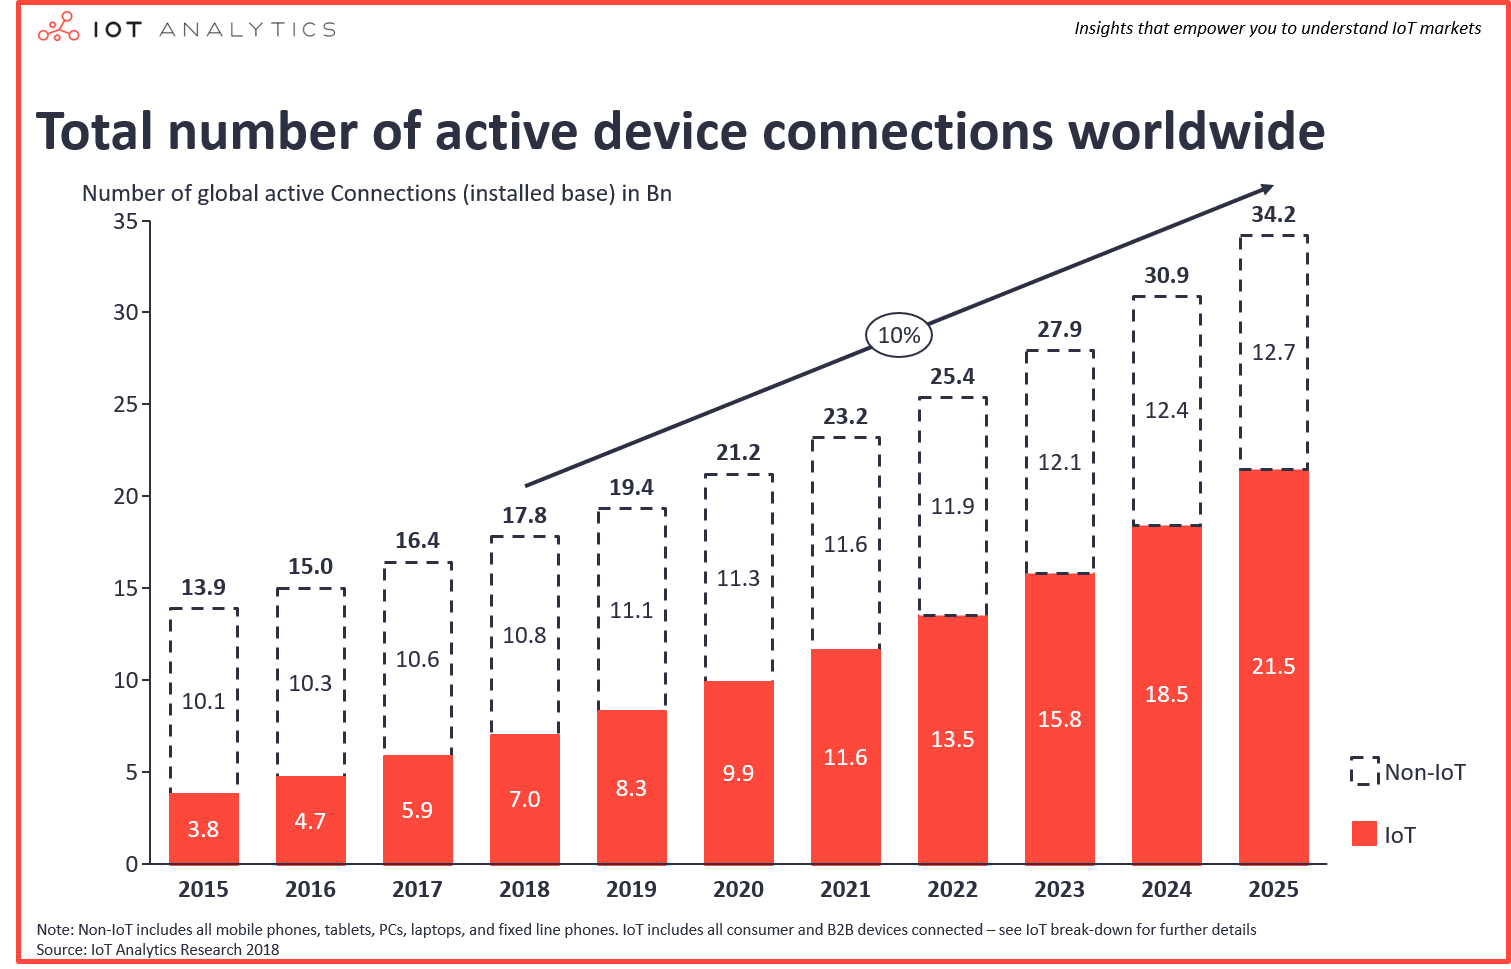
\includegraphics[width=\textwidth]{img/state_of_the_art/iot_number_connected.png}
  \caption{Nombre de dispositifs connectés à Internet \cite{lueth_2018}}
  \label{fig:iot_number}
\end{figure}

~

\noindent
Un réseau de communication unique et employable indépendamment du contexte du projet n'existe pas \cite{vannieuwenborg_iot}. Toutefois, une multitude de réseaux avec des caractéristiques distinctes sont disponibles, tels que LoRaWAN et GSM. La figure 1 présente l'architecture simplifiée des réseaux utilisés par les dispositifs IoT pour échanger des informations avec des serveurs ou des utilisateurs qui sont connectés à Internet. Nous ne nous intéressons ici qu'aux technologies responsables de la transmission de données dans la phase 1 de la figure.

~

\begin{figure}[ht!]
  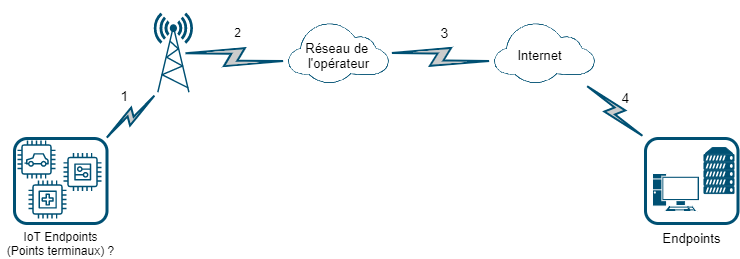
\includegraphics[width=\textwidth]{img/state_of_the_art/network_iot.png}
  \caption{Architecture simplifiée d'un réseau avec dispositifs IoT (Basé sur \cite{sanchez2016state, mekki2018overview})}
  \label{fig:network_archi}
\end{figure}

~

\noindent
Actuellement, les principaux réseaux sans fil disponibles pour les dispositifs IoT sont :

~

\begin{itemize}
  \item LoRaWAN
  \item Réseaux mobiles (2G/3G/4G/5G)
  \item Sigfox
  \item Satellite
  \item Wi-Fi
  \item Zigbee
  \item Bluetooth
  \item Réseaux mobiles IoT (NB-IoT et LTE-M)
\end{itemize}

~

\noindent
Ces technologies utilisent toutes des ondes électromagnétiques pour transmettre les données, mais les fréquences sur lesquelles elles opèrent sont parfois très différentes. Certaines technologies utilisent une implémentation propriétaire, d'autres se basent sur des standards open source. \cite{foubert_iot} De façon similaire, certaines technologies exploitent la bande ISM\footnote{Bande industrielle, scientifique et médicale}, alors que d'autres exploitent des fréquences non réglementées. Ces dernières permettent de déployer son propre réseau privé, à condition d'acheter et configurer tout le matériel requis ce qui peut demander un investissement initial assez important. Ces différences accordent des propriétés distinctes aux réseaux en ce qui concerne le coût d'utilisation et déploiement, la bande passante, et la portée du signal. À noter également, certains réseaux imposent une taille maximale sur chaque message, qu'il soit envoyé ou reçu. Le tableau comparatif de l'annexe \ref{ap:table_network} offre une vue d'ensemble sur les différentes technologies et leurs propriétés. Il faut cependant remarquer que la portée et le débit sont juste donnés à titre comparatif et ils sont à prendre avec des pincettes. En effet, ces valeurs varient beaucoup en fonction de certains paramètres tels que la géographie du milieu (urbain ou rural) et des éventuelles interférences. Néanmoins, le débit et la portée sont très importants pour classifier ces réseaux et, avec l'aide de la figure \ref{fig:range_iot}, ces technologies peuvent être classées de la façon suivante \cite{orange_iot} :


\begin{figure}
  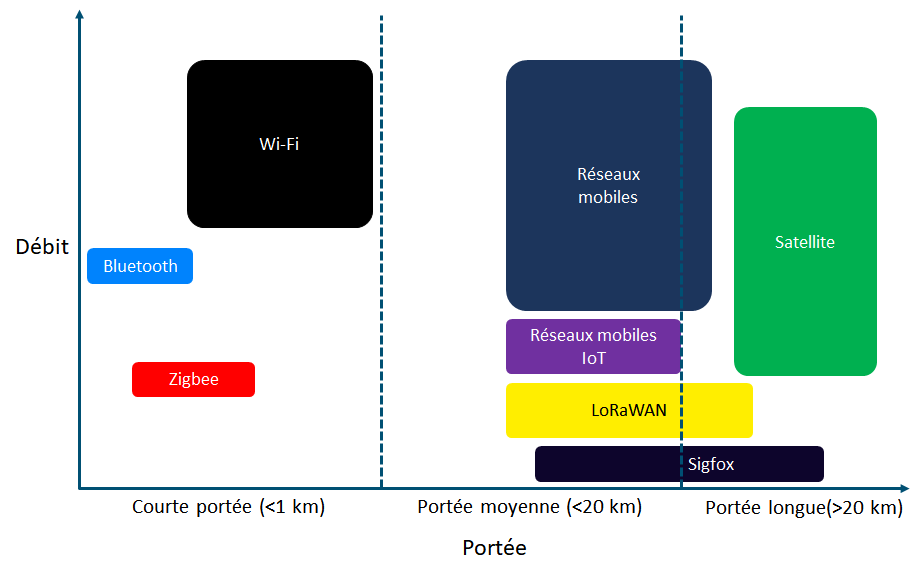
\includegraphics[width=\textwidth]{img/state_of_the_art/range_iot.png}
  \caption{Classement des réseaux en fonction de leur portée et débit (Basé sur \cite{mekki2018overview})}
  \label{fig:range_iot}
\end{figure}

~

\begin{itemize}
  \item \textbf{IoT haut débit :} Dans cette catégorie se trouvent principalement les technologies comme les réseaux mobiles, le Wi-Fi et le satellite. Les débits proposés sont généralement supérieurs au Mb/s. En contrepartie, l'utilisation de ces technologies engendre une consommation énergétique plus élevée.

  ~

  \item \textbf{IoT bas débit :} Ici se trouvent les réseaux mobiles IoT, LoRaWAN, Sigfox, et Zigbee. En fonction du réseau, le débit peut varier entre quelques bits par seconde jusqu'à un Mb/s. Ces technologies offrent une consommation énergétique faible.

  ~

  \item \textbf{IoT critique :} C'est-à-dire lorsqu'il s'avère nécessaire de transmettre des données sur un intervalle de temps donné \cite{orange_iot}. C'est une propriété des réseaux 5G.
\end{itemize}

~

\noindent
Un point également important est que ces technologies ont de différents niveaux de maturité. Au moins un réseau mobile est disponible dans chaque pays, mais les nouveaux réseaux comme Sigfox, LoRaWAN, et 5G sont en revanche toujours en cours de déploiement. De ce fait, ces dernières technologies ne sont disponibles que dans certaines régions possédant une infrastructure moderne. La couverture du réseau est un critère important à prendre en compte avant de faire un choix afin d'éviter les mauvaises surprises.
Finalement, toujours dues à ce différent degré de maturité, certaines technologies plus anciennes pourraient voir la fin de ses jours dans les années à venir. Par exemple, certains opérateurs vont décommissionner leur réseau 2G à partir de 2020 \cite{swisscom_2g}. Les opérateurs restants devraient suivre la même tendance dans les années suivantes. De plus, le réseau 3G devrait suivre la même tendance comme affichée sur la figure \ref{fig:evo_network}.

\begin{figure}[ht]
  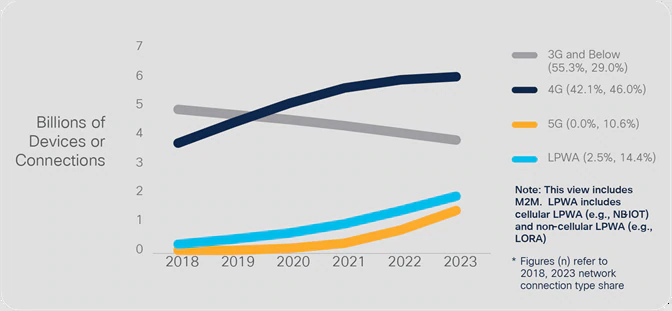
\includegraphics[width=\textwidth]{img/state_of_the_art/network_evolution.png}
  \caption{Évolution du nombre de dispositifs connectés aux différents réseaux \cite{report_cisco}}
  \label{fig:evo_network}
\end{figure}

~

\noindent
Comme il sera expliqué plus tard dans ce mémoire, le prototype doit être capable d’utiliser les réseaux de communication à distance. En effet, une connexion filaire à Internet n’est parfois pas disponible dans les structures de santé. Le choix de la technologie plus approprié sera présenté dans la section \ref{sec:sol_hard}.


\section{Monitoring de l'état d'un serveur linux}

\noindent
La nécessité de surveiller toute l'infrastructure IT, et en particulier des serveurs tournant sous Linux, existe depuis un bon nombre d'années. Cependant, surveiller un système n'est pas trivial. Cela peut être accompli de différentes manières en fonction des évènements ou statistiques qui doivent être observées dans la machine hôte. Par exemple, l'utilisation de logs pour débugger une application ou voir l'historique de transactions d'une base de données est une technique de monitoring utilisée depuis de nombreuses années. D'autres techniques de monitoring existantes sont le profiling, le tracing et l'acquisition de métriques \cite{brazil2018prometheus}. Dans cette section, seulement les technologies d'acquisition de métriques sont présentées puisqu'elles sont les plus utiles pour connaître l'état de la machine.

~

\noindent
Créé à la fin des années 80, le protocole SNMP \cite{RFC1098, RFC1157} permet de monitorer et configurer des dispositifs différents connectés au réseau. Tout au long des années, des solutions de monitorage de métriques de plus haut niveau, ou tout-en-un, sont apparues sur le marché. Ces solutions utilisent différents protocoles, dont SNMP, pour surveiller les dispositifs sur le réseau et stockent toutes les informations recueillies sur une base de données. De plus, elles permettent de définir un ensemble de conditions à surveiller de plus près et si une de ces conditions est violée, une alerte est transmise vers l'équipe responsable de l'infrastructure. Deux exemples de solutions créées à la fin des années 90 et qui demeurent disponibles sont Nagios et Zabbix.

~

\noindent
Actuellement, un grand nombre de solutions de monitoring sont disponibles sur le marché proposant différents modèles commerciaux. En effet, certaines solutions sont vendues comme un produit, mais d'autres préfèrent suivre un modèle open source. Dans le cas de ces dernières, les entreprises responsables de l'application proposent souvent leurs services en matière d'assistance technique afin d'installer et maintenir la solution. Un autre modèle aussi appliqué est de proposer une version gratuite avec un nombre limité de fonctionnalités, et une version payante débloquant toutes les capacités de l'application. Avant d'entamer toute recherche d'une solution, il faut comprendre quelle formule s'adapte le mieux aux besoins de l'utilisateur.
Comme il est affiché sur la figure \ref{fig:mon_archi}, deux architectures existent pour les solutions de monitoring : \textit{pull} et \textit{push} \cite{brazil2018prometheus, techhub_monitoring, blog_monitoring, techhub_monitoring}. Chaque application est entièrement basée sur une de ces deux approches. Dans certains cas, une solution peut parfois supporter les deux architectures (voir exemple figure \ref{fig:archi_prom_simple}). Cependant, ces solutions détiennent toujours un modèle préféré, et l'autre possibilité sert juste à combler certaines lacunes du premier modèle puisque, en effet, chaque architecture possède ses avantages et faiblesses.

~

\begin{figure}[ht!]
  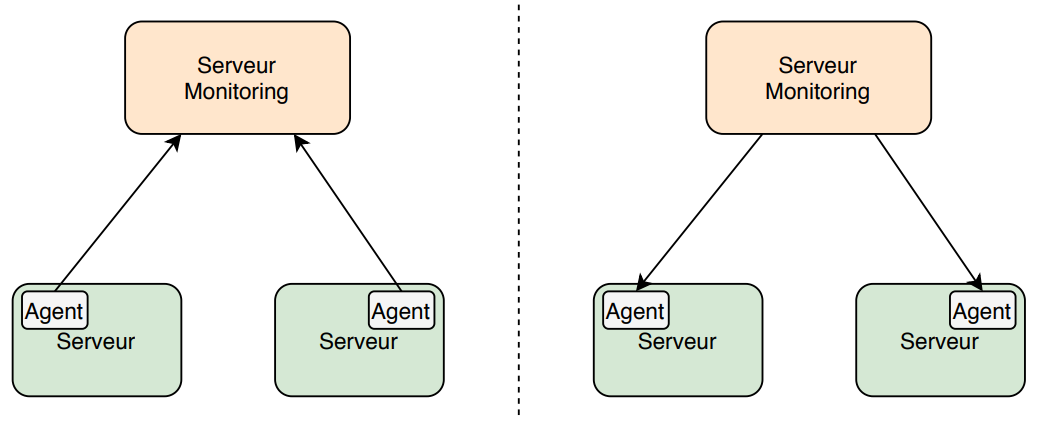
\includegraphics[width=\textwidth]{img/state_of_the_art/monitoring_architecture.png}
  \caption{\textbf{Gauche :} Solution de monitoring avec architecture \textit{push}.  \textbf{Droite :} Solution de monitoring avec architecture \textit{pull}.}
  \label{fig:mon_archi}
\end{figure}



\begin{figure}[ht!]
  \centering
  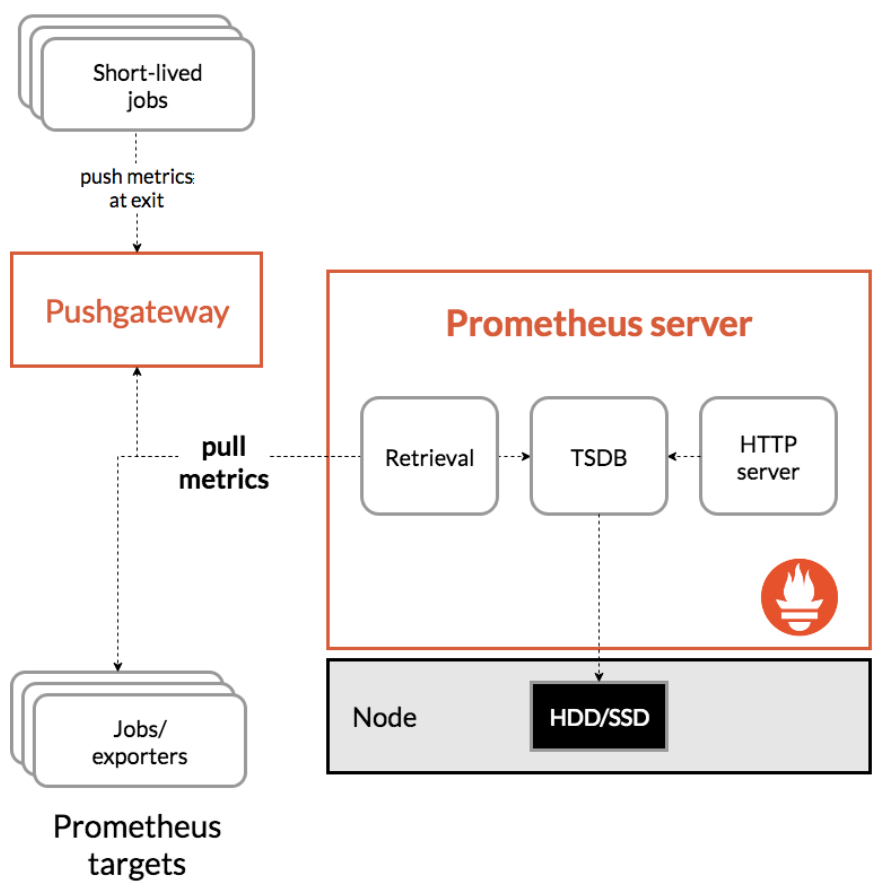
\includegraphics[scale=0.4]{img/state_of_the_art/prometheus_archi_simple.png}
  \caption{Architecture \textit{pull} de Prometheus. Le modèle \textit{push} est supporté grâce au Pushgateway.}
  \label{fig:archi_prom_simple}
\end{figure}

~

\noindent
Dans le modèle de type \textit{push}, les agents dans la machine hôte envoient un ensemble de métriques ou des événements au serveur de monitoring. Cette technique permet notamment de définir des conditions d'alerte dans l'agent, et c'est celui-ci qui se charge de vérifier ces conditions. Lorsque le test des conditions passe, l'agent transmet un événement au serveur de monitoring. De plus, seul le système de push est capable de correctement acquérir des données à propos de jobs Batch de courte durée. \cite{blog_monitoring, prometheus_tuto} En effet, comme affiché sur la figure \ref{fig:batch_end}, le modèle \textit{pull} peut rater la fin du job ce qui se traduit par une perte d'informations.

~

\begin{figure}[ht!]
  \centering
  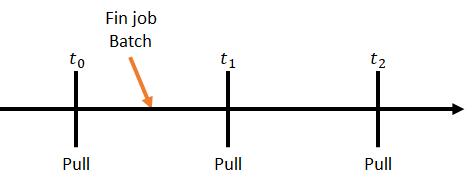
\includegraphics{img/state_of_the_art/pull_batch_miss.png}
  \caption{Faiblesse du modèle \textit{pull}. Le système de monitoring a raté les informations de la fin du job}
  \label{fig:batch_end}
\end{figure}

~

\noindent
Dans le modèle de type \textit{pull}, les agents dans la machine hôte collectent et exposent les métriques, mais c'est au serveur de monitoring d'activement aller retrouver ces données. Par conséquent, les événements et alertes au niveau des agents ne sont pas pris en charge, dans la mesure où ces derniers ne savent pas quand le système de monitoring récupérera les informations. En revanche, cette méthode permet de mieux identifier si un problème s'est produit sur la machine hôte puisqu'elle ne répondra plus aux requêtes lorsque cela a lieu.\cite{prometheus_doc_pull_push} Ceci rend l'approche \textit{pull} légèrement plus fiable que la technique \textit{push}. Les deux méthodes possèdent donc leurs avantages et inconvénients qu'il faut tenir en compte lors du choix de la technologie. Cependant, dans la majorité des cas, les deux architectures offrent ces capacités très similaires \cite{interview_push_pull}.

~

\noindent
Indépendamment de l'architecture utilisée, toutes les informations recueillies ou reçues par le serveur de monitoring doivent être stockées sur une base de données. Les solutions plus anciennes comme Nagios et Zabbix, utilisent principalement des bases de données relationnelles \cite{nagios_db, zabbix_db}. Ceci n'est plus le cas pour les solutions plus récentes telles que Prometheus et le TIG Stack\footnote{Le TIG stack est la combinaison de Telegraf, InfluxDB et Grafana pour créer un outil de monitoring} qui utilisent des bases de données orientées séries temporelles pour la persistance des données. Cette sorte de base de données, comme son nom indique, est mieux optimisée pour des valeurs horodatées \cite{time_series_fr}. En effet, ces bases de données possèdent les propriétés suivantes \cite{alibaba_timeseries}:

~

\begin{itemize}
  \item Elles supportent des écritures simultanées et avec de grands débits. Typiquement, dans ces bases de données se produisent énormément d'écritures, mais pas beaucoup d'accès.
  \item Ces bases de données doivent stocker d'énormes quantités de données temporelles. Elles utilisent des algorithmes de compression spécifiques pour stocker les données de manière efficace. \cite{di2007efficient}
  \item Toutes les requêtes sont effectuées sur base d'un intervalle de temps
  \item Les données ont une durée de rétention. À partir d'une certaine date, la base de données élimine automatiquement les informations car elles sont jugées non utiles.
\end{itemize}

~

\noindent
De ce fait, les bases de données orientées séries temporelles offrent un stockage plus efficace pour les métriques surveillées. Un dernier aspect très important d'une solution de monitoring est la visualisation de données. La majorité des solutions offrent soit un outil de visualisation propriétaire (Nagios ou Zabbix), soit elles exploitent des outils existants tels que Grafana (Prometheus et le TIG Stack).

~

\noindent
Le but principal de ce mémoire est de construire un système de monitoring pour CERHIS. Il est donc très important de comprendre ce qui se fait actuellement dans l'industrie et quels types de solutions sont disponibles à l'heure actuelle. Le logiciel de monitoring implémenté lors de ce mémoire sera décrit en détail dans la section \ref{sec:c_arch}.


\section{Plateformes de visualisation de données}

\noindent
La visualisation de données consiste à représenter plusieurs formats de données sous un format visuel tel que les graphiques. Le système visuel humain est capable d'identifier des tendances ou des aberrations. Le but de la visualisation des données consiste alors dans l'aide de la compréhension des données en exploitant cette capacité. \cite{zoo_data}

~

\noindent
Les outils de visualisations de données sont alors des solutions software qui aident à accomplir cet objectif. \cite{bikakis2018big} Ces outils fournissent une plateforme très puissante pour communiquer de l'information. Cependant, le concept de données est trop abstrait. En effet, elles peuvent être des coordonnées spatiales, les mesures de température d'une pièce, le nombre d'occurrences d'un évènement, le classement d'une course automobile, etc. Pour chacun de ces différents types de données, la méthode de visualisation à utiliser est différente. Par exemple, une carte serait utilisée pour afficher les coordonnées, mais une courbe serait préférée pour afficher l'évolution de la température. L'article \cite{zoo_data} propose différentes méthodes et graphiques pour observer les différents types de données existants.

~

\noindent
Comme présenté dans \cite{kirk2019data}, la visualisation de données doit respecter les trois principes suivants :

~

\begin{itemize}
  \item \textbf{Fiables (Dignes de confiances) :} Ce principe est fondamental, nous devons pouvoir faire confiance aux données qui nous sont présentées. Aucune manipulation doit être effectué sur la façon dont les données sont affichées afin de manipuler la perception de l’observateur. Par exemple, l’axe vertical d’un graphique à barres ne doit jamais être tronqué.

  ~

  \item \textbf{Accessibles :} La visualisation des données doit aider les observateurs à mieux comprendre et interpréter les données. Le contexte des observateurs est essentiel pour que la visualisation puisse être adaptée à leurs besoins. Cependant, cela doit être fait avec prudence et sans avoir un impact sur les données. Par exemple, un sujet complexe ne doit pas être simplifié à l'excès.

  ~

  \item \textbf{Élégante :} Une visualisation élégante des données doit captiver et retenir l’attention des observateurs. Toutefois, cela ne doit jamais compromettre les deux autres principes présentés ci-dessus.


\end{itemize}


~


\noindent
Avec l'arrivée de l'ère des Big Data, les technologies de visualisation sont devenues d'autant plus importantes. En effet, la quantité de données à traiter est devenue tellement importante qu'un humain n'est plus capable de le faire. Pour résoudre ce problème, de nouvelles technologies sont émergées, capables de mieux guider l'utilisateur à trouver des tendances dans les données. Actuellement, trois grandes catégories d'outils de visualisations de données sont disponibles :

~

\begin{itemize}
  \item Les librairies software, telles que Matplotlib ou D3.js, qui aident les utilisateurs à créer différentes visualisations de données. L'utilisation de ces librairies demande des compétences en programmation.

  \item Ensuite, il y a les outils purement dédiés à la visualisation de données tels que Grafana(fig. \ref{fig:graf_ex}) ou Google Data Studio. À partir d'une interface web, ces outils permettent de créer différentes visualisations en utilisant seulement des langages de requête comme SQL. Certains de ces outils sont capables d'aider l'utilisateur à formuler des requêtes. (Query Builders)

  \item Finalement, il y a les outils de Business Intelligence. Généralement, ils proposent les mêmes fonctionnalités qu'un outil de visualisation de données. Cependant, en plus de cela, ils permettent également de traiter les données et d'effectuer des prédictions grâce à celles-ci. Un exemple d'un tel outil est Tableau (fig. \ref{fig:tab_ex}) ou Power BI.
\end{itemize}

~

\noindent
Une bonne visualisation des données est essentielle pour avoir une solution de monitoring. En effet, une bonne visualisation permet de mieux évaluer l’état du système surveillé et d’identifier la source d’un problème plus rapidement. La section \ref{sec:c_arch} couvrira la manière dont une solution de visualisation de données a été intégrée au logiciel de monitoring.


\begin{figure}[ht!]
  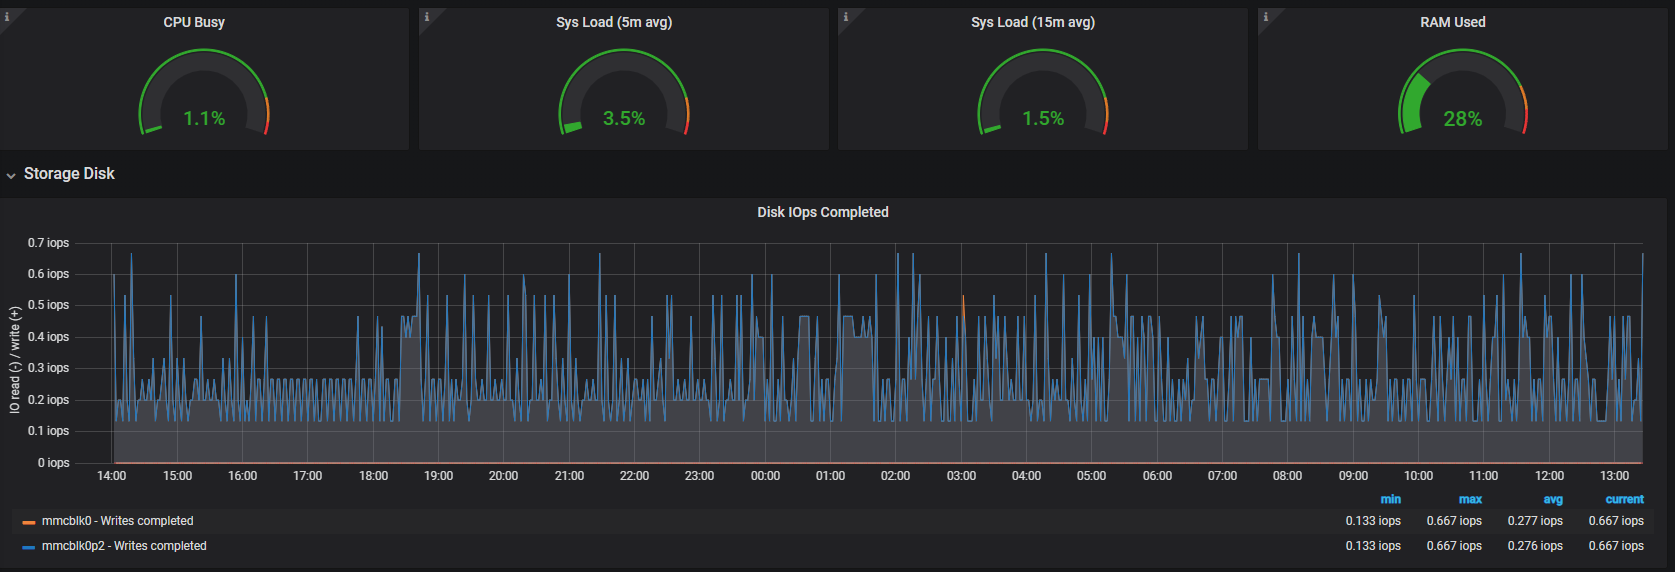
\includegraphics[width=\textwidth]{img/state_of_the_art/data_grafana.png}
  \caption{Exemple de visualisation de données avec Grafana}
  \label{fig:graf_ex}
\end{figure}


\begin{figure}[ht!]
  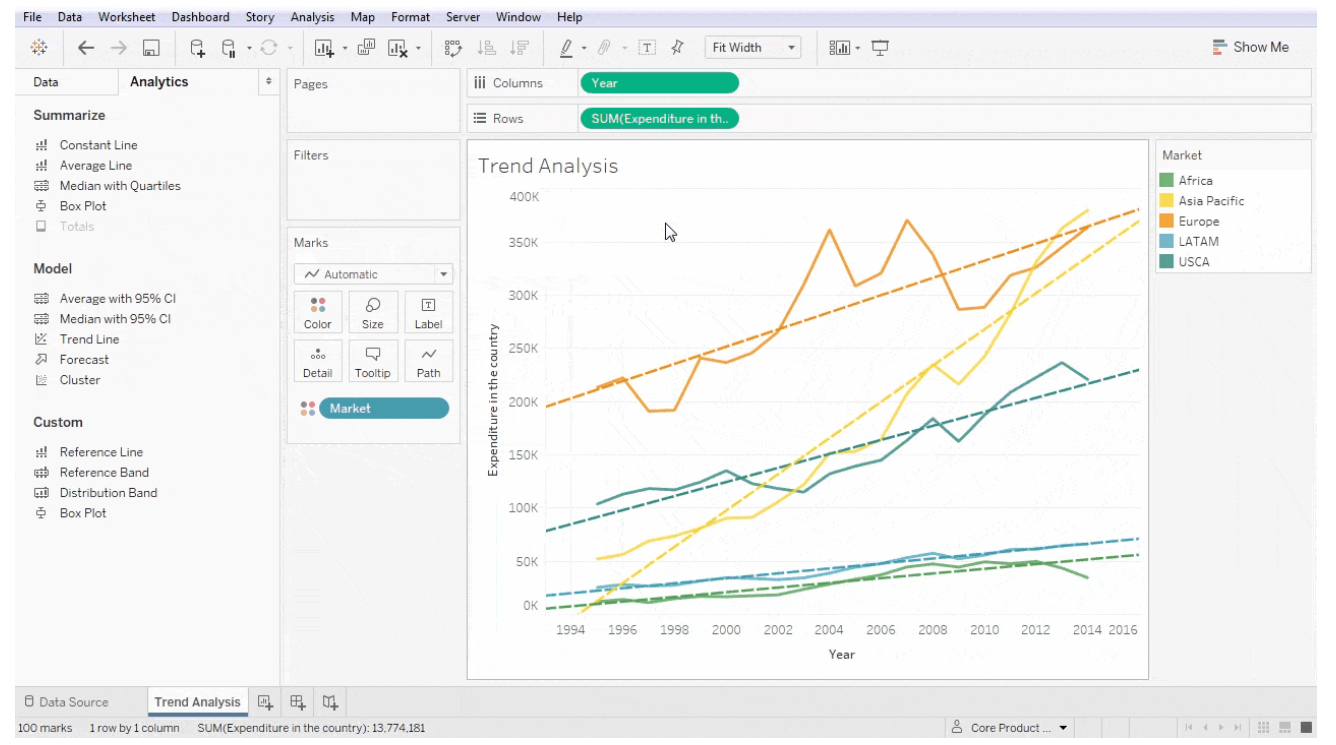
\includegraphics[width=\textwidth]{img/state_of_the_art/tableau.png}
  \caption{Exemple de visualisation et traitement de données avec Tableau \cite{tableau_ex}}
  \label{fig:tab_ex}
\end{figure}


\chapter{Cahier des charges}
\label{chap:3}

\noindent
Le but de ce mémoire consiste à développer un prototype capable de surveiller l'infrastructure de CERHIS et s'assurer du bon fonctionnement de celle-ci. De plus, ce système de monitoring doit pouvoir avertir un technicien lorsqu'un problème est détecté. Bien évidemment, pour accomplir cet objectif, le système devra acquérir des données sur le fonctionnement des différents dispositifs de CERHIS. Ces données devront être sauvegardées localement, mais aussi sur un serveur distant. Une interface web devra également être présente pour faciliter la visualisation de ces données, que cela soit dans le périmètre du centre hospitalier ou partout dans le monde. La figure \ref{fig:mon_archi_simple} reprend l'architecture simplifiée de ce système de monitoring.

~

\noindent
Pour simplifier la division du travail, la création du dispositif a été scindée en deux parties.
Une première partie majoritairement \textit{hardware} comportant le choix et l'assemblage de tous les composants nécessaires au développement du prototype. Cela englobe l'ordinateur requis pour tourner le logiciel, l'alimentation, la solution de communication et le logiciel qui permet aux différents composants de s'interfacer. Ensuite, une deuxième partie comprenant juste le logiciel nécessaire pour effectuer les tâches de monitoring. Cela comprend les fonctionnalités requises pour l'acquisition, traitement, stockage et visualisation des données. La présentation des spécificités de chaque partie se fera dans les sections suivantes (sections \ref{sec:cahier_proto} et \ref{sec:cahier_soft}).



\begin{figure}[ht!]
  \centering
  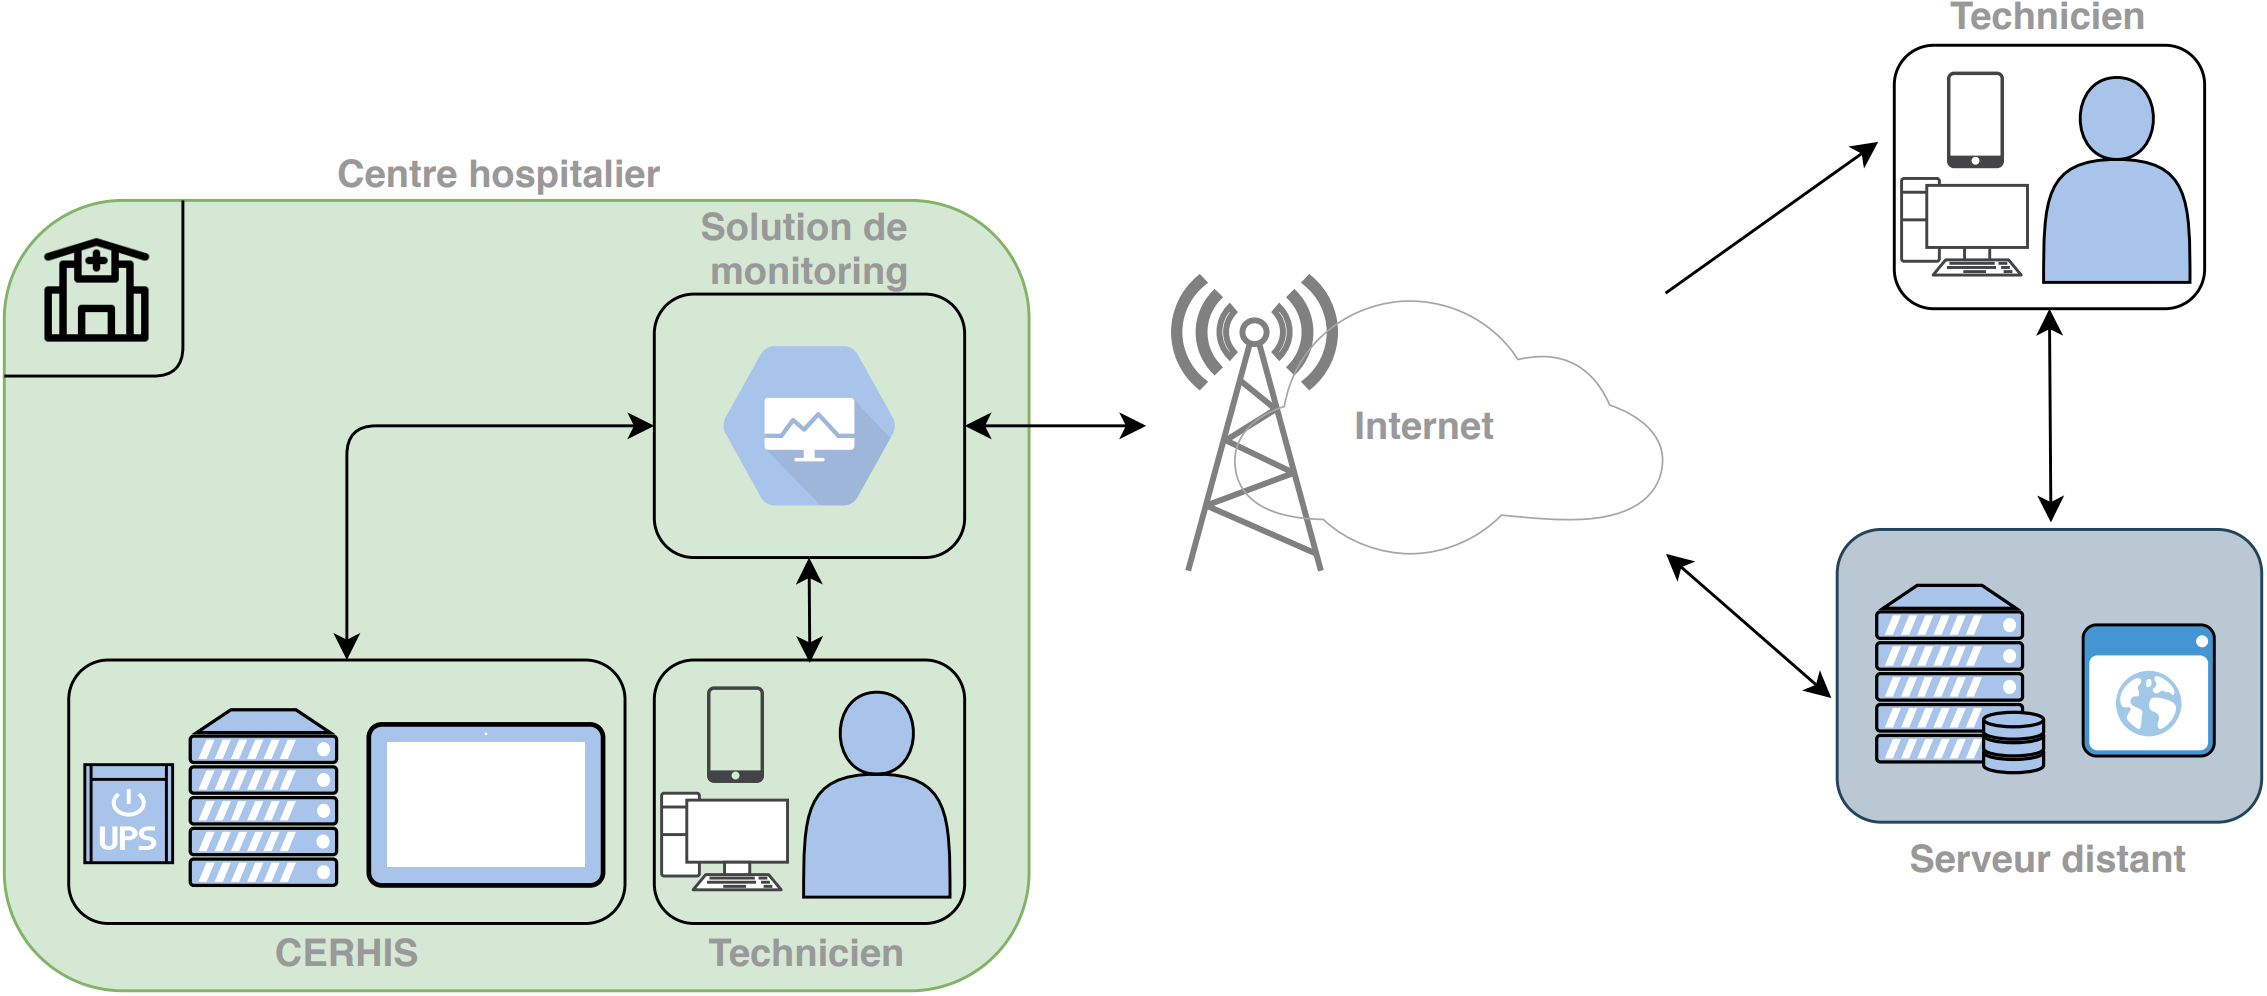
\includegraphics[width=\textwidth]{img/cahier_des_charges/baseline_archi.png}
  \caption{Architecture simplifiée de la solution de monitoring}
  \label{fig:mon_archi_simple}
\end{figure}

\section{Caractéristiques matérielles du dispositif}
\label{sec:cahier_proto}

Étant donné que le dispositif de monitoring sera utilisé dans des centres hospitaliers en Afrique centrale, il doit être capable de résister à certaines caractéristiques propres du milieu telles que la température. Voici la liste exhaustive de toutes les caractéristiques matérielles que le produit doit posséder :

~


\begin{itemize}
  \item Le prototype doit être robuste. Mes composants électroniques doivent notamment être capables de supporter des températures ambiantes supérieures à \SI{30}{\celsius} pendant de longues périodes. \cite{temperature_kinshasa}

  \item Le dispositif doit être capable de communiquer à distance, même lorsqu'une connexion à internet filaire n'est pas disponible. De ce fait, le prototype doit être capable de tirer parti d'une des technologies présentées dans la section 2 pour pouvoir envoyer des informations et des alertes.

  \item Le dispositif doit être d'apparence discrète, évitant d'attirer l'attention sur sa valeur.

  \item Le coût doit rester abordable et réaliste.

  \item Le dispositif doit posséder un système d'alimentation mixte capable d'alimenter le prototype pendant un ou deux jours en cas de passe du service électrique.

  \item Le boîtier doit être fermé hermétiquement pour empêcher des insectes d'y faire son nid.
\end{itemize}



\section{Fonctionnalités à implémenter}
\label{sec:cahier_soft}

Pour la section logiciel du dispositif, les fonctionnalités à implémenter peuvent encore être divisées en deux sous-sections : la solution de monitoring tournant sur le site, et le serveur distant capable de recevoir, stocker et afficher des données. Les fonctionnalités présentées ci-dessous seront alors divisées en suivant ces deux sous-sections.

~

\begin{itemize}
  \item \textbf{Solution de monitoring dans le centre hospitalier}
  \begin{itemize}
    \item Effectuer un mappage du réseau local de façon à trouver tous les appareils qui y sont connectés.

    \item Monitorer la présence des appareils connectés au réseau local. Si un appareil se déconnecte du réseau, pouvoir indiquer combien de temps est passé depuis sa dernière connexion.

    \item Monitorer l'état de fonctionnement du serveur de CERHIS.

    \item Envoi d'alertes par SMS.

    \item Envoi de données vers un serveur distant.

    \item Interface utilisateur permettant de facilement visualiser toutes les données.

    \item Vérifier le niveau de la batterie de CERHIS et l'état de charge des tablettes.

    \item Créer un historique de connexion des tablettes au serveur de CERHIS
  \end{itemize}

~

  \item \textbf{Serveur distant}
  \begin{itemize}
    \item Serveur capable de stocker les données envoyées depuis plusieurs centres hospitaliers.

    \item Interface utilisateur permettant de facilement visualiser toutes les données disponibles sur le serveur distant.
  \end{itemize}
\end{itemize}



\section{Priorité des tâches et méthodologie de travail}

\noindent
Les listes des fonctionnalités et caractéristiques présentes ci-dessus reprennent tout ce qui serait nécessaire pour avoir un produit fini. L'objectif de ce mémoire est bien évidemment d'essayer d'implémenter le maximum de fonctionnalités possibles. Cependant, le temps est limité et des imprévus peuvent survenir au long du chemin. De ce fait, les diverses fonctionnalités ont été classées par ordre de priorité afin de garantir que le prototype rendu à la fin de ce mémoire possède au moins un certain nombre de fonctionnalités.

~

\noindent
En premier lieu, c'était la sélection du matériel requis pour implémenter les fonctionnalités. Cela reprend, le choix de la plateforme, l'alimentation et la solution de communication. Cette tâche reprend aussi des tests sur la plateforme du projet de l'année précédente afin de vérifier si des changements étaient nécessaires.

~

\noindent
Deuxièmement, c'était l'implémentation de tout le code nécessaire pour lier les divers composants hardware. En particulier, l'implémentation du code essentiel pour mettre en marche la solution de communication. Ici s'ajoutent aussi les premiers essais afin de prouver le bon fonctionnement de la plateforme.

~

\noindent
Une fois la plateforme préliminaire choisie et testée, la possibilité de commencer à développer les différentes fonctionnalités du logiciel s'est ouverte. À nouveau, en raison du grand nombre de fonctionnalités requises, les plus cruciales ont été sélectionnées lors de réunions avec les parties prenantes. La liste ci-dessous présente les fonctionnalités triées par ordre décroissant de priorité :

~


\begin{itemize}
  \item Monitorer l'état du serveur, en particulier surveiller l'uptime de celui-ci et avertir un technicien en cas de modification anormale de la valeur.
  \item Mapper le réseau local.
  \item Surveiller la présence des dispositifs de CERHIS.
  \item Monitorer l'état de certains processus dans le serveur.
  \item Envoi des données vers un serveur distant.
  \item Interface web pour la visualisation des données
\end{itemize}

~

\noindent
Finalement, les dernières tâches reprennent la finalisation d'un boîtier permettant de loger les différents composants électroniques et des tests approfondis pour s'assurer du bon fonctionnement et la fiabilité de la solution de monitoring.

~

\noindent
Pour essayer d'être le plus efficace possible, la méthodologie de travail consistait à écrire toutes les tâches liées à ce projet sur des notes Post-it. Les Post-its orange représentaient les missions liées au software, et les jaunes correspondaient aux missions liées au hardware. Chaque note possédait aussi un numéro coïncidant avec la priorité de la tâche. Le critère de sélection était en premier lieu la couleur, orange prioritaire sur le jaune, et ensuite la priorité (lorsque les Post-its avaient tous la même couleur).


\chapter{Prototype}
\label{chap:4}

\section{Le premier prototype (2018-2019)}
\label{sec:old_boy}

\noindent
Dans le cadre du projet d'année de la première année du Master ingénieur civil en informatique, un prototype capable de surveiller l'infrastructure de CERHIS a été réalisé. Ce dispositif s'inspirait sur d'autres prototypes plus anciens créés par des étudiants de l'École polytechnique de Bruxelles. L'architecture du dispositif produit l'année dernière est présentée sur la figure \ref{fig:archi_prev}.

~

\begin{figure}[ht!]
  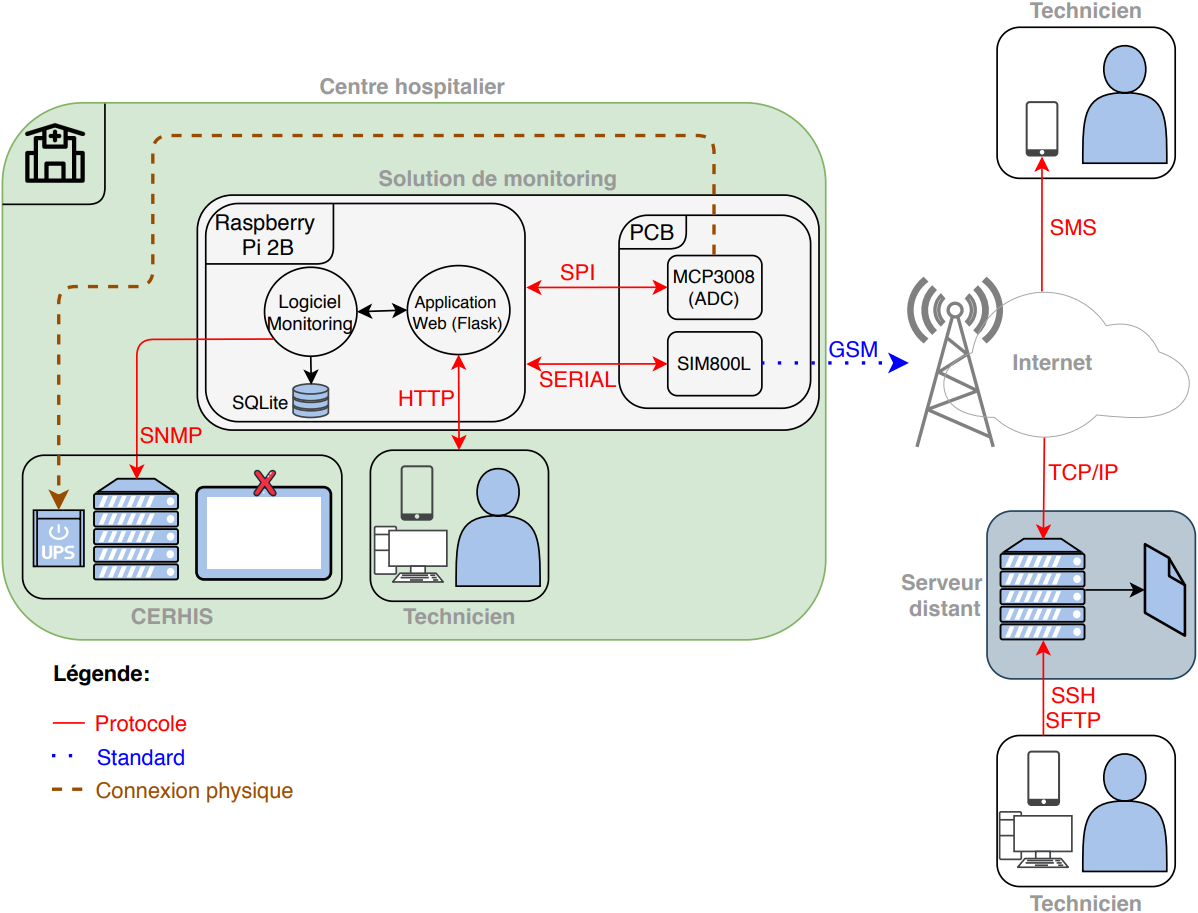
\includegraphics[width=\textwidth]{img/el_prototype/archi_prev.png}
  \caption{Architecture de la solution de monitoring développée lors de l'année académique 2018-2019}
  \label{fig:archi_prev}
\end{figure}



\noindent
Un Raspberry Pi 2B était utilisé pour tourner le logiciel de monitoring ainsi que l'interface web permettant la configuration de celui-ci. Un circuit imprimé (PCB) avait été réalisé dans le but de loger des composants électroniques différents tels que le module de communication GSM SIM800L et le convertisseur analogique numérique MCP3008. Ce même circuit imprimé s'insérait sur les ports GPIO du Raspberry Pi afin que ce dernier puisse interfacer avec les différents composants présents sur le PCB. Grâce au SIM800L, le réseau GSM d'un opérateur mobile local pouvait être utilisé pour envoyer des SMS vers un technicien, ou des informations quelques conques vers un serveur distant. Le MCP3008 était connecté à la batterie de CERHIS dans le but de monitorer la tension électrique de celle-ci. Dans ce premier essai, le serveur distant était juste capable de recevoir les données envoyées par le prototype et de les stocker sur un fichier \textit{.txt}. Aucun traitement ou visualisation des données n'était offert aux techniciens. De plus, le monitoring des tablettes n'a pas pu être implémenté par manque de temps.

~

\noindent
De façon à alimenter le dispositif, un système d'alimentation mixte avait été mis en place. Comme le montre la figure \ref{fig:power_source}, ce système était basé sur une batterie acide-plomb de 12V, un régulateur de charge permettant de recharger la batterie et un convertisseur step-down transformant la tension de 12 à 5 volts.

~

\begin{figure}[ht!]
  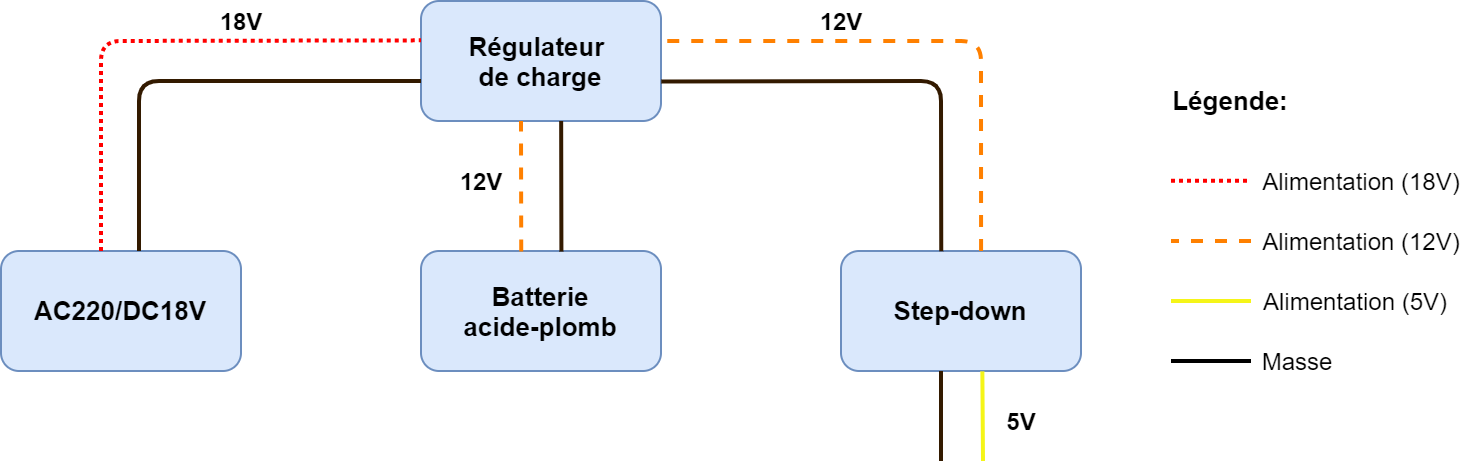
\includegraphics[width=\textwidth]{img/el_prototype/power_source.png}
  \caption{Système d'alimentation de la solution de monitoring développée lors de l'année académique 2018-2019}
  \label{fig:power_source}
\end{figure}

~

\noindent
Ce prototype a été testé pendant plusieurs semaines\footnote{entre le 14 mars et le 10 avril 2019} à Goma par un étudiant de l'ISIG\footnote{Institut supérieur d'informatique et de gestion de Goma}. Lors de cette période de tests, plusieurs problèmes ont été identifiés. Ils seront présentés dans la section suivante.

\subsection{Problèmes détectés}

\noindent
Plusieurs protocoles de tests avaient été mis en place l'année dernière dans le but d'évaluer ce premier dispositif. Les soucis qui ont été trouvés lors de ces tests peuvent être classés selon trois grandes catégories : communication, alimentation et température. Tous les problèmes sont documentés ci-dessous.

~

\begin{itemize}
  \item \textbf{Communication :}
  \begin{itemize}
    \item Corruption de certaines données échangées entre le SIM800L et le Raspberry Pi. Des bits semblaient être modifiés lors de la transmission des messages entre les deux composants. Cela provoquait une perte d'informations. De plus, cela rendait plus difficile l'utilisation du SIM800L, car ce dernier n'était pas capable de traiter toutes les commandes qui lui étaient envoyées.

    \item Implémenter toutes les fonctionnalités de communication requises avec le SIM800L était très laborieux. En effet, ce module peut être vu comme un automate fini déterministe. Des commandes AT sont utilisées pour contrôler le module, c'est-à-dire qu'elles sont employées pour changer l'état de celui-ci. Une succession correcte de multiples commandes est nécessaire afin d'accomplir une simple tâche telle que l'envoi d'un SMS. Ceci rendait le procès d'implémentation assez long, en particulier l'implémentation de la gestion des erreurs. Le problème mentionné ci-dessus a encore plus aggravé la complexité de la manipulation de ce module.
  \end{itemize}

~

  \item \textbf{Alimentation :}
  \begin{itemize}
    \item Le régulateur de charge initialement utilisé est tombé en panne lors de la réalisation des tests. Un simple remplacement de cette pièce semble avoir résolu le problème.

    \item Le step-down est tombé en panne lors des tests. Malheureusement, aucun remplacement pour cette pièce a été trouvé à Goma. Ce souci est possiblement lié au problème de température qui sera présenté ci-dessous. Cependant, n'ayant pas assez d'information pour prouver l'existence d'un lien de causalité, chaque problème doit être considéré séparément.
  \end{itemize}

~

  \item \textbf{Température :}
  \begin{itemize}
    \item D'après les personnes en charge de tester le prototype, celui-ci semblait atteindre de hautes températures. Des températures élevées peuvent avoir un impact considérable sur la durée de vie des différents composants électroniques.
  \end{itemize}
\end{itemize}

% \subsubsection{Influence sur le nouveau prototype}

\section{Nouveau Prototype}

\noindent
Compte tenu des problèmes rencontrés l'année précédente, un nouveau prototype a dû être conçu. Toutefois, énormément d'informations ont été acquises au cours de l'année dernière. Il ne serait pas judicieux de partir de zéro, car cela demanderait un effort assez important pour atteindre le niveau précédent. Ce nouveau prototype correspond alors à une évolution du résultat de l'année antérieure, ayant comme but de combler toutes les lacunes de ce dernier. Le choix de remplacer chaque composant est abordé ci-dessous.

\subsection{Solutions considérées}
\label{sec:sol_hard}

\subsubsection{Choix de la plateforme}

\noindent
Lors de l'année précédente, un Raspberry Pi 2B a été utilisé en tant que plateforme principale du projet. Ce modèle en particulier avait été choisi en raison de sa consommation énergétique plus faible que celle des modèles suivants, tout en offrant des performances amplement suffisantes. Depuis le projet antérieur, une nouvelle version est disponible sur le marché, le Raspberry Pi 4. Cependant, ce dernier présente une consommation énergétique encore plus élevée sans offrir de nouveaux avantages au projet. De ce fait, puisque le Raspberry Pi 2B s'est montré très fiable et qu'il restera en production jusqu'en 2026 \cite{rasp_prod}, il sera à nouveau utilisé dans ce nouveau prototype. Dans l'annexe (ajouter\_annexe), le tableau comparatif de toutes les solutions considérées l'année dernière est présent à titre de référence.


\subsubsection{Solution de communication}

\noindent
La communication à distance est probablement un des éléments les plus complexes de ce projet. En effet, l'infrastructure des différents réseaux en Afrique Centrale est sous-développée comparée à l'infrastructure en Europe. De plus, la partie de la communication est celle qui a apporté le plus de problèmes l'année précédente, et celle dont les problèmes sont les plus difficiles à résoudre. De ce fait, cette partie doit être abordée avec caution et la décision doit être très pondérée.

~

\noindent
Actuellement, le choix de réseaux accessibles en Afrique centrale est très restreint. En particulier, les réseaux orientés IoT (LTE-M, NB-IoT, Sigfox, LoRaWAN) ne sont actuellement pas disponibles dans la majorité des pays en Afrique Centrale ou leur couverture est extrêmement limitée.
De plus, les réseaux Sigfox et LoRaWAN\footnote{Les contraintes sur la quantité de données pour les réseaux LoRaWAN ne sont applicables que sur les réseaux publics.} sont très contraignants sur la quantité de données qui peut être envoyée sur une journée. De ce fait, ils ne s'encadrent pas dans le cahier des charges de ce projet. Le satellite aurait été le choix incontestable si le coût n'était pas un facteur limitant. Les options restantes telles que le Wi-Fi et le Bluetooth ont une portée très courte.  Les réseaux mobiles se présentent donc comme étant le meilleur compromis entre disponibilité, coût et consommation énergétique. L'accès à ces derniers est relativement facile, et la couverture des réseaux 2G et 3G semble être relativement bonne dans les régions plus densement peuplées. \cite{coverage_airtel, coverage_orange}


~

\noindent
Toutefois, le développement des réseaux mobiles orientés IoT (NB-IoT et LTE-M) dans ces pays doit être suivi de près au cours des prochaines années. Ils s'encadrent dans l'esprit de ce projet et offrent potentiellement un meilleur compromis que les réseaux mobiles classiques en raison de leur faible consommation énergétique.  Un autre aspect important à surveiller est la suppression des réseaux 2G au cours des années qui suivent. Cependant, vu le retard de l'infrastructure dans certains pays d'Afrique Centrale, il est très peu probable que cela ait lieu prochainement.

~

\noindent
Les réseaux mobiles proposent plusieurs protocoles pour transmettre des données. Afin de choisir le protocole le plus approprié pour ce projet, il est d'abord nécessaire de comprendre exactement quels types de communication sont requis. En premier lieu, il faut considérer la communication de machine à personne. Le prototype doit être capable d'envoyer un message d'alerte à un technicien. Le cahier des charges impose que ce type de communication soit effectué par SMS. Les techniciens ayant tous accès à un téléphone, cette méthode semble être la plus efficace pour communiquer avec eux.

~

\noindent
Ensuite, il y a la communication de machine à machine (M2M). Le prototype doit être capable d'envoyer les données recueillies vers un serveur distant qui les rendra accessibles aux techniciens. Cet échange de données peut être effectué également par SMS. Cependant, comme démontré dans le rapport de l'année dernière, le SMS est une méthode très coûteuse pour l'envoi de données M2M. D'autres protocoles permettent de transporter des données à un moindre coût comme l'USSD et le GPRS/HSPA/LTE. De ce fait, une comparaison a été effectuée afin de comprendre les avantages de chaque protocole, ainsi que celui qui est le plus approprié pour ce prototype.


~

\noindent
L'USSD, ou Unstructured Supplementary Service Data, est un protocole de communication présent dans les réseaux mobiles (GSM, 3G, 4G) qui permet à un client de communiquer avec les serveurs de l'opérateur du réseau mobile. L'USSD est un stateful protocol et les échanges de données entre le client et le serveur se font en temps réel.  Les opérateurs utilisent très souvent ce protocole pour donner accès à certains services spéciaux, tels que vérifier le solde restant dans une carte prépayée ($\*XXX\#$). L'USSD présente la caractéristique intéressante que toutes les connexions initiées par le client sont toujours routées vers les serveurs de l'opérateur de la carte SIM, même lorsque le client se trouve en itinérance \cite{lakshmi2017ussd}. Cela garantit que, indépendamment du lieu où se trouve le client dans le monde, l'échange d'informations se déroule toujours de manière similaire. De plus, cela permet aussi de diminuer les coûts élevés souvent associés à l'itinérance. Mais le protocole USSD possède bien d'autres avantages tels que :

~

\begin{itemize}
  \item Aucune configuration supplémentaire n'est requise pour utiliser l'USSD dans le réseau d'un opérateur. Au contraire, l'Access Point Name doit être configuré avant d'avoir accès au service GPRS.

  \item Le protocole USSD utilise moins de ressources d'un modem ou du réseau d'un opérateur que le GPRS. \cite{global_ussd}

  \item Le protocole USSD reste disponible même lorsque la connectivité à Internet du réseau est coupée. En contrepartie, cela rendrait le service GPRS inexploitable.\cite{transport_ussd}

  \item La majorité des modems sur le marché, dont le SIM800L, sont compatibles avec USSD. \cite{lakshmi2017ussd}
\end{itemize}

~

\noindent
Cependant, le protocole USSD possède aussi les désavantages suivants :

~

\begin{itemize}
  \item Déployer une application utilisant USSD est très difficile puisque cela demande de travailler de très près avec un opérateur de télécommunications. En effet, toutes les connexions sont dirigées vers les serveurs de ces derniers. \cite{perrier2015ussd}

  \item Lié au problème précédent, le protocole USSD ne donne pas directement accès à Internet. De ce fait, il n'est par exemple pas trivial d'utiliser un protocole application tel que HTTP pour envoyer des données vers un serveur.
\end{itemize}

~

\noindent
Pour pallier ce dernier problème, une solution assez particulière est exploitée actuellement dans certains pays en Afrique \cite{africa_ussd}. Elle permet aux utilisateurs d'accéder à des services qui ne sont disponibles que sur Internet, mais à travers le protocole USSD. La figure \ref{fig:ussdex} illustre comment fonctionne cette solution. Le serveur USSD joue le rôle de proxy et convertit les messages USSD initialement envoyés par le client en requêtes HTTP à envoyer à un serveur distant. Malheureusement, cette solution n'est disponible que dans un nombre restreint de pays, mais une solution similaire pourrait être éventuellement utilisée pour envoyer les données au serveur distant.

\begin{figure}[ht!]
  \centering
  \includegraphics[width=0.90\textwidth]{img/el_prototype/ussd_examples.png}
  \caption{Architecture simplifiée d'une solution USSD permettant d'accéder à des services sur Internet}
  \label{fig:ussdex}
\end{figure}

~

\noindent
L'alternative à l'USSD est de recourir aux normes General Packet Radio Service (GPRS), High Speed Packet Access (HSPA) ou Long Term Evolution (LTE) pour transmettre des données. Ces normes permettent de communiquer des données à travers le réseau de l'opérateur et fournissent au client un accès à Internet. Les protocoles de la couche application tels que HTTP sont très souvent utilisés en conjonction avec ces normes. Un exemple est l'emploi d'un smartphone connecté à Internet par le biais de données mobiles pour accéder à un site web. Ce niveau d'abstraction supplémentaire facilite l'utilisation de cette solution.

~

\noindent
Trancher entre l'USSD et le GPRS n'est pas simple. D'une part, l'USSD semble offrir une solution très fiable qui est couramment employée dans plusieurs pays africains. De l'autre côté, le GPRS permettrait d'exploiter les avantages d'une connexion standard à Internet et tous les protocoles d'application qui viennent avec. De ce fait, une comparaison entre les possibles de chaque solution a été effectuée.


~


\textbf{Solution 1: Routeur LTE (GPRS/HSPA/LTE)}

\vspace{-0.2cm}
~

\noindent
Dans cette première implémentation, l'idée était de remplacer le module SIM800L par un routeur LTE. Ce type de routeur est capable de se connecter aux réseaux mobiles afin de permettre aux clients d'accéder à Internet. Toute la partie bas niveau des réseaux serait alors traitée par le Raspberry Pi et le routeur. De ce fait, le logiciel de monitoring n'aurait besoin que d'utiliser des protocoles de la couche application, simplifiant donc l'implémentation du logiciel. Certains de ces routeurs peuvent aussi être raccordés à un deuxième réseau WAN\footnote{Wide Area Network ou réseau étendu en français}, comme une potentielle connexion Internet du centre hospitalier. Cette solution est la seule à proposer ce type de redondance. Cependant, les routeurs 4G sont assez coûteux, principalement ceux destinés à des environnements industriels. Un investissement d'au moins 70 ou 80 euros serait requis pour acquérir tel dispositif. De plus, leur consommation énergétique est assez élevée comparée au SIM800L puisque les routeurs proposent un grand nombre de fonctionnalités telles que le Wi-Fi et plusieurs ports Ethernet. La figure \ref{fig:so1} illustre l'architecture simplifiée de cette solution.

\begin{figure}[ht!]
  \centering
  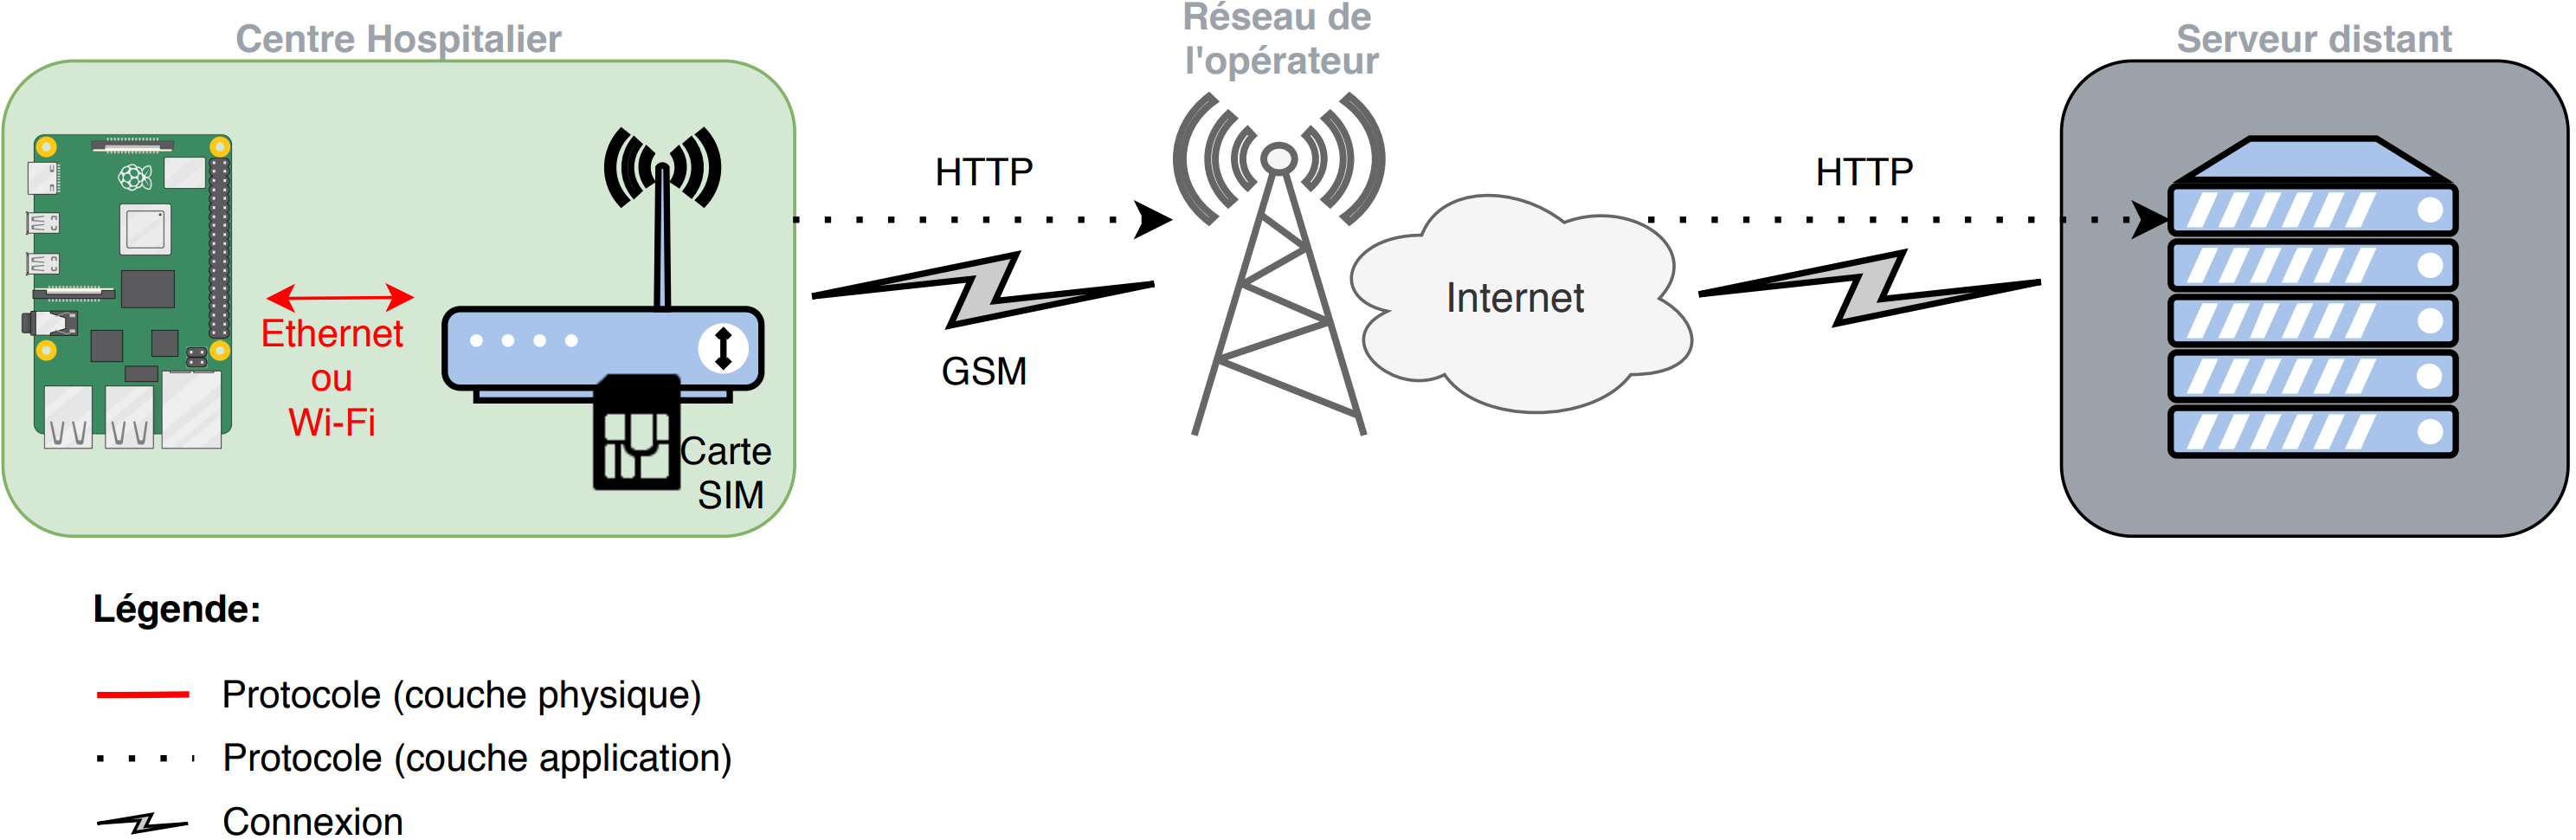
\includegraphics[width=0.93\textwidth]{img/el_prototype/solution1_com.png}
  \caption{Architecture simplifiée de la solution de communication avec un router LTE}
  \label{fig:so1}
\end{figure}

~

\newpage

\textbf{Solution 2: Service USSD avec SIM800L}

\vspace{-0.2cm}
~

\noindent
Jusqu'à il y a quelques années, déployer une application USSD était assez complexe puisque l'aide d'un opérateur était nécessaire \cite{perrier2015ussd}. Toutefois, sont apparues récemment sur le marché des entreprises qui offrent des services de communication exploitant la technologie USSD. En fonction de l'entreprise en question, la couverture du service ainsi que ses fonctionnalités diffèrent. Utiliser une telle solution permet de très aisément exploiter les avantages du protocole USSD tout en mitigeant ses défauts. Thingstream est un service de communication qui exploite la technologie USSD pour permettre des dispositifs de communiquer entre eux presque partout dans le monde. Cette plateforme se distingue par le fait qu'elle propose le protocole MQTT sur le protocole USSD. De ce fait, comme pour la solution précédente, le logiciel de monitoring a accès à un protocole de la couche application ce qui facilite l'échange de données, mais son choix est imposé. La solution de Thinsgtream sera présentée plus en détail dans la section \ref{sec:thingstream}.

~

\textbf{Solution 3: SIM800L et protocole point à point}

\vspace{-0.2cm}
~

\noindent
Dans cette implémentation, le SIM800L est à nouveau exploité. En effet, l'architecture est très similaire à celle du prototype de l'année dernière, la différence réside dans l'emploi d'un protocole de plus haut niveau pour communiquer avec le modem. L'année précédente, les commandes AT étaient envoyées par le logiciel de monitoring au SIM800L à travers le protocole SERIAL. Pour simplifier ce processus, il est possible d'utiliser le protocole point à point (PPP). Ce protocole de la couche liaison de données gère toute la complexité des commandes AT et permet au Raspberry Pi de se connecter à Internet. Le logiciel de monitoring peut donc de recourir aux protocoles habituels de la couche application pour échanger les données avec le serveur distant. Veuillez noter que le protocole SERIAL est toujours utilisé dans la couche physique. La figure \ref{fig:so2} illustre le fonctionnement de cette solution.


\begin{figure}[ht!]
  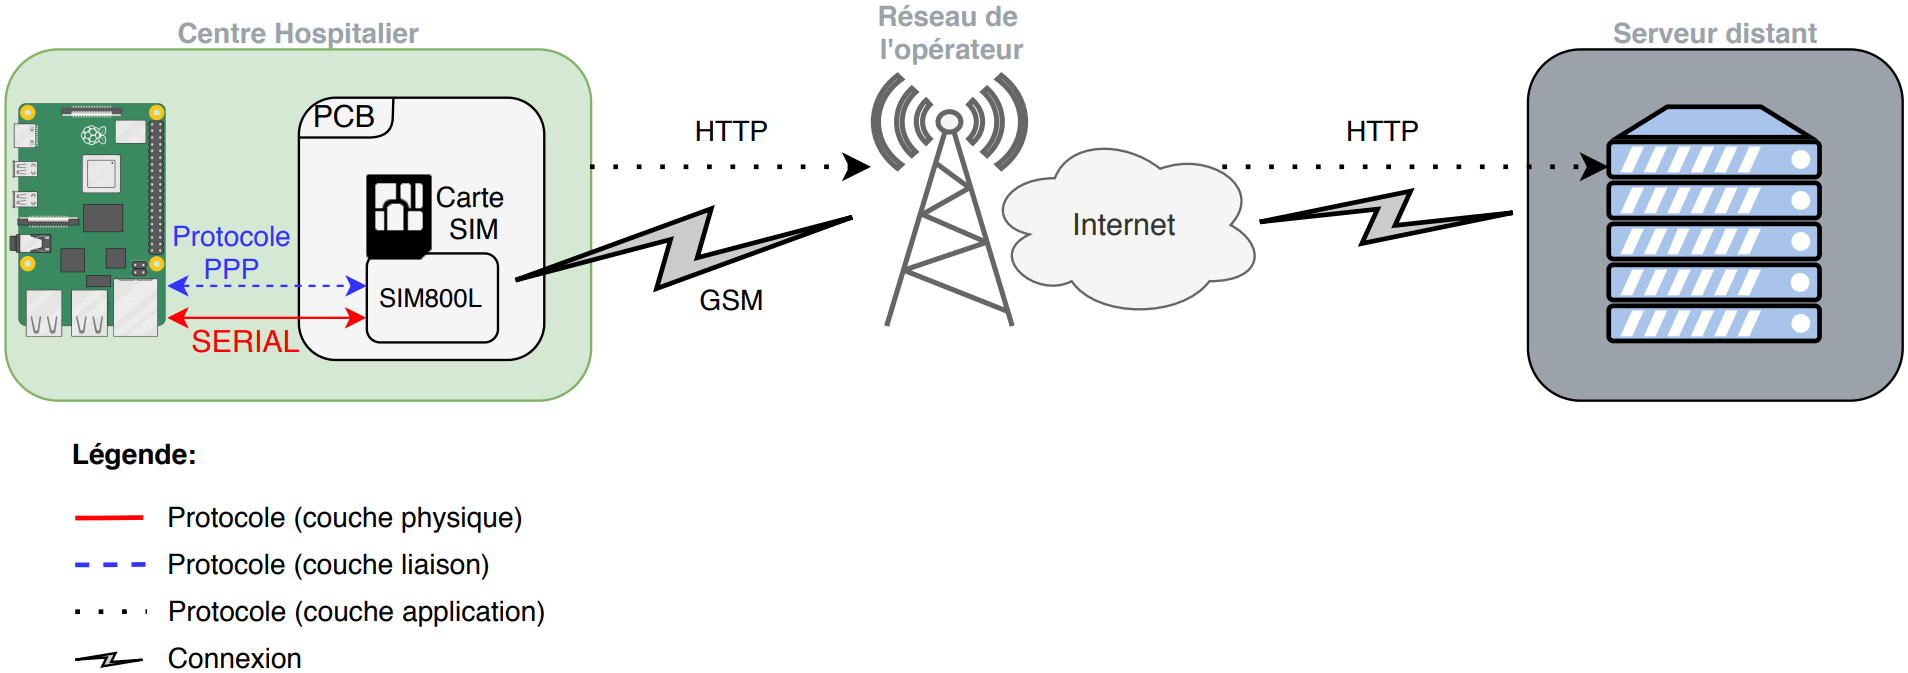
\includegraphics[width=\textwidth]{img/el_prototype/solution3_com.png}
  \caption{Architecture simplifiée de la solution de communication avec le SIM800L et le protocole PPP}
  \label{fig:so2}
\end{figure}

\noindent
Finalement, la solution 2 (USSD) est celle qui a été implémentée lors de ce mémoire. La solution 1 demandait un investissement assez élevé. De plus, il n'y a pas énormément d'informations sur la qualité des réseaux en République Démocratique du Congo \cite{congo_tower}. De ce fait, utiliser une solution basée sur le protocole USSD est le choix le plus sûr puisque, théoriquement, ce protocole fonctionne même lorsque la connectivité Internet du réseau est indisponible.

~

\noindent
Veuillez noter que la troisième solution ne possède pas le même problème de coût que la première. Cependant, cette solution a seulement été identifiée quelques semaines plus tard que les deux autres et, à ce stade, la deuxième méthode avait déjà commencé à être implémentée. En outre, la troisième proposition reste théoriquement moins fiable qu'une solution basée sur USSD. De ce fait, il a été décidé de continuer l'implémentation de la deuxième méthode afin d'augmenter la probabilité d'avoir une solution complètement fonctionnelle à la fin de ce mémoire. Utiliser le temps disponible pour implémenter les deux solutions parallèlement pourrait conduire à des solutions sous-optimales ou non fonctionnelles.

\subsubsection{Alimentation}

\noindent
Le système d'alimentation créé l'année dernière a aussi présenté des problèmes. En effet, le régulateur de charge ainsi que le step-down sont tombés en panne. Cependant, l'idée semblait prometteuse et, en particulier, l'autonomie du système était très bonne. Par conséquent, le plan pour ce mémoire fut de poursuivre avec la même idée, mais de changer deux choses. Premièrement, le step-down précédent a été remplacé par un nouveau modèle mieux documenté. Ce nouveau step-down est le XL4015.

~

\noindent
Le XL4015 est un convertisseur Buck capable de supporter une tension d'entrée comprise entre 8V et 36V et des charges allant jusqu'à 5A. Le rendement de ce convertisseur est très élevé pouvant atteindre les $96\%$. Des applications typiques pour ce step-down sont des moniteurs LCD et des appareils télécom ou réseaux. Cette dernière application s'encadre dans ce projet puisqu'un modem est inclus dans le prototype.


\begin{figure}[ht!]
  \centering
  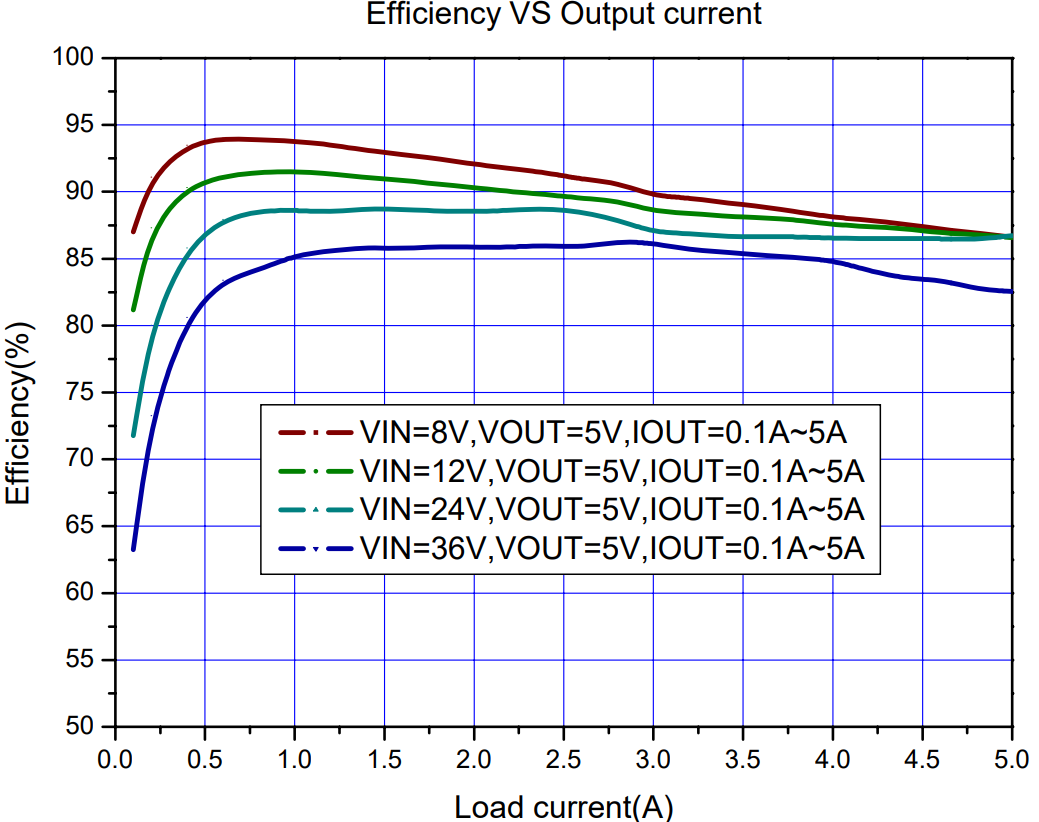
\includegraphics[scale=0.4]{img/el_prototype/rendement.png}
  \caption{Courbe de rendement du XL4015 lorsque $V_{out} = 5V$ \cite{xl4015_datasheet}}
  \label{fig:xlrend}
\end{figure}
~

\noindent
Ensuite, l'approche pour tester le système d'alimentation a été modifiée. Dans un premier temps, le prototype a été seulement alimenté à partir d'un chargeur de 12V. La batterie et le régulateur de charge n'étaient alors pas utilisés. Si le temps le permettait, le prototype serait testé avec la solution d'alimentation complète lors d'une deuxième phase. Ces tests déphasés ont comme but de mieux aider à identifier le composant provoquant les problèmes


\subsubsection{Boîtier}

\noindent
Une fois les composants définis, il ne restait plus qu'à choisir le boîtier. L'importance de celui-ci ne doit pas être sous-estimée. En effet, le problème de température du prototype précédent était probablement lié à la mauvaise ventilation de la boîte. De plus, le boîtier utilisé précédemment n'était pas adapté pour loger les composants électroniques différents. Les modifications requises pour l'ajuster aux composants n'étaient pas simples à effectuer et l'accès aux divers ports I/O du Raspberry Pi était très limité. Cependant, avant de partir sur la conception de la nouvelle boîte, plusieurs tests ont été réalisés sur l'ancien boîtier afin d'examiner les problèmes de température et la nécessité d'ajouter un ventilateur. Les résultats de ces tests seront présentés dans la section \ref{sec:prototests} et le nouveau design sera abordé dans la section \ref{sec:protores}.

\subsection{Thingstream}
\label{sec:thingstream}

\noindent
Thingstream est une entreprise qui propose \textit{IoT-Communication-as-a-Service}. En d'autres termes, ils fournissent une plateforme qui facilite la communication entre des dispositifs différents. Leur service est disponible dans plus de 190 pays grâce à l'utilisation des réseaux mobiles GSM des opérateurs de télécommunication locaux. En particulier, le service est capable de basculer entre les réseaux des différents opérateurs disponibles à un endroit donné. Cette redondance accorde une grande fiabilité au service.

~

\noindent
La grande particularité de Thingstream est que l'ensemble de la plateforme est basé sur le protocole MQTT pour la transmission des messages. Ce protocole a été spécifiquement conçu pour des "réseaux à faible bande passante, à haute latence et non fiables"\cite{mqtt_faq}. Un SDK\footnote{Software Development Kit ou kit de développement logiciel} est fourni afin de simplifier l'accès à la plateforme de Thinsgtream et d'exploiter le protocole MQTT. Actuellement, Thingstream ne possède pas de concurrents directs offrant les mêmes services. Des services similaires se concentrent souvent uniquement sur la proposition d'une connectivité Internet à travers les réseaux mobiles. Un exemple d'un tel service est EMnify. Cependant, aucun software est proposé pour aider à plus facilement exploiter la plateforme. Le niveau d'abstraction supplémentaire fourni par Thingstream est une plus-value très importante, particulièrement dans le cadre de ce mémoire où le temps est limité.

~

\noindent
L'architecture de la plateforme de Thingstream est présentée sur la figure \ref{fig:thing_archi}. Les SN-Things correspondent aux appareils qui se connectent au réseau de Thingstream par le biais de réseaux mobiles. Comme indiqué sur la figure, ces dispositifs utilisent le protocole USSD pour transporter les messages de la couche application. La couche application est gérée par le protocole MQTT-SN. Ce protocole est une variante du protocole MQTT qui a été spécifiquement conçue pour les Sensor Networks. Le MQTT-SN permet notamment aux applications qui ne peuvent pas utiliser les réseaux TCP/IP de communiquer avec des applications MQTT. La spécification complète de MQTT-SN est disponible sur \cite{stanford2013mqtt}.


~

\noindent
Ensuite, il y a les IP-Things. Ils correspondent aux différents clients qui se connectent au broker\footnote{Le broker est un serveur qui reçoit tous les messages publiés et les distribue vers les clients appropriés.} en utilisant le protocole MQTT et qui ont donc accès à un réseau TCP/IP. Grâce à une fonctionnalité nommée Data Flow, Thingstream permet aussi au broker de communiquer avec d'autres applications en utilisant d'autres protocoles que MQTT. Actuellement, les protocoles disponibles sont :

~

\begin{itemize}
  \item SMS
  \item HTTP
  \item FTP
  \item SMTP (email)
\end{itemize}

~

\begin{figure}[ht!]
  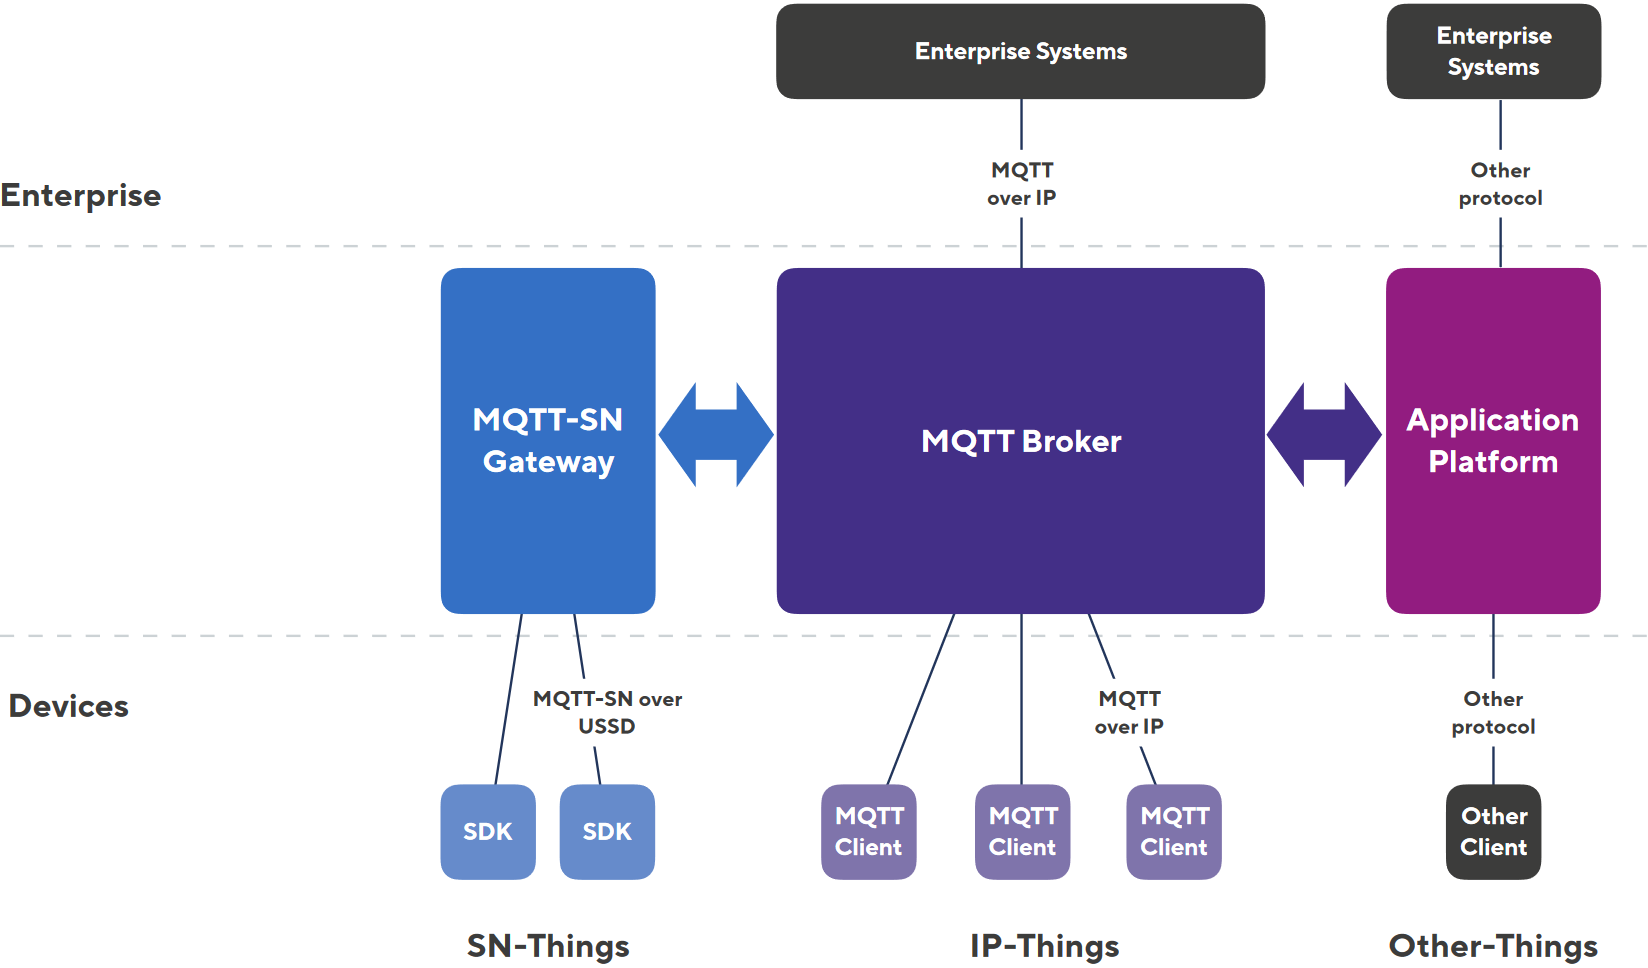
\includegraphics[width=\textwidth]{img/el_prototype/thingstream_archi.png}
  \caption{Architecture simplifiée de la plateforme Thingstream \cite{thing_archi}}
  \label{fig:thing_archi}
\end{figure}
~

\noindent
Plus de détails sur cette fonctionnalité sont disponible sur \cite{thing_dataflow}. Cependant, il est très important de noter que Thingstream offre la possibilité d'envoyer des SMS. De ce fait, les deux types de communication requis pour ce projet sont supportés par Thingstream.

~

\noindent
En résumé, Thingstream offre un service exploitant tous les avantages du protocole USSD, mais sans devoir passer directement par un opérateur. Cependant, l'utilisation de ce service n'est pas sans risque. Toute la partie de communication du projet sera dépendante de cette tierce partie. Par conséquent, si Thingstream, pour une raison quelconque, cesse d'offrir ce service, la partie communication du prototype sera complètement inopérante. De façon à limiter le possible impact de ce risque, des mesures ont été prises lors de la conception de l'architecture de l'application. Ceci sera présenté plus tard dans la section \ref{sec:archi}.

\subsection{Tests réalisés}
\label{sec:prototests}

\noindent
Une fois les principaux composants définis, le prototype a été testé pour s'assurer que tous les composants fonctionnaient correctement ensemble. En outre, il fallait vérifier si le SIM800L fonctionnait correctement avec le SDK de Thingstream, ou s'il causerait les mêmes problèmes que ceux rencontrés l'année précédente. De ce fait, un protocole de test a été mis en place.

~

\noindent
Très brièvement, ce protocole consiste à lancer un stress test sur deux cœurs du CPU du Raspberry Pi et, en même temps, de publier un message toutes les 4 minutes sur un topic MQTT en utilisant le SIM800L et la plateforme Thingstream. Pendant le test, un serveur est aussi connecté à la plateforme de Thingstream (IP-Thing) et son but est de répondre à toute demande envoyée par le Raspberry Pi. Après l'envoi du message, le Raspberry Pi attend pendant maximum 2 minutes la réponse du serveur. Si aucune réponse n'est reçue, l'occurrence est enregistrée sur un fichier .txt. Le diagramme de séquence \ref{fig:dia_test} montre comment fonctionne l'envoi d'un message pendant une expérimentation. Le test a une durée de 4 heures et 45 minutes. Après cette période, des mesures de température supplémentaires sont prises pendant 15 minutes. Ce protocole a été automatisé à l'aide de scripts python afin de garantir sa reproductibilité. Dans l'annexe \ref{ap:teeeest} se trouvent plus de détails concernant le matériel nécessaire, le protocole et la démarche à suivre.

\begin{figure}[ht!]
  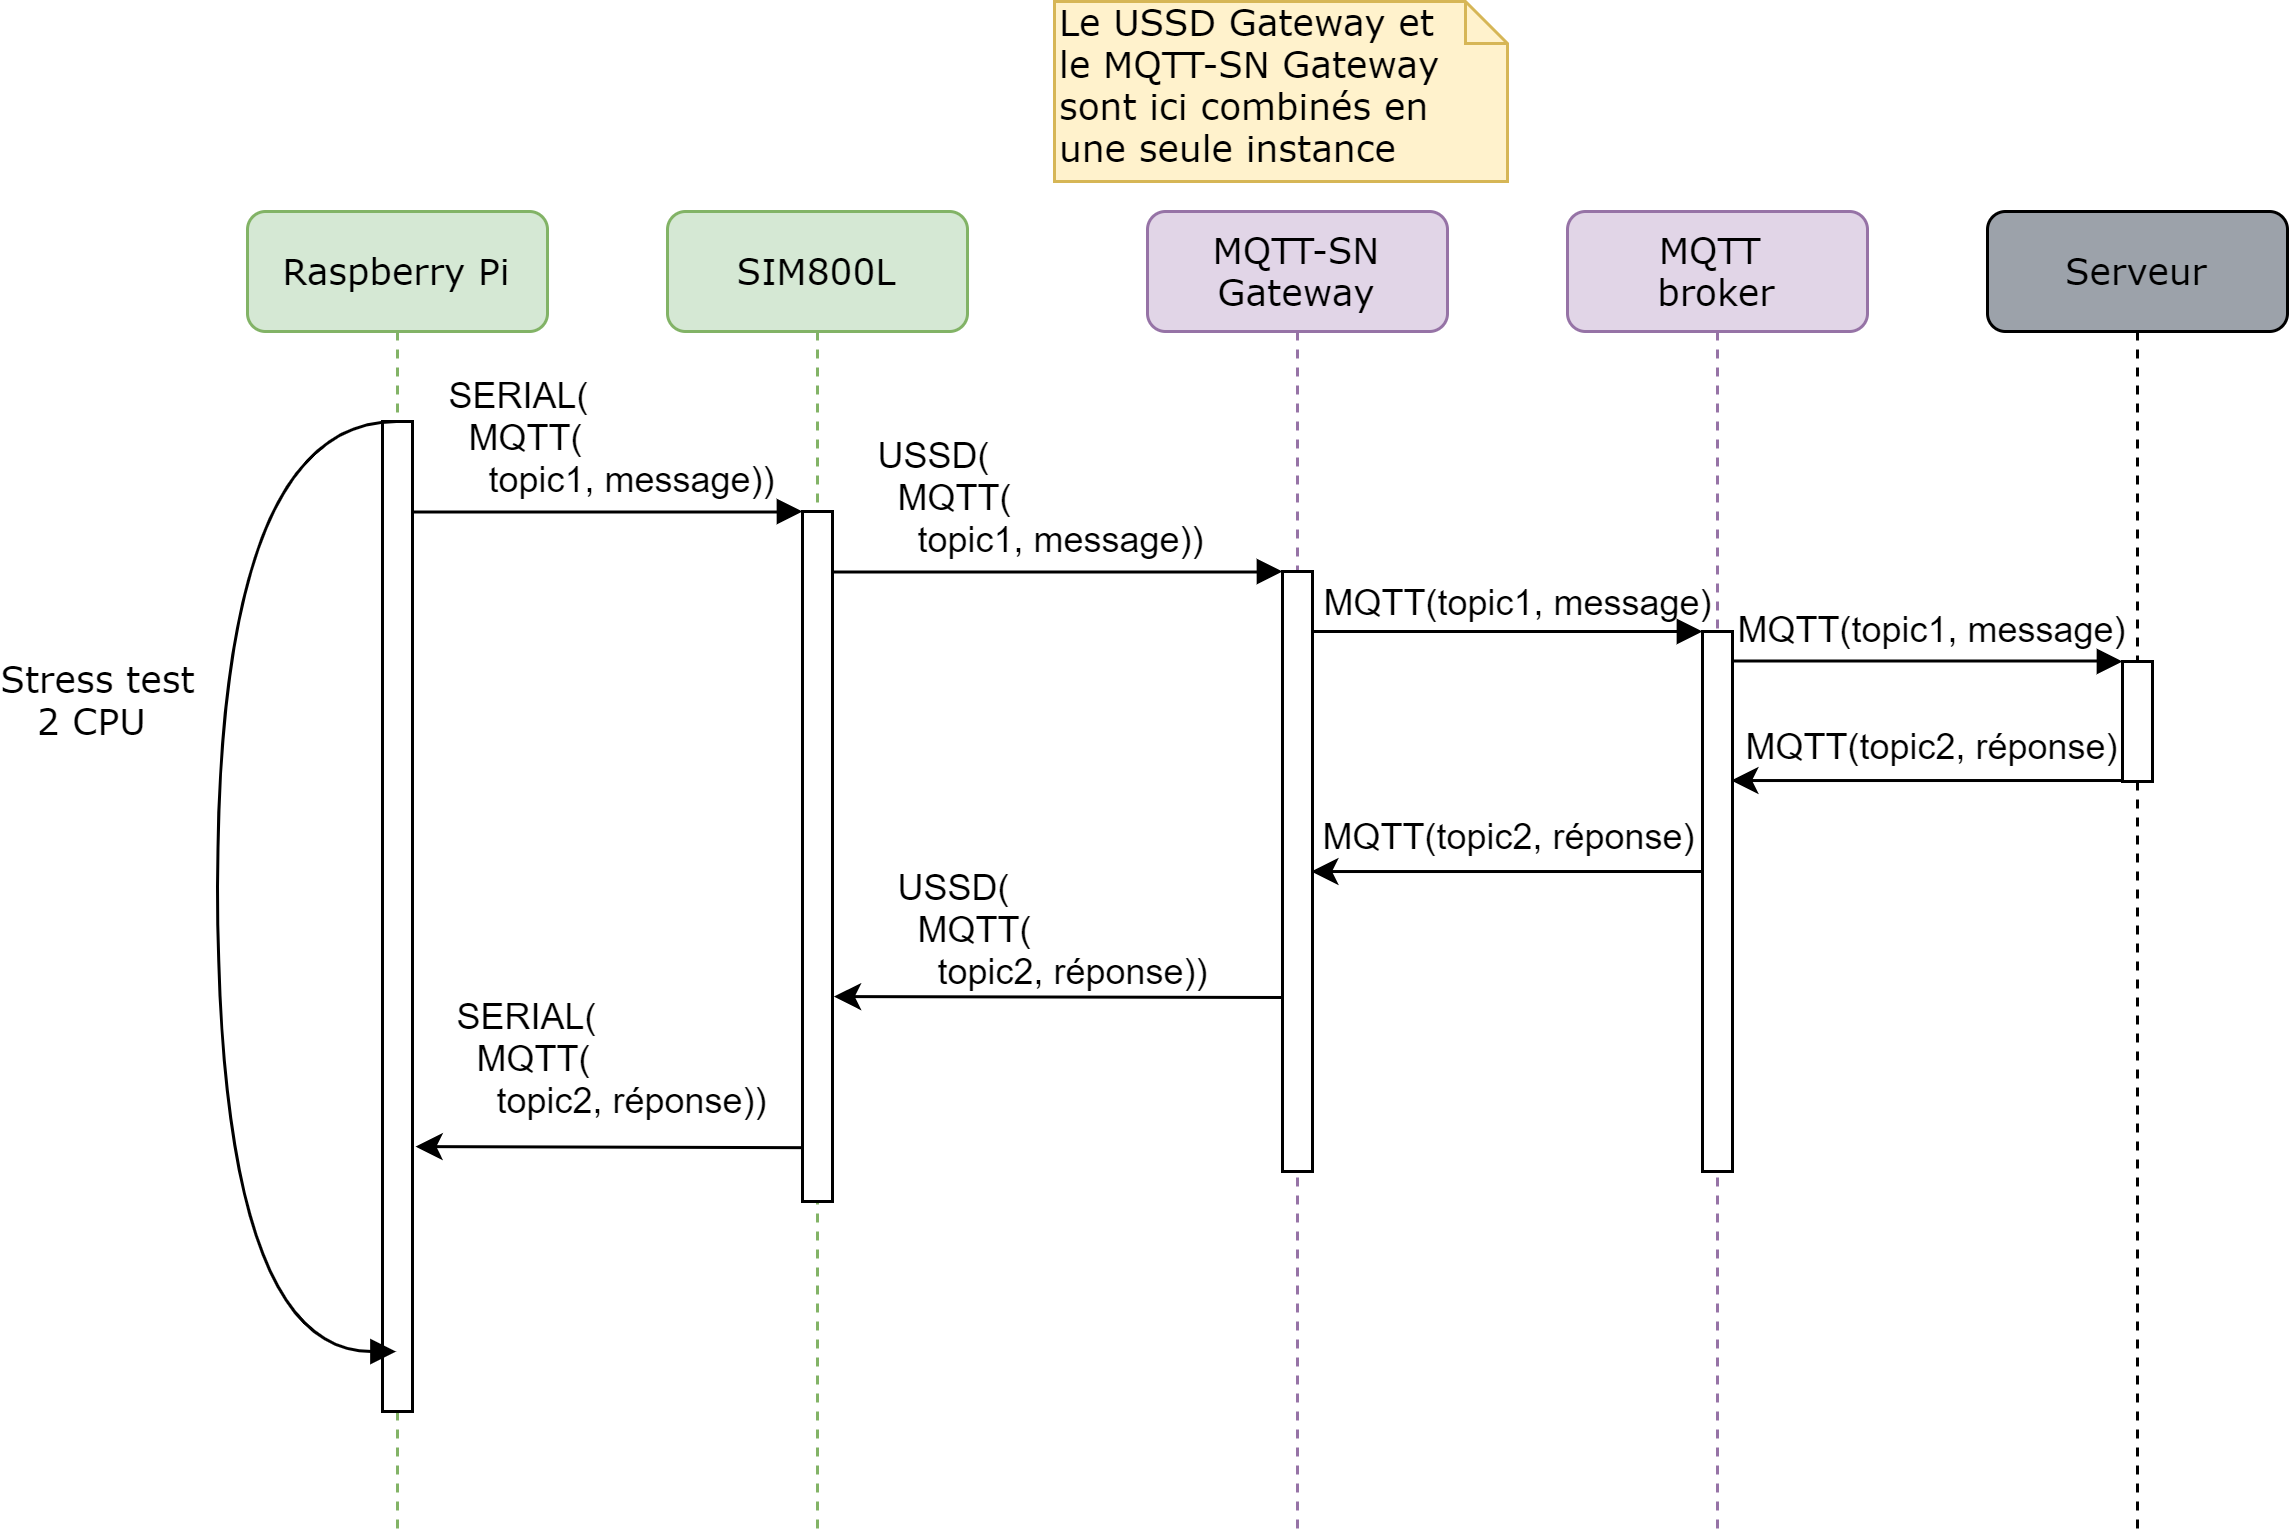
\includegraphics[width=\textwidth]{img/el_prototype/diagram_test.png}
  \caption{Diagramme de séquence de la publication d'un message pendant un test}
  \label{fig:dia_test}
\end{figure}


~

\vspace{-0.5cm}

\noindent
Pendant le test, plusieurs métriques sont surveillées afin d'évaluer le fonctionnement du prototype. En premier lieu, il y a la température du CPU qui est mesurée toutes les 30 secondes. Ensuite, la température de deux zones distinctes est mesurée à l'aide de capteurs externes de température. Ces deux zones sont indiquées sur la figure \ref{fig:dia_test} et correspondent aux deux zones où la température est la plus élevée à l'intérieur du boîtier. Ces trois mesures de température servent principalement à analyser les capacités de refroidissement du boîtier, mais aussi pour vérifier si la température a un impact sur les performances du SIM800L.

\begin{figure}[ht!]
  \centering
  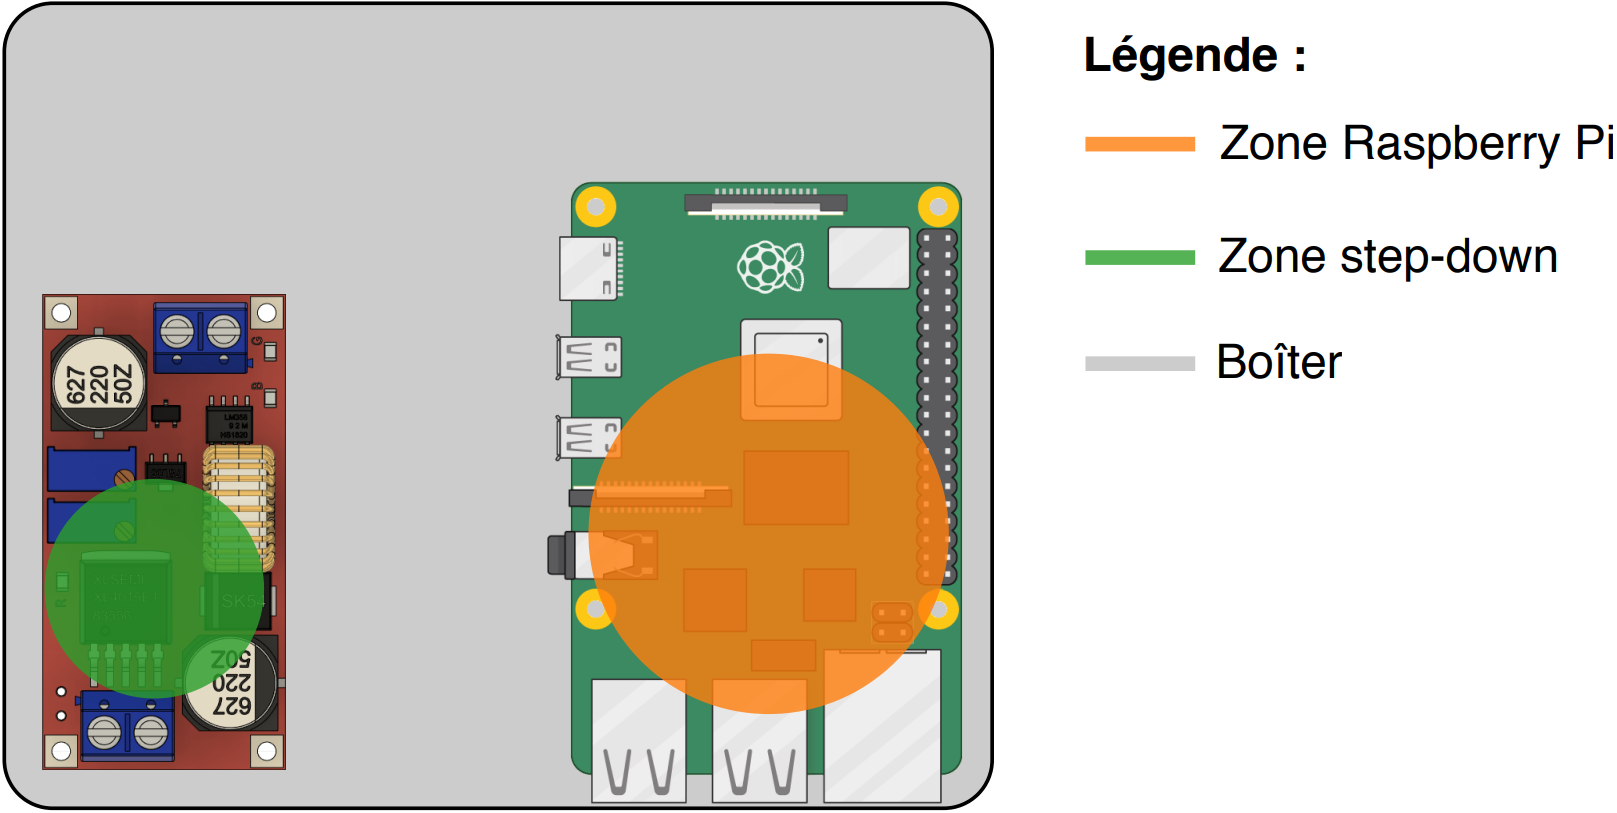
\includegraphics[scale=0.25]{img/el_prototype/zones_temperature.png}
  \caption{Zones où la température a été mesurée lors des tests}
  \label{fig:temp_zones}
\end{figure}

~

\noindent
Ensuite, il y a les métriques liées au fonctionnement du SIM800L.
Les logs produits par le SDK de Thingstream permettent de ressortir deux informations assez importantes : le nombre de messages impossibles à décoder (Receive:parseMessage Warning) et le nombre d'erreurs lors de l'envoi d'un paquet (Protocol:SendPackets Error). La quantité de messages envoyés et reçus par le Raspberry Pi a aussi été enregistrée pour tous les tests, mais cette métrique ne sera pas discutée ici puisque cette valeur était la même pour tous les tests. Toutefois, nous pouvons déjà conclure que le SDK de Thingstream est résilient aux erreurs du modem une fois que le nombre d'erreurs ne semble pas influencer les messages envoyés.

~


\noindent
Les tests présentés ci-dessous ont été réalisés avec le boîtier du prototype de l'année précédente. Le boîtier se trouvait dans une pièce à température contrôlée entre 19,5°C et 20,5°C. Lors de ces tests, le système d'alimentation avec batterie n'a pas utilisé. Au lieu de cela, un chargeur 12V 1.5A DC a été utilisé pour alimenter le XL4015. Chaque test a été répété trois fois et les résultats correspondent à la moyenne de ces trois essais.

~


\noindent
Ce protocole de test a été suivi pour effectuer quatre tests avec des conditions de fonctionnement différentes. Le premier test a été réalisé sans aucun refroidissement actif et avec le step-down à l'intérieur de la boîte. Ce test correspond aux conditions normales de fonctionnement du prototype de l'année dernière.



\begin{figure}[h!]
  \centering
  %% Creator: Matplotlib, PGF backend
%%
%% To include the figure in your LaTeX document, write
%%   \input{<filename>.pgf}
%%
%% Make sure the required packages are loaded in your preamble
%%   \usepackage{pgf}
%%
%% Figures using additional raster images can only be included by \input if
%% they are in the same directory as the main LaTeX file. For loading figures
%% from other directories you can use the `import` package
%%   \usepackage{import}
%% and then include the figures with
%%   \import{<path to file>}{<filename>.pgf}
%%
%% Matplotlib used the following preamble
%%
\begingroup%
\makeatletter%
\begin{pgfpicture}%
\pgfpathrectangle{\pgfpointorigin}{\pgfqpoint{6.400000in}{4.800000in}}%
\pgfusepath{use as bounding box, clip}%
\begin{pgfscope}%
\pgfsetbuttcap%
\pgfsetmiterjoin%
\definecolor{currentfill}{rgb}{1.000000,1.000000,1.000000}%
\pgfsetfillcolor{currentfill}%
\pgfsetlinewidth{0.000000pt}%
\definecolor{currentstroke}{rgb}{1.000000,1.000000,1.000000}%
\pgfsetstrokecolor{currentstroke}%
\pgfsetdash{}{0pt}%
\pgfpathmoveto{\pgfqpoint{0.000000in}{0.000000in}}%
\pgfpathlineto{\pgfqpoint{6.400000in}{0.000000in}}%
\pgfpathlineto{\pgfqpoint{6.400000in}{4.800000in}}%
\pgfpathlineto{\pgfqpoint{0.000000in}{4.800000in}}%
\pgfpathclose%
\pgfusepath{fill}%
\end{pgfscope}%
\begin{pgfscope}%
\pgfsetbuttcap%
\pgfsetmiterjoin%
\definecolor{currentfill}{rgb}{1.000000,1.000000,1.000000}%
\pgfsetfillcolor{currentfill}%
\pgfsetlinewidth{0.000000pt}%
\definecolor{currentstroke}{rgb}{0.000000,0.000000,0.000000}%
\pgfsetstrokecolor{currentstroke}%
\pgfsetstrokeopacity{0.000000}%
\pgfsetdash{}{0pt}%
\pgfpathmoveto{\pgfqpoint{0.800000in}{0.960000in}}%
\pgfpathlineto{\pgfqpoint{5.760000in}{0.960000in}}%
\pgfpathlineto{\pgfqpoint{5.760000in}{4.224000in}}%
\pgfpathlineto{\pgfqpoint{0.800000in}{4.224000in}}%
\pgfpathclose%
\pgfusepath{fill}%
\end{pgfscope}%
\begin{pgfscope}%
\pgfsetbuttcap%
\pgfsetroundjoin%
\definecolor{currentfill}{rgb}{0.000000,0.000000,0.000000}%
\pgfsetfillcolor{currentfill}%
\pgfsetlinewidth{0.803000pt}%
\definecolor{currentstroke}{rgb}{0.000000,0.000000,0.000000}%
\pgfsetstrokecolor{currentstroke}%
\pgfsetdash{}{0pt}%
\pgfsys@defobject{currentmarker}{\pgfqpoint{0.000000in}{-0.048611in}}{\pgfqpoint{0.000000in}{0.000000in}}{%
\pgfpathmoveto{\pgfqpoint{0.000000in}{0.000000in}}%
\pgfpathlineto{\pgfqpoint{0.000000in}{-0.048611in}}%
\pgfusepath{stroke,fill}%
}%
\begin{pgfscope}%
\pgfsys@transformshift{0.800000in}{0.960000in}%
\pgfsys@useobject{currentmarker}{}%
\end{pgfscope}%
\end{pgfscope}%
\begin{pgfscope}%
\definecolor{textcolor}{rgb}{0.000000,0.000000,0.000000}%
\pgfsetstrokecolor{textcolor}%
\pgfsetfillcolor{textcolor}%
\pgftext[x=0.512522in,y=0.621070in,left,base,rotate=30.000000]{\color{textcolor}\rmfamily\fontsize{10.000000}{12.000000}\selectfont 00:00}%
\end{pgfscope}%
\begin{pgfscope}%
\pgfsetbuttcap%
\pgfsetroundjoin%
\definecolor{currentfill}{rgb}{0.000000,0.000000,0.000000}%
\pgfsetfillcolor{currentfill}%
\pgfsetlinewidth{0.803000pt}%
\definecolor{currentstroke}{rgb}{0.000000,0.000000,0.000000}%
\pgfsetstrokecolor{currentstroke}%
\pgfsetdash{}{0pt}%
\pgfsys@defobject{currentmarker}{\pgfqpoint{0.000000in}{-0.048611in}}{\pgfqpoint{0.000000in}{0.000000in}}{%
\pgfpathmoveto{\pgfqpoint{0.000000in}{0.000000in}}%
\pgfpathlineto{\pgfqpoint{0.000000in}{-0.048611in}}%
\pgfusepath{stroke,fill}%
}%
\begin{pgfscope}%
\pgfsys@transformshift{1.791957in}{0.960000in}%
\pgfsys@useobject{currentmarker}{}%
\end{pgfscope}%
\end{pgfscope}%
\begin{pgfscope}%
\definecolor{textcolor}{rgb}{0.000000,0.000000,0.000000}%
\pgfsetstrokecolor{textcolor}%
\pgfsetfillcolor{textcolor}%
\pgftext[x=1.504479in,y=0.621070in,left,base,rotate=30.000000]{\color{textcolor}\rmfamily\fontsize{10.000000}{12.000000}\selectfont 01:00}%
\end{pgfscope}%
\begin{pgfscope}%
\pgfsetbuttcap%
\pgfsetroundjoin%
\definecolor{currentfill}{rgb}{0.000000,0.000000,0.000000}%
\pgfsetfillcolor{currentfill}%
\pgfsetlinewidth{0.803000pt}%
\definecolor{currentstroke}{rgb}{0.000000,0.000000,0.000000}%
\pgfsetstrokecolor{currentstroke}%
\pgfsetdash{}{0pt}%
\pgfsys@defobject{currentmarker}{\pgfqpoint{0.000000in}{-0.048611in}}{\pgfqpoint{0.000000in}{0.000000in}}{%
\pgfpathmoveto{\pgfqpoint{0.000000in}{0.000000in}}%
\pgfpathlineto{\pgfqpoint{0.000000in}{-0.048611in}}%
\pgfusepath{stroke,fill}%
}%
\begin{pgfscope}%
\pgfsys@transformshift{2.783914in}{0.960000in}%
\pgfsys@useobject{currentmarker}{}%
\end{pgfscope}%
\end{pgfscope}%
\begin{pgfscope}%
\definecolor{textcolor}{rgb}{0.000000,0.000000,0.000000}%
\pgfsetstrokecolor{textcolor}%
\pgfsetfillcolor{textcolor}%
\pgftext[x=2.496436in,y=0.621070in,left,base,rotate=30.000000]{\color{textcolor}\rmfamily\fontsize{10.000000}{12.000000}\selectfont 02:00}%
\end{pgfscope}%
\begin{pgfscope}%
\pgfsetbuttcap%
\pgfsetroundjoin%
\definecolor{currentfill}{rgb}{0.000000,0.000000,0.000000}%
\pgfsetfillcolor{currentfill}%
\pgfsetlinewidth{0.803000pt}%
\definecolor{currentstroke}{rgb}{0.000000,0.000000,0.000000}%
\pgfsetstrokecolor{currentstroke}%
\pgfsetdash{}{0pt}%
\pgfsys@defobject{currentmarker}{\pgfqpoint{0.000000in}{-0.048611in}}{\pgfqpoint{0.000000in}{0.000000in}}{%
\pgfpathmoveto{\pgfqpoint{0.000000in}{0.000000in}}%
\pgfpathlineto{\pgfqpoint{0.000000in}{-0.048611in}}%
\pgfusepath{stroke,fill}%
}%
\begin{pgfscope}%
\pgfsys@transformshift{3.775871in}{0.960000in}%
\pgfsys@useobject{currentmarker}{}%
\end{pgfscope}%
\end{pgfscope}%
\begin{pgfscope}%
\definecolor{textcolor}{rgb}{0.000000,0.000000,0.000000}%
\pgfsetstrokecolor{textcolor}%
\pgfsetfillcolor{textcolor}%
\pgftext[x=3.488393in,y=0.621070in,left,base,rotate=30.000000]{\color{textcolor}\rmfamily\fontsize{10.000000}{12.000000}\selectfont 03:00}%
\end{pgfscope}%
\begin{pgfscope}%
\pgfsetbuttcap%
\pgfsetroundjoin%
\definecolor{currentfill}{rgb}{0.000000,0.000000,0.000000}%
\pgfsetfillcolor{currentfill}%
\pgfsetlinewidth{0.803000pt}%
\definecolor{currentstroke}{rgb}{0.000000,0.000000,0.000000}%
\pgfsetstrokecolor{currentstroke}%
\pgfsetdash{}{0pt}%
\pgfsys@defobject{currentmarker}{\pgfqpoint{0.000000in}{-0.048611in}}{\pgfqpoint{0.000000in}{0.000000in}}{%
\pgfpathmoveto{\pgfqpoint{0.000000in}{0.000000in}}%
\pgfpathlineto{\pgfqpoint{0.000000in}{-0.048611in}}%
\pgfusepath{stroke,fill}%
}%
\begin{pgfscope}%
\pgfsys@transformshift{4.767828in}{0.960000in}%
\pgfsys@useobject{currentmarker}{}%
\end{pgfscope}%
\end{pgfscope}%
\begin{pgfscope}%
\definecolor{textcolor}{rgb}{0.000000,0.000000,0.000000}%
\pgfsetstrokecolor{textcolor}%
\pgfsetfillcolor{textcolor}%
\pgftext[x=4.480350in,y=0.621070in,left,base,rotate=30.000000]{\color{textcolor}\rmfamily\fontsize{10.000000}{12.000000}\selectfont 04:00}%
\end{pgfscope}%
\begin{pgfscope}%
\pgfsetbuttcap%
\pgfsetroundjoin%
\definecolor{currentfill}{rgb}{0.000000,0.000000,0.000000}%
\pgfsetfillcolor{currentfill}%
\pgfsetlinewidth{0.803000pt}%
\definecolor{currentstroke}{rgb}{0.000000,0.000000,0.000000}%
\pgfsetstrokecolor{currentstroke}%
\pgfsetdash{}{0pt}%
\pgfsys@defobject{currentmarker}{\pgfqpoint{0.000000in}{-0.048611in}}{\pgfqpoint{0.000000in}{0.000000in}}{%
\pgfpathmoveto{\pgfqpoint{0.000000in}{0.000000in}}%
\pgfpathlineto{\pgfqpoint{0.000000in}{-0.048611in}}%
\pgfusepath{stroke,fill}%
}%
\begin{pgfscope}%
\pgfsys@transformshift{5.759786in}{0.960000in}%
\pgfsys@useobject{currentmarker}{}%
\end{pgfscope}%
\end{pgfscope}%
\begin{pgfscope}%
\definecolor{textcolor}{rgb}{0.000000,0.000000,0.000000}%
\pgfsetstrokecolor{textcolor}%
\pgfsetfillcolor{textcolor}%
\pgftext[x=5.472308in,y=0.621070in,left,base,rotate=30.000000]{\color{textcolor}\rmfamily\fontsize{10.000000}{12.000000}\selectfont 05:00}%
\end{pgfscope}%
\begin{pgfscope}%
\definecolor{textcolor}{rgb}{0.000000,0.000000,0.000000}%
\pgfsetstrokecolor{textcolor}%
\pgfsetfillcolor{textcolor}%
\pgftext[x=3.280000in,y=0.542126in,,top]{\color{textcolor}\rmfamily\fontsize{10.000000}{12.000000}\selectfont Temps (hh:mm)}%
\end{pgfscope}%
\begin{pgfscope}%
\pgfsetbuttcap%
\pgfsetroundjoin%
\definecolor{currentfill}{rgb}{0.000000,0.000000,0.000000}%
\pgfsetfillcolor{currentfill}%
\pgfsetlinewidth{0.803000pt}%
\definecolor{currentstroke}{rgb}{0.000000,0.000000,0.000000}%
\pgfsetstrokecolor{currentstroke}%
\pgfsetdash{}{0pt}%
\pgfsys@defobject{currentmarker}{\pgfqpoint{-0.048611in}{0.000000in}}{\pgfqpoint{0.000000in}{0.000000in}}{%
\pgfpathmoveto{\pgfqpoint{0.000000in}{0.000000in}}%
\pgfpathlineto{\pgfqpoint{-0.048611in}{0.000000in}}%
\pgfusepath{stroke,fill}%
}%
\begin{pgfscope}%
\pgfsys@transformshift{0.800000in}{0.960000in}%
\pgfsys@useobject{currentmarker}{}%
\end{pgfscope}%
\end{pgfscope}%
\begin{pgfscope}%
\definecolor{textcolor}{rgb}{0.000000,0.000000,0.000000}%
\pgfsetstrokecolor{textcolor}%
\pgfsetfillcolor{textcolor}%
\pgftext[x=0.563888in,y=0.911775in,left,base]{\color{textcolor}\rmfamily\fontsize{10.000000}{12.000000}\selectfont \(\displaystyle 20\)}%
\end{pgfscope}%
\begin{pgfscope}%
\pgfsetbuttcap%
\pgfsetroundjoin%
\definecolor{currentfill}{rgb}{0.000000,0.000000,0.000000}%
\pgfsetfillcolor{currentfill}%
\pgfsetlinewidth{0.803000pt}%
\definecolor{currentstroke}{rgb}{0.000000,0.000000,0.000000}%
\pgfsetstrokecolor{currentstroke}%
\pgfsetdash{}{0pt}%
\pgfsys@defobject{currentmarker}{\pgfqpoint{-0.048611in}{0.000000in}}{\pgfqpoint{0.000000in}{0.000000in}}{%
\pgfpathmoveto{\pgfqpoint{0.000000in}{0.000000in}}%
\pgfpathlineto{\pgfqpoint{-0.048611in}{0.000000in}}%
\pgfusepath{stroke,fill}%
}%
\begin{pgfscope}%
\pgfsys@transformshift{0.800000in}{1.426286in}%
\pgfsys@useobject{currentmarker}{}%
\end{pgfscope}%
\end{pgfscope}%
\begin{pgfscope}%
\definecolor{textcolor}{rgb}{0.000000,0.000000,0.000000}%
\pgfsetstrokecolor{textcolor}%
\pgfsetfillcolor{textcolor}%
\pgftext[x=0.563888in,y=1.378060in,left,base]{\color{textcolor}\rmfamily\fontsize{10.000000}{12.000000}\selectfont \(\displaystyle 25\)}%
\end{pgfscope}%
\begin{pgfscope}%
\pgfsetbuttcap%
\pgfsetroundjoin%
\definecolor{currentfill}{rgb}{0.000000,0.000000,0.000000}%
\pgfsetfillcolor{currentfill}%
\pgfsetlinewidth{0.803000pt}%
\definecolor{currentstroke}{rgb}{0.000000,0.000000,0.000000}%
\pgfsetstrokecolor{currentstroke}%
\pgfsetdash{}{0pt}%
\pgfsys@defobject{currentmarker}{\pgfqpoint{-0.048611in}{0.000000in}}{\pgfqpoint{0.000000in}{0.000000in}}{%
\pgfpathmoveto{\pgfqpoint{0.000000in}{0.000000in}}%
\pgfpathlineto{\pgfqpoint{-0.048611in}{0.000000in}}%
\pgfusepath{stroke,fill}%
}%
\begin{pgfscope}%
\pgfsys@transformshift{0.800000in}{1.892571in}%
\pgfsys@useobject{currentmarker}{}%
\end{pgfscope}%
\end{pgfscope}%
\begin{pgfscope}%
\definecolor{textcolor}{rgb}{0.000000,0.000000,0.000000}%
\pgfsetstrokecolor{textcolor}%
\pgfsetfillcolor{textcolor}%
\pgftext[x=0.563888in,y=1.844346in,left,base]{\color{textcolor}\rmfamily\fontsize{10.000000}{12.000000}\selectfont \(\displaystyle 30\)}%
\end{pgfscope}%
\begin{pgfscope}%
\pgfsetbuttcap%
\pgfsetroundjoin%
\definecolor{currentfill}{rgb}{0.000000,0.000000,0.000000}%
\pgfsetfillcolor{currentfill}%
\pgfsetlinewidth{0.803000pt}%
\definecolor{currentstroke}{rgb}{0.000000,0.000000,0.000000}%
\pgfsetstrokecolor{currentstroke}%
\pgfsetdash{}{0pt}%
\pgfsys@defobject{currentmarker}{\pgfqpoint{-0.048611in}{0.000000in}}{\pgfqpoint{0.000000in}{0.000000in}}{%
\pgfpathmoveto{\pgfqpoint{0.000000in}{0.000000in}}%
\pgfpathlineto{\pgfqpoint{-0.048611in}{0.000000in}}%
\pgfusepath{stroke,fill}%
}%
\begin{pgfscope}%
\pgfsys@transformshift{0.800000in}{2.358857in}%
\pgfsys@useobject{currentmarker}{}%
\end{pgfscope}%
\end{pgfscope}%
\begin{pgfscope}%
\definecolor{textcolor}{rgb}{0.000000,0.000000,0.000000}%
\pgfsetstrokecolor{textcolor}%
\pgfsetfillcolor{textcolor}%
\pgftext[x=0.563888in,y=2.310632in,left,base]{\color{textcolor}\rmfamily\fontsize{10.000000}{12.000000}\selectfont \(\displaystyle 35\)}%
\end{pgfscope}%
\begin{pgfscope}%
\pgfsetbuttcap%
\pgfsetroundjoin%
\definecolor{currentfill}{rgb}{0.000000,0.000000,0.000000}%
\pgfsetfillcolor{currentfill}%
\pgfsetlinewidth{0.803000pt}%
\definecolor{currentstroke}{rgb}{0.000000,0.000000,0.000000}%
\pgfsetstrokecolor{currentstroke}%
\pgfsetdash{}{0pt}%
\pgfsys@defobject{currentmarker}{\pgfqpoint{-0.048611in}{0.000000in}}{\pgfqpoint{0.000000in}{0.000000in}}{%
\pgfpathmoveto{\pgfqpoint{0.000000in}{0.000000in}}%
\pgfpathlineto{\pgfqpoint{-0.048611in}{0.000000in}}%
\pgfusepath{stroke,fill}%
}%
\begin{pgfscope}%
\pgfsys@transformshift{0.800000in}{2.825143in}%
\pgfsys@useobject{currentmarker}{}%
\end{pgfscope}%
\end{pgfscope}%
\begin{pgfscope}%
\definecolor{textcolor}{rgb}{0.000000,0.000000,0.000000}%
\pgfsetstrokecolor{textcolor}%
\pgfsetfillcolor{textcolor}%
\pgftext[x=0.563888in,y=2.776918in,left,base]{\color{textcolor}\rmfamily\fontsize{10.000000}{12.000000}\selectfont \(\displaystyle 40\)}%
\end{pgfscope}%
\begin{pgfscope}%
\pgfsetbuttcap%
\pgfsetroundjoin%
\definecolor{currentfill}{rgb}{0.000000,0.000000,0.000000}%
\pgfsetfillcolor{currentfill}%
\pgfsetlinewidth{0.803000pt}%
\definecolor{currentstroke}{rgb}{0.000000,0.000000,0.000000}%
\pgfsetstrokecolor{currentstroke}%
\pgfsetdash{}{0pt}%
\pgfsys@defobject{currentmarker}{\pgfqpoint{-0.048611in}{0.000000in}}{\pgfqpoint{0.000000in}{0.000000in}}{%
\pgfpathmoveto{\pgfqpoint{0.000000in}{0.000000in}}%
\pgfpathlineto{\pgfqpoint{-0.048611in}{0.000000in}}%
\pgfusepath{stroke,fill}%
}%
\begin{pgfscope}%
\pgfsys@transformshift{0.800000in}{3.291429in}%
\pgfsys@useobject{currentmarker}{}%
\end{pgfscope}%
\end{pgfscope}%
\begin{pgfscope}%
\definecolor{textcolor}{rgb}{0.000000,0.000000,0.000000}%
\pgfsetstrokecolor{textcolor}%
\pgfsetfillcolor{textcolor}%
\pgftext[x=0.563888in,y=3.243203in,left,base]{\color{textcolor}\rmfamily\fontsize{10.000000}{12.000000}\selectfont \(\displaystyle 45\)}%
\end{pgfscope}%
\begin{pgfscope}%
\pgfsetbuttcap%
\pgfsetroundjoin%
\definecolor{currentfill}{rgb}{0.000000,0.000000,0.000000}%
\pgfsetfillcolor{currentfill}%
\pgfsetlinewidth{0.803000pt}%
\definecolor{currentstroke}{rgb}{0.000000,0.000000,0.000000}%
\pgfsetstrokecolor{currentstroke}%
\pgfsetdash{}{0pt}%
\pgfsys@defobject{currentmarker}{\pgfqpoint{-0.048611in}{0.000000in}}{\pgfqpoint{0.000000in}{0.000000in}}{%
\pgfpathmoveto{\pgfqpoint{0.000000in}{0.000000in}}%
\pgfpathlineto{\pgfqpoint{-0.048611in}{0.000000in}}%
\pgfusepath{stroke,fill}%
}%
\begin{pgfscope}%
\pgfsys@transformshift{0.800000in}{3.757714in}%
\pgfsys@useobject{currentmarker}{}%
\end{pgfscope}%
\end{pgfscope}%
\begin{pgfscope}%
\definecolor{textcolor}{rgb}{0.000000,0.000000,0.000000}%
\pgfsetstrokecolor{textcolor}%
\pgfsetfillcolor{textcolor}%
\pgftext[x=0.563888in,y=3.709489in,left,base]{\color{textcolor}\rmfamily\fontsize{10.000000}{12.000000}\selectfont \(\displaystyle 50\)}%
\end{pgfscope}%
\begin{pgfscope}%
\pgfsetbuttcap%
\pgfsetroundjoin%
\definecolor{currentfill}{rgb}{0.000000,0.000000,0.000000}%
\pgfsetfillcolor{currentfill}%
\pgfsetlinewidth{0.803000pt}%
\definecolor{currentstroke}{rgb}{0.000000,0.000000,0.000000}%
\pgfsetstrokecolor{currentstroke}%
\pgfsetdash{}{0pt}%
\pgfsys@defobject{currentmarker}{\pgfqpoint{-0.048611in}{0.000000in}}{\pgfqpoint{0.000000in}{0.000000in}}{%
\pgfpathmoveto{\pgfqpoint{0.000000in}{0.000000in}}%
\pgfpathlineto{\pgfqpoint{-0.048611in}{0.000000in}}%
\pgfusepath{stroke,fill}%
}%
\begin{pgfscope}%
\pgfsys@transformshift{0.800000in}{4.224000in}%
\pgfsys@useobject{currentmarker}{}%
\end{pgfscope}%
\end{pgfscope}%
\begin{pgfscope}%
\definecolor{textcolor}{rgb}{0.000000,0.000000,0.000000}%
\pgfsetstrokecolor{textcolor}%
\pgfsetfillcolor{textcolor}%
\pgftext[x=0.563888in,y=4.175775in,left,base]{\color{textcolor}\rmfamily\fontsize{10.000000}{12.000000}\selectfont \(\displaystyle 55\)}%
\end{pgfscope}%
\begin{pgfscope}%
\definecolor{textcolor}{rgb}{0.000000,0.000000,0.000000}%
\pgfsetstrokecolor{textcolor}%
\pgfsetfillcolor{textcolor}%
\pgftext[x=0.508333in,y=2.592000in,,bottom,rotate=90.000000]{\color{textcolor}\rmfamily\fontsize{10.000000}{12.000000}\selectfont Température (\textdegree{}C)}%
\end{pgfscope}%
\begin{pgfscope}%
\pgfpathrectangle{\pgfqpoint{0.800000in}{0.960000in}}{\pgfqpoint{4.960000in}{3.264000in}}%
\pgfusepath{clip}%
\pgfsetrectcap%
\pgfsetroundjoin%
\pgfsetlinewidth{1.505625pt}%
\definecolor{currentstroke}{rgb}{0.121569,0.466667,0.705882}%
\pgfsetstrokecolor{currentstroke}%
\pgfsetdash{}{0pt}%
\pgfpathmoveto{\pgfqpoint{0.800000in}{2.731886in}}%
\pgfpathlineto{\pgfqpoint{0.808310in}{3.184183in}}%
\pgfpathlineto{\pgfqpoint{0.816588in}{3.356709in}}%
\pgfpathlineto{\pgfqpoint{0.824865in}{3.384686in}}%
\pgfpathlineto{\pgfqpoint{0.833142in}{3.435977in}}%
\pgfpathlineto{\pgfqpoint{0.841419in}{3.435977in}}%
\pgfpathlineto{\pgfqpoint{0.849697in}{3.510583in}}%
\pgfpathlineto{\pgfqpoint{0.857974in}{3.510583in}}%
\pgfpathlineto{\pgfqpoint{0.866251in}{3.533897in}}%
\pgfpathlineto{\pgfqpoint{0.874529in}{3.585189in}}%
\pgfpathlineto{\pgfqpoint{0.891084in}{3.585189in}}%
\pgfpathlineto{\pgfqpoint{0.899362in}{3.636480in}}%
\pgfpathlineto{\pgfqpoint{0.907640in}{3.636480in}}%
\pgfpathlineto{\pgfqpoint{0.915918in}{3.659794in}}%
\pgfpathlineto{\pgfqpoint{0.924193in}{3.687771in}}%
\pgfpathlineto{\pgfqpoint{0.932467in}{3.711086in}}%
\pgfpathlineto{\pgfqpoint{0.940742in}{3.711086in}}%
\pgfpathlineto{\pgfqpoint{0.949019in}{3.687771in}}%
\pgfpathlineto{\pgfqpoint{0.957296in}{3.739063in}}%
\pgfpathlineto{\pgfqpoint{0.965574in}{3.687771in}}%
\pgfpathlineto{\pgfqpoint{0.973852in}{3.711086in}}%
\pgfpathlineto{\pgfqpoint{0.982130in}{3.739063in}}%
\pgfpathlineto{\pgfqpoint{0.990408in}{3.687771in}}%
\pgfpathlineto{\pgfqpoint{0.998683in}{3.757714in}}%
\pgfpathlineto{\pgfqpoint{1.006958in}{3.739063in}}%
\pgfpathlineto{\pgfqpoint{1.015230in}{3.785691in}}%
\pgfpathlineto{\pgfqpoint{1.023507in}{3.739063in}}%
\pgfpathlineto{\pgfqpoint{1.031784in}{3.785691in}}%
\pgfpathlineto{\pgfqpoint{1.040062in}{3.762377in}}%
\pgfpathlineto{\pgfqpoint{1.056618in}{3.809006in}}%
\pgfpathlineto{\pgfqpoint{1.073173in}{3.809006in}}%
\pgfpathlineto{\pgfqpoint{1.081451in}{3.832320in}}%
\pgfpathlineto{\pgfqpoint{1.089729in}{3.832320in}}%
\pgfpathlineto{\pgfqpoint{1.098005in}{3.785691in}}%
\pgfpathlineto{\pgfqpoint{1.106283in}{3.832320in}}%
\pgfpathlineto{\pgfqpoint{1.139394in}{3.832320in}}%
\pgfpathlineto{\pgfqpoint{1.147672in}{3.860297in}}%
\pgfpathlineto{\pgfqpoint{1.155944in}{3.860297in}}%
\pgfpathlineto{\pgfqpoint{1.164222in}{3.785691in}}%
\pgfpathlineto{\pgfqpoint{1.172500in}{3.832320in}}%
\pgfpathlineto{\pgfqpoint{1.189052in}{3.888274in}}%
\pgfpathlineto{\pgfqpoint{1.205597in}{3.888274in}}%
\pgfpathlineto{\pgfqpoint{1.213869in}{3.911589in}}%
\pgfpathlineto{\pgfqpoint{1.222142in}{3.832320in}}%
\pgfpathlineto{\pgfqpoint{1.230417in}{3.911589in}}%
\pgfpathlineto{\pgfqpoint{1.238690in}{3.860297in}}%
\pgfpathlineto{\pgfqpoint{1.246967in}{3.888274in}}%
\pgfpathlineto{\pgfqpoint{1.263515in}{3.888274in}}%
\pgfpathlineto{\pgfqpoint{1.271791in}{3.883611in}}%
\pgfpathlineto{\pgfqpoint{1.280068in}{3.939566in}}%
\pgfpathlineto{\pgfqpoint{1.288343in}{3.911589in}}%
\pgfpathlineto{\pgfqpoint{1.296616in}{3.911589in}}%
\pgfpathlineto{\pgfqpoint{1.304889in}{3.934903in}}%
\pgfpathlineto{\pgfqpoint{1.313166in}{3.860297in}}%
\pgfpathlineto{\pgfqpoint{1.321444in}{3.888274in}}%
\pgfpathlineto{\pgfqpoint{1.329715in}{3.911589in}}%
\pgfpathlineto{\pgfqpoint{1.337988in}{3.911589in}}%
\pgfpathlineto{\pgfqpoint{1.346263in}{3.939566in}}%
\pgfpathlineto{\pgfqpoint{1.354535in}{3.911589in}}%
\pgfpathlineto{\pgfqpoint{1.362807in}{3.934903in}}%
\pgfpathlineto{\pgfqpoint{1.379358in}{3.934903in}}%
\pgfpathlineto{\pgfqpoint{1.387635in}{3.911589in}}%
\pgfpathlineto{\pgfqpoint{1.395912in}{3.911589in}}%
\pgfpathlineto{\pgfqpoint{1.404190in}{3.934903in}}%
\pgfpathlineto{\pgfqpoint{1.420744in}{3.934903in}}%
\pgfpathlineto{\pgfqpoint{1.429022in}{3.962880in}}%
\pgfpathlineto{\pgfqpoint{1.437299in}{3.962880in}}%
\pgfpathlineto{\pgfqpoint{1.445569in}{3.934903in}}%
\pgfpathlineto{\pgfqpoint{1.453845in}{3.911589in}}%
\pgfpathlineto{\pgfqpoint{1.462116in}{3.939566in}}%
\pgfpathlineto{\pgfqpoint{1.470390in}{3.934903in}}%
\pgfpathlineto{\pgfqpoint{1.478663in}{3.934903in}}%
\pgfpathlineto{\pgfqpoint{1.486940in}{3.911589in}}%
\pgfpathlineto{\pgfqpoint{1.495218in}{3.934903in}}%
\pgfpathlineto{\pgfqpoint{1.503490in}{3.962880in}}%
\pgfpathlineto{\pgfqpoint{1.511762in}{3.934903in}}%
\pgfpathlineto{\pgfqpoint{1.520036in}{3.934903in}}%
\pgfpathlineto{\pgfqpoint{1.528310in}{3.888274in}}%
\pgfpathlineto{\pgfqpoint{1.536584in}{3.934903in}}%
\pgfpathlineto{\pgfqpoint{1.544861in}{3.911589in}}%
\pgfpathlineto{\pgfqpoint{1.553139in}{3.934903in}}%
\pgfpathlineto{\pgfqpoint{1.561411in}{3.911589in}}%
\pgfpathlineto{\pgfqpoint{1.569684in}{3.934903in}}%
\pgfpathlineto{\pgfqpoint{1.577958in}{3.911589in}}%
\pgfpathlineto{\pgfqpoint{1.586235in}{3.986194in}}%
\pgfpathlineto{\pgfqpoint{1.594505in}{3.962880in}}%
\pgfpathlineto{\pgfqpoint{1.611060in}{3.962880in}}%
\pgfpathlineto{\pgfqpoint{1.619338in}{3.986194in}}%
\pgfpathlineto{\pgfqpoint{1.635894in}{3.939566in}}%
\pgfpathlineto{\pgfqpoint{1.644168in}{3.934903in}}%
\pgfpathlineto{\pgfqpoint{1.652441in}{3.962880in}}%
\pgfpathlineto{\pgfqpoint{1.660718in}{3.986194in}}%
\pgfpathlineto{\pgfqpoint{1.668995in}{3.934903in}}%
\pgfpathlineto{\pgfqpoint{1.677270in}{3.962880in}}%
\pgfpathlineto{\pgfqpoint{1.685550in}{3.934903in}}%
\pgfpathlineto{\pgfqpoint{1.693825in}{3.986194in}}%
\pgfpathlineto{\pgfqpoint{1.702103in}{3.986194in}}%
\pgfpathlineto{\pgfqpoint{1.710375in}{3.962880in}}%
\pgfpathlineto{\pgfqpoint{1.718653in}{3.962880in}}%
\pgfpathlineto{\pgfqpoint{1.726929in}{4.014171in}}%
\pgfpathlineto{\pgfqpoint{1.743485in}{3.864960in}}%
\pgfpathlineto{\pgfqpoint{1.751758in}{3.986194in}}%
\pgfpathlineto{\pgfqpoint{1.760035in}{3.962880in}}%
\pgfpathlineto{\pgfqpoint{1.768312in}{3.986194in}}%
\pgfpathlineto{\pgfqpoint{1.776590in}{3.934903in}}%
\pgfpathlineto{\pgfqpoint{1.784867in}{3.939566in}}%
\pgfpathlineto{\pgfqpoint{1.793144in}{3.934903in}}%
\pgfpathlineto{\pgfqpoint{1.801422in}{3.986194in}}%
\pgfpathlineto{\pgfqpoint{1.809699in}{3.986194in}}%
\pgfpathlineto{\pgfqpoint{1.817977in}{3.934903in}}%
\pgfpathlineto{\pgfqpoint{1.826255in}{3.934903in}}%
\pgfpathlineto{\pgfqpoint{1.834533in}{3.962880in}}%
\pgfpathlineto{\pgfqpoint{1.842808in}{3.934903in}}%
\pgfpathlineto{\pgfqpoint{1.859363in}{3.934903in}}%
\pgfpathlineto{\pgfqpoint{1.867640in}{3.962880in}}%
\pgfpathlineto{\pgfqpoint{1.875917in}{3.962880in}}%
\pgfpathlineto{\pgfqpoint{1.884195in}{3.986194in}}%
\pgfpathlineto{\pgfqpoint{1.892474in}{3.934903in}}%
\pgfpathlineto{\pgfqpoint{1.900749in}{4.014171in}}%
\pgfpathlineto{\pgfqpoint{1.909027in}{4.014171in}}%
\pgfpathlineto{\pgfqpoint{1.917304in}{3.986194in}}%
\pgfpathlineto{\pgfqpoint{1.925581in}{3.986194in}}%
\pgfpathlineto{\pgfqpoint{1.933859in}{4.037486in}}%
\pgfpathlineto{\pgfqpoint{1.942136in}{4.014171in}}%
\pgfpathlineto{\pgfqpoint{1.950412in}{4.037486in}}%
\pgfpathlineto{\pgfqpoint{1.958690in}{3.911589in}}%
\pgfpathlineto{\pgfqpoint{1.966967in}{3.939566in}}%
\pgfpathlineto{\pgfqpoint{1.975244in}{3.990857in}}%
\pgfpathlineto{\pgfqpoint{1.983522in}{4.014171in}}%
\pgfpathlineto{\pgfqpoint{1.991797in}{3.986194in}}%
\pgfpathlineto{\pgfqpoint{2.000074in}{4.014171in}}%
\pgfpathlineto{\pgfqpoint{2.024901in}{4.014171in}}%
\pgfpathlineto{\pgfqpoint{2.033176in}{3.934903in}}%
\pgfpathlineto{\pgfqpoint{2.041449in}{3.962880in}}%
\pgfpathlineto{\pgfqpoint{2.049722in}{3.934903in}}%
\pgfpathlineto{\pgfqpoint{2.057995in}{3.962880in}}%
\pgfpathlineto{\pgfqpoint{2.066270in}{4.037486in}}%
\pgfpathlineto{\pgfqpoint{2.074543in}{4.037486in}}%
\pgfpathlineto{\pgfqpoint{2.082818in}{3.962880in}}%
\pgfpathlineto{\pgfqpoint{2.091095in}{4.037486in}}%
\pgfpathlineto{\pgfqpoint{2.099372in}{3.934903in}}%
\pgfpathlineto{\pgfqpoint{2.107646in}{3.939566in}}%
\pgfpathlineto{\pgfqpoint{2.115924in}{4.014171in}}%
\pgfpathlineto{\pgfqpoint{2.124201in}{4.014171in}}%
\pgfpathlineto{\pgfqpoint{2.132479in}{4.037486in}}%
\pgfpathlineto{\pgfqpoint{2.157309in}{4.037486in}}%
\pgfpathlineto{\pgfqpoint{2.165581in}{4.014171in}}%
\pgfpathlineto{\pgfqpoint{2.173855in}{3.986194in}}%
\pgfpathlineto{\pgfqpoint{2.182128in}{3.986194in}}%
\pgfpathlineto{\pgfqpoint{2.190404in}{4.037486in}}%
\pgfpathlineto{\pgfqpoint{2.215225in}{4.037486in}}%
\pgfpathlineto{\pgfqpoint{2.223497in}{4.014171in}}%
\pgfpathlineto{\pgfqpoint{2.240051in}{4.014171in}}%
\pgfpathlineto{\pgfqpoint{2.248329in}{3.962880in}}%
\pgfpathlineto{\pgfqpoint{2.256606in}{4.014171in}}%
\pgfpathlineto{\pgfqpoint{2.281438in}{4.014171in}}%
\pgfpathlineto{\pgfqpoint{2.289715in}{4.037486in}}%
\pgfpathlineto{\pgfqpoint{2.297993in}{4.014171in}}%
\pgfpathlineto{\pgfqpoint{2.306270in}{4.037486in}}%
\pgfpathlineto{\pgfqpoint{2.314547in}{4.037486in}}%
\pgfpathlineto{\pgfqpoint{2.322825in}{3.962880in}}%
\pgfpathlineto{\pgfqpoint{2.331101in}{3.986194in}}%
\pgfpathlineto{\pgfqpoint{2.339376in}{4.037486in}}%
\pgfpathlineto{\pgfqpoint{2.364208in}{4.037486in}}%
\pgfpathlineto{\pgfqpoint{2.372486in}{4.014171in}}%
\pgfpathlineto{\pgfqpoint{2.380763in}{4.014171in}}%
\pgfpathlineto{\pgfqpoint{2.389037in}{4.037486in}}%
\pgfpathlineto{\pgfqpoint{2.397313in}{3.986194in}}%
\pgfpathlineto{\pgfqpoint{2.405589in}{4.037486in}}%
\pgfpathlineto{\pgfqpoint{2.430422in}{4.037486in}}%
\pgfpathlineto{\pgfqpoint{2.438699in}{4.014171in}}%
\pgfpathlineto{\pgfqpoint{2.446976in}{4.037486in}}%
\pgfpathlineto{\pgfqpoint{2.480071in}{4.037486in}}%
\pgfpathlineto{\pgfqpoint{2.488346in}{4.014171in}}%
\pgfpathlineto{\pgfqpoint{2.496623in}{4.037486in}}%
\pgfpathlineto{\pgfqpoint{2.529712in}{4.037486in}}%
\pgfpathlineto{\pgfqpoint{2.537985in}{3.986194in}}%
\pgfpathlineto{\pgfqpoint{2.546260in}{3.962880in}}%
\pgfpathlineto{\pgfqpoint{2.554532in}{4.037486in}}%
\pgfpathlineto{\pgfqpoint{2.595916in}{4.037486in}}%
\pgfpathlineto{\pgfqpoint{2.604193in}{4.060800in}}%
\pgfpathlineto{\pgfqpoint{2.612467in}{3.986194in}}%
\pgfpathlineto{\pgfqpoint{2.620739in}{3.962880in}}%
\pgfpathlineto{\pgfqpoint{2.629015in}{4.037486in}}%
\pgfpathlineto{\pgfqpoint{2.662119in}{4.037486in}}%
\pgfpathlineto{\pgfqpoint{2.670390in}{4.014171in}}%
\pgfpathlineto{\pgfqpoint{2.678667in}{4.037486in}}%
\pgfpathlineto{\pgfqpoint{2.686945in}{3.911589in}}%
\pgfpathlineto{\pgfqpoint{2.695218in}{4.014171in}}%
\pgfpathlineto{\pgfqpoint{2.703494in}{4.037486in}}%
\pgfpathlineto{\pgfqpoint{2.711771in}{4.014171in}}%
\pgfpathlineto{\pgfqpoint{2.720049in}{4.037486in}}%
\pgfpathlineto{\pgfqpoint{2.728326in}{4.037486in}}%
\pgfpathlineto{\pgfqpoint{2.736603in}{4.060800in}}%
\pgfpathlineto{\pgfqpoint{2.744880in}{4.037486in}}%
\pgfpathlineto{\pgfqpoint{2.753158in}{4.037486in}}%
\pgfpathlineto{\pgfqpoint{2.761435in}{3.962880in}}%
\pgfpathlineto{\pgfqpoint{2.769709in}{4.037486in}}%
\pgfpathlineto{\pgfqpoint{2.786261in}{4.037486in}}%
\pgfpathlineto{\pgfqpoint{2.794533in}{4.014171in}}%
\pgfpathlineto{\pgfqpoint{2.802809in}{4.037486in}}%
\pgfpathlineto{\pgfqpoint{2.811080in}{4.037486in}}%
\pgfpathlineto{\pgfqpoint{2.819358in}{4.014171in}}%
\pgfpathlineto{\pgfqpoint{2.827635in}{4.037486in}}%
\pgfpathlineto{\pgfqpoint{2.835913in}{3.990857in}}%
\pgfpathlineto{\pgfqpoint{2.844189in}{4.037486in}}%
\pgfpathlineto{\pgfqpoint{2.893845in}{4.037486in}}%
\pgfpathlineto{\pgfqpoint{2.902117in}{3.939566in}}%
\pgfpathlineto{\pgfqpoint{2.918671in}{4.037486in}}%
\pgfpathlineto{\pgfqpoint{2.926942in}{4.014171in}}%
\pgfpathlineto{\pgfqpoint{2.935213in}{4.037486in}}%
\pgfpathlineto{\pgfqpoint{2.943489in}{4.037486in}}%
\pgfpathlineto{\pgfqpoint{2.951769in}{4.014171in}}%
\pgfpathlineto{\pgfqpoint{2.960046in}{4.037486in}}%
\pgfpathlineto{\pgfqpoint{2.968324in}{4.037486in}}%
\pgfpathlineto{\pgfqpoint{2.976601in}{3.986194in}}%
\pgfpathlineto{\pgfqpoint{2.984879in}{3.962880in}}%
\pgfpathlineto{\pgfqpoint{2.993152in}{4.037486in}}%
\pgfpathlineto{\pgfqpoint{3.017969in}{4.037486in}}%
\pgfpathlineto{\pgfqpoint{3.026241in}{4.014171in}}%
\pgfpathlineto{\pgfqpoint{3.034513in}{4.037486in}}%
\pgfpathlineto{\pgfqpoint{3.042786in}{4.014171in}}%
\pgfpathlineto{\pgfqpoint{3.051062in}{3.934903in}}%
\pgfpathlineto{\pgfqpoint{3.059334in}{4.037486in}}%
\pgfpathlineto{\pgfqpoint{3.092437in}{4.037486in}}%
\pgfpathlineto{\pgfqpoint{3.100709in}{4.014171in}}%
\pgfpathlineto{\pgfqpoint{3.108982in}{4.037486in}}%
\pgfpathlineto{\pgfqpoint{3.117254in}{4.014171in}}%
\pgfpathlineto{\pgfqpoint{3.125525in}{3.934903in}}%
\pgfpathlineto{\pgfqpoint{3.133804in}{4.037486in}}%
\pgfpathlineto{\pgfqpoint{3.158626in}{4.037486in}}%
\pgfpathlineto{\pgfqpoint{3.166898in}{3.986194in}}%
\pgfpathlineto{\pgfqpoint{3.175171in}{4.037486in}}%
\pgfpathlineto{\pgfqpoint{3.183444in}{4.014171in}}%
\pgfpathlineto{\pgfqpoint{3.191721in}{3.962880in}}%
\pgfpathlineto{\pgfqpoint{3.199998in}{3.934903in}}%
\pgfpathlineto{\pgfqpoint{3.208276in}{3.986194in}}%
\pgfpathlineto{\pgfqpoint{3.216547in}{4.014171in}}%
\pgfpathlineto{\pgfqpoint{3.224825in}{4.037486in}}%
\pgfpathlineto{\pgfqpoint{3.233103in}{4.037486in}}%
\pgfpathlineto{\pgfqpoint{3.241374in}{4.014171in}}%
\pgfpathlineto{\pgfqpoint{3.249652in}{4.037486in}}%
\pgfpathlineto{\pgfqpoint{3.266206in}{3.934903in}}%
\pgfpathlineto{\pgfqpoint{3.274481in}{3.986194in}}%
\pgfpathlineto{\pgfqpoint{3.282757in}{3.934903in}}%
\pgfpathlineto{\pgfqpoint{3.291035in}{4.014171in}}%
\pgfpathlineto{\pgfqpoint{3.299306in}{4.037486in}}%
\pgfpathlineto{\pgfqpoint{3.332409in}{4.037486in}}%
\pgfpathlineto{\pgfqpoint{3.340686in}{3.883611in}}%
\pgfpathlineto{\pgfqpoint{3.348963in}{3.990857in}}%
\pgfpathlineto{\pgfqpoint{3.357240in}{4.037486in}}%
\pgfpathlineto{\pgfqpoint{3.365511in}{4.014171in}}%
\pgfpathlineto{\pgfqpoint{3.373784in}{4.037486in}}%
\pgfpathlineto{\pgfqpoint{3.382060in}{3.962880in}}%
\pgfpathlineto{\pgfqpoint{3.390337in}{4.037486in}}%
\pgfpathlineto{\pgfqpoint{3.398613in}{4.014171in}}%
\pgfpathlineto{\pgfqpoint{3.406888in}{4.014171in}}%
\pgfpathlineto{\pgfqpoint{3.415167in}{3.934903in}}%
\pgfpathlineto{\pgfqpoint{3.423438in}{3.986194in}}%
\pgfpathlineto{\pgfqpoint{3.431714in}{3.986194in}}%
\pgfpathlineto{\pgfqpoint{3.439985in}{4.014171in}}%
\pgfpathlineto{\pgfqpoint{3.448257in}{4.037486in}}%
\pgfpathlineto{\pgfqpoint{3.456536in}{4.037486in}}%
\pgfpathlineto{\pgfqpoint{3.464811in}{3.962880in}}%
\pgfpathlineto{\pgfqpoint{3.473082in}{3.986194in}}%
\pgfpathlineto{\pgfqpoint{3.481361in}{3.934903in}}%
\pgfpathlineto{\pgfqpoint{3.489638in}{3.934903in}}%
\pgfpathlineto{\pgfqpoint{3.497913in}{4.037486in}}%
\pgfpathlineto{\pgfqpoint{3.506186in}{3.962880in}}%
\pgfpathlineto{\pgfqpoint{3.514464in}{3.986194in}}%
\pgfpathlineto{\pgfqpoint{3.522738in}{4.037486in}}%
\pgfpathlineto{\pgfqpoint{3.531009in}{3.986194in}}%
\pgfpathlineto{\pgfqpoint{3.539287in}{3.986194in}}%
\pgfpathlineto{\pgfqpoint{3.547564in}{4.014171in}}%
\pgfpathlineto{\pgfqpoint{3.555842in}{3.962880in}}%
\pgfpathlineto{\pgfqpoint{3.564116in}{3.962880in}}%
\pgfpathlineto{\pgfqpoint{3.572394in}{3.990857in}}%
\pgfpathlineto{\pgfqpoint{3.588948in}{4.037486in}}%
\pgfpathlineto{\pgfqpoint{3.597219in}{4.037486in}}%
\pgfpathlineto{\pgfqpoint{3.605497in}{4.014171in}}%
\pgfpathlineto{\pgfqpoint{3.613775in}{4.037486in}}%
\pgfpathlineto{\pgfqpoint{3.622052in}{3.986194in}}%
\pgfpathlineto{\pgfqpoint{3.630329in}{3.911589in}}%
\pgfpathlineto{\pgfqpoint{3.638607in}{3.986194in}}%
\pgfpathlineto{\pgfqpoint{3.646885in}{3.990857in}}%
\pgfpathlineto{\pgfqpoint{3.655163in}{4.014171in}}%
\pgfpathlineto{\pgfqpoint{3.663433in}{4.014171in}}%
\pgfpathlineto{\pgfqpoint{3.671711in}{3.990857in}}%
\pgfpathlineto{\pgfqpoint{3.679983in}{4.014171in}}%
\pgfpathlineto{\pgfqpoint{3.688259in}{3.962880in}}%
\pgfpathlineto{\pgfqpoint{3.696532in}{3.986194in}}%
\pgfpathlineto{\pgfqpoint{3.704807in}{3.934903in}}%
\pgfpathlineto{\pgfqpoint{3.721361in}{3.990857in}}%
\pgfpathlineto{\pgfqpoint{3.729639in}{4.037486in}}%
\pgfpathlineto{\pgfqpoint{3.746194in}{4.037486in}}%
\pgfpathlineto{\pgfqpoint{3.754471in}{3.986194in}}%
\pgfpathlineto{\pgfqpoint{3.762749in}{4.014171in}}%
\pgfpathlineto{\pgfqpoint{3.771027in}{3.911589in}}%
\pgfpathlineto{\pgfqpoint{3.779303in}{3.939566in}}%
\pgfpathlineto{\pgfqpoint{3.787574in}{4.014171in}}%
\pgfpathlineto{\pgfqpoint{3.795852in}{3.986194in}}%
\pgfpathlineto{\pgfqpoint{3.804130in}{3.986194in}}%
\pgfpathlineto{\pgfqpoint{3.812407in}{4.014171in}}%
\pgfpathlineto{\pgfqpoint{3.820684in}{4.014171in}}%
\pgfpathlineto{\pgfqpoint{3.828963in}{3.986194in}}%
\pgfpathlineto{\pgfqpoint{3.837241in}{3.986194in}}%
\pgfpathlineto{\pgfqpoint{3.845513in}{3.911589in}}%
\pgfpathlineto{\pgfqpoint{3.853792in}{3.962880in}}%
\pgfpathlineto{\pgfqpoint{3.862069in}{3.962880in}}%
\pgfpathlineto{\pgfqpoint{3.870346in}{4.014171in}}%
\pgfpathlineto{\pgfqpoint{3.878622in}{3.986194in}}%
\pgfpathlineto{\pgfqpoint{3.886900in}{4.014171in}}%
\pgfpathlineto{\pgfqpoint{3.895177in}{3.962880in}}%
\pgfpathlineto{\pgfqpoint{3.903450in}{3.986194in}}%
\pgfpathlineto{\pgfqpoint{3.911723in}{3.990857in}}%
\pgfpathlineto{\pgfqpoint{3.919998in}{3.911589in}}%
\pgfpathlineto{\pgfqpoint{3.928274in}{3.962880in}}%
\pgfpathlineto{\pgfqpoint{3.936551in}{3.986194in}}%
\pgfpathlineto{\pgfqpoint{3.944825in}{4.037486in}}%
\pgfpathlineto{\pgfqpoint{3.953098in}{3.986194in}}%
\pgfpathlineto{\pgfqpoint{3.961375in}{3.962880in}}%
\pgfpathlineto{\pgfqpoint{3.969650in}{4.014171in}}%
\pgfpathlineto{\pgfqpoint{3.977925in}{4.014171in}}%
\pgfpathlineto{\pgfqpoint{3.986197in}{3.939566in}}%
\pgfpathlineto{\pgfqpoint{3.994472in}{3.962880in}}%
\pgfpathlineto{\pgfqpoint{4.002748in}{3.990857in}}%
\pgfpathlineto{\pgfqpoint{4.011024in}{4.037486in}}%
\pgfpathlineto{\pgfqpoint{4.019302in}{3.962880in}}%
\pgfpathlineto{\pgfqpoint{4.027580in}{4.014171in}}%
\pgfpathlineto{\pgfqpoint{4.035851in}{3.962880in}}%
\pgfpathlineto{\pgfqpoint{4.044126in}{4.014171in}}%
\pgfpathlineto{\pgfqpoint{4.052401in}{4.014171in}}%
\pgfpathlineto{\pgfqpoint{4.060678in}{4.037486in}}%
\pgfpathlineto{\pgfqpoint{4.068952in}{3.962880in}}%
\pgfpathlineto{\pgfqpoint{4.077229in}{4.014171in}}%
\pgfpathlineto{\pgfqpoint{4.085505in}{4.014171in}}%
\pgfpathlineto{\pgfqpoint{4.093781in}{4.037486in}}%
\pgfpathlineto{\pgfqpoint{4.102056in}{4.014171in}}%
\pgfpathlineto{\pgfqpoint{4.110334in}{4.014171in}}%
\pgfpathlineto{\pgfqpoint{4.118609in}{3.962880in}}%
\pgfpathlineto{\pgfqpoint{4.126887in}{3.986194in}}%
\pgfpathlineto{\pgfqpoint{4.135165in}{3.939566in}}%
\pgfpathlineto{\pgfqpoint{4.143437in}{3.986194in}}%
\pgfpathlineto{\pgfqpoint{4.151715in}{3.986194in}}%
\pgfpathlineto{\pgfqpoint{4.159992in}{4.014171in}}%
\pgfpathlineto{\pgfqpoint{4.168268in}{4.037486in}}%
\pgfpathlineto{\pgfqpoint{4.176539in}{4.014171in}}%
\pgfpathlineto{\pgfqpoint{4.184816in}{4.037486in}}%
\pgfpathlineto{\pgfqpoint{4.193093in}{4.014171in}}%
\pgfpathlineto{\pgfqpoint{4.201366in}{3.986194in}}%
\pgfpathlineto{\pgfqpoint{4.209644in}{3.962880in}}%
\pgfpathlineto{\pgfqpoint{4.217921in}{3.990857in}}%
\pgfpathlineto{\pgfqpoint{4.234471in}{4.037486in}}%
\pgfpathlineto{\pgfqpoint{4.242748in}{4.014171in}}%
\pgfpathlineto{\pgfqpoint{4.251023in}{4.037486in}}%
\pgfpathlineto{\pgfqpoint{4.259298in}{3.990857in}}%
\pgfpathlineto{\pgfqpoint{4.267576in}{4.037486in}}%
\pgfpathlineto{\pgfqpoint{4.275850in}{3.934903in}}%
\pgfpathlineto{\pgfqpoint{4.284126in}{3.990857in}}%
\pgfpathlineto{\pgfqpoint{4.292402in}{4.037486in}}%
\pgfpathlineto{\pgfqpoint{4.300679in}{4.014171in}}%
\pgfpathlineto{\pgfqpoint{4.308956in}{3.986194in}}%
\pgfpathlineto{\pgfqpoint{4.317234in}{4.014171in}}%
\pgfpathlineto{\pgfqpoint{4.325511in}{4.037486in}}%
\pgfpathlineto{\pgfqpoint{4.333789in}{4.014171in}}%
\pgfpathlineto{\pgfqpoint{4.342066in}{4.037486in}}%
\pgfpathlineto{\pgfqpoint{4.350344in}{3.962880in}}%
\pgfpathlineto{\pgfqpoint{4.358622in}{3.934903in}}%
\pgfpathlineto{\pgfqpoint{4.366896in}{4.014171in}}%
\pgfpathlineto{\pgfqpoint{4.375168in}{4.014171in}}%
\pgfpathlineto{\pgfqpoint{4.383440in}{4.037486in}}%
\pgfpathlineto{\pgfqpoint{4.391717in}{4.014171in}}%
\pgfpathlineto{\pgfqpoint{4.399994in}{4.037486in}}%
\pgfpathlineto{\pgfqpoint{4.416549in}{4.037486in}}%
\pgfpathlineto{\pgfqpoint{4.424823in}{3.911589in}}%
\pgfpathlineto{\pgfqpoint{4.433101in}{4.037486in}}%
\pgfpathlineto{\pgfqpoint{4.466206in}{4.037486in}}%
\pgfpathlineto{\pgfqpoint{4.474476in}{4.060800in}}%
\pgfpathlineto{\pgfqpoint{4.482753in}{4.037486in}}%
\pgfpathlineto{\pgfqpoint{4.491024in}{4.037486in}}%
\pgfpathlineto{\pgfqpoint{4.499300in}{4.014171in}}%
\pgfpathlineto{\pgfqpoint{4.507574in}{4.014171in}}%
\pgfpathlineto{\pgfqpoint{4.515845in}{4.037486in}}%
\pgfpathlineto{\pgfqpoint{4.540674in}{4.037486in}}%
\pgfpathlineto{\pgfqpoint{4.548947in}{4.060800in}}%
\pgfpathlineto{\pgfqpoint{4.565489in}{4.014171in}}%
\pgfpathlineto{\pgfqpoint{4.573767in}{3.911589in}}%
\pgfpathlineto{\pgfqpoint{4.582045in}{3.986194in}}%
\pgfpathlineto{\pgfqpoint{4.590323in}{4.037486in}}%
\pgfpathlineto{\pgfqpoint{4.639976in}{4.037486in}}%
\pgfpathlineto{\pgfqpoint{4.648254in}{3.986194in}}%
\pgfpathlineto{\pgfqpoint{4.656525in}{4.037486in}}%
\pgfpathlineto{\pgfqpoint{4.714458in}{4.037486in}}%
\pgfpathlineto{\pgfqpoint{4.722730in}{3.962880in}}%
\pgfpathlineto{\pgfqpoint{4.731008in}{4.014171in}}%
\pgfpathlineto{\pgfqpoint{4.747555in}{4.060800in}}%
\pgfpathlineto{\pgfqpoint{4.755833in}{4.037486in}}%
\pgfpathlineto{\pgfqpoint{4.788937in}{4.037486in}}%
\pgfpathlineto{\pgfqpoint{4.797216in}{4.014171in}}%
\pgfpathlineto{\pgfqpoint{4.805492in}{4.014171in}}%
\pgfpathlineto{\pgfqpoint{4.813769in}{4.037486in}}%
\pgfpathlineto{\pgfqpoint{4.838600in}{4.037486in}}%
\pgfpathlineto{\pgfqpoint{4.846877in}{4.060800in}}%
\pgfpathlineto{\pgfqpoint{4.855153in}{4.037486in}}%
\pgfpathlineto{\pgfqpoint{4.863428in}{3.986194in}}%
\pgfpathlineto{\pgfqpoint{4.871703in}{3.986194in}}%
\pgfpathlineto{\pgfqpoint{4.879980in}{4.037486in}}%
\pgfpathlineto{\pgfqpoint{4.921367in}{4.037486in}}%
\pgfpathlineto{\pgfqpoint{4.929645in}{4.060800in}}%
\pgfpathlineto{\pgfqpoint{4.937922in}{4.014171in}}%
\pgfpathlineto{\pgfqpoint{4.946196in}{4.014171in}}%
\pgfpathlineto{\pgfqpoint{4.954469in}{4.037486in}}%
\pgfpathlineto{\pgfqpoint{4.971022in}{4.037486in}}%
\pgfpathlineto{\pgfqpoint{4.979295in}{4.060800in}}%
\pgfpathlineto{\pgfqpoint{4.995849in}{4.060800in}}%
\pgfpathlineto{\pgfqpoint{5.004127in}{4.037486in}}%
\pgfpathlineto{\pgfqpoint{5.012398in}{3.986194in}}%
\pgfpathlineto{\pgfqpoint{5.020675in}{4.037486in}}%
\pgfpathlineto{\pgfqpoint{5.070325in}{4.037486in}}%
\pgfpathlineto{\pgfqpoint{5.078599in}{3.962880in}}%
\pgfpathlineto{\pgfqpoint{5.086873in}{3.962880in}}%
\pgfpathlineto{\pgfqpoint{5.095147in}{4.037486in}}%
\pgfpathlineto{\pgfqpoint{5.111701in}{4.037486in}}%
\pgfpathlineto{\pgfqpoint{5.119978in}{4.014171in}}%
\pgfpathlineto{\pgfqpoint{5.128253in}{4.037486in}}%
\pgfpathlineto{\pgfqpoint{5.144802in}{4.037486in}}%
\pgfpathlineto{\pgfqpoint{5.153080in}{3.962880in}}%
\pgfpathlineto{\pgfqpoint{5.161357in}{4.014171in}}%
\pgfpathlineto{\pgfqpoint{5.169634in}{4.014171in}}%
\pgfpathlineto{\pgfqpoint{5.177911in}{4.037486in}}%
\pgfpathlineto{\pgfqpoint{5.202738in}{4.037486in}}%
\pgfpathlineto{\pgfqpoint{5.211016in}{4.014171in}}%
\pgfpathlineto{\pgfqpoint{5.219287in}{4.037486in}}%
\pgfpathlineto{\pgfqpoint{5.227565in}{3.986194in}}%
\pgfpathlineto{\pgfqpoint{5.235843in}{4.037486in}}%
\pgfpathlineto{\pgfqpoint{5.244121in}{4.014171in}}%
\pgfpathlineto{\pgfqpoint{5.252399in}{4.060800in}}%
\pgfpathlineto{\pgfqpoint{5.260670in}{4.014171in}}%
\pgfpathlineto{\pgfqpoint{5.268946in}{4.037486in}}%
\pgfpathlineto{\pgfqpoint{5.277223in}{4.037486in}}%
\pgfpathlineto{\pgfqpoint{5.285500in}{4.014171in}}%
\pgfpathlineto{\pgfqpoint{5.293778in}{4.060800in}}%
\pgfpathlineto{\pgfqpoint{5.302050in}{4.009509in}}%
\pgfpathlineto{\pgfqpoint{5.310328in}{4.037486in}}%
\pgfpathlineto{\pgfqpoint{5.318606in}{4.014171in}}%
\pgfpathlineto{\pgfqpoint{5.326878in}{4.014171in}}%
\pgfpathlineto{\pgfqpoint{5.343434in}{4.060800in}}%
\pgfpathlineto{\pgfqpoint{5.351705in}{4.037486in}}%
\pgfpathlineto{\pgfqpoint{5.359981in}{4.060800in}}%
\pgfpathlineto{\pgfqpoint{5.368254in}{3.986194in}}%
\pgfpathlineto{\pgfqpoint{5.376528in}{3.934903in}}%
\pgfpathlineto{\pgfqpoint{5.384803in}{4.037486in}}%
\pgfpathlineto{\pgfqpoint{5.409635in}{4.037486in}}%
\pgfpathlineto{\pgfqpoint{5.417913in}{3.986194in}}%
\pgfpathlineto{\pgfqpoint{5.426191in}{4.037486in}}%
\pgfpathlineto{\pgfqpoint{5.434469in}{4.014171in}}%
\pgfpathlineto{\pgfqpoint{5.442745in}{3.986194in}}%
\pgfpathlineto{\pgfqpoint{5.451023in}{3.986194in}}%
\pgfpathlineto{\pgfqpoint{5.459297in}{4.037486in}}%
\pgfpathlineto{\pgfqpoint{5.467574in}{4.037486in}}%
\pgfpathlineto{\pgfqpoint{5.475851in}{4.014171in}}%
\pgfpathlineto{\pgfqpoint{5.484128in}{4.060800in}}%
\pgfpathlineto{\pgfqpoint{5.492406in}{4.037486in}}%
\pgfpathlineto{\pgfqpoint{5.508960in}{4.037486in}}%
\pgfpathlineto{\pgfqpoint{5.517238in}{3.510583in}}%
\pgfpathlineto{\pgfqpoint{5.533787in}{3.310080in}}%
\pgfpathlineto{\pgfqpoint{5.542066in}{3.282103in}}%
\pgfpathlineto{\pgfqpoint{5.550339in}{3.282103in}}%
\pgfpathlineto{\pgfqpoint{5.566884in}{3.188846in}}%
\pgfpathlineto{\pgfqpoint{5.575156in}{3.184183in}}%
\pgfpathlineto{\pgfqpoint{5.583428in}{3.132891in}}%
\pgfpathlineto{\pgfqpoint{5.591700in}{3.132891in}}%
\pgfpathlineto{\pgfqpoint{5.599972in}{3.109577in}}%
\pgfpathlineto{\pgfqpoint{5.608251in}{3.132891in}}%
\pgfpathlineto{\pgfqpoint{5.616530in}{3.086263in}}%
\pgfpathlineto{\pgfqpoint{5.633088in}{3.086263in}}%
\pgfpathlineto{\pgfqpoint{5.641368in}{3.081600in}}%
\pgfpathlineto{\pgfqpoint{5.649647in}{3.058286in}}%
\pgfpathlineto{\pgfqpoint{5.657926in}{3.058286in}}%
\pgfpathlineto{\pgfqpoint{5.666205in}{3.030309in}}%
\pgfpathlineto{\pgfqpoint{5.674485in}{3.058286in}}%
\pgfpathlineto{\pgfqpoint{5.682764in}{3.058286in}}%
\pgfpathlineto{\pgfqpoint{5.691040in}{3.030309in}}%
\pgfpathlineto{\pgfqpoint{5.715872in}{3.030309in}}%
\pgfpathlineto{\pgfqpoint{5.732421in}{2.983680in}}%
\pgfpathlineto{\pgfqpoint{5.740695in}{3.030309in}}%
\pgfpathlineto{\pgfqpoint{5.748970in}{2.983680in}}%
\pgfpathlineto{\pgfqpoint{5.757245in}{3.030309in}}%
\pgfpathlineto{\pgfqpoint{5.757245in}{3.030309in}}%
\pgfusepath{stroke}%
\end{pgfscope}%
\begin{pgfscope}%
\pgfpathrectangle{\pgfqpoint{0.800000in}{0.960000in}}{\pgfqpoint{4.960000in}{3.264000in}}%
\pgfusepath{clip}%
\pgfsetrectcap%
\pgfsetroundjoin%
\pgfsetlinewidth{1.505625pt}%
\definecolor{currentstroke}{rgb}{1.000000,0.498039,0.054902}%
\pgfsetstrokecolor{currentstroke}%
\pgfsetdash{}{0pt}%
\pgfpathmoveto{\pgfqpoint{0.790000in}{1.624639in}}%
\pgfpathlineto{\pgfqpoint{0.794114in}{1.627371in}}%
\pgfpathlineto{\pgfqpoint{0.802887in}{1.630286in}}%
\pgfpathlineto{\pgfqpoint{0.811661in}{1.639029in}}%
\pgfpathlineto{\pgfqpoint{0.820434in}{1.641943in}}%
\pgfpathlineto{\pgfqpoint{0.829207in}{1.650686in}}%
\pgfpathlineto{\pgfqpoint{0.837980in}{1.653600in}}%
\pgfpathlineto{\pgfqpoint{0.846754in}{1.662343in}}%
\pgfpathlineto{\pgfqpoint{0.864300in}{1.674000in}}%
\pgfpathlineto{\pgfqpoint{0.873074in}{1.682743in}}%
\pgfpathlineto{\pgfqpoint{0.881846in}{1.685657in}}%
\pgfpathlineto{\pgfqpoint{0.890620in}{1.694400in}}%
\pgfpathlineto{\pgfqpoint{0.899394in}{1.700229in}}%
\pgfpathlineto{\pgfqpoint{0.908161in}{1.708971in}}%
\pgfpathlineto{\pgfqpoint{0.916918in}{1.714800in}}%
\pgfpathlineto{\pgfqpoint{0.925692in}{1.723543in}}%
\pgfpathlineto{\pgfqpoint{0.934465in}{1.729371in}}%
\pgfpathlineto{\pgfqpoint{0.943238in}{1.738114in}}%
\pgfpathlineto{\pgfqpoint{0.960785in}{1.749771in}}%
\pgfpathlineto{\pgfqpoint{0.969558in}{1.758514in}}%
\pgfpathlineto{\pgfqpoint{0.978331in}{1.761429in}}%
\pgfpathlineto{\pgfqpoint{1.004651in}{1.778914in}}%
\pgfpathlineto{\pgfqpoint{1.013419in}{1.787657in}}%
\pgfpathlineto{\pgfqpoint{1.022176in}{1.793486in}}%
\pgfpathlineto{\pgfqpoint{1.030943in}{1.796400in}}%
\pgfpathlineto{\pgfqpoint{1.048474in}{1.808057in}}%
\pgfpathlineto{\pgfqpoint{1.057247in}{1.810971in}}%
\pgfpathlineto{\pgfqpoint{1.074794in}{1.822629in}}%
\pgfpathlineto{\pgfqpoint{1.083567in}{1.822629in}}%
\pgfpathlineto{\pgfqpoint{1.101110in}{1.834286in}}%
\pgfpathlineto{\pgfqpoint{1.153754in}{1.851771in}}%
\pgfpathlineto{\pgfqpoint{1.162527in}{1.857600in}}%
\pgfpathlineto{\pgfqpoint{1.171300in}{1.857600in}}%
\pgfpathlineto{\pgfqpoint{1.180073in}{1.863429in}}%
\pgfpathlineto{\pgfqpoint{1.188847in}{1.863429in}}%
\pgfpathlineto{\pgfqpoint{1.215167in}{1.872171in}}%
\pgfpathlineto{\pgfqpoint{1.223934in}{1.872171in}}%
\pgfpathlineto{\pgfqpoint{1.232691in}{1.878000in}}%
\pgfpathlineto{\pgfqpoint{1.250216in}{1.878000in}}%
\pgfpathlineto{\pgfqpoint{1.258989in}{1.883829in}}%
\pgfpathlineto{\pgfqpoint{1.267762in}{1.883829in}}%
\pgfpathlineto{\pgfqpoint{1.294082in}{1.892571in}}%
\pgfpathlineto{\pgfqpoint{1.311626in}{1.892571in}}%
\pgfpathlineto{\pgfqpoint{1.320402in}{1.895486in}}%
\pgfpathlineto{\pgfqpoint{1.329176in}{1.895486in}}%
\pgfpathlineto{\pgfqpoint{1.346722in}{1.901314in}}%
\pgfpathlineto{\pgfqpoint{1.364269in}{1.901314in}}%
\pgfpathlineto{\pgfqpoint{1.381815in}{1.907143in}}%
\pgfpathlineto{\pgfqpoint{1.390589in}{1.907143in}}%
\pgfpathlineto{\pgfqpoint{1.399362in}{1.910057in}}%
\pgfpathlineto{\pgfqpoint{1.416909in}{1.910057in}}%
\pgfpathlineto{\pgfqpoint{1.434449in}{1.915886in}}%
\pgfpathlineto{\pgfqpoint{1.460753in}{1.915886in}}%
\pgfpathlineto{\pgfqpoint{1.469527in}{1.918800in}}%
\pgfpathlineto{\pgfqpoint{1.487073in}{1.918800in}}%
\pgfpathlineto{\pgfqpoint{1.504620in}{1.924629in}}%
\pgfpathlineto{\pgfqpoint{1.530940in}{1.924629in}}%
\pgfpathlineto{\pgfqpoint{1.539707in}{1.927543in}}%
\pgfpathlineto{\pgfqpoint{1.557238in}{1.927543in}}%
\pgfpathlineto{\pgfqpoint{1.566011in}{1.930457in}}%
\pgfpathlineto{\pgfqpoint{1.574784in}{1.930457in}}%
\pgfpathlineto{\pgfqpoint{1.583558in}{1.933371in}}%
\pgfpathlineto{\pgfqpoint{1.618629in}{1.933371in}}%
\pgfpathlineto{\pgfqpoint{1.627399in}{1.936286in}}%
\pgfpathlineto{\pgfqpoint{1.653722in}{1.936286in}}%
\pgfpathlineto{\pgfqpoint{1.662495in}{1.939200in}}%
\pgfpathlineto{\pgfqpoint{1.671269in}{1.936286in}}%
\pgfpathlineto{\pgfqpoint{1.680042in}{1.942114in}}%
\pgfpathlineto{\pgfqpoint{1.723908in}{1.942114in}}%
\pgfpathlineto{\pgfqpoint{1.741455in}{1.947943in}}%
\pgfpathlineto{\pgfqpoint{1.767753in}{1.947943in}}%
\pgfpathlineto{\pgfqpoint{1.776526in}{1.950857in}}%
\pgfpathlineto{\pgfqpoint{1.794073in}{1.950857in}}%
\pgfpathlineto{\pgfqpoint{1.802846in}{1.953771in}}%
\pgfpathlineto{\pgfqpoint{1.811620in}{1.953771in}}%
\pgfpathlineto{\pgfqpoint{1.820393in}{1.956686in}}%
\pgfpathlineto{\pgfqpoint{1.829166in}{1.956686in}}%
\pgfpathlineto{\pgfqpoint{1.837939in}{1.959600in}}%
\pgfpathlineto{\pgfqpoint{1.855480in}{1.959600in}}%
\pgfpathlineto{\pgfqpoint{1.864237in}{1.962514in}}%
\pgfpathlineto{\pgfqpoint{1.881784in}{1.962514in}}%
\pgfpathlineto{\pgfqpoint{1.890557in}{1.965429in}}%
\pgfpathlineto{\pgfqpoint{1.908104in}{1.965429in}}%
\pgfpathlineto{\pgfqpoint{1.925647in}{1.971257in}}%
\pgfpathlineto{\pgfqpoint{1.951970in}{1.971257in}}%
\pgfpathlineto{\pgfqpoint{1.960738in}{1.974171in}}%
\pgfpathlineto{\pgfqpoint{1.978268in}{1.974171in}}%
\pgfpathlineto{\pgfqpoint{1.987042in}{1.980000in}}%
\pgfpathlineto{\pgfqpoint{2.022135in}{1.980000in}}%
\pgfpathlineto{\pgfqpoint{2.030908in}{1.982914in}}%
\pgfpathlineto{\pgfqpoint{2.039681in}{1.982914in}}%
\pgfpathlineto{\pgfqpoint{2.048455in}{1.985829in}}%
\pgfpathlineto{\pgfqpoint{2.057228in}{1.982914in}}%
\pgfpathlineto{\pgfqpoint{2.074753in}{1.988743in}}%
\pgfpathlineto{\pgfqpoint{2.083526in}{1.985829in}}%
\pgfpathlineto{\pgfqpoint{2.092299in}{1.991657in}}%
\pgfpathlineto{\pgfqpoint{2.118619in}{1.991657in}}%
\pgfpathlineto{\pgfqpoint{2.127393in}{1.994571in}}%
\pgfpathlineto{\pgfqpoint{2.144939in}{1.994571in}}%
\pgfpathlineto{\pgfqpoint{2.153712in}{1.997486in}}%
\pgfpathlineto{\pgfqpoint{2.162486in}{1.997486in}}%
\pgfpathlineto{\pgfqpoint{2.171253in}{2.000400in}}%
\pgfpathlineto{\pgfqpoint{2.197533in}{2.000400in}}%
\pgfpathlineto{\pgfqpoint{2.206308in}{2.003314in}}%
\pgfpathlineto{\pgfqpoint{2.232628in}{2.003314in}}%
\pgfpathlineto{\pgfqpoint{2.241401in}{2.006229in}}%
\pgfpathlineto{\pgfqpoint{2.250175in}{2.006229in}}%
\pgfpathlineto{\pgfqpoint{2.258945in}{2.009143in}}%
\pgfpathlineto{\pgfqpoint{2.302815in}{2.009143in}}%
\pgfpathlineto{\pgfqpoint{2.311588in}{2.012057in}}%
\pgfpathlineto{\pgfqpoint{2.337908in}{2.012057in}}%
\pgfpathlineto{\pgfqpoint{2.346681in}{2.014971in}}%
\pgfpathlineto{\pgfqpoint{2.417107in}{2.014971in}}%
\pgfpathlineto{\pgfqpoint{2.425883in}{2.017886in}}%
\pgfpathlineto{\pgfqpoint{2.434657in}{2.017886in}}%
\pgfpathlineto{\pgfqpoint{2.443430in}{2.020800in}}%
\pgfpathlineto{\pgfqpoint{2.452203in}{2.017886in}}%
\pgfpathlineto{\pgfqpoint{2.460977in}{2.020800in}}%
\pgfpathlineto{\pgfqpoint{2.539930in}{2.020800in}}%
\pgfpathlineto{\pgfqpoint{2.548688in}{2.023714in}}%
\pgfpathlineto{\pgfqpoint{2.557461in}{2.020800in}}%
\pgfpathlineto{\pgfqpoint{2.566234in}{2.020800in}}%
\pgfpathlineto{\pgfqpoint{2.575008in}{2.023714in}}%
\pgfpathlineto{\pgfqpoint{2.583781in}{2.020800in}}%
\pgfpathlineto{\pgfqpoint{2.592554in}{2.023714in}}%
\pgfpathlineto{\pgfqpoint{2.601328in}{2.020800in}}%
\pgfpathlineto{\pgfqpoint{2.618874in}{2.020800in}}%
\pgfpathlineto{\pgfqpoint{2.627648in}{2.023714in}}%
\pgfpathlineto{\pgfqpoint{2.636421in}{2.023714in}}%
\pgfpathlineto{\pgfqpoint{2.645188in}{2.026629in}}%
\pgfpathlineto{\pgfqpoint{2.662719in}{2.026629in}}%
\pgfpathlineto{\pgfqpoint{2.671492in}{2.023714in}}%
\pgfpathlineto{\pgfqpoint{2.680265in}{2.026629in}}%
\pgfpathlineto{\pgfqpoint{2.750446in}{2.026629in}}%
\pgfpathlineto{\pgfqpoint{2.759203in}{2.023714in}}%
\pgfpathlineto{\pgfqpoint{2.776750in}{2.029543in}}%
\pgfpathlineto{\pgfqpoint{2.811843in}{2.029543in}}%
\pgfpathlineto{\pgfqpoint{2.820616in}{2.026629in}}%
\pgfpathlineto{\pgfqpoint{2.829389in}{2.029543in}}%
\pgfpathlineto{\pgfqpoint{2.838163in}{2.029543in}}%
\pgfpathlineto{\pgfqpoint{2.846936in}{2.026629in}}%
\pgfpathlineto{\pgfqpoint{2.855703in}{2.029543in}}%
\pgfpathlineto{\pgfqpoint{2.864461in}{2.026629in}}%
\pgfpathlineto{\pgfqpoint{3.013585in}{2.026629in}}%
\pgfpathlineto{\pgfqpoint{3.022358in}{2.023714in}}%
\pgfpathlineto{\pgfqpoint{3.101296in}{2.023714in}}%
\pgfpathlineto{\pgfqpoint{3.110069in}{2.020800in}}%
\pgfpathlineto{\pgfqpoint{3.171476in}{2.020800in}}%
\pgfpathlineto{\pgfqpoint{3.180234in}{2.014971in}}%
\pgfpathlineto{\pgfqpoint{3.189007in}{2.017886in}}%
\pgfpathlineto{\pgfqpoint{3.197780in}{2.014971in}}%
\pgfpathlineto{\pgfqpoint{3.206554in}{2.017886in}}%
\pgfpathlineto{\pgfqpoint{3.215326in}{2.014971in}}%
\pgfpathlineto{\pgfqpoint{3.259194in}{2.014971in}}%
\pgfpathlineto{\pgfqpoint{3.267967in}{2.012057in}}%
\pgfpathlineto{\pgfqpoint{3.285491in}{2.012057in}}%
\pgfpathlineto{\pgfqpoint{3.294265in}{2.009143in}}%
\pgfpathlineto{\pgfqpoint{3.355677in}{2.009143in}}%
\pgfpathlineto{\pgfqpoint{3.364451in}{2.006229in}}%
\pgfpathlineto{\pgfqpoint{3.417069in}{2.006229in}}%
\pgfpathlineto{\pgfqpoint{3.425842in}{2.003314in}}%
\pgfpathlineto{\pgfqpoint{3.460935in}{2.003314in}}%
\pgfpathlineto{\pgfqpoint{3.469709in}{2.000400in}}%
\pgfpathlineto{\pgfqpoint{3.513553in}{2.000400in}}%
\pgfpathlineto{\pgfqpoint{3.522327in}{1.997486in}}%
\pgfpathlineto{\pgfqpoint{3.601287in}{1.997486in}}%
\pgfpathlineto{\pgfqpoint{3.610060in}{1.994571in}}%
\pgfpathlineto{\pgfqpoint{3.618833in}{1.997486in}}%
\pgfpathlineto{\pgfqpoint{3.636380in}{1.991657in}}%
\pgfpathlineto{\pgfqpoint{3.662700in}{1.991657in}}%
\pgfpathlineto{\pgfqpoint{3.671473in}{1.994571in}}%
\pgfpathlineto{\pgfqpoint{3.706566in}{1.994571in}}%
\pgfpathlineto{\pgfqpoint{3.715340in}{1.991657in}}%
\pgfpathlineto{\pgfqpoint{3.724113in}{1.994571in}}%
\pgfpathlineto{\pgfqpoint{3.732886in}{1.991657in}}%
\pgfpathlineto{\pgfqpoint{3.776752in}{1.991657in}}%
\pgfpathlineto{\pgfqpoint{3.785525in}{1.994571in}}%
\pgfpathlineto{\pgfqpoint{3.794299in}{1.991657in}}%
\pgfpathlineto{\pgfqpoint{3.803073in}{1.994571in}}%
\pgfpathlineto{\pgfqpoint{3.811840in}{1.991657in}}%
\pgfpathlineto{\pgfqpoint{3.820597in}{1.994571in}}%
\pgfpathlineto{\pgfqpoint{3.829607in}{1.991657in}}%
\pgfpathlineto{\pgfqpoint{3.838361in}{1.994571in}}%
\pgfpathlineto{\pgfqpoint{3.847138in}{1.991657in}}%
\pgfpathlineto{\pgfqpoint{3.855911in}{1.991657in}}%
\pgfpathlineto{\pgfqpoint{3.864684in}{1.994571in}}%
\pgfpathlineto{\pgfqpoint{3.917324in}{1.994571in}}%
\pgfpathlineto{\pgfqpoint{3.926098in}{1.997486in}}%
\pgfpathlineto{\pgfqpoint{3.969942in}{1.997486in}}%
\pgfpathlineto{\pgfqpoint{3.978715in}{2.000400in}}%
\pgfpathlineto{\pgfqpoint{3.996262in}{2.000400in}}%
\pgfpathlineto{\pgfqpoint{4.005029in}{2.003314in}}%
\pgfpathlineto{\pgfqpoint{4.040106in}{2.003314in}}%
\pgfpathlineto{\pgfqpoint{4.048876in}{2.006229in}}%
\pgfpathlineto{\pgfqpoint{4.083951in}{2.006229in}}%
\pgfpathlineto{\pgfqpoint{4.092724in}{2.009143in}}%
\pgfpathlineto{\pgfqpoint{4.101497in}{2.009143in}}%
\pgfpathlineto{\pgfqpoint{4.110271in}{2.012057in}}%
\pgfpathlineto{\pgfqpoint{4.119044in}{2.012057in}}%
\pgfpathlineto{\pgfqpoint{4.127817in}{2.014971in}}%
\pgfpathlineto{\pgfqpoint{4.162911in}{2.014971in}}%
\pgfpathlineto{\pgfqpoint{4.180457in}{2.020800in}}%
\pgfpathlineto{\pgfqpoint{4.206777in}{2.020800in}}%
\pgfpathlineto{\pgfqpoint{4.215573in}{2.023714in}}%
\pgfpathlineto{\pgfqpoint{4.241892in}{2.023714in}}%
\pgfpathlineto{\pgfqpoint{4.259439in}{2.029543in}}%
\pgfpathlineto{\pgfqpoint{4.294532in}{2.029543in}}%
\pgfpathlineto{\pgfqpoint{4.303306in}{2.032457in}}%
\pgfpathlineto{\pgfqpoint{4.312079in}{2.032457in}}%
\pgfpathlineto{\pgfqpoint{4.320852in}{2.035371in}}%
\pgfpathlineto{\pgfqpoint{4.355942in}{2.035371in}}%
\pgfpathlineto{\pgfqpoint{4.364718in}{2.038286in}}%
\pgfpathlineto{\pgfqpoint{4.382265in}{2.038286in}}%
\pgfpathlineto{\pgfqpoint{4.391033in}{2.041200in}}%
\pgfpathlineto{\pgfqpoint{4.408563in}{2.041200in}}%
\pgfpathlineto{\pgfqpoint{4.417337in}{2.044114in}}%
\pgfpathlineto{\pgfqpoint{4.469976in}{2.044114in}}%
\pgfpathlineto{\pgfqpoint{4.478750in}{2.047029in}}%
\pgfpathlineto{\pgfqpoint{4.505048in}{2.047029in}}%
\pgfpathlineto{\pgfqpoint{4.513821in}{2.049943in}}%
\pgfpathlineto{\pgfqpoint{4.575234in}{2.049943in}}%
\pgfpathlineto{\pgfqpoint{4.584007in}{2.052857in}}%
\pgfpathlineto{\pgfqpoint{4.636647in}{2.052857in}}%
\pgfpathlineto{\pgfqpoint{4.645421in}{2.055771in}}%
\pgfpathlineto{\pgfqpoint{4.654194in}{2.052857in}}%
\pgfpathlineto{\pgfqpoint{4.662967in}{2.052857in}}%
\pgfpathlineto{\pgfqpoint{4.671740in}{2.055771in}}%
\pgfpathlineto{\pgfqpoint{4.750943in}{2.055771in}}%
\pgfpathlineto{\pgfqpoint{4.759716in}{2.058686in}}%
\pgfpathlineto{\pgfqpoint{4.856200in}{2.058686in}}%
\pgfpathlineto{\pgfqpoint{4.864974in}{2.055771in}}%
\pgfpathlineto{\pgfqpoint{4.873747in}{2.058686in}}%
\pgfpathlineto{\pgfqpoint{4.952707in}{2.058686in}}%
\pgfpathlineto{\pgfqpoint{4.961480in}{2.055771in}}%
\pgfpathlineto{\pgfqpoint{4.970253in}{2.058686in}}%
\pgfpathlineto{\pgfqpoint{4.987800in}{2.058686in}}%
\pgfpathlineto{\pgfqpoint{4.996573in}{2.055771in}}%
\pgfpathlineto{\pgfqpoint{5.040462in}{2.055771in}}%
\pgfpathlineto{\pgfqpoint{5.049235in}{2.052857in}}%
\pgfpathlineto{\pgfqpoint{5.058009in}{2.055771in}}%
\pgfpathlineto{\pgfqpoint{5.145742in}{2.055771in}}%
\pgfpathlineto{\pgfqpoint{5.154515in}{2.052857in}}%
\pgfpathlineto{\pgfqpoint{5.163288in}{2.052857in}}%
\pgfpathlineto{\pgfqpoint{5.172084in}{2.055771in}}%
\pgfpathlineto{\pgfqpoint{5.180857in}{2.049943in}}%
\pgfpathlineto{\pgfqpoint{5.189630in}{2.055771in}}%
\pgfpathlineto{\pgfqpoint{5.207177in}{2.049943in}}%
\pgfpathlineto{\pgfqpoint{5.365339in}{2.049943in}}%
\pgfpathlineto{\pgfqpoint{5.374112in}{2.047029in}}%
\pgfpathlineto{\pgfqpoint{5.382885in}{2.049943in}}%
\pgfpathlineto{\pgfqpoint{5.391659in}{2.049943in}}%
\pgfpathlineto{\pgfqpoint{5.400432in}{2.044114in}}%
\pgfpathlineto{\pgfqpoint{5.496917in}{2.044114in}}%
\pgfpathlineto{\pgfqpoint{5.505690in}{2.041200in}}%
\pgfpathlineto{\pgfqpoint{5.523236in}{2.041200in}}%
\pgfpathlineto{\pgfqpoint{5.532010in}{2.038286in}}%
\pgfpathlineto{\pgfqpoint{5.540783in}{2.038286in}}%
\pgfpathlineto{\pgfqpoint{5.584628in}{2.023714in}}%
\pgfpathlineto{\pgfqpoint{5.602174in}{2.012057in}}%
\pgfpathlineto{\pgfqpoint{5.619721in}{2.006229in}}%
\pgfpathlineto{\pgfqpoint{5.646040in}{1.988743in}}%
\pgfpathlineto{\pgfqpoint{5.654813in}{1.985829in}}%
\pgfpathlineto{\pgfqpoint{5.663587in}{1.977086in}}%
\pgfpathlineto{\pgfqpoint{5.672361in}{1.977086in}}%
\pgfpathlineto{\pgfqpoint{5.707432in}{1.953771in}}%
\pgfpathlineto{\pgfqpoint{5.724978in}{1.947943in}}%
\pgfpathlineto{\pgfqpoint{5.742525in}{1.936286in}}%
\pgfpathlineto{\pgfqpoint{5.751298in}{1.936286in}}%
\pgfpathlineto{\pgfqpoint{5.760071in}{1.930457in}}%
\pgfpathlineto{\pgfqpoint{5.770000in}{1.927159in}}%
\pgfpathlineto{\pgfqpoint{5.770000in}{1.927159in}}%
\pgfusepath{stroke}%
\end{pgfscope}%
\begin{pgfscope}%
\pgfpathrectangle{\pgfqpoint{0.800000in}{0.960000in}}{\pgfqpoint{4.960000in}{3.264000in}}%
\pgfusepath{clip}%
\pgfsetrectcap%
\pgfsetroundjoin%
\pgfsetlinewidth{1.505625pt}%
\definecolor{currentstroke}{rgb}{0.172549,0.627451,0.172549}%
\pgfsetstrokecolor{currentstroke}%
\pgfsetdash{}{0pt}%
\pgfpathmoveto{\pgfqpoint{0.790000in}{1.261720in}}%
\pgfpathlineto{\pgfqpoint{0.794114in}{1.263086in}}%
\pgfpathlineto{\pgfqpoint{0.802887in}{1.260171in}}%
\pgfpathlineto{\pgfqpoint{0.811661in}{1.263086in}}%
\pgfpathlineto{\pgfqpoint{0.837980in}{1.263086in}}%
\pgfpathlineto{\pgfqpoint{0.846754in}{1.266000in}}%
\pgfpathlineto{\pgfqpoint{0.864300in}{1.266000in}}%
\pgfpathlineto{\pgfqpoint{0.873074in}{1.271829in}}%
\pgfpathlineto{\pgfqpoint{0.881846in}{1.271829in}}%
\pgfpathlineto{\pgfqpoint{0.890620in}{1.274743in}}%
\pgfpathlineto{\pgfqpoint{0.908161in}{1.274743in}}%
\pgfpathlineto{\pgfqpoint{0.925692in}{1.280571in}}%
\pgfpathlineto{\pgfqpoint{0.943238in}{1.280571in}}%
\pgfpathlineto{\pgfqpoint{0.952011in}{1.286400in}}%
\pgfpathlineto{\pgfqpoint{0.960785in}{1.289314in}}%
\pgfpathlineto{\pgfqpoint{0.978331in}{1.289314in}}%
\pgfpathlineto{\pgfqpoint{0.987104in}{1.295143in}}%
\pgfpathlineto{\pgfqpoint{1.013419in}{1.295143in}}%
\pgfpathlineto{\pgfqpoint{1.022176in}{1.300971in}}%
\pgfpathlineto{\pgfqpoint{1.048474in}{1.300971in}}%
\pgfpathlineto{\pgfqpoint{1.057247in}{1.306800in}}%
\pgfpathlineto{\pgfqpoint{1.083567in}{1.306800in}}%
\pgfpathlineto{\pgfqpoint{1.101110in}{1.312629in}}%
\pgfpathlineto{\pgfqpoint{1.109887in}{1.312629in}}%
\pgfpathlineto{\pgfqpoint{1.118660in}{1.315543in}}%
\pgfpathlineto{\pgfqpoint{1.144980in}{1.315543in}}%
\pgfpathlineto{\pgfqpoint{1.153754in}{1.321371in}}%
\pgfpathlineto{\pgfqpoint{1.171300in}{1.321371in}}%
\pgfpathlineto{\pgfqpoint{1.180073in}{1.324286in}}%
\pgfpathlineto{\pgfqpoint{1.188847in}{1.324286in}}%
\pgfpathlineto{\pgfqpoint{1.197620in}{1.327200in}}%
\pgfpathlineto{\pgfqpoint{1.206393in}{1.327200in}}%
\pgfpathlineto{\pgfqpoint{1.215167in}{1.330114in}}%
\pgfpathlineto{\pgfqpoint{1.258989in}{1.330114in}}%
\pgfpathlineto{\pgfqpoint{1.267762in}{1.333029in}}%
\pgfpathlineto{\pgfqpoint{1.276536in}{1.333029in}}%
\pgfpathlineto{\pgfqpoint{1.285309in}{1.335943in}}%
\pgfpathlineto{\pgfqpoint{1.311626in}{1.335943in}}%
\pgfpathlineto{\pgfqpoint{1.320402in}{1.341771in}}%
\pgfpathlineto{\pgfqpoint{1.329176in}{1.341771in}}%
\pgfpathlineto{\pgfqpoint{1.337949in}{1.338857in}}%
\pgfpathlineto{\pgfqpoint{1.346722in}{1.341771in}}%
\pgfpathlineto{\pgfqpoint{1.399362in}{1.341771in}}%
\pgfpathlineto{\pgfqpoint{1.408135in}{1.344686in}}%
\pgfpathlineto{\pgfqpoint{1.416909in}{1.341771in}}%
\pgfpathlineto{\pgfqpoint{1.425682in}{1.341771in}}%
\pgfpathlineto{\pgfqpoint{1.434449in}{1.344686in}}%
\pgfpathlineto{\pgfqpoint{1.504620in}{1.344686in}}%
\pgfpathlineto{\pgfqpoint{1.513393in}{1.347600in}}%
\pgfpathlineto{\pgfqpoint{1.601098in}{1.347600in}}%
\pgfpathlineto{\pgfqpoint{1.609855in}{1.350514in}}%
\pgfpathlineto{\pgfqpoint{1.618629in}{1.350514in}}%
\pgfpathlineto{\pgfqpoint{1.627399in}{1.353429in}}%
\pgfpathlineto{\pgfqpoint{1.671269in}{1.353429in}}%
\pgfpathlineto{\pgfqpoint{1.680042in}{1.356343in}}%
\pgfpathlineto{\pgfqpoint{1.715135in}{1.356343in}}%
\pgfpathlineto{\pgfqpoint{1.723908in}{1.359257in}}%
\pgfpathlineto{\pgfqpoint{1.732682in}{1.359257in}}%
\pgfpathlineto{\pgfqpoint{1.741455in}{1.362171in}}%
\pgfpathlineto{\pgfqpoint{1.758980in}{1.362171in}}%
\pgfpathlineto{\pgfqpoint{1.767753in}{1.365086in}}%
\pgfpathlineto{\pgfqpoint{1.785300in}{1.365086in}}%
\pgfpathlineto{\pgfqpoint{1.794073in}{1.368000in}}%
\pgfpathlineto{\pgfqpoint{1.820393in}{1.368000in}}%
\pgfpathlineto{\pgfqpoint{1.829166in}{1.373829in}}%
\pgfpathlineto{\pgfqpoint{1.837939in}{1.373829in}}%
\pgfpathlineto{\pgfqpoint{1.846713in}{1.376743in}}%
\pgfpathlineto{\pgfqpoint{1.855480in}{1.373829in}}%
\pgfpathlineto{\pgfqpoint{1.864237in}{1.373829in}}%
\pgfpathlineto{\pgfqpoint{1.873011in}{1.376743in}}%
\pgfpathlineto{\pgfqpoint{1.899331in}{1.376743in}}%
\pgfpathlineto{\pgfqpoint{1.908104in}{1.379657in}}%
\pgfpathlineto{\pgfqpoint{1.925647in}{1.379657in}}%
\pgfpathlineto{\pgfqpoint{1.934423in}{1.382571in}}%
\pgfpathlineto{\pgfqpoint{1.951970in}{1.382571in}}%
\pgfpathlineto{\pgfqpoint{1.960738in}{1.385486in}}%
\pgfpathlineto{\pgfqpoint{1.978268in}{1.385486in}}%
\pgfpathlineto{\pgfqpoint{1.987042in}{1.388400in}}%
\pgfpathlineto{\pgfqpoint{1.995815in}{1.388400in}}%
\pgfpathlineto{\pgfqpoint{2.004588in}{1.385486in}}%
\pgfpathlineto{\pgfqpoint{2.013362in}{1.391314in}}%
\pgfpathlineto{\pgfqpoint{2.022135in}{1.388400in}}%
\pgfpathlineto{\pgfqpoint{2.030908in}{1.388400in}}%
\pgfpathlineto{\pgfqpoint{2.039681in}{1.394229in}}%
\pgfpathlineto{\pgfqpoint{2.048455in}{1.391314in}}%
\pgfpathlineto{\pgfqpoint{2.057228in}{1.391314in}}%
\pgfpathlineto{\pgfqpoint{2.065995in}{1.394229in}}%
\pgfpathlineto{\pgfqpoint{2.083526in}{1.394229in}}%
\pgfpathlineto{\pgfqpoint{2.092299in}{1.397143in}}%
\pgfpathlineto{\pgfqpoint{2.118619in}{1.397143in}}%
\pgfpathlineto{\pgfqpoint{2.127393in}{1.400057in}}%
\pgfpathlineto{\pgfqpoint{2.162486in}{1.400057in}}%
\pgfpathlineto{\pgfqpoint{2.171253in}{1.402971in}}%
\pgfpathlineto{\pgfqpoint{2.197533in}{1.402971in}}%
\pgfpathlineto{\pgfqpoint{2.206308in}{1.400057in}}%
\pgfpathlineto{\pgfqpoint{2.276495in}{1.400057in}}%
\pgfpathlineto{\pgfqpoint{2.285268in}{1.402971in}}%
\pgfpathlineto{\pgfqpoint{2.294041in}{1.400057in}}%
\pgfpathlineto{\pgfqpoint{2.478523in}{1.400057in}}%
\pgfpathlineto{\pgfqpoint{2.487297in}{1.405886in}}%
\pgfpathlineto{\pgfqpoint{2.496070in}{1.405886in}}%
\pgfpathlineto{\pgfqpoint{2.504843in}{1.402971in}}%
\pgfpathlineto{\pgfqpoint{2.513616in}{1.405886in}}%
\pgfpathlineto{\pgfqpoint{2.531163in}{1.400057in}}%
\pgfpathlineto{\pgfqpoint{2.539930in}{1.402971in}}%
\pgfpathlineto{\pgfqpoint{2.548688in}{1.402971in}}%
\pgfpathlineto{\pgfqpoint{2.557461in}{1.400057in}}%
\pgfpathlineto{\pgfqpoint{2.627648in}{1.400057in}}%
\pgfpathlineto{\pgfqpoint{2.636421in}{1.397143in}}%
\pgfpathlineto{\pgfqpoint{2.653945in}{1.397143in}}%
\pgfpathlineto{\pgfqpoint{2.662719in}{1.394229in}}%
\pgfpathlineto{\pgfqpoint{2.689039in}{1.394229in}}%
\pgfpathlineto{\pgfqpoint{2.697812in}{1.397143in}}%
\pgfpathlineto{\pgfqpoint{2.706585in}{1.394229in}}%
\pgfpathlineto{\pgfqpoint{2.741679in}{1.394229in}}%
\pgfpathlineto{\pgfqpoint{2.750446in}{1.391314in}}%
\pgfpathlineto{\pgfqpoint{2.829389in}{1.391314in}}%
\pgfpathlineto{\pgfqpoint{2.838163in}{1.388400in}}%
\pgfpathlineto{\pgfqpoint{2.846936in}{1.391314in}}%
\pgfpathlineto{\pgfqpoint{2.855703in}{1.388400in}}%
\pgfpathlineto{\pgfqpoint{2.960961in}{1.388400in}}%
\pgfpathlineto{\pgfqpoint{2.969718in}{1.385486in}}%
\pgfpathlineto{\pgfqpoint{2.996038in}{1.385486in}}%
\pgfpathlineto{\pgfqpoint{3.004812in}{1.382571in}}%
\pgfpathlineto{\pgfqpoint{3.048678in}{1.382571in}}%
\pgfpathlineto{\pgfqpoint{3.057452in}{1.379657in}}%
\pgfpathlineto{\pgfqpoint{3.066219in}{1.379657in}}%
\pgfpathlineto{\pgfqpoint{3.074975in}{1.376743in}}%
\pgfpathlineto{\pgfqpoint{3.110069in}{1.376743in}}%
\pgfpathlineto{\pgfqpoint{3.118843in}{1.373829in}}%
\pgfpathlineto{\pgfqpoint{3.145162in}{1.373829in}}%
\pgfpathlineto{\pgfqpoint{3.153936in}{1.370914in}}%
\pgfpathlineto{\pgfqpoint{3.162709in}{1.370914in}}%
\pgfpathlineto{\pgfqpoint{3.171476in}{1.368000in}}%
\pgfpathlineto{\pgfqpoint{3.206554in}{1.368000in}}%
\pgfpathlineto{\pgfqpoint{3.215326in}{1.365086in}}%
\pgfpathlineto{\pgfqpoint{3.224100in}{1.365086in}}%
\pgfpathlineto{\pgfqpoint{3.232874in}{1.362171in}}%
\pgfpathlineto{\pgfqpoint{3.241647in}{1.365086in}}%
\pgfpathlineto{\pgfqpoint{3.250420in}{1.362171in}}%
\pgfpathlineto{\pgfqpoint{3.267967in}{1.362171in}}%
\pgfpathlineto{\pgfqpoint{3.276734in}{1.359257in}}%
\pgfpathlineto{\pgfqpoint{3.320585in}{1.359257in}}%
\pgfpathlineto{\pgfqpoint{3.338131in}{1.353429in}}%
\pgfpathlineto{\pgfqpoint{3.355677in}{1.353429in}}%
\pgfpathlineto{\pgfqpoint{3.364451in}{1.350514in}}%
\pgfpathlineto{\pgfqpoint{3.399522in}{1.350514in}}%
\pgfpathlineto{\pgfqpoint{3.408296in}{1.347600in}}%
\pgfpathlineto{\pgfqpoint{3.460935in}{1.347600in}}%
\pgfpathlineto{\pgfqpoint{3.469709in}{1.344686in}}%
\pgfpathlineto{\pgfqpoint{3.478482in}{1.344686in}}%
\pgfpathlineto{\pgfqpoint{3.487249in}{1.341771in}}%
\pgfpathlineto{\pgfqpoint{3.513553in}{1.341771in}}%
\pgfpathlineto{\pgfqpoint{3.522327in}{1.338857in}}%
\pgfpathlineto{\pgfqpoint{3.548647in}{1.338857in}}%
\pgfpathlineto{\pgfqpoint{3.557420in}{1.335943in}}%
\pgfpathlineto{\pgfqpoint{3.583740in}{1.335943in}}%
\pgfpathlineto{\pgfqpoint{3.592510in}{1.338857in}}%
\pgfpathlineto{\pgfqpoint{3.610060in}{1.338857in}}%
\pgfpathlineto{\pgfqpoint{3.618833in}{1.335943in}}%
\pgfpathlineto{\pgfqpoint{3.636380in}{1.335943in}}%
\pgfpathlineto{\pgfqpoint{3.645153in}{1.338857in}}%
\pgfpathlineto{\pgfqpoint{3.653926in}{1.338857in}}%
\pgfpathlineto{\pgfqpoint{3.662700in}{1.335943in}}%
\pgfpathlineto{\pgfqpoint{3.671473in}{1.338857in}}%
\pgfpathlineto{\pgfqpoint{3.680246in}{1.335943in}}%
\pgfpathlineto{\pgfqpoint{3.697793in}{1.335943in}}%
\pgfpathlineto{\pgfqpoint{3.706566in}{1.338857in}}%
\pgfpathlineto{\pgfqpoint{3.794299in}{1.338857in}}%
\pgfpathlineto{\pgfqpoint{3.803073in}{1.341771in}}%
\pgfpathlineto{\pgfqpoint{3.811840in}{1.338857in}}%
\pgfpathlineto{\pgfqpoint{3.829607in}{1.338857in}}%
\pgfpathlineto{\pgfqpoint{3.838361in}{1.341771in}}%
\pgfpathlineto{\pgfqpoint{3.847138in}{1.341771in}}%
\pgfpathlineto{\pgfqpoint{3.855911in}{1.344686in}}%
\pgfpathlineto{\pgfqpoint{3.864684in}{1.341771in}}%
\pgfpathlineto{\pgfqpoint{3.873458in}{1.344686in}}%
\pgfpathlineto{\pgfqpoint{3.899777in}{1.344686in}}%
\pgfpathlineto{\pgfqpoint{3.908551in}{1.347600in}}%
\pgfpathlineto{\pgfqpoint{3.934870in}{1.347600in}}%
\pgfpathlineto{\pgfqpoint{3.943644in}{1.350514in}}%
\pgfpathlineto{\pgfqpoint{3.961184in}{1.350514in}}%
\pgfpathlineto{\pgfqpoint{3.969942in}{1.353429in}}%
\pgfpathlineto{\pgfqpoint{3.978715in}{1.353429in}}%
\pgfpathlineto{\pgfqpoint{3.987488in}{1.356343in}}%
\pgfpathlineto{\pgfqpoint{4.005029in}{1.356343in}}%
\pgfpathlineto{\pgfqpoint{4.013786in}{1.359257in}}%
\pgfpathlineto{\pgfqpoint{4.031333in}{1.359257in}}%
\pgfpathlineto{\pgfqpoint{4.048876in}{1.365086in}}%
\pgfpathlineto{\pgfqpoint{4.066426in}{1.365086in}}%
\pgfpathlineto{\pgfqpoint{4.075193in}{1.368000in}}%
\pgfpathlineto{\pgfqpoint{4.083951in}{1.368000in}}%
\pgfpathlineto{\pgfqpoint{4.092724in}{1.370914in}}%
\pgfpathlineto{\pgfqpoint{4.101497in}{1.370914in}}%
\pgfpathlineto{\pgfqpoint{4.110271in}{1.373829in}}%
\pgfpathlineto{\pgfqpoint{4.119044in}{1.373829in}}%
\pgfpathlineto{\pgfqpoint{4.127817in}{1.376743in}}%
\pgfpathlineto{\pgfqpoint{4.145364in}{1.376743in}}%
\pgfpathlineto{\pgfqpoint{4.162911in}{1.382571in}}%
\pgfpathlineto{\pgfqpoint{4.189231in}{1.382571in}}%
\pgfpathlineto{\pgfqpoint{4.198004in}{1.385486in}}%
\pgfpathlineto{\pgfqpoint{4.206777in}{1.385486in}}%
\pgfpathlineto{\pgfqpoint{4.215573in}{1.388400in}}%
\pgfpathlineto{\pgfqpoint{4.250665in}{1.388400in}}%
\pgfpathlineto{\pgfqpoint{4.268209in}{1.394229in}}%
\pgfpathlineto{\pgfqpoint{4.276986in}{1.394229in}}%
\pgfpathlineto{\pgfqpoint{4.285759in}{1.397143in}}%
\pgfpathlineto{\pgfqpoint{4.320852in}{1.397143in}}%
\pgfpathlineto{\pgfqpoint{4.329626in}{1.400057in}}%
\pgfpathlineto{\pgfqpoint{4.347172in}{1.400057in}}%
\pgfpathlineto{\pgfqpoint{4.355942in}{1.402971in}}%
\pgfpathlineto{\pgfqpoint{4.391033in}{1.402971in}}%
\pgfpathlineto{\pgfqpoint{4.399790in}{1.405886in}}%
\pgfpathlineto{\pgfqpoint{4.443656in}{1.405886in}}%
\pgfpathlineto{\pgfqpoint{4.452430in}{1.408800in}}%
\pgfpathlineto{\pgfqpoint{4.487523in}{1.408800in}}%
\pgfpathlineto{\pgfqpoint{4.496290in}{1.405886in}}%
\pgfpathlineto{\pgfqpoint{4.505048in}{1.408800in}}%
\pgfpathlineto{\pgfqpoint{4.707076in}{1.408800in}}%
\pgfpathlineto{\pgfqpoint{4.715849in}{1.405886in}}%
\pgfpathlineto{\pgfqpoint{4.724623in}{1.408800in}}%
\pgfpathlineto{\pgfqpoint{4.733396in}{1.405886in}}%
\pgfpathlineto{\pgfqpoint{4.838654in}{1.405886in}}%
\pgfpathlineto{\pgfqpoint{4.847427in}{1.400057in}}%
\pgfpathlineto{\pgfqpoint{4.856200in}{1.402971in}}%
\pgfpathlineto{\pgfqpoint{4.864974in}{1.402971in}}%
\pgfpathlineto{\pgfqpoint{4.873747in}{1.400057in}}%
\pgfpathlineto{\pgfqpoint{4.926387in}{1.400057in}}%
\pgfpathlineto{\pgfqpoint{4.935160in}{1.397143in}}%
\pgfpathlineto{\pgfqpoint{4.943933in}{1.397143in}}%
\pgfpathlineto{\pgfqpoint{4.952707in}{1.400057in}}%
\pgfpathlineto{\pgfqpoint{4.961480in}{1.397143in}}%
\pgfpathlineto{\pgfqpoint{5.040462in}{1.397143in}}%
\pgfpathlineto{\pgfqpoint{5.049235in}{1.394229in}}%
\pgfpathlineto{\pgfqpoint{5.066782in}{1.394229in}}%
\pgfpathlineto{\pgfqpoint{5.075555in}{1.391314in}}%
\pgfpathlineto{\pgfqpoint{5.172084in}{1.391314in}}%
\pgfpathlineto{\pgfqpoint{5.180857in}{1.385486in}}%
\pgfpathlineto{\pgfqpoint{5.189630in}{1.391314in}}%
\pgfpathlineto{\pgfqpoint{5.207177in}{1.385486in}}%
\pgfpathlineto{\pgfqpoint{5.251043in}{1.385486in}}%
\pgfpathlineto{\pgfqpoint{5.259817in}{1.382571in}}%
\pgfpathlineto{\pgfqpoint{5.295152in}{1.382571in}}%
\pgfpathlineto{\pgfqpoint{5.303926in}{1.379657in}}%
\pgfpathlineto{\pgfqpoint{5.312699in}{1.379657in}}%
\pgfpathlineto{\pgfqpoint{5.321472in}{1.382571in}}%
\pgfpathlineto{\pgfqpoint{5.330246in}{1.376743in}}%
\pgfpathlineto{\pgfqpoint{5.382885in}{1.376743in}}%
\pgfpathlineto{\pgfqpoint{5.391659in}{1.373829in}}%
\pgfpathlineto{\pgfqpoint{5.400432in}{1.376743in}}%
\pgfpathlineto{\pgfqpoint{5.409205in}{1.376743in}}%
\pgfpathlineto{\pgfqpoint{5.417979in}{1.370914in}}%
\pgfpathlineto{\pgfqpoint{5.426746in}{1.376743in}}%
\pgfpathlineto{\pgfqpoint{5.435503in}{1.370914in}}%
\pgfpathlineto{\pgfqpoint{5.496917in}{1.370914in}}%
\pgfpathlineto{\pgfqpoint{5.505690in}{1.368000in}}%
\pgfpathlineto{\pgfqpoint{5.514463in}{1.368000in}}%
\pgfpathlineto{\pgfqpoint{5.523236in}{1.365086in}}%
\pgfpathlineto{\pgfqpoint{5.540783in}{1.365086in}}%
\pgfpathlineto{\pgfqpoint{5.558330in}{1.359257in}}%
\pgfpathlineto{\pgfqpoint{5.575870in}{1.359257in}}%
\pgfpathlineto{\pgfqpoint{5.584628in}{1.353429in}}%
\pgfpathlineto{\pgfqpoint{5.602174in}{1.353429in}}%
\pgfpathlineto{\pgfqpoint{5.610947in}{1.347600in}}%
\pgfpathlineto{\pgfqpoint{5.619721in}{1.347600in}}%
\pgfpathlineto{\pgfqpoint{5.628494in}{1.341771in}}%
\pgfpathlineto{\pgfqpoint{5.646040in}{1.341771in}}%
\pgfpathlineto{\pgfqpoint{5.663587in}{1.335943in}}%
\pgfpathlineto{\pgfqpoint{5.672361in}{1.335943in}}%
\pgfpathlineto{\pgfqpoint{5.681128in}{1.330114in}}%
\pgfpathlineto{\pgfqpoint{5.689885in}{1.330114in}}%
\pgfpathlineto{\pgfqpoint{5.707432in}{1.324286in}}%
\pgfpathlineto{\pgfqpoint{5.724978in}{1.324286in}}%
\pgfpathlineto{\pgfqpoint{5.742525in}{1.318457in}}%
\pgfpathlineto{\pgfqpoint{5.751298in}{1.318457in}}%
\pgfpathlineto{\pgfqpoint{5.770000in}{1.312245in}}%
\pgfpathlineto{\pgfqpoint{5.770000in}{1.312245in}}%
\pgfusepath{stroke}%
\end{pgfscope}%
\begin{pgfscope}%
\pgfsetrectcap%
\pgfsetmiterjoin%
\pgfsetlinewidth{0.803000pt}%
\definecolor{currentstroke}{rgb}{0.000000,0.000000,0.000000}%
\pgfsetstrokecolor{currentstroke}%
\pgfsetdash{}{0pt}%
\pgfpathmoveto{\pgfqpoint{0.800000in}{0.960000in}}%
\pgfpathlineto{\pgfqpoint{0.800000in}{4.224000in}}%
\pgfusepath{stroke}%
\end{pgfscope}%
\begin{pgfscope}%
\pgfsetrectcap%
\pgfsetmiterjoin%
\pgfsetlinewidth{0.803000pt}%
\definecolor{currentstroke}{rgb}{0.000000,0.000000,0.000000}%
\pgfsetstrokecolor{currentstroke}%
\pgfsetdash{}{0pt}%
\pgfpathmoveto{\pgfqpoint{5.760000in}{0.960000in}}%
\pgfpathlineto{\pgfqpoint{5.760000in}{4.224000in}}%
\pgfusepath{stroke}%
\end{pgfscope}%
\begin{pgfscope}%
\pgfsetrectcap%
\pgfsetmiterjoin%
\pgfsetlinewidth{0.803000pt}%
\definecolor{currentstroke}{rgb}{0.000000,0.000000,0.000000}%
\pgfsetstrokecolor{currentstroke}%
\pgfsetdash{}{0pt}%
\pgfpathmoveto{\pgfqpoint{0.800000in}{0.960000in}}%
\pgfpathlineto{\pgfqpoint{5.760000in}{0.960000in}}%
\pgfusepath{stroke}%
\end{pgfscope}%
\begin{pgfscope}%
\pgfsetrectcap%
\pgfsetmiterjoin%
\pgfsetlinewidth{0.803000pt}%
\definecolor{currentstroke}{rgb}{0.000000,0.000000,0.000000}%
\pgfsetstrokecolor{currentstroke}%
\pgfsetdash{}{0pt}%
\pgfpathmoveto{\pgfqpoint{0.800000in}{4.224000in}}%
\pgfpathlineto{\pgfqpoint{5.760000in}{4.224000in}}%
\pgfusepath{stroke}%
\end{pgfscope}%
\begin{pgfscope}%
\definecolor{textcolor}{rgb}{0.000000,0.000000,0.000000}%
\pgfsetstrokecolor{textcolor}%
\pgfsetfillcolor{textcolor}%
%\pgftext[x=3.280000in,y=4.307333in,,base]{\color{textcolor}\rmfamily\fontsize{12.000000}{14.400000}\selectfont Évolution de la température dans les tests avec step-down et sans ventilateur}%
\end{pgfscope}%
\begin{pgfscope}%
\pgfsetbuttcap%
\pgfsetmiterjoin%
\definecolor{currentfill}{rgb}{1.000000,1.000000,1.000000}%
\pgfsetfillcolor{currentfill}%
\pgfsetfillopacity{0.800000}%
\pgfsetlinewidth{1.003750pt}%
\definecolor{currentstroke}{rgb}{0.800000,0.800000,0.800000}%
\pgfsetstrokecolor{currentstroke}%
\pgfsetstrokeopacity{0.800000}%
\pgfsetdash{}{0pt}%
\pgfpathmoveto{\pgfqpoint{4.070955in}{2.280657in}}%
\pgfpathlineto{\pgfqpoint{5.662778in}{2.280657in}}%
\pgfpathquadraticcurveto{\pgfqpoint{5.690556in}{2.280657in}}{\pgfqpoint{5.690556in}{2.308435in}}%
\pgfpathlineto{\pgfqpoint{5.690556in}{2.875565in}}%
\pgfpathquadraticcurveto{\pgfqpoint{5.690556in}{2.903342in}}{\pgfqpoint{5.662778in}{2.903342in}}%
\pgfpathlineto{\pgfqpoint{4.070955in}{2.903342in}}%
\pgfpathquadraticcurveto{\pgfqpoint{4.043177in}{2.903342in}}{\pgfqpoint{4.043177in}{2.875565in}}%
\pgfpathlineto{\pgfqpoint{4.043177in}{2.308435in}}%
\pgfpathquadraticcurveto{\pgfqpoint{4.043177in}{2.280657in}}{\pgfqpoint{4.070955in}{2.280657in}}%
\pgfpathclose%
\pgfusepath{stroke,fill}%
\end{pgfscope}%
\begin{pgfscope}%
\pgfsetrectcap%
\pgfsetroundjoin%
\pgfsetlinewidth{1.505625pt}%
\definecolor{currentstroke}{rgb}{0.121569,0.466667,0.705882}%
\pgfsetstrokecolor{currentstroke}%
\pgfsetdash{}{0pt}%
\pgfpathmoveto{\pgfqpoint{4.098733in}{2.799176in}}%
\pgfpathlineto{\pgfqpoint{4.376510in}{2.799176in}}%
\pgfusepath{stroke}%
\end{pgfscope}%
\begin{pgfscope}%
\definecolor{textcolor}{rgb}{0.000000,0.000000,0.000000}%
\pgfsetstrokecolor{textcolor}%
\pgfsetfillcolor{textcolor}%
\pgftext[x=4.487622in,y=2.750565in,left,base]{\color{textcolor}\rmfamily\fontsize{10.000000}{12.000000}\selectfont CPU}%
\end{pgfscope}%
\begin{pgfscope}%
\pgfsetrectcap%
\pgfsetroundjoin%
\pgfsetlinewidth{1.505625pt}%
\definecolor{currentstroke}{rgb}{1.000000,0.498039,0.054902}%
\pgfsetstrokecolor{currentstroke}%
\pgfsetdash{}{0pt}%
\pgfpathmoveto{\pgfqpoint{4.098733in}{2.605503in}}%
\pgfpathlineto{\pgfqpoint{4.376510in}{2.605503in}}%
\pgfusepath{stroke}%
\end{pgfscope}%
\begin{pgfscope}%
\definecolor{textcolor}{rgb}{0.000000,0.000000,0.000000}%
\pgfsetstrokecolor{textcolor}%
\pgfsetfillcolor{textcolor}%
\pgftext[x=4.487622in,y=2.556892in,left,base]{\color{textcolor}\rmfamily\fontsize{10.000000}{12.000000}\selectfont Zone Raspberry Pi}%
\end{pgfscope}%
\begin{pgfscope}%
\pgfsetrectcap%
\pgfsetroundjoin%
\pgfsetlinewidth{1.505625pt}%
\definecolor{currentstroke}{rgb}{0.172549,0.627451,0.172549}%
\pgfsetstrokecolor{currentstroke}%
\pgfsetdash{}{0pt}%
\pgfpathmoveto{\pgfqpoint{4.098733in}{2.411830in}}%
\pgfpathlineto{\pgfqpoint{4.376510in}{2.411830in}}%
\pgfusepath{stroke}%
\end{pgfscope}%
\begin{pgfscope}%
\definecolor{textcolor}{rgb}{0.000000,0.000000,0.000000}%
\pgfsetstrokecolor{textcolor}%
\pgfsetfillcolor{textcolor}%
\pgftext[x=4.487622in,y=2.363219in,left,base]{\color{textcolor}\rmfamily\fontsize{10.000000}{12.000000}\selectfont Zone step-down}%
\end{pgfscope}%
\end{pgfpicture}%
\makeatother%
\endgroup%

  \label{fig:test_1}
  \vspace{-1cm}
  \caption{\textbf{Test 1 :} Évolution de la température dans les tests avec step-down et sans ventilateur}
\end{figure}

~

\noindent
Ensuite, dans le test 2, le XL4015 a été retiré de la boîte et placé à une distance de 50 cm de celle-ci. Des fils d'une longueur de 60 cm étaient alors utilisés pour relier le XL4015 aux différents composants de la boîte. Ce test avait comme but de vérifier l'impact du XL4015, et en particulier du champ magnétique produit par celui-ci, sur les performances du SIM800L.
%\vspace{-0.4cm}

\begin{figure}[ht!]
  \centering
  %% Creator: Matplotlib, PGF backend
%%
%% To include the figure in your LaTeX document, write
%%   \input{<filename>.pgf}
%%
%% Make sure the required packages are loaded in your preamble
%%   \usepackage{pgf}
%%
%% Figures using additional raster images can only be included by \input if
%% they are in the same directory as the main LaTeX file. For loading figures
%% from other directories you can use the `import` package
%%   \usepackage{import}
%% and then include the figures with
%%   \import{<path to file>}{<filename>.pgf}
%%
%% Matplotlib used the following preamble
%%
\begingroup%
\makeatletter%
\begin{pgfpicture}%
\pgfpathrectangle{\pgfpointorigin}{\pgfqpoint{6.400000in}{4.800000in}}%
\pgfusepath{use as bounding box, clip}%
\begin{pgfscope}%
\pgfsetbuttcap%
\pgfsetmiterjoin%
\definecolor{currentfill}{rgb}{1.000000,1.000000,1.000000}%
\pgfsetfillcolor{currentfill}%
\pgfsetlinewidth{0.000000pt}%
\definecolor{currentstroke}{rgb}{1.000000,1.000000,1.000000}%
\pgfsetstrokecolor{currentstroke}%
\pgfsetdash{}{0pt}%
\pgfpathmoveto{\pgfqpoint{0.000000in}{0.000000in}}%
\pgfpathlineto{\pgfqpoint{6.400000in}{0.000000in}}%
\pgfpathlineto{\pgfqpoint{6.400000in}{4.800000in}}%
\pgfpathlineto{\pgfqpoint{0.000000in}{4.800000in}}%
\pgfpathclose%
\pgfusepath{fill}%
\end{pgfscope}%
\begin{pgfscope}%
\pgfsetbuttcap%
\pgfsetmiterjoin%
\definecolor{currentfill}{rgb}{1.000000,1.000000,1.000000}%
\pgfsetfillcolor{currentfill}%
\pgfsetlinewidth{0.000000pt}%
\definecolor{currentstroke}{rgb}{0.000000,0.000000,0.000000}%
\pgfsetstrokecolor{currentstroke}%
\pgfsetstrokeopacity{0.000000}%
\pgfsetdash{}{0pt}%
\pgfpathmoveto{\pgfqpoint{0.800000in}{0.960000in}}%
\pgfpathlineto{\pgfqpoint{5.760000in}{0.960000in}}%
\pgfpathlineto{\pgfqpoint{5.760000in}{4.224000in}}%
\pgfpathlineto{\pgfqpoint{0.800000in}{4.224000in}}%
\pgfpathclose%
\pgfusepath{fill}%
\end{pgfscope}%
\begin{pgfscope}%
\pgfsetbuttcap%
\pgfsetroundjoin%
\definecolor{currentfill}{rgb}{0.000000,0.000000,0.000000}%
\pgfsetfillcolor{currentfill}%
\pgfsetlinewidth{0.803000pt}%
\definecolor{currentstroke}{rgb}{0.000000,0.000000,0.000000}%
\pgfsetstrokecolor{currentstroke}%
\pgfsetdash{}{0pt}%
\pgfsys@defobject{currentmarker}{\pgfqpoint{0.000000in}{-0.048611in}}{\pgfqpoint{0.000000in}{0.000000in}}{%
\pgfpathmoveto{\pgfqpoint{0.000000in}{0.000000in}}%
\pgfpathlineto{\pgfqpoint{0.000000in}{-0.048611in}}%
\pgfusepath{stroke,fill}%
}%
\begin{pgfscope}%
\pgfsys@transformshift{0.800000in}{0.960000in}%
\pgfsys@useobject{currentmarker}{}%
\end{pgfscope}%
\end{pgfscope}%
\begin{pgfscope}%
\definecolor{textcolor}{rgb}{0.000000,0.000000,0.000000}%
\pgfsetstrokecolor{textcolor}%
\pgfsetfillcolor{textcolor}%
\pgftext[x=0.512522in,y=0.621070in,left,base,rotate=30.000000]{\color{textcolor}\rmfamily\fontsize{10.000000}{12.000000}\selectfont 00:00}%
\end{pgfscope}%
\begin{pgfscope}%
\pgfsetbuttcap%
\pgfsetroundjoin%
\definecolor{currentfill}{rgb}{0.000000,0.000000,0.000000}%
\pgfsetfillcolor{currentfill}%
\pgfsetlinewidth{0.803000pt}%
\definecolor{currentstroke}{rgb}{0.000000,0.000000,0.000000}%
\pgfsetstrokecolor{currentstroke}%
\pgfsetdash{}{0pt}%
\pgfsys@defobject{currentmarker}{\pgfqpoint{0.000000in}{-0.048611in}}{\pgfqpoint{0.000000in}{0.000000in}}{%
\pgfpathmoveto{\pgfqpoint{0.000000in}{0.000000in}}%
\pgfpathlineto{\pgfqpoint{0.000000in}{-0.048611in}}%
\pgfusepath{stroke,fill}%
}%
\begin{pgfscope}%
\pgfsys@transformshift{1.791869in}{0.960000in}%
\pgfsys@useobject{currentmarker}{}%
\end{pgfscope}%
\end{pgfscope}%
\begin{pgfscope}%
\definecolor{textcolor}{rgb}{0.000000,0.000000,0.000000}%
\pgfsetstrokecolor{textcolor}%
\pgfsetfillcolor{textcolor}%
\pgftext[x=1.504391in,y=0.621070in,left,base,rotate=30.000000]{\color{textcolor}\rmfamily\fontsize{10.000000}{12.000000}\selectfont 01:00}%
\end{pgfscope}%
\begin{pgfscope}%
\pgfsetbuttcap%
\pgfsetroundjoin%
\definecolor{currentfill}{rgb}{0.000000,0.000000,0.000000}%
\pgfsetfillcolor{currentfill}%
\pgfsetlinewidth{0.803000pt}%
\definecolor{currentstroke}{rgb}{0.000000,0.000000,0.000000}%
\pgfsetstrokecolor{currentstroke}%
\pgfsetdash{}{0pt}%
\pgfsys@defobject{currentmarker}{\pgfqpoint{0.000000in}{-0.048611in}}{\pgfqpoint{0.000000in}{0.000000in}}{%
\pgfpathmoveto{\pgfqpoint{0.000000in}{0.000000in}}%
\pgfpathlineto{\pgfqpoint{0.000000in}{-0.048611in}}%
\pgfusepath{stroke,fill}%
}%
\begin{pgfscope}%
\pgfsys@transformshift{2.783738in}{0.960000in}%
\pgfsys@useobject{currentmarker}{}%
\end{pgfscope}%
\end{pgfscope}%
\begin{pgfscope}%
\definecolor{textcolor}{rgb}{0.000000,0.000000,0.000000}%
\pgfsetstrokecolor{textcolor}%
\pgfsetfillcolor{textcolor}%
\pgftext[x=2.496260in,y=0.621070in,left,base,rotate=30.000000]{\color{textcolor}\rmfamily\fontsize{10.000000}{12.000000}\selectfont 02:00}%
\end{pgfscope}%
\begin{pgfscope}%
\pgfsetbuttcap%
\pgfsetroundjoin%
\definecolor{currentfill}{rgb}{0.000000,0.000000,0.000000}%
\pgfsetfillcolor{currentfill}%
\pgfsetlinewidth{0.803000pt}%
\definecolor{currentstroke}{rgb}{0.000000,0.000000,0.000000}%
\pgfsetstrokecolor{currentstroke}%
\pgfsetdash{}{0pt}%
\pgfsys@defobject{currentmarker}{\pgfqpoint{0.000000in}{-0.048611in}}{\pgfqpoint{0.000000in}{0.000000in}}{%
\pgfpathmoveto{\pgfqpoint{0.000000in}{0.000000in}}%
\pgfpathlineto{\pgfqpoint{0.000000in}{-0.048611in}}%
\pgfusepath{stroke,fill}%
}%
\begin{pgfscope}%
\pgfsys@transformshift{3.775607in}{0.960000in}%
\pgfsys@useobject{currentmarker}{}%
\end{pgfscope}%
\end{pgfscope}%
\begin{pgfscope}%
\definecolor{textcolor}{rgb}{0.000000,0.000000,0.000000}%
\pgfsetstrokecolor{textcolor}%
\pgfsetfillcolor{textcolor}%
\pgftext[x=3.488129in,y=0.621070in,left,base,rotate=30.000000]{\color{textcolor}\rmfamily\fontsize{10.000000}{12.000000}\selectfont 03:00}%
\end{pgfscope}%
\begin{pgfscope}%
\pgfsetbuttcap%
\pgfsetroundjoin%
\definecolor{currentfill}{rgb}{0.000000,0.000000,0.000000}%
\pgfsetfillcolor{currentfill}%
\pgfsetlinewidth{0.803000pt}%
\definecolor{currentstroke}{rgb}{0.000000,0.000000,0.000000}%
\pgfsetstrokecolor{currentstroke}%
\pgfsetdash{}{0pt}%
\pgfsys@defobject{currentmarker}{\pgfqpoint{0.000000in}{-0.048611in}}{\pgfqpoint{0.000000in}{0.000000in}}{%
\pgfpathmoveto{\pgfqpoint{0.000000in}{0.000000in}}%
\pgfpathlineto{\pgfqpoint{0.000000in}{-0.048611in}}%
\pgfusepath{stroke,fill}%
}%
\begin{pgfscope}%
\pgfsys@transformshift{4.767476in}{0.960000in}%
\pgfsys@useobject{currentmarker}{}%
\end{pgfscope}%
\end{pgfscope}%
\begin{pgfscope}%
\definecolor{textcolor}{rgb}{0.000000,0.000000,0.000000}%
\pgfsetstrokecolor{textcolor}%
\pgfsetfillcolor{textcolor}%
\pgftext[x=4.479998in,y=0.621070in,left,base,rotate=30.000000]{\color{textcolor}\rmfamily\fontsize{10.000000}{12.000000}\selectfont 04:00}%
\end{pgfscope}%
\begin{pgfscope}%
\pgfsetbuttcap%
\pgfsetroundjoin%
\definecolor{currentfill}{rgb}{0.000000,0.000000,0.000000}%
\pgfsetfillcolor{currentfill}%
\pgfsetlinewidth{0.803000pt}%
\definecolor{currentstroke}{rgb}{0.000000,0.000000,0.000000}%
\pgfsetstrokecolor{currentstroke}%
\pgfsetdash{}{0pt}%
\pgfsys@defobject{currentmarker}{\pgfqpoint{0.000000in}{-0.048611in}}{\pgfqpoint{0.000000in}{0.000000in}}{%
\pgfpathmoveto{\pgfqpoint{0.000000in}{0.000000in}}%
\pgfpathlineto{\pgfqpoint{0.000000in}{-0.048611in}}%
\pgfusepath{stroke,fill}%
}%
\begin{pgfscope}%
\pgfsys@transformshift{5.759345in}{0.960000in}%
\pgfsys@useobject{currentmarker}{}%
\end{pgfscope}%
\end{pgfscope}%
\begin{pgfscope}%
\definecolor{textcolor}{rgb}{0.000000,0.000000,0.000000}%
\pgfsetstrokecolor{textcolor}%
\pgfsetfillcolor{textcolor}%
\pgftext[x=5.471867in,y=0.621070in,left,base,rotate=30.000000]{\color{textcolor}\rmfamily\fontsize{10.000000}{12.000000}\selectfont 05:00}%
\end{pgfscope}%
\begin{pgfscope}%
\definecolor{textcolor}{rgb}{0.000000,0.000000,0.000000}%
\pgfsetstrokecolor{textcolor}%
\pgfsetfillcolor{textcolor}%
\pgftext[x=3.280000in,y=0.542126in,,top]{\color{textcolor}\rmfamily\fontsize{10.000000}{12.000000}\selectfont Temps (hh:mm)}%
\end{pgfscope}%
\begin{pgfscope}%
\pgfsetbuttcap%
\pgfsetroundjoin%
\definecolor{currentfill}{rgb}{0.000000,0.000000,0.000000}%
\pgfsetfillcolor{currentfill}%
\pgfsetlinewidth{0.803000pt}%
\definecolor{currentstroke}{rgb}{0.000000,0.000000,0.000000}%
\pgfsetstrokecolor{currentstroke}%
\pgfsetdash{}{0pt}%
\pgfsys@defobject{currentmarker}{\pgfqpoint{-0.048611in}{0.000000in}}{\pgfqpoint{0.000000in}{0.000000in}}{%
\pgfpathmoveto{\pgfqpoint{0.000000in}{0.000000in}}%
\pgfpathlineto{\pgfqpoint{-0.048611in}{0.000000in}}%
\pgfusepath{stroke,fill}%
}%
\begin{pgfscope}%
\pgfsys@transformshift{0.800000in}{0.960000in}%
\pgfsys@useobject{currentmarker}{}%
\end{pgfscope}%
\end{pgfscope}%
\begin{pgfscope}%
\definecolor{textcolor}{rgb}{0.000000,0.000000,0.000000}%
\pgfsetstrokecolor{textcolor}%
\pgfsetfillcolor{textcolor}%
\pgftext[x=0.563888in,y=0.911775in,left,base]{\color{textcolor}\rmfamily\fontsize{10.000000}{12.000000}\selectfont \(\displaystyle 20\)}%
\end{pgfscope}%
\begin{pgfscope}%
\pgfsetbuttcap%
\pgfsetroundjoin%
\definecolor{currentfill}{rgb}{0.000000,0.000000,0.000000}%
\pgfsetfillcolor{currentfill}%
\pgfsetlinewidth{0.803000pt}%
\definecolor{currentstroke}{rgb}{0.000000,0.000000,0.000000}%
\pgfsetstrokecolor{currentstroke}%
\pgfsetdash{}{0pt}%
\pgfsys@defobject{currentmarker}{\pgfqpoint{-0.048611in}{0.000000in}}{\pgfqpoint{0.000000in}{0.000000in}}{%
\pgfpathmoveto{\pgfqpoint{0.000000in}{0.000000in}}%
\pgfpathlineto{\pgfqpoint{-0.048611in}{0.000000in}}%
\pgfusepath{stroke,fill}%
}%
\begin{pgfscope}%
\pgfsys@transformshift{0.800000in}{1.426286in}%
\pgfsys@useobject{currentmarker}{}%
\end{pgfscope}%
\end{pgfscope}%
\begin{pgfscope}%
\definecolor{textcolor}{rgb}{0.000000,0.000000,0.000000}%
\pgfsetstrokecolor{textcolor}%
\pgfsetfillcolor{textcolor}%
\pgftext[x=0.563888in,y=1.378060in,left,base]{\color{textcolor}\rmfamily\fontsize{10.000000}{12.000000}\selectfont \(\displaystyle 25\)}%
\end{pgfscope}%
\begin{pgfscope}%
\pgfsetbuttcap%
\pgfsetroundjoin%
\definecolor{currentfill}{rgb}{0.000000,0.000000,0.000000}%
\pgfsetfillcolor{currentfill}%
\pgfsetlinewidth{0.803000pt}%
\definecolor{currentstroke}{rgb}{0.000000,0.000000,0.000000}%
\pgfsetstrokecolor{currentstroke}%
\pgfsetdash{}{0pt}%
\pgfsys@defobject{currentmarker}{\pgfqpoint{-0.048611in}{0.000000in}}{\pgfqpoint{0.000000in}{0.000000in}}{%
\pgfpathmoveto{\pgfqpoint{0.000000in}{0.000000in}}%
\pgfpathlineto{\pgfqpoint{-0.048611in}{0.000000in}}%
\pgfusepath{stroke,fill}%
}%
\begin{pgfscope}%
\pgfsys@transformshift{0.800000in}{1.892571in}%
\pgfsys@useobject{currentmarker}{}%
\end{pgfscope}%
\end{pgfscope}%
\begin{pgfscope}%
\definecolor{textcolor}{rgb}{0.000000,0.000000,0.000000}%
\pgfsetstrokecolor{textcolor}%
\pgfsetfillcolor{textcolor}%
\pgftext[x=0.563888in,y=1.844346in,left,base]{\color{textcolor}\rmfamily\fontsize{10.000000}{12.000000}\selectfont \(\displaystyle 30\)}%
\end{pgfscope}%
\begin{pgfscope}%
\pgfsetbuttcap%
\pgfsetroundjoin%
\definecolor{currentfill}{rgb}{0.000000,0.000000,0.000000}%
\pgfsetfillcolor{currentfill}%
\pgfsetlinewidth{0.803000pt}%
\definecolor{currentstroke}{rgb}{0.000000,0.000000,0.000000}%
\pgfsetstrokecolor{currentstroke}%
\pgfsetdash{}{0pt}%
\pgfsys@defobject{currentmarker}{\pgfqpoint{-0.048611in}{0.000000in}}{\pgfqpoint{0.000000in}{0.000000in}}{%
\pgfpathmoveto{\pgfqpoint{0.000000in}{0.000000in}}%
\pgfpathlineto{\pgfqpoint{-0.048611in}{0.000000in}}%
\pgfusepath{stroke,fill}%
}%
\begin{pgfscope}%
\pgfsys@transformshift{0.800000in}{2.358857in}%
\pgfsys@useobject{currentmarker}{}%
\end{pgfscope}%
\end{pgfscope}%
\begin{pgfscope}%
\definecolor{textcolor}{rgb}{0.000000,0.000000,0.000000}%
\pgfsetstrokecolor{textcolor}%
\pgfsetfillcolor{textcolor}%
\pgftext[x=0.563888in,y=2.310632in,left,base]{\color{textcolor}\rmfamily\fontsize{10.000000}{12.000000}\selectfont \(\displaystyle 35\)}%
\end{pgfscope}%
\begin{pgfscope}%
\pgfsetbuttcap%
\pgfsetroundjoin%
\definecolor{currentfill}{rgb}{0.000000,0.000000,0.000000}%
\pgfsetfillcolor{currentfill}%
\pgfsetlinewidth{0.803000pt}%
\definecolor{currentstroke}{rgb}{0.000000,0.000000,0.000000}%
\pgfsetstrokecolor{currentstroke}%
\pgfsetdash{}{0pt}%
\pgfsys@defobject{currentmarker}{\pgfqpoint{-0.048611in}{0.000000in}}{\pgfqpoint{0.000000in}{0.000000in}}{%
\pgfpathmoveto{\pgfqpoint{0.000000in}{0.000000in}}%
\pgfpathlineto{\pgfqpoint{-0.048611in}{0.000000in}}%
\pgfusepath{stroke,fill}%
}%
\begin{pgfscope}%
\pgfsys@transformshift{0.800000in}{2.825143in}%
\pgfsys@useobject{currentmarker}{}%
\end{pgfscope}%
\end{pgfscope}%
\begin{pgfscope}%
\definecolor{textcolor}{rgb}{0.000000,0.000000,0.000000}%
\pgfsetstrokecolor{textcolor}%
\pgfsetfillcolor{textcolor}%
\pgftext[x=0.563888in,y=2.776918in,left,base]{\color{textcolor}\rmfamily\fontsize{10.000000}{12.000000}\selectfont \(\displaystyle 40\)}%
\end{pgfscope}%
\begin{pgfscope}%
\pgfsetbuttcap%
\pgfsetroundjoin%
\definecolor{currentfill}{rgb}{0.000000,0.000000,0.000000}%
\pgfsetfillcolor{currentfill}%
\pgfsetlinewidth{0.803000pt}%
\definecolor{currentstroke}{rgb}{0.000000,0.000000,0.000000}%
\pgfsetstrokecolor{currentstroke}%
\pgfsetdash{}{0pt}%
\pgfsys@defobject{currentmarker}{\pgfqpoint{-0.048611in}{0.000000in}}{\pgfqpoint{0.000000in}{0.000000in}}{%
\pgfpathmoveto{\pgfqpoint{0.000000in}{0.000000in}}%
\pgfpathlineto{\pgfqpoint{-0.048611in}{0.000000in}}%
\pgfusepath{stroke,fill}%
}%
\begin{pgfscope}%
\pgfsys@transformshift{0.800000in}{3.291429in}%
\pgfsys@useobject{currentmarker}{}%
\end{pgfscope}%
\end{pgfscope}%
\begin{pgfscope}%
\definecolor{textcolor}{rgb}{0.000000,0.000000,0.000000}%
\pgfsetstrokecolor{textcolor}%
\pgfsetfillcolor{textcolor}%
\pgftext[x=0.563888in,y=3.243203in,left,base]{\color{textcolor}\rmfamily\fontsize{10.000000}{12.000000}\selectfont \(\displaystyle 45\)}%
\end{pgfscope}%
\begin{pgfscope}%
\pgfsetbuttcap%
\pgfsetroundjoin%
\definecolor{currentfill}{rgb}{0.000000,0.000000,0.000000}%
\pgfsetfillcolor{currentfill}%
\pgfsetlinewidth{0.803000pt}%
\definecolor{currentstroke}{rgb}{0.000000,0.000000,0.000000}%
\pgfsetstrokecolor{currentstroke}%
\pgfsetdash{}{0pt}%
\pgfsys@defobject{currentmarker}{\pgfqpoint{-0.048611in}{0.000000in}}{\pgfqpoint{0.000000in}{0.000000in}}{%
\pgfpathmoveto{\pgfqpoint{0.000000in}{0.000000in}}%
\pgfpathlineto{\pgfqpoint{-0.048611in}{0.000000in}}%
\pgfusepath{stroke,fill}%
}%
\begin{pgfscope}%
\pgfsys@transformshift{0.800000in}{3.757714in}%
\pgfsys@useobject{currentmarker}{}%
\end{pgfscope}%
\end{pgfscope}%
\begin{pgfscope}%
\definecolor{textcolor}{rgb}{0.000000,0.000000,0.000000}%
\pgfsetstrokecolor{textcolor}%
\pgfsetfillcolor{textcolor}%
\pgftext[x=0.563888in,y=3.709489in,left,base]{\color{textcolor}\rmfamily\fontsize{10.000000}{12.000000}\selectfont \(\displaystyle 50\)}%
\end{pgfscope}%
\begin{pgfscope}%
\pgfsetbuttcap%
\pgfsetroundjoin%
\definecolor{currentfill}{rgb}{0.000000,0.000000,0.000000}%
\pgfsetfillcolor{currentfill}%
\pgfsetlinewidth{0.803000pt}%
\definecolor{currentstroke}{rgb}{0.000000,0.000000,0.000000}%
\pgfsetstrokecolor{currentstroke}%
\pgfsetdash{}{0pt}%
\pgfsys@defobject{currentmarker}{\pgfqpoint{-0.048611in}{0.000000in}}{\pgfqpoint{0.000000in}{0.000000in}}{%
\pgfpathmoveto{\pgfqpoint{0.000000in}{0.000000in}}%
\pgfpathlineto{\pgfqpoint{-0.048611in}{0.000000in}}%
\pgfusepath{stroke,fill}%
}%
\begin{pgfscope}%
\pgfsys@transformshift{0.800000in}{4.224000in}%
\pgfsys@useobject{currentmarker}{}%
\end{pgfscope}%
\end{pgfscope}%
\begin{pgfscope}%
\definecolor{textcolor}{rgb}{0.000000,0.000000,0.000000}%
\pgfsetstrokecolor{textcolor}%
\pgfsetfillcolor{textcolor}%
\pgftext[x=0.563888in,y=4.175775in,left,base]{\color{textcolor}\rmfamily\fontsize{10.000000}{12.000000}\selectfont \(\displaystyle 55\)}%
\end{pgfscope}%
\begin{pgfscope}%
\definecolor{textcolor}{rgb}{0.000000,0.000000,0.000000}%
\pgfsetstrokecolor{textcolor}%
\pgfsetfillcolor{textcolor}%
\pgftext[x=0.508333in,y=2.592000in,,bottom,rotate=90.000000]{\color{textcolor}\rmfamily\fontsize{10.000000}{12.000000}\selectfont Température (\textdegree{}C)}%
\end{pgfscope}%
\begin{pgfscope}%
\pgfpathrectangle{\pgfqpoint{0.800000in}{0.960000in}}{\pgfqpoint{4.960000in}{3.264000in}}%
\pgfusepath{clip}%
\pgfsetrectcap%
\pgfsetroundjoin%
\pgfsetlinewidth{1.505625pt}%
\definecolor{currentstroke}{rgb}{0.121569,0.466667,0.705882}%
\pgfsetstrokecolor{currentstroke}%
\pgfsetdash{}{0pt}%
\pgfpathmoveto{\pgfqpoint{0.800000in}{2.605989in}}%
\pgfpathlineto{\pgfqpoint{0.808277in}{3.132891in}}%
\pgfpathlineto{\pgfqpoint{0.816555in}{3.235474in}}%
\pgfpathlineto{\pgfqpoint{0.824832in}{3.310080in}}%
\pgfpathlineto{\pgfqpoint{0.833107in}{3.356709in}}%
\pgfpathlineto{\pgfqpoint{0.841384in}{3.356709in}}%
\pgfpathlineto{\pgfqpoint{0.849660in}{3.435977in}}%
\pgfpathlineto{\pgfqpoint{0.857937in}{3.408000in}}%
\pgfpathlineto{\pgfqpoint{0.866214in}{3.435977in}}%
\pgfpathlineto{\pgfqpoint{0.874490in}{3.459291in}}%
\pgfpathlineto{\pgfqpoint{0.882767in}{3.384686in}}%
\pgfpathlineto{\pgfqpoint{0.891043in}{3.459291in}}%
\pgfpathlineto{\pgfqpoint{0.899320in}{3.482606in}}%
\pgfpathlineto{\pgfqpoint{0.907599in}{3.463954in}}%
\pgfpathlineto{\pgfqpoint{0.915876in}{3.510583in}}%
\pgfpathlineto{\pgfqpoint{0.924152in}{3.538560in}}%
\pgfpathlineto{\pgfqpoint{0.932429in}{3.585189in}}%
\pgfpathlineto{\pgfqpoint{0.940706in}{3.533897in}}%
\pgfpathlineto{\pgfqpoint{0.948982in}{3.561874in}}%
\pgfpathlineto{\pgfqpoint{0.957259in}{3.538560in}}%
\pgfpathlineto{\pgfqpoint{0.965536in}{3.538560in}}%
\pgfpathlineto{\pgfqpoint{0.973813in}{3.533897in}}%
\pgfpathlineto{\pgfqpoint{0.982090in}{3.561874in}}%
\pgfpathlineto{\pgfqpoint{0.990368in}{3.561874in}}%
\pgfpathlineto{\pgfqpoint{0.998645in}{3.585189in}}%
\pgfpathlineto{\pgfqpoint{1.006921in}{3.585189in}}%
\pgfpathlineto{\pgfqpoint{1.015198in}{3.608503in}}%
\pgfpathlineto{\pgfqpoint{1.023474in}{3.585189in}}%
\pgfpathlineto{\pgfqpoint{1.040028in}{3.585189in}}%
\pgfpathlineto{\pgfqpoint{1.048305in}{3.608503in}}%
\pgfpathlineto{\pgfqpoint{1.056582in}{3.613166in}}%
\pgfpathlineto{\pgfqpoint{1.064857in}{3.585189in}}%
\pgfpathlineto{\pgfqpoint{1.073134in}{3.608503in}}%
\pgfpathlineto{\pgfqpoint{1.081411in}{3.608503in}}%
\pgfpathlineto{\pgfqpoint{1.089688in}{3.585189in}}%
\pgfpathlineto{\pgfqpoint{1.097964in}{3.585189in}}%
\pgfpathlineto{\pgfqpoint{1.106240in}{3.608503in}}%
\pgfpathlineto{\pgfqpoint{1.114517in}{3.636480in}}%
\pgfpathlineto{\pgfqpoint{1.131070in}{3.636480in}}%
\pgfpathlineto{\pgfqpoint{1.139347in}{3.664457in}}%
\pgfpathlineto{\pgfqpoint{1.147623in}{3.687771in}}%
\pgfpathlineto{\pgfqpoint{1.155900in}{3.659794in}}%
\pgfpathlineto{\pgfqpoint{1.164177in}{3.687771in}}%
\pgfpathlineto{\pgfqpoint{1.172453in}{3.636480in}}%
\pgfpathlineto{\pgfqpoint{1.180730in}{3.636480in}}%
\pgfpathlineto{\pgfqpoint{1.189007in}{3.687771in}}%
\pgfpathlineto{\pgfqpoint{1.197284in}{3.659794in}}%
\pgfpathlineto{\pgfqpoint{1.205561in}{3.659794in}}%
\pgfpathlineto{\pgfqpoint{1.213839in}{3.636480in}}%
\pgfpathlineto{\pgfqpoint{1.222115in}{3.659794in}}%
\pgfpathlineto{\pgfqpoint{1.238669in}{3.659794in}}%
\pgfpathlineto{\pgfqpoint{1.246945in}{3.687771in}}%
\pgfpathlineto{\pgfqpoint{1.255223in}{3.687771in}}%
\pgfpathlineto{\pgfqpoint{1.263500in}{3.659794in}}%
\pgfpathlineto{\pgfqpoint{1.271777in}{3.687771in}}%
\pgfpathlineto{\pgfqpoint{1.280055in}{3.659794in}}%
\pgfpathlineto{\pgfqpoint{1.288332in}{3.687771in}}%
\pgfpathlineto{\pgfqpoint{1.296609in}{3.711086in}}%
\pgfpathlineto{\pgfqpoint{1.304886in}{3.687771in}}%
\pgfpathlineto{\pgfqpoint{1.346270in}{3.687771in}}%
\pgfpathlineto{\pgfqpoint{1.354544in}{3.659794in}}%
\pgfpathlineto{\pgfqpoint{1.362820in}{3.687771in}}%
\pgfpathlineto{\pgfqpoint{1.371097in}{3.687771in}}%
\pgfpathlineto{\pgfqpoint{1.379367in}{3.683109in}}%
\pgfpathlineto{\pgfqpoint{1.387639in}{3.687771in}}%
\pgfpathlineto{\pgfqpoint{1.395916in}{3.659794in}}%
\pgfpathlineto{\pgfqpoint{1.404190in}{3.687771in}}%
\pgfpathlineto{\pgfqpoint{1.412466in}{3.659794in}}%
\pgfpathlineto{\pgfqpoint{1.420744in}{3.711086in}}%
\pgfpathlineto{\pgfqpoint{1.429014in}{3.683109in}}%
\pgfpathlineto{\pgfqpoint{1.437291in}{3.687771in}}%
\pgfpathlineto{\pgfqpoint{1.445566in}{3.734400in}}%
\pgfpathlineto{\pgfqpoint{1.462121in}{3.734400in}}%
\pgfpathlineto{\pgfqpoint{1.470398in}{3.687771in}}%
\pgfpathlineto{\pgfqpoint{1.478674in}{3.711086in}}%
\pgfpathlineto{\pgfqpoint{1.486943in}{3.711086in}}%
\pgfpathlineto{\pgfqpoint{1.495218in}{3.687771in}}%
\pgfpathlineto{\pgfqpoint{1.503495in}{3.687771in}}%
\pgfpathlineto{\pgfqpoint{1.511774in}{3.734400in}}%
\pgfpathlineto{\pgfqpoint{1.520052in}{3.687771in}}%
\pgfpathlineto{\pgfqpoint{1.528331in}{3.734400in}}%
\pgfpathlineto{\pgfqpoint{1.536610in}{3.711086in}}%
\pgfpathlineto{\pgfqpoint{1.544887in}{3.711086in}}%
\pgfpathlineto{\pgfqpoint{1.553163in}{3.734400in}}%
\pgfpathlineto{\pgfqpoint{1.561435in}{3.687771in}}%
\pgfpathlineto{\pgfqpoint{1.577987in}{3.734400in}}%
\pgfpathlineto{\pgfqpoint{1.586264in}{3.711086in}}%
\pgfpathlineto{\pgfqpoint{1.611088in}{3.711086in}}%
\pgfpathlineto{\pgfqpoint{1.619365in}{3.739063in}}%
\pgfpathlineto{\pgfqpoint{1.627638in}{3.739063in}}%
\pgfpathlineto{\pgfqpoint{1.635909in}{3.687771in}}%
\pgfpathlineto{\pgfqpoint{1.644185in}{3.687771in}}%
\pgfpathlineto{\pgfqpoint{1.652461in}{3.711086in}}%
\pgfpathlineto{\pgfqpoint{1.660733in}{3.711086in}}%
\pgfpathlineto{\pgfqpoint{1.669005in}{3.734400in}}%
\pgfpathlineto{\pgfqpoint{1.677277in}{3.739063in}}%
\pgfpathlineto{\pgfqpoint{1.685548in}{3.711086in}}%
\pgfpathlineto{\pgfqpoint{1.693825in}{3.711086in}}%
\pgfpathlineto{\pgfqpoint{1.702099in}{3.734400in}}%
\pgfpathlineto{\pgfqpoint{1.710375in}{3.734400in}}%
\pgfpathlineto{\pgfqpoint{1.726919in}{3.687771in}}%
\pgfpathlineto{\pgfqpoint{1.735196in}{3.762377in}}%
\pgfpathlineto{\pgfqpoint{1.743467in}{3.711086in}}%
\pgfpathlineto{\pgfqpoint{1.751744in}{3.734400in}}%
\pgfpathlineto{\pgfqpoint{1.760020in}{3.711086in}}%
\pgfpathlineto{\pgfqpoint{1.768291in}{3.711086in}}%
\pgfpathlineto{\pgfqpoint{1.776563in}{3.757714in}}%
\pgfpathlineto{\pgfqpoint{1.784836in}{3.734400in}}%
\pgfpathlineto{\pgfqpoint{1.793112in}{3.687771in}}%
\pgfpathlineto{\pgfqpoint{1.801390in}{3.762377in}}%
\pgfpathlineto{\pgfqpoint{1.809665in}{3.687771in}}%
\pgfpathlineto{\pgfqpoint{1.817942in}{3.659794in}}%
\pgfpathlineto{\pgfqpoint{1.826217in}{3.711086in}}%
\pgfpathlineto{\pgfqpoint{1.842767in}{3.757714in}}%
\pgfpathlineto{\pgfqpoint{1.851043in}{3.762377in}}%
\pgfpathlineto{\pgfqpoint{1.859320in}{3.734400in}}%
\pgfpathlineto{\pgfqpoint{1.867598in}{3.711086in}}%
\pgfpathlineto{\pgfqpoint{1.875875in}{3.711086in}}%
\pgfpathlineto{\pgfqpoint{1.884149in}{3.762377in}}%
\pgfpathlineto{\pgfqpoint{1.892427in}{3.734400in}}%
\pgfpathlineto{\pgfqpoint{1.900702in}{3.711086in}}%
\pgfpathlineto{\pgfqpoint{1.908979in}{3.739063in}}%
\pgfpathlineto{\pgfqpoint{1.917256in}{3.711086in}}%
\pgfpathlineto{\pgfqpoint{1.925533in}{3.734400in}}%
\pgfpathlineto{\pgfqpoint{1.933811in}{3.734400in}}%
\pgfpathlineto{\pgfqpoint{1.942088in}{3.762377in}}%
\pgfpathlineto{\pgfqpoint{1.950365in}{3.734400in}}%
\pgfpathlineto{\pgfqpoint{1.958643in}{3.762377in}}%
\pgfpathlineto{\pgfqpoint{1.966920in}{3.734400in}}%
\pgfpathlineto{\pgfqpoint{1.975189in}{3.711086in}}%
\pgfpathlineto{\pgfqpoint{1.983462in}{3.785691in}}%
\pgfpathlineto{\pgfqpoint{1.991738in}{3.739063in}}%
\pgfpathlineto{\pgfqpoint{2.000013in}{3.785691in}}%
\pgfpathlineto{\pgfqpoint{2.008285in}{3.734400in}}%
\pgfpathlineto{\pgfqpoint{2.016561in}{3.734400in}}%
\pgfpathlineto{\pgfqpoint{2.024838in}{3.739063in}}%
\pgfpathlineto{\pgfqpoint{2.033115in}{3.711086in}}%
\pgfpathlineto{\pgfqpoint{2.041386in}{3.757714in}}%
\pgfpathlineto{\pgfqpoint{2.049663in}{3.734400in}}%
\pgfpathlineto{\pgfqpoint{2.057933in}{3.734400in}}%
\pgfpathlineto{\pgfqpoint{2.066210in}{3.762377in}}%
\pgfpathlineto{\pgfqpoint{2.074487in}{3.785691in}}%
\pgfpathlineto{\pgfqpoint{2.082757in}{3.711086in}}%
\pgfpathlineto{\pgfqpoint{2.091034in}{3.757714in}}%
\pgfpathlineto{\pgfqpoint{2.099312in}{3.762377in}}%
\pgfpathlineto{\pgfqpoint{2.107583in}{3.711086in}}%
\pgfpathlineto{\pgfqpoint{2.115860in}{3.739063in}}%
\pgfpathlineto{\pgfqpoint{2.124130in}{3.785691in}}%
\pgfpathlineto{\pgfqpoint{2.140673in}{3.785691in}}%
\pgfpathlineto{\pgfqpoint{2.148951in}{3.711086in}}%
\pgfpathlineto{\pgfqpoint{2.157228in}{3.785691in}}%
\pgfpathlineto{\pgfqpoint{2.165505in}{3.785691in}}%
\pgfpathlineto{\pgfqpoint{2.182057in}{3.739063in}}%
\pgfpathlineto{\pgfqpoint{2.190336in}{3.711086in}}%
\pgfpathlineto{\pgfqpoint{2.198613in}{3.785691in}}%
\pgfpathlineto{\pgfqpoint{2.206890in}{3.762377in}}%
\pgfpathlineto{\pgfqpoint{2.215161in}{3.762377in}}%
\pgfpathlineto{\pgfqpoint{2.223435in}{3.809006in}}%
\pgfpathlineto{\pgfqpoint{2.239982in}{3.762377in}}%
\pgfpathlineto{\pgfqpoint{2.248259in}{3.757714in}}%
\pgfpathlineto{\pgfqpoint{2.256536in}{3.762377in}}%
\pgfpathlineto{\pgfqpoint{2.264812in}{3.785691in}}%
\pgfpathlineto{\pgfqpoint{2.297919in}{3.785691in}}%
\pgfpathlineto{\pgfqpoint{2.306195in}{3.739063in}}%
\pgfpathlineto{\pgfqpoint{2.314472in}{3.785691in}}%
\pgfpathlineto{\pgfqpoint{2.322748in}{3.785691in}}%
\pgfpathlineto{\pgfqpoint{2.331025in}{3.711086in}}%
\pgfpathlineto{\pgfqpoint{2.339302in}{3.739063in}}%
\pgfpathlineto{\pgfqpoint{2.347578in}{3.785691in}}%
\pgfpathlineto{\pgfqpoint{2.355855in}{3.762377in}}%
\pgfpathlineto{\pgfqpoint{2.364131in}{3.809006in}}%
\pgfpathlineto{\pgfqpoint{2.372408in}{3.762377in}}%
\pgfpathlineto{\pgfqpoint{2.380685in}{3.785691in}}%
\pgfpathlineto{\pgfqpoint{2.388961in}{3.734400in}}%
\pgfpathlineto{\pgfqpoint{2.397238in}{3.762377in}}%
\pgfpathlineto{\pgfqpoint{2.405514in}{3.762377in}}%
\pgfpathlineto{\pgfqpoint{2.413791in}{3.785691in}}%
\pgfpathlineto{\pgfqpoint{2.422068in}{3.785691in}}%
\pgfpathlineto{\pgfqpoint{2.430344in}{3.809006in}}%
\pgfpathlineto{\pgfqpoint{2.438618in}{3.785691in}}%
\pgfpathlineto{\pgfqpoint{2.455172in}{3.785691in}}%
\pgfpathlineto{\pgfqpoint{2.463442in}{3.762377in}}%
\pgfpathlineto{\pgfqpoint{2.471719in}{3.785691in}}%
\pgfpathlineto{\pgfqpoint{2.479997in}{3.762377in}}%
\pgfpathlineto{\pgfqpoint{2.488272in}{3.809006in}}%
\pgfpathlineto{\pgfqpoint{2.496549in}{3.762377in}}%
\pgfpathlineto{\pgfqpoint{2.504826in}{3.739063in}}%
\pgfpathlineto{\pgfqpoint{2.513104in}{3.809006in}}%
\pgfpathlineto{\pgfqpoint{2.529658in}{3.809006in}}%
\pgfpathlineto{\pgfqpoint{2.537934in}{3.785691in}}%
\pgfpathlineto{\pgfqpoint{2.546211in}{3.809006in}}%
\pgfpathlineto{\pgfqpoint{2.554488in}{3.785691in}}%
\pgfpathlineto{\pgfqpoint{2.579317in}{3.785691in}}%
\pgfpathlineto{\pgfqpoint{2.587594in}{3.762377in}}%
\pgfpathlineto{\pgfqpoint{2.595871in}{3.785691in}}%
\pgfpathlineto{\pgfqpoint{2.604147in}{3.762377in}}%
\pgfpathlineto{\pgfqpoint{2.612423in}{3.785691in}}%
\pgfpathlineto{\pgfqpoint{2.620700in}{3.739063in}}%
\pgfpathlineto{\pgfqpoint{2.628977in}{3.762377in}}%
\pgfpathlineto{\pgfqpoint{2.637254in}{3.739063in}}%
\pgfpathlineto{\pgfqpoint{2.645530in}{3.785691in}}%
\pgfpathlineto{\pgfqpoint{2.653807in}{3.809006in}}%
\pgfpathlineto{\pgfqpoint{2.662084in}{3.762377in}}%
\pgfpathlineto{\pgfqpoint{2.670361in}{3.762377in}}%
\pgfpathlineto{\pgfqpoint{2.678638in}{3.785691in}}%
\pgfpathlineto{\pgfqpoint{2.686912in}{3.762377in}}%
\pgfpathlineto{\pgfqpoint{2.695188in}{3.762377in}}%
\pgfpathlineto{\pgfqpoint{2.711730in}{3.809006in}}%
\pgfpathlineto{\pgfqpoint{2.720002in}{3.739063in}}%
\pgfpathlineto{\pgfqpoint{2.736551in}{3.785691in}}%
\pgfpathlineto{\pgfqpoint{2.753104in}{3.785691in}}%
\pgfpathlineto{\pgfqpoint{2.761376in}{3.711086in}}%
\pgfpathlineto{\pgfqpoint{2.769653in}{3.785691in}}%
\pgfpathlineto{\pgfqpoint{2.786207in}{3.785691in}}%
\pgfpathlineto{\pgfqpoint{2.794484in}{3.739063in}}%
\pgfpathlineto{\pgfqpoint{2.802761in}{3.809006in}}%
\pgfpathlineto{\pgfqpoint{2.819315in}{3.809006in}}%
\pgfpathlineto{\pgfqpoint{2.827592in}{3.762377in}}%
\pgfpathlineto{\pgfqpoint{2.835869in}{3.832320in}}%
\pgfpathlineto{\pgfqpoint{2.844147in}{3.762377in}}%
\pgfpathlineto{\pgfqpoint{2.852423in}{3.785691in}}%
\pgfpathlineto{\pgfqpoint{2.860700in}{3.762377in}}%
\pgfpathlineto{\pgfqpoint{2.868976in}{3.785691in}}%
\pgfpathlineto{\pgfqpoint{2.885529in}{3.785691in}}%
\pgfpathlineto{\pgfqpoint{2.893806in}{3.762377in}}%
\pgfpathlineto{\pgfqpoint{2.902083in}{3.785691in}}%
\pgfpathlineto{\pgfqpoint{2.910359in}{3.785691in}}%
\pgfpathlineto{\pgfqpoint{2.918636in}{3.809006in}}%
\pgfpathlineto{\pgfqpoint{2.926912in}{3.762377in}}%
\pgfpathlineto{\pgfqpoint{2.935189in}{3.762377in}}%
\pgfpathlineto{\pgfqpoint{2.943466in}{3.809006in}}%
\pgfpathlineto{\pgfqpoint{2.951742in}{3.785691in}}%
\pgfpathlineto{\pgfqpoint{2.960019in}{3.809006in}}%
\pgfpathlineto{\pgfqpoint{2.968295in}{3.739063in}}%
\pgfpathlineto{\pgfqpoint{2.976572in}{3.739063in}}%
\pgfpathlineto{\pgfqpoint{2.993125in}{3.785691in}}%
\pgfpathlineto{\pgfqpoint{3.001402in}{3.785691in}}%
\pgfpathlineto{\pgfqpoint{3.009678in}{3.762377in}}%
\pgfpathlineto{\pgfqpoint{3.017955in}{3.809006in}}%
\pgfpathlineto{\pgfqpoint{3.026234in}{3.785691in}}%
\pgfpathlineto{\pgfqpoint{3.042787in}{3.785691in}}%
\pgfpathlineto{\pgfqpoint{3.051064in}{3.711086in}}%
\pgfpathlineto{\pgfqpoint{3.059341in}{3.739063in}}%
\pgfpathlineto{\pgfqpoint{3.075895in}{3.785691in}}%
\pgfpathlineto{\pgfqpoint{3.092440in}{3.785691in}}%
\pgfpathlineto{\pgfqpoint{3.100717in}{3.762377in}}%
\pgfpathlineto{\pgfqpoint{3.108995in}{3.785691in}}%
\pgfpathlineto{\pgfqpoint{3.117270in}{3.785691in}}%
\pgfpathlineto{\pgfqpoint{3.125545in}{3.762377in}}%
\pgfpathlineto{\pgfqpoint{3.158652in}{3.762377in}}%
\pgfpathlineto{\pgfqpoint{3.166928in}{3.785691in}}%
\pgfpathlineto{\pgfqpoint{3.175199in}{3.739063in}}%
\pgfpathlineto{\pgfqpoint{3.183476in}{3.785691in}}%
\pgfpathlineto{\pgfqpoint{3.191750in}{3.711086in}}%
\pgfpathlineto{\pgfqpoint{3.200025in}{3.762377in}}%
\pgfpathlineto{\pgfqpoint{3.208302in}{3.762377in}}%
\pgfpathlineto{\pgfqpoint{3.216579in}{3.739063in}}%
\pgfpathlineto{\pgfqpoint{3.224857in}{3.739063in}}%
\pgfpathlineto{\pgfqpoint{3.249683in}{3.809006in}}%
\pgfpathlineto{\pgfqpoint{3.257960in}{3.785691in}}%
\pgfpathlineto{\pgfqpoint{3.266236in}{3.739063in}}%
\pgfpathlineto{\pgfqpoint{3.274513in}{3.762377in}}%
\pgfpathlineto{\pgfqpoint{3.282790in}{3.739063in}}%
\pgfpathlineto{\pgfqpoint{3.291066in}{3.739063in}}%
\pgfpathlineto{\pgfqpoint{3.299343in}{3.762377in}}%
\pgfpathlineto{\pgfqpoint{3.307616in}{3.762377in}}%
\pgfpathlineto{\pgfqpoint{3.315893in}{3.785691in}}%
\pgfpathlineto{\pgfqpoint{3.324170in}{3.762377in}}%
\pgfpathlineto{\pgfqpoint{3.332446in}{3.762377in}}%
\pgfpathlineto{\pgfqpoint{3.340722in}{3.785691in}}%
\pgfpathlineto{\pgfqpoint{3.349000in}{3.762377in}}%
\pgfpathlineto{\pgfqpoint{3.357270in}{3.785691in}}%
\pgfpathlineto{\pgfqpoint{3.365547in}{3.762377in}}%
\pgfpathlineto{\pgfqpoint{3.373822in}{3.785691in}}%
\pgfpathlineto{\pgfqpoint{3.382094in}{3.785691in}}%
\pgfpathlineto{\pgfqpoint{3.390365in}{3.809006in}}%
\pgfpathlineto{\pgfqpoint{3.398643in}{3.762377in}}%
\pgfpathlineto{\pgfqpoint{3.406917in}{3.739063in}}%
\pgfpathlineto{\pgfqpoint{3.415193in}{3.785691in}}%
\pgfpathlineto{\pgfqpoint{3.423470in}{3.762377in}}%
\pgfpathlineto{\pgfqpoint{3.431746in}{3.785691in}}%
\pgfpathlineto{\pgfqpoint{3.440020in}{3.739063in}}%
\pgfpathlineto{\pgfqpoint{3.448297in}{3.762377in}}%
\pgfpathlineto{\pgfqpoint{3.456574in}{3.809006in}}%
\pgfpathlineto{\pgfqpoint{3.473123in}{3.809006in}}%
\pgfpathlineto{\pgfqpoint{3.481401in}{3.711086in}}%
\pgfpathlineto{\pgfqpoint{3.489677in}{3.762377in}}%
\pgfpathlineto{\pgfqpoint{3.497948in}{3.711086in}}%
\pgfpathlineto{\pgfqpoint{3.506225in}{3.739063in}}%
\pgfpathlineto{\pgfqpoint{3.514503in}{3.739063in}}%
\pgfpathlineto{\pgfqpoint{3.522780in}{3.762377in}}%
\pgfpathlineto{\pgfqpoint{3.531058in}{3.762377in}}%
\pgfpathlineto{\pgfqpoint{3.539335in}{3.785691in}}%
\pgfpathlineto{\pgfqpoint{3.547610in}{3.739063in}}%
\pgfpathlineto{\pgfqpoint{3.564163in}{3.739063in}}%
\pgfpathlineto{\pgfqpoint{3.572440in}{3.762377in}}%
\pgfpathlineto{\pgfqpoint{3.580711in}{3.739063in}}%
\pgfpathlineto{\pgfqpoint{3.588988in}{3.785691in}}%
\pgfpathlineto{\pgfqpoint{3.597265in}{3.762377in}}%
\pgfpathlineto{\pgfqpoint{3.613815in}{3.762377in}}%
\pgfpathlineto{\pgfqpoint{3.622092in}{3.734400in}}%
\pgfpathlineto{\pgfqpoint{3.630362in}{3.739063in}}%
\pgfpathlineto{\pgfqpoint{3.638640in}{3.757714in}}%
\pgfpathlineto{\pgfqpoint{3.646916in}{3.762377in}}%
\pgfpathlineto{\pgfqpoint{3.655193in}{3.739063in}}%
\pgfpathlineto{\pgfqpoint{3.663469in}{3.785691in}}%
\pgfpathlineto{\pgfqpoint{3.688298in}{3.785691in}}%
\pgfpathlineto{\pgfqpoint{3.696575in}{3.762377in}}%
\pgfpathlineto{\pgfqpoint{3.704852in}{3.711086in}}%
\pgfpathlineto{\pgfqpoint{3.713128in}{3.739063in}}%
\pgfpathlineto{\pgfqpoint{3.721402in}{3.762377in}}%
\pgfpathlineto{\pgfqpoint{3.729678in}{3.762377in}}%
\pgfpathlineto{\pgfqpoint{3.737949in}{3.739063in}}%
\pgfpathlineto{\pgfqpoint{3.746224in}{3.762377in}}%
\pgfpathlineto{\pgfqpoint{3.754500in}{3.739063in}}%
\pgfpathlineto{\pgfqpoint{3.762771in}{3.762377in}}%
\pgfpathlineto{\pgfqpoint{3.771048in}{3.757714in}}%
\pgfpathlineto{\pgfqpoint{3.779325in}{3.734400in}}%
\pgfpathlineto{\pgfqpoint{3.787601in}{3.739063in}}%
\pgfpathlineto{\pgfqpoint{3.804154in}{3.739063in}}%
\pgfpathlineto{\pgfqpoint{3.812432in}{3.762377in}}%
\pgfpathlineto{\pgfqpoint{3.820709in}{3.739063in}}%
\pgfpathlineto{\pgfqpoint{3.828987in}{3.785691in}}%
\pgfpathlineto{\pgfqpoint{3.837264in}{3.739063in}}%
\pgfpathlineto{\pgfqpoint{3.845541in}{3.739063in}}%
\pgfpathlineto{\pgfqpoint{3.853816in}{3.711086in}}%
\pgfpathlineto{\pgfqpoint{3.862090in}{3.762377in}}%
\pgfpathlineto{\pgfqpoint{3.870362in}{3.785691in}}%
\pgfpathlineto{\pgfqpoint{3.878638in}{3.739063in}}%
\pgfpathlineto{\pgfqpoint{3.886911in}{3.762377in}}%
\pgfpathlineto{\pgfqpoint{3.911735in}{3.762377in}}%
\pgfpathlineto{\pgfqpoint{3.920011in}{3.785691in}}%
\pgfpathlineto{\pgfqpoint{3.928284in}{3.739063in}}%
\pgfpathlineto{\pgfqpoint{3.936556in}{3.711086in}}%
\pgfpathlineto{\pgfqpoint{3.944832in}{3.739063in}}%
\pgfpathlineto{\pgfqpoint{3.953108in}{3.739063in}}%
\pgfpathlineto{\pgfqpoint{3.961385in}{3.711086in}}%
\pgfpathlineto{\pgfqpoint{3.969662in}{3.762377in}}%
\pgfpathlineto{\pgfqpoint{3.977938in}{3.762377in}}%
\pgfpathlineto{\pgfqpoint{3.986215in}{3.785691in}}%
\pgfpathlineto{\pgfqpoint{4.002766in}{3.739063in}}%
\pgfpathlineto{\pgfqpoint{4.011043in}{3.739063in}}%
\pgfpathlineto{\pgfqpoint{4.019320in}{3.734400in}}%
\pgfpathlineto{\pgfqpoint{4.027597in}{3.739063in}}%
\pgfpathlineto{\pgfqpoint{4.035875in}{3.739063in}}%
\pgfpathlineto{\pgfqpoint{4.044152in}{3.762377in}}%
\pgfpathlineto{\pgfqpoint{4.052429in}{3.687771in}}%
\pgfpathlineto{\pgfqpoint{4.060702in}{3.785691in}}%
\pgfpathlineto{\pgfqpoint{4.068976in}{3.687771in}}%
\pgfpathlineto{\pgfqpoint{4.077253in}{3.711086in}}%
\pgfpathlineto{\pgfqpoint{4.085530in}{3.762377in}}%
\pgfpathlineto{\pgfqpoint{4.093804in}{3.785691in}}%
\pgfpathlineto{\pgfqpoint{4.102076in}{3.785691in}}%
\pgfpathlineto{\pgfqpoint{4.110353in}{3.739063in}}%
\pgfpathlineto{\pgfqpoint{4.118629in}{3.785691in}}%
\pgfpathlineto{\pgfqpoint{4.126900in}{3.711086in}}%
\pgfpathlineto{\pgfqpoint{4.135177in}{3.739063in}}%
\pgfpathlineto{\pgfqpoint{4.151730in}{3.739063in}}%
\pgfpathlineto{\pgfqpoint{4.160007in}{3.711086in}}%
\pgfpathlineto{\pgfqpoint{4.168284in}{3.762377in}}%
\pgfpathlineto{\pgfqpoint{4.176561in}{3.762377in}}%
\pgfpathlineto{\pgfqpoint{4.184836in}{3.711086in}}%
\pgfpathlineto{\pgfqpoint{4.193113in}{3.739063in}}%
\pgfpathlineto{\pgfqpoint{4.201391in}{3.687771in}}%
\pgfpathlineto{\pgfqpoint{4.217939in}{3.785691in}}%
\pgfpathlineto{\pgfqpoint{4.226216in}{3.739063in}}%
\pgfpathlineto{\pgfqpoint{4.234487in}{3.785691in}}%
\pgfpathlineto{\pgfqpoint{4.242764in}{3.734400in}}%
\pgfpathlineto{\pgfqpoint{4.251041in}{3.762377in}}%
\pgfpathlineto{\pgfqpoint{4.259313in}{3.762377in}}%
\pgfpathlineto{\pgfqpoint{4.267589in}{3.739063in}}%
\pgfpathlineto{\pgfqpoint{4.275866in}{3.711086in}}%
\pgfpathlineto{\pgfqpoint{4.284142in}{3.739063in}}%
\pgfpathlineto{\pgfqpoint{4.292418in}{3.762377in}}%
\pgfpathlineto{\pgfqpoint{4.300693in}{3.762377in}}%
\pgfpathlineto{\pgfqpoint{4.308969in}{3.785691in}}%
\pgfpathlineto{\pgfqpoint{4.317246in}{3.762377in}}%
\pgfpathlineto{\pgfqpoint{4.325522in}{3.762377in}}%
\pgfpathlineto{\pgfqpoint{4.333799in}{3.785691in}}%
\pgfpathlineto{\pgfqpoint{4.350347in}{3.739063in}}%
\pgfpathlineto{\pgfqpoint{4.375166in}{3.739063in}}%
\pgfpathlineto{\pgfqpoint{4.383442in}{3.762377in}}%
\pgfpathlineto{\pgfqpoint{4.391719in}{3.739063in}}%
\pgfpathlineto{\pgfqpoint{4.399996in}{3.785691in}}%
\pgfpathlineto{\pgfqpoint{4.408272in}{3.739063in}}%
\pgfpathlineto{\pgfqpoint{4.416541in}{3.762377in}}%
\pgfpathlineto{\pgfqpoint{4.424817in}{3.711086in}}%
\pgfpathlineto{\pgfqpoint{4.433094in}{3.762377in}}%
\pgfpathlineto{\pgfqpoint{4.441365in}{3.739063in}}%
\pgfpathlineto{\pgfqpoint{4.449637in}{3.762377in}}%
\pgfpathlineto{\pgfqpoint{4.457910in}{3.762377in}}%
\pgfpathlineto{\pgfqpoint{4.466186in}{3.739063in}}%
\pgfpathlineto{\pgfqpoint{4.482739in}{3.739063in}}%
\pgfpathlineto{\pgfqpoint{4.491016in}{3.762377in}}%
\pgfpathlineto{\pgfqpoint{4.499292in}{3.739063in}}%
\pgfpathlineto{\pgfqpoint{4.507567in}{3.739063in}}%
\pgfpathlineto{\pgfqpoint{4.515842in}{3.762377in}}%
\pgfpathlineto{\pgfqpoint{4.524119in}{3.739063in}}%
\pgfpathlineto{\pgfqpoint{4.532396in}{3.739063in}}%
\pgfpathlineto{\pgfqpoint{4.540672in}{3.762377in}}%
\pgfpathlineto{\pgfqpoint{4.557225in}{3.762377in}}%
\pgfpathlineto{\pgfqpoint{4.565502in}{3.785691in}}%
\pgfpathlineto{\pgfqpoint{4.573779in}{3.762377in}}%
\pgfpathlineto{\pgfqpoint{4.582055in}{3.809006in}}%
\pgfpathlineto{\pgfqpoint{4.590332in}{3.762377in}}%
\pgfpathlineto{\pgfqpoint{4.598608in}{3.739063in}}%
\pgfpathlineto{\pgfqpoint{4.606885in}{3.809006in}}%
\pgfpathlineto{\pgfqpoint{4.615162in}{3.809006in}}%
\pgfpathlineto{\pgfqpoint{4.623439in}{3.762377in}}%
\pgfpathlineto{\pgfqpoint{4.631710in}{3.785691in}}%
\pgfpathlineto{\pgfqpoint{4.639987in}{3.739063in}}%
\pgfpathlineto{\pgfqpoint{4.648264in}{3.739063in}}%
\pgfpathlineto{\pgfqpoint{4.656542in}{3.832320in}}%
\pgfpathlineto{\pgfqpoint{4.664819in}{3.762377in}}%
\pgfpathlineto{\pgfqpoint{4.673096in}{3.762377in}}%
\pgfpathlineto{\pgfqpoint{4.681374in}{3.785691in}}%
\pgfpathlineto{\pgfqpoint{4.689648in}{3.762377in}}%
\pgfpathlineto{\pgfqpoint{4.697925in}{3.762377in}}%
\pgfpathlineto{\pgfqpoint{4.706202in}{3.809006in}}%
\pgfpathlineto{\pgfqpoint{4.714479in}{3.762377in}}%
\pgfpathlineto{\pgfqpoint{4.722756in}{3.785691in}}%
\pgfpathlineto{\pgfqpoint{4.747590in}{3.785691in}}%
\pgfpathlineto{\pgfqpoint{4.755867in}{3.762377in}}%
\pgfpathlineto{\pgfqpoint{4.764143in}{3.809006in}}%
\pgfpathlineto{\pgfqpoint{4.772420in}{3.762377in}}%
\pgfpathlineto{\pgfqpoint{4.780696in}{3.785691in}}%
\pgfpathlineto{\pgfqpoint{4.788973in}{3.711086in}}%
\pgfpathlineto{\pgfqpoint{4.797249in}{3.785691in}}%
\pgfpathlineto{\pgfqpoint{4.805518in}{3.762377in}}%
\pgfpathlineto{\pgfqpoint{4.813796in}{3.785691in}}%
\pgfpathlineto{\pgfqpoint{4.822073in}{3.762377in}}%
\pgfpathlineto{\pgfqpoint{4.830349in}{3.762377in}}%
\pgfpathlineto{\pgfqpoint{4.838625in}{3.785691in}}%
\pgfpathlineto{\pgfqpoint{4.846901in}{3.762377in}}%
\pgfpathlineto{\pgfqpoint{4.855177in}{3.813669in}}%
\pgfpathlineto{\pgfqpoint{4.863455in}{3.762377in}}%
\pgfpathlineto{\pgfqpoint{4.871732in}{3.739063in}}%
\pgfpathlineto{\pgfqpoint{4.880002in}{3.785691in}}%
\pgfpathlineto{\pgfqpoint{4.888280in}{3.785691in}}%
\pgfpathlineto{\pgfqpoint{4.896557in}{3.739063in}}%
\pgfpathlineto{\pgfqpoint{4.904834in}{3.762377in}}%
\pgfpathlineto{\pgfqpoint{4.913107in}{3.809006in}}%
\pgfpathlineto{\pgfqpoint{4.921384in}{3.739063in}}%
\pgfpathlineto{\pgfqpoint{4.929661in}{3.785691in}}%
\pgfpathlineto{\pgfqpoint{4.954487in}{3.785691in}}%
\pgfpathlineto{\pgfqpoint{4.962764in}{3.739063in}}%
\pgfpathlineto{\pgfqpoint{4.971042in}{3.809006in}}%
\pgfpathlineto{\pgfqpoint{4.979313in}{3.762377in}}%
\pgfpathlineto{\pgfqpoint{4.995868in}{3.809006in}}%
\pgfpathlineto{\pgfqpoint{5.004143in}{3.739063in}}%
\pgfpathlineto{\pgfqpoint{5.012421in}{3.762377in}}%
\pgfpathlineto{\pgfqpoint{5.020696in}{3.762377in}}%
\pgfpathlineto{\pgfqpoint{5.028974in}{3.785691in}}%
\pgfpathlineto{\pgfqpoint{5.037245in}{3.762377in}}%
\pgfpathlineto{\pgfqpoint{5.045520in}{3.762377in}}%
\pgfpathlineto{\pgfqpoint{5.062069in}{3.809006in}}%
\pgfpathlineto{\pgfqpoint{5.070344in}{3.762377in}}%
\pgfpathlineto{\pgfqpoint{5.086897in}{3.762377in}}%
\pgfpathlineto{\pgfqpoint{5.095175in}{3.785691in}}%
\pgfpathlineto{\pgfqpoint{5.103452in}{3.785691in}}%
\pgfpathlineto{\pgfqpoint{5.111729in}{3.762377in}}%
\pgfpathlineto{\pgfqpoint{5.128281in}{3.762377in}}%
\pgfpathlineto{\pgfqpoint{5.136559in}{3.785691in}}%
\pgfpathlineto{\pgfqpoint{5.153113in}{3.785691in}}%
\pgfpathlineto{\pgfqpoint{5.161389in}{3.762377in}}%
\pgfpathlineto{\pgfqpoint{5.177941in}{3.762377in}}%
\pgfpathlineto{\pgfqpoint{5.186218in}{3.785691in}}%
\pgfpathlineto{\pgfqpoint{5.202765in}{3.739063in}}%
\pgfpathlineto{\pgfqpoint{5.211041in}{3.711086in}}%
\pgfpathlineto{\pgfqpoint{5.219319in}{3.687771in}}%
\pgfpathlineto{\pgfqpoint{5.227600in}{3.739063in}}%
\pgfpathlineto{\pgfqpoint{5.244153in}{3.785691in}}%
\pgfpathlineto{\pgfqpoint{5.252429in}{3.757714in}}%
\pgfpathlineto{\pgfqpoint{5.260701in}{3.785691in}}%
\pgfpathlineto{\pgfqpoint{5.268974in}{3.734400in}}%
\pgfpathlineto{\pgfqpoint{5.277251in}{3.762377in}}%
\pgfpathlineto{\pgfqpoint{5.285525in}{3.785691in}}%
\pgfpathlineto{\pgfqpoint{5.293802in}{3.711086in}}%
\pgfpathlineto{\pgfqpoint{5.302078in}{3.762377in}}%
\pgfpathlineto{\pgfqpoint{5.310354in}{3.739063in}}%
\pgfpathlineto{\pgfqpoint{5.318628in}{3.785691in}}%
\pgfpathlineto{\pgfqpoint{5.326905in}{3.809006in}}%
\pgfpathlineto{\pgfqpoint{5.335179in}{3.739063in}}%
\pgfpathlineto{\pgfqpoint{5.343453in}{3.762377in}}%
\pgfpathlineto{\pgfqpoint{5.351730in}{3.762377in}}%
\pgfpathlineto{\pgfqpoint{5.360002in}{3.739063in}}%
\pgfpathlineto{\pgfqpoint{5.368278in}{3.711086in}}%
\pgfpathlineto{\pgfqpoint{5.376555in}{3.762377in}}%
\pgfpathlineto{\pgfqpoint{5.384830in}{3.739063in}}%
\pgfpathlineto{\pgfqpoint{5.393107in}{3.785691in}}%
\pgfpathlineto{\pgfqpoint{5.401383in}{3.734400in}}%
\pgfpathlineto{\pgfqpoint{5.409660in}{3.785691in}}%
\pgfpathlineto{\pgfqpoint{5.417933in}{3.762377in}}%
\pgfpathlineto{\pgfqpoint{5.426205in}{3.762377in}}%
\pgfpathlineto{\pgfqpoint{5.434476in}{3.711086in}}%
\pgfpathlineto{\pgfqpoint{5.442748in}{3.762377in}}%
\pgfpathlineto{\pgfqpoint{5.451018in}{3.734400in}}%
\pgfpathlineto{\pgfqpoint{5.459295in}{3.762377in}}%
\pgfpathlineto{\pgfqpoint{5.467571in}{3.739063in}}%
\pgfpathlineto{\pgfqpoint{5.475848in}{3.762377in}}%
\pgfpathlineto{\pgfqpoint{5.492401in}{3.762377in}}%
\pgfpathlineto{\pgfqpoint{5.500677in}{3.739063in}}%
\pgfpathlineto{\pgfqpoint{5.508954in}{3.739063in}}%
\pgfpathlineto{\pgfqpoint{5.517228in}{3.235474in}}%
\pgfpathlineto{\pgfqpoint{5.525498in}{3.137554in}}%
\pgfpathlineto{\pgfqpoint{5.533777in}{3.109577in}}%
\pgfpathlineto{\pgfqpoint{5.542055in}{3.030309in}}%
\pgfpathlineto{\pgfqpoint{5.550333in}{3.030309in}}%
\pgfpathlineto{\pgfqpoint{5.558612in}{2.932389in}}%
\pgfpathlineto{\pgfqpoint{5.566891in}{2.937051in}}%
\pgfpathlineto{\pgfqpoint{5.575169in}{2.937051in}}%
\pgfpathlineto{\pgfqpoint{5.583447in}{2.909074in}}%
\pgfpathlineto{\pgfqpoint{5.591726in}{2.909074in}}%
\pgfpathlineto{\pgfqpoint{5.600004in}{2.885760in}}%
\pgfpathlineto{\pgfqpoint{5.608275in}{2.834469in}}%
\pgfpathlineto{\pgfqpoint{5.616553in}{2.857783in}}%
\pgfpathlineto{\pgfqpoint{5.624829in}{2.834469in}}%
\pgfpathlineto{\pgfqpoint{5.633102in}{2.857783in}}%
\pgfpathlineto{\pgfqpoint{5.649654in}{2.857783in}}%
\pgfpathlineto{\pgfqpoint{5.657930in}{2.834469in}}%
\pgfpathlineto{\pgfqpoint{5.666206in}{2.834469in}}%
\pgfpathlineto{\pgfqpoint{5.674482in}{2.783177in}}%
\pgfpathlineto{\pgfqpoint{5.682755in}{2.806491in}}%
\pgfpathlineto{\pgfqpoint{5.715869in}{2.806491in}}%
\pgfpathlineto{\pgfqpoint{5.724140in}{2.834469in}}%
\pgfpathlineto{\pgfqpoint{5.732416in}{2.806491in}}%
\pgfpathlineto{\pgfqpoint{5.740688in}{2.806491in}}%
\pgfpathlineto{\pgfqpoint{5.748966in}{2.755200in}}%
\pgfpathlineto{\pgfqpoint{5.757245in}{2.755200in}}%
\pgfpathlineto{\pgfqpoint{5.757245in}{2.755200in}}%
\pgfusepath{stroke}%
\end{pgfscope}%
\begin{pgfscope}%
\pgfpathrectangle{\pgfqpoint{0.800000in}{0.960000in}}{\pgfqpoint{4.960000in}{3.264000in}}%
\pgfusepath{clip}%
\pgfsetrectcap%
\pgfsetroundjoin%
\pgfsetlinewidth{1.505625pt}%
\definecolor{currentstroke}{rgb}{1.000000,0.498039,0.054902}%
\pgfsetstrokecolor{currentstroke}%
\pgfsetdash{}{0pt}%
\pgfpathmoveto{\pgfqpoint{0.790000in}{1.516809in}}%
\pgfpathlineto{\pgfqpoint{0.801515in}{1.528286in}}%
\pgfpathlineto{\pgfqpoint{0.810288in}{1.534114in}}%
\pgfpathlineto{\pgfqpoint{0.819060in}{1.542857in}}%
\pgfpathlineto{\pgfqpoint{0.827833in}{1.545771in}}%
\pgfpathlineto{\pgfqpoint{0.854151in}{1.563257in}}%
\pgfpathlineto{\pgfqpoint{0.862923in}{1.572000in}}%
\pgfpathlineto{\pgfqpoint{0.871696in}{1.577829in}}%
\pgfpathlineto{\pgfqpoint{0.880468in}{1.589486in}}%
\pgfpathlineto{\pgfqpoint{0.898013in}{1.601143in}}%
\pgfpathlineto{\pgfqpoint{0.906786in}{1.609886in}}%
\pgfpathlineto{\pgfqpoint{0.915562in}{1.615714in}}%
\pgfpathlineto{\pgfqpoint{0.924331in}{1.624457in}}%
\pgfpathlineto{\pgfqpoint{0.933103in}{1.630286in}}%
\pgfpathlineto{\pgfqpoint{0.941876in}{1.639029in}}%
\pgfpathlineto{\pgfqpoint{0.968193in}{1.656514in}}%
\pgfpathlineto{\pgfqpoint{0.976966in}{1.665257in}}%
\pgfpathlineto{\pgfqpoint{0.994511in}{1.676914in}}%
\pgfpathlineto{\pgfqpoint{1.003284in}{1.679829in}}%
\pgfpathlineto{\pgfqpoint{1.029601in}{1.697314in}}%
\pgfpathlineto{\pgfqpoint{1.038374in}{1.700229in}}%
\pgfpathlineto{\pgfqpoint{1.055919in}{1.711886in}}%
\pgfpathlineto{\pgfqpoint{1.073464in}{1.717714in}}%
\pgfpathlineto{\pgfqpoint{1.082236in}{1.723543in}}%
\pgfpathlineto{\pgfqpoint{1.091009in}{1.723543in}}%
\pgfpathlineto{\pgfqpoint{1.099781in}{1.729371in}}%
\pgfpathlineto{\pgfqpoint{1.108576in}{1.732286in}}%
\pgfpathlineto{\pgfqpoint{1.117348in}{1.738114in}}%
\pgfpathlineto{\pgfqpoint{1.126121in}{1.738114in}}%
\pgfpathlineto{\pgfqpoint{1.134894in}{1.743943in}}%
\pgfpathlineto{\pgfqpoint{1.152439in}{1.749771in}}%
\pgfpathlineto{\pgfqpoint{1.161454in}{1.749771in}}%
\pgfpathlineto{\pgfqpoint{1.170226in}{1.755600in}}%
\pgfpathlineto{\pgfqpoint{1.187771in}{1.761429in}}%
\pgfpathlineto{\pgfqpoint{1.196538in}{1.761429in}}%
\pgfpathlineto{\pgfqpoint{1.205294in}{1.767257in}}%
\pgfpathlineto{\pgfqpoint{1.214067in}{1.767257in}}%
\pgfpathlineto{\pgfqpoint{1.222839in}{1.773086in}}%
\pgfpathlineto{\pgfqpoint{1.240384in}{1.773086in}}%
\pgfpathlineto{\pgfqpoint{1.249157in}{1.778914in}}%
\pgfpathlineto{\pgfqpoint{1.257929in}{1.778914in}}%
\pgfpathlineto{\pgfqpoint{1.275474in}{1.784743in}}%
\pgfpathlineto{\pgfqpoint{1.293019in}{1.784743in}}%
\pgfpathlineto{\pgfqpoint{1.319337in}{1.793486in}}%
\pgfpathlineto{\pgfqpoint{1.336882in}{1.793486in}}%
\pgfpathlineto{\pgfqpoint{1.354427in}{1.799314in}}%
\pgfpathlineto{\pgfqpoint{1.371972in}{1.799314in}}%
\pgfpathlineto{\pgfqpoint{1.380745in}{1.805143in}}%
\pgfpathlineto{\pgfqpoint{1.398532in}{1.805143in}}%
\pgfpathlineto{\pgfqpoint{1.407305in}{1.808057in}}%
\pgfpathlineto{\pgfqpoint{1.424850in}{1.808057in}}%
\pgfpathlineto{\pgfqpoint{1.433622in}{1.813886in}}%
\pgfpathlineto{\pgfqpoint{1.477970in}{1.813886in}}%
\pgfpathlineto{\pgfqpoint{1.486743in}{1.816800in}}%
\pgfpathlineto{\pgfqpoint{1.495515in}{1.816800in}}%
\pgfpathlineto{\pgfqpoint{1.504284in}{1.819714in}}%
\pgfpathlineto{\pgfqpoint{1.521833in}{1.819714in}}%
\pgfpathlineto{\pgfqpoint{1.530605in}{1.822629in}}%
\pgfpathlineto{\pgfqpoint{1.539378in}{1.822629in}}%
\pgfpathlineto{\pgfqpoint{1.548150in}{1.825543in}}%
\pgfpathlineto{\pgfqpoint{1.574710in}{1.825543in}}%
\pgfpathlineto{\pgfqpoint{1.583482in}{1.828457in}}%
\pgfpathlineto{\pgfqpoint{1.618566in}{1.828457in}}%
\pgfpathlineto{\pgfqpoint{1.627323in}{1.831371in}}%
\pgfpathlineto{\pgfqpoint{1.662414in}{1.831371in}}%
\pgfpathlineto{\pgfqpoint{1.671186in}{1.834286in}}%
\pgfpathlineto{\pgfqpoint{1.697504in}{1.834286in}}%
\pgfpathlineto{\pgfqpoint{1.706276in}{1.837200in}}%
\pgfpathlineto{\pgfqpoint{1.750139in}{1.837200in}}%
\pgfpathlineto{\pgfqpoint{1.758911in}{1.840114in}}%
\pgfpathlineto{\pgfqpoint{1.776456in}{1.840114in}}%
\pgfpathlineto{\pgfqpoint{1.785229in}{1.843029in}}%
\pgfpathlineto{\pgfqpoint{1.829092in}{1.843029in}}%
\pgfpathlineto{\pgfqpoint{1.837864in}{1.845943in}}%
\pgfpathlineto{\pgfqpoint{1.890765in}{1.845943in}}%
\pgfpathlineto{\pgfqpoint{1.899536in}{1.848857in}}%
\pgfpathlineto{\pgfqpoint{1.908309in}{1.845943in}}%
\pgfpathlineto{\pgfqpoint{1.917081in}{1.848857in}}%
\pgfpathlineto{\pgfqpoint{1.952172in}{1.848857in}}%
\pgfpathlineto{\pgfqpoint{1.960944in}{1.851771in}}%
\pgfpathlineto{\pgfqpoint{1.969717in}{1.848857in}}%
\pgfpathlineto{\pgfqpoint{1.978489in}{1.848857in}}%
\pgfpathlineto{\pgfqpoint{1.987262in}{1.854686in}}%
\pgfpathlineto{\pgfqpoint{2.039919in}{1.854686in}}%
\pgfpathlineto{\pgfqpoint{2.048691in}{1.857600in}}%
\pgfpathlineto{\pgfqpoint{2.083782in}{1.857600in}}%
\pgfpathlineto{\pgfqpoint{2.092554in}{1.860514in}}%
\pgfpathlineto{\pgfqpoint{2.136417in}{1.860514in}}%
\pgfpathlineto{\pgfqpoint{2.145189in}{1.863429in}}%
\pgfpathlineto{\pgfqpoint{2.171507in}{1.863429in}}%
\pgfpathlineto{\pgfqpoint{2.180279in}{1.866343in}}%
\pgfpathlineto{\pgfqpoint{2.215369in}{1.866343in}}%
\pgfpathlineto{\pgfqpoint{2.224142in}{1.869257in}}%
\pgfpathlineto{\pgfqpoint{2.259226in}{1.869257in}}%
\pgfpathlineto{\pgfqpoint{2.267983in}{1.872171in}}%
\pgfpathlineto{\pgfqpoint{2.303073in}{1.872171in}}%
\pgfpathlineto{\pgfqpoint{2.311845in}{1.875086in}}%
\pgfpathlineto{\pgfqpoint{2.346913in}{1.875086in}}%
\pgfpathlineto{\pgfqpoint{2.355686in}{1.878000in}}%
\pgfpathlineto{\pgfqpoint{2.417094in}{1.878000in}}%
\pgfpathlineto{\pgfqpoint{2.425863in}{1.880914in}}%
\pgfpathlineto{\pgfqpoint{2.504819in}{1.880914in}}%
\pgfpathlineto{\pgfqpoint{2.513591in}{1.883829in}}%
\pgfpathlineto{\pgfqpoint{2.636649in}{1.883829in}}%
\pgfpathlineto{\pgfqpoint{2.645422in}{1.886743in}}%
\pgfpathlineto{\pgfqpoint{2.654194in}{1.886743in}}%
\pgfpathlineto{\pgfqpoint{2.662967in}{1.883829in}}%
\pgfpathlineto{\pgfqpoint{2.864735in}{1.883829in}}%
\pgfpathlineto{\pgfqpoint{2.873508in}{1.880914in}}%
\pgfpathlineto{\pgfqpoint{2.987573in}{1.880914in}}%
\pgfpathlineto{\pgfqpoint{2.996345in}{1.878000in}}%
\pgfpathlineto{\pgfqpoint{3.084070in}{1.878000in}}%
\pgfpathlineto{\pgfqpoint{3.092843in}{1.875086in}}%
\pgfpathlineto{\pgfqpoint{3.101615in}{1.878000in}}%
\pgfpathlineto{\pgfqpoint{3.119161in}{1.878000in}}%
\pgfpathlineto{\pgfqpoint{3.136706in}{1.872171in}}%
\pgfpathlineto{\pgfqpoint{3.259521in}{1.872171in}}%
\pgfpathlineto{\pgfqpoint{3.268294in}{1.869257in}}%
\pgfpathlineto{\pgfqpoint{3.277066in}{1.869257in}}%
\pgfpathlineto{\pgfqpoint{3.285839in}{1.872171in}}%
\pgfpathlineto{\pgfqpoint{3.294611in}{1.869257in}}%
\pgfpathlineto{\pgfqpoint{3.399882in}{1.869257in}}%
\pgfpathlineto{\pgfqpoint{3.408654in}{1.866343in}}%
\pgfpathlineto{\pgfqpoint{3.426199in}{1.866343in}}%
\pgfpathlineto{\pgfqpoint{3.434972in}{1.863429in}}%
\pgfpathlineto{\pgfqpoint{3.443744in}{1.866343in}}%
\pgfpathlineto{\pgfqpoint{3.452759in}{1.863429in}}%
\pgfpathlineto{\pgfqpoint{3.496644in}{1.863429in}}%
\pgfpathlineto{\pgfqpoint{3.505416in}{1.860514in}}%
\pgfpathlineto{\pgfqpoint{3.558052in}{1.860514in}}%
\pgfpathlineto{\pgfqpoint{3.566824in}{1.857600in}}%
\pgfpathlineto{\pgfqpoint{3.584369in}{1.857600in}}%
\pgfpathlineto{\pgfqpoint{3.593142in}{1.854686in}}%
\pgfpathlineto{\pgfqpoint{3.707185in}{1.854686in}}%
\pgfpathlineto{\pgfqpoint{3.715957in}{1.851771in}}%
\pgfpathlineto{\pgfqpoint{3.856318in}{1.851771in}}%
\pgfpathlineto{\pgfqpoint{3.865090in}{1.848857in}}%
\pgfpathlineto{\pgfqpoint{3.970360in}{1.848857in}}%
\pgfpathlineto{\pgfqpoint{3.979133in}{1.845943in}}%
\pgfpathlineto{\pgfqpoint{3.996678in}{1.845943in}}%
\pgfpathlineto{\pgfqpoint{4.005451in}{1.848857in}}%
\pgfpathlineto{\pgfqpoint{4.014223in}{1.845943in}}%
\pgfpathlineto{\pgfqpoint{4.022996in}{1.848857in}}%
\pgfpathlineto{\pgfqpoint{4.031768in}{1.848857in}}%
\pgfpathlineto{\pgfqpoint{4.040541in}{1.845943in}}%
\pgfpathlineto{\pgfqpoint{4.154584in}{1.845943in}}%
\pgfpathlineto{\pgfqpoint{4.163356in}{1.848857in}}%
\pgfpathlineto{\pgfqpoint{4.172128in}{1.845943in}}%
\pgfpathlineto{\pgfqpoint{4.180901in}{1.848857in}}%
\pgfpathlineto{\pgfqpoint{4.189674in}{1.845943in}}%
\pgfpathlineto{\pgfqpoint{4.233779in}{1.845943in}}%
\pgfpathlineto{\pgfqpoint{4.242550in}{1.848857in}}%
\pgfpathlineto{\pgfqpoint{4.286414in}{1.848857in}}%
\pgfpathlineto{\pgfqpoint{4.295187in}{1.851771in}}%
\pgfpathlineto{\pgfqpoint{4.330277in}{1.851771in}}%
\pgfpathlineto{\pgfqpoint{4.339049in}{1.854686in}}%
\pgfpathlineto{\pgfqpoint{4.374139in}{1.854686in}}%
\pgfpathlineto{\pgfqpoint{4.382912in}{1.857600in}}%
\pgfpathlineto{\pgfqpoint{4.409229in}{1.857600in}}%
\pgfpathlineto{\pgfqpoint{4.418002in}{1.854686in}}%
\pgfpathlineto{\pgfqpoint{4.426775in}{1.857600in}}%
\pgfpathlineto{\pgfqpoint{4.444320in}{1.857600in}}%
\pgfpathlineto{\pgfqpoint{4.461865in}{1.863429in}}%
\pgfpathlineto{\pgfqpoint{4.496977in}{1.863429in}}%
\pgfpathlineto{\pgfqpoint{4.514522in}{1.869257in}}%
\pgfpathlineto{\pgfqpoint{4.549612in}{1.869257in}}%
\pgfpathlineto{\pgfqpoint{4.558385in}{1.872171in}}%
\pgfpathlineto{\pgfqpoint{4.611020in}{1.872171in}}%
\pgfpathlineto{\pgfqpoint{4.619792in}{1.875086in}}%
\pgfpathlineto{\pgfqpoint{4.681200in}{1.875086in}}%
\pgfpathlineto{\pgfqpoint{4.689972in}{1.878000in}}%
\pgfpathlineto{\pgfqpoint{4.795485in}{1.878000in}}%
\pgfpathlineto{\pgfqpoint{4.804258in}{1.875086in}}%
\pgfpathlineto{\pgfqpoint{4.813027in}{1.875086in}}%
\pgfpathlineto{\pgfqpoint{4.821803in}{1.878000in}}%
\pgfpathlineto{\pgfqpoint{4.830575in}{1.875086in}}%
\pgfpathlineto{\pgfqpoint{4.891983in}{1.875086in}}%
\pgfpathlineto{\pgfqpoint{4.900756in}{1.872171in}}%
\pgfpathlineto{\pgfqpoint{4.909528in}{1.875086in}}%
\pgfpathlineto{\pgfqpoint{4.918301in}{1.872171in}}%
\pgfpathlineto{\pgfqpoint{5.032586in}{1.872171in}}%
\pgfpathlineto{\pgfqpoint{5.041359in}{1.869257in}}%
\pgfpathlineto{\pgfqpoint{5.120308in}{1.869257in}}%
\pgfpathlineto{\pgfqpoint{5.129081in}{1.866343in}}%
\pgfpathlineto{\pgfqpoint{5.199507in}{1.866343in}}%
\pgfpathlineto{\pgfqpoint{5.208279in}{1.863429in}}%
\pgfpathlineto{\pgfqpoint{5.269687in}{1.863429in}}%
\pgfpathlineto{\pgfqpoint{5.278481in}{1.860514in}}%
\pgfpathlineto{\pgfqpoint{5.287254in}{1.863429in}}%
\pgfpathlineto{\pgfqpoint{5.296027in}{1.860514in}}%
\pgfpathlineto{\pgfqpoint{5.331117in}{1.860514in}}%
\pgfpathlineto{\pgfqpoint{5.339889in}{1.857600in}}%
\pgfpathlineto{\pgfqpoint{5.366207in}{1.857600in}}%
\pgfpathlineto{\pgfqpoint{5.374979in}{1.860514in}}%
\pgfpathlineto{\pgfqpoint{5.383752in}{1.857600in}}%
\pgfpathlineto{\pgfqpoint{5.427615in}{1.857600in}}%
\pgfpathlineto{\pgfqpoint{5.436387in}{1.854686in}}%
\pgfpathlineto{\pgfqpoint{5.532885in}{1.854686in}}%
\pgfpathlineto{\pgfqpoint{5.550430in}{1.848857in}}%
\pgfpathlineto{\pgfqpoint{5.559202in}{1.848857in}}%
\pgfpathlineto{\pgfqpoint{5.567969in}{1.843029in}}%
\pgfpathlineto{\pgfqpoint{5.576722in}{1.840114in}}%
\pgfpathlineto{\pgfqpoint{5.673223in}{1.776000in}}%
\pgfpathlineto{\pgfqpoint{5.681996in}{1.773086in}}%
\pgfpathlineto{\pgfqpoint{5.690768in}{1.767257in}}%
\pgfpathlineto{\pgfqpoint{5.699535in}{1.764343in}}%
\pgfpathlineto{\pgfqpoint{5.734609in}{1.741029in}}%
\pgfpathlineto{\pgfqpoint{5.752154in}{1.735200in}}%
\pgfpathlineto{\pgfqpoint{5.760927in}{1.729371in}}%
\pgfpathlineto{\pgfqpoint{5.770000in}{1.726357in}}%
\pgfpathlineto{\pgfqpoint{5.770000in}{1.726357in}}%
\pgfusepath{stroke}%
\end{pgfscope}%
\begin{pgfscope}%
\pgfpathrectangle{\pgfqpoint{0.800000in}{0.960000in}}{\pgfqpoint{4.960000in}{3.264000in}}%
\pgfusepath{clip}%
\pgfsetrectcap%
\pgfsetroundjoin%
\pgfsetlinewidth{1.505625pt}%
\definecolor{currentstroke}{rgb}{0.172549,0.627451,0.172549}%
\pgfsetstrokecolor{currentstroke}%
\pgfsetdash{}{0pt}%
\pgfpathmoveto{\pgfqpoint{0.790000in}{1.129029in}}%
\pgfpathlineto{\pgfqpoint{0.792743in}{1.129029in}}%
\pgfpathlineto{\pgfqpoint{0.810288in}{1.134857in}}%
\pgfpathlineto{\pgfqpoint{0.819060in}{1.134857in}}%
\pgfpathlineto{\pgfqpoint{0.845378in}{1.143600in}}%
\pgfpathlineto{\pgfqpoint{0.854151in}{1.143600in}}%
\pgfpathlineto{\pgfqpoint{0.862923in}{1.149429in}}%
\pgfpathlineto{\pgfqpoint{0.871696in}{1.149429in}}%
\pgfpathlineto{\pgfqpoint{0.880468in}{1.152343in}}%
\pgfpathlineto{\pgfqpoint{0.889241in}{1.158171in}}%
\pgfpathlineto{\pgfqpoint{0.898013in}{1.158171in}}%
\pgfpathlineto{\pgfqpoint{0.906786in}{1.164000in}}%
\pgfpathlineto{\pgfqpoint{0.915562in}{1.164000in}}%
\pgfpathlineto{\pgfqpoint{0.976966in}{1.184400in}}%
\pgfpathlineto{\pgfqpoint{0.985738in}{1.184400in}}%
\pgfpathlineto{\pgfqpoint{0.994511in}{1.190229in}}%
\pgfpathlineto{\pgfqpoint{1.003284in}{1.190229in}}%
\pgfpathlineto{\pgfqpoint{1.012056in}{1.193143in}}%
\pgfpathlineto{\pgfqpoint{1.020829in}{1.193143in}}%
\pgfpathlineto{\pgfqpoint{1.029601in}{1.198971in}}%
\pgfpathlineto{\pgfqpoint{1.038374in}{1.198971in}}%
\pgfpathlineto{\pgfqpoint{1.073464in}{1.210629in}}%
\pgfpathlineto{\pgfqpoint{1.082236in}{1.210629in}}%
\pgfpathlineto{\pgfqpoint{1.108576in}{1.219371in}}%
\pgfpathlineto{\pgfqpoint{1.117348in}{1.219371in}}%
\pgfpathlineto{\pgfqpoint{1.126121in}{1.225200in}}%
\pgfpathlineto{\pgfqpoint{1.134894in}{1.225200in}}%
\pgfpathlineto{\pgfqpoint{1.143666in}{1.228114in}}%
\pgfpathlineto{\pgfqpoint{1.152439in}{1.228114in}}%
\pgfpathlineto{\pgfqpoint{1.161454in}{1.233943in}}%
\pgfpathlineto{\pgfqpoint{1.170226in}{1.233943in}}%
\pgfpathlineto{\pgfqpoint{1.178999in}{1.236857in}}%
\pgfpathlineto{\pgfqpoint{1.187771in}{1.236857in}}%
\pgfpathlineto{\pgfqpoint{1.214067in}{1.245600in}}%
\pgfpathlineto{\pgfqpoint{1.240384in}{1.245600in}}%
\pgfpathlineto{\pgfqpoint{1.257929in}{1.251429in}}%
\pgfpathlineto{\pgfqpoint{1.293019in}{1.251429in}}%
\pgfpathlineto{\pgfqpoint{1.301792in}{1.254343in}}%
\pgfpathlineto{\pgfqpoint{1.336882in}{1.254343in}}%
\pgfpathlineto{\pgfqpoint{1.345655in}{1.260171in}}%
\pgfpathlineto{\pgfqpoint{1.371972in}{1.260171in}}%
\pgfpathlineto{\pgfqpoint{1.380745in}{1.263086in}}%
\pgfpathlineto{\pgfqpoint{1.407305in}{1.263086in}}%
\pgfpathlineto{\pgfqpoint{1.416093in}{1.266000in}}%
\pgfpathlineto{\pgfqpoint{1.442637in}{1.266000in}}%
\pgfpathlineto{\pgfqpoint{1.451410in}{1.268914in}}%
\pgfpathlineto{\pgfqpoint{1.477970in}{1.268914in}}%
\pgfpathlineto{\pgfqpoint{1.486743in}{1.271829in}}%
\pgfpathlineto{\pgfqpoint{1.513060in}{1.271829in}}%
\pgfpathlineto{\pgfqpoint{1.521833in}{1.274743in}}%
\pgfpathlineto{\pgfqpoint{1.548150in}{1.274743in}}%
\pgfpathlineto{\pgfqpoint{1.556923in}{1.277657in}}%
\pgfpathlineto{\pgfqpoint{1.583482in}{1.277657in}}%
\pgfpathlineto{\pgfqpoint{1.592255in}{1.280571in}}%
\pgfpathlineto{\pgfqpoint{1.636096in}{1.280571in}}%
\pgfpathlineto{\pgfqpoint{1.644868in}{1.283486in}}%
\pgfpathlineto{\pgfqpoint{1.688731in}{1.283486in}}%
\pgfpathlineto{\pgfqpoint{1.697504in}{1.286400in}}%
\pgfpathlineto{\pgfqpoint{1.750139in}{1.286400in}}%
\pgfpathlineto{\pgfqpoint{1.758911in}{1.283486in}}%
\pgfpathlineto{\pgfqpoint{1.767684in}{1.286400in}}%
\pgfpathlineto{\pgfqpoint{1.785229in}{1.286400in}}%
\pgfpathlineto{\pgfqpoint{1.794002in}{1.289314in}}%
\pgfpathlineto{\pgfqpoint{1.820319in}{1.289314in}}%
\pgfpathlineto{\pgfqpoint{1.829092in}{1.286400in}}%
\pgfpathlineto{\pgfqpoint{1.837864in}{1.289314in}}%
\pgfpathlineto{\pgfqpoint{1.846637in}{1.289314in}}%
\pgfpathlineto{\pgfqpoint{1.855652in}{1.292229in}}%
\pgfpathlineto{\pgfqpoint{1.899536in}{1.292229in}}%
\pgfpathlineto{\pgfqpoint{1.908309in}{1.295143in}}%
\pgfpathlineto{\pgfqpoint{1.917081in}{1.292229in}}%
\pgfpathlineto{\pgfqpoint{1.925854in}{1.295143in}}%
\pgfpathlineto{\pgfqpoint{1.960944in}{1.295143in}}%
\pgfpathlineto{\pgfqpoint{1.969717in}{1.298057in}}%
\pgfpathlineto{\pgfqpoint{2.004807in}{1.298057in}}%
\pgfpathlineto{\pgfqpoint{2.013579in}{1.300971in}}%
\pgfpathlineto{\pgfqpoint{2.048691in}{1.300971in}}%
\pgfpathlineto{\pgfqpoint{2.057464in}{1.303886in}}%
\pgfpathlineto{\pgfqpoint{2.075009in}{1.303886in}}%
\pgfpathlineto{\pgfqpoint{2.083782in}{1.306800in}}%
\pgfpathlineto{\pgfqpoint{2.110099in}{1.306800in}}%
\pgfpathlineto{\pgfqpoint{2.118872in}{1.309714in}}%
\pgfpathlineto{\pgfqpoint{2.145189in}{1.309714in}}%
\pgfpathlineto{\pgfqpoint{2.153965in}{1.312629in}}%
\pgfpathlineto{\pgfqpoint{2.189052in}{1.312629in}}%
\pgfpathlineto{\pgfqpoint{2.197824in}{1.315543in}}%
\pgfpathlineto{\pgfqpoint{2.206597in}{1.312629in}}%
\pgfpathlineto{\pgfqpoint{2.215369in}{1.315543in}}%
\pgfpathlineto{\pgfqpoint{2.241687in}{1.315543in}}%
\pgfpathlineto{\pgfqpoint{2.250460in}{1.318457in}}%
\pgfpathlineto{\pgfqpoint{2.267983in}{1.318457in}}%
\pgfpathlineto{\pgfqpoint{2.276755in}{1.321371in}}%
\pgfpathlineto{\pgfqpoint{2.338141in}{1.321371in}}%
\pgfpathlineto{\pgfqpoint{2.346913in}{1.324286in}}%
\pgfpathlineto{\pgfqpoint{2.417094in}{1.324286in}}%
\pgfpathlineto{\pgfqpoint{2.425863in}{1.327200in}}%
\pgfpathlineto{\pgfqpoint{2.434639in}{1.324286in}}%
\pgfpathlineto{\pgfqpoint{2.443411in}{1.327200in}}%
\pgfpathlineto{\pgfqpoint{2.601560in}{1.327200in}}%
\pgfpathlineto{\pgfqpoint{2.610332in}{1.324286in}}%
\pgfpathlineto{\pgfqpoint{2.689285in}{1.324286in}}%
\pgfpathlineto{\pgfqpoint{2.698057in}{1.321371in}}%
\pgfpathlineto{\pgfqpoint{2.777010in}{1.321371in}}%
\pgfpathlineto{\pgfqpoint{2.785782in}{1.324286in}}%
\pgfpathlineto{\pgfqpoint{2.794555in}{1.321371in}}%
\pgfpathlineto{\pgfqpoint{2.803327in}{1.321371in}}%
\pgfpathlineto{\pgfqpoint{2.812100in}{1.318457in}}%
\pgfpathlineto{\pgfqpoint{2.820872in}{1.321371in}}%
\pgfpathlineto{\pgfqpoint{2.829645in}{1.321371in}}%
\pgfpathlineto{\pgfqpoint{2.838418in}{1.318457in}}%
\pgfpathlineto{\pgfqpoint{2.961233in}{1.318457in}}%
\pgfpathlineto{\pgfqpoint{2.970005in}{1.315543in}}%
\pgfpathlineto{\pgfqpoint{2.978778in}{1.318457in}}%
\pgfpathlineto{\pgfqpoint{2.987573in}{1.315543in}}%
\pgfpathlineto{\pgfqpoint{3.066525in}{1.315543in}}%
\pgfpathlineto{\pgfqpoint{3.075298in}{1.312629in}}%
\pgfpathlineto{\pgfqpoint{3.084070in}{1.312629in}}%
\pgfpathlineto{\pgfqpoint{3.092843in}{1.309714in}}%
\pgfpathlineto{\pgfqpoint{3.127933in}{1.309714in}}%
\pgfpathlineto{\pgfqpoint{3.136706in}{1.306800in}}%
\pgfpathlineto{\pgfqpoint{3.154251in}{1.306800in}}%
\pgfpathlineto{\pgfqpoint{3.163023in}{1.309714in}}%
\pgfpathlineto{\pgfqpoint{3.180568in}{1.303886in}}%
\pgfpathlineto{\pgfqpoint{3.189341in}{1.306800in}}%
\pgfpathlineto{\pgfqpoint{3.198113in}{1.303886in}}%
\pgfpathlineto{\pgfqpoint{3.206886in}{1.306800in}}%
\pgfpathlineto{\pgfqpoint{3.215658in}{1.306800in}}%
\pgfpathlineto{\pgfqpoint{3.224431in}{1.303886in}}%
\pgfpathlineto{\pgfqpoint{3.303384in}{1.303886in}}%
\pgfpathlineto{\pgfqpoint{3.312156in}{1.300971in}}%
\pgfpathlineto{\pgfqpoint{3.320929in}{1.303886in}}%
\pgfpathlineto{\pgfqpoint{3.329701in}{1.300971in}}%
\pgfpathlineto{\pgfqpoint{3.443744in}{1.300971in}}%
\pgfpathlineto{\pgfqpoint{3.461554in}{1.295143in}}%
\pgfpathlineto{\pgfqpoint{3.470326in}{1.295143in}}%
\pgfpathlineto{\pgfqpoint{3.479099in}{1.292229in}}%
\pgfpathlineto{\pgfqpoint{3.496644in}{1.292229in}}%
\pgfpathlineto{\pgfqpoint{3.505416in}{1.289314in}}%
\pgfpathlineto{\pgfqpoint{3.531734in}{1.289314in}}%
\pgfpathlineto{\pgfqpoint{3.540506in}{1.286400in}}%
\pgfpathlineto{\pgfqpoint{3.584369in}{1.286400in}}%
\pgfpathlineto{\pgfqpoint{3.593142in}{1.283486in}}%
\pgfpathlineto{\pgfqpoint{3.663322in}{1.283486in}}%
\pgfpathlineto{\pgfqpoint{3.672094in}{1.280571in}}%
\pgfpathlineto{\pgfqpoint{3.689640in}{1.280571in}}%
\pgfpathlineto{\pgfqpoint{3.698412in}{1.283486in}}%
\pgfpathlineto{\pgfqpoint{3.786137in}{1.283486in}}%
\pgfpathlineto{\pgfqpoint{3.794910in}{1.286400in}}%
\pgfpathlineto{\pgfqpoint{3.803682in}{1.283486in}}%
\pgfpathlineto{\pgfqpoint{3.812455in}{1.286400in}}%
\pgfpathlineto{\pgfqpoint{3.821227in}{1.283486in}}%
\pgfpathlineto{\pgfqpoint{3.847545in}{1.283486in}}%
\pgfpathlineto{\pgfqpoint{3.856318in}{1.280571in}}%
\pgfpathlineto{\pgfqpoint{3.865090in}{1.283486in}}%
\pgfpathlineto{\pgfqpoint{3.873863in}{1.283486in}}%
\pgfpathlineto{\pgfqpoint{3.882635in}{1.280571in}}%
\pgfpathlineto{\pgfqpoint{3.891408in}{1.283486in}}%
\pgfpathlineto{\pgfqpoint{3.900180in}{1.283486in}}%
\pgfpathlineto{\pgfqpoint{3.908953in}{1.280571in}}%
\pgfpathlineto{\pgfqpoint{4.022996in}{1.280571in}}%
\pgfpathlineto{\pgfqpoint{4.031768in}{1.277657in}}%
\pgfpathlineto{\pgfqpoint{4.154584in}{1.277657in}}%
\pgfpathlineto{\pgfqpoint{4.163356in}{1.280571in}}%
\pgfpathlineto{\pgfqpoint{4.189674in}{1.280571in}}%
\pgfpathlineto{\pgfqpoint{4.198446in}{1.283486in}}%
\pgfpathlineto{\pgfqpoint{4.207219in}{1.280571in}}%
\pgfpathlineto{\pgfqpoint{4.215991in}{1.283486in}}%
\pgfpathlineto{\pgfqpoint{4.225006in}{1.283486in}}%
\pgfpathlineto{\pgfqpoint{4.233779in}{1.286400in}}%
\pgfpathlineto{\pgfqpoint{4.242550in}{1.286400in}}%
\pgfpathlineto{\pgfqpoint{4.251324in}{1.289314in}}%
\pgfpathlineto{\pgfqpoint{4.277642in}{1.289314in}}%
\pgfpathlineto{\pgfqpoint{4.286414in}{1.292229in}}%
\pgfpathlineto{\pgfqpoint{4.303959in}{1.292229in}}%
\pgfpathlineto{\pgfqpoint{4.312732in}{1.295143in}}%
\pgfpathlineto{\pgfqpoint{4.339049in}{1.295143in}}%
\pgfpathlineto{\pgfqpoint{4.347822in}{1.298057in}}%
\pgfpathlineto{\pgfqpoint{4.365367in}{1.298057in}}%
\pgfpathlineto{\pgfqpoint{4.374139in}{1.300971in}}%
\pgfpathlineto{\pgfqpoint{4.382912in}{1.300971in}}%
\pgfpathlineto{\pgfqpoint{4.391684in}{1.298057in}}%
\pgfpathlineto{\pgfqpoint{4.400457in}{1.300971in}}%
\pgfpathlineto{\pgfqpoint{4.418002in}{1.300971in}}%
\pgfpathlineto{\pgfqpoint{4.426775in}{1.303886in}}%
\pgfpathlineto{\pgfqpoint{4.435547in}{1.300971in}}%
\pgfpathlineto{\pgfqpoint{4.461865in}{1.300971in}}%
\pgfpathlineto{\pgfqpoint{4.470637in}{1.303886in}}%
\pgfpathlineto{\pgfqpoint{4.514522in}{1.303886in}}%
\pgfpathlineto{\pgfqpoint{4.523294in}{1.306800in}}%
\pgfpathlineto{\pgfqpoint{4.575930in}{1.306800in}}%
\pgfpathlineto{\pgfqpoint{4.584702in}{1.309714in}}%
\pgfpathlineto{\pgfqpoint{4.689972in}{1.309714in}}%
\pgfpathlineto{\pgfqpoint{4.698987in}{1.312629in}}%
\pgfpathlineto{\pgfqpoint{4.707760in}{1.309714in}}%
\pgfpathlineto{\pgfqpoint{4.742850in}{1.309714in}}%
\pgfpathlineto{\pgfqpoint{4.751623in}{1.312629in}}%
\pgfpathlineto{\pgfqpoint{4.760395in}{1.312629in}}%
\pgfpathlineto{\pgfqpoint{4.769168in}{1.309714in}}%
\pgfpathlineto{\pgfqpoint{4.786713in}{1.309714in}}%
\pgfpathlineto{\pgfqpoint{4.795485in}{1.306800in}}%
\pgfpathlineto{\pgfqpoint{4.830575in}{1.306800in}}%
\pgfpathlineto{\pgfqpoint{4.839348in}{1.303886in}}%
\pgfpathlineto{\pgfqpoint{4.900756in}{1.303886in}}%
\pgfpathlineto{\pgfqpoint{4.909528in}{1.300971in}}%
\pgfpathlineto{\pgfqpoint{4.988496in}{1.300971in}}%
\pgfpathlineto{\pgfqpoint{4.997496in}{1.298057in}}%
\pgfpathlineto{\pgfqpoint{5.006268in}{1.300971in}}%
\pgfpathlineto{\pgfqpoint{5.015041in}{1.298057in}}%
\pgfpathlineto{\pgfqpoint{5.050131in}{1.298057in}}%
\pgfpathlineto{\pgfqpoint{5.058904in}{1.295143in}}%
\pgfpathlineto{\pgfqpoint{5.111539in}{1.295143in}}%
\pgfpathlineto{\pgfqpoint{5.120308in}{1.292229in}}%
\pgfpathlineto{\pgfqpoint{5.155402in}{1.292229in}}%
\pgfpathlineto{\pgfqpoint{5.164174in}{1.289314in}}%
\pgfpathlineto{\pgfqpoint{5.173189in}{1.292229in}}%
\pgfpathlineto{\pgfqpoint{5.181962in}{1.286400in}}%
\pgfpathlineto{\pgfqpoint{5.217052in}{1.286400in}}%
\pgfpathlineto{\pgfqpoint{5.225824in}{1.289314in}}%
\pgfpathlineto{\pgfqpoint{5.234593in}{1.286400in}}%
\pgfpathlineto{\pgfqpoint{5.331117in}{1.286400in}}%
\pgfpathlineto{\pgfqpoint{5.339889in}{1.283486in}}%
\pgfpathlineto{\pgfqpoint{5.348661in}{1.283486in}}%
\pgfpathlineto{\pgfqpoint{5.357434in}{1.286400in}}%
\pgfpathlineto{\pgfqpoint{5.366207in}{1.283486in}}%
\pgfpathlineto{\pgfqpoint{5.462705in}{1.283486in}}%
\pgfpathlineto{\pgfqpoint{5.471474in}{1.280571in}}%
\pgfpathlineto{\pgfqpoint{5.480250in}{1.283486in}}%
\pgfpathlineto{\pgfqpoint{5.524112in}{1.283486in}}%
\pgfpathlineto{\pgfqpoint{5.532885in}{1.280571in}}%
\pgfpathlineto{\pgfqpoint{5.541657in}{1.280571in}}%
\pgfpathlineto{\pgfqpoint{5.550430in}{1.277657in}}%
\pgfpathlineto{\pgfqpoint{5.559202in}{1.277657in}}%
\pgfpathlineto{\pgfqpoint{5.603043in}{1.263086in}}%
\pgfpathlineto{\pgfqpoint{5.611816in}{1.263086in}}%
\pgfpathlineto{\pgfqpoint{5.620588in}{1.260171in}}%
\pgfpathlineto{\pgfqpoint{5.629361in}{1.254343in}}%
\pgfpathlineto{\pgfqpoint{5.638133in}{1.254343in}}%
\pgfpathlineto{\pgfqpoint{5.690768in}{1.236857in}}%
\pgfpathlineto{\pgfqpoint{5.699535in}{1.236857in}}%
\pgfpathlineto{\pgfqpoint{5.708291in}{1.231029in}}%
\pgfpathlineto{\pgfqpoint{5.717064in}{1.231029in}}%
\pgfpathlineto{\pgfqpoint{5.734609in}{1.225200in}}%
\pgfpathlineto{\pgfqpoint{5.743382in}{1.225200in}}%
\pgfpathlineto{\pgfqpoint{5.752154in}{1.219371in}}%
\pgfpathlineto{\pgfqpoint{5.760927in}{1.219371in}}%
\pgfpathlineto{\pgfqpoint{5.770000in}{1.216357in}}%
\pgfpathlineto{\pgfqpoint{5.770000in}{1.216357in}}%
\pgfusepath{stroke}%
\end{pgfscope}%
\begin{pgfscope}%
\pgfsetrectcap%
\pgfsetmiterjoin%
\pgfsetlinewidth{0.803000pt}%
\definecolor{currentstroke}{rgb}{0.000000,0.000000,0.000000}%
\pgfsetstrokecolor{currentstroke}%
\pgfsetdash{}{0pt}%
\pgfpathmoveto{\pgfqpoint{0.800000in}{0.960000in}}%
\pgfpathlineto{\pgfqpoint{0.800000in}{4.224000in}}%
\pgfusepath{stroke}%
\end{pgfscope}%
\begin{pgfscope}%
\pgfsetrectcap%
\pgfsetmiterjoin%
\pgfsetlinewidth{0.803000pt}%
\definecolor{currentstroke}{rgb}{0.000000,0.000000,0.000000}%
\pgfsetstrokecolor{currentstroke}%
\pgfsetdash{}{0pt}%
\pgfpathmoveto{\pgfqpoint{5.760000in}{0.960000in}}%
\pgfpathlineto{\pgfqpoint{5.760000in}{4.224000in}}%
\pgfusepath{stroke}%
\end{pgfscope}%
\begin{pgfscope}%
\pgfsetrectcap%
\pgfsetmiterjoin%
\pgfsetlinewidth{0.803000pt}%
\definecolor{currentstroke}{rgb}{0.000000,0.000000,0.000000}%
\pgfsetstrokecolor{currentstroke}%
\pgfsetdash{}{0pt}%
\pgfpathmoveto{\pgfqpoint{0.800000in}{0.960000in}}%
\pgfpathlineto{\pgfqpoint{5.760000in}{0.960000in}}%
\pgfusepath{stroke}%
\end{pgfscope}%
\begin{pgfscope}%
\pgfsetrectcap%
\pgfsetmiterjoin%
\pgfsetlinewidth{0.803000pt}%
\definecolor{currentstroke}{rgb}{0.000000,0.000000,0.000000}%
\pgfsetstrokecolor{currentstroke}%
\pgfsetdash{}{0pt}%
\pgfpathmoveto{\pgfqpoint{0.800000in}{4.224000in}}%
\pgfpathlineto{\pgfqpoint{5.760000in}{4.224000in}}%
\pgfusepath{stroke}%
\end{pgfscope}%
\begin{pgfscope}%
\definecolor{textcolor}{rgb}{0.000000,0.000000,0.000000}%
\pgfsetstrokecolor{textcolor}%
\pgfsetfillcolor{textcolor}%
%\pgftext[x=3.280000in,y=4.307333in,,base]{\color{textcolor}\rmfamily\fontsize{12.000000}{14.400000}\selectfont Évolution de la température dans les tests sans step-down et sans ventilateur}%
\end{pgfscope}%
\begin{pgfscope}%
\pgfsetbuttcap%
\pgfsetmiterjoin%
\definecolor{currentfill}{rgb}{1.000000,1.000000,1.000000}%
\pgfsetfillcolor{currentfill}%
\pgfsetfillopacity{0.800000}%
\pgfsetlinewidth{1.003750pt}%
\definecolor{currentstroke}{rgb}{0.800000,0.800000,0.800000}%
\pgfsetstrokecolor{currentstroke}%
\pgfsetstrokeopacity{0.800000}%
\pgfsetdash{}{0pt}%
\pgfpathmoveto{\pgfqpoint{0.897222in}{2.280657in}}%
\pgfpathlineto{\pgfqpoint{2.489045in}{2.280657in}}%
\pgfpathquadraticcurveto{\pgfqpoint{2.516823in}{2.280657in}}{\pgfqpoint{2.516823in}{2.308435in}}%
\pgfpathlineto{\pgfqpoint{2.516823in}{2.875565in}}%
\pgfpathquadraticcurveto{\pgfqpoint{2.516823in}{2.903342in}}{\pgfqpoint{2.489045in}{2.903342in}}%
\pgfpathlineto{\pgfqpoint{0.897222in}{2.903342in}}%
\pgfpathquadraticcurveto{\pgfqpoint{0.869444in}{2.903342in}}{\pgfqpoint{0.869444in}{2.875565in}}%
\pgfpathlineto{\pgfqpoint{0.869444in}{2.308435in}}%
\pgfpathquadraticcurveto{\pgfqpoint{0.869444in}{2.280657in}}{\pgfqpoint{0.897222in}{2.280657in}}%
\pgfpathclose%
\pgfusepath{stroke,fill}%
\end{pgfscope}%
\begin{pgfscope}%
\pgfsetrectcap%
\pgfsetroundjoin%
\pgfsetlinewidth{1.505625pt}%
\definecolor{currentstroke}{rgb}{0.121569,0.466667,0.705882}%
\pgfsetstrokecolor{currentstroke}%
\pgfsetdash{}{0pt}%
\pgfpathmoveto{\pgfqpoint{0.925000in}{2.799176in}}%
\pgfpathlineto{\pgfqpoint{1.202778in}{2.799176in}}%
\pgfusepath{stroke}%
\end{pgfscope}%
\begin{pgfscope}%
\definecolor{textcolor}{rgb}{0.000000,0.000000,0.000000}%
\pgfsetstrokecolor{textcolor}%
\pgfsetfillcolor{textcolor}%
\pgftext[x=1.313889in,y=2.750565in,left,base]{\color{textcolor}\rmfamily\fontsize{10.000000}{12.000000}\selectfont CPU}%
\end{pgfscope}%
\begin{pgfscope}%
\pgfsetrectcap%
\pgfsetroundjoin%
\pgfsetlinewidth{1.505625pt}%
\definecolor{currentstroke}{rgb}{1.000000,0.498039,0.054902}%
\pgfsetstrokecolor{currentstroke}%
\pgfsetdash{}{0pt}%
\pgfpathmoveto{\pgfqpoint{0.925000in}{2.605503in}}%
\pgfpathlineto{\pgfqpoint{1.202778in}{2.605503in}}%
\pgfusepath{stroke}%
\end{pgfscope}%
\begin{pgfscope}%
\definecolor{textcolor}{rgb}{0.000000,0.000000,0.000000}%
\pgfsetstrokecolor{textcolor}%
\pgfsetfillcolor{textcolor}%
\pgftext[x=1.313889in,y=2.556892in,left,base]{\color{textcolor}\rmfamily\fontsize{10.000000}{12.000000}\selectfont Zone Raspberry Pi}%
\end{pgfscope}%
\begin{pgfscope}%
\pgfsetrectcap%
\pgfsetroundjoin%
\pgfsetlinewidth{1.505625pt}%
\definecolor{currentstroke}{rgb}{0.172549,0.627451,0.172549}%
\pgfsetstrokecolor{currentstroke}%
\pgfsetdash{}{0pt}%
\pgfpathmoveto{\pgfqpoint{0.925000in}{2.411830in}}%
\pgfpathlineto{\pgfqpoint{1.202778in}{2.411830in}}%
\pgfusepath{stroke}%
\end{pgfscope}%
\begin{pgfscope}%
\definecolor{textcolor}{rgb}{0.000000,0.000000,0.000000}%
\pgfsetstrokecolor{textcolor}%
\pgfsetfillcolor{textcolor}%
\pgftext[x=1.313889in,y=2.363219in,left,base]{\color{textcolor}\rmfamily\fontsize{10.000000}{12.000000}\selectfont Zone step-down}%
\end{pgfscope}%
\end{pgfpicture}%
\makeatother%
\endgroup%

  \label{fig:test_2}
  \vspace{-1cm}
  \caption{\textbf{Test 2 :} Évolution de la température dans les tests sans step-down et sans ventilateur}
\end{figure}

~

\noindent
Dans le troisième test, le step-down se trouvait à nouveau à l'intérieur du boîtier, mais un ventilateur était utilisé pour souffler de l'air vers l'intérieur de la boîte. Dans ce test, l'objectif était de comprendre à quel point un ventilateur améliore la solution de refroidissement du boîtier. De plus, l'idée était aussi de vérifier si la température a un impact sur les performances du modem.

\begin{figure}[ht!]
  \centering
  %% Creator: Matplotlib, PGF backend
%%
%% To include the figure in your LaTeX document, write
%%   \input{<filename>.pgf}
%%
%% Make sure the required packages are loaded in your preamble
%%   \usepackage{pgf}
%%
%% Figures using additional raster images can only be included by \input if
%% they are in the same directory as the main LaTeX file. For loading figures
%% from other directories you can use the `import` package
%%   \usepackage{import}
%% and then include the figures with
%%   \import{<path to file>}{<filename>.pgf}
%%
%% Matplotlib used the following preamble
%%
\begingroup%
\makeatletter%
\begin{pgfpicture}%
\pgfpathrectangle{\pgfpointorigin}{\pgfqpoint{6.400000in}{4.800000in}}%
\pgfusepath{use as bounding box, clip}%
\begin{pgfscope}%
\pgfsetbuttcap%
\pgfsetmiterjoin%
\definecolor{currentfill}{rgb}{1.000000,1.000000,1.000000}%
\pgfsetfillcolor{currentfill}%
\pgfsetlinewidth{0.000000pt}%
\definecolor{currentstroke}{rgb}{1.000000,1.000000,1.000000}%
\pgfsetstrokecolor{currentstroke}%
\pgfsetdash{}{0pt}%
\pgfpathmoveto{\pgfqpoint{0.000000in}{0.000000in}}%
\pgfpathlineto{\pgfqpoint{6.400000in}{0.000000in}}%
\pgfpathlineto{\pgfqpoint{6.400000in}{4.800000in}}%
\pgfpathlineto{\pgfqpoint{0.000000in}{4.800000in}}%
\pgfpathclose%
\pgfusepath{fill}%
\end{pgfscope}%
\begin{pgfscope}%
\pgfsetbuttcap%
\pgfsetmiterjoin%
\definecolor{currentfill}{rgb}{1.000000,1.000000,1.000000}%
\pgfsetfillcolor{currentfill}%
\pgfsetlinewidth{0.000000pt}%
\definecolor{currentstroke}{rgb}{0.000000,0.000000,0.000000}%
\pgfsetstrokecolor{currentstroke}%
\pgfsetstrokeopacity{0.000000}%
\pgfsetdash{}{0pt}%
\pgfpathmoveto{\pgfqpoint{0.800000in}{0.960000in}}%
\pgfpathlineto{\pgfqpoint{5.760000in}{0.960000in}}%
\pgfpathlineto{\pgfqpoint{5.760000in}{4.224000in}}%
\pgfpathlineto{\pgfqpoint{0.800000in}{4.224000in}}%
\pgfpathclose%
\pgfusepath{fill}%
\end{pgfscope}%
\begin{pgfscope}%
\pgfsetbuttcap%
\pgfsetroundjoin%
\definecolor{currentfill}{rgb}{0.000000,0.000000,0.000000}%
\pgfsetfillcolor{currentfill}%
\pgfsetlinewidth{0.803000pt}%
\definecolor{currentstroke}{rgb}{0.000000,0.000000,0.000000}%
\pgfsetstrokecolor{currentstroke}%
\pgfsetdash{}{0pt}%
\pgfsys@defobject{currentmarker}{\pgfqpoint{0.000000in}{-0.048611in}}{\pgfqpoint{0.000000in}{0.000000in}}{%
\pgfpathmoveto{\pgfqpoint{0.000000in}{0.000000in}}%
\pgfpathlineto{\pgfqpoint{0.000000in}{-0.048611in}}%
\pgfusepath{stroke,fill}%
}%
\begin{pgfscope}%
\pgfsys@transformshift{0.800000in}{0.960000in}%
\pgfsys@useobject{currentmarker}{}%
\end{pgfscope}%
\end{pgfscope}%
\begin{pgfscope}%
\definecolor{textcolor}{rgb}{0.000000,0.000000,0.000000}%
\pgfsetstrokecolor{textcolor}%
\pgfsetfillcolor{textcolor}%
\pgftext[x=0.512522in,y=0.621070in,left,base,rotate=30.000000]{\color{textcolor}\rmfamily\fontsize{10.000000}{12.000000}\selectfont 00:00}%
\end{pgfscope}%
\begin{pgfscope}%
\pgfsetbuttcap%
\pgfsetroundjoin%
\definecolor{currentfill}{rgb}{0.000000,0.000000,0.000000}%
\pgfsetfillcolor{currentfill}%
\pgfsetlinewidth{0.803000pt}%
\definecolor{currentstroke}{rgb}{0.000000,0.000000,0.000000}%
\pgfsetstrokecolor{currentstroke}%
\pgfsetdash{}{0pt}%
\pgfsys@defobject{currentmarker}{\pgfqpoint{0.000000in}{-0.048611in}}{\pgfqpoint{0.000000in}{0.000000in}}{%
\pgfpathmoveto{\pgfqpoint{0.000000in}{0.000000in}}%
\pgfpathlineto{\pgfqpoint{0.000000in}{-0.048611in}}%
\pgfusepath{stroke,fill}%
}%
\begin{pgfscope}%
\pgfsys@transformshift{1.791914in}{0.960000in}%
\pgfsys@useobject{currentmarker}{}%
\end{pgfscope}%
\end{pgfscope}%
\begin{pgfscope}%
\definecolor{textcolor}{rgb}{0.000000,0.000000,0.000000}%
\pgfsetstrokecolor{textcolor}%
\pgfsetfillcolor{textcolor}%
\pgftext[x=1.504436in,y=0.621070in,left,base,rotate=30.000000]{\color{textcolor}\rmfamily\fontsize{10.000000}{12.000000}\selectfont 01:00}%
\end{pgfscope}%
\begin{pgfscope}%
\pgfsetbuttcap%
\pgfsetroundjoin%
\definecolor{currentfill}{rgb}{0.000000,0.000000,0.000000}%
\pgfsetfillcolor{currentfill}%
\pgfsetlinewidth{0.803000pt}%
\definecolor{currentstroke}{rgb}{0.000000,0.000000,0.000000}%
\pgfsetstrokecolor{currentstroke}%
\pgfsetdash{}{0pt}%
\pgfsys@defobject{currentmarker}{\pgfqpoint{0.000000in}{-0.048611in}}{\pgfqpoint{0.000000in}{0.000000in}}{%
\pgfpathmoveto{\pgfqpoint{0.000000in}{0.000000in}}%
\pgfpathlineto{\pgfqpoint{0.000000in}{-0.048611in}}%
\pgfusepath{stroke,fill}%
}%
\begin{pgfscope}%
\pgfsys@transformshift{2.783828in}{0.960000in}%
\pgfsys@useobject{currentmarker}{}%
\end{pgfscope}%
\end{pgfscope}%
\begin{pgfscope}%
\definecolor{textcolor}{rgb}{0.000000,0.000000,0.000000}%
\pgfsetstrokecolor{textcolor}%
\pgfsetfillcolor{textcolor}%
\pgftext[x=2.496350in,y=0.621070in,left,base,rotate=30.000000]{\color{textcolor}\rmfamily\fontsize{10.000000}{12.000000}\selectfont 02:00}%
\end{pgfscope}%
\begin{pgfscope}%
\pgfsetbuttcap%
\pgfsetroundjoin%
\definecolor{currentfill}{rgb}{0.000000,0.000000,0.000000}%
\pgfsetfillcolor{currentfill}%
\pgfsetlinewidth{0.803000pt}%
\definecolor{currentstroke}{rgb}{0.000000,0.000000,0.000000}%
\pgfsetstrokecolor{currentstroke}%
\pgfsetdash{}{0pt}%
\pgfsys@defobject{currentmarker}{\pgfqpoint{0.000000in}{-0.048611in}}{\pgfqpoint{0.000000in}{0.000000in}}{%
\pgfpathmoveto{\pgfqpoint{0.000000in}{0.000000in}}%
\pgfpathlineto{\pgfqpoint{0.000000in}{-0.048611in}}%
\pgfusepath{stroke,fill}%
}%
\begin{pgfscope}%
\pgfsys@transformshift{3.775742in}{0.960000in}%
\pgfsys@useobject{currentmarker}{}%
\end{pgfscope}%
\end{pgfscope}%
\begin{pgfscope}%
\definecolor{textcolor}{rgb}{0.000000,0.000000,0.000000}%
\pgfsetstrokecolor{textcolor}%
\pgfsetfillcolor{textcolor}%
\pgftext[x=3.488264in,y=0.621070in,left,base,rotate=30.000000]{\color{textcolor}\rmfamily\fontsize{10.000000}{12.000000}\selectfont 03:00}%
\end{pgfscope}%
\begin{pgfscope}%
\pgfsetbuttcap%
\pgfsetroundjoin%
\definecolor{currentfill}{rgb}{0.000000,0.000000,0.000000}%
\pgfsetfillcolor{currentfill}%
\pgfsetlinewidth{0.803000pt}%
\definecolor{currentstroke}{rgb}{0.000000,0.000000,0.000000}%
\pgfsetstrokecolor{currentstroke}%
\pgfsetdash{}{0pt}%
\pgfsys@defobject{currentmarker}{\pgfqpoint{0.000000in}{-0.048611in}}{\pgfqpoint{0.000000in}{0.000000in}}{%
\pgfpathmoveto{\pgfqpoint{0.000000in}{0.000000in}}%
\pgfpathlineto{\pgfqpoint{0.000000in}{-0.048611in}}%
\pgfusepath{stroke,fill}%
}%
\begin{pgfscope}%
\pgfsys@transformshift{4.767657in}{0.960000in}%
\pgfsys@useobject{currentmarker}{}%
\end{pgfscope}%
\end{pgfscope}%
\begin{pgfscope}%
\definecolor{textcolor}{rgb}{0.000000,0.000000,0.000000}%
\pgfsetstrokecolor{textcolor}%
\pgfsetfillcolor{textcolor}%
\pgftext[x=4.480178in,y=0.621070in,left,base,rotate=30.000000]{\color{textcolor}\rmfamily\fontsize{10.000000}{12.000000}\selectfont 04:00}%
\end{pgfscope}%
\begin{pgfscope}%
\pgfsetbuttcap%
\pgfsetroundjoin%
\definecolor{currentfill}{rgb}{0.000000,0.000000,0.000000}%
\pgfsetfillcolor{currentfill}%
\pgfsetlinewidth{0.803000pt}%
\definecolor{currentstroke}{rgb}{0.000000,0.000000,0.000000}%
\pgfsetstrokecolor{currentstroke}%
\pgfsetdash{}{0pt}%
\pgfsys@defobject{currentmarker}{\pgfqpoint{0.000000in}{-0.048611in}}{\pgfqpoint{0.000000in}{0.000000in}}{%
\pgfpathmoveto{\pgfqpoint{0.000000in}{0.000000in}}%
\pgfpathlineto{\pgfqpoint{0.000000in}{-0.048611in}}%
\pgfusepath{stroke,fill}%
}%
\begin{pgfscope}%
\pgfsys@transformshift{5.759571in}{0.960000in}%
\pgfsys@useobject{currentmarker}{}%
\end{pgfscope}%
\end{pgfscope}%
\begin{pgfscope}%
\definecolor{textcolor}{rgb}{0.000000,0.000000,0.000000}%
\pgfsetstrokecolor{textcolor}%
\pgfsetfillcolor{textcolor}%
\pgftext[x=5.472093in,y=0.621070in,left,base,rotate=30.000000]{\color{textcolor}\rmfamily\fontsize{10.000000}{12.000000}\selectfont 05:00}%
\end{pgfscope}%
\begin{pgfscope}%
\definecolor{textcolor}{rgb}{0.000000,0.000000,0.000000}%
\pgfsetstrokecolor{textcolor}%
\pgfsetfillcolor{textcolor}%
\pgftext[x=3.280000in,y=0.542126in,,top]{\color{textcolor}\rmfamily\fontsize{10.000000}{12.000000}\selectfont Temps (hh:mm)}%
\end{pgfscope}%
\begin{pgfscope}%
\pgfsetbuttcap%
\pgfsetroundjoin%
\definecolor{currentfill}{rgb}{0.000000,0.000000,0.000000}%
\pgfsetfillcolor{currentfill}%
\pgfsetlinewidth{0.803000pt}%
\definecolor{currentstroke}{rgb}{0.000000,0.000000,0.000000}%
\pgfsetstrokecolor{currentstroke}%
\pgfsetdash{}{0pt}%
\pgfsys@defobject{currentmarker}{\pgfqpoint{-0.048611in}{0.000000in}}{\pgfqpoint{0.000000in}{0.000000in}}{%
\pgfpathmoveto{\pgfqpoint{0.000000in}{0.000000in}}%
\pgfpathlineto{\pgfqpoint{-0.048611in}{0.000000in}}%
\pgfusepath{stroke,fill}%
}%
\begin{pgfscope}%
\pgfsys@transformshift{0.800000in}{1.015011in}%
\pgfsys@useobject{currentmarker}{}%
\end{pgfscope}%
\end{pgfscope}%
\begin{pgfscope}%
\definecolor{textcolor}{rgb}{0.000000,0.000000,0.000000}%
\pgfsetstrokecolor{textcolor}%
\pgfsetfillcolor{textcolor}%
\pgftext[x=0.563888in,y=0.966786in,left,base]{\color{textcolor}\rmfamily\fontsize{10.000000}{12.000000}\selectfont \(\displaystyle 20\)}%
\end{pgfscope}%
\begin{pgfscope}%
\pgfsetbuttcap%
\pgfsetroundjoin%
\definecolor{currentfill}{rgb}{0.000000,0.000000,0.000000}%
\pgfsetfillcolor{currentfill}%
\pgfsetlinewidth{0.803000pt}%
\definecolor{currentstroke}{rgb}{0.000000,0.000000,0.000000}%
\pgfsetstrokecolor{currentstroke}%
\pgfsetdash{}{0pt}%
\pgfsys@defobject{currentmarker}{\pgfqpoint{-0.048611in}{0.000000in}}{\pgfqpoint{0.000000in}{0.000000in}}{%
\pgfpathmoveto{\pgfqpoint{0.000000in}{0.000000in}}%
\pgfpathlineto{\pgfqpoint{-0.048611in}{0.000000in}}%
\pgfusepath{stroke,fill}%
}%
\begin{pgfscope}%
\pgfsys@transformshift{0.800000in}{1.473438in}%
\pgfsys@useobject{currentmarker}{}%
\end{pgfscope}%
\end{pgfscope}%
\begin{pgfscope}%
\definecolor{textcolor}{rgb}{0.000000,0.000000,0.000000}%
\pgfsetstrokecolor{textcolor}%
\pgfsetfillcolor{textcolor}%
\pgftext[x=0.563888in,y=1.425213in,left,base]{\color{textcolor}\rmfamily\fontsize{10.000000}{12.000000}\selectfont \(\displaystyle 25\)}%
\end{pgfscope}%
\begin{pgfscope}%
\pgfsetbuttcap%
\pgfsetroundjoin%
\definecolor{currentfill}{rgb}{0.000000,0.000000,0.000000}%
\pgfsetfillcolor{currentfill}%
\pgfsetlinewidth{0.803000pt}%
\definecolor{currentstroke}{rgb}{0.000000,0.000000,0.000000}%
\pgfsetstrokecolor{currentstroke}%
\pgfsetdash{}{0pt}%
\pgfsys@defobject{currentmarker}{\pgfqpoint{-0.048611in}{0.000000in}}{\pgfqpoint{0.000000in}{0.000000in}}{%
\pgfpathmoveto{\pgfqpoint{0.000000in}{0.000000in}}%
\pgfpathlineto{\pgfqpoint{-0.048611in}{0.000000in}}%
\pgfusepath{stroke,fill}%
}%
\begin{pgfscope}%
\pgfsys@transformshift{0.800000in}{1.931865in}%
\pgfsys@useobject{currentmarker}{}%
\end{pgfscope}%
\end{pgfscope}%
\begin{pgfscope}%
\definecolor{textcolor}{rgb}{0.000000,0.000000,0.000000}%
\pgfsetstrokecolor{textcolor}%
\pgfsetfillcolor{textcolor}%
\pgftext[x=0.563888in,y=1.883640in,left,base]{\color{textcolor}\rmfamily\fontsize{10.000000}{12.000000}\selectfont \(\displaystyle 30\)}%
\end{pgfscope}%
\begin{pgfscope}%
\pgfsetbuttcap%
\pgfsetroundjoin%
\definecolor{currentfill}{rgb}{0.000000,0.000000,0.000000}%
\pgfsetfillcolor{currentfill}%
\pgfsetlinewidth{0.803000pt}%
\definecolor{currentstroke}{rgb}{0.000000,0.000000,0.000000}%
\pgfsetstrokecolor{currentstroke}%
\pgfsetdash{}{0pt}%
\pgfsys@defobject{currentmarker}{\pgfqpoint{-0.048611in}{0.000000in}}{\pgfqpoint{0.000000in}{0.000000in}}{%
\pgfpathmoveto{\pgfqpoint{0.000000in}{0.000000in}}%
\pgfpathlineto{\pgfqpoint{-0.048611in}{0.000000in}}%
\pgfusepath{stroke,fill}%
}%
\begin{pgfscope}%
\pgfsys@transformshift{0.800000in}{2.390292in}%
\pgfsys@useobject{currentmarker}{}%
\end{pgfscope}%
\end{pgfscope}%
\begin{pgfscope}%
\definecolor{textcolor}{rgb}{0.000000,0.000000,0.000000}%
\pgfsetstrokecolor{textcolor}%
\pgfsetfillcolor{textcolor}%
\pgftext[x=0.563888in,y=2.342067in,left,base]{\color{textcolor}\rmfamily\fontsize{10.000000}{12.000000}\selectfont \(\displaystyle 35\)}%
\end{pgfscope}%
\begin{pgfscope}%
\pgfsetbuttcap%
\pgfsetroundjoin%
\definecolor{currentfill}{rgb}{0.000000,0.000000,0.000000}%
\pgfsetfillcolor{currentfill}%
\pgfsetlinewidth{0.803000pt}%
\definecolor{currentstroke}{rgb}{0.000000,0.000000,0.000000}%
\pgfsetstrokecolor{currentstroke}%
\pgfsetdash{}{0pt}%
\pgfsys@defobject{currentmarker}{\pgfqpoint{-0.048611in}{0.000000in}}{\pgfqpoint{0.000000in}{0.000000in}}{%
\pgfpathmoveto{\pgfqpoint{0.000000in}{0.000000in}}%
\pgfpathlineto{\pgfqpoint{-0.048611in}{0.000000in}}%
\pgfusepath{stroke,fill}%
}%
\begin{pgfscope}%
\pgfsys@transformshift{0.800000in}{2.848719in}%
\pgfsys@useobject{currentmarker}{}%
\end{pgfscope}%
\end{pgfscope}%
\begin{pgfscope}%
\definecolor{textcolor}{rgb}{0.000000,0.000000,0.000000}%
\pgfsetstrokecolor{textcolor}%
\pgfsetfillcolor{textcolor}%
\pgftext[x=0.563888in,y=2.800494in,left,base]{\color{textcolor}\rmfamily\fontsize{10.000000}{12.000000}\selectfont \(\displaystyle 40\)}%
\end{pgfscope}%
\begin{pgfscope}%
\pgfsetbuttcap%
\pgfsetroundjoin%
\definecolor{currentfill}{rgb}{0.000000,0.000000,0.000000}%
\pgfsetfillcolor{currentfill}%
\pgfsetlinewidth{0.803000pt}%
\definecolor{currentstroke}{rgb}{0.000000,0.000000,0.000000}%
\pgfsetstrokecolor{currentstroke}%
\pgfsetdash{}{0pt}%
\pgfsys@defobject{currentmarker}{\pgfqpoint{-0.048611in}{0.000000in}}{\pgfqpoint{0.000000in}{0.000000in}}{%
\pgfpathmoveto{\pgfqpoint{0.000000in}{0.000000in}}%
\pgfpathlineto{\pgfqpoint{-0.048611in}{0.000000in}}%
\pgfusepath{stroke,fill}%
}%
\begin{pgfscope}%
\pgfsys@transformshift{0.800000in}{3.307146in}%
\pgfsys@useobject{currentmarker}{}%
\end{pgfscope}%
\end{pgfscope}%
\begin{pgfscope}%
\definecolor{textcolor}{rgb}{0.000000,0.000000,0.000000}%
\pgfsetstrokecolor{textcolor}%
\pgfsetfillcolor{textcolor}%
\pgftext[x=0.563888in,y=3.258921in,left,base]{\color{textcolor}\rmfamily\fontsize{10.000000}{12.000000}\selectfont \(\displaystyle 45\)}%
\end{pgfscope}%
\begin{pgfscope}%
\pgfsetbuttcap%
\pgfsetroundjoin%
\definecolor{currentfill}{rgb}{0.000000,0.000000,0.000000}%
\pgfsetfillcolor{currentfill}%
\pgfsetlinewidth{0.803000pt}%
\definecolor{currentstroke}{rgb}{0.000000,0.000000,0.000000}%
\pgfsetstrokecolor{currentstroke}%
\pgfsetdash{}{0pt}%
\pgfsys@defobject{currentmarker}{\pgfqpoint{-0.048611in}{0.000000in}}{\pgfqpoint{0.000000in}{0.000000in}}{%
\pgfpathmoveto{\pgfqpoint{0.000000in}{0.000000in}}%
\pgfpathlineto{\pgfqpoint{-0.048611in}{0.000000in}}%
\pgfusepath{stroke,fill}%
}%
\begin{pgfscope}%
\pgfsys@transformshift{0.800000in}{3.765573in}%
\pgfsys@useobject{currentmarker}{}%
\end{pgfscope}%
\end{pgfscope}%
\begin{pgfscope}%
\definecolor{textcolor}{rgb}{0.000000,0.000000,0.000000}%
\pgfsetstrokecolor{textcolor}%
\pgfsetfillcolor{textcolor}%
\pgftext[x=0.563888in,y=3.717348in,left,base]{\color{textcolor}\rmfamily\fontsize{10.000000}{12.000000}\selectfont \(\displaystyle 50\)}%
\end{pgfscope}%
\begin{pgfscope}%
\pgfsetbuttcap%
\pgfsetroundjoin%
\definecolor{currentfill}{rgb}{0.000000,0.000000,0.000000}%
\pgfsetfillcolor{currentfill}%
\pgfsetlinewidth{0.803000pt}%
\definecolor{currentstroke}{rgb}{0.000000,0.000000,0.000000}%
\pgfsetstrokecolor{currentstroke}%
\pgfsetdash{}{0pt}%
\pgfsys@defobject{currentmarker}{\pgfqpoint{-0.048611in}{0.000000in}}{\pgfqpoint{0.000000in}{0.000000in}}{%
\pgfpathmoveto{\pgfqpoint{0.000000in}{0.000000in}}%
\pgfpathlineto{\pgfqpoint{-0.048611in}{0.000000in}}%
\pgfusepath{stroke,fill}%
}%
\begin{pgfscope}%
\pgfsys@transformshift{0.800000in}{4.224000in}%
\pgfsys@useobject{currentmarker}{}%
\end{pgfscope}%
\end{pgfscope}%
\begin{pgfscope}%
\definecolor{textcolor}{rgb}{0.000000,0.000000,0.000000}%
\pgfsetstrokecolor{textcolor}%
\pgfsetfillcolor{textcolor}%
\pgftext[x=0.563888in,y=4.175775in,left,base]{\color{textcolor}\rmfamily\fontsize{10.000000}{12.000000}\selectfont \(\displaystyle 55\)}%
\end{pgfscope}%
\begin{pgfscope}%
\definecolor{textcolor}{rgb}{0.000000,0.000000,0.000000}%
\pgfsetstrokecolor{textcolor}%
\pgfsetfillcolor{textcolor}%
\pgftext[x=0.508333in,y=2.592000in,,bottom,rotate=90.000000]{\color{textcolor}\rmfamily\fontsize{10.000000}{12.000000}\selectfont Température (\textdegree{}C)}%
\end{pgfscope}%
\begin{pgfscope}%
\pgfpathrectangle{\pgfqpoint{0.800000in}{0.960000in}}{\pgfqpoint{4.960000in}{3.264000in}}%
\pgfusepath{clip}%
\pgfsetrectcap%
\pgfsetroundjoin%
\pgfsetlinewidth{1.505625pt}%
\definecolor{currentstroke}{rgb}{0.121569,0.466667,0.705882}%
\pgfsetstrokecolor{currentstroke}%
\pgfsetdash{}{0pt}%
\pgfpathmoveto{\pgfqpoint{0.808275in}{2.295551in}}%
\pgfpathlineto{\pgfqpoint{0.816550in}{2.329169in}}%
\pgfpathlineto{\pgfqpoint{0.824827in}{2.396404in}}%
\pgfpathlineto{\pgfqpoint{0.833104in}{2.411685in}}%
\pgfpathlineto{\pgfqpoint{0.841378in}{2.430022in}}%
\pgfpathlineto{\pgfqpoint{0.849653in}{2.445303in}}%
\pgfpathlineto{\pgfqpoint{0.857923in}{2.430022in}}%
\pgfpathlineto{\pgfqpoint{0.866200in}{2.460584in}}%
\pgfpathlineto{\pgfqpoint{0.874478in}{2.463640in}}%
\pgfpathlineto{\pgfqpoint{0.882755in}{2.445303in}}%
\pgfpathlineto{\pgfqpoint{0.891030in}{2.445303in}}%
\pgfpathlineto{\pgfqpoint{0.899309in}{2.460584in}}%
\pgfpathlineto{\pgfqpoint{0.907586in}{2.478921in}}%
\pgfpathlineto{\pgfqpoint{0.915864in}{2.478921in}}%
\pgfpathlineto{\pgfqpoint{0.924137in}{2.494202in}}%
\pgfpathlineto{\pgfqpoint{0.932409in}{2.445303in}}%
\pgfpathlineto{\pgfqpoint{0.940683in}{2.430022in}}%
\pgfpathlineto{\pgfqpoint{0.948961in}{2.463640in}}%
\pgfpathlineto{\pgfqpoint{0.957238in}{2.478921in}}%
\pgfpathlineto{\pgfqpoint{0.965514in}{2.463640in}}%
\pgfpathlineto{\pgfqpoint{0.973788in}{2.463640in}}%
\pgfpathlineto{\pgfqpoint{0.982065in}{2.478921in}}%
\pgfpathlineto{\pgfqpoint{0.990336in}{2.478921in}}%
\pgfpathlineto{\pgfqpoint{0.998610in}{2.497258in}}%
\pgfpathlineto{\pgfqpoint{1.006884in}{2.445303in}}%
\pgfpathlineto{\pgfqpoint{1.015159in}{2.463640in}}%
\pgfpathlineto{\pgfqpoint{1.023433in}{2.497258in}}%
\pgfpathlineto{\pgfqpoint{1.031707in}{2.445303in}}%
\pgfpathlineto{\pgfqpoint{1.039981in}{2.478921in}}%
\pgfpathlineto{\pgfqpoint{1.048256in}{2.478921in}}%
\pgfpathlineto{\pgfqpoint{1.056530in}{2.460584in}}%
\pgfpathlineto{\pgfqpoint{1.064804in}{2.497258in}}%
\pgfpathlineto{\pgfqpoint{1.073078in}{2.445303in}}%
\pgfpathlineto{\pgfqpoint{1.081356in}{2.463640in}}%
\pgfpathlineto{\pgfqpoint{1.089632in}{2.478921in}}%
\pgfpathlineto{\pgfqpoint{1.097909in}{2.445303in}}%
\pgfpathlineto{\pgfqpoint{1.106186in}{2.445303in}}%
\pgfpathlineto{\pgfqpoint{1.114463in}{2.430022in}}%
\pgfpathlineto{\pgfqpoint{1.122740in}{2.478921in}}%
\pgfpathlineto{\pgfqpoint{1.131018in}{2.411685in}}%
\pgfpathlineto{\pgfqpoint{1.139292in}{2.463640in}}%
\pgfpathlineto{\pgfqpoint{1.147566in}{2.430022in}}%
\pgfpathlineto{\pgfqpoint{1.164110in}{2.460584in}}%
\pgfpathlineto{\pgfqpoint{1.172383in}{2.396404in}}%
\pgfpathlineto{\pgfqpoint{1.180655in}{2.460584in}}%
\pgfpathlineto{\pgfqpoint{1.188931in}{2.430022in}}%
\pgfpathlineto{\pgfqpoint{1.205474in}{2.430022in}}%
\pgfpathlineto{\pgfqpoint{1.213747in}{2.426966in}}%
\pgfpathlineto{\pgfqpoint{1.222019in}{2.497258in}}%
\pgfpathlineto{\pgfqpoint{1.230290in}{2.445303in}}%
\pgfpathlineto{\pgfqpoint{1.238565in}{2.430022in}}%
\pgfpathlineto{\pgfqpoint{1.255110in}{2.430022in}}%
\pgfpathlineto{\pgfqpoint{1.263388in}{2.445303in}}%
\pgfpathlineto{\pgfqpoint{1.271665in}{2.463640in}}%
\pgfpathlineto{\pgfqpoint{1.279941in}{2.460584in}}%
\pgfpathlineto{\pgfqpoint{1.288218in}{2.430022in}}%
\pgfpathlineto{\pgfqpoint{1.296496in}{2.445303in}}%
\pgfpathlineto{\pgfqpoint{1.304766in}{2.445303in}}%
\pgfpathlineto{\pgfqpoint{1.313043in}{2.396404in}}%
\pgfpathlineto{\pgfqpoint{1.321322in}{2.445303in}}%
\pgfpathlineto{\pgfqpoint{1.329593in}{2.411685in}}%
\pgfpathlineto{\pgfqpoint{1.337871in}{2.445303in}}%
\pgfpathlineto{\pgfqpoint{1.346143in}{2.430022in}}%
\pgfpathlineto{\pgfqpoint{1.354418in}{2.445303in}}%
\pgfpathlineto{\pgfqpoint{1.362696in}{2.411685in}}%
\pgfpathlineto{\pgfqpoint{1.370974in}{2.445303in}}%
\pgfpathlineto{\pgfqpoint{1.379244in}{2.463640in}}%
\pgfpathlineto{\pgfqpoint{1.387520in}{2.430022in}}%
\pgfpathlineto{\pgfqpoint{1.395797in}{2.430022in}}%
\pgfpathlineto{\pgfqpoint{1.404069in}{2.426966in}}%
\pgfpathlineto{\pgfqpoint{1.420624in}{2.463640in}}%
\pgfpathlineto{\pgfqpoint{1.428895in}{2.445303in}}%
\pgfpathlineto{\pgfqpoint{1.437173in}{2.463640in}}%
\pgfpathlineto{\pgfqpoint{1.445448in}{2.445303in}}%
\pgfpathlineto{\pgfqpoint{1.453725in}{2.445303in}}%
\pgfpathlineto{\pgfqpoint{1.462002in}{2.426966in}}%
\pgfpathlineto{\pgfqpoint{1.470279in}{2.393348in}}%
\pgfpathlineto{\pgfqpoint{1.478556in}{2.426966in}}%
\pgfpathlineto{\pgfqpoint{1.486833in}{2.430022in}}%
\pgfpathlineto{\pgfqpoint{1.495110in}{2.411685in}}%
\pgfpathlineto{\pgfqpoint{1.503387in}{2.430022in}}%
\pgfpathlineto{\pgfqpoint{1.511664in}{2.442247in}}%
\pgfpathlineto{\pgfqpoint{1.519944in}{2.426966in}}%
\pgfpathlineto{\pgfqpoint{1.528219in}{2.362787in}}%
\pgfpathlineto{\pgfqpoint{1.536497in}{2.411685in}}%
\pgfpathlineto{\pgfqpoint{1.544773in}{2.378067in}}%
\pgfpathlineto{\pgfqpoint{1.553049in}{2.426966in}}%
\pgfpathlineto{\pgfqpoint{1.561326in}{2.430022in}}%
\pgfpathlineto{\pgfqpoint{1.569603in}{2.411685in}}%
\pgfpathlineto{\pgfqpoint{1.577880in}{2.396404in}}%
\pgfpathlineto{\pgfqpoint{1.619263in}{2.396404in}}%
\pgfpathlineto{\pgfqpoint{1.627537in}{2.411685in}}%
\pgfpathlineto{\pgfqpoint{1.635813in}{2.411685in}}%
\pgfpathlineto{\pgfqpoint{1.644090in}{2.396404in}}%
\pgfpathlineto{\pgfqpoint{1.652360in}{2.411685in}}%
\pgfpathlineto{\pgfqpoint{1.660630in}{2.430022in}}%
\pgfpathlineto{\pgfqpoint{1.668907in}{2.411685in}}%
\pgfpathlineto{\pgfqpoint{1.677184in}{2.426966in}}%
\pgfpathlineto{\pgfqpoint{1.693735in}{2.396404in}}%
\pgfpathlineto{\pgfqpoint{1.702012in}{2.396404in}}%
\pgfpathlineto{\pgfqpoint{1.710289in}{2.411685in}}%
\pgfpathlineto{\pgfqpoint{1.718566in}{2.396404in}}%
\pgfpathlineto{\pgfqpoint{1.735126in}{2.396404in}}%
\pgfpathlineto{\pgfqpoint{1.743398in}{2.411685in}}%
\pgfpathlineto{\pgfqpoint{1.751674in}{2.396404in}}%
\pgfpathlineto{\pgfqpoint{1.759950in}{2.329169in}}%
\pgfpathlineto{\pgfqpoint{1.768223in}{2.396404in}}%
\pgfpathlineto{\pgfqpoint{1.776500in}{2.396404in}}%
\pgfpathlineto{\pgfqpoint{1.784775in}{2.411685in}}%
\pgfpathlineto{\pgfqpoint{1.793051in}{2.396404in}}%
\pgfpathlineto{\pgfqpoint{1.817880in}{2.396404in}}%
\pgfpathlineto{\pgfqpoint{1.826156in}{2.381124in}}%
\pgfpathlineto{\pgfqpoint{1.834433in}{2.396404in}}%
\pgfpathlineto{\pgfqpoint{1.842706in}{2.381124in}}%
\pgfpathlineto{\pgfqpoint{1.850981in}{2.411685in}}%
\pgfpathlineto{\pgfqpoint{1.859257in}{2.396404in}}%
\pgfpathlineto{\pgfqpoint{1.867529in}{2.411685in}}%
\pgfpathlineto{\pgfqpoint{1.875803in}{2.396404in}}%
\pgfpathlineto{\pgfqpoint{1.884081in}{2.426966in}}%
\pgfpathlineto{\pgfqpoint{1.892358in}{2.362787in}}%
\pgfpathlineto{\pgfqpoint{1.900630in}{2.411685in}}%
\pgfpathlineto{\pgfqpoint{1.908905in}{2.381124in}}%
\pgfpathlineto{\pgfqpoint{1.917181in}{2.381124in}}%
\pgfpathlineto{\pgfqpoint{1.925458in}{2.411685in}}%
\pgfpathlineto{\pgfqpoint{1.933727in}{2.381124in}}%
\pgfpathlineto{\pgfqpoint{1.942003in}{2.396404in}}%
\pgfpathlineto{\pgfqpoint{1.950280in}{2.365843in}}%
\pgfpathlineto{\pgfqpoint{1.958555in}{2.396404in}}%
\pgfpathlineto{\pgfqpoint{1.966828in}{2.381124in}}%
\pgfpathlineto{\pgfqpoint{1.975103in}{2.378067in}}%
\pgfpathlineto{\pgfqpoint{1.983380in}{2.396404in}}%
\pgfpathlineto{\pgfqpoint{1.991652in}{2.381124in}}%
\pgfpathlineto{\pgfqpoint{1.999924in}{2.381124in}}%
\pgfpathlineto{\pgfqpoint{2.008200in}{2.365843in}}%
\pgfpathlineto{\pgfqpoint{2.024754in}{2.396404in}}%
\pgfpathlineto{\pgfqpoint{2.033031in}{2.381124in}}%
\pgfpathlineto{\pgfqpoint{2.041308in}{2.411685in}}%
\pgfpathlineto{\pgfqpoint{2.049583in}{2.381124in}}%
\pgfpathlineto{\pgfqpoint{2.057852in}{2.381124in}}%
\pgfpathlineto{\pgfqpoint{2.066122in}{2.347506in}}%
\pgfpathlineto{\pgfqpoint{2.074399in}{2.411685in}}%
\pgfpathlineto{\pgfqpoint{2.082676in}{2.365843in}}%
\pgfpathlineto{\pgfqpoint{2.090954in}{2.396404in}}%
\pgfpathlineto{\pgfqpoint{2.099230in}{2.378067in}}%
\pgfpathlineto{\pgfqpoint{2.107504in}{2.365843in}}%
\pgfpathlineto{\pgfqpoint{2.115780in}{2.396404in}}%
\pgfpathlineto{\pgfqpoint{2.124056in}{2.381124in}}%
\pgfpathlineto{\pgfqpoint{2.132334in}{2.381124in}}%
\pgfpathlineto{\pgfqpoint{2.140612in}{2.396404in}}%
\pgfpathlineto{\pgfqpoint{2.148881in}{2.381124in}}%
\pgfpathlineto{\pgfqpoint{2.157159in}{2.396404in}}%
\pgfpathlineto{\pgfqpoint{2.165435in}{2.381124in}}%
\pgfpathlineto{\pgfqpoint{2.173707in}{2.396404in}}%
\pgfpathlineto{\pgfqpoint{2.181985in}{2.381124in}}%
\pgfpathlineto{\pgfqpoint{2.190260in}{2.381124in}}%
\pgfpathlineto{\pgfqpoint{2.198536in}{2.396404in}}%
\pgfpathlineto{\pgfqpoint{2.206813in}{2.381124in}}%
\pgfpathlineto{\pgfqpoint{2.215087in}{2.347506in}}%
\pgfpathlineto{\pgfqpoint{2.223358in}{2.381124in}}%
\pgfpathlineto{\pgfqpoint{2.231631in}{2.396404in}}%
\pgfpathlineto{\pgfqpoint{2.248183in}{2.396404in}}%
\pgfpathlineto{\pgfqpoint{2.256459in}{2.381124in}}%
\pgfpathlineto{\pgfqpoint{2.264737in}{2.329169in}}%
\pgfpathlineto{\pgfqpoint{2.273008in}{2.396404in}}%
\pgfpathlineto{\pgfqpoint{2.281283in}{2.396404in}}%
\pgfpathlineto{\pgfqpoint{2.289555in}{2.381124in}}%
\pgfpathlineto{\pgfqpoint{2.297832in}{2.396404in}}%
\pgfpathlineto{\pgfqpoint{2.306106in}{2.381124in}}%
\pgfpathlineto{\pgfqpoint{2.314379in}{2.411685in}}%
\pgfpathlineto{\pgfqpoint{2.322651in}{2.381124in}}%
\pgfpathlineto{\pgfqpoint{2.330927in}{2.381124in}}%
\pgfpathlineto{\pgfqpoint{2.339202in}{2.378067in}}%
\pgfpathlineto{\pgfqpoint{2.347479in}{2.381124in}}%
\pgfpathlineto{\pgfqpoint{2.355757in}{2.362787in}}%
\pgfpathlineto{\pgfqpoint{2.364032in}{2.396404in}}%
\pgfpathlineto{\pgfqpoint{2.372304in}{2.381124in}}%
\pgfpathlineto{\pgfqpoint{2.380582in}{2.411685in}}%
\pgfpathlineto{\pgfqpoint{2.388860in}{2.396404in}}%
\pgfpathlineto{\pgfqpoint{2.397141in}{2.396404in}}%
\pgfpathlineto{\pgfqpoint{2.405417in}{2.365843in}}%
\pgfpathlineto{\pgfqpoint{2.413695in}{2.362787in}}%
\pgfpathlineto{\pgfqpoint{2.421971in}{2.396404in}}%
\pgfpathlineto{\pgfqpoint{2.430248in}{2.362787in}}%
\pgfpathlineto{\pgfqpoint{2.438526in}{2.430022in}}%
\pgfpathlineto{\pgfqpoint{2.446803in}{2.396404in}}%
\pgfpathlineto{\pgfqpoint{2.455081in}{2.411685in}}%
\pgfpathlineto{\pgfqpoint{2.463354in}{2.430022in}}%
\pgfpathlineto{\pgfqpoint{2.471627in}{2.381124in}}%
\pgfpathlineto{\pgfqpoint{2.479899in}{2.362787in}}%
\pgfpathlineto{\pgfqpoint{2.488176in}{2.411685in}}%
\pgfpathlineto{\pgfqpoint{2.496453in}{2.378067in}}%
\pgfpathlineto{\pgfqpoint{2.504730in}{2.381124in}}%
\pgfpathlineto{\pgfqpoint{2.513007in}{2.396404in}}%
\pgfpathlineto{\pgfqpoint{2.529558in}{2.396404in}}%
\pgfpathlineto{\pgfqpoint{2.537830in}{2.430022in}}%
\pgfpathlineto{\pgfqpoint{2.546106in}{2.414742in}}%
\pgfpathlineto{\pgfqpoint{2.554383in}{2.347506in}}%
\pgfpathlineto{\pgfqpoint{2.562661in}{2.362787in}}%
\pgfpathlineto{\pgfqpoint{2.579212in}{2.430022in}}%
\pgfpathlineto{\pgfqpoint{2.595767in}{2.393348in}}%
\pgfpathlineto{\pgfqpoint{2.604043in}{2.430022in}}%
\pgfpathlineto{\pgfqpoint{2.612319in}{2.362787in}}%
\pgfpathlineto{\pgfqpoint{2.620596in}{2.396404in}}%
\pgfpathlineto{\pgfqpoint{2.628874in}{2.347506in}}%
\pgfpathlineto{\pgfqpoint{2.637150in}{2.362787in}}%
\pgfpathlineto{\pgfqpoint{2.645427in}{2.411685in}}%
\pgfpathlineto{\pgfqpoint{2.661981in}{2.381124in}}%
\pgfpathlineto{\pgfqpoint{2.670258in}{2.378067in}}%
\pgfpathlineto{\pgfqpoint{2.678535in}{2.430022in}}%
\pgfpathlineto{\pgfqpoint{2.686812in}{2.396404in}}%
\pgfpathlineto{\pgfqpoint{2.695089in}{2.381124in}}%
\pgfpathlineto{\pgfqpoint{2.703366in}{2.396404in}}%
\pgfpathlineto{\pgfqpoint{2.711644in}{2.381124in}}%
\pgfpathlineto{\pgfqpoint{2.719921in}{2.393348in}}%
\pgfpathlineto{\pgfqpoint{2.728199in}{2.414742in}}%
\pgfpathlineto{\pgfqpoint{2.736478in}{2.414742in}}%
\pgfpathlineto{\pgfqpoint{2.744755in}{2.393348in}}%
\pgfpathlineto{\pgfqpoint{2.753033in}{2.378067in}}%
\pgfpathlineto{\pgfqpoint{2.761311in}{2.396404in}}%
\pgfpathlineto{\pgfqpoint{2.769585in}{2.411685in}}%
\pgfpathlineto{\pgfqpoint{2.777859in}{2.396404in}}%
\pgfpathlineto{\pgfqpoint{2.786131in}{2.430022in}}%
\pgfpathlineto{\pgfqpoint{2.794408in}{2.430022in}}%
\pgfpathlineto{\pgfqpoint{2.802686in}{2.411685in}}%
\pgfpathlineto{\pgfqpoint{2.810964in}{2.414742in}}%
\pgfpathlineto{\pgfqpoint{2.819238in}{2.430022in}}%
\pgfpathlineto{\pgfqpoint{2.827515in}{2.414742in}}%
\pgfpathlineto{\pgfqpoint{2.835791in}{2.362787in}}%
\pgfpathlineto{\pgfqpoint{2.844066in}{2.411685in}}%
\pgfpathlineto{\pgfqpoint{2.860615in}{2.381124in}}%
\pgfpathlineto{\pgfqpoint{2.868892in}{2.396404in}}%
\pgfpathlineto{\pgfqpoint{2.877169in}{2.378067in}}%
\pgfpathlineto{\pgfqpoint{2.885446in}{2.381124in}}%
\pgfpathlineto{\pgfqpoint{2.893723in}{2.396404in}}%
\pgfpathlineto{\pgfqpoint{2.902000in}{2.430022in}}%
\pgfpathlineto{\pgfqpoint{2.910277in}{2.378067in}}%
\pgfpathlineto{\pgfqpoint{2.918554in}{2.381124in}}%
\pgfpathlineto{\pgfqpoint{2.926831in}{2.396404in}}%
\pgfpathlineto{\pgfqpoint{2.935109in}{2.426966in}}%
\pgfpathlineto{\pgfqpoint{2.943385in}{2.396404in}}%
\pgfpathlineto{\pgfqpoint{2.951662in}{2.426966in}}%
\pgfpathlineto{\pgfqpoint{2.959939in}{2.396404in}}%
\pgfpathlineto{\pgfqpoint{2.984769in}{2.396404in}}%
\pgfpathlineto{\pgfqpoint{2.993044in}{2.381124in}}%
\pgfpathlineto{\pgfqpoint{3.001321in}{2.411685in}}%
\pgfpathlineto{\pgfqpoint{3.009598in}{2.396404in}}%
\pgfpathlineto{\pgfqpoint{3.026153in}{2.396404in}}%
\pgfpathlineto{\pgfqpoint{3.034430in}{2.381124in}}%
\pgfpathlineto{\pgfqpoint{3.042703in}{2.396404in}}%
\pgfpathlineto{\pgfqpoint{3.050981in}{2.414742in}}%
\pgfpathlineto{\pgfqpoint{3.059258in}{2.381124in}}%
\pgfpathlineto{\pgfqpoint{3.067531in}{2.378067in}}%
\pgfpathlineto{\pgfqpoint{3.075808in}{2.381124in}}%
\pgfpathlineto{\pgfqpoint{3.084085in}{2.396404in}}%
\pgfpathlineto{\pgfqpoint{3.092362in}{2.378067in}}%
\pgfpathlineto{\pgfqpoint{3.100640in}{2.411685in}}%
\pgfpathlineto{\pgfqpoint{3.108918in}{2.381124in}}%
\pgfpathlineto{\pgfqpoint{3.117193in}{2.362787in}}%
\pgfpathlineto{\pgfqpoint{3.125471in}{2.381124in}}%
\pgfpathlineto{\pgfqpoint{3.133749in}{2.362787in}}%
\pgfpathlineto{\pgfqpoint{3.142019in}{2.329169in}}%
\pgfpathlineto{\pgfqpoint{3.150297in}{2.365843in}}%
\pgfpathlineto{\pgfqpoint{3.158574in}{2.396404in}}%
\pgfpathlineto{\pgfqpoint{3.183404in}{2.396404in}}%
\pgfpathlineto{\pgfqpoint{3.191681in}{2.381124in}}%
\pgfpathlineto{\pgfqpoint{3.199959in}{2.381124in}}%
\pgfpathlineto{\pgfqpoint{3.208236in}{2.396404in}}%
\pgfpathlineto{\pgfqpoint{3.216514in}{2.396404in}}%
\pgfpathlineto{\pgfqpoint{3.224792in}{2.381124in}}%
\pgfpathlineto{\pgfqpoint{3.233069in}{2.347506in}}%
\pgfpathlineto{\pgfqpoint{3.241347in}{2.396404in}}%
\pgfpathlineto{\pgfqpoint{3.249624in}{2.396404in}}%
\pgfpathlineto{\pgfqpoint{3.257902in}{2.381124in}}%
\pgfpathlineto{\pgfqpoint{3.266180in}{2.362787in}}%
\pgfpathlineto{\pgfqpoint{3.282735in}{2.362787in}}%
\pgfpathlineto{\pgfqpoint{3.291009in}{2.381124in}}%
\pgfpathlineto{\pgfqpoint{3.299286in}{2.381124in}}%
\pgfpathlineto{\pgfqpoint{3.307559in}{2.396404in}}%
\pgfpathlineto{\pgfqpoint{3.315835in}{2.396404in}}%
\pgfpathlineto{\pgfqpoint{3.324112in}{2.381124in}}%
\pgfpathlineto{\pgfqpoint{3.332389in}{2.381124in}}%
\pgfpathlineto{\pgfqpoint{3.340664in}{2.411685in}}%
\pgfpathlineto{\pgfqpoint{3.348936in}{2.381124in}}%
\pgfpathlineto{\pgfqpoint{3.357206in}{2.381124in}}%
\pgfpathlineto{\pgfqpoint{3.365484in}{2.396404in}}%
\pgfpathlineto{\pgfqpoint{3.373761in}{2.378067in}}%
\pgfpathlineto{\pgfqpoint{3.382039in}{2.381124in}}%
\pgfpathlineto{\pgfqpoint{3.390312in}{2.362787in}}%
\pgfpathlineto{\pgfqpoint{3.398590in}{2.381124in}}%
\pgfpathlineto{\pgfqpoint{3.406864in}{2.378067in}}%
\pgfpathlineto{\pgfqpoint{3.423417in}{2.313888in}}%
\pgfpathlineto{\pgfqpoint{3.431690in}{2.362787in}}%
\pgfpathlineto{\pgfqpoint{3.439967in}{2.381124in}}%
\pgfpathlineto{\pgfqpoint{3.448245in}{2.381124in}}%
\pgfpathlineto{\pgfqpoint{3.456522in}{2.347506in}}%
\pgfpathlineto{\pgfqpoint{3.464800in}{2.381124in}}%
\pgfpathlineto{\pgfqpoint{3.473077in}{2.362787in}}%
\pgfpathlineto{\pgfqpoint{3.481350in}{2.381124in}}%
\pgfpathlineto{\pgfqpoint{3.489627in}{2.381124in}}%
\pgfpathlineto{\pgfqpoint{3.497897in}{2.362787in}}%
\pgfpathlineto{\pgfqpoint{3.506169in}{2.280270in}}%
\pgfpathlineto{\pgfqpoint{3.514443in}{2.362787in}}%
\pgfpathlineto{\pgfqpoint{3.522721in}{2.365843in}}%
\pgfpathlineto{\pgfqpoint{3.530999in}{2.365843in}}%
\pgfpathlineto{\pgfqpoint{3.539274in}{2.332225in}}%
\pgfpathlineto{\pgfqpoint{3.547551in}{2.396404in}}%
\pgfpathlineto{\pgfqpoint{3.555829in}{2.347506in}}%
\pgfpathlineto{\pgfqpoint{3.564102in}{2.378067in}}%
\pgfpathlineto{\pgfqpoint{3.572379in}{2.365843in}}%
\pgfpathlineto{\pgfqpoint{3.580657in}{2.381124in}}%
\pgfpathlineto{\pgfqpoint{3.588935in}{2.329169in}}%
\pgfpathlineto{\pgfqpoint{3.597213in}{2.329169in}}%
\pgfpathlineto{\pgfqpoint{3.605487in}{2.362787in}}%
\pgfpathlineto{\pgfqpoint{3.613765in}{2.332225in}}%
\pgfpathlineto{\pgfqpoint{3.622041in}{2.362787in}}%
\pgfpathlineto{\pgfqpoint{3.630318in}{2.381124in}}%
\pgfpathlineto{\pgfqpoint{3.638595in}{2.347506in}}%
\pgfpathlineto{\pgfqpoint{3.646872in}{2.362787in}}%
\pgfpathlineto{\pgfqpoint{3.655150in}{2.332225in}}%
\pgfpathlineto{\pgfqpoint{3.663426in}{2.344449in}}%
\pgfpathlineto{\pgfqpoint{3.671698in}{2.362787in}}%
\pgfpathlineto{\pgfqpoint{3.679975in}{2.332225in}}%
\pgfpathlineto{\pgfqpoint{3.688247in}{2.347506in}}%
\pgfpathlineto{\pgfqpoint{3.696523in}{2.313888in}}%
\pgfpathlineto{\pgfqpoint{3.704801in}{2.347506in}}%
\pgfpathlineto{\pgfqpoint{3.713075in}{2.362787in}}%
\pgfpathlineto{\pgfqpoint{3.721352in}{2.310831in}}%
\pgfpathlineto{\pgfqpoint{3.729629in}{2.347506in}}%
\pgfpathlineto{\pgfqpoint{3.746173in}{2.347506in}}%
\pgfpathlineto{\pgfqpoint{3.754450in}{2.313888in}}%
\pgfpathlineto{\pgfqpoint{3.762728in}{2.332225in}}%
\pgfpathlineto{\pgfqpoint{3.771006in}{2.313888in}}%
\pgfpathlineto{\pgfqpoint{3.779283in}{2.332225in}}%
\pgfpathlineto{\pgfqpoint{3.787559in}{2.329169in}}%
\pgfpathlineto{\pgfqpoint{3.795836in}{2.313888in}}%
\pgfpathlineto{\pgfqpoint{3.804112in}{2.347506in}}%
\pgfpathlineto{\pgfqpoint{3.812387in}{2.332225in}}%
\pgfpathlineto{\pgfqpoint{3.820665in}{2.329169in}}%
\pgfpathlineto{\pgfqpoint{3.828942in}{2.332225in}}%
\pgfpathlineto{\pgfqpoint{3.837218in}{2.378067in}}%
\pgfpathlineto{\pgfqpoint{3.845496in}{2.347506in}}%
\pgfpathlineto{\pgfqpoint{3.862043in}{2.347506in}}%
\pgfpathlineto{\pgfqpoint{3.870318in}{2.313888in}}%
\pgfpathlineto{\pgfqpoint{3.878592in}{2.313888in}}%
\pgfpathlineto{\pgfqpoint{3.886870in}{2.347506in}}%
\pgfpathlineto{\pgfqpoint{3.895144in}{2.313888in}}%
\pgfpathlineto{\pgfqpoint{3.903422in}{2.344449in}}%
\pgfpathlineto{\pgfqpoint{3.911699in}{2.347506in}}%
\pgfpathlineto{\pgfqpoint{3.919975in}{2.362787in}}%
\pgfpathlineto{\pgfqpoint{3.928252in}{2.313888in}}%
\pgfpathlineto{\pgfqpoint{3.936528in}{2.344449in}}%
\pgfpathlineto{\pgfqpoint{3.944805in}{2.313888in}}%
\pgfpathlineto{\pgfqpoint{3.953083in}{2.332225in}}%
\pgfpathlineto{\pgfqpoint{3.961359in}{2.329169in}}%
\pgfpathlineto{\pgfqpoint{3.969633in}{2.347506in}}%
\pgfpathlineto{\pgfqpoint{3.977911in}{2.347506in}}%
\pgfpathlineto{\pgfqpoint{3.986185in}{2.329169in}}%
\pgfpathlineto{\pgfqpoint{3.994458in}{2.332225in}}%
\pgfpathlineto{\pgfqpoint{4.002736in}{2.313888in}}%
\pgfpathlineto{\pgfqpoint{4.011010in}{2.347506in}}%
\pgfpathlineto{\pgfqpoint{4.019281in}{2.347506in}}%
\pgfpathlineto{\pgfqpoint{4.027558in}{2.332225in}}%
\pgfpathlineto{\pgfqpoint{4.035835in}{2.329169in}}%
\pgfpathlineto{\pgfqpoint{4.044109in}{2.347506in}}%
\pgfpathlineto{\pgfqpoint{4.052387in}{2.347506in}}%
\pgfpathlineto{\pgfqpoint{4.060663in}{2.313888in}}%
\pgfpathlineto{\pgfqpoint{4.068939in}{2.347506in}}%
\pgfpathlineto{\pgfqpoint{4.077217in}{2.362787in}}%
\pgfpathlineto{\pgfqpoint{4.085494in}{2.298607in}}%
\pgfpathlineto{\pgfqpoint{4.093765in}{2.329169in}}%
\pgfpathlineto{\pgfqpoint{4.102040in}{2.332225in}}%
\pgfpathlineto{\pgfqpoint{4.110316in}{2.313888in}}%
\pgfpathlineto{\pgfqpoint{4.118590in}{2.316944in}}%
\pgfpathlineto{\pgfqpoint{4.126865in}{2.332225in}}%
\pgfpathlineto{\pgfqpoint{4.135143in}{2.313888in}}%
\pgfpathlineto{\pgfqpoint{4.143420in}{2.329169in}}%
\pgfpathlineto{\pgfqpoint{4.159974in}{2.298607in}}%
\pgfpathlineto{\pgfqpoint{4.168252in}{2.298607in}}%
\pgfpathlineto{\pgfqpoint{4.176524in}{2.313888in}}%
\pgfpathlineto{\pgfqpoint{4.193079in}{2.313888in}}%
\pgfpathlineto{\pgfqpoint{4.201357in}{2.316944in}}%
\pgfpathlineto{\pgfqpoint{4.209627in}{2.332225in}}%
\pgfpathlineto{\pgfqpoint{4.217904in}{2.313888in}}%
\pgfpathlineto{\pgfqpoint{4.226182in}{2.298607in}}%
\pgfpathlineto{\pgfqpoint{4.242730in}{2.329169in}}%
\pgfpathlineto{\pgfqpoint{4.251008in}{2.313888in}}%
\pgfpathlineto{\pgfqpoint{4.259278in}{2.347506in}}%
\pgfpathlineto{\pgfqpoint{4.267556in}{2.313888in}}%
\pgfpathlineto{\pgfqpoint{4.284111in}{2.313888in}}%
\pgfpathlineto{\pgfqpoint{4.292380in}{2.329169in}}%
\pgfpathlineto{\pgfqpoint{4.308934in}{2.329169in}}%
\pgfpathlineto{\pgfqpoint{4.317208in}{2.313888in}}%
\pgfpathlineto{\pgfqpoint{4.325486in}{2.344449in}}%
\pgfpathlineto{\pgfqpoint{4.333763in}{2.329169in}}%
\pgfpathlineto{\pgfqpoint{4.342033in}{2.329169in}}%
\pgfpathlineto{\pgfqpoint{4.350305in}{2.313888in}}%
\pgfpathlineto{\pgfqpoint{4.358580in}{2.329169in}}%
\pgfpathlineto{\pgfqpoint{4.375156in}{2.329169in}}%
\pgfpathlineto{\pgfqpoint{4.383430in}{2.344449in}}%
\pgfpathlineto{\pgfqpoint{4.391708in}{2.329169in}}%
\pgfpathlineto{\pgfqpoint{4.399985in}{2.347506in}}%
\pgfpathlineto{\pgfqpoint{4.408263in}{2.329169in}}%
\pgfpathlineto{\pgfqpoint{4.449644in}{2.329169in}}%
\pgfpathlineto{\pgfqpoint{4.457916in}{2.332225in}}%
\pgfpathlineto{\pgfqpoint{4.466193in}{2.347506in}}%
\pgfpathlineto{\pgfqpoint{4.474471in}{2.295551in}}%
\pgfpathlineto{\pgfqpoint{4.482747in}{2.329169in}}%
\pgfpathlineto{\pgfqpoint{4.491024in}{2.344449in}}%
\pgfpathlineto{\pgfqpoint{4.499301in}{2.313888in}}%
\pgfpathlineto{\pgfqpoint{4.507578in}{2.329169in}}%
\pgfpathlineto{\pgfqpoint{4.515855in}{2.329169in}}%
\pgfpathlineto{\pgfqpoint{4.524132in}{2.362787in}}%
\pgfpathlineto{\pgfqpoint{4.532405in}{2.329169in}}%
\pgfpathlineto{\pgfqpoint{4.540676in}{2.362787in}}%
\pgfpathlineto{\pgfqpoint{4.548950in}{2.329169in}}%
\pgfpathlineto{\pgfqpoint{4.557221in}{2.332225in}}%
\pgfpathlineto{\pgfqpoint{4.565498in}{2.329169in}}%
\pgfpathlineto{\pgfqpoint{4.573775in}{2.362787in}}%
\pgfpathlineto{\pgfqpoint{4.582050in}{2.347506in}}%
\pgfpathlineto{\pgfqpoint{4.590324in}{2.313888in}}%
\pgfpathlineto{\pgfqpoint{4.598597in}{2.347506in}}%
\pgfpathlineto{\pgfqpoint{4.606872in}{2.347506in}}%
\pgfpathlineto{\pgfqpoint{4.615149in}{2.362787in}}%
\pgfpathlineto{\pgfqpoint{4.623426in}{2.329169in}}%
\pgfpathlineto{\pgfqpoint{4.631703in}{2.347506in}}%
\pgfpathlineto{\pgfqpoint{4.639979in}{2.329169in}}%
\pgfpathlineto{\pgfqpoint{4.648257in}{2.381124in}}%
\pgfpathlineto{\pgfqpoint{4.664803in}{2.344449in}}%
\pgfpathlineto{\pgfqpoint{4.673075in}{2.362787in}}%
\pgfpathlineto{\pgfqpoint{4.681350in}{2.362787in}}%
\pgfpathlineto{\pgfqpoint{4.689626in}{2.347506in}}%
\pgfpathlineto{\pgfqpoint{4.697904in}{2.362787in}}%
\pgfpathlineto{\pgfqpoint{4.706181in}{2.381124in}}%
\pgfpathlineto{\pgfqpoint{4.714459in}{2.347506in}}%
\pgfpathlineto{\pgfqpoint{4.722737in}{2.381124in}}%
\pgfpathlineto{\pgfqpoint{4.731007in}{2.362787in}}%
\pgfpathlineto{\pgfqpoint{4.739282in}{2.381124in}}%
\pgfpathlineto{\pgfqpoint{4.747559in}{2.329169in}}%
\pgfpathlineto{\pgfqpoint{4.755836in}{2.329169in}}%
\pgfpathlineto{\pgfqpoint{4.764113in}{2.362787in}}%
\pgfpathlineto{\pgfqpoint{4.772391in}{2.347506in}}%
\pgfpathlineto{\pgfqpoint{4.780668in}{2.362787in}}%
\pgfpathlineto{\pgfqpoint{4.788946in}{2.362787in}}%
\pgfpathlineto{\pgfqpoint{4.797223in}{2.347506in}}%
\pgfpathlineto{\pgfqpoint{4.822045in}{2.347506in}}%
\pgfpathlineto{\pgfqpoint{4.830319in}{2.381124in}}%
\pgfpathlineto{\pgfqpoint{4.838598in}{2.381124in}}%
\pgfpathlineto{\pgfqpoint{4.846870in}{2.378067in}}%
\pgfpathlineto{\pgfqpoint{4.855144in}{2.381124in}}%
\pgfpathlineto{\pgfqpoint{4.863414in}{2.344449in}}%
\pgfpathlineto{\pgfqpoint{4.879960in}{2.381124in}}%
\pgfpathlineto{\pgfqpoint{4.888233in}{2.381124in}}%
\pgfpathlineto{\pgfqpoint{4.896508in}{2.347506in}}%
\pgfpathlineto{\pgfqpoint{4.904785in}{2.378067in}}%
\pgfpathlineto{\pgfqpoint{4.913060in}{2.362787in}}%
\pgfpathlineto{\pgfqpoint{4.921336in}{2.365843in}}%
\pgfpathlineto{\pgfqpoint{4.929608in}{2.362787in}}%
\pgfpathlineto{\pgfqpoint{4.937878in}{2.362787in}}%
\pgfpathlineto{\pgfqpoint{4.946153in}{2.347506in}}%
\pgfpathlineto{\pgfqpoint{4.954428in}{2.378067in}}%
\pgfpathlineto{\pgfqpoint{4.962705in}{2.362787in}}%
\pgfpathlineto{\pgfqpoint{4.970981in}{2.396404in}}%
\pgfpathlineto{\pgfqpoint{4.979259in}{2.399461in}}%
\pgfpathlineto{\pgfqpoint{4.987536in}{2.381124in}}%
\pgfpathlineto{\pgfqpoint{4.995814in}{2.365843in}}%
\pgfpathlineto{\pgfqpoint{5.004092in}{2.347506in}}%
\pgfpathlineto{\pgfqpoint{5.012370in}{2.362787in}}%
\pgfpathlineto{\pgfqpoint{5.020648in}{2.329169in}}%
\pgfpathlineto{\pgfqpoint{5.028923in}{2.365843in}}%
\pgfpathlineto{\pgfqpoint{5.037199in}{2.344449in}}%
\pgfpathlineto{\pgfqpoint{5.045477in}{2.362787in}}%
\pgfpathlineto{\pgfqpoint{5.053753in}{2.362787in}}%
\pgfpathlineto{\pgfqpoint{5.062031in}{2.347506in}}%
\pgfpathlineto{\pgfqpoint{5.070306in}{2.362787in}}%
\pgfpathlineto{\pgfqpoint{5.078578in}{2.362787in}}%
\pgfpathlineto{\pgfqpoint{5.086850in}{2.396404in}}%
\pgfpathlineto{\pgfqpoint{5.095123in}{2.347506in}}%
\pgfpathlineto{\pgfqpoint{5.103396in}{2.381124in}}%
\pgfpathlineto{\pgfqpoint{5.111668in}{2.396404in}}%
\pgfpathlineto{\pgfqpoint{5.119941in}{2.362787in}}%
\pgfpathlineto{\pgfqpoint{5.128211in}{2.381124in}}%
\pgfpathlineto{\pgfqpoint{5.136489in}{2.347506in}}%
\pgfpathlineto{\pgfqpoint{5.153045in}{2.378067in}}%
\pgfpathlineto{\pgfqpoint{5.161317in}{2.381124in}}%
\pgfpathlineto{\pgfqpoint{5.169591in}{2.381124in}}%
\pgfpathlineto{\pgfqpoint{5.177864in}{2.362787in}}%
\pgfpathlineto{\pgfqpoint{5.186136in}{2.381124in}}%
\pgfpathlineto{\pgfqpoint{5.202687in}{2.381124in}}%
\pgfpathlineto{\pgfqpoint{5.210965in}{2.411685in}}%
\pgfpathlineto{\pgfqpoint{5.219242in}{2.381124in}}%
\pgfpathlineto{\pgfqpoint{5.227519in}{2.396404in}}%
\pgfpathlineto{\pgfqpoint{5.235796in}{2.362787in}}%
\pgfpathlineto{\pgfqpoint{5.244073in}{2.347506in}}%
\pgfpathlineto{\pgfqpoint{5.252350in}{2.362787in}}%
\pgfpathlineto{\pgfqpoint{5.260627in}{2.381124in}}%
\pgfpathlineto{\pgfqpoint{5.277175in}{2.381124in}}%
\pgfpathlineto{\pgfqpoint{5.285453in}{2.362787in}}%
\pgfpathlineto{\pgfqpoint{5.293728in}{2.362787in}}%
\pgfpathlineto{\pgfqpoint{5.302005in}{2.365843in}}%
\pgfpathlineto{\pgfqpoint{5.310282in}{2.362787in}}%
\pgfpathlineto{\pgfqpoint{5.318557in}{2.396404in}}%
\pgfpathlineto{\pgfqpoint{5.335106in}{2.396404in}}%
\pgfpathlineto{\pgfqpoint{5.343383in}{2.381124in}}%
\pgfpathlineto{\pgfqpoint{5.351661in}{2.396404in}}%
\pgfpathlineto{\pgfqpoint{5.359931in}{2.362787in}}%
\pgfpathlineto{\pgfqpoint{5.368209in}{2.381124in}}%
\pgfpathlineto{\pgfqpoint{5.376486in}{2.414742in}}%
\pgfpathlineto{\pgfqpoint{5.384756in}{2.381124in}}%
\pgfpathlineto{\pgfqpoint{5.393034in}{2.378067in}}%
\pgfpathlineto{\pgfqpoint{5.401303in}{2.414742in}}%
\pgfpathlineto{\pgfqpoint{5.409581in}{2.414742in}}%
\pgfpathlineto{\pgfqpoint{5.417859in}{2.381124in}}%
\pgfpathlineto{\pgfqpoint{5.426137in}{2.381124in}}%
\pgfpathlineto{\pgfqpoint{5.434414in}{2.393348in}}%
\pgfpathlineto{\pgfqpoint{5.442692in}{2.414742in}}%
\pgfpathlineto{\pgfqpoint{5.450969in}{2.396404in}}%
\pgfpathlineto{\pgfqpoint{5.459247in}{2.396404in}}%
\pgfpathlineto{\pgfqpoint{5.467519in}{2.430022in}}%
\pgfpathlineto{\pgfqpoint{5.475797in}{2.396404in}}%
\pgfpathlineto{\pgfqpoint{5.484074in}{2.381124in}}%
\pgfpathlineto{\pgfqpoint{5.492352in}{2.396404in}}%
\pgfpathlineto{\pgfqpoint{5.500628in}{2.414742in}}%
\pgfpathlineto{\pgfqpoint{5.508906in}{2.396404in}}%
\pgfpathlineto{\pgfqpoint{5.517183in}{1.934921in}}%
\pgfpathlineto{\pgfqpoint{5.525462in}{1.852404in}}%
\pgfpathlineto{\pgfqpoint{5.533741in}{1.834067in}}%
\pgfpathlineto{\pgfqpoint{5.542020in}{1.769888in}}%
\pgfpathlineto{\pgfqpoint{5.550299in}{1.785169in}}%
\pgfpathlineto{\pgfqpoint{5.566857in}{1.754607in}}%
\pgfpathlineto{\pgfqpoint{5.575136in}{1.754607in}}%
\pgfpathlineto{\pgfqpoint{5.583415in}{1.736270in}}%
\pgfpathlineto{\pgfqpoint{5.591693in}{1.772944in}}%
\pgfpathlineto{\pgfqpoint{5.599972in}{1.769888in}}%
\pgfpathlineto{\pgfqpoint{5.608251in}{1.736270in}}%
\pgfpathlineto{\pgfqpoint{5.624809in}{1.736270in}}%
\pgfpathlineto{\pgfqpoint{5.633088in}{1.754607in}}%
\pgfpathlineto{\pgfqpoint{5.641367in}{1.754607in}}%
\pgfpathlineto{\pgfqpoint{5.649646in}{1.705708in}}%
\pgfpathlineto{\pgfqpoint{5.657924in}{1.736270in}}%
\pgfpathlineto{\pgfqpoint{5.666203in}{1.736270in}}%
\pgfpathlineto{\pgfqpoint{5.674482in}{1.717933in}}%
\pgfpathlineto{\pgfqpoint{5.682761in}{1.736270in}}%
\pgfpathlineto{\pgfqpoint{5.691040in}{1.702652in}}%
\pgfpathlineto{\pgfqpoint{5.699319in}{1.736270in}}%
\pgfpathlineto{\pgfqpoint{5.707597in}{1.754607in}}%
\pgfpathlineto{\pgfqpoint{5.715876in}{1.720989in}}%
\pgfpathlineto{\pgfqpoint{5.724155in}{1.736270in}}%
\pgfpathlineto{\pgfqpoint{5.732430in}{1.736270in}}%
\pgfpathlineto{\pgfqpoint{5.740702in}{1.754607in}}%
\pgfpathlineto{\pgfqpoint{5.748974in}{1.720989in}}%
\pgfpathlineto{\pgfqpoint{5.757245in}{1.754607in}}%
\pgfpathlineto{\pgfqpoint{5.757245in}{1.754607in}}%
\pgfusepath{stroke}%
\end{pgfscope}%
\begin{pgfscope}%
\pgfpathrectangle{\pgfqpoint{0.800000in}{0.960000in}}{\pgfqpoint{4.960000in}{3.264000in}}%
\pgfusepath{clip}%
\pgfsetrectcap%
\pgfsetroundjoin%
\pgfsetlinewidth{1.505625pt}%
\definecolor{currentstroke}{rgb}{1.000000,0.498039,0.054902}%
\pgfsetstrokecolor{currentstroke}%
\pgfsetdash{}{0pt}%
\pgfpathmoveto{\pgfqpoint{0.790000in}{1.188831in}}%
\pgfpathlineto{\pgfqpoint{0.800964in}{1.188831in}}%
\pgfpathlineto{\pgfqpoint{0.809737in}{1.186921in}}%
\pgfpathlineto{\pgfqpoint{0.844822in}{1.194562in}}%
\pgfpathlineto{\pgfqpoint{0.853579in}{1.194562in}}%
\pgfpathlineto{\pgfqpoint{0.862374in}{1.196472in}}%
\pgfpathlineto{\pgfqpoint{0.871141in}{1.196472in}}%
\pgfpathlineto{\pgfqpoint{0.879895in}{1.200292in}}%
\pgfpathlineto{\pgfqpoint{0.888671in}{1.200292in}}%
\pgfpathlineto{\pgfqpoint{0.897437in}{1.202202in}}%
\pgfpathlineto{\pgfqpoint{0.906195in}{1.202202in}}%
\pgfpathlineto{\pgfqpoint{0.914968in}{1.206022in}}%
\pgfpathlineto{\pgfqpoint{0.932514in}{1.206022in}}%
\pgfpathlineto{\pgfqpoint{0.941287in}{1.207933in}}%
\pgfpathlineto{\pgfqpoint{0.950059in}{1.206022in}}%
\pgfpathlineto{\pgfqpoint{0.958832in}{1.206022in}}%
\pgfpathlineto{\pgfqpoint{0.967605in}{1.207933in}}%
\pgfpathlineto{\pgfqpoint{0.993924in}{1.207933in}}%
\pgfpathlineto{\pgfqpoint{1.011448in}{1.211753in}}%
\pgfpathlineto{\pgfqpoint{1.020221in}{1.211753in}}%
\pgfpathlineto{\pgfqpoint{1.028994in}{1.209843in}}%
\pgfpathlineto{\pgfqpoint{1.046540in}{1.209843in}}%
\pgfpathlineto{\pgfqpoint{1.055313in}{1.211753in}}%
\pgfpathlineto{\pgfqpoint{1.064082in}{1.211753in}}%
\pgfpathlineto{\pgfqpoint{1.072858in}{1.209843in}}%
\pgfpathlineto{\pgfqpoint{1.081631in}{1.209843in}}%
\pgfpathlineto{\pgfqpoint{1.090404in}{1.207933in}}%
\pgfpathlineto{\pgfqpoint{1.116723in}{1.207933in}}%
\pgfpathlineto{\pgfqpoint{1.125496in}{1.206022in}}%
\pgfpathlineto{\pgfqpoint{1.134269in}{1.206022in}}%
\pgfpathlineto{\pgfqpoint{1.151793in}{1.202202in}}%
\pgfpathlineto{\pgfqpoint{1.160566in}{1.202202in}}%
\pgfpathlineto{\pgfqpoint{1.169339in}{1.198382in}}%
\pgfpathlineto{\pgfqpoint{1.186884in}{1.198382in}}%
\pgfpathlineto{\pgfqpoint{1.195652in}{1.194562in}}%
\pgfpathlineto{\pgfqpoint{1.204408in}{1.192652in}}%
\pgfpathlineto{\pgfqpoint{1.213181in}{1.192652in}}%
\pgfpathlineto{\pgfqpoint{1.221954in}{1.190742in}}%
\pgfpathlineto{\pgfqpoint{1.248273in}{1.190742in}}%
\pgfpathlineto{\pgfqpoint{1.257046in}{1.188831in}}%
\pgfpathlineto{\pgfqpoint{1.283387in}{1.188831in}}%
\pgfpathlineto{\pgfqpoint{1.292160in}{1.190742in}}%
\pgfpathlineto{\pgfqpoint{1.300933in}{1.190742in}}%
\pgfpathlineto{\pgfqpoint{1.309705in}{1.188831in}}%
\pgfpathlineto{\pgfqpoint{1.327251in}{1.188831in}}%
\pgfpathlineto{\pgfqpoint{1.336024in}{1.190742in}}%
\pgfpathlineto{\pgfqpoint{1.344797in}{1.188831in}}%
\pgfpathlineto{\pgfqpoint{1.353570in}{1.188831in}}%
\pgfpathlineto{\pgfqpoint{1.362343in}{1.186921in}}%
\pgfpathlineto{\pgfqpoint{1.371116in}{1.186921in}}%
\pgfpathlineto{\pgfqpoint{1.397413in}{1.181191in}}%
\pgfpathlineto{\pgfqpoint{1.406186in}{1.181191in}}%
\pgfpathlineto{\pgfqpoint{1.414959in}{1.177371in}}%
\pgfpathlineto{\pgfqpoint{1.441273in}{1.177371in}}%
\pgfpathlineto{\pgfqpoint{1.450028in}{1.175461in}}%
\pgfpathlineto{\pgfqpoint{1.476339in}{1.175461in}}%
\pgfpathlineto{\pgfqpoint{1.485092in}{1.171640in}}%
\pgfpathlineto{\pgfqpoint{1.493849in}{1.169730in}}%
\pgfpathlineto{\pgfqpoint{1.511395in}{1.169730in}}%
\pgfpathlineto{\pgfqpoint{1.520168in}{1.165910in}}%
\pgfpathlineto{\pgfqpoint{1.528941in}{1.165910in}}%
\pgfpathlineto{\pgfqpoint{1.537713in}{1.162090in}}%
\pgfpathlineto{\pgfqpoint{1.572805in}{1.162090in}}%
\pgfpathlineto{\pgfqpoint{1.590351in}{1.158270in}}%
\pgfpathlineto{\pgfqpoint{1.616670in}{1.158270in}}%
\pgfpathlineto{\pgfqpoint{1.625443in}{1.156360in}}%
\pgfpathlineto{\pgfqpoint{1.634216in}{1.158270in}}%
\pgfpathlineto{\pgfqpoint{1.651762in}{1.154449in}}%
\pgfpathlineto{\pgfqpoint{1.669309in}{1.154449in}}%
\pgfpathlineto{\pgfqpoint{1.678080in}{1.152539in}}%
\pgfpathlineto{\pgfqpoint{1.713172in}{1.152539in}}%
\pgfpathlineto{\pgfqpoint{1.721945in}{1.148719in}}%
\pgfpathlineto{\pgfqpoint{1.730718in}{1.148719in}}%
\pgfpathlineto{\pgfqpoint{1.739491in}{1.150629in}}%
\pgfpathlineto{\pgfqpoint{1.748264in}{1.148719in}}%
\pgfpathlineto{\pgfqpoint{1.765806in}{1.148719in}}%
\pgfpathlineto{\pgfqpoint{1.774583in}{1.146809in}}%
\pgfpathlineto{\pgfqpoint{1.783356in}{1.148719in}}%
\pgfpathlineto{\pgfqpoint{1.792128in}{1.152539in}}%
\pgfpathlineto{\pgfqpoint{1.800901in}{1.150629in}}%
\pgfpathlineto{\pgfqpoint{1.809674in}{1.152539in}}%
\pgfpathlineto{\pgfqpoint{1.827220in}{1.148719in}}%
\pgfpathlineto{\pgfqpoint{1.844766in}{1.148719in}}%
\pgfpathlineto{\pgfqpoint{1.853539in}{1.150629in}}%
\pgfpathlineto{\pgfqpoint{1.871085in}{1.150629in}}%
\pgfpathlineto{\pgfqpoint{1.879857in}{1.146809in}}%
\pgfpathlineto{\pgfqpoint{1.888631in}{1.148719in}}%
\pgfpathlineto{\pgfqpoint{1.897400in}{1.146809in}}%
\pgfpathlineto{\pgfqpoint{1.906177in}{1.146809in}}%
\pgfpathlineto{\pgfqpoint{1.914943in}{1.148719in}}%
\pgfpathlineto{\pgfqpoint{1.923700in}{1.148719in}}%
\pgfpathlineto{\pgfqpoint{1.941246in}{1.144899in}}%
\pgfpathlineto{\pgfqpoint{1.950019in}{1.144899in}}%
\pgfpathlineto{\pgfqpoint{1.958792in}{1.141079in}}%
\pgfpathlineto{\pgfqpoint{1.967565in}{1.139169in}}%
\pgfpathlineto{\pgfqpoint{1.985375in}{1.139169in}}%
\pgfpathlineto{\pgfqpoint{1.994148in}{1.137258in}}%
\pgfpathlineto{\pgfqpoint{2.020706in}{1.137258in}}%
\pgfpathlineto{\pgfqpoint{2.029483in}{1.139169in}}%
\pgfpathlineto{\pgfqpoint{2.047006in}{1.139169in}}%
\pgfpathlineto{\pgfqpoint{2.056022in}{1.142989in}}%
\pgfpathlineto{\pgfqpoint{2.064795in}{1.142989in}}%
\pgfpathlineto{\pgfqpoint{2.091113in}{1.137258in}}%
\pgfpathlineto{\pgfqpoint{2.099886in}{1.137258in}}%
\pgfpathlineto{\pgfqpoint{2.108659in}{1.135348in}}%
\pgfpathlineto{\pgfqpoint{2.117432in}{1.135348in}}%
\pgfpathlineto{\pgfqpoint{2.126205in}{1.133438in}}%
\pgfpathlineto{\pgfqpoint{2.143751in}{1.133438in}}%
\pgfpathlineto{\pgfqpoint{2.152524in}{1.135348in}}%
\pgfpathlineto{\pgfqpoint{2.161294in}{1.131528in}}%
\pgfpathlineto{\pgfqpoint{2.170066in}{1.131528in}}%
\pgfpathlineto{\pgfqpoint{2.178843in}{1.129618in}}%
\pgfpathlineto{\pgfqpoint{2.205139in}{1.129618in}}%
\pgfpathlineto{\pgfqpoint{2.213912in}{1.131528in}}%
\pgfpathlineto{\pgfqpoint{2.222685in}{1.129618in}}%
\pgfpathlineto{\pgfqpoint{2.275323in}{1.129618in}}%
\pgfpathlineto{\pgfqpoint{2.284096in}{1.131528in}}%
\pgfpathlineto{\pgfqpoint{2.292869in}{1.129618in}}%
\pgfpathlineto{\pgfqpoint{2.301642in}{1.129618in}}%
\pgfpathlineto{\pgfqpoint{2.310415in}{1.127708in}}%
\pgfpathlineto{\pgfqpoint{2.319188in}{1.127708in}}%
\pgfpathlineto{\pgfqpoint{2.327957in}{1.129618in}}%
\pgfpathlineto{\pgfqpoint{2.336976in}{1.127708in}}%
\pgfpathlineto{\pgfqpoint{2.354522in}{1.131528in}}%
\pgfpathlineto{\pgfqpoint{2.363295in}{1.131528in}}%
\pgfpathlineto{\pgfqpoint{2.372061in}{1.129618in}}%
\pgfpathlineto{\pgfqpoint{2.380819in}{1.131528in}}%
\pgfpathlineto{\pgfqpoint{2.389591in}{1.131528in}}%
\pgfpathlineto{\pgfqpoint{2.398364in}{1.133438in}}%
\pgfpathlineto{\pgfqpoint{2.407137in}{1.133438in}}%
\pgfpathlineto{\pgfqpoint{2.415910in}{1.135348in}}%
\pgfpathlineto{\pgfqpoint{2.424677in}{1.135348in}}%
\pgfpathlineto{\pgfqpoint{2.433434in}{1.137258in}}%
\pgfpathlineto{\pgfqpoint{2.442207in}{1.135348in}}%
\pgfpathlineto{\pgfqpoint{2.450980in}{1.135348in}}%
\pgfpathlineto{\pgfqpoint{2.459753in}{1.139169in}}%
\pgfpathlineto{\pgfqpoint{2.486072in}{1.139169in}}%
\pgfpathlineto{\pgfqpoint{2.494845in}{1.141079in}}%
\pgfpathlineto{\pgfqpoint{2.512390in}{1.141079in}}%
\pgfpathlineto{\pgfqpoint{2.521163in}{1.142989in}}%
\pgfpathlineto{\pgfqpoint{2.538709in}{1.142989in}}%
\pgfpathlineto{\pgfqpoint{2.547482in}{1.144899in}}%
\pgfpathlineto{\pgfqpoint{2.565028in}{1.144899in}}%
\pgfpathlineto{\pgfqpoint{2.573801in}{1.146809in}}%
\pgfpathlineto{\pgfqpoint{2.582574in}{1.146809in}}%
\pgfpathlineto{\pgfqpoint{2.591341in}{1.148719in}}%
\pgfpathlineto{\pgfqpoint{2.600098in}{1.146809in}}%
\pgfpathlineto{\pgfqpoint{2.608871in}{1.146809in}}%
\pgfpathlineto{\pgfqpoint{2.617644in}{1.148719in}}%
\pgfpathlineto{\pgfqpoint{2.626416in}{1.146809in}}%
\pgfpathlineto{\pgfqpoint{2.643962in}{1.146809in}}%
\pgfpathlineto{\pgfqpoint{2.652735in}{1.142989in}}%
\pgfpathlineto{\pgfqpoint{2.661508in}{1.141079in}}%
\pgfpathlineto{\pgfqpoint{2.670281in}{1.141079in}}%
\pgfpathlineto{\pgfqpoint{2.679054in}{1.142989in}}%
\pgfpathlineto{\pgfqpoint{2.687849in}{1.141079in}}%
\pgfpathlineto{\pgfqpoint{2.696616in}{1.141079in}}%
\pgfpathlineto{\pgfqpoint{2.714146in}{1.144899in}}%
\pgfpathlineto{\pgfqpoint{2.722919in}{1.142989in}}%
\pgfpathlineto{\pgfqpoint{2.731692in}{1.144899in}}%
\pgfpathlineto{\pgfqpoint{2.758004in}{1.144899in}}%
\pgfpathlineto{\pgfqpoint{2.767004in}{1.146809in}}%
\pgfpathlineto{\pgfqpoint{2.810868in}{1.146809in}}%
\pgfpathlineto{\pgfqpoint{2.819641in}{1.144899in}}%
\pgfpathlineto{\pgfqpoint{2.828414in}{1.144899in}}%
\pgfpathlineto{\pgfqpoint{2.837187in}{1.146809in}}%
\pgfpathlineto{\pgfqpoint{2.872279in}{1.146809in}}%
\pgfpathlineto{\pgfqpoint{2.881052in}{1.148719in}}%
\pgfpathlineto{\pgfqpoint{2.889825in}{1.146809in}}%
\pgfpathlineto{\pgfqpoint{2.924916in}{1.146809in}}%
\pgfpathlineto{\pgfqpoint{2.933689in}{1.144899in}}%
\pgfpathlineto{\pgfqpoint{2.942462in}{1.146809in}}%
\pgfpathlineto{\pgfqpoint{2.951235in}{1.146809in}}%
\pgfpathlineto{\pgfqpoint{2.960008in}{1.142989in}}%
\pgfpathlineto{\pgfqpoint{2.986327in}{1.142989in}}%
\pgfpathlineto{\pgfqpoint{2.995100in}{1.141079in}}%
\pgfpathlineto{\pgfqpoint{3.012646in}{1.141079in}}%
\pgfpathlineto{\pgfqpoint{3.021419in}{1.139169in}}%
\pgfpathlineto{\pgfqpoint{3.047735in}{1.139169in}}%
\pgfpathlineto{\pgfqpoint{3.056510in}{1.137258in}}%
\pgfpathlineto{\pgfqpoint{3.074052in}{1.141079in}}%
\pgfpathlineto{\pgfqpoint{3.082808in}{1.137258in}}%
\pgfpathlineto{\pgfqpoint{3.091580in}{1.137258in}}%
\pgfpathlineto{\pgfqpoint{3.100353in}{1.135348in}}%
\pgfpathlineto{\pgfqpoint{3.135445in}{1.135348in}}%
\pgfpathlineto{\pgfqpoint{3.144212in}{1.137258in}}%
\pgfpathlineto{\pgfqpoint{3.161735in}{1.137258in}}%
\pgfpathlineto{\pgfqpoint{3.170492in}{1.135348in}}%
\pgfpathlineto{\pgfqpoint{3.205584in}{1.135348in}}%
\pgfpathlineto{\pgfqpoint{3.214354in}{1.133438in}}%
\pgfpathlineto{\pgfqpoint{3.240676in}{1.133438in}}%
\pgfpathlineto{\pgfqpoint{3.249449in}{1.131528in}}%
\pgfpathlineto{\pgfqpoint{3.293314in}{1.131528in}}%
\pgfpathlineto{\pgfqpoint{3.310859in}{1.127708in}}%
\pgfpathlineto{\pgfqpoint{3.319632in}{1.129618in}}%
\pgfpathlineto{\pgfqpoint{3.328405in}{1.129618in}}%
\pgfpathlineto{\pgfqpoint{3.337178in}{1.127708in}}%
\pgfpathlineto{\pgfqpoint{3.345951in}{1.127708in}}%
\pgfpathlineto{\pgfqpoint{3.354724in}{1.125798in}}%
\pgfpathlineto{\pgfqpoint{3.363497in}{1.127708in}}%
\pgfpathlineto{\pgfqpoint{3.416399in}{1.127708in}}%
\pgfpathlineto{\pgfqpoint{3.433945in}{1.123888in}}%
\pgfpathlineto{\pgfqpoint{3.451491in}{1.123888in}}%
\pgfpathlineto{\pgfqpoint{3.460264in}{1.121978in}}%
\pgfpathlineto{\pgfqpoint{3.469036in}{1.121978in}}%
\pgfpathlineto{\pgfqpoint{3.486582in}{1.118157in}}%
\pgfpathlineto{\pgfqpoint{3.495355in}{1.118157in}}%
\pgfpathlineto{\pgfqpoint{3.512901in}{1.114337in}}%
\pgfpathlineto{\pgfqpoint{3.530447in}{1.114337in}}%
\pgfpathlineto{\pgfqpoint{3.539462in}{1.112427in}}%
\pgfpathlineto{\pgfqpoint{3.548235in}{1.114337in}}%
\pgfpathlineto{\pgfqpoint{3.583327in}{1.114337in}}%
\pgfpathlineto{\pgfqpoint{3.592100in}{1.116247in}}%
\pgfpathlineto{\pgfqpoint{3.600873in}{1.114337in}}%
\pgfpathlineto{\pgfqpoint{3.609646in}{1.116247in}}%
\pgfpathlineto{\pgfqpoint{3.627192in}{1.112427in}}%
\pgfpathlineto{\pgfqpoint{3.635965in}{1.114337in}}%
\pgfpathlineto{\pgfqpoint{3.653510in}{1.110517in}}%
\pgfpathlineto{\pgfqpoint{3.662283in}{1.112427in}}%
\pgfpathlineto{\pgfqpoint{3.671053in}{1.110517in}}%
\pgfpathlineto{\pgfqpoint{3.679829in}{1.110517in}}%
\pgfpathlineto{\pgfqpoint{3.697375in}{1.106697in}}%
\pgfpathlineto{\pgfqpoint{3.706147in}{1.106697in}}%
\pgfpathlineto{\pgfqpoint{3.714921in}{1.104787in}}%
\pgfpathlineto{\pgfqpoint{3.741240in}{1.104787in}}%
\pgfpathlineto{\pgfqpoint{3.750013in}{1.100966in}}%
\pgfpathlineto{\pgfqpoint{3.785104in}{1.100966in}}%
\pgfpathlineto{\pgfqpoint{3.793877in}{1.097146in}}%
\pgfpathlineto{\pgfqpoint{3.846515in}{1.097146in}}%
\pgfpathlineto{\pgfqpoint{3.855288in}{1.099056in}}%
\pgfpathlineto{\pgfqpoint{3.872856in}{1.099056in}}%
\pgfpathlineto{\pgfqpoint{3.881629in}{1.100966in}}%
\pgfpathlineto{\pgfqpoint{3.890402in}{1.099056in}}%
\pgfpathlineto{\pgfqpoint{3.899167in}{1.100966in}}%
\pgfpathlineto{\pgfqpoint{3.907925in}{1.099056in}}%
\pgfpathlineto{\pgfqpoint{3.925471in}{1.099056in}}%
\pgfpathlineto{\pgfqpoint{3.943017in}{1.095236in}}%
\pgfpathlineto{\pgfqpoint{3.960563in}{1.099056in}}%
\pgfpathlineto{\pgfqpoint{3.969336in}{1.097146in}}%
\pgfpathlineto{\pgfqpoint{3.995655in}{1.097146in}}%
\pgfpathlineto{\pgfqpoint{4.004428in}{1.095236in}}%
\pgfpathlineto{\pgfqpoint{4.021973in}{1.095236in}}%
\pgfpathlineto{\pgfqpoint{4.030746in}{1.091416in}}%
\pgfpathlineto{\pgfqpoint{4.057065in}{1.091416in}}%
\pgfpathlineto{\pgfqpoint{4.065838in}{1.089506in}}%
\pgfpathlineto{\pgfqpoint{4.074611in}{1.091416in}}%
\pgfpathlineto{\pgfqpoint{4.092157in}{1.087596in}}%
\pgfpathlineto{\pgfqpoint{4.100930in}{1.087596in}}%
\pgfpathlineto{\pgfqpoint{4.109703in}{1.085685in}}%
\pgfpathlineto{\pgfqpoint{4.118476in}{1.085685in}}%
\pgfpathlineto{\pgfqpoint{4.127249in}{1.083775in}}%
\pgfpathlineto{\pgfqpoint{4.136015in}{1.083775in}}%
\pgfpathlineto{\pgfqpoint{4.144772in}{1.079955in}}%
\pgfpathlineto{\pgfqpoint{4.179864in}{1.079955in}}%
\pgfpathlineto{\pgfqpoint{4.188636in}{1.081865in}}%
\pgfpathlineto{\pgfqpoint{4.197410in}{1.079955in}}%
\pgfpathlineto{\pgfqpoint{4.206183in}{1.079955in}}%
\pgfpathlineto{\pgfqpoint{4.214956in}{1.081865in}}%
\pgfpathlineto{\pgfqpoint{4.223729in}{1.079955in}}%
\pgfpathlineto{\pgfqpoint{4.285161in}{1.079955in}}%
\pgfpathlineto{\pgfqpoint{4.293934in}{1.081865in}}%
\pgfpathlineto{\pgfqpoint{4.302707in}{1.081865in}}%
\pgfpathlineto{\pgfqpoint{4.311480in}{1.079955in}}%
\pgfpathlineto{\pgfqpoint{4.320253in}{1.081865in}}%
\pgfpathlineto{\pgfqpoint{4.329026in}{1.081865in}}%
\pgfpathlineto{\pgfqpoint{4.337799in}{1.083775in}}%
\pgfpathlineto{\pgfqpoint{4.364118in}{1.083775in}}%
\pgfpathlineto{\pgfqpoint{4.372891in}{1.085685in}}%
\pgfpathlineto{\pgfqpoint{4.381664in}{1.083775in}}%
\pgfpathlineto{\pgfqpoint{4.407982in}{1.089506in}}%
\pgfpathlineto{\pgfqpoint{4.425522in}{1.089506in}}%
\pgfpathlineto{\pgfqpoint{4.434279in}{1.091416in}}%
\pgfpathlineto{\pgfqpoint{4.443052in}{1.089506in}}%
\pgfpathlineto{\pgfqpoint{4.451825in}{1.091416in}}%
\pgfpathlineto{\pgfqpoint{4.486917in}{1.091416in}}%
\pgfpathlineto{\pgfqpoint{4.495690in}{1.093326in}}%
\pgfpathlineto{\pgfqpoint{4.504462in}{1.091416in}}%
\pgfpathlineto{\pgfqpoint{4.513235in}{1.095236in}}%
\pgfpathlineto{\pgfqpoint{4.522008in}{1.093326in}}%
\pgfpathlineto{\pgfqpoint{4.530775in}{1.095236in}}%
\pgfpathlineto{\pgfqpoint{4.565851in}{1.095236in}}%
\pgfpathlineto{\pgfqpoint{4.583397in}{1.099056in}}%
\pgfpathlineto{\pgfqpoint{4.592170in}{1.099056in}}%
\pgfpathlineto{\pgfqpoint{4.600943in}{1.097146in}}%
\pgfpathlineto{\pgfqpoint{4.627261in}{1.102876in}}%
\pgfpathlineto{\pgfqpoint{4.636028in}{1.102876in}}%
\pgfpathlineto{\pgfqpoint{4.644785in}{1.100966in}}%
\pgfpathlineto{\pgfqpoint{4.662326in}{1.104787in}}%
\pgfpathlineto{\pgfqpoint{4.671082in}{1.104787in}}%
\pgfpathlineto{\pgfqpoint{4.688628in}{1.108607in}}%
\pgfpathlineto{\pgfqpoint{4.706174in}{1.108607in}}%
\pgfpathlineto{\pgfqpoint{4.714947in}{1.110517in}}%
\pgfpathlineto{\pgfqpoint{4.723716in}{1.110517in}}%
\pgfpathlineto{\pgfqpoint{4.741265in}{1.114337in}}%
\pgfpathlineto{\pgfqpoint{4.750038in}{1.114337in}}%
\pgfpathlineto{\pgfqpoint{4.758811in}{1.116247in}}%
\pgfpathlineto{\pgfqpoint{4.767584in}{1.116247in}}%
\pgfpathlineto{\pgfqpoint{4.785130in}{1.120067in}}%
\pgfpathlineto{\pgfqpoint{4.793903in}{1.120067in}}%
\pgfpathlineto{\pgfqpoint{4.802676in}{1.121978in}}%
\pgfpathlineto{\pgfqpoint{4.811449in}{1.121978in}}%
\pgfpathlineto{\pgfqpoint{4.820221in}{1.123888in}}%
\pgfpathlineto{\pgfqpoint{4.855336in}{1.123888in}}%
\pgfpathlineto{\pgfqpoint{4.864109in}{1.125798in}}%
\pgfpathlineto{\pgfqpoint{4.872881in}{1.125798in}}%
\pgfpathlineto{\pgfqpoint{4.890427in}{1.129618in}}%
\pgfpathlineto{\pgfqpoint{4.899200in}{1.127708in}}%
\pgfpathlineto{\pgfqpoint{4.907973in}{1.129618in}}%
\pgfpathlineto{\pgfqpoint{4.934291in}{1.129618in}}%
\pgfpathlineto{\pgfqpoint{4.943065in}{1.127708in}}%
\pgfpathlineto{\pgfqpoint{4.951838in}{1.127708in}}%
\pgfpathlineto{\pgfqpoint{4.960605in}{1.125798in}}%
\pgfpathlineto{\pgfqpoint{4.969362in}{1.127708in}}%
\pgfpathlineto{\pgfqpoint{5.039545in}{1.127708in}}%
\pgfpathlineto{\pgfqpoint{5.048318in}{1.125798in}}%
\pgfpathlineto{\pgfqpoint{5.057091in}{1.125798in}}%
\pgfpathlineto{\pgfqpoint{5.065858in}{1.127708in}}%
\pgfpathlineto{\pgfqpoint{5.074614in}{1.127708in}}%
\pgfpathlineto{\pgfqpoint{5.083388in}{1.131528in}}%
\pgfpathlineto{\pgfqpoint{5.092161in}{1.129618in}}%
\pgfpathlineto{\pgfqpoint{5.118479in}{1.129618in}}%
\pgfpathlineto{\pgfqpoint{5.127252in}{1.131528in}}%
\pgfpathlineto{\pgfqpoint{5.136025in}{1.129618in}}%
\pgfpathlineto{\pgfqpoint{5.144798in}{1.131528in}}%
\pgfpathlineto{\pgfqpoint{5.162344in}{1.131528in}}%
\pgfpathlineto{\pgfqpoint{5.171115in}{1.135348in}}%
\pgfpathlineto{\pgfqpoint{5.179890in}{1.135348in}}%
\pgfpathlineto{\pgfqpoint{5.188663in}{1.133438in}}%
\pgfpathlineto{\pgfqpoint{5.206209in}{1.133438in}}%
\pgfpathlineto{\pgfqpoint{5.214982in}{1.135348in}}%
\pgfpathlineto{\pgfqpoint{5.232539in}{1.135348in}}%
\pgfpathlineto{\pgfqpoint{5.241300in}{1.133438in}}%
\pgfpathlineto{\pgfqpoint{5.258846in}{1.133438in}}%
\pgfpathlineto{\pgfqpoint{5.293938in}{1.141079in}}%
\pgfpathlineto{\pgfqpoint{5.302711in}{1.139169in}}%
\pgfpathlineto{\pgfqpoint{5.311484in}{1.141079in}}%
\pgfpathlineto{\pgfqpoint{5.320251in}{1.141079in}}%
\pgfpathlineto{\pgfqpoint{5.329250in}{1.144899in}}%
\pgfpathlineto{\pgfqpoint{5.338023in}{1.142989in}}%
\pgfpathlineto{\pgfqpoint{5.346796in}{1.144899in}}%
\pgfpathlineto{\pgfqpoint{5.373115in}{1.144899in}}%
\pgfpathlineto{\pgfqpoint{5.381888in}{1.146809in}}%
\pgfpathlineto{\pgfqpoint{5.390661in}{1.144899in}}%
\pgfpathlineto{\pgfqpoint{5.425752in}{1.152539in}}%
\pgfpathlineto{\pgfqpoint{5.434525in}{1.152539in}}%
\pgfpathlineto{\pgfqpoint{5.443298in}{1.154449in}}%
\pgfpathlineto{\pgfqpoint{5.452071in}{1.154449in}}%
\pgfpathlineto{\pgfqpoint{5.460844in}{1.156360in}}%
\pgfpathlineto{\pgfqpoint{5.478389in}{1.156360in}}%
\pgfpathlineto{\pgfqpoint{5.487163in}{1.160180in}}%
\pgfpathlineto{\pgfqpoint{5.495936in}{1.160180in}}%
\pgfpathlineto{\pgfqpoint{5.504709in}{1.162090in}}%
\pgfpathlineto{\pgfqpoint{5.513482in}{1.162090in}}%
\pgfpathlineto{\pgfqpoint{5.522255in}{1.164000in}}%
\pgfpathlineto{\pgfqpoint{5.539800in}{1.164000in}}%
\pgfpathlineto{\pgfqpoint{5.557340in}{1.167820in}}%
\pgfpathlineto{\pgfqpoint{5.583643in}{1.167820in}}%
\pgfpathlineto{\pgfqpoint{5.592416in}{1.164000in}}%
\pgfpathlineto{\pgfqpoint{5.601186in}{1.162090in}}%
\pgfpathlineto{\pgfqpoint{5.618977in}{1.162090in}}%
\pgfpathlineto{\pgfqpoint{5.636523in}{1.158270in}}%
\pgfpathlineto{\pgfqpoint{5.654069in}{1.158270in}}%
\pgfpathlineto{\pgfqpoint{5.662842in}{1.154449in}}%
\pgfpathlineto{\pgfqpoint{5.697934in}{1.154449in}}%
\pgfpathlineto{\pgfqpoint{5.706703in}{1.150629in}}%
\pgfpathlineto{\pgfqpoint{5.724252in}{1.150629in}}%
\pgfpathlineto{\pgfqpoint{5.733025in}{1.152539in}}%
\pgfpathlineto{\pgfqpoint{5.750810in}{1.152539in}}%
\pgfpathlineto{\pgfqpoint{5.759587in}{1.148719in}}%
\pgfpathlineto{\pgfqpoint{5.770000in}{1.150272in}}%
\pgfpathlineto{\pgfqpoint{5.770000in}{1.150272in}}%
\pgfusepath{stroke}%
\end{pgfscope}%
\begin{pgfscope}%
\pgfpathrectangle{\pgfqpoint{0.800000in}{0.960000in}}{\pgfqpoint{4.960000in}{3.264000in}}%
\pgfusepath{clip}%
\pgfsetrectcap%
\pgfsetroundjoin%
\pgfsetlinewidth{1.505625pt}%
\definecolor{currentstroke}{rgb}{0.172549,0.627451,0.172549}%
\pgfsetstrokecolor{currentstroke}%
\pgfsetdash{}{0pt}%
\pgfpathmoveto{\pgfqpoint{0.790000in}{1.144422in}}%
\pgfpathlineto{\pgfqpoint{0.792191in}{1.144899in}}%
\pgfpathlineto{\pgfqpoint{0.800964in}{1.141079in}}%
\pgfpathlineto{\pgfqpoint{0.809737in}{1.139169in}}%
\pgfpathlineto{\pgfqpoint{0.818510in}{1.141079in}}%
\pgfpathlineto{\pgfqpoint{0.827283in}{1.144899in}}%
\pgfpathlineto{\pgfqpoint{0.836055in}{1.144899in}}%
\pgfpathlineto{\pgfqpoint{0.844822in}{1.148719in}}%
\pgfpathlineto{\pgfqpoint{0.853579in}{1.148719in}}%
\pgfpathlineto{\pgfqpoint{0.871141in}{1.152539in}}%
\pgfpathlineto{\pgfqpoint{0.879895in}{1.152539in}}%
\pgfpathlineto{\pgfqpoint{0.888671in}{1.156360in}}%
\pgfpathlineto{\pgfqpoint{0.897437in}{1.156360in}}%
\pgfpathlineto{\pgfqpoint{0.906195in}{1.158270in}}%
\pgfpathlineto{\pgfqpoint{0.914968in}{1.158270in}}%
\pgfpathlineto{\pgfqpoint{0.932514in}{1.162090in}}%
\pgfpathlineto{\pgfqpoint{0.941287in}{1.162090in}}%
\pgfpathlineto{\pgfqpoint{0.950059in}{1.164000in}}%
\pgfpathlineto{\pgfqpoint{0.967605in}{1.164000in}}%
\pgfpathlineto{\pgfqpoint{0.976378in}{1.165910in}}%
\pgfpathlineto{\pgfqpoint{1.002691in}{1.165910in}}%
\pgfpathlineto{\pgfqpoint{1.011448in}{1.164000in}}%
\pgfpathlineto{\pgfqpoint{1.020221in}{1.164000in}}%
\pgfpathlineto{\pgfqpoint{1.028994in}{1.165910in}}%
\pgfpathlineto{\pgfqpoint{1.072858in}{1.165910in}}%
\pgfpathlineto{\pgfqpoint{1.081631in}{1.164000in}}%
\pgfpathlineto{\pgfqpoint{1.099177in}{1.164000in}}%
\pgfpathlineto{\pgfqpoint{1.116723in}{1.160180in}}%
\pgfpathlineto{\pgfqpoint{1.125496in}{1.162090in}}%
\pgfpathlineto{\pgfqpoint{1.134269in}{1.162090in}}%
\pgfpathlineto{\pgfqpoint{1.143034in}{1.156360in}}%
\pgfpathlineto{\pgfqpoint{1.151793in}{1.156360in}}%
\pgfpathlineto{\pgfqpoint{1.169339in}{1.152539in}}%
\pgfpathlineto{\pgfqpoint{1.178112in}{1.152539in}}%
\pgfpathlineto{\pgfqpoint{1.213181in}{1.144899in}}%
\pgfpathlineto{\pgfqpoint{1.257046in}{1.144899in}}%
\pgfpathlineto{\pgfqpoint{1.265841in}{1.142989in}}%
\pgfpathlineto{\pgfqpoint{1.309705in}{1.142989in}}%
\pgfpathlineto{\pgfqpoint{1.318478in}{1.141079in}}%
\pgfpathlineto{\pgfqpoint{1.344797in}{1.141079in}}%
\pgfpathlineto{\pgfqpoint{1.353570in}{1.142989in}}%
\pgfpathlineto{\pgfqpoint{1.379883in}{1.137258in}}%
\pgfpathlineto{\pgfqpoint{1.388640in}{1.133438in}}%
\pgfpathlineto{\pgfqpoint{1.406186in}{1.133438in}}%
\pgfpathlineto{\pgfqpoint{1.414959in}{1.131528in}}%
\pgfpathlineto{\pgfqpoint{1.423732in}{1.131528in}}%
\pgfpathlineto{\pgfqpoint{1.432504in}{1.127708in}}%
\pgfpathlineto{\pgfqpoint{1.441273in}{1.125798in}}%
\pgfpathlineto{\pgfqpoint{1.467574in}{1.125798in}}%
\pgfpathlineto{\pgfqpoint{1.485092in}{1.121978in}}%
\pgfpathlineto{\pgfqpoint{1.493849in}{1.121978in}}%
\pgfpathlineto{\pgfqpoint{1.502622in}{1.120067in}}%
\pgfpathlineto{\pgfqpoint{1.511395in}{1.116247in}}%
\pgfpathlineto{\pgfqpoint{1.520168in}{1.116247in}}%
\pgfpathlineto{\pgfqpoint{1.528941in}{1.114337in}}%
\pgfpathlineto{\pgfqpoint{1.537713in}{1.114337in}}%
\pgfpathlineto{\pgfqpoint{1.546486in}{1.112427in}}%
\pgfpathlineto{\pgfqpoint{1.572805in}{1.112427in}}%
\pgfpathlineto{\pgfqpoint{1.581578in}{1.110517in}}%
\pgfpathlineto{\pgfqpoint{1.590351in}{1.110517in}}%
\pgfpathlineto{\pgfqpoint{1.599124in}{1.108607in}}%
\pgfpathlineto{\pgfqpoint{1.616670in}{1.108607in}}%
\pgfpathlineto{\pgfqpoint{1.634216in}{1.104787in}}%
\pgfpathlineto{\pgfqpoint{1.669309in}{1.104787in}}%
\pgfpathlineto{\pgfqpoint{1.686853in}{1.100966in}}%
\pgfpathlineto{\pgfqpoint{1.721945in}{1.100966in}}%
\pgfpathlineto{\pgfqpoint{1.730718in}{1.099056in}}%
\pgfpathlineto{\pgfqpoint{1.739491in}{1.100966in}}%
\pgfpathlineto{\pgfqpoint{1.748264in}{1.097146in}}%
\pgfpathlineto{\pgfqpoint{1.765806in}{1.097146in}}%
\pgfpathlineto{\pgfqpoint{1.783356in}{1.100966in}}%
\pgfpathlineto{\pgfqpoint{1.792128in}{1.100966in}}%
\pgfpathlineto{\pgfqpoint{1.800901in}{1.099056in}}%
\pgfpathlineto{\pgfqpoint{1.809674in}{1.100966in}}%
\pgfpathlineto{\pgfqpoint{1.818447in}{1.099056in}}%
\pgfpathlineto{\pgfqpoint{1.835993in}{1.099056in}}%
\pgfpathlineto{\pgfqpoint{1.844766in}{1.100966in}}%
\pgfpathlineto{\pgfqpoint{1.853539in}{1.099056in}}%
\pgfpathlineto{\pgfqpoint{1.862312in}{1.099056in}}%
\pgfpathlineto{\pgfqpoint{1.871085in}{1.097146in}}%
\pgfpathlineto{\pgfqpoint{1.906177in}{1.097146in}}%
\pgfpathlineto{\pgfqpoint{1.914943in}{1.099056in}}%
\pgfpathlineto{\pgfqpoint{1.923700in}{1.099056in}}%
\pgfpathlineto{\pgfqpoint{1.950019in}{1.093326in}}%
\pgfpathlineto{\pgfqpoint{1.958792in}{1.089506in}}%
\pgfpathlineto{\pgfqpoint{1.976602in}{1.089506in}}%
\pgfpathlineto{\pgfqpoint{1.985375in}{1.087596in}}%
\pgfpathlineto{\pgfqpoint{1.994148in}{1.087596in}}%
\pgfpathlineto{\pgfqpoint{2.002921in}{1.085685in}}%
\pgfpathlineto{\pgfqpoint{2.011694in}{1.085685in}}%
\pgfpathlineto{\pgfqpoint{2.020706in}{1.087596in}}%
\pgfpathlineto{\pgfqpoint{2.029483in}{1.087596in}}%
\pgfpathlineto{\pgfqpoint{2.038248in}{1.085685in}}%
\pgfpathlineto{\pgfqpoint{2.056022in}{1.089506in}}%
\pgfpathlineto{\pgfqpoint{2.073568in}{1.089506in}}%
\pgfpathlineto{\pgfqpoint{2.082341in}{1.087596in}}%
\pgfpathlineto{\pgfqpoint{2.091113in}{1.087596in}}%
\pgfpathlineto{\pgfqpoint{2.099886in}{1.083775in}}%
\pgfpathlineto{\pgfqpoint{2.108659in}{1.083775in}}%
\pgfpathlineto{\pgfqpoint{2.117432in}{1.085685in}}%
\pgfpathlineto{\pgfqpoint{2.134978in}{1.081865in}}%
\pgfpathlineto{\pgfqpoint{2.143751in}{1.081865in}}%
\pgfpathlineto{\pgfqpoint{2.152524in}{1.079955in}}%
\pgfpathlineto{\pgfqpoint{2.196367in}{1.079955in}}%
\pgfpathlineto{\pgfqpoint{2.205139in}{1.078045in}}%
\pgfpathlineto{\pgfqpoint{2.249004in}{1.078045in}}%
\pgfpathlineto{\pgfqpoint{2.257777in}{1.076135in}}%
\pgfpathlineto{\pgfqpoint{2.266550in}{1.078045in}}%
\pgfpathlineto{\pgfqpoint{2.275323in}{1.078045in}}%
\pgfpathlineto{\pgfqpoint{2.284096in}{1.079955in}}%
\pgfpathlineto{\pgfqpoint{2.301642in}{1.076135in}}%
\pgfpathlineto{\pgfqpoint{2.310415in}{1.076135in}}%
\pgfpathlineto{\pgfqpoint{2.319188in}{1.078045in}}%
\pgfpathlineto{\pgfqpoint{2.336976in}{1.078045in}}%
\pgfpathlineto{\pgfqpoint{2.345749in}{1.079955in}}%
\pgfpathlineto{\pgfqpoint{2.354522in}{1.078045in}}%
\pgfpathlineto{\pgfqpoint{2.363295in}{1.078045in}}%
\pgfpathlineto{\pgfqpoint{2.372061in}{1.079955in}}%
\pgfpathlineto{\pgfqpoint{2.389591in}{1.079955in}}%
\pgfpathlineto{\pgfqpoint{2.398364in}{1.081865in}}%
\pgfpathlineto{\pgfqpoint{2.407137in}{1.081865in}}%
\pgfpathlineto{\pgfqpoint{2.415910in}{1.083775in}}%
\pgfpathlineto{\pgfqpoint{2.433434in}{1.083775in}}%
\pgfpathlineto{\pgfqpoint{2.450980in}{1.087596in}}%
\pgfpathlineto{\pgfqpoint{2.459753in}{1.085685in}}%
\pgfpathlineto{\pgfqpoint{2.468526in}{1.085685in}}%
\pgfpathlineto{\pgfqpoint{2.477299in}{1.089506in}}%
\pgfpathlineto{\pgfqpoint{2.486072in}{1.087596in}}%
\pgfpathlineto{\pgfqpoint{2.494845in}{1.091416in}}%
\pgfpathlineto{\pgfqpoint{2.512390in}{1.091416in}}%
\pgfpathlineto{\pgfqpoint{2.521163in}{1.093326in}}%
\pgfpathlineto{\pgfqpoint{2.538709in}{1.093326in}}%
\pgfpathlineto{\pgfqpoint{2.547482in}{1.095236in}}%
\pgfpathlineto{\pgfqpoint{2.573801in}{1.095236in}}%
\pgfpathlineto{\pgfqpoint{2.582574in}{1.097146in}}%
\pgfpathlineto{\pgfqpoint{2.591341in}{1.095236in}}%
\pgfpathlineto{\pgfqpoint{2.600098in}{1.095236in}}%
\pgfpathlineto{\pgfqpoint{2.608871in}{1.097146in}}%
\pgfpathlineto{\pgfqpoint{2.617644in}{1.095236in}}%
\pgfpathlineto{\pgfqpoint{2.626416in}{1.095236in}}%
\pgfpathlineto{\pgfqpoint{2.635189in}{1.097146in}}%
\pgfpathlineto{\pgfqpoint{2.643962in}{1.095236in}}%
\pgfpathlineto{\pgfqpoint{2.652735in}{1.091416in}}%
\pgfpathlineto{\pgfqpoint{2.661508in}{1.093326in}}%
\pgfpathlineto{\pgfqpoint{2.670281in}{1.093326in}}%
\pgfpathlineto{\pgfqpoint{2.679054in}{1.091416in}}%
\pgfpathlineto{\pgfqpoint{2.687849in}{1.091416in}}%
\pgfpathlineto{\pgfqpoint{2.696616in}{1.093326in}}%
\pgfpathlineto{\pgfqpoint{2.705373in}{1.091416in}}%
\pgfpathlineto{\pgfqpoint{2.714146in}{1.093326in}}%
\pgfpathlineto{\pgfqpoint{2.749237in}{1.093326in}}%
\pgfpathlineto{\pgfqpoint{2.758004in}{1.097146in}}%
\pgfpathlineto{\pgfqpoint{2.784550in}{1.097146in}}%
\pgfpathlineto{\pgfqpoint{2.793323in}{1.095236in}}%
\pgfpathlineto{\pgfqpoint{2.810868in}{1.095236in}}%
\pgfpathlineto{\pgfqpoint{2.819641in}{1.097146in}}%
\pgfpathlineto{\pgfqpoint{2.828414in}{1.097146in}}%
\pgfpathlineto{\pgfqpoint{2.837187in}{1.095236in}}%
\pgfpathlineto{\pgfqpoint{2.845957in}{1.097146in}}%
\pgfpathlineto{\pgfqpoint{2.854733in}{1.095236in}}%
\pgfpathlineto{\pgfqpoint{2.872279in}{1.095236in}}%
\pgfpathlineto{\pgfqpoint{2.881052in}{1.093326in}}%
\pgfpathlineto{\pgfqpoint{2.889825in}{1.095236in}}%
\pgfpathlineto{\pgfqpoint{2.898598in}{1.095236in}}%
\pgfpathlineto{\pgfqpoint{2.916144in}{1.091416in}}%
\pgfpathlineto{\pgfqpoint{2.924916in}{1.093326in}}%
\pgfpathlineto{\pgfqpoint{2.933689in}{1.091416in}}%
\pgfpathlineto{\pgfqpoint{2.942462in}{1.093326in}}%
\pgfpathlineto{\pgfqpoint{2.951235in}{1.091416in}}%
\pgfpathlineto{\pgfqpoint{2.960008in}{1.091416in}}%
\pgfpathlineto{\pgfqpoint{2.968781in}{1.089506in}}%
\pgfpathlineto{\pgfqpoint{2.986327in}{1.089506in}}%
\pgfpathlineto{\pgfqpoint{2.995100in}{1.091416in}}%
\pgfpathlineto{\pgfqpoint{3.003874in}{1.089506in}}%
\pgfpathlineto{\pgfqpoint{3.038965in}{1.089506in}}%
\pgfpathlineto{\pgfqpoint{3.056510in}{1.085685in}}%
\pgfpathlineto{\pgfqpoint{3.065283in}{1.087596in}}%
\pgfpathlineto{\pgfqpoint{3.074052in}{1.087596in}}%
\pgfpathlineto{\pgfqpoint{3.082808in}{1.085685in}}%
\pgfpathlineto{\pgfqpoint{3.135445in}{1.085685in}}%
\pgfpathlineto{\pgfqpoint{3.144212in}{1.087596in}}%
\pgfpathlineto{\pgfqpoint{3.188038in}{1.087596in}}%
\pgfpathlineto{\pgfqpoint{3.196811in}{1.083775in}}%
\pgfpathlineto{\pgfqpoint{3.205584in}{1.085685in}}%
\pgfpathlineto{\pgfqpoint{3.214354in}{1.081865in}}%
\pgfpathlineto{\pgfqpoint{3.223130in}{1.083775in}}%
\pgfpathlineto{\pgfqpoint{3.231903in}{1.081865in}}%
\pgfpathlineto{\pgfqpoint{3.240676in}{1.081865in}}%
\pgfpathlineto{\pgfqpoint{3.258222in}{1.078045in}}%
\pgfpathlineto{\pgfqpoint{3.284541in}{1.078045in}}%
\pgfpathlineto{\pgfqpoint{3.293314in}{1.079955in}}%
\pgfpathlineto{\pgfqpoint{3.302086in}{1.078045in}}%
\pgfpathlineto{\pgfqpoint{3.328405in}{1.078045in}}%
\pgfpathlineto{\pgfqpoint{3.337178in}{1.076135in}}%
\pgfpathlineto{\pgfqpoint{3.372270in}{1.076135in}}%
\pgfpathlineto{\pgfqpoint{3.381285in}{1.074225in}}%
\pgfpathlineto{\pgfqpoint{3.390058in}{1.076135in}}%
\pgfpathlineto{\pgfqpoint{3.398853in}{1.074225in}}%
\pgfpathlineto{\pgfqpoint{3.407626in}{1.076135in}}%
\pgfpathlineto{\pgfqpoint{3.416399in}{1.072315in}}%
\pgfpathlineto{\pgfqpoint{3.425172in}{1.072315in}}%
\pgfpathlineto{\pgfqpoint{3.433945in}{1.070404in}}%
\pgfpathlineto{\pgfqpoint{3.451491in}{1.070404in}}%
\pgfpathlineto{\pgfqpoint{3.469036in}{1.066584in}}%
\pgfpathlineto{\pgfqpoint{3.477809in}{1.066584in}}%
\pgfpathlineto{\pgfqpoint{3.486582in}{1.062764in}}%
\pgfpathlineto{\pgfqpoint{3.504128in}{1.062764in}}%
\pgfpathlineto{\pgfqpoint{3.512901in}{1.058944in}}%
\pgfpathlineto{\pgfqpoint{3.521674in}{1.058944in}}%
\pgfpathlineto{\pgfqpoint{3.530447in}{1.060854in}}%
\pgfpathlineto{\pgfqpoint{3.539462in}{1.060854in}}%
\pgfpathlineto{\pgfqpoint{3.548235in}{1.058944in}}%
\pgfpathlineto{\pgfqpoint{3.557008in}{1.058944in}}%
\pgfpathlineto{\pgfqpoint{3.565781in}{1.057034in}}%
\pgfpathlineto{\pgfqpoint{3.574554in}{1.060854in}}%
\pgfpathlineto{\pgfqpoint{3.583327in}{1.058944in}}%
\pgfpathlineto{\pgfqpoint{3.627192in}{1.058944in}}%
\pgfpathlineto{\pgfqpoint{3.635965in}{1.057034in}}%
\pgfpathlineto{\pgfqpoint{3.662283in}{1.057034in}}%
\pgfpathlineto{\pgfqpoint{3.679829in}{1.053213in}}%
\pgfpathlineto{\pgfqpoint{3.706147in}{1.053213in}}%
\pgfpathlineto{\pgfqpoint{3.714921in}{1.049393in}}%
\pgfpathlineto{\pgfqpoint{3.750013in}{1.049393in}}%
\pgfpathlineto{\pgfqpoint{3.758782in}{1.045573in}}%
\pgfpathlineto{\pgfqpoint{3.767558in}{1.045573in}}%
\pgfpathlineto{\pgfqpoint{3.776331in}{1.043663in}}%
\pgfpathlineto{\pgfqpoint{3.785104in}{1.045573in}}%
\pgfpathlineto{\pgfqpoint{3.793877in}{1.045573in}}%
\pgfpathlineto{\pgfqpoint{3.802650in}{1.043663in}}%
\pgfpathlineto{\pgfqpoint{3.820196in}{1.043663in}}%
\pgfpathlineto{\pgfqpoint{3.828969in}{1.041753in}}%
\pgfpathlineto{\pgfqpoint{3.846515in}{1.041753in}}%
\pgfpathlineto{\pgfqpoint{3.855288in}{1.043663in}}%
\pgfpathlineto{\pgfqpoint{3.899167in}{1.043663in}}%
\pgfpathlineto{\pgfqpoint{3.907925in}{1.045573in}}%
\pgfpathlineto{\pgfqpoint{3.916698in}{1.043663in}}%
\pgfpathlineto{\pgfqpoint{3.925471in}{1.043663in}}%
\pgfpathlineto{\pgfqpoint{3.943017in}{1.039843in}}%
\pgfpathlineto{\pgfqpoint{3.951790in}{1.041753in}}%
\pgfpathlineto{\pgfqpoint{3.960563in}{1.039843in}}%
\pgfpathlineto{\pgfqpoint{3.995655in}{1.039843in}}%
\pgfpathlineto{\pgfqpoint{4.004428in}{1.037933in}}%
\pgfpathlineto{\pgfqpoint{4.021973in}{1.037933in}}%
\pgfpathlineto{\pgfqpoint{4.030746in}{1.036022in}}%
\pgfpathlineto{\pgfqpoint{4.065838in}{1.036022in}}%
\pgfpathlineto{\pgfqpoint{4.100930in}{1.028382in}}%
\pgfpathlineto{\pgfqpoint{4.109703in}{1.028382in}}%
\pgfpathlineto{\pgfqpoint{4.144772in}{1.020742in}}%
\pgfpathlineto{\pgfqpoint{4.153545in}{1.020742in}}%
\pgfpathlineto{\pgfqpoint{4.162318in}{1.022652in}}%
\pgfpathlineto{\pgfqpoint{4.197410in}{1.022652in}}%
\pgfpathlineto{\pgfqpoint{4.206183in}{1.024562in}}%
\pgfpathlineto{\pgfqpoint{4.214956in}{1.022652in}}%
\pgfpathlineto{\pgfqpoint{4.223729in}{1.024562in}}%
\pgfpathlineto{\pgfqpoint{4.232502in}{1.022652in}}%
\pgfpathlineto{\pgfqpoint{4.241275in}{1.022652in}}%
\pgfpathlineto{\pgfqpoint{4.250048in}{1.024562in}}%
\pgfpathlineto{\pgfqpoint{4.258820in}{1.022652in}}%
\pgfpathlineto{\pgfqpoint{4.285161in}{1.022652in}}%
\pgfpathlineto{\pgfqpoint{4.293934in}{1.020742in}}%
\pgfpathlineto{\pgfqpoint{4.302707in}{1.022652in}}%
\pgfpathlineto{\pgfqpoint{4.311480in}{1.022652in}}%
\pgfpathlineto{\pgfqpoint{4.329026in}{1.026472in}}%
\pgfpathlineto{\pgfqpoint{4.372891in}{1.026472in}}%
\pgfpathlineto{\pgfqpoint{4.390436in}{1.030292in}}%
\pgfpathlineto{\pgfqpoint{4.399209in}{1.028382in}}%
\pgfpathlineto{\pgfqpoint{4.407982in}{1.032202in}}%
\pgfpathlineto{\pgfqpoint{4.434279in}{1.032202in}}%
\pgfpathlineto{\pgfqpoint{4.443052in}{1.034112in}}%
\pgfpathlineto{\pgfqpoint{4.460598in}{1.034112in}}%
\pgfpathlineto{\pgfqpoint{4.469371in}{1.036022in}}%
\pgfpathlineto{\pgfqpoint{4.478144in}{1.036022in}}%
\pgfpathlineto{\pgfqpoint{4.486917in}{1.034112in}}%
\pgfpathlineto{\pgfqpoint{4.495690in}{1.036022in}}%
\pgfpathlineto{\pgfqpoint{4.513235in}{1.036022in}}%
\pgfpathlineto{\pgfqpoint{4.522008in}{1.037933in}}%
\pgfpathlineto{\pgfqpoint{4.530775in}{1.037933in}}%
\pgfpathlineto{\pgfqpoint{4.539532in}{1.039843in}}%
\pgfpathlineto{\pgfqpoint{4.548305in}{1.037933in}}%
\pgfpathlineto{\pgfqpoint{4.557078in}{1.041753in}}%
\pgfpathlineto{\pgfqpoint{4.565851in}{1.039843in}}%
\pgfpathlineto{\pgfqpoint{4.574624in}{1.041753in}}%
\pgfpathlineto{\pgfqpoint{4.583397in}{1.041753in}}%
\pgfpathlineto{\pgfqpoint{4.600943in}{1.045573in}}%
\pgfpathlineto{\pgfqpoint{4.627261in}{1.045573in}}%
\pgfpathlineto{\pgfqpoint{4.644785in}{1.049393in}}%
\pgfpathlineto{\pgfqpoint{4.653558in}{1.049393in}}%
\pgfpathlineto{\pgfqpoint{4.662326in}{1.051303in}}%
\pgfpathlineto{\pgfqpoint{4.679855in}{1.051303in}}%
\pgfpathlineto{\pgfqpoint{4.697401in}{1.055124in}}%
\pgfpathlineto{\pgfqpoint{4.706174in}{1.055124in}}%
\pgfpathlineto{\pgfqpoint{4.714947in}{1.057034in}}%
\pgfpathlineto{\pgfqpoint{4.732493in}{1.057034in}}%
\pgfpathlineto{\pgfqpoint{4.741265in}{1.058944in}}%
\pgfpathlineto{\pgfqpoint{4.758811in}{1.058944in}}%
\pgfpathlineto{\pgfqpoint{4.802676in}{1.068494in}}%
\pgfpathlineto{\pgfqpoint{4.811449in}{1.068494in}}%
\pgfpathlineto{\pgfqpoint{4.820221in}{1.070404in}}%
\pgfpathlineto{\pgfqpoint{4.828995in}{1.070404in}}%
\pgfpathlineto{\pgfqpoint{4.837786in}{1.072315in}}%
\pgfpathlineto{\pgfqpoint{4.846563in}{1.072315in}}%
\pgfpathlineto{\pgfqpoint{4.855336in}{1.074225in}}%
\pgfpathlineto{\pgfqpoint{4.864109in}{1.074225in}}%
\pgfpathlineto{\pgfqpoint{4.872881in}{1.072315in}}%
\pgfpathlineto{\pgfqpoint{4.881654in}{1.074225in}}%
\pgfpathlineto{\pgfqpoint{4.899200in}{1.074225in}}%
\pgfpathlineto{\pgfqpoint{4.907973in}{1.076135in}}%
\pgfpathlineto{\pgfqpoint{4.925519in}{1.076135in}}%
\pgfpathlineto{\pgfqpoint{4.934291in}{1.074225in}}%
\pgfpathlineto{\pgfqpoint{4.943065in}{1.076135in}}%
\pgfpathlineto{\pgfqpoint{4.951838in}{1.074225in}}%
\pgfpathlineto{\pgfqpoint{4.960605in}{1.076135in}}%
\pgfpathlineto{\pgfqpoint{4.969362in}{1.074225in}}%
\pgfpathlineto{\pgfqpoint{4.978135in}{1.076135in}}%
\pgfpathlineto{\pgfqpoint{4.995680in}{1.076135in}}%
\pgfpathlineto{\pgfqpoint{5.004453in}{1.074225in}}%
\pgfpathlineto{\pgfqpoint{5.057091in}{1.074225in}}%
\pgfpathlineto{\pgfqpoint{5.074614in}{1.078045in}}%
\pgfpathlineto{\pgfqpoint{5.083388in}{1.078045in}}%
\pgfpathlineto{\pgfqpoint{5.092161in}{1.076135in}}%
\pgfpathlineto{\pgfqpoint{5.109706in}{1.076135in}}%
\pgfpathlineto{\pgfqpoint{5.118479in}{1.079955in}}%
\pgfpathlineto{\pgfqpoint{5.127252in}{1.079955in}}%
\pgfpathlineto{\pgfqpoint{5.136025in}{1.081865in}}%
\pgfpathlineto{\pgfqpoint{5.144798in}{1.079955in}}%
\pgfpathlineto{\pgfqpoint{5.153571in}{1.081865in}}%
\pgfpathlineto{\pgfqpoint{5.162344in}{1.081865in}}%
\pgfpathlineto{\pgfqpoint{5.171115in}{1.079955in}}%
\pgfpathlineto{\pgfqpoint{5.179890in}{1.083775in}}%
\pgfpathlineto{\pgfqpoint{5.267619in}{1.083775in}}%
\pgfpathlineto{\pgfqpoint{5.276392in}{1.087596in}}%
\pgfpathlineto{\pgfqpoint{5.285165in}{1.089506in}}%
\pgfpathlineto{\pgfqpoint{5.293938in}{1.089506in}}%
\pgfpathlineto{\pgfqpoint{5.302711in}{1.093326in}}%
\pgfpathlineto{\pgfqpoint{5.338023in}{1.093326in}}%
\pgfpathlineto{\pgfqpoint{5.355569in}{1.097146in}}%
\pgfpathlineto{\pgfqpoint{5.364342in}{1.095236in}}%
\pgfpathlineto{\pgfqpoint{5.373115in}{1.095236in}}%
\pgfpathlineto{\pgfqpoint{5.381888in}{1.097146in}}%
\pgfpathlineto{\pgfqpoint{5.408206in}{1.097146in}}%
\pgfpathlineto{\pgfqpoint{5.416979in}{1.100966in}}%
\pgfpathlineto{\pgfqpoint{5.425752in}{1.100966in}}%
\pgfpathlineto{\pgfqpoint{5.443298in}{1.104787in}}%
\pgfpathlineto{\pgfqpoint{5.452071in}{1.104787in}}%
\pgfpathlineto{\pgfqpoint{5.460844in}{1.106697in}}%
\pgfpathlineto{\pgfqpoint{5.469617in}{1.106697in}}%
\pgfpathlineto{\pgfqpoint{5.513482in}{1.116247in}}%
\pgfpathlineto{\pgfqpoint{5.522255in}{1.116247in}}%
\pgfpathlineto{\pgfqpoint{5.531027in}{1.118157in}}%
\pgfpathlineto{\pgfqpoint{5.539800in}{1.118157in}}%
\pgfpathlineto{\pgfqpoint{5.548573in}{1.116247in}}%
\pgfpathlineto{\pgfqpoint{5.557340in}{1.120067in}}%
\pgfpathlineto{\pgfqpoint{5.574870in}{1.116247in}}%
\pgfpathlineto{\pgfqpoint{5.583643in}{1.118157in}}%
\pgfpathlineto{\pgfqpoint{5.601186in}{1.114337in}}%
\pgfpathlineto{\pgfqpoint{5.609962in}{1.110517in}}%
\pgfpathlineto{\pgfqpoint{5.618977in}{1.110517in}}%
\pgfpathlineto{\pgfqpoint{5.636523in}{1.106697in}}%
\pgfpathlineto{\pgfqpoint{5.662842in}{1.106697in}}%
\pgfpathlineto{\pgfqpoint{5.680384in}{1.102876in}}%
\pgfpathlineto{\pgfqpoint{5.689161in}{1.102876in}}%
\pgfpathlineto{\pgfqpoint{5.697934in}{1.100966in}}%
\pgfpathlineto{\pgfqpoint{5.706703in}{1.100966in}}%
\pgfpathlineto{\pgfqpoint{5.715479in}{1.099056in}}%
\pgfpathlineto{\pgfqpoint{5.724252in}{1.099056in}}%
\pgfpathlineto{\pgfqpoint{5.733025in}{1.100966in}}%
\pgfpathlineto{\pgfqpoint{5.741798in}{1.099056in}}%
\pgfpathlineto{\pgfqpoint{5.750810in}{1.095236in}}%
\pgfpathlineto{\pgfqpoint{5.759587in}{1.093326in}}%
\pgfpathlineto{\pgfqpoint{5.770000in}{1.094879in}}%
\pgfpathlineto{\pgfqpoint{5.770000in}{1.094879in}}%
\pgfusepath{stroke}%
\end{pgfscope}%
\begin{pgfscope}%
\pgfsetrectcap%
\pgfsetmiterjoin%
\pgfsetlinewidth{0.803000pt}%
\definecolor{currentstroke}{rgb}{0.000000,0.000000,0.000000}%
\pgfsetstrokecolor{currentstroke}%
\pgfsetdash{}{0pt}%
\pgfpathmoveto{\pgfqpoint{0.800000in}{0.960000in}}%
\pgfpathlineto{\pgfqpoint{0.800000in}{4.224000in}}%
\pgfusepath{stroke}%
\end{pgfscope}%
\begin{pgfscope}%
\pgfsetrectcap%
\pgfsetmiterjoin%
\pgfsetlinewidth{0.803000pt}%
\definecolor{currentstroke}{rgb}{0.000000,0.000000,0.000000}%
\pgfsetstrokecolor{currentstroke}%
\pgfsetdash{}{0pt}%
\pgfpathmoveto{\pgfqpoint{5.760000in}{0.960000in}}%
\pgfpathlineto{\pgfqpoint{5.760000in}{4.224000in}}%
\pgfusepath{stroke}%
\end{pgfscope}%
\begin{pgfscope}%
\pgfsetrectcap%
\pgfsetmiterjoin%
\pgfsetlinewidth{0.803000pt}%
\definecolor{currentstroke}{rgb}{0.000000,0.000000,0.000000}%
\pgfsetstrokecolor{currentstroke}%
\pgfsetdash{}{0pt}%
\pgfpathmoveto{\pgfqpoint{0.800000in}{0.960000in}}%
\pgfpathlineto{\pgfqpoint{5.760000in}{0.960000in}}%
\pgfusepath{stroke}%
\end{pgfscope}%
\begin{pgfscope}%
\pgfsetrectcap%
\pgfsetmiterjoin%
\pgfsetlinewidth{0.803000pt}%
\definecolor{currentstroke}{rgb}{0.000000,0.000000,0.000000}%
\pgfsetstrokecolor{currentstroke}%
\pgfsetdash{}{0pt}%
\pgfpathmoveto{\pgfqpoint{0.800000in}{4.224000in}}%
\pgfpathlineto{\pgfqpoint{5.760000in}{4.224000in}}%
\pgfusepath{stroke}%
\end{pgfscope}%
\begin{pgfscope}%
\definecolor{textcolor}{rgb}{0.000000,0.000000,0.000000}%
\pgfsetstrokecolor{textcolor}%
\pgfsetfillcolor{textcolor}%
%\pgftext[x=3.280000in,y=4.307333in,,base]{\color{textcolor}\rmfamily\fontsize{12.000000}{14.400000}\selectfont Évolution de la température dans les tests avec step-down et avec ventilateur}%
\end{pgfscope}%
\begin{pgfscope}%
\pgfsetbuttcap%
\pgfsetmiterjoin%
\definecolor{currentfill}{rgb}{1.000000,1.000000,1.000000}%
\pgfsetfillcolor{currentfill}%
\pgfsetfillopacity{0.800000}%
\pgfsetlinewidth{1.003750pt}%
\definecolor{currentstroke}{rgb}{0.800000,0.800000,0.800000}%
\pgfsetstrokecolor{currentstroke}%
\pgfsetstrokeopacity{0.800000}%
\pgfsetdash{}{0pt}%
\pgfpathmoveto{\pgfqpoint{4.070955in}{3.531871in}}%
\pgfpathlineto{\pgfqpoint{5.662778in}{3.531871in}}%
\pgfpathquadraticcurveto{\pgfqpoint{5.690556in}{3.531871in}}{\pgfqpoint{5.690556in}{3.559648in}}%
\pgfpathlineto{\pgfqpoint{5.690556in}{4.126778in}}%
\pgfpathquadraticcurveto{\pgfqpoint{5.690556in}{4.154556in}}{\pgfqpoint{5.662778in}{4.154556in}}%
\pgfpathlineto{\pgfqpoint{4.070955in}{4.154556in}}%
\pgfpathquadraticcurveto{\pgfqpoint{4.043177in}{4.154556in}}{\pgfqpoint{4.043177in}{4.126778in}}%
\pgfpathlineto{\pgfqpoint{4.043177in}{3.559648in}}%
\pgfpathquadraticcurveto{\pgfqpoint{4.043177in}{3.531871in}}{\pgfqpoint{4.070955in}{3.531871in}}%
\pgfpathclose%
\pgfusepath{stroke,fill}%
\end{pgfscope}%
\begin{pgfscope}%
\pgfsetrectcap%
\pgfsetroundjoin%
\pgfsetlinewidth{1.505625pt}%
\definecolor{currentstroke}{rgb}{0.121569,0.466667,0.705882}%
\pgfsetstrokecolor{currentstroke}%
\pgfsetdash{}{0pt}%
\pgfpathmoveto{\pgfqpoint{4.098733in}{4.050389in}}%
\pgfpathlineto{\pgfqpoint{4.376510in}{4.050389in}}%
\pgfusepath{stroke}%
\end{pgfscope}%
\begin{pgfscope}%
\definecolor{textcolor}{rgb}{0.000000,0.000000,0.000000}%
\pgfsetstrokecolor{textcolor}%
\pgfsetfillcolor{textcolor}%
\pgftext[x=4.487622in,y=4.001778in,left,base]{\color{textcolor}\rmfamily\fontsize{10.000000}{12.000000}\selectfont CPU}%
\end{pgfscope}%
\begin{pgfscope}%
\pgfsetrectcap%
\pgfsetroundjoin%
\pgfsetlinewidth{1.505625pt}%
\definecolor{currentstroke}{rgb}{1.000000,0.498039,0.054902}%
\pgfsetstrokecolor{currentstroke}%
\pgfsetdash{}{0pt}%
\pgfpathmoveto{\pgfqpoint{4.098733in}{3.856716in}}%
\pgfpathlineto{\pgfqpoint{4.376510in}{3.856716in}}%
\pgfusepath{stroke}%
\end{pgfscope}%
\begin{pgfscope}%
\definecolor{textcolor}{rgb}{0.000000,0.000000,0.000000}%
\pgfsetstrokecolor{textcolor}%
\pgfsetfillcolor{textcolor}%
\pgftext[x=4.487622in,y=3.808105in,left,base]{\color{textcolor}\rmfamily\fontsize{10.000000}{12.000000}\selectfont Zone Raspberry Pi}%
\end{pgfscope}%
\begin{pgfscope}%
\pgfsetrectcap%
\pgfsetroundjoin%
\pgfsetlinewidth{1.505625pt}%
\definecolor{currentstroke}{rgb}{0.172549,0.627451,0.172549}%
\pgfsetstrokecolor{currentstroke}%
\pgfsetdash{}{0pt}%
\pgfpathmoveto{\pgfqpoint{4.098733in}{3.663043in}}%
\pgfpathlineto{\pgfqpoint{4.376510in}{3.663043in}}%
\pgfusepath{stroke}%
\end{pgfscope}%
\begin{pgfscope}%
\definecolor{textcolor}{rgb}{0.000000,0.000000,0.000000}%
\pgfsetstrokecolor{textcolor}%
\pgfsetfillcolor{textcolor}%
\pgftext[x=4.487622in,y=3.614432in,left,base]{\color{textcolor}\rmfamily\fontsize{10.000000}{12.000000}\selectfont Zone step-down}%
\end{pgfscope}%
\end{pgfpicture}%
\makeatother%
\endgroup%

  \label{fig:test_3}
  \vspace{-1cm}
  \caption{\textbf{Test 3 :} Évolution de la température dans les tests avec step-down et avec ventilateur}
\end{figure}

~

\noindent
Finalement, dans le quatrième test, le step-down a été entouré en 10 couches de feuille d'aluminium et placé à l'intérieur de la boîte. Les couches de feuille d'aluminium permettent de créer un blindage magnétique pour protéger le modem.


\begin{figure}[h!]
  \centering
  %% Creator: Matplotlib, PGF backend
%%
%% To include the figure in your LaTeX document, write
%%   \input{<filename>.pgf}
%%
%% Make sure the required packages are loaded in your preamble
%%   \usepackage{pgf}
%%
%% Figures using additional raster images can only be included by \input if
%% they are in the same directory as the main LaTeX file. For loading figures
%% from other directories you can use the `import` package
%%   \usepackage{import}
%% and then include the figures with
%%   \import{<path to file>}{<filename>.pgf}
%%
%% Matplotlib used the following preamble
%%
\begingroup%
\makeatletter%
\begin{pgfpicture}%
\pgfpathrectangle{\pgfpointorigin}{\pgfqpoint{5.590556in}{4.068988in}}%
\pgfusepath{use as bounding box, clip}%
\begin{pgfscope}%
\pgfsetbuttcap%
\pgfsetmiterjoin%
\definecolor{currentfill}{rgb}{1.000000,1.000000,1.000000}%
\pgfsetfillcolor{currentfill}%
\pgfsetlinewidth{0.000000pt}%
\definecolor{currentstroke}{rgb}{1.000000,1.000000,1.000000}%
\pgfsetstrokecolor{currentstroke}%
\pgfsetdash{}{0pt}%
\pgfpathmoveto{\pgfqpoint{0.000000in}{0.000000in}}%
\pgfpathlineto{\pgfqpoint{5.590556in}{0.000000in}}%
\pgfpathlineto{\pgfqpoint{5.590556in}{4.068988in}}%
\pgfpathlineto{\pgfqpoint{0.000000in}{4.068988in}}%
\pgfpathclose%
\pgfusepath{fill}%
\end{pgfscope}%
\begin{pgfscope}%
\pgfsetbuttcap%
\pgfsetmiterjoin%
\definecolor{currentfill}{rgb}{1.000000,1.000000,1.000000}%
\pgfsetfillcolor{currentfill}%
\pgfsetlinewidth{0.000000pt}%
\definecolor{currentstroke}{rgb}{0.000000,0.000000,0.000000}%
\pgfsetstrokecolor{currentstroke}%
\pgfsetstrokeopacity{0.000000}%
\pgfsetdash{}{0pt}%
\pgfpathmoveto{\pgfqpoint{0.530556in}{0.656763in}}%
\pgfpathlineto{\pgfqpoint{5.490556in}{0.656763in}}%
\pgfpathlineto{\pgfqpoint{5.490556in}{3.920763in}}%
\pgfpathlineto{\pgfqpoint{0.530556in}{3.920763in}}%
\pgfpathclose%
\pgfusepath{fill}%
\end{pgfscope}%
\begin{pgfscope}%
\pgfsetbuttcap%
\pgfsetroundjoin%
\definecolor{currentfill}{rgb}{0.000000,0.000000,0.000000}%
\pgfsetfillcolor{currentfill}%
\pgfsetlinewidth{0.803000pt}%
\definecolor{currentstroke}{rgb}{0.000000,0.000000,0.000000}%
\pgfsetstrokecolor{currentstroke}%
\pgfsetdash{}{0pt}%
\pgfsys@defobject{currentmarker}{\pgfqpoint{0.000000in}{-0.048611in}}{\pgfqpoint{0.000000in}{0.000000in}}{%
\pgfpathmoveto{\pgfqpoint{0.000000in}{0.000000in}}%
\pgfpathlineto{\pgfqpoint{0.000000in}{-0.048611in}}%
\pgfusepath{stroke,fill}%
}%
\begin{pgfscope}%
\pgfsys@transformshift{0.530556in}{0.656763in}%
\pgfsys@useobject{currentmarker}{}%
\end{pgfscope}%
\end{pgfscope}%
\begin{pgfscope}%
\definecolor{textcolor}{rgb}{0.000000,0.000000,0.000000}%
\pgfsetstrokecolor{textcolor}%
\pgfsetfillcolor{textcolor}%
\pgftext[x=0.243078in,y=0.317832in,left,base,rotate=30.000000]{\color{textcolor}\rmfamily\fontsize{10.000000}{12.000000}\selectfont 00:00}%
\end{pgfscope}%
\begin{pgfscope}%
\pgfsetbuttcap%
\pgfsetroundjoin%
\definecolor{currentfill}{rgb}{0.000000,0.000000,0.000000}%
\pgfsetfillcolor{currentfill}%
\pgfsetlinewidth{0.803000pt}%
\definecolor{currentstroke}{rgb}{0.000000,0.000000,0.000000}%
\pgfsetstrokecolor{currentstroke}%
\pgfsetdash{}{0pt}%
\pgfsys@defobject{currentmarker}{\pgfqpoint{0.000000in}{-0.048611in}}{\pgfqpoint{0.000000in}{0.000000in}}{%
\pgfpathmoveto{\pgfqpoint{0.000000in}{0.000000in}}%
\pgfpathlineto{\pgfqpoint{0.000000in}{-0.048611in}}%
\pgfusepath{stroke,fill}%
}%
\begin{pgfscope}%
\pgfsys@transformshift{1.522481in}{0.656763in}%
\pgfsys@useobject{currentmarker}{}%
\end{pgfscope}%
\end{pgfscope}%
\begin{pgfscope}%
\definecolor{textcolor}{rgb}{0.000000,0.000000,0.000000}%
\pgfsetstrokecolor{textcolor}%
\pgfsetfillcolor{textcolor}%
\pgftext[x=1.235003in,y=0.317832in,left,base,rotate=30.000000]{\color{textcolor}\rmfamily\fontsize{10.000000}{12.000000}\selectfont 01:00}%
\end{pgfscope}%
\begin{pgfscope}%
\pgfsetbuttcap%
\pgfsetroundjoin%
\definecolor{currentfill}{rgb}{0.000000,0.000000,0.000000}%
\pgfsetfillcolor{currentfill}%
\pgfsetlinewidth{0.803000pt}%
\definecolor{currentstroke}{rgb}{0.000000,0.000000,0.000000}%
\pgfsetstrokecolor{currentstroke}%
\pgfsetdash{}{0pt}%
\pgfsys@defobject{currentmarker}{\pgfqpoint{0.000000in}{-0.048611in}}{\pgfqpoint{0.000000in}{0.000000in}}{%
\pgfpathmoveto{\pgfqpoint{0.000000in}{0.000000in}}%
\pgfpathlineto{\pgfqpoint{0.000000in}{-0.048611in}}%
\pgfusepath{stroke,fill}%
}%
\begin{pgfscope}%
\pgfsys@transformshift{2.514406in}{0.656763in}%
\pgfsys@useobject{currentmarker}{}%
\end{pgfscope}%
\end{pgfscope}%
\begin{pgfscope}%
\definecolor{textcolor}{rgb}{0.000000,0.000000,0.000000}%
\pgfsetstrokecolor{textcolor}%
\pgfsetfillcolor{textcolor}%
\pgftext[x=2.226928in,y=0.317832in,left,base,rotate=30.000000]{\color{textcolor}\rmfamily\fontsize{10.000000}{12.000000}\selectfont 02:00}%
\end{pgfscope}%
\begin{pgfscope}%
\pgfsetbuttcap%
\pgfsetroundjoin%
\definecolor{currentfill}{rgb}{0.000000,0.000000,0.000000}%
\pgfsetfillcolor{currentfill}%
\pgfsetlinewidth{0.803000pt}%
\definecolor{currentstroke}{rgb}{0.000000,0.000000,0.000000}%
\pgfsetstrokecolor{currentstroke}%
\pgfsetdash{}{0pt}%
\pgfsys@defobject{currentmarker}{\pgfqpoint{0.000000in}{-0.048611in}}{\pgfqpoint{0.000000in}{0.000000in}}{%
\pgfpathmoveto{\pgfqpoint{0.000000in}{0.000000in}}%
\pgfpathlineto{\pgfqpoint{0.000000in}{-0.048611in}}%
\pgfusepath{stroke,fill}%
}%
\begin{pgfscope}%
\pgfsys@transformshift{3.506331in}{0.656763in}%
\pgfsys@useobject{currentmarker}{}%
\end{pgfscope}%
\end{pgfscope}%
\begin{pgfscope}%
\definecolor{textcolor}{rgb}{0.000000,0.000000,0.000000}%
\pgfsetstrokecolor{textcolor}%
\pgfsetfillcolor{textcolor}%
\pgftext[x=3.218853in,y=0.317832in,left,base,rotate=30.000000]{\color{textcolor}\rmfamily\fontsize{10.000000}{12.000000}\selectfont 03:00}%
\end{pgfscope}%
\begin{pgfscope}%
\pgfsetbuttcap%
\pgfsetroundjoin%
\definecolor{currentfill}{rgb}{0.000000,0.000000,0.000000}%
\pgfsetfillcolor{currentfill}%
\pgfsetlinewidth{0.803000pt}%
\definecolor{currentstroke}{rgb}{0.000000,0.000000,0.000000}%
\pgfsetstrokecolor{currentstroke}%
\pgfsetdash{}{0pt}%
\pgfsys@defobject{currentmarker}{\pgfqpoint{0.000000in}{-0.048611in}}{\pgfqpoint{0.000000in}{0.000000in}}{%
\pgfpathmoveto{\pgfqpoint{0.000000in}{0.000000in}}%
\pgfpathlineto{\pgfqpoint{0.000000in}{-0.048611in}}%
\pgfusepath{stroke,fill}%
}%
\begin{pgfscope}%
\pgfsys@transformshift{4.498256in}{0.656763in}%
\pgfsys@useobject{currentmarker}{}%
\end{pgfscope}%
\end{pgfscope}%
\begin{pgfscope}%
\definecolor{textcolor}{rgb}{0.000000,0.000000,0.000000}%
\pgfsetstrokecolor{textcolor}%
\pgfsetfillcolor{textcolor}%
\pgftext[x=4.210778in,y=0.317832in,left,base,rotate=30.000000]{\color{textcolor}\rmfamily\fontsize{10.000000}{12.000000}\selectfont 04:00}%
\end{pgfscope}%
\begin{pgfscope}%
\pgfsetbuttcap%
\pgfsetroundjoin%
\definecolor{currentfill}{rgb}{0.000000,0.000000,0.000000}%
\pgfsetfillcolor{currentfill}%
\pgfsetlinewidth{0.803000pt}%
\definecolor{currentstroke}{rgb}{0.000000,0.000000,0.000000}%
\pgfsetstrokecolor{currentstroke}%
\pgfsetdash{}{0pt}%
\pgfsys@defobject{currentmarker}{\pgfqpoint{0.000000in}{-0.048611in}}{\pgfqpoint{0.000000in}{0.000000in}}{%
\pgfpathmoveto{\pgfqpoint{0.000000in}{0.000000in}}%
\pgfpathlineto{\pgfqpoint{0.000000in}{-0.048611in}}%
\pgfusepath{stroke,fill}%
}%
\begin{pgfscope}%
\pgfsys@transformshift{5.490181in}{0.656763in}%
\pgfsys@useobject{currentmarker}{}%
\end{pgfscope}%
\end{pgfscope}%
\begin{pgfscope}%
\definecolor{textcolor}{rgb}{0.000000,0.000000,0.000000}%
\pgfsetstrokecolor{textcolor}%
\pgfsetfillcolor{textcolor}%
\pgftext[x=5.202703in,y=0.317832in,left,base,rotate=30.000000]{\color{textcolor}\rmfamily\fontsize{10.000000}{12.000000}\selectfont 05:00}%
\end{pgfscope}%
\begin{pgfscope}%
\definecolor{textcolor}{rgb}{0.000000,0.000000,0.000000}%
\pgfsetstrokecolor{textcolor}%
\pgfsetfillcolor{textcolor}%
\pgftext[x=3.010556in,y=0.238889in,,top]{\color{textcolor}\rmfamily\fontsize{10.000000}{12.000000}\selectfont Temps (hh:mm)}%
\end{pgfscope}%
\begin{pgfscope}%
\pgfsetbuttcap%
\pgfsetroundjoin%
\definecolor{currentfill}{rgb}{0.000000,0.000000,0.000000}%
\pgfsetfillcolor{currentfill}%
\pgfsetlinewidth{0.803000pt}%
\definecolor{currentstroke}{rgb}{0.000000,0.000000,0.000000}%
\pgfsetstrokecolor{currentstroke}%
\pgfsetdash{}{0pt}%
\pgfsys@defobject{currentmarker}{\pgfqpoint{-0.048611in}{0.000000in}}{\pgfqpoint{0.000000in}{0.000000in}}{%
\pgfpathmoveto{\pgfqpoint{0.000000in}{0.000000in}}%
\pgfpathlineto{\pgfqpoint{-0.048611in}{0.000000in}}%
\pgfusepath{stroke,fill}%
}%
\begin{pgfscope}%
\pgfsys@transformshift{0.530556in}{0.656763in}%
\pgfsys@useobject{currentmarker}{}%
\end{pgfscope}%
\end{pgfscope}%
\begin{pgfscope}%
\definecolor{textcolor}{rgb}{0.000000,0.000000,0.000000}%
\pgfsetstrokecolor{textcolor}%
\pgfsetfillcolor{textcolor}%
\pgftext[x=0.294444in,y=0.608538in,left,base]{\color{textcolor}\rmfamily\fontsize{10.000000}{12.000000}\selectfont \(\displaystyle 20\)}%
\end{pgfscope}%
\begin{pgfscope}%
\pgfsetbuttcap%
\pgfsetroundjoin%
\definecolor{currentfill}{rgb}{0.000000,0.000000,0.000000}%
\pgfsetfillcolor{currentfill}%
\pgfsetlinewidth{0.803000pt}%
\definecolor{currentstroke}{rgb}{0.000000,0.000000,0.000000}%
\pgfsetstrokecolor{currentstroke}%
\pgfsetdash{}{0pt}%
\pgfsys@defobject{currentmarker}{\pgfqpoint{-0.048611in}{0.000000in}}{\pgfqpoint{0.000000in}{0.000000in}}{%
\pgfpathmoveto{\pgfqpoint{0.000000in}{0.000000in}}%
\pgfpathlineto{\pgfqpoint{-0.048611in}{0.000000in}}%
\pgfusepath{stroke,fill}%
}%
\begin{pgfscope}%
\pgfsys@transformshift{0.530556in}{1.123049in}%
\pgfsys@useobject{currentmarker}{}%
\end{pgfscope}%
\end{pgfscope}%
\begin{pgfscope}%
\definecolor{textcolor}{rgb}{0.000000,0.000000,0.000000}%
\pgfsetstrokecolor{textcolor}%
\pgfsetfillcolor{textcolor}%
\pgftext[x=0.294444in,y=1.074823in,left,base]{\color{textcolor}\rmfamily\fontsize{10.000000}{12.000000}\selectfont \(\displaystyle 25\)}%
\end{pgfscope}%
\begin{pgfscope}%
\pgfsetbuttcap%
\pgfsetroundjoin%
\definecolor{currentfill}{rgb}{0.000000,0.000000,0.000000}%
\pgfsetfillcolor{currentfill}%
\pgfsetlinewidth{0.803000pt}%
\definecolor{currentstroke}{rgb}{0.000000,0.000000,0.000000}%
\pgfsetstrokecolor{currentstroke}%
\pgfsetdash{}{0pt}%
\pgfsys@defobject{currentmarker}{\pgfqpoint{-0.048611in}{0.000000in}}{\pgfqpoint{0.000000in}{0.000000in}}{%
\pgfpathmoveto{\pgfqpoint{0.000000in}{0.000000in}}%
\pgfpathlineto{\pgfqpoint{-0.048611in}{0.000000in}}%
\pgfusepath{stroke,fill}%
}%
\begin{pgfscope}%
\pgfsys@transformshift{0.530556in}{1.589334in}%
\pgfsys@useobject{currentmarker}{}%
\end{pgfscope}%
\end{pgfscope}%
\begin{pgfscope}%
\definecolor{textcolor}{rgb}{0.000000,0.000000,0.000000}%
\pgfsetstrokecolor{textcolor}%
\pgfsetfillcolor{textcolor}%
\pgftext[x=0.294444in,y=1.541109in,left,base]{\color{textcolor}\rmfamily\fontsize{10.000000}{12.000000}\selectfont \(\displaystyle 30\)}%
\end{pgfscope}%
\begin{pgfscope}%
\pgfsetbuttcap%
\pgfsetroundjoin%
\definecolor{currentfill}{rgb}{0.000000,0.000000,0.000000}%
\pgfsetfillcolor{currentfill}%
\pgfsetlinewidth{0.803000pt}%
\definecolor{currentstroke}{rgb}{0.000000,0.000000,0.000000}%
\pgfsetstrokecolor{currentstroke}%
\pgfsetdash{}{0pt}%
\pgfsys@defobject{currentmarker}{\pgfqpoint{-0.048611in}{0.000000in}}{\pgfqpoint{0.000000in}{0.000000in}}{%
\pgfpathmoveto{\pgfqpoint{0.000000in}{0.000000in}}%
\pgfpathlineto{\pgfqpoint{-0.048611in}{0.000000in}}%
\pgfusepath{stroke,fill}%
}%
\begin{pgfscope}%
\pgfsys@transformshift{0.530556in}{2.055620in}%
\pgfsys@useobject{currentmarker}{}%
\end{pgfscope}%
\end{pgfscope}%
\begin{pgfscope}%
\definecolor{textcolor}{rgb}{0.000000,0.000000,0.000000}%
\pgfsetstrokecolor{textcolor}%
\pgfsetfillcolor{textcolor}%
\pgftext[x=0.294444in,y=2.007395in,left,base]{\color{textcolor}\rmfamily\fontsize{10.000000}{12.000000}\selectfont \(\displaystyle 35\)}%
\end{pgfscope}%
\begin{pgfscope}%
\pgfsetbuttcap%
\pgfsetroundjoin%
\definecolor{currentfill}{rgb}{0.000000,0.000000,0.000000}%
\pgfsetfillcolor{currentfill}%
\pgfsetlinewidth{0.803000pt}%
\definecolor{currentstroke}{rgb}{0.000000,0.000000,0.000000}%
\pgfsetstrokecolor{currentstroke}%
\pgfsetdash{}{0pt}%
\pgfsys@defobject{currentmarker}{\pgfqpoint{-0.048611in}{0.000000in}}{\pgfqpoint{0.000000in}{0.000000in}}{%
\pgfpathmoveto{\pgfqpoint{0.000000in}{0.000000in}}%
\pgfpathlineto{\pgfqpoint{-0.048611in}{0.000000in}}%
\pgfusepath{stroke,fill}%
}%
\begin{pgfscope}%
\pgfsys@transformshift{0.530556in}{2.521906in}%
\pgfsys@useobject{currentmarker}{}%
\end{pgfscope}%
\end{pgfscope}%
\begin{pgfscope}%
\definecolor{textcolor}{rgb}{0.000000,0.000000,0.000000}%
\pgfsetstrokecolor{textcolor}%
\pgfsetfillcolor{textcolor}%
\pgftext[x=0.294444in,y=2.473680in,left,base]{\color{textcolor}\rmfamily\fontsize{10.000000}{12.000000}\selectfont \(\displaystyle 40\)}%
\end{pgfscope}%
\begin{pgfscope}%
\pgfsetbuttcap%
\pgfsetroundjoin%
\definecolor{currentfill}{rgb}{0.000000,0.000000,0.000000}%
\pgfsetfillcolor{currentfill}%
\pgfsetlinewidth{0.803000pt}%
\definecolor{currentstroke}{rgb}{0.000000,0.000000,0.000000}%
\pgfsetstrokecolor{currentstroke}%
\pgfsetdash{}{0pt}%
\pgfsys@defobject{currentmarker}{\pgfqpoint{-0.048611in}{0.000000in}}{\pgfqpoint{0.000000in}{0.000000in}}{%
\pgfpathmoveto{\pgfqpoint{0.000000in}{0.000000in}}%
\pgfpathlineto{\pgfqpoint{-0.048611in}{0.000000in}}%
\pgfusepath{stroke,fill}%
}%
\begin{pgfscope}%
\pgfsys@transformshift{0.530556in}{2.988191in}%
\pgfsys@useobject{currentmarker}{}%
\end{pgfscope}%
\end{pgfscope}%
\begin{pgfscope}%
\definecolor{textcolor}{rgb}{0.000000,0.000000,0.000000}%
\pgfsetstrokecolor{textcolor}%
\pgfsetfillcolor{textcolor}%
\pgftext[x=0.294444in,y=2.939966in,left,base]{\color{textcolor}\rmfamily\fontsize{10.000000}{12.000000}\selectfont \(\displaystyle 45\)}%
\end{pgfscope}%
\begin{pgfscope}%
\pgfsetbuttcap%
\pgfsetroundjoin%
\definecolor{currentfill}{rgb}{0.000000,0.000000,0.000000}%
\pgfsetfillcolor{currentfill}%
\pgfsetlinewidth{0.803000pt}%
\definecolor{currentstroke}{rgb}{0.000000,0.000000,0.000000}%
\pgfsetstrokecolor{currentstroke}%
\pgfsetdash{}{0pt}%
\pgfsys@defobject{currentmarker}{\pgfqpoint{-0.048611in}{0.000000in}}{\pgfqpoint{0.000000in}{0.000000in}}{%
\pgfpathmoveto{\pgfqpoint{0.000000in}{0.000000in}}%
\pgfpathlineto{\pgfqpoint{-0.048611in}{0.000000in}}%
\pgfusepath{stroke,fill}%
}%
\begin{pgfscope}%
\pgfsys@transformshift{0.530556in}{3.454477in}%
\pgfsys@useobject{currentmarker}{}%
\end{pgfscope}%
\end{pgfscope}%
\begin{pgfscope}%
\definecolor{textcolor}{rgb}{0.000000,0.000000,0.000000}%
\pgfsetstrokecolor{textcolor}%
\pgfsetfillcolor{textcolor}%
\pgftext[x=0.294444in,y=3.406252in,left,base]{\color{textcolor}\rmfamily\fontsize{10.000000}{12.000000}\selectfont \(\displaystyle 50\)}%
\end{pgfscope}%
\begin{pgfscope}%
\pgfsetbuttcap%
\pgfsetroundjoin%
\definecolor{currentfill}{rgb}{0.000000,0.000000,0.000000}%
\pgfsetfillcolor{currentfill}%
\pgfsetlinewidth{0.803000pt}%
\definecolor{currentstroke}{rgb}{0.000000,0.000000,0.000000}%
\pgfsetstrokecolor{currentstroke}%
\pgfsetdash{}{0pt}%
\pgfsys@defobject{currentmarker}{\pgfqpoint{-0.048611in}{0.000000in}}{\pgfqpoint{0.000000in}{0.000000in}}{%
\pgfpathmoveto{\pgfqpoint{0.000000in}{0.000000in}}%
\pgfpathlineto{\pgfqpoint{-0.048611in}{0.000000in}}%
\pgfusepath{stroke,fill}%
}%
\begin{pgfscope}%
\pgfsys@transformshift{0.530556in}{3.920763in}%
\pgfsys@useobject{currentmarker}{}%
\end{pgfscope}%
\end{pgfscope}%
\begin{pgfscope}%
\definecolor{textcolor}{rgb}{0.000000,0.000000,0.000000}%
\pgfsetstrokecolor{textcolor}%
\pgfsetfillcolor{textcolor}%
\pgftext[x=0.294444in,y=3.872538in,left,base]{\color{textcolor}\rmfamily\fontsize{10.000000}{12.000000}\selectfont \(\displaystyle 55\)}%
\end{pgfscope}%
\begin{pgfscope}%
\definecolor{textcolor}{rgb}{0.000000,0.000000,0.000000}%
\pgfsetstrokecolor{textcolor}%
\pgfsetfillcolor{textcolor}%
\pgftext[x=0.238889in,y=2.288763in,,bottom,rotate=90.000000]{\color{textcolor}\rmfamily\fontsize{10.000000}{12.000000}\selectfont Température (\textdegree{}C)}%
\end{pgfscope}%
\begin{pgfscope}%
\pgfpathrectangle{\pgfqpoint{0.530556in}{0.656763in}}{\pgfqpoint{4.960000in}{3.264000in}}%
\pgfusepath{clip}%
\pgfsetrectcap%
\pgfsetroundjoin%
\pgfsetlinewidth{1.505625pt}%
\definecolor{currentstroke}{rgb}{0.121569,0.466667,0.705882}%
\pgfsetstrokecolor{currentstroke}%
\pgfsetdash{}{0pt}%
\pgfpathmoveto{\pgfqpoint{0.538865in}{2.929129in}}%
\pgfpathlineto{\pgfqpoint{0.547142in}{2.997517in}}%
\pgfpathlineto{\pgfqpoint{0.563697in}{3.096991in}}%
\pgfpathlineto{\pgfqpoint{0.571975in}{3.184031in}}%
\pgfpathlineto{\pgfqpoint{0.580253in}{3.165380in}}%
\pgfpathlineto{\pgfqpoint{0.588531in}{3.215117in}}%
\pgfpathlineto{\pgfqpoint{0.596808in}{3.230660in}}%
\pgfpathlineto{\pgfqpoint{0.613364in}{3.302157in}}%
\pgfpathlineto{\pgfqpoint{0.621641in}{3.280397in}}%
\pgfpathlineto{\pgfqpoint{0.629918in}{3.302157in}}%
\pgfpathlineto{\pgfqpoint{0.638196in}{3.317700in}}%
\pgfpathlineto{\pgfqpoint{0.646472in}{3.348786in}}%
\pgfpathlineto{\pgfqpoint{0.654749in}{3.317700in}}%
\pgfpathlineto{\pgfqpoint{0.663024in}{3.367437in}}%
\pgfpathlineto{\pgfqpoint{0.671295in}{3.367437in}}%
\pgfpathlineto{\pgfqpoint{0.679569in}{3.398523in}}%
\pgfpathlineto{\pgfqpoint{0.687846in}{3.417174in}}%
\pgfpathlineto{\pgfqpoint{0.696123in}{3.398523in}}%
\pgfpathlineto{\pgfqpoint{0.704400in}{3.398523in}}%
\pgfpathlineto{\pgfqpoint{0.712677in}{3.432717in}}%
\pgfpathlineto{\pgfqpoint{0.720954in}{3.432717in}}%
\pgfpathlineto{\pgfqpoint{0.729231in}{3.448260in}}%
\pgfpathlineto{\pgfqpoint{0.737509in}{3.451369in}}%
\pgfpathlineto{\pgfqpoint{0.745786in}{3.448260in}}%
\pgfpathlineto{\pgfqpoint{0.754063in}{3.451369in}}%
\pgfpathlineto{\pgfqpoint{0.762340in}{3.448260in}}%
\pgfpathlineto{\pgfqpoint{0.770617in}{3.448260in}}%
\pgfpathlineto{\pgfqpoint{0.778894in}{3.501106in}}%
\pgfpathlineto{\pgfqpoint{0.812002in}{3.501106in}}%
\pgfpathlineto{\pgfqpoint{0.828557in}{3.532191in}}%
\pgfpathlineto{\pgfqpoint{0.836834in}{3.516649in}}%
\pgfpathlineto{\pgfqpoint{0.845110in}{3.532191in}}%
\pgfpathlineto{\pgfqpoint{0.853387in}{3.516649in}}%
\pgfpathlineto{\pgfqpoint{0.861664in}{3.516649in}}%
\pgfpathlineto{\pgfqpoint{0.869942in}{3.563277in}}%
\pgfpathlineto{\pgfqpoint{0.878219in}{3.550843in}}%
\pgfpathlineto{\pgfqpoint{0.886496in}{3.547734in}}%
\pgfpathlineto{\pgfqpoint{0.894773in}{3.547734in}}%
\pgfpathlineto{\pgfqpoint{0.903050in}{3.563277in}}%
\pgfpathlineto{\pgfqpoint{0.911327in}{3.563277in}}%
\pgfpathlineto{\pgfqpoint{0.919604in}{3.581929in}}%
\pgfpathlineto{\pgfqpoint{0.927882in}{3.566386in}}%
\pgfpathlineto{\pgfqpoint{0.936159in}{3.581929in}}%
\pgfpathlineto{\pgfqpoint{0.944435in}{3.563277in}}%
\pgfpathlineto{\pgfqpoint{0.952712in}{3.597471in}}%
\pgfpathlineto{\pgfqpoint{0.960989in}{3.581929in}}%
\pgfpathlineto{\pgfqpoint{0.977543in}{3.581929in}}%
\pgfpathlineto{\pgfqpoint{0.985820in}{3.600580in}}%
\pgfpathlineto{\pgfqpoint{0.994098in}{3.581929in}}%
\pgfpathlineto{\pgfqpoint{1.002375in}{3.585037in}}%
\pgfpathlineto{\pgfqpoint{1.010652in}{3.600580in}}%
\pgfpathlineto{\pgfqpoint{1.018930in}{3.600580in}}%
\pgfpathlineto{\pgfqpoint{1.027203in}{3.581929in}}%
\pgfpathlineto{\pgfqpoint{1.043758in}{3.581929in}}%
\pgfpathlineto{\pgfqpoint{1.052030in}{3.600580in}}%
\pgfpathlineto{\pgfqpoint{1.060306in}{3.581929in}}%
\pgfpathlineto{\pgfqpoint{1.068583in}{3.581929in}}%
\pgfpathlineto{\pgfqpoint{1.076860in}{3.597471in}}%
\pgfpathlineto{\pgfqpoint{1.085137in}{3.600580in}}%
\pgfpathlineto{\pgfqpoint{1.093414in}{3.631666in}}%
\pgfpathlineto{\pgfqpoint{1.101691in}{3.634774in}}%
\pgfpathlineto{\pgfqpoint{1.109968in}{3.616123in}}%
\pgfpathlineto{\pgfqpoint{1.118246in}{3.616123in}}%
\pgfpathlineto{\pgfqpoint{1.126522in}{3.650317in}}%
\pgfpathlineto{\pgfqpoint{1.143076in}{3.650317in}}%
\pgfpathlineto{\pgfqpoint{1.151354in}{3.634774in}}%
\pgfpathlineto{\pgfqpoint{1.159630in}{3.634774in}}%
\pgfpathlineto{\pgfqpoint{1.167901in}{3.650317in}}%
\pgfpathlineto{\pgfqpoint{1.176176in}{3.634774in}}%
\pgfpathlineto{\pgfqpoint{1.184449in}{3.634774in}}%
\pgfpathlineto{\pgfqpoint{1.192725in}{3.650317in}}%
\pgfpathlineto{\pgfqpoint{1.200999in}{3.650317in}}%
\pgfpathlineto{\pgfqpoint{1.209277in}{3.616123in}}%
\pgfpathlineto{\pgfqpoint{1.217553in}{3.616123in}}%
\pgfpathlineto{\pgfqpoint{1.225830in}{3.653426in}}%
\pgfpathlineto{\pgfqpoint{1.234105in}{3.631666in}}%
\pgfpathlineto{\pgfqpoint{1.250660in}{3.631666in}}%
\pgfpathlineto{\pgfqpoint{1.258930in}{3.665860in}}%
\pgfpathlineto{\pgfqpoint{1.267208in}{3.631666in}}%
\pgfpathlineto{\pgfqpoint{1.275485in}{3.631666in}}%
\pgfpathlineto{\pgfqpoint{1.283762in}{3.668969in}}%
\pgfpathlineto{\pgfqpoint{1.292033in}{3.650317in}}%
\pgfpathlineto{\pgfqpoint{1.300310in}{3.665860in}}%
\pgfpathlineto{\pgfqpoint{1.308583in}{3.616123in}}%
\pgfpathlineto{\pgfqpoint{1.316860in}{3.634774in}}%
\pgfpathlineto{\pgfqpoint{1.325135in}{3.631666in}}%
\pgfpathlineto{\pgfqpoint{1.333407in}{3.668969in}}%
\pgfpathlineto{\pgfqpoint{1.341679in}{3.650317in}}%
\pgfpathlineto{\pgfqpoint{1.349957in}{3.650317in}}%
\pgfpathlineto{\pgfqpoint{1.358233in}{3.665860in}}%
\pgfpathlineto{\pgfqpoint{1.366510in}{3.650317in}}%
\pgfpathlineto{\pgfqpoint{1.374785in}{3.665860in}}%
\pgfpathlineto{\pgfqpoint{1.383057in}{3.650317in}}%
\pgfpathlineto{\pgfqpoint{1.391335in}{3.650317in}}%
\pgfpathlineto{\pgfqpoint{1.399612in}{3.665860in}}%
\pgfpathlineto{\pgfqpoint{1.407883in}{3.700054in}}%
\pgfpathlineto{\pgfqpoint{1.416161in}{3.684511in}}%
\pgfpathlineto{\pgfqpoint{1.424434in}{3.665860in}}%
\pgfpathlineto{\pgfqpoint{1.432711in}{3.684511in}}%
\pgfpathlineto{\pgfqpoint{1.440989in}{3.665860in}}%
\pgfpathlineto{\pgfqpoint{1.449267in}{3.684511in}}%
\pgfpathlineto{\pgfqpoint{1.457539in}{3.650317in}}%
\pgfpathlineto{\pgfqpoint{1.465816in}{3.684511in}}%
\pgfpathlineto{\pgfqpoint{1.474093in}{3.700054in}}%
\pgfpathlineto{\pgfqpoint{1.482371in}{3.650317in}}%
\pgfpathlineto{\pgfqpoint{1.490643in}{3.650317in}}%
\pgfpathlineto{\pgfqpoint{1.498915in}{3.718706in}}%
\pgfpathlineto{\pgfqpoint{1.507190in}{3.684511in}}%
\pgfpathlineto{\pgfqpoint{1.523737in}{3.684511in}}%
\pgfpathlineto{\pgfqpoint{1.532013in}{3.700054in}}%
\pgfpathlineto{\pgfqpoint{1.540284in}{3.684511in}}%
\pgfpathlineto{\pgfqpoint{1.548559in}{3.665860in}}%
\pgfpathlineto{\pgfqpoint{1.556835in}{3.700054in}}%
\pgfpathlineto{\pgfqpoint{1.565113in}{3.684511in}}%
\pgfpathlineto{\pgfqpoint{1.573390in}{3.665860in}}%
\pgfpathlineto{\pgfqpoint{1.581668in}{3.684511in}}%
\pgfpathlineto{\pgfqpoint{1.589941in}{3.684511in}}%
\pgfpathlineto{\pgfqpoint{1.598219in}{3.700054in}}%
\pgfpathlineto{\pgfqpoint{1.614767in}{3.700054in}}%
\pgfpathlineto{\pgfqpoint{1.623041in}{3.684511in}}%
\pgfpathlineto{\pgfqpoint{1.639596in}{3.684511in}}%
\pgfpathlineto{\pgfqpoint{1.647872in}{3.665860in}}%
\pgfpathlineto{\pgfqpoint{1.656150in}{3.700054in}}%
\pgfpathlineto{\pgfqpoint{1.664427in}{3.684511in}}%
\pgfpathlineto{\pgfqpoint{1.672704in}{3.700054in}}%
\pgfpathlineto{\pgfqpoint{1.680981in}{3.700054in}}%
\pgfpathlineto{\pgfqpoint{1.689258in}{3.718706in}}%
\pgfpathlineto{\pgfqpoint{1.697535in}{3.718706in}}%
\pgfpathlineto{\pgfqpoint{1.705812in}{3.700054in}}%
\pgfpathlineto{\pgfqpoint{1.714087in}{3.684511in}}%
\pgfpathlineto{\pgfqpoint{1.722357in}{3.684511in}}%
\pgfpathlineto{\pgfqpoint{1.730635in}{3.700054in}}%
\pgfpathlineto{\pgfqpoint{1.747181in}{3.700054in}}%
\pgfpathlineto{\pgfqpoint{1.755458in}{3.718706in}}%
\pgfpathlineto{\pgfqpoint{1.763733in}{3.700054in}}%
\pgfpathlineto{\pgfqpoint{1.772008in}{3.715597in}}%
\pgfpathlineto{\pgfqpoint{1.780283in}{3.700054in}}%
\pgfpathlineto{\pgfqpoint{1.796837in}{3.700054in}}%
\pgfpathlineto{\pgfqpoint{1.805114in}{3.718706in}}%
\pgfpathlineto{\pgfqpoint{1.813391in}{3.700054in}}%
\pgfpathlineto{\pgfqpoint{1.846490in}{3.700054in}}%
\pgfpathlineto{\pgfqpoint{1.854766in}{3.718706in}}%
\pgfpathlineto{\pgfqpoint{1.863043in}{3.718706in}}%
\pgfpathlineto{\pgfqpoint{1.871321in}{3.700054in}}%
\pgfpathlineto{\pgfqpoint{1.879593in}{3.700054in}}%
\pgfpathlineto{\pgfqpoint{1.887864in}{3.731140in}}%
\pgfpathlineto{\pgfqpoint{1.904419in}{3.700054in}}%
\pgfpathlineto{\pgfqpoint{1.912694in}{3.734249in}}%
\pgfpathlineto{\pgfqpoint{1.920972in}{3.700054in}}%
\pgfpathlineto{\pgfqpoint{1.929249in}{3.715597in}}%
\pgfpathlineto{\pgfqpoint{1.937527in}{3.718706in}}%
\pgfpathlineto{\pgfqpoint{1.945803in}{3.700054in}}%
\pgfpathlineto{\pgfqpoint{1.954080in}{3.700054in}}%
\pgfpathlineto{\pgfqpoint{1.962357in}{3.715597in}}%
\pgfpathlineto{\pgfqpoint{1.970634in}{3.684511in}}%
\pgfpathlineto{\pgfqpoint{1.978911in}{3.734249in}}%
\pgfpathlineto{\pgfqpoint{1.987188in}{3.718706in}}%
\pgfpathlineto{\pgfqpoint{2.003743in}{3.749791in}}%
\pgfpathlineto{\pgfqpoint{2.012021in}{3.700054in}}%
\pgfpathlineto{\pgfqpoint{2.020298in}{3.749791in}}%
\pgfpathlineto{\pgfqpoint{2.028576in}{3.734249in}}%
\pgfpathlineto{\pgfqpoint{2.036848in}{3.734249in}}%
\pgfpathlineto{\pgfqpoint{2.045126in}{3.718706in}}%
\pgfpathlineto{\pgfqpoint{2.053403in}{3.734249in}}%
\pgfpathlineto{\pgfqpoint{2.061682in}{3.734249in}}%
\pgfpathlineto{\pgfqpoint{2.069959in}{3.715597in}}%
\pgfpathlineto{\pgfqpoint{2.078233in}{3.734249in}}%
\pgfpathlineto{\pgfqpoint{2.086510in}{3.700054in}}%
\pgfpathlineto{\pgfqpoint{2.094787in}{3.734249in}}%
\pgfpathlineto{\pgfqpoint{2.103065in}{3.734249in}}%
\pgfpathlineto{\pgfqpoint{2.111343in}{3.749791in}}%
\pgfpathlineto{\pgfqpoint{2.119620in}{3.734249in}}%
\pgfpathlineto{\pgfqpoint{2.127891in}{3.749791in}}%
\pgfpathlineto{\pgfqpoint{2.136169in}{3.715597in}}%
\pgfpathlineto{\pgfqpoint{2.144440in}{3.715597in}}%
\pgfpathlineto{\pgfqpoint{2.152716in}{3.734249in}}%
\pgfpathlineto{\pgfqpoint{2.177542in}{3.734249in}}%
\pgfpathlineto{\pgfqpoint{2.185816in}{3.684511in}}%
\pgfpathlineto{\pgfqpoint{2.194089in}{3.715597in}}%
\pgfpathlineto{\pgfqpoint{2.202361in}{3.734249in}}%
\pgfpathlineto{\pgfqpoint{2.210638in}{3.715597in}}%
\pgfpathlineto{\pgfqpoint{2.218915in}{3.734249in}}%
\pgfpathlineto{\pgfqpoint{2.235469in}{3.734249in}}%
\pgfpathlineto{\pgfqpoint{2.243747in}{3.700054in}}%
\pgfpathlineto{\pgfqpoint{2.252023in}{3.734249in}}%
\pgfpathlineto{\pgfqpoint{2.260301in}{3.752900in}}%
\pgfpathlineto{\pgfqpoint{2.268572in}{3.700054in}}%
\pgfpathlineto{\pgfqpoint{2.276850in}{3.749791in}}%
\pgfpathlineto{\pgfqpoint{2.285123in}{3.700054in}}%
\pgfpathlineto{\pgfqpoint{2.301675in}{3.768443in}}%
\pgfpathlineto{\pgfqpoint{2.309953in}{3.734249in}}%
\pgfpathlineto{\pgfqpoint{2.318231in}{3.715597in}}%
\pgfpathlineto{\pgfqpoint{2.326509in}{3.752900in}}%
\pgfpathlineto{\pgfqpoint{2.334787in}{3.718706in}}%
\pgfpathlineto{\pgfqpoint{2.343066in}{3.734249in}}%
\pgfpathlineto{\pgfqpoint{2.351342in}{3.715597in}}%
\pgfpathlineto{\pgfqpoint{2.359618in}{3.752900in}}%
\pgfpathlineto{\pgfqpoint{2.367896in}{3.749791in}}%
\pgfpathlineto{\pgfqpoint{2.376173in}{3.765334in}}%
\pgfpathlineto{\pgfqpoint{2.384451in}{3.731140in}}%
\pgfpathlineto{\pgfqpoint{2.392728in}{3.715597in}}%
\pgfpathlineto{\pgfqpoint{2.400998in}{3.734249in}}%
\pgfpathlineto{\pgfqpoint{2.409275in}{3.715597in}}%
\pgfpathlineto{\pgfqpoint{2.417551in}{3.734249in}}%
\pgfpathlineto{\pgfqpoint{2.425828in}{3.768443in}}%
\pgfpathlineto{\pgfqpoint{2.434100in}{3.715597in}}%
\pgfpathlineto{\pgfqpoint{2.442377in}{3.715597in}}%
\pgfpathlineto{\pgfqpoint{2.450657in}{3.734249in}}%
\pgfpathlineto{\pgfqpoint{2.458934in}{3.734249in}}%
\pgfpathlineto{\pgfqpoint{2.467211in}{3.715597in}}%
\pgfpathlineto{\pgfqpoint{2.475488in}{3.715597in}}%
\pgfpathlineto{\pgfqpoint{2.483765in}{3.734249in}}%
\pgfpathlineto{\pgfqpoint{2.492042in}{3.715597in}}%
\pgfpathlineto{\pgfqpoint{2.508597in}{3.752900in}}%
\pgfpathlineto{\pgfqpoint{2.516874in}{3.734249in}}%
\pgfpathlineto{\pgfqpoint{2.525148in}{3.749791in}}%
\pgfpathlineto{\pgfqpoint{2.533426in}{3.734249in}}%
\pgfpathlineto{\pgfqpoint{2.541704in}{3.715597in}}%
\pgfpathlineto{\pgfqpoint{2.549981in}{3.718706in}}%
\pgfpathlineto{\pgfqpoint{2.558258in}{3.734249in}}%
\pgfpathlineto{\pgfqpoint{2.574813in}{3.734249in}}%
\pgfpathlineto{\pgfqpoint{2.583090in}{3.715597in}}%
\pgfpathlineto{\pgfqpoint{2.591367in}{3.734249in}}%
\pgfpathlineto{\pgfqpoint{2.599644in}{3.768443in}}%
\pgfpathlineto{\pgfqpoint{2.607920in}{3.752900in}}%
\pgfpathlineto{\pgfqpoint{2.616198in}{3.734249in}}%
\pgfpathlineto{\pgfqpoint{2.632752in}{3.734249in}}%
\pgfpathlineto{\pgfqpoint{2.641029in}{3.752900in}}%
\pgfpathlineto{\pgfqpoint{2.649306in}{3.715597in}}%
\pgfpathlineto{\pgfqpoint{2.657583in}{3.715597in}}%
\pgfpathlineto{\pgfqpoint{2.674138in}{3.752900in}}%
\pgfpathlineto{\pgfqpoint{2.682416in}{3.700054in}}%
\pgfpathlineto{\pgfqpoint{2.690694in}{3.715597in}}%
\pgfpathlineto{\pgfqpoint{2.698971in}{3.768443in}}%
\pgfpathlineto{\pgfqpoint{2.707243in}{3.715597in}}%
\pgfpathlineto{\pgfqpoint{2.715520in}{3.731140in}}%
\pgfpathlineto{\pgfqpoint{2.723797in}{3.734249in}}%
\pgfpathlineto{\pgfqpoint{2.732074in}{3.715597in}}%
\pgfpathlineto{\pgfqpoint{2.740349in}{3.768443in}}%
\pgfpathlineto{\pgfqpoint{2.748621in}{3.734249in}}%
\pgfpathlineto{\pgfqpoint{2.756893in}{3.715597in}}%
\pgfpathlineto{\pgfqpoint{2.765166in}{3.768443in}}%
\pgfpathlineto{\pgfqpoint{2.773438in}{3.734249in}}%
\pgfpathlineto{\pgfqpoint{2.781711in}{3.715597in}}%
\pgfpathlineto{\pgfqpoint{2.798260in}{3.715597in}}%
\pgfpathlineto{\pgfqpoint{2.806538in}{3.752900in}}%
\pgfpathlineto{\pgfqpoint{2.814812in}{3.768443in}}%
\pgfpathlineto{\pgfqpoint{2.823085in}{3.752900in}}%
\pgfpathlineto{\pgfqpoint{2.831357in}{3.749791in}}%
\pgfpathlineto{\pgfqpoint{2.839629in}{3.752900in}}%
\pgfpathlineto{\pgfqpoint{2.847906in}{3.718706in}}%
\pgfpathlineto{\pgfqpoint{2.856180in}{3.768443in}}%
\pgfpathlineto{\pgfqpoint{2.864452in}{3.752900in}}%
\pgfpathlineto{\pgfqpoint{2.872724in}{3.731140in}}%
\pgfpathlineto{\pgfqpoint{2.880996in}{3.700054in}}%
\pgfpathlineto{\pgfqpoint{2.889269in}{3.768443in}}%
\pgfpathlineto{\pgfqpoint{2.897541in}{3.765334in}}%
\pgfpathlineto{\pgfqpoint{2.905813in}{3.734249in}}%
\pgfpathlineto{\pgfqpoint{2.914087in}{3.749791in}}%
\pgfpathlineto{\pgfqpoint{2.922364in}{3.731140in}}%
\pgfpathlineto{\pgfqpoint{2.930642in}{3.752900in}}%
\pgfpathlineto{\pgfqpoint{2.938920in}{3.749791in}}%
\pgfpathlineto{\pgfqpoint{2.947195in}{3.734249in}}%
\pgfpathlineto{\pgfqpoint{2.955465in}{3.731140in}}%
\pgfpathlineto{\pgfqpoint{2.963741in}{3.715597in}}%
\pgfpathlineto{\pgfqpoint{2.972018in}{3.749791in}}%
\pgfpathlineto{\pgfqpoint{2.980295in}{3.752900in}}%
\pgfpathlineto{\pgfqpoint{2.988571in}{3.749791in}}%
\pgfpathlineto{\pgfqpoint{2.996844in}{3.752900in}}%
\pgfpathlineto{\pgfqpoint{3.005119in}{3.749791in}}%
\pgfpathlineto{\pgfqpoint{3.013395in}{3.734249in}}%
\pgfpathlineto{\pgfqpoint{3.021672in}{3.734249in}}%
\pgfpathlineto{\pgfqpoint{3.029949in}{3.731140in}}%
\pgfpathlineto{\pgfqpoint{3.038227in}{3.731140in}}%
\pgfpathlineto{\pgfqpoint{3.046504in}{3.734249in}}%
\pgfpathlineto{\pgfqpoint{3.054774in}{3.749791in}}%
\pgfpathlineto{\pgfqpoint{3.063052in}{3.749791in}}%
\pgfpathlineto{\pgfqpoint{3.071323in}{3.734249in}}%
\pgfpathlineto{\pgfqpoint{3.079598in}{3.734249in}}%
\pgfpathlineto{\pgfqpoint{3.087875in}{3.731140in}}%
\pgfpathlineto{\pgfqpoint{3.096148in}{3.734249in}}%
\pgfpathlineto{\pgfqpoint{3.104423in}{3.749791in}}%
\pgfpathlineto{\pgfqpoint{3.112700in}{3.752900in}}%
\pgfpathlineto{\pgfqpoint{3.120974in}{3.734249in}}%
\pgfpathlineto{\pgfqpoint{3.129248in}{3.734249in}}%
\pgfpathlineto{\pgfqpoint{3.137526in}{3.700054in}}%
\pgfpathlineto{\pgfqpoint{3.145803in}{3.734249in}}%
\pgfpathlineto{\pgfqpoint{3.154080in}{3.715597in}}%
\pgfpathlineto{\pgfqpoint{3.162357in}{3.734249in}}%
\pgfpathlineto{\pgfqpoint{3.170634in}{3.715597in}}%
\pgfpathlineto{\pgfqpoint{3.178912in}{3.715597in}}%
\pgfpathlineto{\pgfqpoint{3.187189in}{3.734249in}}%
\pgfpathlineto{\pgfqpoint{3.212015in}{3.734249in}}%
\pgfpathlineto{\pgfqpoint{3.220292in}{3.752900in}}%
\pgfpathlineto{\pgfqpoint{3.228561in}{3.765334in}}%
\pgfpathlineto{\pgfqpoint{3.236838in}{3.734249in}}%
\pgfpathlineto{\pgfqpoint{3.261666in}{3.734249in}}%
\pgfpathlineto{\pgfqpoint{3.269943in}{3.752900in}}%
\pgfpathlineto{\pgfqpoint{3.278220in}{3.715597in}}%
\pgfpathlineto{\pgfqpoint{3.286497in}{3.718706in}}%
\pgfpathlineto{\pgfqpoint{3.294770in}{3.749791in}}%
\pgfpathlineto{\pgfqpoint{3.303047in}{3.749791in}}%
\pgfpathlineto{\pgfqpoint{3.311324in}{3.734249in}}%
\pgfpathlineto{\pgfqpoint{3.319601in}{3.768443in}}%
\pgfpathlineto{\pgfqpoint{3.327878in}{3.734249in}}%
\pgfpathlineto{\pgfqpoint{3.336153in}{3.734249in}}%
\pgfpathlineto{\pgfqpoint{3.344428in}{3.768443in}}%
\pgfpathlineto{\pgfqpoint{3.352700in}{3.749791in}}%
\pgfpathlineto{\pgfqpoint{3.360975in}{3.765334in}}%
\pgfpathlineto{\pgfqpoint{3.369247in}{3.749791in}}%
\pgfpathlineto{\pgfqpoint{3.385797in}{3.749791in}}%
\pgfpathlineto{\pgfqpoint{3.394068in}{3.700054in}}%
\pgfpathlineto{\pgfqpoint{3.410624in}{3.768443in}}%
\pgfpathlineto{\pgfqpoint{3.418901in}{3.749791in}}%
\pgfpathlineto{\pgfqpoint{3.427176in}{3.768443in}}%
\pgfpathlineto{\pgfqpoint{3.435448in}{3.783986in}}%
\pgfpathlineto{\pgfqpoint{3.443725in}{3.765334in}}%
\pgfpathlineto{\pgfqpoint{3.452002in}{3.749791in}}%
\pgfpathlineto{\pgfqpoint{3.460279in}{3.768443in}}%
\pgfpathlineto{\pgfqpoint{3.468557in}{3.749791in}}%
\pgfpathlineto{\pgfqpoint{3.476829in}{3.783986in}}%
\pgfpathlineto{\pgfqpoint{3.485107in}{3.768443in}}%
\pgfpathlineto{\pgfqpoint{3.493385in}{3.783986in}}%
\pgfpathlineto{\pgfqpoint{3.509932in}{3.752900in}}%
\pgfpathlineto{\pgfqpoint{3.518208in}{3.752900in}}%
\pgfpathlineto{\pgfqpoint{3.526485in}{3.731140in}}%
\pgfpathlineto{\pgfqpoint{3.534757in}{3.749791in}}%
\pgfpathlineto{\pgfqpoint{3.543035in}{3.749791in}}%
\pgfpathlineto{\pgfqpoint{3.551312in}{3.765334in}}%
\pgfpathlineto{\pgfqpoint{3.559590in}{3.715597in}}%
\pgfpathlineto{\pgfqpoint{3.567867in}{3.783986in}}%
\pgfpathlineto{\pgfqpoint{3.576144in}{3.783986in}}%
\pgfpathlineto{\pgfqpoint{3.584421in}{3.787094in}}%
\pgfpathlineto{\pgfqpoint{3.592699in}{3.765334in}}%
\pgfpathlineto{\pgfqpoint{3.600976in}{3.749791in}}%
\pgfpathlineto{\pgfqpoint{3.609253in}{3.749791in}}%
\pgfpathlineto{\pgfqpoint{3.617530in}{3.768443in}}%
\pgfpathlineto{\pgfqpoint{3.634078in}{3.768443in}}%
\pgfpathlineto{\pgfqpoint{3.642355in}{3.783986in}}%
\pgfpathlineto{\pgfqpoint{3.650625in}{3.768443in}}%
\pgfpathlineto{\pgfqpoint{3.658901in}{3.802637in}}%
\pgfpathlineto{\pgfqpoint{3.667177in}{3.787094in}}%
\pgfpathlineto{\pgfqpoint{3.675455in}{3.768443in}}%
\pgfpathlineto{\pgfqpoint{3.683729in}{3.765334in}}%
\pgfpathlineto{\pgfqpoint{3.692003in}{3.768443in}}%
\pgfpathlineto{\pgfqpoint{3.700275in}{3.802637in}}%
\pgfpathlineto{\pgfqpoint{3.716829in}{3.802637in}}%
\pgfpathlineto{\pgfqpoint{3.725107in}{3.783986in}}%
\pgfpathlineto{\pgfqpoint{3.733384in}{3.749791in}}%
\pgfpathlineto{\pgfqpoint{3.741661in}{3.802637in}}%
\pgfpathlineto{\pgfqpoint{3.749938in}{3.765334in}}%
\pgfpathlineto{\pgfqpoint{3.758215in}{3.768443in}}%
\pgfpathlineto{\pgfqpoint{3.766487in}{3.765334in}}%
\pgfpathlineto{\pgfqpoint{3.783042in}{3.802637in}}%
\pgfpathlineto{\pgfqpoint{3.791312in}{3.802637in}}%
\pgfpathlineto{\pgfqpoint{3.799592in}{3.783986in}}%
\pgfpathlineto{\pgfqpoint{3.807870in}{3.768443in}}%
\pgfpathlineto{\pgfqpoint{3.816147in}{3.802637in}}%
\pgfpathlineto{\pgfqpoint{3.824421in}{3.802637in}}%
\pgfpathlineto{\pgfqpoint{3.832695in}{3.765334in}}%
\pgfpathlineto{\pgfqpoint{3.849246in}{3.802637in}}%
\pgfpathlineto{\pgfqpoint{3.874072in}{3.802637in}}%
\pgfpathlineto{\pgfqpoint{3.882349in}{3.749791in}}%
\pgfpathlineto{\pgfqpoint{3.890627in}{3.799529in}}%
\pgfpathlineto{\pgfqpoint{3.898905in}{3.799529in}}%
\pgfpathlineto{\pgfqpoint{3.907175in}{3.783986in}}%
\pgfpathlineto{\pgfqpoint{3.915452in}{3.783986in}}%
\pgfpathlineto{\pgfqpoint{3.923730in}{3.802637in}}%
\pgfpathlineto{\pgfqpoint{3.932000in}{3.783986in}}%
\pgfpathlineto{\pgfqpoint{3.948552in}{3.783986in}}%
\pgfpathlineto{\pgfqpoint{3.956829in}{3.802637in}}%
\pgfpathlineto{\pgfqpoint{3.965106in}{3.799529in}}%
\pgfpathlineto{\pgfqpoint{3.973383in}{3.802637in}}%
\pgfpathlineto{\pgfqpoint{3.981655in}{3.799529in}}%
\pgfpathlineto{\pgfqpoint{3.989927in}{3.783986in}}%
\pgfpathlineto{\pgfqpoint{3.998201in}{3.802637in}}%
\pgfpathlineto{\pgfqpoint{4.006473in}{3.818180in}}%
\pgfpathlineto{\pgfqpoint{4.014749in}{3.799529in}}%
\pgfpathlineto{\pgfqpoint{4.023026in}{3.802637in}}%
\pgfpathlineto{\pgfqpoint{4.031303in}{3.783986in}}%
\pgfpathlineto{\pgfqpoint{4.039580in}{3.780877in}}%
\pgfpathlineto{\pgfqpoint{4.047860in}{3.818180in}}%
\pgfpathlineto{\pgfqpoint{4.056138in}{3.818180in}}%
\pgfpathlineto{\pgfqpoint{4.064415in}{3.799529in}}%
\pgfpathlineto{\pgfqpoint{4.089246in}{3.799529in}}%
\pgfpathlineto{\pgfqpoint{4.097516in}{3.783986in}}%
\pgfpathlineto{\pgfqpoint{4.105793in}{3.818180in}}%
\pgfpathlineto{\pgfqpoint{4.114069in}{3.799529in}}%
\pgfpathlineto{\pgfqpoint{4.122341in}{3.818180in}}%
\pgfpathlineto{\pgfqpoint{4.130618in}{3.783986in}}%
\pgfpathlineto{\pgfqpoint{4.138893in}{3.799529in}}%
\pgfpathlineto{\pgfqpoint{4.147167in}{3.802637in}}%
\pgfpathlineto{\pgfqpoint{4.155443in}{3.818180in}}%
\pgfpathlineto{\pgfqpoint{4.163715in}{3.836831in}}%
\pgfpathlineto{\pgfqpoint{4.171991in}{3.818180in}}%
\pgfpathlineto{\pgfqpoint{4.180261in}{3.818180in}}%
\pgfpathlineto{\pgfqpoint{4.188538in}{3.836831in}}%
\pgfpathlineto{\pgfqpoint{4.196817in}{3.836831in}}%
\pgfpathlineto{\pgfqpoint{4.205089in}{3.799529in}}%
\pgfpathlineto{\pgfqpoint{4.213366in}{3.802637in}}%
\pgfpathlineto{\pgfqpoint{4.221638in}{3.799529in}}%
\pgfpathlineto{\pgfqpoint{4.229916in}{3.818180in}}%
\pgfpathlineto{\pgfqpoint{4.238187in}{3.818180in}}%
\pgfpathlineto{\pgfqpoint{4.246462in}{3.799529in}}%
\pgfpathlineto{\pgfqpoint{4.254734in}{3.802637in}}%
\pgfpathlineto{\pgfqpoint{4.263006in}{3.818180in}}%
\pgfpathlineto{\pgfqpoint{4.271279in}{3.836831in}}%
\pgfpathlineto{\pgfqpoint{4.279551in}{3.799529in}}%
\pgfpathlineto{\pgfqpoint{4.287826in}{3.818180in}}%
\pgfpathlineto{\pgfqpoint{4.296105in}{3.783986in}}%
\pgfpathlineto{\pgfqpoint{4.304382in}{3.836831in}}%
\pgfpathlineto{\pgfqpoint{4.312660in}{3.799529in}}%
\pgfpathlineto{\pgfqpoint{4.320938in}{3.799529in}}%
\pgfpathlineto{\pgfqpoint{4.337482in}{3.836831in}}%
\pgfpathlineto{\pgfqpoint{4.354037in}{3.836831in}}%
\pgfpathlineto{\pgfqpoint{4.362314in}{3.818180in}}%
\pgfpathlineto{\pgfqpoint{4.387147in}{3.818180in}}%
\pgfpathlineto{\pgfqpoint{4.395422in}{3.799529in}}%
\pgfpathlineto{\pgfqpoint{4.403695in}{3.818180in}}%
\pgfpathlineto{\pgfqpoint{4.411968in}{3.818180in}}%
\pgfpathlineto{\pgfqpoint{4.420241in}{3.852374in}}%
\pgfpathlineto{\pgfqpoint{4.428517in}{3.818180in}}%
\pgfpathlineto{\pgfqpoint{4.436794in}{3.836831in}}%
\pgfpathlineto{\pgfqpoint{4.445071in}{3.833723in}}%
\pgfpathlineto{\pgfqpoint{4.453348in}{3.836831in}}%
\pgfpathlineto{\pgfqpoint{4.478180in}{3.836831in}}%
\pgfpathlineto{\pgfqpoint{4.486453in}{3.818180in}}%
\pgfpathlineto{\pgfqpoint{4.511276in}{3.818180in}}%
\pgfpathlineto{\pgfqpoint{4.519550in}{3.780877in}}%
\pgfpathlineto{\pgfqpoint{4.544382in}{3.836831in}}%
\pgfpathlineto{\pgfqpoint{4.552659in}{3.799529in}}%
\pgfpathlineto{\pgfqpoint{4.560937in}{3.818180in}}%
\pgfpathlineto{\pgfqpoint{4.569214in}{3.818180in}}%
\pgfpathlineto{\pgfqpoint{4.577492in}{3.836831in}}%
\pgfpathlineto{\pgfqpoint{4.585770in}{3.852374in}}%
\pgfpathlineto{\pgfqpoint{4.594047in}{3.836831in}}%
\pgfpathlineto{\pgfqpoint{4.602323in}{3.818180in}}%
\pgfpathlineto{\pgfqpoint{4.610601in}{3.833723in}}%
\pgfpathlineto{\pgfqpoint{4.618872in}{3.836831in}}%
\pgfpathlineto{\pgfqpoint{4.627147in}{3.836831in}}%
\pgfpathlineto{\pgfqpoint{4.643694in}{3.799529in}}%
\pgfpathlineto{\pgfqpoint{4.651968in}{3.852374in}}%
\pgfpathlineto{\pgfqpoint{4.660245in}{3.818180in}}%
\pgfpathlineto{\pgfqpoint{4.668516in}{3.836831in}}%
\pgfpathlineto{\pgfqpoint{4.676794in}{3.836831in}}%
\pgfpathlineto{\pgfqpoint{4.685066in}{3.818180in}}%
\pgfpathlineto{\pgfqpoint{4.693344in}{3.836831in}}%
\pgfpathlineto{\pgfqpoint{4.718165in}{3.836831in}}%
\pgfpathlineto{\pgfqpoint{4.726443in}{3.818180in}}%
\pgfpathlineto{\pgfqpoint{4.734721in}{3.836831in}}%
\pgfpathlineto{\pgfqpoint{4.742993in}{3.836831in}}%
\pgfpathlineto{\pgfqpoint{4.751265in}{3.833723in}}%
\pgfpathlineto{\pgfqpoint{4.759541in}{3.836831in}}%
\pgfpathlineto{\pgfqpoint{4.776084in}{3.836831in}}%
\pgfpathlineto{\pgfqpoint{4.784362in}{3.852374in}}%
\pgfpathlineto{\pgfqpoint{4.792638in}{3.818180in}}%
\pgfpathlineto{\pgfqpoint{4.800911in}{3.799529in}}%
\pgfpathlineto{\pgfqpoint{4.809188in}{3.799529in}}%
\pgfpathlineto{\pgfqpoint{4.817460in}{3.836831in}}%
\pgfpathlineto{\pgfqpoint{4.825732in}{3.836831in}}%
\pgfpathlineto{\pgfqpoint{4.834005in}{3.818180in}}%
\pgfpathlineto{\pgfqpoint{4.842278in}{3.836831in}}%
\pgfpathlineto{\pgfqpoint{4.850550in}{3.818180in}}%
\pgfpathlineto{\pgfqpoint{4.858822in}{3.836831in}}%
\pgfpathlineto{\pgfqpoint{4.867094in}{3.818180in}}%
\pgfpathlineto{\pgfqpoint{4.875366in}{3.836831in}}%
\pgfpathlineto{\pgfqpoint{4.883642in}{3.818180in}}%
\pgfpathlineto{\pgfqpoint{4.891915in}{3.818180in}}%
\pgfpathlineto{\pgfqpoint{4.900193in}{3.799529in}}%
\pgfpathlineto{\pgfqpoint{4.908470in}{3.836831in}}%
\pgfpathlineto{\pgfqpoint{4.916748in}{3.818180in}}%
\pgfpathlineto{\pgfqpoint{4.925025in}{3.836831in}}%
\pgfpathlineto{\pgfqpoint{4.933299in}{3.836831in}}%
\pgfpathlineto{\pgfqpoint{4.941576in}{3.818180in}}%
\pgfpathlineto{\pgfqpoint{4.949854in}{3.836831in}}%
\pgfpathlineto{\pgfqpoint{4.958125in}{3.818180in}}%
\pgfpathlineto{\pgfqpoint{4.966398in}{3.783986in}}%
\pgfpathlineto{\pgfqpoint{4.974674in}{3.836831in}}%
\pgfpathlineto{\pgfqpoint{4.982944in}{3.852374in}}%
\pgfpathlineto{\pgfqpoint{4.991217in}{3.836831in}}%
\pgfpathlineto{\pgfqpoint{4.999494in}{3.818180in}}%
\pgfpathlineto{\pgfqpoint{5.007767in}{3.836831in}}%
\pgfpathlineto{\pgfqpoint{5.016045in}{3.852374in}}%
\pgfpathlineto{\pgfqpoint{5.024322in}{3.852374in}}%
\pgfpathlineto{\pgfqpoint{5.032599in}{3.818180in}}%
\pgfpathlineto{\pgfqpoint{5.040873in}{3.852374in}}%
\pgfpathlineto{\pgfqpoint{5.049150in}{3.833723in}}%
\pgfpathlineto{\pgfqpoint{5.057428in}{3.836831in}}%
\pgfpathlineto{\pgfqpoint{5.065704in}{3.818180in}}%
\pgfpathlineto{\pgfqpoint{5.073979in}{3.836831in}}%
\pgfpathlineto{\pgfqpoint{5.082252in}{3.836831in}}%
\pgfpathlineto{\pgfqpoint{5.090528in}{3.780877in}}%
\pgfpathlineto{\pgfqpoint{5.098805in}{3.818180in}}%
\pgfpathlineto{\pgfqpoint{5.107081in}{3.818180in}}%
\pgfpathlineto{\pgfqpoint{5.115351in}{3.836831in}}%
\pgfpathlineto{\pgfqpoint{5.123627in}{3.833723in}}%
\pgfpathlineto{\pgfqpoint{5.131904in}{3.836831in}}%
\pgfpathlineto{\pgfqpoint{5.140177in}{3.818180in}}%
\pgfpathlineto{\pgfqpoint{5.148452in}{3.836831in}}%
\pgfpathlineto{\pgfqpoint{5.156721in}{3.852374in}}%
\pgfpathlineto{\pgfqpoint{5.164999in}{3.818180in}}%
\pgfpathlineto{\pgfqpoint{5.173273in}{3.833723in}}%
\pgfpathlineto{\pgfqpoint{5.181544in}{3.836831in}}%
\pgfpathlineto{\pgfqpoint{5.189818in}{3.818180in}}%
\pgfpathlineto{\pgfqpoint{5.198096in}{3.818180in}}%
\pgfpathlineto{\pgfqpoint{5.206373in}{3.833723in}}%
\pgfpathlineto{\pgfqpoint{5.214651in}{3.818180in}}%
\pgfpathlineto{\pgfqpoint{5.222929in}{3.836831in}}%
\pgfpathlineto{\pgfqpoint{5.231200in}{3.818180in}}%
\pgfpathlineto{\pgfqpoint{5.239477in}{3.836831in}}%
\pgfpathlineto{\pgfqpoint{5.247754in}{3.333243in}}%
\pgfpathlineto{\pgfqpoint{5.256025in}{3.184031in}}%
\pgfpathlineto{\pgfqpoint{5.272583in}{3.065906in}}%
\pgfpathlineto{\pgfqpoint{5.289141in}{3.034820in}}%
\pgfpathlineto{\pgfqpoint{5.297420in}{2.978866in}}%
\pgfpathlineto{\pgfqpoint{5.305698in}{2.978866in}}%
\pgfpathlineto{\pgfqpoint{5.313972in}{2.932237in}}%
\pgfpathlineto{\pgfqpoint{5.347087in}{2.932237in}}%
\pgfpathlineto{\pgfqpoint{5.355366in}{2.898043in}}%
\pgfpathlineto{\pgfqpoint{5.363645in}{2.898043in}}%
\pgfpathlineto{\pgfqpoint{5.380203in}{2.866957in}}%
\pgfpathlineto{\pgfqpoint{5.388481in}{2.866957in}}%
\pgfpathlineto{\pgfqpoint{5.396756in}{2.848306in}}%
\pgfpathlineto{\pgfqpoint{5.405035in}{2.866957in}}%
\pgfpathlineto{\pgfqpoint{5.413314in}{2.848306in}}%
\pgfpathlineto{\pgfqpoint{5.421590in}{2.814111in}}%
\pgfpathlineto{\pgfqpoint{5.429866in}{2.829654in}}%
\pgfpathlineto{\pgfqpoint{5.438143in}{2.814111in}}%
\pgfpathlineto{\pgfqpoint{5.446419in}{2.814111in}}%
\pgfpathlineto{\pgfqpoint{5.462974in}{2.783026in}}%
\pgfpathlineto{\pgfqpoint{5.471248in}{2.814111in}}%
\pgfpathlineto{\pgfqpoint{5.479524in}{2.814111in}}%
\pgfpathlineto{\pgfqpoint{5.487801in}{2.783026in}}%
\pgfpathlineto{\pgfqpoint{5.487801in}{2.783026in}}%
\pgfusepath{stroke}%
\end{pgfscope}%
\begin{pgfscope}%
\pgfpathrectangle{\pgfqpoint{0.530556in}{0.656763in}}{\pgfqpoint{4.960000in}{3.264000in}}%
\pgfusepath{clip}%
\pgfsetrectcap%
\pgfsetroundjoin%
\pgfsetlinewidth{1.505625pt}%
\definecolor{currentstroke}{rgb}{1.000000,0.498039,0.054902}%
\pgfsetstrokecolor{currentstroke}%
\pgfsetdash{}{0pt}%
\pgfpathmoveto{\pgfqpoint{0.520556in}{0.939754in}}%
\pgfpathlineto{\pgfqpoint{0.523563in}{0.940420in}}%
\pgfpathlineto{\pgfqpoint{0.541109in}{0.940420in}}%
\pgfpathlineto{\pgfqpoint{0.549883in}{0.946249in}}%
\pgfpathlineto{\pgfqpoint{0.558656in}{0.946249in}}%
\pgfpathlineto{\pgfqpoint{0.567429in}{0.950134in}}%
\pgfpathlineto{\pgfqpoint{0.576202in}{0.950134in}}%
\pgfpathlineto{\pgfqpoint{0.584975in}{0.952077in}}%
\pgfpathlineto{\pgfqpoint{0.593748in}{0.955963in}}%
\pgfpathlineto{\pgfqpoint{0.620067in}{0.961791in}}%
\pgfpathlineto{\pgfqpoint{0.628840in}{0.965677in}}%
\pgfpathlineto{\pgfqpoint{0.637613in}{0.965677in}}%
\pgfpathlineto{\pgfqpoint{0.655159in}{0.969563in}}%
\pgfpathlineto{\pgfqpoint{0.663932in}{0.973449in}}%
\pgfpathlineto{\pgfqpoint{0.672705in}{0.973449in}}%
\pgfpathlineto{\pgfqpoint{0.716570in}{0.983163in}}%
\pgfpathlineto{\pgfqpoint{0.725343in}{0.987049in}}%
\pgfpathlineto{\pgfqpoint{0.742889in}{0.987049in}}%
\pgfpathlineto{\pgfqpoint{0.751662in}{0.992877in}}%
\pgfpathlineto{\pgfqpoint{0.760435in}{0.992877in}}%
\pgfpathlineto{\pgfqpoint{0.777981in}{0.996763in}}%
\pgfpathlineto{\pgfqpoint{0.795527in}{0.996763in}}%
\pgfpathlineto{\pgfqpoint{0.804300in}{1.000649in}}%
\pgfpathlineto{\pgfqpoint{0.874484in}{1.016191in}}%
\pgfpathlineto{\pgfqpoint{0.883257in}{1.016191in}}%
\pgfpathlineto{\pgfqpoint{0.892031in}{1.020077in}}%
\pgfpathlineto{\pgfqpoint{0.909577in}{1.020077in}}%
\pgfpathlineto{\pgfqpoint{0.918350in}{1.022020in}}%
\pgfpathlineto{\pgfqpoint{0.935896in}{1.022020in}}%
\pgfpathlineto{\pgfqpoint{0.944669in}{1.025906in}}%
\pgfpathlineto{\pgfqpoint{0.953442in}{1.025906in}}%
\pgfpathlineto{\pgfqpoint{0.962215in}{1.027849in}}%
\pgfpathlineto{\pgfqpoint{0.970983in}{1.027849in}}%
\pgfpathlineto{\pgfqpoint{0.979739in}{1.029791in}}%
\pgfpathlineto{\pgfqpoint{0.997285in}{1.029791in}}%
\pgfpathlineto{\pgfqpoint{1.006058in}{1.033677in}}%
\pgfpathlineto{\pgfqpoint{1.014831in}{1.035620in}}%
\pgfpathlineto{\pgfqpoint{1.032377in}{1.035620in}}%
\pgfpathlineto{\pgfqpoint{1.041150in}{1.037563in}}%
\pgfpathlineto{\pgfqpoint{1.049923in}{1.035620in}}%
\pgfpathlineto{\pgfqpoint{1.058696in}{1.037563in}}%
\pgfpathlineto{\pgfqpoint{1.067469in}{1.037563in}}%
\pgfpathlineto{\pgfqpoint{1.076242in}{1.039506in}}%
\pgfpathlineto{\pgfqpoint{1.085015in}{1.039506in}}%
\pgfpathlineto{\pgfqpoint{1.093788in}{1.041449in}}%
\pgfpathlineto{\pgfqpoint{1.111334in}{1.041449in}}%
\pgfpathlineto{\pgfqpoint{1.120107in}{1.043391in}}%
\pgfpathlineto{\pgfqpoint{1.128880in}{1.043391in}}%
\pgfpathlineto{\pgfqpoint{1.137653in}{1.045334in}}%
\pgfpathlineto{\pgfqpoint{1.216610in}{1.045334in}}%
\pgfpathlineto{\pgfqpoint{1.225383in}{1.047277in}}%
\pgfpathlineto{\pgfqpoint{1.242929in}{1.047277in}}%
\pgfpathlineto{\pgfqpoint{1.251702in}{1.049220in}}%
\pgfpathlineto{\pgfqpoint{1.260476in}{1.049220in}}%
\pgfpathlineto{\pgfqpoint{1.269249in}{1.051163in}}%
\pgfpathlineto{\pgfqpoint{1.286795in}{1.051163in}}%
\pgfpathlineto{\pgfqpoint{1.295590in}{1.053106in}}%
\pgfpathlineto{\pgfqpoint{1.321909in}{1.053106in}}%
\pgfpathlineto{\pgfqpoint{1.339455in}{1.056991in}}%
\pgfpathlineto{\pgfqpoint{1.462277in}{1.056991in}}%
\pgfpathlineto{\pgfqpoint{1.471050in}{1.058934in}}%
\pgfpathlineto{\pgfqpoint{1.523688in}{1.058934in}}%
\pgfpathlineto{\pgfqpoint{1.532461in}{1.060877in}}%
\pgfpathlineto{\pgfqpoint{1.567553in}{1.060877in}}%
\pgfpathlineto{\pgfqpoint{1.576326in}{1.062820in}}%
\pgfpathlineto{\pgfqpoint{1.602646in}{1.062820in}}%
\pgfpathlineto{\pgfqpoint{1.611419in}{1.064763in}}%
\pgfpathlineto{\pgfqpoint{1.628965in}{1.064763in}}%
\pgfpathlineto{\pgfqpoint{1.637738in}{1.066706in}}%
\pgfpathlineto{\pgfqpoint{1.655284in}{1.066706in}}%
\pgfpathlineto{\pgfqpoint{1.664057in}{1.070591in}}%
\pgfpathlineto{\pgfqpoint{1.672830in}{1.068649in}}%
\pgfpathlineto{\pgfqpoint{1.681603in}{1.070591in}}%
\pgfpathlineto{\pgfqpoint{1.690376in}{1.070591in}}%
\pgfpathlineto{\pgfqpoint{1.699149in}{1.072534in}}%
\pgfpathlineto{\pgfqpoint{1.707922in}{1.070591in}}%
\pgfpathlineto{\pgfqpoint{1.725468in}{1.074477in}}%
\pgfpathlineto{\pgfqpoint{1.743014in}{1.074477in}}%
\pgfpathlineto{\pgfqpoint{1.751787in}{1.076420in}}%
\pgfpathlineto{\pgfqpoint{1.778106in}{1.076420in}}%
\pgfpathlineto{\pgfqpoint{1.786879in}{1.078363in}}%
\pgfpathlineto{\pgfqpoint{1.813198in}{1.078363in}}%
\pgfpathlineto{\pgfqpoint{1.821971in}{1.080306in}}%
\pgfpathlineto{\pgfqpoint{1.857063in}{1.080306in}}%
\pgfpathlineto{\pgfqpoint{1.865836in}{1.082249in}}%
\pgfpathlineto{\pgfqpoint{1.883382in}{1.082249in}}%
\pgfpathlineto{\pgfqpoint{1.892155in}{1.084191in}}%
\pgfpathlineto{\pgfqpoint{1.944794in}{1.084191in}}%
\pgfpathlineto{\pgfqpoint{1.953567in}{1.086134in}}%
\pgfpathlineto{\pgfqpoint{1.971113in}{1.086134in}}%
\pgfpathlineto{\pgfqpoint{1.979886in}{1.088077in}}%
\pgfpathlineto{\pgfqpoint{2.032524in}{1.088077in}}%
\pgfpathlineto{\pgfqpoint{2.041297in}{1.090020in}}%
\pgfpathlineto{\pgfqpoint{2.050070in}{1.090020in}}%
\pgfpathlineto{\pgfqpoint{2.058843in}{1.088077in}}%
\pgfpathlineto{\pgfqpoint{2.067616in}{1.088077in}}%
\pgfpathlineto{\pgfqpoint{2.076389in}{1.090020in}}%
\pgfpathlineto{\pgfqpoint{2.129027in}{1.090020in}}%
\pgfpathlineto{\pgfqpoint{2.137800in}{1.091963in}}%
\pgfpathlineto{\pgfqpoint{2.146573in}{1.090020in}}%
\pgfpathlineto{\pgfqpoint{2.155346in}{1.090020in}}%
\pgfpathlineto{\pgfqpoint{2.164119in}{1.091963in}}%
\pgfpathlineto{\pgfqpoint{2.172892in}{1.091963in}}%
\pgfpathlineto{\pgfqpoint{2.181665in}{1.090020in}}%
\pgfpathlineto{\pgfqpoint{2.190438in}{1.091963in}}%
\pgfpathlineto{\pgfqpoint{2.199211in}{1.091963in}}%
\pgfpathlineto{\pgfqpoint{2.207984in}{1.093906in}}%
\pgfpathlineto{\pgfqpoint{2.216757in}{1.090020in}}%
\pgfpathlineto{\pgfqpoint{2.225530in}{1.091963in}}%
\pgfpathlineto{\pgfqpoint{2.234303in}{1.090020in}}%
\pgfpathlineto{\pgfqpoint{2.251849in}{1.090020in}}%
\pgfpathlineto{\pgfqpoint{2.260614in}{1.091963in}}%
\pgfpathlineto{\pgfqpoint{2.322012in}{1.091963in}}%
\pgfpathlineto{\pgfqpoint{2.330785in}{1.093906in}}%
\pgfpathlineto{\pgfqpoint{2.339558in}{1.091963in}}%
\pgfpathlineto{\pgfqpoint{2.348331in}{1.091963in}}%
\pgfpathlineto{\pgfqpoint{2.357104in}{1.093906in}}%
\pgfpathlineto{\pgfqpoint{2.365877in}{1.093906in}}%
\pgfpathlineto{\pgfqpoint{2.374650in}{1.091963in}}%
\pgfpathlineto{\pgfqpoint{2.409742in}{1.091963in}}%
\pgfpathlineto{\pgfqpoint{2.418534in}{1.088077in}}%
\pgfpathlineto{\pgfqpoint{2.427310in}{1.091963in}}%
\pgfpathlineto{\pgfqpoint{2.436083in}{1.090020in}}%
\pgfpathlineto{\pgfqpoint{2.444855in}{1.090020in}}%
\pgfpathlineto{\pgfqpoint{2.453623in}{1.088077in}}%
\pgfpathlineto{\pgfqpoint{2.479926in}{1.088077in}}%
\pgfpathlineto{\pgfqpoint{2.488699in}{1.086134in}}%
\pgfpathlineto{\pgfqpoint{2.497472in}{1.088077in}}%
\pgfpathlineto{\pgfqpoint{2.506245in}{1.086134in}}%
\pgfpathlineto{\pgfqpoint{2.523788in}{1.086134in}}%
\pgfpathlineto{\pgfqpoint{2.532564in}{1.088077in}}%
\pgfpathlineto{\pgfqpoint{2.541337in}{1.088077in}}%
\pgfpathlineto{\pgfqpoint{2.550110in}{1.086134in}}%
\pgfpathlineto{\pgfqpoint{2.558884in}{1.086134in}}%
\pgfpathlineto{\pgfqpoint{2.567656in}{1.088077in}}%
\pgfpathlineto{\pgfqpoint{2.646614in}{1.088077in}}%
\pgfpathlineto{\pgfqpoint{2.655387in}{1.090020in}}%
\pgfpathlineto{\pgfqpoint{2.672927in}{1.090020in}}%
\pgfpathlineto{\pgfqpoint{2.681684in}{1.088077in}}%
\pgfpathlineto{\pgfqpoint{2.690457in}{1.088077in}}%
\pgfpathlineto{\pgfqpoint{2.699230in}{1.090020in}}%
\pgfpathlineto{\pgfqpoint{2.708003in}{1.090020in}}%
\pgfpathlineto{\pgfqpoint{2.716776in}{1.088077in}}%
\pgfpathlineto{\pgfqpoint{2.734322in}{1.088077in}}%
\pgfpathlineto{\pgfqpoint{2.743095in}{1.086134in}}%
\pgfpathlineto{\pgfqpoint{2.751868in}{1.088077in}}%
\pgfpathlineto{\pgfqpoint{2.857122in}{1.088077in}}%
\pgfpathlineto{\pgfqpoint{2.865895in}{1.090020in}}%
\pgfpathlineto{\pgfqpoint{2.892192in}{1.090020in}}%
\pgfpathlineto{\pgfqpoint{2.900962in}{1.088077in}}%
\pgfpathlineto{\pgfqpoint{2.909738in}{1.090020in}}%
\pgfpathlineto{\pgfqpoint{2.936057in}{1.090020in}}%
\pgfpathlineto{\pgfqpoint{2.944830in}{1.088077in}}%
\pgfpathlineto{\pgfqpoint{2.953846in}{1.090020in}}%
\pgfpathlineto{\pgfqpoint{2.971392in}{1.090020in}}%
\pgfpathlineto{\pgfqpoint{2.980165in}{1.091963in}}%
\pgfpathlineto{\pgfqpoint{3.024030in}{1.091963in}}%
\pgfpathlineto{\pgfqpoint{3.032803in}{1.093906in}}%
\pgfpathlineto{\pgfqpoint{3.120533in}{1.093906in}}%
\pgfpathlineto{\pgfqpoint{3.129306in}{1.095849in}}%
\pgfpathlineto{\pgfqpoint{3.155603in}{1.095849in}}%
\pgfpathlineto{\pgfqpoint{3.164376in}{1.097791in}}%
\pgfpathlineto{\pgfqpoint{3.190695in}{1.097791in}}%
\pgfpathlineto{\pgfqpoint{3.199468in}{1.099734in}}%
\pgfpathlineto{\pgfqpoint{3.225787in}{1.099734in}}%
\pgfpathlineto{\pgfqpoint{3.243334in}{1.103620in}}%
\pgfpathlineto{\pgfqpoint{3.269653in}{1.103620in}}%
\pgfpathlineto{\pgfqpoint{3.278426in}{1.105563in}}%
\pgfpathlineto{\pgfqpoint{3.287199in}{1.103620in}}%
\pgfpathlineto{\pgfqpoint{3.295972in}{1.105563in}}%
\pgfpathlineto{\pgfqpoint{3.313518in}{1.105563in}}%
\pgfpathlineto{\pgfqpoint{3.322291in}{1.107506in}}%
\pgfpathlineto{\pgfqpoint{3.348610in}{1.107506in}}%
\pgfpathlineto{\pgfqpoint{3.357383in}{1.109449in}}%
\pgfpathlineto{\pgfqpoint{3.366156in}{1.109449in}}%
\pgfpathlineto{\pgfqpoint{3.383702in}{1.113334in}}%
\pgfpathlineto{\pgfqpoint{3.418794in}{1.113334in}}%
\pgfpathlineto{\pgfqpoint{3.427567in}{1.117220in}}%
\pgfpathlineto{\pgfqpoint{3.453886in}{1.117220in}}%
\pgfpathlineto{\pgfqpoint{3.471432in}{1.121106in}}%
\pgfpathlineto{\pgfqpoint{3.497751in}{1.121106in}}%
\pgfpathlineto{\pgfqpoint{3.506524in}{1.123049in}}%
\pgfpathlineto{\pgfqpoint{3.515297in}{1.123049in}}%
\pgfpathlineto{\pgfqpoint{3.524070in}{1.124991in}}%
\pgfpathlineto{\pgfqpoint{3.532843in}{1.124991in}}%
\pgfpathlineto{\pgfqpoint{3.541616in}{1.126934in}}%
\pgfpathlineto{\pgfqpoint{3.559162in}{1.126934in}}%
\pgfpathlineto{\pgfqpoint{3.567936in}{1.128877in}}%
\pgfpathlineto{\pgfqpoint{3.585482in}{1.128877in}}%
\pgfpathlineto{\pgfqpoint{3.594255in}{1.130820in}}%
\pgfpathlineto{\pgfqpoint{3.611801in}{1.130820in}}%
\pgfpathlineto{\pgfqpoint{3.620574in}{1.134706in}}%
\pgfpathlineto{\pgfqpoint{3.629347in}{1.134706in}}%
\pgfpathlineto{\pgfqpoint{3.638120in}{1.136649in}}%
\pgfpathlineto{\pgfqpoint{3.646893in}{1.136649in}}%
\pgfpathlineto{\pgfqpoint{3.673212in}{1.142477in}}%
\pgfpathlineto{\pgfqpoint{3.681985in}{1.142477in}}%
\pgfpathlineto{\pgfqpoint{3.690780in}{1.146363in}}%
\pgfpathlineto{\pgfqpoint{3.699553in}{1.144420in}}%
\pgfpathlineto{\pgfqpoint{3.708326in}{1.144420in}}%
\pgfpathlineto{\pgfqpoint{3.734645in}{1.150249in}}%
\pgfpathlineto{\pgfqpoint{3.752191in}{1.150249in}}%
\pgfpathlineto{\pgfqpoint{3.760964in}{1.152191in}}%
\pgfpathlineto{\pgfqpoint{3.769737in}{1.156077in}}%
\pgfpathlineto{\pgfqpoint{3.787283in}{1.156077in}}%
\pgfpathlineto{\pgfqpoint{3.796056in}{1.158020in}}%
\pgfpathlineto{\pgfqpoint{3.813602in}{1.158020in}}%
\pgfpathlineto{\pgfqpoint{3.831148in}{1.161906in}}%
\pgfpathlineto{\pgfqpoint{3.857489in}{1.161906in}}%
\pgfpathlineto{\pgfqpoint{3.866262in}{1.163849in}}%
\pgfpathlineto{\pgfqpoint{3.883808in}{1.163849in}}%
\pgfpathlineto{\pgfqpoint{3.892582in}{1.167734in}}%
\pgfpathlineto{\pgfqpoint{3.901355in}{1.167734in}}%
\pgfpathlineto{\pgfqpoint{3.910128in}{1.169677in}}%
\pgfpathlineto{\pgfqpoint{3.927674in}{1.169677in}}%
\pgfpathlineto{\pgfqpoint{3.936447in}{1.171620in}}%
\pgfpathlineto{\pgfqpoint{3.953993in}{1.171620in}}%
\pgfpathlineto{\pgfqpoint{3.971533in}{1.175506in}}%
\pgfpathlineto{\pgfqpoint{3.989063in}{1.175506in}}%
\pgfpathlineto{\pgfqpoint{4.006609in}{1.179391in}}%
\pgfpathlineto{\pgfqpoint{4.024155in}{1.179391in}}%
\pgfpathlineto{\pgfqpoint{4.032928in}{1.181334in}}%
\pgfpathlineto{\pgfqpoint{4.059247in}{1.181334in}}%
\pgfpathlineto{\pgfqpoint{4.076793in}{1.185220in}}%
\pgfpathlineto{\pgfqpoint{4.111885in}{1.185220in}}%
\pgfpathlineto{\pgfqpoint{4.120658in}{1.187163in}}%
\pgfpathlineto{\pgfqpoint{4.138204in}{1.187163in}}%
\pgfpathlineto{\pgfqpoint{4.155750in}{1.191049in}}%
\pgfpathlineto{\pgfqpoint{4.234707in}{1.191049in}}%
\pgfpathlineto{\pgfqpoint{4.243481in}{1.192991in}}%
\pgfpathlineto{\pgfqpoint{4.339984in}{1.192991in}}%
\pgfpathlineto{\pgfqpoint{4.348757in}{1.194934in}}%
\pgfpathlineto{\pgfqpoint{4.436509in}{1.194934in}}%
\pgfpathlineto{\pgfqpoint{4.445282in}{1.196877in}}%
\pgfpathlineto{\pgfqpoint{4.454055in}{1.194934in}}%
\pgfpathlineto{\pgfqpoint{4.462828in}{1.196877in}}%
\pgfpathlineto{\pgfqpoint{4.471601in}{1.194934in}}%
\pgfpathlineto{\pgfqpoint{4.480374in}{1.194934in}}%
\pgfpathlineto{\pgfqpoint{4.489147in}{1.196877in}}%
\pgfpathlineto{\pgfqpoint{4.568104in}{1.196877in}}%
\pgfpathlineto{\pgfqpoint{4.576877in}{1.194934in}}%
\pgfpathlineto{\pgfqpoint{4.585651in}{1.198820in}}%
\pgfpathlineto{\pgfqpoint{4.611970in}{1.198820in}}%
\pgfpathlineto{\pgfqpoint{4.620743in}{1.196877in}}%
\pgfpathlineto{\pgfqpoint{4.629516in}{1.198820in}}%
\pgfpathlineto{\pgfqpoint{4.647062in}{1.198820in}}%
\pgfpathlineto{\pgfqpoint{4.655835in}{1.196877in}}%
\pgfpathlineto{\pgfqpoint{4.664608in}{1.198820in}}%
\pgfpathlineto{\pgfqpoint{4.682154in}{1.198820in}}%
\pgfpathlineto{\pgfqpoint{4.690927in}{1.196877in}}%
\pgfpathlineto{\pgfqpoint{4.708473in}{1.196877in}}%
\pgfpathlineto{\pgfqpoint{4.717246in}{1.194934in}}%
\pgfpathlineto{\pgfqpoint{4.726019in}{1.196877in}}%
\pgfpathlineto{\pgfqpoint{4.743565in}{1.196877in}}%
\pgfpathlineto{\pgfqpoint{4.752338in}{1.194934in}}%
\pgfpathlineto{\pgfqpoint{4.769884in}{1.194934in}}%
\pgfpathlineto{\pgfqpoint{4.778657in}{1.196877in}}%
\pgfpathlineto{\pgfqpoint{4.883933in}{1.196877in}}%
\pgfpathlineto{\pgfqpoint{4.892728in}{1.194934in}}%
\pgfpathlineto{\pgfqpoint{4.927821in}{1.194934in}}%
\pgfpathlineto{\pgfqpoint{4.936594in}{1.196877in}}%
\pgfpathlineto{\pgfqpoint{4.945367in}{1.194934in}}%
\pgfpathlineto{\pgfqpoint{4.962913in}{1.194934in}}%
\pgfpathlineto{\pgfqpoint{4.971686in}{1.196877in}}%
\pgfpathlineto{\pgfqpoint{4.980459in}{1.194934in}}%
\pgfpathlineto{\pgfqpoint{5.006778in}{1.194934in}}%
\pgfpathlineto{\pgfqpoint{5.015551in}{1.196877in}}%
\pgfpathlineto{\pgfqpoint{5.024324in}{1.196877in}}%
\pgfpathlineto{\pgfqpoint{5.033097in}{1.192991in}}%
\pgfpathlineto{\pgfqpoint{5.041870in}{1.196877in}}%
\pgfpathlineto{\pgfqpoint{5.059438in}{1.196877in}}%
\pgfpathlineto{\pgfqpoint{5.068211in}{1.194934in}}%
\pgfpathlineto{\pgfqpoint{5.076984in}{1.194934in}}%
\pgfpathlineto{\pgfqpoint{5.085757in}{1.196877in}}%
\pgfpathlineto{\pgfqpoint{5.103303in}{1.192991in}}%
\pgfpathlineto{\pgfqpoint{5.112076in}{1.194934in}}%
\pgfpathlineto{\pgfqpoint{5.155941in}{1.194934in}}%
\pgfpathlineto{\pgfqpoint{5.164714in}{1.192991in}}%
\pgfpathlineto{\pgfqpoint{5.243672in}{1.192991in}}%
\pgfpathlineto{\pgfqpoint{5.261218in}{1.189106in}}%
\pgfpathlineto{\pgfqpoint{5.269991in}{1.189106in}}%
\pgfpathlineto{\pgfqpoint{5.278764in}{1.187163in}}%
\pgfpathlineto{\pgfqpoint{5.287537in}{1.187163in}}%
\pgfpathlineto{\pgfqpoint{5.296310in}{1.185220in}}%
\pgfpathlineto{\pgfqpoint{5.313856in}{1.185220in}}%
\pgfpathlineto{\pgfqpoint{5.322629in}{1.183277in}}%
\pgfpathlineto{\pgfqpoint{5.331402in}{1.183277in}}%
\pgfpathlineto{\pgfqpoint{5.340175in}{1.179391in}}%
\pgfpathlineto{\pgfqpoint{5.348948in}{1.177449in}}%
\pgfpathlineto{\pgfqpoint{5.357721in}{1.177449in}}%
\pgfpathlineto{\pgfqpoint{5.392813in}{1.169677in}}%
\pgfpathlineto{\pgfqpoint{5.401586in}{1.169677in}}%
\pgfpathlineto{\pgfqpoint{5.410359in}{1.167734in}}%
\pgfpathlineto{\pgfqpoint{5.419132in}{1.163849in}}%
\pgfpathlineto{\pgfqpoint{5.427905in}{1.163849in}}%
\pgfpathlineto{\pgfqpoint{5.471770in}{1.154134in}}%
\pgfpathlineto{\pgfqpoint{5.480543in}{1.154134in}}%
\pgfpathlineto{\pgfqpoint{5.500556in}{1.149702in}}%
\pgfpathlineto{\pgfqpoint{5.500556in}{1.149702in}}%
\pgfusepath{stroke}%
\end{pgfscope}%
\begin{pgfscope}%
\pgfpathrectangle{\pgfqpoint{0.530556in}{0.656763in}}{\pgfqpoint{4.960000in}{3.264000in}}%
\pgfusepath{clip}%
\pgfsetrectcap%
\pgfsetroundjoin%
\pgfsetlinewidth{1.505625pt}%
\definecolor{currentstroke}{rgb}{0.172549,0.627451,0.172549}%
\pgfsetstrokecolor{currentstroke}%
\pgfsetdash{}{0pt}%
\pgfpathmoveto{\pgfqpoint{0.520556in}{1.301070in}}%
\pgfpathlineto{\pgfqpoint{0.523563in}{1.303734in}}%
\pgfpathlineto{\pgfqpoint{0.576202in}{1.338706in}}%
\pgfpathlineto{\pgfqpoint{0.593748in}{1.354249in}}%
\pgfpathlineto{\pgfqpoint{0.602521in}{1.360077in}}%
\pgfpathlineto{\pgfqpoint{0.611294in}{1.369791in}}%
\pgfpathlineto{\pgfqpoint{0.620067in}{1.377563in}}%
\pgfpathlineto{\pgfqpoint{0.637613in}{1.396991in}}%
\pgfpathlineto{\pgfqpoint{0.646386in}{1.404763in}}%
\pgfpathlineto{\pgfqpoint{0.663932in}{1.424191in}}%
\pgfpathlineto{\pgfqpoint{0.672705in}{1.431963in}}%
\pgfpathlineto{\pgfqpoint{0.681478in}{1.437791in}}%
\pgfpathlineto{\pgfqpoint{0.690251in}{1.449449in}}%
\pgfpathlineto{\pgfqpoint{0.699024in}{1.457220in}}%
\pgfpathlineto{\pgfqpoint{0.707797in}{1.466934in}}%
\pgfpathlineto{\pgfqpoint{0.725343in}{1.478591in}}%
\pgfpathlineto{\pgfqpoint{0.734116in}{1.486363in}}%
\pgfpathlineto{\pgfqpoint{0.742889in}{1.496077in}}%
\pgfpathlineto{\pgfqpoint{0.751662in}{1.503849in}}%
\pgfpathlineto{\pgfqpoint{0.769208in}{1.515506in}}%
\pgfpathlineto{\pgfqpoint{0.777981in}{1.523277in}}%
\pgfpathlineto{\pgfqpoint{0.786754in}{1.529106in}}%
\pgfpathlineto{\pgfqpoint{0.795527in}{1.536877in}}%
\pgfpathlineto{\pgfqpoint{0.821846in}{1.554363in}}%
\pgfpathlineto{\pgfqpoint{0.830619in}{1.558249in}}%
\pgfpathlineto{\pgfqpoint{0.839392in}{1.564077in}}%
\pgfpathlineto{\pgfqpoint{0.848165in}{1.567963in}}%
\pgfpathlineto{\pgfqpoint{0.856938in}{1.573791in}}%
\pgfpathlineto{\pgfqpoint{0.865711in}{1.577677in}}%
\pgfpathlineto{\pgfqpoint{0.874484in}{1.583506in}}%
\pgfpathlineto{\pgfqpoint{0.883257in}{1.585449in}}%
\pgfpathlineto{\pgfqpoint{0.892031in}{1.591277in}}%
\pgfpathlineto{\pgfqpoint{0.900804in}{1.593220in}}%
\pgfpathlineto{\pgfqpoint{0.909577in}{1.599049in}}%
\pgfpathlineto{\pgfqpoint{0.927123in}{1.606820in}}%
\pgfpathlineto{\pgfqpoint{0.935896in}{1.608763in}}%
\pgfpathlineto{\pgfqpoint{0.962215in}{1.620420in}}%
\pgfpathlineto{\pgfqpoint{0.970983in}{1.622363in}}%
\pgfpathlineto{\pgfqpoint{0.979739in}{1.626249in}}%
\pgfpathlineto{\pgfqpoint{0.988512in}{1.628191in}}%
\pgfpathlineto{\pgfqpoint{0.997285in}{1.632077in}}%
\pgfpathlineto{\pgfqpoint{1.023604in}{1.637906in}}%
\pgfpathlineto{\pgfqpoint{1.041150in}{1.645677in}}%
\pgfpathlineto{\pgfqpoint{1.049923in}{1.647620in}}%
\pgfpathlineto{\pgfqpoint{1.058696in}{1.647620in}}%
\pgfpathlineto{\pgfqpoint{1.067469in}{1.649563in}}%
\pgfpathlineto{\pgfqpoint{1.076242in}{1.653449in}}%
\pgfpathlineto{\pgfqpoint{1.172742in}{1.674820in}}%
\pgfpathlineto{\pgfqpoint{1.181518in}{1.674820in}}%
\pgfpathlineto{\pgfqpoint{1.207837in}{1.680649in}}%
\pgfpathlineto{\pgfqpoint{1.216610in}{1.680649in}}%
\pgfpathlineto{\pgfqpoint{1.225383in}{1.682591in}}%
\pgfpathlineto{\pgfqpoint{1.234156in}{1.686477in}}%
\pgfpathlineto{\pgfqpoint{1.242929in}{1.684534in}}%
\pgfpathlineto{\pgfqpoint{1.251702in}{1.686477in}}%
\pgfpathlineto{\pgfqpoint{1.260476in}{1.686477in}}%
\pgfpathlineto{\pgfqpoint{1.278022in}{1.690363in}}%
\pgfpathlineto{\pgfqpoint{1.304363in}{1.690363in}}%
\pgfpathlineto{\pgfqpoint{1.321909in}{1.694249in}}%
\pgfpathlineto{\pgfqpoint{1.339455in}{1.694249in}}%
\pgfpathlineto{\pgfqpoint{1.348228in}{1.696191in}}%
\pgfpathlineto{\pgfqpoint{1.365773in}{1.696191in}}%
\pgfpathlineto{\pgfqpoint{1.383320in}{1.700077in}}%
\pgfpathlineto{\pgfqpoint{1.400866in}{1.700077in}}%
\pgfpathlineto{\pgfqpoint{1.418412in}{1.703963in}}%
\pgfpathlineto{\pgfqpoint{1.444731in}{1.703963in}}%
\pgfpathlineto{\pgfqpoint{1.453504in}{1.707849in}}%
\pgfpathlineto{\pgfqpoint{1.462277in}{1.705906in}}%
\pgfpathlineto{\pgfqpoint{1.471050in}{1.707849in}}%
\pgfpathlineto{\pgfqpoint{1.479823in}{1.707849in}}%
\pgfpathlineto{\pgfqpoint{1.488596in}{1.711734in}}%
\pgfpathlineto{\pgfqpoint{1.497369in}{1.711734in}}%
\pgfpathlineto{\pgfqpoint{1.506142in}{1.713677in}}%
\pgfpathlineto{\pgfqpoint{1.532461in}{1.713677in}}%
\pgfpathlineto{\pgfqpoint{1.541234in}{1.717563in}}%
\pgfpathlineto{\pgfqpoint{1.567553in}{1.717563in}}%
\pgfpathlineto{\pgfqpoint{1.576326in}{1.719506in}}%
\pgfpathlineto{\pgfqpoint{1.585100in}{1.717563in}}%
\pgfpathlineto{\pgfqpoint{1.593873in}{1.721449in}}%
\pgfpathlineto{\pgfqpoint{1.611419in}{1.721449in}}%
\pgfpathlineto{\pgfqpoint{1.620192in}{1.725334in}}%
\pgfpathlineto{\pgfqpoint{1.628965in}{1.723391in}}%
\pgfpathlineto{\pgfqpoint{1.637738in}{1.725334in}}%
\pgfpathlineto{\pgfqpoint{1.655284in}{1.725334in}}%
\pgfpathlineto{\pgfqpoint{1.664057in}{1.727277in}}%
\pgfpathlineto{\pgfqpoint{1.672830in}{1.727277in}}%
\pgfpathlineto{\pgfqpoint{1.681603in}{1.729220in}}%
\pgfpathlineto{\pgfqpoint{1.690376in}{1.729220in}}%
\pgfpathlineto{\pgfqpoint{1.699149in}{1.731163in}}%
\pgfpathlineto{\pgfqpoint{1.707922in}{1.729220in}}%
\pgfpathlineto{\pgfqpoint{1.716695in}{1.731163in}}%
\pgfpathlineto{\pgfqpoint{1.725468in}{1.731163in}}%
\pgfpathlineto{\pgfqpoint{1.734241in}{1.733106in}}%
\pgfpathlineto{\pgfqpoint{1.751787in}{1.733106in}}%
\pgfpathlineto{\pgfqpoint{1.760560in}{1.736991in}}%
\pgfpathlineto{\pgfqpoint{1.778106in}{1.736991in}}%
\pgfpathlineto{\pgfqpoint{1.786879in}{1.738934in}}%
\pgfpathlineto{\pgfqpoint{1.813198in}{1.738934in}}%
\pgfpathlineto{\pgfqpoint{1.821971in}{1.740877in}}%
\pgfpathlineto{\pgfqpoint{1.848290in}{1.740877in}}%
\pgfpathlineto{\pgfqpoint{1.865836in}{1.744763in}}%
\pgfpathlineto{\pgfqpoint{1.874609in}{1.742820in}}%
\pgfpathlineto{\pgfqpoint{1.883382in}{1.744763in}}%
\pgfpathlineto{\pgfqpoint{1.892155in}{1.742820in}}%
\pgfpathlineto{\pgfqpoint{1.900928in}{1.746706in}}%
\pgfpathlineto{\pgfqpoint{1.909701in}{1.748649in}}%
\pgfpathlineto{\pgfqpoint{1.927248in}{1.748649in}}%
\pgfpathlineto{\pgfqpoint{1.936021in}{1.750591in}}%
\pgfpathlineto{\pgfqpoint{1.944794in}{1.748649in}}%
\pgfpathlineto{\pgfqpoint{1.962340in}{1.748649in}}%
\pgfpathlineto{\pgfqpoint{1.971113in}{1.750591in}}%
\pgfpathlineto{\pgfqpoint{1.979886in}{1.750591in}}%
\pgfpathlineto{\pgfqpoint{1.988659in}{1.752534in}}%
\pgfpathlineto{\pgfqpoint{1.997432in}{1.752534in}}%
\pgfpathlineto{\pgfqpoint{2.006205in}{1.750591in}}%
\pgfpathlineto{\pgfqpoint{2.014978in}{1.754477in}}%
\pgfpathlineto{\pgfqpoint{2.023751in}{1.754477in}}%
\pgfpathlineto{\pgfqpoint{2.032524in}{1.752534in}}%
\pgfpathlineto{\pgfqpoint{2.041297in}{1.754477in}}%
\pgfpathlineto{\pgfqpoint{2.058843in}{1.754477in}}%
\pgfpathlineto{\pgfqpoint{2.067616in}{1.756420in}}%
\pgfpathlineto{\pgfqpoint{2.093935in}{1.756420in}}%
\pgfpathlineto{\pgfqpoint{2.102708in}{1.754477in}}%
\pgfpathlineto{\pgfqpoint{2.120254in}{1.758363in}}%
\pgfpathlineto{\pgfqpoint{2.190438in}{1.758363in}}%
\pgfpathlineto{\pgfqpoint{2.199211in}{1.760306in}}%
\pgfpathlineto{\pgfqpoint{2.216757in}{1.760306in}}%
\pgfpathlineto{\pgfqpoint{2.225530in}{1.762249in}}%
\pgfpathlineto{\pgfqpoint{2.234303in}{1.760306in}}%
\pgfpathlineto{\pgfqpoint{2.243076in}{1.760306in}}%
\pgfpathlineto{\pgfqpoint{2.251849in}{1.762249in}}%
\pgfpathlineto{\pgfqpoint{2.260614in}{1.762249in}}%
\pgfpathlineto{\pgfqpoint{2.269373in}{1.760306in}}%
\pgfpathlineto{\pgfqpoint{2.278146in}{1.760306in}}%
\pgfpathlineto{\pgfqpoint{2.286919in}{1.764191in}}%
\pgfpathlineto{\pgfqpoint{2.295693in}{1.762249in}}%
\pgfpathlineto{\pgfqpoint{2.304466in}{1.764191in}}%
\pgfpathlineto{\pgfqpoint{2.313239in}{1.762249in}}%
\pgfpathlineto{\pgfqpoint{2.409742in}{1.762249in}}%
\pgfpathlineto{\pgfqpoint{2.418534in}{1.764191in}}%
\pgfpathlineto{\pgfqpoint{2.436083in}{1.764191in}}%
\pgfpathlineto{\pgfqpoint{2.444855in}{1.762249in}}%
\pgfpathlineto{\pgfqpoint{2.453623in}{1.764191in}}%
\pgfpathlineto{\pgfqpoint{2.479926in}{1.764191in}}%
\pgfpathlineto{\pgfqpoint{2.488699in}{1.766134in}}%
\pgfpathlineto{\pgfqpoint{2.497472in}{1.764191in}}%
\pgfpathlineto{\pgfqpoint{2.532564in}{1.764191in}}%
\pgfpathlineto{\pgfqpoint{2.541337in}{1.766134in}}%
\pgfpathlineto{\pgfqpoint{2.550110in}{1.764191in}}%
\pgfpathlineto{\pgfqpoint{2.558884in}{1.764191in}}%
\pgfpathlineto{\pgfqpoint{2.567656in}{1.766134in}}%
\pgfpathlineto{\pgfqpoint{2.576429in}{1.764191in}}%
\pgfpathlineto{\pgfqpoint{2.593975in}{1.764191in}}%
\pgfpathlineto{\pgfqpoint{2.602748in}{1.762249in}}%
\pgfpathlineto{\pgfqpoint{2.620294in}{1.762249in}}%
\pgfpathlineto{\pgfqpoint{2.637841in}{1.766134in}}%
\pgfpathlineto{\pgfqpoint{2.646614in}{1.766134in}}%
\pgfpathlineto{\pgfqpoint{2.655387in}{1.764191in}}%
\pgfpathlineto{\pgfqpoint{2.664160in}{1.764191in}}%
\pgfpathlineto{\pgfqpoint{2.672927in}{1.766134in}}%
\pgfpathlineto{\pgfqpoint{2.699230in}{1.766134in}}%
\pgfpathlineto{\pgfqpoint{2.708003in}{1.764191in}}%
\pgfpathlineto{\pgfqpoint{2.716776in}{1.764191in}}%
\pgfpathlineto{\pgfqpoint{2.725549in}{1.766134in}}%
\pgfpathlineto{\pgfqpoint{2.734322in}{1.764191in}}%
\pgfpathlineto{\pgfqpoint{2.743095in}{1.764191in}}%
\pgfpathlineto{\pgfqpoint{2.751868in}{1.766134in}}%
\pgfpathlineto{\pgfqpoint{2.760641in}{1.766134in}}%
\pgfpathlineto{\pgfqpoint{2.769414in}{1.768077in}}%
\pgfpathlineto{\pgfqpoint{2.778182in}{1.766134in}}%
\pgfpathlineto{\pgfqpoint{2.786938in}{1.768077in}}%
\pgfpathlineto{\pgfqpoint{2.813257in}{1.768077in}}%
\pgfpathlineto{\pgfqpoint{2.822030in}{1.766134in}}%
\pgfpathlineto{\pgfqpoint{2.830803in}{1.768077in}}%
\pgfpathlineto{\pgfqpoint{2.839576in}{1.766134in}}%
\pgfpathlineto{\pgfqpoint{2.865895in}{1.766134in}}%
\pgfpathlineto{\pgfqpoint{2.874668in}{1.764191in}}%
\pgfpathlineto{\pgfqpoint{2.883436in}{1.766134in}}%
\pgfpathlineto{\pgfqpoint{2.892192in}{1.764191in}}%
\pgfpathlineto{\pgfqpoint{2.900962in}{1.766134in}}%
\pgfpathlineto{\pgfqpoint{2.909738in}{1.764191in}}%
\pgfpathlineto{\pgfqpoint{3.006484in}{1.764191in}}%
\pgfpathlineto{\pgfqpoint{3.015257in}{1.762249in}}%
\pgfpathlineto{\pgfqpoint{3.024030in}{1.764191in}}%
\pgfpathlineto{\pgfqpoint{3.032803in}{1.764191in}}%
\pgfpathlineto{\pgfqpoint{3.041576in}{1.762249in}}%
\pgfpathlineto{\pgfqpoint{3.050349in}{1.762249in}}%
\pgfpathlineto{\pgfqpoint{3.067895in}{1.766134in}}%
\pgfpathlineto{\pgfqpoint{3.076668in}{1.762249in}}%
\pgfpathlineto{\pgfqpoint{3.094214in}{1.766134in}}%
\pgfpathlineto{\pgfqpoint{3.111760in}{1.762249in}}%
\pgfpathlineto{\pgfqpoint{3.120533in}{1.764191in}}%
\pgfpathlineto{\pgfqpoint{3.129306in}{1.762249in}}%
\pgfpathlineto{\pgfqpoint{3.138079in}{1.762249in}}%
\pgfpathlineto{\pgfqpoint{3.146847in}{1.766134in}}%
\pgfpathlineto{\pgfqpoint{3.164376in}{1.766134in}}%
\pgfpathlineto{\pgfqpoint{3.173149in}{1.768077in}}%
\pgfpathlineto{\pgfqpoint{3.181922in}{1.766134in}}%
\pgfpathlineto{\pgfqpoint{3.190695in}{1.768077in}}%
\pgfpathlineto{\pgfqpoint{3.208241in}{1.768077in}}%
\pgfpathlineto{\pgfqpoint{3.217014in}{1.770020in}}%
\pgfpathlineto{\pgfqpoint{3.243334in}{1.770020in}}%
\pgfpathlineto{\pgfqpoint{3.252107in}{1.771963in}}%
\pgfpathlineto{\pgfqpoint{3.269653in}{1.771963in}}%
\pgfpathlineto{\pgfqpoint{3.278426in}{1.773906in}}%
\pgfpathlineto{\pgfqpoint{3.287199in}{1.771963in}}%
\pgfpathlineto{\pgfqpoint{3.295972in}{1.775849in}}%
\pgfpathlineto{\pgfqpoint{3.331064in}{1.775849in}}%
\pgfpathlineto{\pgfqpoint{3.339837in}{1.777791in}}%
\pgfpathlineto{\pgfqpoint{3.366156in}{1.777791in}}%
\pgfpathlineto{\pgfqpoint{3.374929in}{1.781677in}}%
\pgfpathlineto{\pgfqpoint{3.401248in}{1.781677in}}%
\pgfpathlineto{\pgfqpoint{3.410021in}{1.783620in}}%
\pgfpathlineto{\pgfqpoint{3.436340in}{1.783620in}}%
\pgfpathlineto{\pgfqpoint{3.453886in}{1.787506in}}%
\pgfpathlineto{\pgfqpoint{3.488978in}{1.787506in}}%
\pgfpathlineto{\pgfqpoint{3.497751in}{1.785563in}}%
\pgfpathlineto{\pgfqpoint{3.506524in}{1.787506in}}%
\pgfpathlineto{\pgfqpoint{3.515297in}{1.791391in}}%
\pgfpathlineto{\pgfqpoint{3.524070in}{1.789449in}}%
\pgfpathlineto{\pgfqpoint{3.532843in}{1.789449in}}%
\pgfpathlineto{\pgfqpoint{3.541616in}{1.791391in}}%
\pgfpathlineto{\pgfqpoint{3.550389in}{1.791391in}}%
\pgfpathlineto{\pgfqpoint{3.559162in}{1.793334in}}%
\pgfpathlineto{\pgfqpoint{3.594255in}{1.793334in}}%
\pgfpathlineto{\pgfqpoint{3.611801in}{1.797220in}}%
\pgfpathlineto{\pgfqpoint{3.638120in}{1.797220in}}%
\pgfpathlineto{\pgfqpoint{3.646893in}{1.799163in}}%
\pgfpathlineto{\pgfqpoint{3.673212in}{1.799163in}}%
\pgfpathlineto{\pgfqpoint{3.690780in}{1.803049in}}%
\pgfpathlineto{\pgfqpoint{3.708326in}{1.803049in}}%
\pgfpathlineto{\pgfqpoint{3.717099in}{1.804991in}}%
\pgfpathlineto{\pgfqpoint{3.725872in}{1.804991in}}%
\pgfpathlineto{\pgfqpoint{3.734645in}{1.806934in}}%
\pgfpathlineto{\pgfqpoint{3.760964in}{1.806934in}}%
\pgfpathlineto{\pgfqpoint{3.769737in}{1.810820in}}%
\pgfpathlineto{\pgfqpoint{3.796056in}{1.810820in}}%
\pgfpathlineto{\pgfqpoint{3.804829in}{1.812763in}}%
\pgfpathlineto{\pgfqpoint{3.813602in}{1.812763in}}%
\pgfpathlineto{\pgfqpoint{3.822375in}{1.814706in}}%
\pgfpathlineto{\pgfqpoint{3.839921in}{1.814706in}}%
\pgfpathlineto{\pgfqpoint{3.848694in}{1.816649in}}%
\pgfpathlineto{\pgfqpoint{3.866262in}{1.816649in}}%
\pgfpathlineto{\pgfqpoint{3.875035in}{1.818591in}}%
\pgfpathlineto{\pgfqpoint{3.892582in}{1.818591in}}%
\pgfpathlineto{\pgfqpoint{3.901355in}{1.822477in}}%
\pgfpathlineto{\pgfqpoint{3.910128in}{1.820534in}}%
\pgfpathlineto{\pgfqpoint{3.918901in}{1.822477in}}%
\pgfpathlineto{\pgfqpoint{3.927674in}{1.822477in}}%
\pgfpathlineto{\pgfqpoint{3.936447in}{1.824420in}}%
\pgfpathlineto{\pgfqpoint{3.945220in}{1.824420in}}%
\pgfpathlineto{\pgfqpoint{3.953993in}{1.826363in}}%
\pgfpathlineto{\pgfqpoint{3.971533in}{1.826363in}}%
\pgfpathlineto{\pgfqpoint{3.980290in}{1.828306in}}%
\pgfpathlineto{\pgfqpoint{4.006609in}{1.828306in}}%
\pgfpathlineto{\pgfqpoint{4.015382in}{1.832191in}}%
\pgfpathlineto{\pgfqpoint{4.024155in}{1.830249in}}%
\pgfpathlineto{\pgfqpoint{4.041701in}{1.834134in}}%
\pgfpathlineto{\pgfqpoint{4.068020in}{1.834134in}}%
\pgfpathlineto{\pgfqpoint{4.076793in}{1.836077in}}%
\pgfpathlineto{\pgfqpoint{4.085566in}{1.836077in}}%
\pgfpathlineto{\pgfqpoint{4.094339in}{1.838020in}}%
\pgfpathlineto{\pgfqpoint{4.103112in}{1.836077in}}%
\pgfpathlineto{\pgfqpoint{4.120658in}{1.839963in}}%
\pgfpathlineto{\pgfqpoint{4.129431in}{1.839963in}}%
\pgfpathlineto{\pgfqpoint{4.138204in}{1.838020in}}%
\pgfpathlineto{\pgfqpoint{4.146977in}{1.843849in}}%
\pgfpathlineto{\pgfqpoint{4.199615in}{1.843849in}}%
\pgfpathlineto{\pgfqpoint{4.208388in}{1.845791in}}%
\pgfpathlineto{\pgfqpoint{4.243481in}{1.845791in}}%
\pgfpathlineto{\pgfqpoint{4.252254in}{1.847734in}}%
\pgfpathlineto{\pgfqpoint{4.278573in}{1.847734in}}%
\pgfpathlineto{\pgfqpoint{4.287346in}{1.849677in}}%
\pgfpathlineto{\pgfqpoint{4.296119in}{1.847734in}}%
\pgfpathlineto{\pgfqpoint{4.304891in}{1.849677in}}%
\pgfpathlineto{\pgfqpoint{4.339984in}{1.849677in}}%
\pgfpathlineto{\pgfqpoint{4.348757in}{1.851620in}}%
\pgfpathlineto{\pgfqpoint{4.410168in}{1.851620in}}%
\pgfpathlineto{\pgfqpoint{4.418963in}{1.853563in}}%
\pgfpathlineto{\pgfqpoint{4.462828in}{1.853563in}}%
\pgfpathlineto{\pgfqpoint{4.471601in}{1.855506in}}%
\pgfpathlineto{\pgfqpoint{4.480374in}{1.855506in}}%
\pgfpathlineto{\pgfqpoint{4.489147in}{1.857449in}}%
\pgfpathlineto{\pgfqpoint{4.576877in}{1.857449in}}%
\pgfpathlineto{\pgfqpoint{4.585651in}{1.859391in}}%
\pgfpathlineto{\pgfqpoint{4.594424in}{1.857449in}}%
\pgfpathlineto{\pgfqpoint{4.603197in}{1.859391in}}%
\pgfpathlineto{\pgfqpoint{4.638289in}{1.859391in}}%
\pgfpathlineto{\pgfqpoint{4.647062in}{1.857449in}}%
\pgfpathlineto{\pgfqpoint{4.655835in}{1.859391in}}%
\pgfpathlineto{\pgfqpoint{4.699700in}{1.859391in}}%
\pgfpathlineto{\pgfqpoint{4.708473in}{1.857449in}}%
\pgfpathlineto{\pgfqpoint{4.717246in}{1.859391in}}%
\pgfpathlineto{\pgfqpoint{4.734792in}{1.859391in}}%
\pgfpathlineto{\pgfqpoint{4.743565in}{1.857449in}}%
\pgfpathlineto{\pgfqpoint{4.752338in}{1.859391in}}%
\pgfpathlineto{\pgfqpoint{4.769884in}{1.859391in}}%
\pgfpathlineto{\pgfqpoint{4.778657in}{1.861334in}}%
\pgfpathlineto{\pgfqpoint{4.787430in}{1.859391in}}%
\pgfpathlineto{\pgfqpoint{4.796203in}{1.859391in}}%
\pgfpathlineto{\pgfqpoint{4.804976in}{1.861334in}}%
\pgfpathlineto{\pgfqpoint{4.813749in}{1.859391in}}%
\pgfpathlineto{\pgfqpoint{4.822522in}{1.859391in}}%
\pgfpathlineto{\pgfqpoint{4.831295in}{1.861334in}}%
\pgfpathlineto{\pgfqpoint{4.840068in}{1.861334in}}%
\pgfpathlineto{\pgfqpoint{4.848841in}{1.859391in}}%
\pgfpathlineto{\pgfqpoint{4.866387in}{1.859391in}}%
\pgfpathlineto{\pgfqpoint{4.875160in}{1.861334in}}%
\pgfpathlineto{\pgfqpoint{4.883933in}{1.861334in}}%
\pgfpathlineto{\pgfqpoint{4.892728in}{1.859391in}}%
\pgfpathlineto{\pgfqpoint{4.980459in}{1.859391in}}%
\pgfpathlineto{\pgfqpoint{4.989232in}{1.861334in}}%
\pgfpathlineto{\pgfqpoint{4.998005in}{1.859391in}}%
\pgfpathlineto{\pgfqpoint{5.006778in}{1.861334in}}%
\pgfpathlineto{\pgfqpoint{5.015551in}{1.859391in}}%
\pgfpathlineto{\pgfqpoint{5.024324in}{1.861334in}}%
\pgfpathlineto{\pgfqpoint{5.033097in}{1.859391in}}%
\pgfpathlineto{\pgfqpoint{5.050643in}{1.859391in}}%
\pgfpathlineto{\pgfqpoint{5.059438in}{1.861334in}}%
\pgfpathlineto{\pgfqpoint{5.068211in}{1.859391in}}%
\pgfpathlineto{\pgfqpoint{5.076984in}{1.861334in}}%
\pgfpathlineto{\pgfqpoint{5.085757in}{1.859391in}}%
\pgfpathlineto{\pgfqpoint{5.094530in}{1.861334in}}%
\pgfpathlineto{\pgfqpoint{5.103303in}{1.859391in}}%
\pgfpathlineto{\pgfqpoint{5.243672in}{1.859391in}}%
\pgfpathlineto{\pgfqpoint{5.252445in}{1.857449in}}%
\pgfpathlineto{\pgfqpoint{5.261218in}{1.859391in}}%
\pgfpathlineto{\pgfqpoint{5.305083in}{1.849677in}}%
\pgfpathlineto{\pgfqpoint{5.313856in}{1.845791in}}%
\pgfpathlineto{\pgfqpoint{5.322629in}{1.839963in}}%
\pgfpathlineto{\pgfqpoint{5.331402in}{1.838020in}}%
\pgfpathlineto{\pgfqpoint{5.340175in}{1.834134in}}%
\pgfpathlineto{\pgfqpoint{5.410359in}{1.787506in}}%
\pgfpathlineto{\pgfqpoint{5.419132in}{1.779734in}}%
\pgfpathlineto{\pgfqpoint{5.427905in}{1.775849in}}%
\pgfpathlineto{\pgfqpoint{5.436678in}{1.770020in}}%
\pgfpathlineto{\pgfqpoint{5.445451in}{1.762249in}}%
\pgfpathlineto{\pgfqpoint{5.462997in}{1.754477in}}%
\pgfpathlineto{\pgfqpoint{5.471770in}{1.748649in}}%
\pgfpathlineto{\pgfqpoint{5.480543in}{1.744763in}}%
\pgfpathlineto{\pgfqpoint{5.489316in}{1.738934in}}%
\pgfpathlineto{\pgfqpoint{5.500556in}{1.733956in}}%
\pgfpathlineto{\pgfqpoint{5.500556in}{1.733956in}}%
\pgfusepath{stroke}%
\end{pgfscope}%
\begin{pgfscope}%
\pgfsetrectcap%
\pgfsetmiterjoin%
\pgfsetlinewidth{0.803000pt}%
\definecolor{currentstroke}{rgb}{0.000000,0.000000,0.000000}%
\pgfsetstrokecolor{currentstroke}%
\pgfsetdash{}{0pt}%
\pgfpathmoveto{\pgfqpoint{0.530556in}{0.656763in}}%
\pgfpathlineto{\pgfqpoint{0.530556in}{3.920763in}}%
\pgfusepath{stroke}%
\end{pgfscope}%
\begin{pgfscope}%
\pgfsetrectcap%
\pgfsetmiterjoin%
\pgfsetlinewidth{0.803000pt}%
\definecolor{currentstroke}{rgb}{0.000000,0.000000,0.000000}%
\pgfsetstrokecolor{currentstroke}%
\pgfsetdash{}{0pt}%
\pgfpathmoveto{\pgfqpoint{5.490556in}{0.656763in}}%
\pgfpathlineto{\pgfqpoint{5.490556in}{3.920763in}}%
\pgfusepath{stroke}%
\end{pgfscope}%
\begin{pgfscope}%
\pgfsetrectcap%
\pgfsetmiterjoin%
\pgfsetlinewidth{0.803000pt}%
\definecolor{currentstroke}{rgb}{0.000000,0.000000,0.000000}%
\pgfsetstrokecolor{currentstroke}%
\pgfsetdash{}{0pt}%
\pgfpathmoveto{\pgfqpoint{0.530556in}{0.656763in}}%
\pgfpathlineto{\pgfqpoint{5.490556in}{0.656763in}}%
\pgfusepath{stroke}%
\end{pgfscope}%
\begin{pgfscope}%
\pgfsetrectcap%
\pgfsetmiterjoin%
\pgfsetlinewidth{0.803000pt}%
\definecolor{currentstroke}{rgb}{0.000000,0.000000,0.000000}%
\pgfsetstrokecolor{currentstroke}%
\pgfsetdash{}{0pt}%
\pgfpathmoveto{\pgfqpoint{0.530556in}{3.920763in}}%
\pgfpathlineto{\pgfqpoint{5.490556in}{3.920763in}}%
\pgfusepath{stroke}%
\end{pgfscope}%
\begin{pgfscope}%
\pgfsetbuttcap%
\pgfsetmiterjoin%
\definecolor{currentfill}{rgb}{1.000000,1.000000,1.000000}%
\pgfsetfillcolor{currentfill}%
\pgfsetfillopacity{0.800000}%
\pgfsetlinewidth{1.003750pt}%
\definecolor{currentstroke}{rgb}{0.800000,0.800000,0.800000}%
\pgfsetstrokecolor{currentstroke}%
\pgfsetstrokeopacity{0.800000}%
\pgfsetdash{}{0pt}%
\pgfpathmoveto{\pgfqpoint{3.801511in}{1.977420in}}%
\pgfpathlineto{\pgfqpoint{5.393334in}{1.977420in}}%
\pgfpathquadraticcurveto{\pgfqpoint{5.421112in}{1.977420in}}{\pgfqpoint{5.421112in}{2.005198in}}%
\pgfpathlineto{\pgfqpoint{5.421112in}{2.572328in}}%
\pgfpathquadraticcurveto{\pgfqpoint{5.421112in}{2.600105in}}{\pgfqpoint{5.393334in}{2.600105in}}%
\pgfpathlineto{\pgfqpoint{3.801511in}{2.600105in}}%
\pgfpathquadraticcurveto{\pgfqpoint{3.773733in}{2.600105in}}{\pgfqpoint{3.773733in}{2.572328in}}%
\pgfpathlineto{\pgfqpoint{3.773733in}{2.005198in}}%
\pgfpathquadraticcurveto{\pgfqpoint{3.773733in}{1.977420in}}{\pgfqpoint{3.801511in}{1.977420in}}%
\pgfpathclose%
\pgfusepath{stroke,fill}%
\end{pgfscope}%
\begin{pgfscope}%
\pgfsetrectcap%
\pgfsetroundjoin%
\pgfsetlinewidth{1.505625pt}%
\definecolor{currentstroke}{rgb}{0.121569,0.466667,0.705882}%
\pgfsetstrokecolor{currentstroke}%
\pgfsetdash{}{0pt}%
\pgfpathmoveto{\pgfqpoint{3.829289in}{2.495939in}}%
\pgfpathlineto{\pgfqpoint{4.107066in}{2.495939in}}%
\pgfusepath{stroke}%
\end{pgfscope}%
\begin{pgfscope}%
\definecolor{textcolor}{rgb}{0.000000,0.000000,0.000000}%
\pgfsetstrokecolor{textcolor}%
\pgfsetfillcolor{textcolor}%
\pgftext[x=4.218177in,y=2.447328in,left,base]{\color{textcolor}\rmfamily\fontsize{10.000000}{12.000000}\selectfont CPU}%
\end{pgfscope}%
\begin{pgfscope}%
\pgfsetrectcap%
\pgfsetroundjoin%
\pgfsetlinewidth{1.505625pt}%
\definecolor{currentstroke}{rgb}{1.000000,0.498039,0.054902}%
\pgfsetstrokecolor{currentstroke}%
\pgfsetdash{}{0pt}%
\pgfpathmoveto{\pgfqpoint{3.829289in}{2.302266in}}%
\pgfpathlineto{\pgfqpoint{4.107066in}{2.302266in}}%
\pgfusepath{stroke}%
\end{pgfscope}%
\begin{pgfscope}%
\definecolor{textcolor}{rgb}{0.000000,0.000000,0.000000}%
\pgfsetstrokecolor{textcolor}%
\pgfsetfillcolor{textcolor}%
\pgftext[x=4.218177in,y=2.253655in,left,base]{\color{textcolor}\rmfamily\fontsize{10.000000}{12.000000}\selectfont Zone Raspberry Pi}%
\end{pgfscope}%
\begin{pgfscope}%
\pgfsetrectcap%
\pgfsetroundjoin%
\pgfsetlinewidth{1.505625pt}%
\definecolor{currentstroke}{rgb}{0.172549,0.627451,0.172549}%
\pgfsetstrokecolor{currentstroke}%
\pgfsetdash{}{0pt}%
\pgfpathmoveto{\pgfqpoint{3.829289in}{2.108593in}}%
\pgfpathlineto{\pgfqpoint{4.107066in}{2.108593in}}%
\pgfusepath{stroke}%
\end{pgfscope}%
\begin{pgfscope}%
\definecolor{textcolor}{rgb}{0.000000,0.000000,0.000000}%
\pgfsetstrokecolor{textcolor}%
\pgfsetfillcolor{textcolor}%
\pgftext[x=4.218177in,y=2.059982in,left,base]{\color{textcolor}\rmfamily\fontsize{10.000000}{12.000000}\selectfont Zone step-down}%
\end{pgfscope}%
\end{pgfpicture}%
\makeatother%
\endgroup%

  \label{fig:test_4}
  \vspace{-0.2cm}
  \caption{\textbf{Test 4 :} Évolution de la température dans les tests avec step-down et blindage magnétique mais sans ventilateur}
\end{figure}


\begin{table}[ht]
  \centering
%\resizebox{\textwidth}{!}{%
\begin{tabular}{@{}lllll@{}}
\toprule
                                      & \textbf{Test 1}                                                        & \textbf{Test 2}                                                         & \textbf{Test 3}                                                          & \textbf{Test 4}                                                     \\ \midrule
\textbf{Protocol:SendPackets Error}    & \begin{tabular}[c]{@{}l@{}}min : 6\\ max : 9\\ moy : 7,33\end{tabular} & \begin{tabular}[c]{@{}l@{}}min : 2\\ max : 3 \\ moy : 2,33\end{tabular} & \begin{tabular}[c]{@{}l@{}}min : 8\\ max : 13\\ moy : 10,33\end{tabular} & \begin{tabular}[c]{@{}l@{}}min : 2\\ max : 6\\ moy : 4\end{tabular} \\ \midrule
\textbf{Receive:parseMessage Warning} & \begin{tabular}[c]{@{}l@{}}min : 4\\ max : 5\\ moy : 4,33\end{tabular} & \begin{tabular}[c]{@{}l@{}}min : 0\\ max : 0\\ moy : 0\end{tabular}     & \begin{tabular}[c]{@{}l@{}}min : 4\\ max : 9\\ moy : 6,33\end{tabular}   & \begin{tabular}[c]{@{}l@{}}min : 0\\ max : 0\\ moy : 0\end{tabular} \\ \bottomrule
\end{tabular}%
%}
\caption{Statistiques loggés par le SDK de Thingstream pour les 4 premiers tests}
\label{tab:res2}
\end{table}

~

\noindent
Le troisième test montre que le ventilateur a un grand impact sur la température à l'intérieur du boîtier. En effet, la température du CPU chute entre 14°C à 15°C après l'ajout du ventilateur. De plus, la température dans le boîtier devient plus homogène. Il est tout à fait prévisible que la température du XL4015 diminue aussi avec l'ajout du ventilateur, ce qui est bénéfique pour la durée de vie du composant. Cependant, le nombre élevé de warnings et d'erreurs pour le troisième test indique que la température n'a pas d'impact sur les performances du SIM800L. (tableau \ref{tab:res2})

~

\noindent
Les résultats des tests 2 et 4 permettent de conclure que le champ magnétique produit par le step-down est la cause des défaillances au niveau du SIM800L. En effet, lors de ces deux tests, le Raspberry Pi et le modem n'ont plus eu de problème à échanger des messages. De plus, le nombre d'erreurs pendant de la transmission de paquets diminue aussi considérablement.

~

\noindent
Les résultats des tests ci-dessous permettent de tirer les conclusions suivantes :

~

\begin{itemize}
  \item Le prochain boîtier devrait avoir un ventilateur intégré afin de mieux gérer la température des composants.
  \item Dans la mesure du possible, le step-down doit être éloigné du SIM800L. Un blindage magnétique peut être utilisé en supplément lorsque la distance entre les deux composants n'est pas suffisante.
\end{itemize}

\noindent
Les deux points présentés ci-dessous définissent la base du nouveau boîtier qui a été spécifiquement créé pour loger les différents composants de ce projet. Le boîter sera présenté dans la section suivante.


\subsection{Résultat}
\label{sec:protores}

\noindent
À la suite des choix présentés ci-dessus, les principaux composants du prototype sont :

~

\begin{itemize}
  \item Raspberry Pi 2B
  \item SIM800L
  \item XL4015
  \item Circuit imprimé réalisé l'année précédente
\end{itemize}

~

\noindent
 Comme expliqué précédemment, une boîte a été conçue pour abriter les composants. Pour ce faire, le boîtier a d'abord été modélisé en 3D sur Fusion 360. Ensuite, il a été produit en ayant recours à l'impression en 3D. Ce procédé de fabrication a permis de concevoir le boîtier en plus ou moins une demi-journée.

 ~

 \noindent
Dans cette nouvelle boîte, le step-down a été éloigné le plus possible du SIM800L et une paroi entre les deux composants a aussi été ajoutée. Un matériau d'isolation magnétique peut être additionné sur la paroi afin de limiter l'impact du champ magnétique sur le modem. Un ventilateur de 10mm de diamètre a également été ajouté afin d'avoir une meilleure solution de refroidissement. Veuillez noter que le ventilateur est placé de façon à aspirer l'air vers l'intérieur. Le flux d'air quittant le ventilateur est turbulent et cela permet qu'il se propage dans un peu près toutes les zones à l'intérieur de la boîte \cite{cooling}. Le résultat de la modélisation 3D est visible sur les figures \ref{fig:box1}, \ref{fig:box2} et \ref{fig:box3}.



\begin{figure}[ht!]
  \centering
  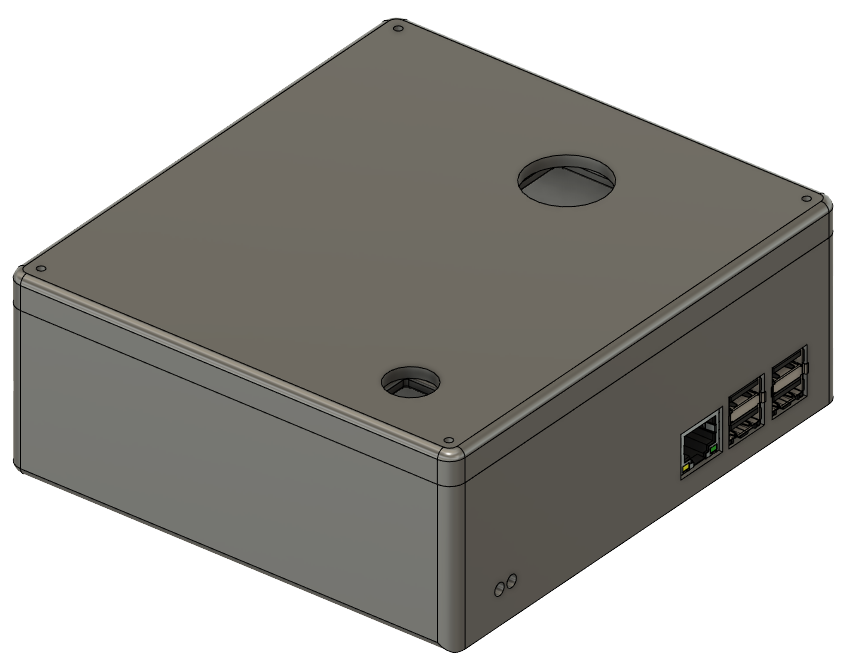
\includegraphics[scale=0.4]{img/el_prototype/box1}
  \caption{Vue des faces avant et supérieure avec le couvercle}
  \label{fig:box1}
\end{figure}


\begin{figure}[ht!]
  \centering
  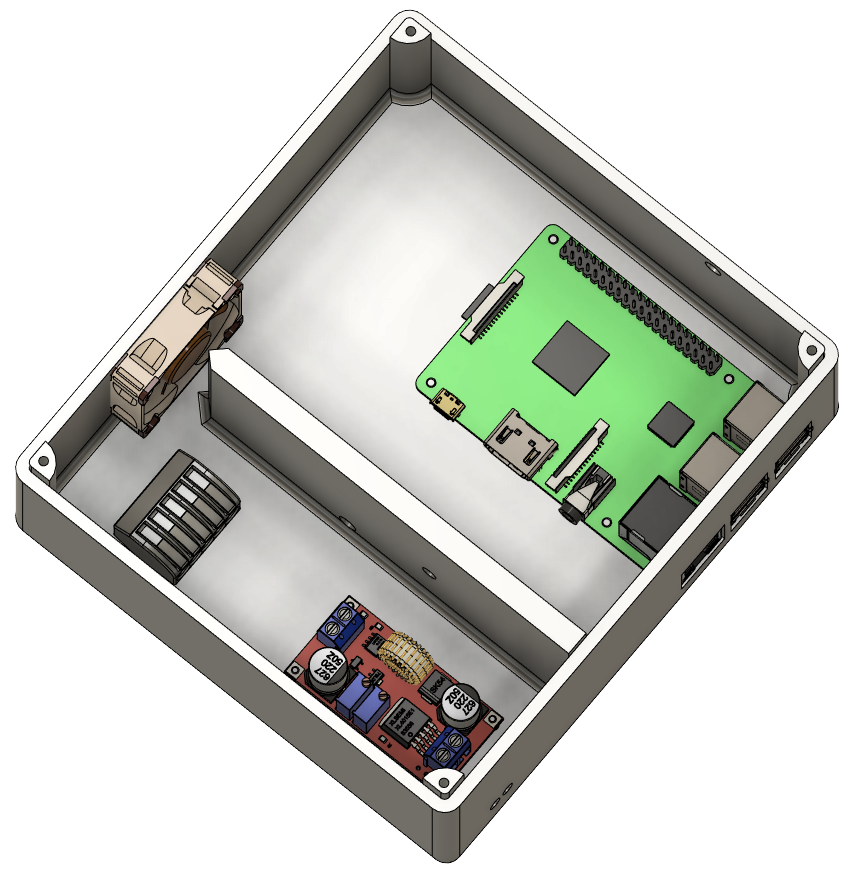
\includegraphics[scale=0.4]{img/el_prototype/box2}
  \caption{Vue de la face supérieure sans le couvercle}
  \label{fig:box2}
\end{figure}

\begin{figure}[ht!]
  \centering
  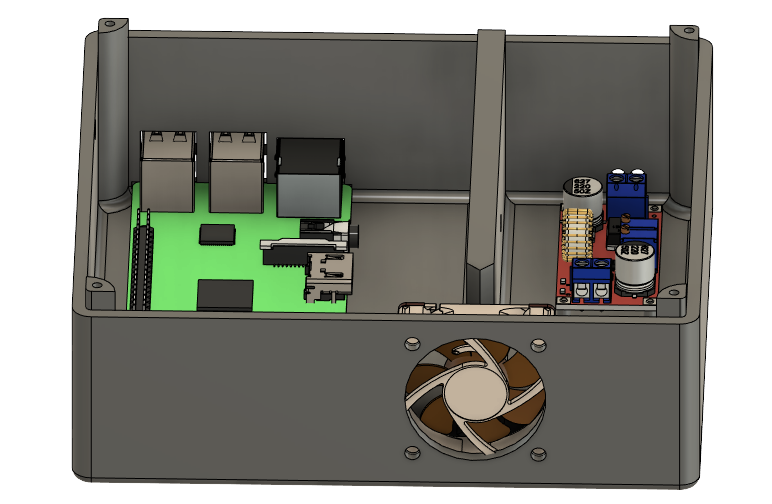
\includegraphics[scale=0.4]{img/el_prototype/box3}
  \caption{Vue de la face arrière sans le couvercle}
  \label{fig:box3}
\end{figure}

~

\noindent
Afin de valider le boîtier, le protocole de test présenté dans la section \ref{sec:prototests} a été à nouveau employé. Dans le premier test (test 5), aucun matériau de blindage magnétique n'a été utilisé. Toutefois, la distance accrue entre le step-down et le SIM800L suffit déjà pour que la communication entre le Raspberry et le modem ait lieu sans aucun problème. Ajouter des feuilles de papier d'aluminium sur la paroi permet de diminuer encore plus l'impact du champ magnétique puisque le nombre d'erreurs est divisé par deux. (voir test 6 sur \ref{tab:res22}). En particulier, cette dernière solution s'est montrée presque aussi efficace qu'éloigner le step-down 50 cm du boîtier.

~

\noindent
La solution de refroidissement de ce boîtier est également très performante puisque la température dans les deux zones (Raspberry Pi et step-down) est tout à fait identique. Ceci montre donc que l'importance du boîtier ne peut pas être négligée. En effet, avoir un boîtier adapté aux besoins des composants est essentiel afin d'assurer le bon fonctionnement de ces derniers et de prolonger leur durée de vie.


\begin{figure}[ht!]
  \centering
  %% Creator: Matplotlib, PGF backend
%%
%% To include the figure in your LaTeX document, write
%%   \input{<filename>.pgf}
%%
%% Make sure the required packages are loaded in your preamble
%%   \usepackage{pgf}
%%
%% Figures using additional raster images can only be included by \input if
%% they are in the same directory as the main LaTeX file. For loading figures
%% from other directories you can use the `import` package
%%   \usepackage{import}
%% and then include the figures with
%%   \import{<path to file>}{<filename>.pgf}
%%
%% Matplotlib used the following preamble
%%
\begingroup%
\makeatletter%
\begin{pgfpicture}%
\pgfpathrectangle{\pgfpointorigin}{\pgfqpoint{5.590556in}{4.068988in}}%
\pgfusepath{use as bounding box, clip}%
\begin{pgfscope}%
\pgfsetbuttcap%
\pgfsetmiterjoin%
\definecolor{currentfill}{rgb}{1.000000,1.000000,1.000000}%
\pgfsetfillcolor{currentfill}%
\pgfsetlinewidth{0.000000pt}%
\definecolor{currentstroke}{rgb}{1.000000,1.000000,1.000000}%
\pgfsetstrokecolor{currentstroke}%
\pgfsetdash{}{0pt}%
\pgfpathmoveto{\pgfqpoint{0.000000in}{0.000000in}}%
\pgfpathlineto{\pgfqpoint{5.590556in}{0.000000in}}%
\pgfpathlineto{\pgfqpoint{5.590556in}{4.068988in}}%
\pgfpathlineto{\pgfqpoint{0.000000in}{4.068988in}}%
\pgfpathclose%
\pgfusepath{fill}%
\end{pgfscope}%
\begin{pgfscope}%
\pgfsetbuttcap%
\pgfsetmiterjoin%
\definecolor{currentfill}{rgb}{1.000000,1.000000,1.000000}%
\pgfsetfillcolor{currentfill}%
\pgfsetlinewidth{0.000000pt}%
\definecolor{currentstroke}{rgb}{0.000000,0.000000,0.000000}%
\pgfsetstrokecolor{currentstroke}%
\pgfsetstrokeopacity{0.000000}%
\pgfsetdash{}{0pt}%
\pgfpathmoveto{\pgfqpoint{0.530556in}{0.656763in}}%
\pgfpathlineto{\pgfqpoint{5.490556in}{0.656763in}}%
\pgfpathlineto{\pgfqpoint{5.490556in}{3.920763in}}%
\pgfpathlineto{\pgfqpoint{0.530556in}{3.920763in}}%
\pgfpathclose%
\pgfusepath{fill}%
\end{pgfscope}%
\begin{pgfscope}%
\pgfsetbuttcap%
\pgfsetroundjoin%
\definecolor{currentfill}{rgb}{0.000000,0.000000,0.000000}%
\pgfsetfillcolor{currentfill}%
\pgfsetlinewidth{0.803000pt}%
\definecolor{currentstroke}{rgb}{0.000000,0.000000,0.000000}%
\pgfsetstrokecolor{currentstroke}%
\pgfsetdash{}{0pt}%
\pgfsys@defobject{currentmarker}{\pgfqpoint{0.000000in}{-0.048611in}}{\pgfqpoint{0.000000in}{0.000000in}}{%
\pgfpathmoveto{\pgfqpoint{0.000000in}{0.000000in}}%
\pgfpathlineto{\pgfqpoint{0.000000in}{-0.048611in}}%
\pgfusepath{stroke,fill}%
}%
\begin{pgfscope}%
\pgfsys@transformshift{0.530556in}{0.656763in}%
\pgfsys@useobject{currentmarker}{}%
\end{pgfscope}%
\end{pgfscope}%
\begin{pgfscope}%
\definecolor{textcolor}{rgb}{0.000000,0.000000,0.000000}%
\pgfsetstrokecolor{textcolor}%
\pgfsetfillcolor{textcolor}%
\pgftext[x=0.243078in,y=0.317832in,left,base,rotate=30.000000]{\color{textcolor}\rmfamily\fontsize{10.000000}{12.000000}\selectfont 00:00}%
\end{pgfscope}%
\begin{pgfscope}%
\pgfsetbuttcap%
\pgfsetroundjoin%
\definecolor{currentfill}{rgb}{0.000000,0.000000,0.000000}%
\pgfsetfillcolor{currentfill}%
\pgfsetlinewidth{0.803000pt}%
\definecolor{currentstroke}{rgb}{0.000000,0.000000,0.000000}%
\pgfsetstrokecolor{currentstroke}%
\pgfsetdash{}{0pt}%
\pgfsys@defobject{currentmarker}{\pgfqpoint{0.000000in}{-0.048611in}}{\pgfqpoint{0.000000in}{0.000000in}}{%
\pgfpathmoveto{\pgfqpoint{0.000000in}{0.000000in}}%
\pgfpathlineto{\pgfqpoint{0.000000in}{-0.048611in}}%
\pgfusepath{stroke,fill}%
}%
\begin{pgfscope}%
\pgfsys@transformshift{1.522519in}{0.656763in}%
\pgfsys@useobject{currentmarker}{}%
\end{pgfscope}%
\end{pgfscope}%
\begin{pgfscope}%
\definecolor{textcolor}{rgb}{0.000000,0.000000,0.000000}%
\pgfsetstrokecolor{textcolor}%
\pgfsetfillcolor{textcolor}%
\pgftext[x=1.235041in,y=0.317832in,left,base,rotate=30.000000]{\color{textcolor}\rmfamily\fontsize{10.000000}{12.000000}\selectfont 01:00}%
\end{pgfscope}%
\begin{pgfscope}%
\pgfsetbuttcap%
\pgfsetroundjoin%
\definecolor{currentfill}{rgb}{0.000000,0.000000,0.000000}%
\pgfsetfillcolor{currentfill}%
\pgfsetlinewidth{0.803000pt}%
\definecolor{currentstroke}{rgb}{0.000000,0.000000,0.000000}%
\pgfsetstrokecolor{currentstroke}%
\pgfsetdash{}{0pt}%
\pgfsys@defobject{currentmarker}{\pgfqpoint{0.000000in}{-0.048611in}}{\pgfqpoint{0.000000in}{0.000000in}}{%
\pgfpathmoveto{\pgfqpoint{0.000000in}{0.000000in}}%
\pgfpathlineto{\pgfqpoint{0.000000in}{-0.048611in}}%
\pgfusepath{stroke,fill}%
}%
\begin{pgfscope}%
\pgfsys@transformshift{2.514481in}{0.656763in}%
\pgfsys@useobject{currentmarker}{}%
\end{pgfscope}%
\end{pgfscope}%
\begin{pgfscope}%
\definecolor{textcolor}{rgb}{0.000000,0.000000,0.000000}%
\pgfsetstrokecolor{textcolor}%
\pgfsetfillcolor{textcolor}%
\pgftext[x=2.227003in,y=0.317832in,left,base,rotate=30.000000]{\color{textcolor}\rmfamily\fontsize{10.000000}{12.000000}\selectfont 02:00}%
\end{pgfscope}%
\begin{pgfscope}%
\pgfsetbuttcap%
\pgfsetroundjoin%
\definecolor{currentfill}{rgb}{0.000000,0.000000,0.000000}%
\pgfsetfillcolor{currentfill}%
\pgfsetlinewidth{0.803000pt}%
\definecolor{currentstroke}{rgb}{0.000000,0.000000,0.000000}%
\pgfsetstrokecolor{currentstroke}%
\pgfsetdash{}{0pt}%
\pgfsys@defobject{currentmarker}{\pgfqpoint{0.000000in}{-0.048611in}}{\pgfqpoint{0.000000in}{0.000000in}}{%
\pgfpathmoveto{\pgfqpoint{0.000000in}{0.000000in}}%
\pgfpathlineto{\pgfqpoint{0.000000in}{-0.048611in}}%
\pgfusepath{stroke,fill}%
}%
\begin{pgfscope}%
\pgfsys@transformshift{3.506444in}{0.656763in}%
\pgfsys@useobject{currentmarker}{}%
\end{pgfscope}%
\end{pgfscope}%
\begin{pgfscope}%
\definecolor{textcolor}{rgb}{0.000000,0.000000,0.000000}%
\pgfsetstrokecolor{textcolor}%
\pgfsetfillcolor{textcolor}%
\pgftext[x=3.218966in,y=0.317832in,left,base,rotate=30.000000]{\color{textcolor}\rmfamily\fontsize{10.000000}{12.000000}\selectfont 03:00}%
\end{pgfscope}%
\begin{pgfscope}%
\pgfsetbuttcap%
\pgfsetroundjoin%
\definecolor{currentfill}{rgb}{0.000000,0.000000,0.000000}%
\pgfsetfillcolor{currentfill}%
\pgfsetlinewidth{0.803000pt}%
\definecolor{currentstroke}{rgb}{0.000000,0.000000,0.000000}%
\pgfsetstrokecolor{currentstroke}%
\pgfsetdash{}{0pt}%
\pgfsys@defobject{currentmarker}{\pgfqpoint{0.000000in}{-0.048611in}}{\pgfqpoint{0.000000in}{0.000000in}}{%
\pgfpathmoveto{\pgfqpoint{0.000000in}{0.000000in}}%
\pgfpathlineto{\pgfqpoint{0.000000in}{-0.048611in}}%
\pgfusepath{stroke,fill}%
}%
\begin{pgfscope}%
\pgfsys@transformshift{4.498407in}{0.656763in}%
\pgfsys@useobject{currentmarker}{}%
\end{pgfscope}%
\end{pgfscope}%
\begin{pgfscope}%
\definecolor{textcolor}{rgb}{0.000000,0.000000,0.000000}%
\pgfsetstrokecolor{textcolor}%
\pgfsetfillcolor{textcolor}%
\pgftext[x=4.210929in,y=0.317832in,left,base,rotate=30.000000]{\color{textcolor}\rmfamily\fontsize{10.000000}{12.000000}\selectfont 04:00}%
\end{pgfscope}%
\begin{pgfscope}%
\pgfsetbuttcap%
\pgfsetroundjoin%
\definecolor{currentfill}{rgb}{0.000000,0.000000,0.000000}%
\pgfsetfillcolor{currentfill}%
\pgfsetlinewidth{0.803000pt}%
\definecolor{currentstroke}{rgb}{0.000000,0.000000,0.000000}%
\pgfsetstrokecolor{currentstroke}%
\pgfsetdash{}{0pt}%
\pgfsys@defobject{currentmarker}{\pgfqpoint{0.000000in}{-0.048611in}}{\pgfqpoint{0.000000in}{0.000000in}}{%
\pgfpathmoveto{\pgfqpoint{0.000000in}{0.000000in}}%
\pgfpathlineto{\pgfqpoint{0.000000in}{-0.048611in}}%
\pgfusepath{stroke,fill}%
}%
\begin{pgfscope}%
\pgfsys@transformshift{5.490369in}{0.656763in}%
\pgfsys@useobject{currentmarker}{}%
\end{pgfscope}%
\end{pgfscope}%
\begin{pgfscope}%
\definecolor{textcolor}{rgb}{0.000000,0.000000,0.000000}%
\pgfsetstrokecolor{textcolor}%
\pgfsetfillcolor{textcolor}%
\pgftext[x=5.202891in,y=0.317832in,left,base,rotate=30.000000]{\color{textcolor}\rmfamily\fontsize{10.000000}{12.000000}\selectfont 05:00}%
\end{pgfscope}%
\begin{pgfscope}%
\definecolor{textcolor}{rgb}{0.000000,0.000000,0.000000}%
\pgfsetstrokecolor{textcolor}%
\pgfsetfillcolor{textcolor}%
\pgftext[x=3.010556in,y=0.238889in,,top]{\color{textcolor}\rmfamily\fontsize{10.000000}{12.000000}\selectfont Temps (hh:mm)}%
\end{pgfscope}%
\begin{pgfscope}%
\pgfsetbuttcap%
\pgfsetroundjoin%
\definecolor{currentfill}{rgb}{0.000000,0.000000,0.000000}%
\pgfsetfillcolor{currentfill}%
\pgfsetlinewidth{0.803000pt}%
\definecolor{currentstroke}{rgb}{0.000000,0.000000,0.000000}%
\pgfsetstrokecolor{currentstroke}%
\pgfsetdash{}{0pt}%
\pgfsys@defobject{currentmarker}{\pgfqpoint{-0.048611in}{0.000000in}}{\pgfqpoint{0.000000in}{0.000000in}}{%
\pgfpathmoveto{\pgfqpoint{0.000000in}{0.000000in}}%
\pgfpathlineto{\pgfqpoint{-0.048611in}{0.000000in}}%
\pgfusepath{stroke,fill}%
}%
\begin{pgfscope}%
\pgfsys@transformshift{0.530556in}{0.656763in}%
\pgfsys@useobject{currentmarker}{}%
\end{pgfscope}%
\end{pgfscope}%
\begin{pgfscope}%
\definecolor{textcolor}{rgb}{0.000000,0.000000,0.000000}%
\pgfsetstrokecolor{textcolor}%
\pgfsetfillcolor{textcolor}%
\pgftext[x=0.294444in,y=0.608538in,left,base]{\color{textcolor}\rmfamily\fontsize{10.000000}{12.000000}\selectfont \(\displaystyle 20\)}%
\end{pgfscope}%
\begin{pgfscope}%
\pgfsetbuttcap%
\pgfsetroundjoin%
\definecolor{currentfill}{rgb}{0.000000,0.000000,0.000000}%
\pgfsetfillcolor{currentfill}%
\pgfsetlinewidth{0.803000pt}%
\definecolor{currentstroke}{rgb}{0.000000,0.000000,0.000000}%
\pgfsetstrokecolor{currentstroke}%
\pgfsetdash{}{0pt}%
\pgfsys@defobject{currentmarker}{\pgfqpoint{-0.048611in}{0.000000in}}{\pgfqpoint{0.000000in}{0.000000in}}{%
\pgfpathmoveto{\pgfqpoint{0.000000in}{0.000000in}}%
\pgfpathlineto{\pgfqpoint{-0.048611in}{0.000000in}}%
\pgfusepath{stroke,fill}%
}%
\begin{pgfscope}%
\pgfsys@transformshift{0.530556in}{1.123049in}%
\pgfsys@useobject{currentmarker}{}%
\end{pgfscope}%
\end{pgfscope}%
\begin{pgfscope}%
\definecolor{textcolor}{rgb}{0.000000,0.000000,0.000000}%
\pgfsetstrokecolor{textcolor}%
\pgfsetfillcolor{textcolor}%
\pgftext[x=0.294444in,y=1.074823in,left,base]{\color{textcolor}\rmfamily\fontsize{10.000000}{12.000000}\selectfont \(\displaystyle 25\)}%
\end{pgfscope}%
\begin{pgfscope}%
\pgfsetbuttcap%
\pgfsetroundjoin%
\definecolor{currentfill}{rgb}{0.000000,0.000000,0.000000}%
\pgfsetfillcolor{currentfill}%
\pgfsetlinewidth{0.803000pt}%
\definecolor{currentstroke}{rgb}{0.000000,0.000000,0.000000}%
\pgfsetstrokecolor{currentstroke}%
\pgfsetdash{}{0pt}%
\pgfsys@defobject{currentmarker}{\pgfqpoint{-0.048611in}{0.000000in}}{\pgfqpoint{0.000000in}{0.000000in}}{%
\pgfpathmoveto{\pgfqpoint{0.000000in}{0.000000in}}%
\pgfpathlineto{\pgfqpoint{-0.048611in}{0.000000in}}%
\pgfusepath{stroke,fill}%
}%
\begin{pgfscope}%
\pgfsys@transformshift{0.530556in}{1.589334in}%
\pgfsys@useobject{currentmarker}{}%
\end{pgfscope}%
\end{pgfscope}%
\begin{pgfscope}%
\definecolor{textcolor}{rgb}{0.000000,0.000000,0.000000}%
\pgfsetstrokecolor{textcolor}%
\pgfsetfillcolor{textcolor}%
\pgftext[x=0.294444in,y=1.541109in,left,base]{\color{textcolor}\rmfamily\fontsize{10.000000}{12.000000}\selectfont \(\displaystyle 30\)}%
\end{pgfscope}%
\begin{pgfscope}%
\pgfsetbuttcap%
\pgfsetroundjoin%
\definecolor{currentfill}{rgb}{0.000000,0.000000,0.000000}%
\pgfsetfillcolor{currentfill}%
\pgfsetlinewidth{0.803000pt}%
\definecolor{currentstroke}{rgb}{0.000000,0.000000,0.000000}%
\pgfsetstrokecolor{currentstroke}%
\pgfsetdash{}{0pt}%
\pgfsys@defobject{currentmarker}{\pgfqpoint{-0.048611in}{0.000000in}}{\pgfqpoint{0.000000in}{0.000000in}}{%
\pgfpathmoveto{\pgfqpoint{0.000000in}{0.000000in}}%
\pgfpathlineto{\pgfqpoint{-0.048611in}{0.000000in}}%
\pgfusepath{stroke,fill}%
}%
\begin{pgfscope}%
\pgfsys@transformshift{0.530556in}{2.055620in}%
\pgfsys@useobject{currentmarker}{}%
\end{pgfscope}%
\end{pgfscope}%
\begin{pgfscope}%
\definecolor{textcolor}{rgb}{0.000000,0.000000,0.000000}%
\pgfsetstrokecolor{textcolor}%
\pgfsetfillcolor{textcolor}%
\pgftext[x=0.294444in,y=2.007395in,left,base]{\color{textcolor}\rmfamily\fontsize{10.000000}{12.000000}\selectfont \(\displaystyle 35\)}%
\end{pgfscope}%
\begin{pgfscope}%
\pgfsetbuttcap%
\pgfsetroundjoin%
\definecolor{currentfill}{rgb}{0.000000,0.000000,0.000000}%
\pgfsetfillcolor{currentfill}%
\pgfsetlinewidth{0.803000pt}%
\definecolor{currentstroke}{rgb}{0.000000,0.000000,0.000000}%
\pgfsetstrokecolor{currentstroke}%
\pgfsetdash{}{0pt}%
\pgfsys@defobject{currentmarker}{\pgfqpoint{-0.048611in}{0.000000in}}{\pgfqpoint{0.000000in}{0.000000in}}{%
\pgfpathmoveto{\pgfqpoint{0.000000in}{0.000000in}}%
\pgfpathlineto{\pgfqpoint{-0.048611in}{0.000000in}}%
\pgfusepath{stroke,fill}%
}%
\begin{pgfscope}%
\pgfsys@transformshift{0.530556in}{2.521906in}%
\pgfsys@useobject{currentmarker}{}%
\end{pgfscope}%
\end{pgfscope}%
\begin{pgfscope}%
\definecolor{textcolor}{rgb}{0.000000,0.000000,0.000000}%
\pgfsetstrokecolor{textcolor}%
\pgfsetfillcolor{textcolor}%
\pgftext[x=0.294444in,y=2.473680in,left,base]{\color{textcolor}\rmfamily\fontsize{10.000000}{12.000000}\selectfont \(\displaystyle 40\)}%
\end{pgfscope}%
\begin{pgfscope}%
\pgfsetbuttcap%
\pgfsetroundjoin%
\definecolor{currentfill}{rgb}{0.000000,0.000000,0.000000}%
\pgfsetfillcolor{currentfill}%
\pgfsetlinewidth{0.803000pt}%
\definecolor{currentstroke}{rgb}{0.000000,0.000000,0.000000}%
\pgfsetstrokecolor{currentstroke}%
\pgfsetdash{}{0pt}%
\pgfsys@defobject{currentmarker}{\pgfqpoint{-0.048611in}{0.000000in}}{\pgfqpoint{0.000000in}{0.000000in}}{%
\pgfpathmoveto{\pgfqpoint{0.000000in}{0.000000in}}%
\pgfpathlineto{\pgfqpoint{-0.048611in}{0.000000in}}%
\pgfusepath{stroke,fill}%
}%
\begin{pgfscope}%
\pgfsys@transformshift{0.530556in}{2.988191in}%
\pgfsys@useobject{currentmarker}{}%
\end{pgfscope}%
\end{pgfscope}%
\begin{pgfscope}%
\definecolor{textcolor}{rgb}{0.000000,0.000000,0.000000}%
\pgfsetstrokecolor{textcolor}%
\pgfsetfillcolor{textcolor}%
\pgftext[x=0.294444in,y=2.939966in,left,base]{\color{textcolor}\rmfamily\fontsize{10.000000}{12.000000}\selectfont \(\displaystyle 45\)}%
\end{pgfscope}%
\begin{pgfscope}%
\pgfsetbuttcap%
\pgfsetroundjoin%
\definecolor{currentfill}{rgb}{0.000000,0.000000,0.000000}%
\pgfsetfillcolor{currentfill}%
\pgfsetlinewidth{0.803000pt}%
\definecolor{currentstroke}{rgb}{0.000000,0.000000,0.000000}%
\pgfsetstrokecolor{currentstroke}%
\pgfsetdash{}{0pt}%
\pgfsys@defobject{currentmarker}{\pgfqpoint{-0.048611in}{0.000000in}}{\pgfqpoint{0.000000in}{0.000000in}}{%
\pgfpathmoveto{\pgfqpoint{0.000000in}{0.000000in}}%
\pgfpathlineto{\pgfqpoint{-0.048611in}{0.000000in}}%
\pgfusepath{stroke,fill}%
}%
\begin{pgfscope}%
\pgfsys@transformshift{0.530556in}{3.454477in}%
\pgfsys@useobject{currentmarker}{}%
\end{pgfscope}%
\end{pgfscope}%
\begin{pgfscope}%
\definecolor{textcolor}{rgb}{0.000000,0.000000,0.000000}%
\pgfsetstrokecolor{textcolor}%
\pgfsetfillcolor{textcolor}%
\pgftext[x=0.294444in,y=3.406252in,left,base]{\color{textcolor}\rmfamily\fontsize{10.000000}{12.000000}\selectfont \(\displaystyle 50\)}%
\end{pgfscope}%
\begin{pgfscope}%
\pgfsetbuttcap%
\pgfsetroundjoin%
\definecolor{currentfill}{rgb}{0.000000,0.000000,0.000000}%
\pgfsetfillcolor{currentfill}%
\pgfsetlinewidth{0.803000pt}%
\definecolor{currentstroke}{rgb}{0.000000,0.000000,0.000000}%
\pgfsetstrokecolor{currentstroke}%
\pgfsetdash{}{0pt}%
\pgfsys@defobject{currentmarker}{\pgfqpoint{-0.048611in}{0.000000in}}{\pgfqpoint{0.000000in}{0.000000in}}{%
\pgfpathmoveto{\pgfqpoint{0.000000in}{0.000000in}}%
\pgfpathlineto{\pgfqpoint{-0.048611in}{0.000000in}}%
\pgfusepath{stroke,fill}%
}%
\begin{pgfscope}%
\pgfsys@transformshift{0.530556in}{3.920763in}%
\pgfsys@useobject{currentmarker}{}%
\end{pgfscope}%
\end{pgfscope}%
\begin{pgfscope}%
\definecolor{textcolor}{rgb}{0.000000,0.000000,0.000000}%
\pgfsetstrokecolor{textcolor}%
\pgfsetfillcolor{textcolor}%
\pgftext[x=0.294444in,y=3.872538in,left,base]{\color{textcolor}\rmfamily\fontsize{10.000000}{12.000000}\selectfont \(\displaystyle 55\)}%
\end{pgfscope}%
\begin{pgfscope}%
\definecolor{textcolor}{rgb}{0.000000,0.000000,0.000000}%
\pgfsetstrokecolor{textcolor}%
\pgfsetfillcolor{textcolor}%
\pgftext[x=0.238889in,y=2.288763in,,bottom,rotate=90.000000]{\color{textcolor}\rmfamily\fontsize{10.000000}{12.000000}\selectfont Température (\textdegree{}C)}%
\end{pgfscope}%
\begin{pgfscope}%
\pgfpathrectangle{\pgfqpoint{0.530556in}{0.656763in}}{\pgfqpoint{4.960000in}{3.264000in}}%
\pgfusepath{clip}%
\pgfsetrectcap%
\pgfsetroundjoin%
\pgfsetlinewidth{1.505625pt}%
\definecolor{currentstroke}{rgb}{0.121569,0.466667,0.705882}%
\pgfsetstrokecolor{currentstroke}%
\pgfsetdash{}{0pt}%
\pgfpathmoveto{\pgfqpoint{0.538832in}{1.912626in}}%
\pgfpathlineto{\pgfqpoint{0.547107in}{1.946820in}}%
\pgfpathlineto{\pgfqpoint{0.555385in}{1.993449in}}%
\pgfpathlineto{\pgfqpoint{0.563663in}{1.993449in}}%
\pgfpathlineto{\pgfqpoint{0.571939in}{1.977906in}}%
\pgfpathlineto{\pgfqpoint{0.580217in}{1.977906in}}%
\pgfpathlineto{\pgfqpoint{0.596772in}{2.008991in}}%
\pgfpathlineto{\pgfqpoint{0.605042in}{2.012100in}}%
\pgfpathlineto{\pgfqpoint{0.613318in}{2.008991in}}%
\pgfpathlineto{\pgfqpoint{0.621592in}{2.043186in}}%
\pgfpathlineto{\pgfqpoint{0.629865in}{2.043186in}}%
\pgfpathlineto{\pgfqpoint{0.638139in}{2.061837in}}%
\pgfpathlineto{\pgfqpoint{0.646412in}{2.061837in}}%
\pgfpathlineto{\pgfqpoint{0.654687in}{2.027643in}}%
\pgfpathlineto{\pgfqpoint{0.662960in}{2.080489in}}%
\pgfpathlineto{\pgfqpoint{0.671232in}{2.043186in}}%
\pgfpathlineto{\pgfqpoint{0.679507in}{2.046294in}}%
\pgfpathlineto{\pgfqpoint{0.687780in}{2.027643in}}%
\pgfpathlineto{\pgfqpoint{0.696053in}{2.046294in}}%
\pgfpathlineto{\pgfqpoint{0.704327in}{2.061837in}}%
\pgfpathlineto{\pgfqpoint{0.712605in}{2.043186in}}%
\pgfpathlineto{\pgfqpoint{0.720880in}{2.046294in}}%
\pgfpathlineto{\pgfqpoint{0.729153in}{2.043186in}}%
\pgfpathlineto{\pgfqpoint{0.737425in}{2.080489in}}%
\pgfpathlineto{\pgfqpoint{0.753979in}{2.043186in}}%
\pgfpathlineto{\pgfqpoint{0.762255in}{2.080489in}}%
\pgfpathlineto{\pgfqpoint{0.770532in}{2.027643in}}%
\pgfpathlineto{\pgfqpoint{0.778805in}{2.061837in}}%
\pgfpathlineto{\pgfqpoint{0.787077in}{2.027643in}}%
\pgfpathlineto{\pgfqpoint{0.795351in}{2.061837in}}%
\pgfpathlineto{\pgfqpoint{0.803624in}{2.046294in}}%
\pgfpathlineto{\pgfqpoint{0.811897in}{2.027643in}}%
\pgfpathlineto{\pgfqpoint{0.820168in}{2.043186in}}%
\pgfpathlineto{\pgfqpoint{0.828443in}{2.043186in}}%
\pgfpathlineto{\pgfqpoint{0.836716in}{2.061837in}}%
\pgfpathlineto{\pgfqpoint{0.844990in}{2.043186in}}%
\pgfpathlineto{\pgfqpoint{0.853261in}{2.061837in}}%
\pgfpathlineto{\pgfqpoint{0.861536in}{2.043186in}}%
\pgfpathlineto{\pgfqpoint{0.869814in}{2.080489in}}%
\pgfpathlineto{\pgfqpoint{0.878087in}{2.061837in}}%
\pgfpathlineto{\pgfqpoint{0.894640in}{2.061837in}}%
\pgfpathlineto{\pgfqpoint{0.902918in}{2.027643in}}%
\pgfpathlineto{\pgfqpoint{0.911190in}{2.027643in}}%
\pgfpathlineto{\pgfqpoint{0.919466in}{2.061837in}}%
\pgfpathlineto{\pgfqpoint{0.927741in}{2.080489in}}%
\pgfpathlineto{\pgfqpoint{0.936017in}{2.061837in}}%
\pgfpathlineto{\pgfqpoint{0.944294in}{2.061837in}}%
\pgfpathlineto{\pgfqpoint{0.952572in}{2.096031in}}%
\pgfpathlineto{\pgfqpoint{0.960850in}{2.043186in}}%
\pgfpathlineto{\pgfqpoint{0.969127in}{2.043186in}}%
\pgfpathlineto{\pgfqpoint{0.985678in}{2.080489in}}%
\pgfpathlineto{\pgfqpoint{0.993958in}{2.080489in}}%
\pgfpathlineto{\pgfqpoint{1.002237in}{2.061837in}}%
\pgfpathlineto{\pgfqpoint{1.010514in}{2.061837in}}%
\pgfpathlineto{\pgfqpoint{1.018793in}{2.043186in}}%
\pgfpathlineto{\pgfqpoint{1.027071in}{2.080489in}}%
\pgfpathlineto{\pgfqpoint{1.035349in}{2.061837in}}%
\pgfpathlineto{\pgfqpoint{1.043627in}{2.080489in}}%
\pgfpathlineto{\pgfqpoint{1.051905in}{2.061837in}}%
\pgfpathlineto{\pgfqpoint{1.068461in}{2.061837in}}%
\pgfpathlineto{\pgfqpoint{1.076734in}{2.080489in}}%
\pgfpathlineto{\pgfqpoint{1.093279in}{2.080489in}}%
\pgfpathlineto{\pgfqpoint{1.101552in}{2.077380in}}%
\pgfpathlineto{\pgfqpoint{1.109830in}{2.080489in}}%
\pgfpathlineto{\pgfqpoint{1.176039in}{2.080489in}}%
\pgfpathlineto{\pgfqpoint{1.184316in}{2.046294in}}%
\pgfpathlineto{\pgfqpoint{1.192594in}{2.080489in}}%
\pgfpathlineto{\pgfqpoint{1.200871in}{2.096031in}}%
\pgfpathlineto{\pgfqpoint{1.209148in}{2.043186in}}%
\pgfpathlineto{\pgfqpoint{1.217426in}{2.008991in}}%
\pgfpathlineto{\pgfqpoint{1.225703in}{2.043186in}}%
\pgfpathlineto{\pgfqpoint{1.242258in}{2.080489in}}%
\pgfpathlineto{\pgfqpoint{1.250535in}{2.043186in}}%
\pgfpathlineto{\pgfqpoint{1.258813in}{2.080489in}}%
\pgfpathlineto{\pgfqpoint{1.267091in}{2.061837in}}%
\pgfpathlineto{\pgfqpoint{1.275367in}{2.077380in}}%
\pgfpathlineto{\pgfqpoint{1.283642in}{2.061837in}}%
\pgfpathlineto{\pgfqpoint{1.291917in}{2.061837in}}%
\pgfpathlineto{\pgfqpoint{1.308466in}{2.024534in}}%
\pgfpathlineto{\pgfqpoint{1.316741in}{2.046294in}}%
\pgfpathlineto{\pgfqpoint{1.325015in}{2.027643in}}%
\pgfpathlineto{\pgfqpoint{1.333290in}{2.043186in}}%
\pgfpathlineto{\pgfqpoint{1.341567in}{2.080489in}}%
\pgfpathlineto{\pgfqpoint{1.349845in}{2.024534in}}%
\pgfpathlineto{\pgfqpoint{1.358122in}{2.061837in}}%
\pgfpathlineto{\pgfqpoint{1.366399in}{1.993449in}}%
\pgfpathlineto{\pgfqpoint{1.374677in}{2.027643in}}%
\pgfpathlineto{\pgfqpoint{1.382954in}{2.012100in}}%
\pgfpathlineto{\pgfqpoint{1.391232in}{2.027643in}}%
\pgfpathlineto{\pgfqpoint{1.399510in}{2.046294in}}%
\pgfpathlineto{\pgfqpoint{1.407787in}{2.027643in}}%
\pgfpathlineto{\pgfqpoint{1.424344in}{2.027643in}}%
\pgfpathlineto{\pgfqpoint{1.432621in}{2.046294in}}%
\pgfpathlineto{\pgfqpoint{1.440897in}{2.046294in}}%
\pgfpathlineto{\pgfqpoint{1.449175in}{2.061837in}}%
\pgfpathlineto{\pgfqpoint{1.457452in}{2.046294in}}%
\pgfpathlineto{\pgfqpoint{1.465725in}{2.024534in}}%
\pgfpathlineto{\pgfqpoint{1.473999in}{2.027643in}}%
\pgfpathlineto{\pgfqpoint{1.482277in}{2.027643in}}%
\pgfpathlineto{\pgfqpoint{1.490551in}{2.043186in}}%
\pgfpathlineto{\pgfqpoint{1.498829in}{2.027643in}}%
\pgfpathlineto{\pgfqpoint{1.515383in}{2.027643in}}%
\pgfpathlineto{\pgfqpoint{1.523657in}{2.046294in}}%
\pgfpathlineto{\pgfqpoint{1.531935in}{2.061837in}}%
\pgfpathlineto{\pgfqpoint{1.540212in}{2.046294in}}%
\pgfpathlineto{\pgfqpoint{1.548489in}{2.043186in}}%
\pgfpathlineto{\pgfqpoint{1.556764in}{2.027643in}}%
\pgfpathlineto{\pgfqpoint{1.565040in}{2.027643in}}%
\pgfpathlineto{\pgfqpoint{1.573312in}{2.043186in}}%
\pgfpathlineto{\pgfqpoint{1.581586in}{2.027643in}}%
\pgfpathlineto{\pgfqpoint{1.589859in}{2.046294in}}%
\pgfpathlineto{\pgfqpoint{1.598137in}{2.024534in}}%
\pgfpathlineto{\pgfqpoint{1.606414in}{2.027643in}}%
\pgfpathlineto{\pgfqpoint{1.614691in}{2.046294in}}%
\pgfpathlineto{\pgfqpoint{1.622963in}{2.043186in}}%
\pgfpathlineto{\pgfqpoint{1.631240in}{2.027643in}}%
\pgfpathlineto{\pgfqpoint{1.639511in}{2.046294in}}%
\pgfpathlineto{\pgfqpoint{1.647788in}{2.027643in}}%
\pgfpathlineto{\pgfqpoint{1.656066in}{2.061837in}}%
\pgfpathlineto{\pgfqpoint{1.664344in}{2.043186in}}%
\pgfpathlineto{\pgfqpoint{1.672621in}{2.061837in}}%
\pgfpathlineto{\pgfqpoint{1.680899in}{2.027643in}}%
\pgfpathlineto{\pgfqpoint{1.689176in}{2.046294in}}%
\pgfpathlineto{\pgfqpoint{1.705726in}{2.046294in}}%
\pgfpathlineto{\pgfqpoint{1.714001in}{2.080489in}}%
\pgfpathlineto{\pgfqpoint{1.722277in}{2.043186in}}%
\pgfpathlineto{\pgfqpoint{1.730549in}{2.080489in}}%
\pgfpathlineto{\pgfqpoint{1.738826in}{2.080489in}}%
\pgfpathlineto{\pgfqpoint{1.747103in}{2.077380in}}%
\pgfpathlineto{\pgfqpoint{1.755375in}{2.061837in}}%
\pgfpathlineto{\pgfqpoint{1.763651in}{2.043186in}}%
\pgfpathlineto{\pgfqpoint{1.771925in}{2.077380in}}%
\pgfpathlineto{\pgfqpoint{1.780199in}{2.046294in}}%
\pgfpathlineto{\pgfqpoint{1.788477in}{2.061837in}}%
\pgfpathlineto{\pgfqpoint{1.796754in}{2.080489in}}%
\pgfpathlineto{\pgfqpoint{1.805031in}{2.061837in}}%
\pgfpathlineto{\pgfqpoint{1.813309in}{2.096031in}}%
\pgfpathlineto{\pgfqpoint{1.821586in}{2.027643in}}%
\pgfpathlineto{\pgfqpoint{1.829858in}{2.096031in}}%
\pgfpathlineto{\pgfqpoint{1.838130in}{2.046294in}}%
\pgfpathlineto{\pgfqpoint{1.846402in}{2.027643in}}%
\pgfpathlineto{\pgfqpoint{1.854679in}{2.061837in}}%
\pgfpathlineto{\pgfqpoint{1.862957in}{2.046294in}}%
\pgfpathlineto{\pgfqpoint{1.871232in}{2.061837in}}%
\pgfpathlineto{\pgfqpoint{1.896050in}{2.061837in}}%
\pgfpathlineto{\pgfqpoint{1.904328in}{2.030751in}}%
\pgfpathlineto{\pgfqpoint{1.912606in}{2.061837in}}%
\pgfpathlineto{\pgfqpoint{1.920884in}{2.027643in}}%
\pgfpathlineto{\pgfqpoint{1.929162in}{2.061837in}}%
\pgfpathlineto{\pgfqpoint{1.962273in}{2.061837in}}%
\pgfpathlineto{\pgfqpoint{1.970549in}{2.027643in}}%
\pgfpathlineto{\pgfqpoint{1.978827in}{2.027643in}}%
\pgfpathlineto{\pgfqpoint{1.987105in}{2.043186in}}%
\pgfpathlineto{\pgfqpoint{1.995382in}{2.046294in}}%
\pgfpathlineto{\pgfqpoint{2.003657in}{2.080489in}}%
\pgfpathlineto{\pgfqpoint{2.011930in}{2.027643in}}%
\pgfpathlineto{\pgfqpoint{2.020207in}{2.008991in}}%
\pgfpathlineto{\pgfqpoint{2.028485in}{2.061837in}}%
\pgfpathlineto{\pgfqpoint{2.036763in}{2.024534in}}%
\pgfpathlineto{\pgfqpoint{2.045039in}{2.027643in}}%
\pgfpathlineto{\pgfqpoint{2.053317in}{2.043186in}}%
\pgfpathlineto{\pgfqpoint{2.061595in}{2.080489in}}%
\pgfpathlineto{\pgfqpoint{2.069873in}{2.080489in}}%
\pgfpathlineto{\pgfqpoint{2.078150in}{2.043186in}}%
\pgfpathlineto{\pgfqpoint{2.086428in}{2.061837in}}%
\pgfpathlineto{\pgfqpoint{2.094706in}{2.027643in}}%
\pgfpathlineto{\pgfqpoint{2.102984in}{2.061837in}}%
\pgfpathlineto{\pgfqpoint{2.111262in}{2.080489in}}%
\pgfpathlineto{\pgfqpoint{2.127814in}{2.043186in}}%
\pgfpathlineto{\pgfqpoint{2.136091in}{2.096031in}}%
\pgfpathlineto{\pgfqpoint{2.144363in}{2.061837in}}%
\pgfpathlineto{\pgfqpoint{2.152641in}{2.080489in}}%
\pgfpathlineto{\pgfqpoint{2.160918in}{2.061837in}}%
\pgfpathlineto{\pgfqpoint{2.169195in}{2.080489in}}%
\pgfpathlineto{\pgfqpoint{2.177472in}{2.061837in}}%
\pgfpathlineto{\pgfqpoint{2.185749in}{2.080489in}}%
\pgfpathlineto{\pgfqpoint{2.194019in}{2.043186in}}%
\pgfpathlineto{\pgfqpoint{2.202297in}{2.061837in}}%
\pgfpathlineto{\pgfqpoint{2.210570in}{2.061837in}}%
\pgfpathlineto{\pgfqpoint{2.218848in}{2.080489in}}%
\pgfpathlineto{\pgfqpoint{2.227125in}{2.080489in}}%
\pgfpathlineto{\pgfqpoint{2.235403in}{2.061837in}}%
\pgfpathlineto{\pgfqpoint{2.243676in}{2.080489in}}%
\pgfpathlineto{\pgfqpoint{2.251948in}{2.061837in}}%
\pgfpathlineto{\pgfqpoint{2.276776in}{2.061837in}}%
\pgfpathlineto{\pgfqpoint{2.285050in}{2.080489in}}%
\pgfpathlineto{\pgfqpoint{2.293326in}{2.061837in}}%
\pgfpathlineto{\pgfqpoint{2.301603in}{2.080489in}}%
\pgfpathlineto{\pgfqpoint{2.309880in}{2.061837in}}%
\pgfpathlineto{\pgfqpoint{2.318158in}{2.080489in}}%
\pgfpathlineto{\pgfqpoint{2.326435in}{2.046294in}}%
\pgfpathlineto{\pgfqpoint{2.334712in}{2.061837in}}%
\pgfpathlineto{\pgfqpoint{2.342989in}{2.061837in}}%
\pgfpathlineto{\pgfqpoint{2.351266in}{2.080489in}}%
\pgfpathlineto{\pgfqpoint{2.359544in}{2.043186in}}%
\pgfpathlineto{\pgfqpoint{2.376092in}{2.080489in}}%
\pgfpathlineto{\pgfqpoint{2.384369in}{2.080489in}}%
\pgfpathlineto{\pgfqpoint{2.392641in}{2.096031in}}%
\pgfpathlineto{\pgfqpoint{2.400918in}{2.080489in}}%
\pgfpathlineto{\pgfqpoint{2.409192in}{2.061837in}}%
\pgfpathlineto{\pgfqpoint{2.417467in}{2.080489in}}%
\pgfpathlineto{\pgfqpoint{2.425740in}{2.080489in}}%
\pgfpathlineto{\pgfqpoint{2.434015in}{2.096031in}}%
\pgfpathlineto{\pgfqpoint{2.442290in}{2.080489in}}%
\pgfpathlineto{\pgfqpoint{2.450567in}{2.046294in}}%
\pgfpathlineto{\pgfqpoint{2.458843in}{2.080489in}}%
\pgfpathlineto{\pgfqpoint{2.467121in}{2.061837in}}%
\pgfpathlineto{\pgfqpoint{2.475392in}{2.061837in}}%
\pgfpathlineto{\pgfqpoint{2.483666in}{2.043186in}}%
\pgfpathlineto{\pgfqpoint{2.491938in}{2.080489in}}%
\pgfpathlineto{\pgfqpoint{2.500209in}{2.080489in}}%
\pgfpathlineto{\pgfqpoint{2.508488in}{2.061837in}}%
\pgfpathlineto{\pgfqpoint{2.525040in}{2.061837in}}%
\pgfpathlineto{\pgfqpoint{2.533319in}{2.080489in}}%
\pgfpathlineto{\pgfqpoint{2.566412in}{2.080489in}}%
\pgfpathlineto{\pgfqpoint{2.574689in}{2.061837in}}%
\pgfpathlineto{\pgfqpoint{2.582966in}{2.096031in}}%
\pgfpathlineto{\pgfqpoint{2.591242in}{2.080489in}}%
\pgfpathlineto{\pgfqpoint{2.599519in}{2.077380in}}%
\pgfpathlineto{\pgfqpoint{2.607797in}{2.096031in}}%
\pgfpathlineto{\pgfqpoint{2.616077in}{2.080489in}}%
\pgfpathlineto{\pgfqpoint{2.624351in}{2.061837in}}%
\pgfpathlineto{\pgfqpoint{2.632629in}{2.080489in}}%
\pgfpathlineto{\pgfqpoint{2.640903in}{2.080489in}}%
\pgfpathlineto{\pgfqpoint{2.649175in}{2.027643in}}%
\pgfpathlineto{\pgfqpoint{2.657453in}{2.080489in}}%
\pgfpathlineto{\pgfqpoint{2.665724in}{2.061837in}}%
\pgfpathlineto{\pgfqpoint{2.674002in}{2.080489in}}%
\pgfpathlineto{\pgfqpoint{2.682279in}{2.061837in}}%
\pgfpathlineto{\pgfqpoint{2.690557in}{2.061837in}}%
\pgfpathlineto{\pgfqpoint{2.698835in}{2.077380in}}%
\pgfpathlineto{\pgfqpoint{2.707113in}{2.080489in}}%
\pgfpathlineto{\pgfqpoint{2.715391in}{2.080489in}}%
\pgfpathlineto{\pgfqpoint{2.723669in}{2.043186in}}%
\pgfpathlineto{\pgfqpoint{2.731947in}{2.096031in}}%
\pgfpathlineto{\pgfqpoint{2.740227in}{2.080489in}}%
\pgfpathlineto{\pgfqpoint{2.748498in}{2.096031in}}%
\pgfpathlineto{\pgfqpoint{2.756776in}{2.080489in}}%
\pgfpathlineto{\pgfqpoint{2.773333in}{2.080489in}}%
\pgfpathlineto{\pgfqpoint{2.789889in}{2.043186in}}%
\pgfpathlineto{\pgfqpoint{2.798167in}{2.043186in}}%
\pgfpathlineto{\pgfqpoint{2.806438in}{2.080489in}}%
\pgfpathlineto{\pgfqpoint{2.822992in}{2.080489in}}%
\pgfpathlineto{\pgfqpoint{2.831264in}{2.077380in}}%
\pgfpathlineto{\pgfqpoint{2.839542in}{2.080489in}}%
\pgfpathlineto{\pgfqpoint{2.847820in}{2.096031in}}%
\pgfpathlineto{\pgfqpoint{2.856091in}{2.080489in}}%
\pgfpathlineto{\pgfqpoint{2.864369in}{2.096031in}}%
\pgfpathlineto{\pgfqpoint{2.872647in}{2.061837in}}%
\pgfpathlineto{\pgfqpoint{2.880922in}{2.080489in}}%
\pgfpathlineto{\pgfqpoint{2.897477in}{2.080489in}}%
\pgfpathlineto{\pgfqpoint{2.905755in}{2.096031in}}%
\pgfpathlineto{\pgfqpoint{2.922308in}{2.096031in}}%
\pgfpathlineto{\pgfqpoint{2.930583in}{2.111574in}}%
\pgfpathlineto{\pgfqpoint{2.938860in}{2.080489in}}%
\pgfpathlineto{\pgfqpoint{2.947136in}{2.077380in}}%
\pgfpathlineto{\pgfqpoint{2.955407in}{2.111574in}}%
\pgfpathlineto{\pgfqpoint{2.963680in}{2.080489in}}%
\pgfpathlineto{\pgfqpoint{2.980227in}{2.080489in}}%
\pgfpathlineto{\pgfqpoint{2.988503in}{2.096031in}}%
\pgfpathlineto{\pgfqpoint{3.005056in}{2.096031in}}%
\pgfpathlineto{\pgfqpoint{3.013333in}{2.043186in}}%
\pgfpathlineto{\pgfqpoint{3.021611in}{2.096031in}}%
\pgfpathlineto{\pgfqpoint{3.029888in}{2.080489in}}%
\pgfpathlineto{\pgfqpoint{3.038163in}{2.092923in}}%
\pgfpathlineto{\pgfqpoint{3.046436in}{2.096031in}}%
\pgfpathlineto{\pgfqpoint{3.054714in}{2.111574in}}%
\pgfpathlineto{\pgfqpoint{3.062992in}{2.096031in}}%
\pgfpathlineto{\pgfqpoint{3.071266in}{2.096031in}}%
\pgfpathlineto{\pgfqpoint{3.079538in}{2.080489in}}%
\pgfpathlineto{\pgfqpoint{3.087810in}{2.096031in}}%
\pgfpathlineto{\pgfqpoint{3.096084in}{2.096031in}}%
\pgfpathlineto{\pgfqpoint{3.104362in}{2.111574in}}%
\pgfpathlineto{\pgfqpoint{3.112635in}{2.080489in}}%
\pgfpathlineto{\pgfqpoint{3.120910in}{2.080489in}}%
\pgfpathlineto{\pgfqpoint{3.129187in}{2.077380in}}%
\pgfpathlineto{\pgfqpoint{3.137461in}{2.096031in}}%
\pgfpathlineto{\pgfqpoint{3.145737in}{2.080489in}}%
\pgfpathlineto{\pgfqpoint{3.154015in}{2.061837in}}%
\pgfpathlineto{\pgfqpoint{3.162292in}{2.096031in}}%
\pgfpathlineto{\pgfqpoint{3.170570in}{2.096031in}}%
\pgfpathlineto{\pgfqpoint{3.178841in}{2.077380in}}%
\pgfpathlineto{\pgfqpoint{3.187117in}{2.080489in}}%
\pgfpathlineto{\pgfqpoint{3.195394in}{2.061837in}}%
\pgfpathlineto{\pgfqpoint{3.203666in}{2.096031in}}%
\pgfpathlineto{\pgfqpoint{3.211944in}{2.077380in}}%
\pgfpathlineto{\pgfqpoint{3.220219in}{2.061837in}}%
\pgfpathlineto{\pgfqpoint{3.228495in}{2.096031in}}%
\pgfpathlineto{\pgfqpoint{3.236773in}{2.077380in}}%
\pgfpathlineto{\pgfqpoint{3.245046in}{2.096031in}}%
\pgfpathlineto{\pgfqpoint{3.278143in}{2.096031in}}%
\pgfpathlineto{\pgfqpoint{3.286416in}{2.077380in}}%
\pgfpathlineto{\pgfqpoint{3.294688in}{2.096031in}}%
\pgfpathlineto{\pgfqpoint{3.302963in}{2.061837in}}%
\pgfpathlineto{\pgfqpoint{3.311239in}{2.096031in}}%
\pgfpathlineto{\pgfqpoint{3.352609in}{2.096031in}}%
\pgfpathlineto{\pgfqpoint{3.360882in}{2.077380in}}%
\pgfpathlineto{\pgfqpoint{3.369160in}{2.096031in}}%
\pgfpathlineto{\pgfqpoint{3.377430in}{2.096031in}}%
\pgfpathlineto{\pgfqpoint{3.385708in}{2.077380in}}%
\pgfpathlineto{\pgfqpoint{3.393986in}{2.096031in}}%
\pgfpathlineto{\pgfqpoint{3.402257in}{2.096031in}}%
\pgfpathlineto{\pgfqpoint{3.410529in}{2.077380in}}%
\pgfpathlineto{\pgfqpoint{3.418804in}{2.096031in}}%
\pgfpathlineto{\pgfqpoint{3.427082in}{2.096031in}}%
\pgfpathlineto{\pgfqpoint{3.435360in}{2.077380in}}%
\pgfpathlineto{\pgfqpoint{3.443631in}{2.096031in}}%
\pgfpathlineto{\pgfqpoint{3.542931in}{2.096031in}}%
\pgfpathlineto{\pgfqpoint{3.551204in}{2.077380in}}%
\pgfpathlineto{\pgfqpoint{3.559478in}{2.096031in}}%
\pgfpathlineto{\pgfqpoint{3.567756in}{2.096031in}}%
\pgfpathlineto{\pgfqpoint{3.576034in}{2.080489in}}%
\pgfpathlineto{\pgfqpoint{3.584304in}{2.096031in}}%
\pgfpathlineto{\pgfqpoint{3.592576in}{2.080489in}}%
\pgfpathlineto{\pgfqpoint{3.600852in}{2.096031in}}%
\pgfpathlineto{\pgfqpoint{3.625676in}{2.096031in}}%
\pgfpathlineto{\pgfqpoint{3.633952in}{2.061837in}}%
\pgfpathlineto{\pgfqpoint{3.642231in}{2.096031in}}%
\pgfpathlineto{\pgfqpoint{3.675334in}{2.096031in}}%
\pgfpathlineto{\pgfqpoint{3.683610in}{2.061837in}}%
\pgfpathlineto{\pgfqpoint{3.691888in}{2.061837in}}%
\pgfpathlineto{\pgfqpoint{3.700160in}{2.096031in}}%
\pgfpathlineto{\pgfqpoint{3.733260in}{2.096031in}}%
\pgfpathlineto{\pgfqpoint{3.741534in}{2.077380in}}%
\pgfpathlineto{\pgfqpoint{3.749812in}{2.096031in}}%
\pgfpathlineto{\pgfqpoint{3.791201in}{2.096031in}}%
\pgfpathlineto{\pgfqpoint{3.799477in}{2.080489in}}%
\pgfpathlineto{\pgfqpoint{3.807753in}{2.061837in}}%
\pgfpathlineto{\pgfqpoint{3.816025in}{2.080489in}}%
\pgfpathlineto{\pgfqpoint{3.824299in}{2.096031in}}%
\pgfpathlineto{\pgfqpoint{3.857406in}{2.096031in}}%
\pgfpathlineto{\pgfqpoint{3.865684in}{2.127117in}}%
\pgfpathlineto{\pgfqpoint{3.873963in}{2.096031in}}%
\pgfpathlineto{\pgfqpoint{3.882237in}{2.111574in}}%
\pgfpathlineto{\pgfqpoint{3.890512in}{2.077380in}}%
\pgfpathlineto{\pgfqpoint{3.898787in}{2.096031in}}%
\pgfpathlineto{\pgfqpoint{3.907064in}{2.080489in}}%
\pgfpathlineto{\pgfqpoint{3.915342in}{2.096031in}}%
\pgfpathlineto{\pgfqpoint{3.923612in}{2.077380in}}%
\pgfpathlineto{\pgfqpoint{3.931890in}{2.111574in}}%
\pgfpathlineto{\pgfqpoint{3.940168in}{2.096031in}}%
\pgfpathlineto{\pgfqpoint{3.956722in}{2.096031in}}%
\pgfpathlineto{\pgfqpoint{3.964993in}{2.061837in}}%
\pgfpathlineto{\pgfqpoint{3.973267in}{2.080489in}}%
\pgfpathlineto{\pgfqpoint{3.981539in}{2.077380in}}%
\pgfpathlineto{\pgfqpoint{3.989809in}{2.111574in}}%
\pgfpathlineto{\pgfqpoint{3.998087in}{2.077380in}}%
\pgfpathlineto{\pgfqpoint{4.006362in}{2.077380in}}%
\pgfpathlineto{\pgfqpoint{4.014633in}{2.061837in}}%
\pgfpathlineto{\pgfqpoint{4.022912in}{2.096031in}}%
\pgfpathlineto{\pgfqpoint{4.039466in}{2.096031in}}%
\pgfpathlineto{\pgfqpoint{4.047743in}{2.077380in}}%
\pgfpathlineto{\pgfqpoint{4.056021in}{2.111574in}}%
\pgfpathlineto{\pgfqpoint{4.072576in}{2.080489in}}%
\pgfpathlineto{\pgfqpoint{4.089132in}{2.111574in}}%
\pgfpathlineto{\pgfqpoint{4.097411in}{2.080489in}}%
\pgfpathlineto{\pgfqpoint{4.105682in}{2.096031in}}%
\pgfpathlineto{\pgfqpoint{4.113960in}{2.077380in}}%
\pgfpathlineto{\pgfqpoint{4.122237in}{2.061837in}}%
\pgfpathlineto{\pgfqpoint{4.130514in}{2.077380in}}%
\pgfpathlineto{\pgfqpoint{4.138792in}{2.061837in}}%
\pgfpathlineto{\pgfqpoint{4.147069in}{2.061837in}}%
\pgfpathlineto{\pgfqpoint{4.155346in}{2.077380in}}%
\pgfpathlineto{\pgfqpoint{4.163624in}{2.096031in}}%
\pgfpathlineto{\pgfqpoint{4.171902in}{2.043186in}}%
\pgfpathlineto{\pgfqpoint{4.180180in}{2.096031in}}%
\pgfpathlineto{\pgfqpoint{4.213294in}{2.096031in}}%
\pgfpathlineto{\pgfqpoint{4.221572in}{2.043186in}}%
\pgfpathlineto{\pgfqpoint{4.238128in}{2.111574in}}%
\pgfpathlineto{\pgfqpoint{4.246403in}{2.111574in}}%
\pgfpathlineto{\pgfqpoint{4.254681in}{2.096031in}}%
\pgfpathlineto{\pgfqpoint{4.262954in}{2.061837in}}%
\pgfpathlineto{\pgfqpoint{4.271227in}{2.092923in}}%
\pgfpathlineto{\pgfqpoint{4.279500in}{2.061837in}}%
\pgfpathlineto{\pgfqpoint{4.287775in}{2.077380in}}%
\pgfpathlineto{\pgfqpoint{4.296053in}{2.096031in}}%
\pgfpathlineto{\pgfqpoint{4.304325in}{2.096031in}}%
\pgfpathlineto{\pgfqpoint{4.312598in}{2.061837in}}%
\pgfpathlineto{\pgfqpoint{4.320871in}{2.092923in}}%
\pgfpathlineto{\pgfqpoint{4.329147in}{2.096031in}}%
\pgfpathlineto{\pgfqpoint{4.337425in}{2.077380in}}%
\pgfpathlineto{\pgfqpoint{4.345702in}{2.111574in}}%
\pgfpathlineto{\pgfqpoint{4.353980in}{2.077380in}}%
\pgfpathlineto{\pgfqpoint{4.362257in}{2.114683in}}%
\pgfpathlineto{\pgfqpoint{4.370533in}{2.092923in}}%
\pgfpathlineto{\pgfqpoint{4.378811in}{2.096031in}}%
\pgfpathlineto{\pgfqpoint{4.387089in}{2.096031in}}%
\pgfpathlineto{\pgfqpoint{4.395360in}{2.077380in}}%
\pgfpathlineto{\pgfqpoint{4.403637in}{2.061837in}}%
\pgfpathlineto{\pgfqpoint{4.411915in}{2.130226in}}%
\pgfpathlineto{\pgfqpoint{4.420193in}{2.111574in}}%
\pgfpathlineto{\pgfqpoint{4.428470in}{2.061837in}}%
\pgfpathlineto{\pgfqpoint{4.436747in}{2.096031in}}%
\pgfpathlineto{\pgfqpoint{4.445024in}{2.092923in}}%
\pgfpathlineto{\pgfqpoint{4.453302in}{2.111574in}}%
\pgfpathlineto{\pgfqpoint{4.461579in}{2.077380in}}%
\pgfpathlineto{\pgfqpoint{4.469853in}{2.061837in}}%
\pgfpathlineto{\pgfqpoint{4.478131in}{2.096031in}}%
\pgfpathlineto{\pgfqpoint{4.486401in}{2.111574in}}%
\pgfpathlineto{\pgfqpoint{4.502947in}{2.080489in}}%
\pgfpathlineto{\pgfqpoint{4.511225in}{2.061837in}}%
\pgfpathlineto{\pgfqpoint{4.519503in}{2.077380in}}%
\pgfpathlineto{\pgfqpoint{4.527774in}{2.096031in}}%
\pgfpathlineto{\pgfqpoint{4.536051in}{2.096031in}}%
\pgfpathlineto{\pgfqpoint{4.544329in}{2.061837in}}%
\pgfpathlineto{\pgfqpoint{4.552607in}{2.077380in}}%
\pgfpathlineto{\pgfqpoint{4.560880in}{2.061837in}}%
\pgfpathlineto{\pgfqpoint{4.569158in}{2.111574in}}%
\pgfpathlineto{\pgfqpoint{4.577435in}{2.077380in}}%
\pgfpathlineto{\pgfqpoint{4.585706in}{2.111574in}}%
\pgfpathlineto{\pgfqpoint{4.593978in}{2.077380in}}%
\pgfpathlineto{\pgfqpoint{4.602252in}{2.111574in}}%
\pgfpathlineto{\pgfqpoint{4.618802in}{2.111574in}}%
\pgfpathlineto{\pgfqpoint{4.627074in}{2.096031in}}%
\pgfpathlineto{\pgfqpoint{4.635352in}{2.096031in}}%
\pgfpathlineto{\pgfqpoint{4.643630in}{2.077380in}}%
\pgfpathlineto{\pgfqpoint{4.651901in}{2.127117in}}%
\pgfpathlineto{\pgfqpoint{4.660179in}{2.127117in}}%
\pgfpathlineto{\pgfqpoint{4.668457in}{2.092923in}}%
\pgfpathlineto{\pgfqpoint{4.676732in}{2.077380in}}%
\pgfpathlineto{\pgfqpoint{4.685009in}{2.096031in}}%
\pgfpathlineto{\pgfqpoint{4.718108in}{2.096031in}}%
\pgfpathlineto{\pgfqpoint{4.726382in}{2.061837in}}%
\pgfpathlineto{\pgfqpoint{4.734659in}{2.096031in}}%
\pgfpathlineto{\pgfqpoint{4.742937in}{2.061837in}}%
\pgfpathlineto{\pgfqpoint{4.751213in}{2.061837in}}%
\pgfpathlineto{\pgfqpoint{4.759485in}{2.092923in}}%
\pgfpathlineto{\pgfqpoint{4.776036in}{2.061837in}}%
\pgfpathlineto{\pgfqpoint{4.784308in}{2.061837in}}%
\pgfpathlineto{\pgfqpoint{4.792584in}{2.077380in}}%
\pgfpathlineto{\pgfqpoint{4.800861in}{2.077380in}}%
\pgfpathlineto{\pgfqpoint{4.809137in}{2.092923in}}%
\pgfpathlineto{\pgfqpoint{4.817414in}{2.111574in}}%
\pgfpathlineto{\pgfqpoint{4.825692in}{2.061837in}}%
\pgfpathlineto{\pgfqpoint{4.833968in}{2.077380in}}%
\pgfpathlineto{\pgfqpoint{4.842243in}{2.077380in}}%
\pgfpathlineto{\pgfqpoint{4.850520in}{2.092923in}}%
\pgfpathlineto{\pgfqpoint{4.858795in}{2.092923in}}%
\pgfpathlineto{\pgfqpoint{4.867068in}{2.061837in}}%
\pgfpathlineto{\pgfqpoint{4.908449in}{2.061837in}}%
\pgfpathlineto{\pgfqpoint{4.916724in}{2.077380in}}%
\pgfpathlineto{\pgfqpoint{4.924996in}{2.077380in}}%
\pgfpathlineto{\pgfqpoint{4.933270in}{2.061837in}}%
\pgfpathlineto{\pgfqpoint{4.941548in}{2.077380in}}%
\pgfpathlineto{\pgfqpoint{4.958098in}{2.077380in}}%
\pgfpathlineto{\pgfqpoint{4.966376in}{2.092923in}}%
\pgfpathlineto{\pgfqpoint{4.982927in}{2.061837in}}%
\pgfpathlineto{\pgfqpoint{4.991206in}{2.096031in}}%
\pgfpathlineto{\pgfqpoint{4.999486in}{2.092923in}}%
\pgfpathlineto{\pgfqpoint{5.016036in}{2.061837in}}%
\pgfpathlineto{\pgfqpoint{5.024314in}{2.061837in}}%
\pgfpathlineto{\pgfqpoint{5.032594in}{2.127117in}}%
\pgfpathlineto{\pgfqpoint{5.040864in}{2.096031in}}%
\pgfpathlineto{\pgfqpoint{5.057421in}{2.096031in}}%
\pgfpathlineto{\pgfqpoint{5.065699in}{2.077380in}}%
\pgfpathlineto{\pgfqpoint{5.082254in}{2.077380in}}%
\pgfpathlineto{\pgfqpoint{5.090526in}{2.096031in}}%
\pgfpathlineto{\pgfqpoint{5.098804in}{2.092923in}}%
\pgfpathlineto{\pgfqpoint{5.115354in}{2.061837in}}%
\pgfpathlineto{\pgfqpoint{5.131910in}{2.092923in}}%
\pgfpathlineto{\pgfqpoint{5.140185in}{2.092923in}}%
\pgfpathlineto{\pgfqpoint{5.148459in}{2.077380in}}%
\pgfpathlineto{\pgfqpoint{5.156736in}{2.077380in}}%
\pgfpathlineto{\pgfqpoint{5.165012in}{2.092923in}}%
\pgfpathlineto{\pgfqpoint{5.173283in}{2.096031in}}%
\pgfpathlineto{\pgfqpoint{5.181559in}{2.092923in}}%
\pgfpathlineto{\pgfqpoint{5.189836in}{2.096031in}}%
\pgfpathlineto{\pgfqpoint{5.198110in}{2.077380in}}%
\pgfpathlineto{\pgfqpoint{5.214659in}{2.077380in}}%
\pgfpathlineto{\pgfqpoint{5.222936in}{2.096031in}}%
\pgfpathlineto{\pgfqpoint{5.231214in}{2.061837in}}%
\pgfpathlineto{\pgfqpoint{5.239492in}{2.061837in}}%
\pgfpathlineto{\pgfqpoint{5.247764in}{1.629746in}}%
\pgfpathlineto{\pgfqpoint{5.264314in}{1.458774in}}%
\pgfpathlineto{\pgfqpoint{5.272592in}{1.455666in}}%
\pgfpathlineto{\pgfqpoint{5.280867in}{1.440123in}}%
\pgfpathlineto{\pgfqpoint{5.289144in}{1.409037in}}%
\pgfpathlineto{\pgfqpoint{5.297422in}{1.405929in}}%
\pgfpathlineto{\pgfqpoint{5.305696in}{1.390386in}}%
\pgfpathlineto{\pgfqpoint{5.313972in}{1.409037in}}%
\pgfpathlineto{\pgfqpoint{5.322249in}{1.390386in}}%
\pgfpathlineto{\pgfqpoint{5.330524in}{1.393494in}}%
\pgfpathlineto{\pgfqpoint{5.338803in}{1.390386in}}%
\pgfpathlineto{\pgfqpoint{5.347076in}{1.359300in}}%
\pgfpathlineto{\pgfqpoint{5.355353in}{1.405929in}}%
\pgfpathlineto{\pgfqpoint{5.371906in}{1.374843in}}%
\pgfpathlineto{\pgfqpoint{5.380185in}{1.374843in}}%
\pgfpathlineto{\pgfqpoint{5.388456in}{1.359300in}}%
\pgfpathlineto{\pgfqpoint{5.396731in}{1.377951in}}%
\pgfpathlineto{\pgfqpoint{5.405008in}{1.359300in}}%
\pgfpathlineto{\pgfqpoint{5.413287in}{1.374843in}}%
\pgfpathlineto{\pgfqpoint{5.421567in}{1.359300in}}%
\pgfpathlineto{\pgfqpoint{5.438125in}{1.359300in}}%
\pgfpathlineto{\pgfqpoint{5.446404in}{1.374843in}}%
\pgfpathlineto{\pgfqpoint{5.454684in}{1.359300in}}%
\pgfpathlineto{\pgfqpoint{5.462963in}{1.393494in}}%
\pgfpathlineto{\pgfqpoint{5.471242in}{1.359300in}}%
\pgfpathlineto{\pgfqpoint{5.479521in}{1.390386in}}%
\pgfpathlineto{\pgfqpoint{5.487801in}{1.359300in}}%
\pgfpathlineto{\pgfqpoint{5.487801in}{1.359300in}}%
\pgfusepath{stroke}%
\end{pgfscope}%
\begin{pgfscope}%
\pgfpathrectangle{\pgfqpoint{0.530556in}{0.656763in}}{\pgfqpoint{4.960000in}{3.264000in}}%
\pgfusepath{clip}%
\pgfsetrectcap%
\pgfsetroundjoin%
\pgfsetlinewidth{1.505625pt}%
\definecolor{currentstroke}{rgb}{1.000000,0.498039,0.054902}%
\pgfsetstrokecolor{currentstroke}%
\pgfsetdash{}{0pt}%
\pgfpathmoveto{\pgfqpoint{0.520556in}{0.720329in}}%
\pgfpathlineto{\pgfqpoint{0.523030in}{0.720877in}}%
\pgfpathlineto{\pgfqpoint{0.531803in}{0.716991in}}%
\pgfpathlineto{\pgfqpoint{0.549350in}{0.716991in}}%
\pgfpathlineto{\pgfqpoint{0.566896in}{0.720877in}}%
\pgfpathlineto{\pgfqpoint{0.575670in}{0.720877in}}%
\pgfpathlineto{\pgfqpoint{0.584437in}{0.724763in}}%
\pgfpathlineto{\pgfqpoint{0.593194in}{0.724763in}}%
\pgfpathlineto{\pgfqpoint{0.601968in}{0.726706in}}%
\pgfpathlineto{\pgfqpoint{0.610741in}{0.724763in}}%
\pgfpathlineto{\pgfqpoint{0.619536in}{0.726706in}}%
\pgfpathlineto{\pgfqpoint{0.628310in}{0.726706in}}%
\pgfpathlineto{\pgfqpoint{0.645857in}{0.730591in}}%
\pgfpathlineto{\pgfqpoint{0.654630in}{0.728649in}}%
\pgfpathlineto{\pgfqpoint{0.663403in}{0.730591in}}%
\pgfpathlineto{\pgfqpoint{0.698497in}{0.730591in}}%
\pgfpathlineto{\pgfqpoint{0.716043in}{0.734477in}}%
\pgfpathlineto{\pgfqpoint{0.724817in}{0.732534in}}%
\pgfpathlineto{\pgfqpoint{0.733590in}{0.734477in}}%
\pgfpathlineto{\pgfqpoint{0.751137in}{0.730591in}}%
\pgfpathlineto{\pgfqpoint{0.777456in}{0.730591in}}%
\pgfpathlineto{\pgfqpoint{0.786252in}{0.728649in}}%
\pgfpathlineto{\pgfqpoint{0.803799in}{0.728649in}}%
\pgfpathlineto{\pgfqpoint{0.812572in}{0.730591in}}%
\pgfpathlineto{\pgfqpoint{0.830119in}{0.730591in}}%
\pgfpathlineto{\pgfqpoint{0.838893in}{0.728649in}}%
\pgfpathlineto{\pgfqpoint{0.847666in}{0.730591in}}%
\pgfpathlineto{\pgfqpoint{0.856439in}{0.728649in}}%
\pgfpathlineto{\pgfqpoint{0.865213in}{0.728649in}}%
\pgfpathlineto{\pgfqpoint{0.873986in}{0.730591in}}%
\pgfpathlineto{\pgfqpoint{0.882759in}{0.728649in}}%
\pgfpathlineto{\pgfqpoint{0.909079in}{0.728649in}}%
\pgfpathlineto{\pgfqpoint{0.917847in}{0.730591in}}%
\pgfpathlineto{\pgfqpoint{0.926604in}{0.730591in}}%
\pgfpathlineto{\pgfqpoint{0.935377in}{0.732534in}}%
\pgfpathlineto{\pgfqpoint{0.961697in}{0.732534in}}%
\pgfpathlineto{\pgfqpoint{0.970471in}{0.734477in}}%
\pgfpathlineto{\pgfqpoint{0.979244in}{0.734477in}}%
\pgfpathlineto{\pgfqpoint{0.988018in}{0.738363in}}%
\pgfpathlineto{\pgfqpoint{1.023105in}{0.738363in}}%
\pgfpathlineto{\pgfqpoint{1.031862in}{0.740306in}}%
\pgfpathlineto{\pgfqpoint{1.049409in}{0.740306in}}%
\pgfpathlineto{\pgfqpoint{1.058182in}{0.738363in}}%
\pgfpathlineto{\pgfqpoint{1.066956in}{0.742249in}}%
\pgfpathlineto{\pgfqpoint{1.075729in}{0.740306in}}%
\pgfpathlineto{\pgfqpoint{1.084502in}{0.740306in}}%
\pgfpathlineto{\pgfqpoint{1.093276in}{0.742249in}}%
\pgfpathlineto{\pgfqpoint{1.145894in}{0.742249in}}%
\pgfpathlineto{\pgfqpoint{1.154667in}{0.740306in}}%
\pgfpathlineto{\pgfqpoint{1.172214in}{0.740306in}}%
\pgfpathlineto{\pgfqpoint{1.180987in}{0.742249in}}%
\pgfpathlineto{\pgfqpoint{1.189761in}{0.740306in}}%
\pgfpathlineto{\pgfqpoint{1.207307in}{0.740306in}}%
\pgfpathlineto{\pgfqpoint{1.216081in}{0.738363in}}%
\pgfpathlineto{\pgfqpoint{1.224854in}{0.740306in}}%
\pgfpathlineto{\pgfqpoint{1.233621in}{0.738363in}}%
\pgfpathlineto{\pgfqpoint{1.251152in}{0.738363in}}%
\pgfpathlineto{\pgfqpoint{1.286246in}{0.730591in}}%
\pgfpathlineto{\pgfqpoint{1.295019in}{0.730591in}}%
\pgfpathlineto{\pgfqpoint{1.303792in}{0.728649in}}%
\pgfpathlineto{\pgfqpoint{1.312565in}{0.730591in}}%
\pgfpathlineto{\pgfqpoint{1.330112in}{0.726706in}}%
\pgfpathlineto{\pgfqpoint{1.338880in}{0.726706in}}%
\pgfpathlineto{\pgfqpoint{1.347637in}{0.722820in}}%
\pgfpathlineto{\pgfqpoint{1.373957in}{0.722820in}}%
\pgfpathlineto{\pgfqpoint{1.391504in}{0.718934in}}%
\pgfpathlineto{\pgfqpoint{1.409293in}{0.718934in}}%
\pgfpathlineto{\pgfqpoint{1.418066in}{0.716991in}}%
\pgfpathlineto{\pgfqpoint{1.426840in}{0.716991in}}%
\pgfpathlineto{\pgfqpoint{1.435613in}{0.715049in}}%
\pgfpathlineto{\pgfqpoint{1.523347in}{0.715049in}}%
\pgfpathlineto{\pgfqpoint{1.532120in}{0.713106in}}%
\pgfpathlineto{\pgfqpoint{1.540893in}{0.715049in}}%
\pgfpathlineto{\pgfqpoint{1.549667in}{0.711163in}}%
\pgfpathlineto{\pgfqpoint{1.558440in}{0.711163in}}%
\pgfpathlineto{\pgfqpoint{1.567214in}{0.713106in}}%
\pgfpathlineto{\pgfqpoint{1.584760in}{0.713106in}}%
\pgfpathlineto{\pgfqpoint{1.593534in}{0.715049in}}%
\pgfpathlineto{\pgfqpoint{1.619832in}{0.715049in}}%
\pgfpathlineto{\pgfqpoint{1.628605in}{0.716991in}}%
\pgfpathlineto{\pgfqpoint{1.654925in}{0.716991in}}%
\pgfpathlineto{\pgfqpoint{1.663698in}{0.718934in}}%
\pgfpathlineto{\pgfqpoint{1.672472in}{0.718934in}}%
\pgfpathlineto{\pgfqpoint{1.681245in}{0.722820in}}%
\pgfpathlineto{\pgfqpoint{1.690019in}{0.722820in}}%
\pgfpathlineto{\pgfqpoint{1.698792in}{0.724763in}}%
\pgfpathlineto{\pgfqpoint{1.707565in}{0.724763in}}%
\pgfpathlineto{\pgfqpoint{1.716339in}{0.726706in}}%
\pgfpathlineto{\pgfqpoint{1.760205in}{0.726706in}}%
\pgfpathlineto{\pgfqpoint{1.768979in}{0.728649in}}%
\pgfpathlineto{\pgfqpoint{1.777752in}{0.728649in}}%
\pgfpathlineto{\pgfqpoint{1.795299in}{0.732534in}}%
\pgfpathlineto{\pgfqpoint{1.804072in}{0.732534in}}%
\pgfpathlineto{\pgfqpoint{1.812846in}{0.730591in}}%
\pgfpathlineto{\pgfqpoint{1.821619in}{0.730591in}}%
\pgfpathlineto{\pgfqpoint{1.839166in}{0.734477in}}%
\pgfpathlineto{\pgfqpoint{1.874259in}{0.734477in}}%
\pgfpathlineto{\pgfqpoint{1.891806in}{0.730591in}}%
\pgfpathlineto{\pgfqpoint{1.900579in}{0.732534in}}%
\pgfpathlineto{\pgfqpoint{1.909352in}{0.730591in}}%
\pgfpathlineto{\pgfqpoint{1.961993in}{0.730591in}}%
\pgfpathlineto{\pgfqpoint{1.970766in}{0.728649in}}%
\pgfpathlineto{\pgfqpoint{1.988313in}{0.728649in}}%
\pgfpathlineto{\pgfqpoint{1.997086in}{0.726706in}}%
\pgfpathlineto{\pgfqpoint{2.005859in}{0.728649in}}%
\pgfpathlineto{\pgfqpoint{2.014633in}{0.728649in}}%
\pgfpathlineto{\pgfqpoint{2.032179in}{0.732534in}}%
\pgfpathlineto{\pgfqpoint{2.067273in}{0.732534in}}%
\pgfpathlineto{\pgfqpoint{2.076046in}{0.734477in}}%
\pgfpathlineto{\pgfqpoint{2.084820in}{0.732534in}}%
\pgfpathlineto{\pgfqpoint{2.119913in}{0.732534in}}%
\pgfpathlineto{\pgfqpoint{2.128686in}{0.734477in}}%
\pgfpathlineto{\pgfqpoint{2.137460in}{0.732534in}}%
\pgfpathlineto{\pgfqpoint{2.172575in}{0.732534in}}%
\pgfpathlineto{\pgfqpoint{2.181349in}{0.734477in}}%
\pgfpathlineto{\pgfqpoint{2.190122in}{0.732534in}}%
\pgfpathlineto{\pgfqpoint{2.198895in}{0.734477in}}%
\pgfpathlineto{\pgfqpoint{2.233989in}{0.734477in}}%
\pgfpathlineto{\pgfqpoint{2.277856in}{0.744191in}}%
\pgfpathlineto{\pgfqpoint{2.295402in}{0.744191in}}%
\pgfpathlineto{\pgfqpoint{2.304176in}{0.746134in}}%
\pgfpathlineto{\pgfqpoint{2.321722in}{0.746134in}}%
\pgfpathlineto{\pgfqpoint{2.330496in}{0.748077in}}%
\pgfpathlineto{\pgfqpoint{2.339269in}{0.746134in}}%
\pgfpathlineto{\pgfqpoint{2.348042in}{0.746134in}}%
\pgfpathlineto{\pgfqpoint{2.365589in}{0.750020in}}%
\pgfpathlineto{\pgfqpoint{2.374363in}{0.748077in}}%
\pgfpathlineto{\pgfqpoint{2.383136in}{0.750020in}}%
\pgfpathlineto{\pgfqpoint{2.470869in}{0.750020in}}%
\pgfpathlineto{\pgfqpoint{2.479643in}{0.751963in}}%
\pgfpathlineto{\pgfqpoint{2.523510in}{0.751963in}}%
\pgfpathlineto{\pgfqpoint{2.532283in}{0.750020in}}%
\pgfpathlineto{\pgfqpoint{2.541056in}{0.751963in}}%
\pgfpathlineto{\pgfqpoint{2.549830in}{0.750020in}}%
\pgfpathlineto{\pgfqpoint{2.646337in}{0.750020in}}%
\pgfpathlineto{\pgfqpoint{2.655110in}{0.753906in}}%
\pgfpathlineto{\pgfqpoint{2.664126in}{0.750020in}}%
\pgfpathlineto{\pgfqpoint{2.672899in}{0.751963in}}%
\pgfpathlineto{\pgfqpoint{2.681673in}{0.750020in}}%
\pgfpathlineto{\pgfqpoint{2.690446in}{0.750020in}}%
\pgfpathlineto{\pgfqpoint{2.699219in}{0.753906in}}%
\pgfpathlineto{\pgfqpoint{2.707993in}{0.751963in}}%
\pgfpathlineto{\pgfqpoint{2.725539in}{0.755849in}}%
\pgfpathlineto{\pgfqpoint{2.751831in}{0.755849in}}%
\pgfpathlineto{\pgfqpoint{2.760589in}{0.753906in}}%
\pgfpathlineto{\pgfqpoint{2.769362in}{0.753906in}}%
\pgfpathlineto{\pgfqpoint{2.778135in}{0.755849in}}%
\pgfpathlineto{\pgfqpoint{2.795682in}{0.755849in}}%
\pgfpathlineto{\pgfqpoint{2.804449in}{0.753906in}}%
\pgfpathlineto{\pgfqpoint{2.813207in}{0.755849in}}%
\pgfpathlineto{\pgfqpoint{2.839527in}{0.755849in}}%
\pgfpathlineto{\pgfqpoint{2.848300in}{0.757791in}}%
\pgfpathlineto{\pgfqpoint{2.857074in}{0.755849in}}%
\pgfpathlineto{\pgfqpoint{2.865847in}{0.759734in}}%
\pgfpathlineto{\pgfqpoint{2.874620in}{0.761677in}}%
\pgfpathlineto{\pgfqpoint{2.892167in}{0.761677in}}%
\pgfpathlineto{\pgfqpoint{2.900941in}{0.763620in}}%
\pgfpathlineto{\pgfqpoint{2.909714in}{0.761677in}}%
\pgfpathlineto{\pgfqpoint{2.918480in}{0.763620in}}%
\pgfpathlineto{\pgfqpoint{2.927239in}{0.763620in}}%
\pgfpathlineto{\pgfqpoint{2.936008in}{0.765563in}}%
\pgfpathlineto{\pgfqpoint{2.988630in}{0.765563in}}%
\pgfpathlineto{\pgfqpoint{2.997403in}{0.769449in}}%
\pgfpathlineto{\pgfqpoint{3.014950in}{0.769449in}}%
\pgfpathlineto{\pgfqpoint{3.023724in}{0.767506in}}%
\pgfpathlineto{\pgfqpoint{3.076364in}{0.767506in}}%
\pgfpathlineto{\pgfqpoint{3.085137in}{0.765563in}}%
\pgfpathlineto{\pgfqpoint{3.093910in}{0.767506in}}%
\pgfpathlineto{\pgfqpoint{3.111457in}{0.767506in}}%
\pgfpathlineto{\pgfqpoint{3.120230in}{0.769449in}}%
\pgfpathlineto{\pgfqpoint{3.129004in}{0.769449in}}%
\pgfpathlineto{\pgfqpoint{3.137776in}{0.771391in}}%
\pgfpathlineto{\pgfqpoint{3.146551in}{0.771391in}}%
\pgfpathlineto{\pgfqpoint{3.155324in}{0.773334in}}%
\pgfpathlineto{\pgfqpoint{3.164091in}{0.771391in}}%
\pgfpathlineto{\pgfqpoint{3.172849in}{0.771391in}}%
\pgfpathlineto{\pgfqpoint{3.181622in}{0.773334in}}%
\pgfpathlineto{\pgfqpoint{3.190395in}{0.771391in}}%
\pgfpathlineto{\pgfqpoint{3.199169in}{0.771391in}}%
\pgfpathlineto{\pgfqpoint{3.207942in}{0.769449in}}%
\pgfpathlineto{\pgfqpoint{3.216715in}{0.769449in}}%
\pgfpathlineto{\pgfqpoint{3.225489in}{0.771391in}}%
\pgfpathlineto{\pgfqpoint{3.269349in}{0.771391in}}%
\pgfpathlineto{\pgfqpoint{3.278107in}{0.773334in}}%
\pgfpathlineto{\pgfqpoint{3.286880in}{0.771391in}}%
\pgfpathlineto{\pgfqpoint{3.313200in}{0.771391in}}%
\pgfpathlineto{\pgfqpoint{3.321974in}{0.773334in}}%
\pgfpathlineto{\pgfqpoint{3.330747in}{0.771391in}}%
\pgfpathlineto{\pgfqpoint{3.348316in}{0.771391in}}%
\pgfpathlineto{\pgfqpoint{3.365862in}{0.767506in}}%
\pgfpathlineto{\pgfqpoint{3.392182in}{0.767506in}}%
\pgfpathlineto{\pgfqpoint{3.400956in}{0.765563in}}%
\pgfpathlineto{\pgfqpoint{3.409729in}{0.767506in}}%
\pgfpathlineto{\pgfqpoint{3.418503in}{0.767506in}}%
\pgfpathlineto{\pgfqpoint{3.427276in}{0.763620in}}%
\pgfpathlineto{\pgfqpoint{3.436049in}{0.763620in}}%
\pgfpathlineto{\pgfqpoint{3.453574in}{0.767506in}}%
\pgfpathlineto{\pgfqpoint{3.462347in}{0.765563in}}%
\pgfpathlineto{\pgfqpoint{3.471121in}{0.769449in}}%
\pgfpathlineto{\pgfqpoint{3.479894in}{0.771391in}}%
\pgfpathlineto{\pgfqpoint{3.488667in}{0.767506in}}%
\pgfpathlineto{\pgfqpoint{3.558854in}{0.767506in}}%
\pgfpathlineto{\pgfqpoint{3.567628in}{0.769449in}}%
\pgfpathlineto{\pgfqpoint{3.585174in}{0.769449in}}%
\pgfpathlineto{\pgfqpoint{3.593948in}{0.767506in}}%
\pgfpathlineto{\pgfqpoint{3.628997in}{0.767506in}}%
\pgfpathlineto{\pgfqpoint{3.637770in}{0.769449in}}%
\pgfpathlineto{\pgfqpoint{3.646544in}{0.767506in}}%
\pgfpathlineto{\pgfqpoint{3.655317in}{0.769449in}}%
\pgfpathlineto{\pgfqpoint{3.707957in}{0.769449in}}%
\pgfpathlineto{\pgfqpoint{3.716731in}{0.767506in}}%
\pgfpathlineto{\pgfqpoint{3.725504in}{0.767506in}}%
\pgfpathlineto{\pgfqpoint{3.734277in}{0.769449in}}%
\pgfpathlineto{\pgfqpoint{3.743051in}{0.769449in}}%
\pgfpathlineto{\pgfqpoint{3.751824in}{0.767506in}}%
\pgfpathlineto{\pgfqpoint{3.760597in}{0.769449in}}%
\pgfpathlineto{\pgfqpoint{3.769371in}{0.767506in}}%
\pgfpathlineto{\pgfqpoint{3.778144in}{0.767506in}}%
\pgfpathlineto{\pgfqpoint{3.786917in}{0.769449in}}%
\pgfpathlineto{\pgfqpoint{3.795691in}{0.767506in}}%
\pgfpathlineto{\pgfqpoint{3.822011in}{0.767506in}}%
\pgfpathlineto{\pgfqpoint{3.839558in}{0.771391in}}%
\pgfpathlineto{\pgfqpoint{3.848331in}{0.771391in}}%
\pgfpathlineto{\pgfqpoint{3.865878in}{0.775277in}}%
\pgfpathlineto{\pgfqpoint{3.874651in}{0.773334in}}%
\pgfpathlineto{\pgfqpoint{3.883424in}{0.773334in}}%
\pgfpathlineto{\pgfqpoint{3.892198in}{0.775277in}}%
\pgfpathlineto{\pgfqpoint{3.900971in}{0.775277in}}%
\pgfpathlineto{\pgfqpoint{3.909744in}{0.773334in}}%
\pgfpathlineto{\pgfqpoint{3.927291in}{0.773334in}}%
\pgfpathlineto{\pgfqpoint{3.936064in}{0.771391in}}%
\pgfpathlineto{\pgfqpoint{3.944838in}{0.771391in}}%
\pgfpathlineto{\pgfqpoint{3.953611in}{0.769449in}}%
\pgfpathlineto{\pgfqpoint{3.971158in}{0.769449in}}%
\pgfpathlineto{\pgfqpoint{3.979931in}{0.767506in}}%
\pgfpathlineto{\pgfqpoint{3.988705in}{0.769449in}}%
\pgfpathlineto{\pgfqpoint{3.997478in}{0.767506in}}%
\pgfpathlineto{\pgfqpoint{4.041345in}{0.767506in}}%
\pgfpathlineto{\pgfqpoint{4.050118in}{0.769449in}}%
\pgfpathlineto{\pgfqpoint{4.085212in}{0.769449in}}%
\pgfpathlineto{\pgfqpoint{4.093985in}{0.771391in}}%
\pgfpathlineto{\pgfqpoint{4.137852in}{0.771391in}}%
\pgfpathlineto{\pgfqpoint{4.146625in}{0.773334in}}%
\pgfpathlineto{\pgfqpoint{4.172945in}{0.773334in}}%
\pgfpathlineto{\pgfqpoint{4.181719in}{0.771391in}}%
\pgfpathlineto{\pgfqpoint{4.251883in}{0.771391in}}%
\pgfpathlineto{\pgfqpoint{4.260657in}{0.773334in}}%
\pgfpathlineto{\pgfqpoint{4.269430in}{0.771391in}}%
\pgfpathlineto{\pgfqpoint{4.295750in}{0.771391in}}%
\pgfpathlineto{\pgfqpoint{4.304524in}{0.773334in}}%
\pgfpathlineto{\pgfqpoint{4.313297in}{0.771391in}}%
\pgfpathlineto{\pgfqpoint{4.322070in}{0.773334in}}%
\pgfpathlineto{\pgfqpoint{4.330844in}{0.773334in}}%
\pgfpathlineto{\pgfqpoint{4.339617in}{0.777220in}}%
\pgfpathlineto{\pgfqpoint{4.348390in}{0.777220in}}%
\pgfpathlineto{\pgfqpoint{4.357164in}{0.779163in}}%
\pgfpathlineto{\pgfqpoint{4.374710in}{0.779163in}}%
\pgfpathlineto{\pgfqpoint{4.383484in}{0.777220in}}%
\pgfpathlineto{\pgfqpoint{4.506333in}{0.777220in}}%
\pgfpathlineto{\pgfqpoint{4.515106in}{0.779163in}}%
\pgfpathlineto{\pgfqpoint{4.523879in}{0.777220in}}%
\pgfpathlineto{\pgfqpoint{4.532653in}{0.777220in}}%
\pgfpathlineto{\pgfqpoint{4.541426in}{0.779163in}}%
\pgfpathlineto{\pgfqpoint{4.550200in}{0.779163in}}%
\pgfpathlineto{\pgfqpoint{4.558973in}{0.777220in}}%
\pgfpathlineto{\pgfqpoint{4.567746in}{0.777220in}}%
\pgfpathlineto{\pgfqpoint{4.576520in}{0.779163in}}%
\pgfpathlineto{\pgfqpoint{4.585293in}{0.777220in}}%
\pgfpathlineto{\pgfqpoint{4.637933in}{0.777220in}}%
\pgfpathlineto{\pgfqpoint{4.646706in}{0.779163in}}%
\pgfpathlineto{\pgfqpoint{4.673027in}{0.779163in}}%
\pgfpathlineto{\pgfqpoint{4.681800in}{0.781106in}}%
\pgfpathlineto{\pgfqpoint{4.690573in}{0.781106in}}%
\pgfpathlineto{\pgfqpoint{4.699347in}{0.783049in}}%
\pgfpathlineto{\pgfqpoint{4.716893in}{0.783049in}}%
\pgfpathlineto{\pgfqpoint{4.725667in}{0.781106in}}%
\pgfpathlineto{\pgfqpoint{4.804627in}{0.781106in}}%
\pgfpathlineto{\pgfqpoint{4.813400in}{0.779163in}}%
\pgfpathlineto{\pgfqpoint{4.822174in}{0.779163in}}%
\pgfpathlineto{\pgfqpoint{4.830947in}{0.781106in}}%
\pgfpathlineto{\pgfqpoint{4.892361in}{0.767506in}}%
\pgfpathlineto{\pgfqpoint{4.901134in}{0.763620in}}%
\pgfpathlineto{\pgfqpoint{4.918681in}{0.767506in}}%
\pgfpathlineto{\pgfqpoint{4.927454in}{0.771391in}}%
\pgfpathlineto{\pgfqpoint{4.936227in}{0.773334in}}%
\pgfpathlineto{\pgfqpoint{4.945023in}{0.773334in}}%
\pgfpathlineto{\pgfqpoint{4.953796in}{0.775277in}}%
\pgfpathlineto{\pgfqpoint{4.980116in}{0.775277in}}%
\pgfpathlineto{\pgfqpoint{4.988889in}{0.773334in}}%
\pgfpathlineto{\pgfqpoint{4.997663in}{0.773334in}}%
\pgfpathlineto{\pgfqpoint{5.015204in}{0.777220in}}%
\pgfpathlineto{\pgfqpoint{5.023960in}{0.777220in}}%
\pgfpathlineto{\pgfqpoint{5.032734in}{0.779163in}}%
\pgfpathlineto{\pgfqpoint{5.041508in}{0.777220in}}%
\pgfpathlineto{\pgfqpoint{5.050281in}{0.779163in}}%
\pgfpathlineto{\pgfqpoint{5.076601in}{0.779163in}}%
\pgfpathlineto{\pgfqpoint{5.094147in}{0.775277in}}%
\pgfpathlineto{\pgfqpoint{5.102921in}{0.777220in}}%
\pgfpathlineto{\pgfqpoint{5.120462in}{0.773334in}}%
\pgfpathlineto{\pgfqpoint{5.146766in}{0.773334in}}%
\pgfpathlineto{\pgfqpoint{5.155539in}{0.771391in}}%
\pgfpathlineto{\pgfqpoint{5.164313in}{0.773334in}}%
\pgfpathlineto{\pgfqpoint{5.181859in}{0.773334in}}%
\pgfpathlineto{\pgfqpoint{5.190633in}{0.771391in}}%
\pgfpathlineto{\pgfqpoint{5.208179in}{0.771391in}}%
\pgfpathlineto{\pgfqpoint{5.216953in}{0.769449in}}%
\pgfpathlineto{\pgfqpoint{5.225720in}{0.771391in}}%
\pgfpathlineto{\pgfqpoint{5.252024in}{0.771391in}}%
\pgfpathlineto{\pgfqpoint{5.260798in}{0.769449in}}%
\pgfpathlineto{\pgfqpoint{5.269571in}{0.769449in}}%
\pgfpathlineto{\pgfqpoint{5.278344in}{0.767506in}}%
\pgfpathlineto{\pgfqpoint{5.287118in}{0.763620in}}%
\pgfpathlineto{\pgfqpoint{5.295891in}{0.763620in}}%
\pgfpathlineto{\pgfqpoint{5.313438in}{0.759734in}}%
\pgfpathlineto{\pgfqpoint{5.322211in}{0.755849in}}%
\pgfpathlineto{\pgfqpoint{5.330984in}{0.755849in}}%
\pgfpathlineto{\pgfqpoint{5.339752in}{0.753906in}}%
\pgfpathlineto{\pgfqpoint{5.348509in}{0.750020in}}%
\pgfpathlineto{\pgfqpoint{5.366056in}{0.746134in}}%
\pgfpathlineto{\pgfqpoint{5.374829in}{0.746134in}}%
\pgfpathlineto{\pgfqpoint{5.383603in}{0.744191in}}%
\pgfpathlineto{\pgfqpoint{5.409901in}{0.744191in}}%
\pgfpathlineto{\pgfqpoint{5.427447in}{0.740306in}}%
\pgfpathlineto{\pgfqpoint{5.436221in}{0.740306in}}%
\pgfpathlineto{\pgfqpoint{5.444993in}{0.738363in}}%
\pgfpathlineto{\pgfqpoint{5.488861in}{0.738363in}}%
\pgfpathlineto{\pgfqpoint{5.500556in}{0.735773in}}%
\pgfpathlineto{\pgfqpoint{5.500556in}{0.735773in}}%
\pgfusepath{stroke}%
\end{pgfscope}%
\begin{pgfscope}%
\pgfpathrectangle{\pgfqpoint{0.530556in}{0.656763in}}{\pgfqpoint{4.960000in}{3.264000in}}%
\pgfusepath{clip}%
\pgfsetrectcap%
\pgfsetroundjoin%
\pgfsetlinewidth{1.505625pt}%
\definecolor{currentstroke}{rgb}{0.172549,0.627451,0.172549}%
\pgfsetstrokecolor{currentstroke}%
\pgfsetdash{}{0pt}%
\pgfpathmoveto{\pgfqpoint{0.520556in}{0.730591in}}%
\pgfpathlineto{\pgfqpoint{0.531803in}{0.730591in}}%
\pgfpathlineto{\pgfqpoint{0.540576in}{0.728649in}}%
\pgfpathlineto{\pgfqpoint{0.558122in}{0.728649in}}%
\pgfpathlineto{\pgfqpoint{0.566896in}{0.730591in}}%
\pgfpathlineto{\pgfqpoint{0.593194in}{0.730591in}}%
\pgfpathlineto{\pgfqpoint{0.601968in}{0.728649in}}%
\pgfpathlineto{\pgfqpoint{0.610741in}{0.728649in}}%
\pgfpathlineto{\pgfqpoint{0.619536in}{0.730591in}}%
\pgfpathlineto{\pgfqpoint{0.628310in}{0.728649in}}%
\pgfpathlineto{\pgfqpoint{0.637083in}{0.728649in}}%
\pgfpathlineto{\pgfqpoint{0.645857in}{0.730591in}}%
\pgfpathlineto{\pgfqpoint{0.663403in}{0.730591in}}%
\pgfpathlineto{\pgfqpoint{0.672177in}{0.728649in}}%
\pgfpathlineto{\pgfqpoint{0.689723in}{0.728649in}}%
\pgfpathlineto{\pgfqpoint{0.698497in}{0.730591in}}%
\pgfpathlineto{\pgfqpoint{0.707270in}{0.728649in}}%
\pgfpathlineto{\pgfqpoint{0.716043in}{0.730591in}}%
\pgfpathlineto{\pgfqpoint{0.768684in}{0.730591in}}%
\pgfpathlineto{\pgfqpoint{0.786252in}{0.726706in}}%
\pgfpathlineto{\pgfqpoint{0.795022in}{0.728649in}}%
\pgfpathlineto{\pgfqpoint{0.821346in}{0.728649in}}%
\pgfpathlineto{\pgfqpoint{0.830119in}{0.726706in}}%
\pgfpathlineto{\pgfqpoint{0.838893in}{0.726706in}}%
\pgfpathlineto{\pgfqpoint{0.847666in}{0.728649in}}%
\pgfpathlineto{\pgfqpoint{0.856439in}{0.726706in}}%
\pgfpathlineto{\pgfqpoint{0.926604in}{0.726706in}}%
\pgfpathlineto{\pgfqpoint{0.935377in}{0.728649in}}%
\pgfpathlineto{\pgfqpoint{0.961697in}{0.728649in}}%
\pgfpathlineto{\pgfqpoint{0.979244in}{0.732534in}}%
\pgfpathlineto{\pgfqpoint{1.023105in}{0.732534in}}%
\pgfpathlineto{\pgfqpoint{1.031862in}{0.734477in}}%
\pgfpathlineto{\pgfqpoint{1.066956in}{0.734477in}}%
\pgfpathlineto{\pgfqpoint{1.084502in}{0.738363in}}%
\pgfpathlineto{\pgfqpoint{1.093276in}{0.738363in}}%
\pgfpathlineto{\pgfqpoint{1.102049in}{0.740306in}}%
\pgfpathlineto{\pgfqpoint{1.110823in}{0.738363in}}%
\pgfpathlineto{\pgfqpoint{1.137121in}{0.738363in}}%
\pgfpathlineto{\pgfqpoint{1.145894in}{0.740306in}}%
\pgfpathlineto{\pgfqpoint{1.163441in}{0.736420in}}%
\pgfpathlineto{\pgfqpoint{1.233621in}{0.736420in}}%
\pgfpathlineto{\pgfqpoint{1.242379in}{0.734477in}}%
\pgfpathlineto{\pgfqpoint{1.251152in}{0.734477in}}%
\pgfpathlineto{\pgfqpoint{1.259926in}{0.732534in}}%
\pgfpathlineto{\pgfqpoint{1.268699in}{0.732534in}}%
\pgfpathlineto{\pgfqpoint{1.286246in}{0.728649in}}%
\pgfpathlineto{\pgfqpoint{1.295019in}{0.728649in}}%
\pgfpathlineto{\pgfqpoint{1.303792in}{0.726706in}}%
\pgfpathlineto{\pgfqpoint{1.312565in}{0.726706in}}%
\pgfpathlineto{\pgfqpoint{1.330112in}{0.722820in}}%
\pgfpathlineto{\pgfqpoint{1.338880in}{0.722820in}}%
\pgfpathlineto{\pgfqpoint{1.347637in}{0.720877in}}%
\pgfpathlineto{\pgfqpoint{1.365184in}{0.720877in}}%
\pgfpathlineto{\pgfqpoint{1.373957in}{0.718934in}}%
\pgfpathlineto{\pgfqpoint{1.391504in}{0.718934in}}%
\pgfpathlineto{\pgfqpoint{1.400277in}{0.716991in}}%
\pgfpathlineto{\pgfqpoint{1.409293in}{0.718934in}}%
\pgfpathlineto{\pgfqpoint{1.418066in}{0.718934in}}%
\pgfpathlineto{\pgfqpoint{1.426840in}{0.715049in}}%
\pgfpathlineto{\pgfqpoint{1.444387in}{0.715049in}}%
\pgfpathlineto{\pgfqpoint{1.453160in}{0.713106in}}%
\pgfpathlineto{\pgfqpoint{1.461933in}{0.713106in}}%
\pgfpathlineto{\pgfqpoint{1.470707in}{0.715049in}}%
\pgfpathlineto{\pgfqpoint{1.479477in}{0.713106in}}%
\pgfpathlineto{\pgfqpoint{1.488253in}{0.715049in}}%
\pgfpathlineto{\pgfqpoint{1.497027in}{0.713106in}}%
\pgfpathlineto{\pgfqpoint{1.505800in}{0.715049in}}%
\pgfpathlineto{\pgfqpoint{1.514570in}{0.715049in}}%
\pgfpathlineto{\pgfqpoint{1.523347in}{0.713106in}}%
\pgfpathlineto{\pgfqpoint{1.540893in}{0.713106in}}%
\pgfpathlineto{\pgfqpoint{1.549667in}{0.709220in}}%
\pgfpathlineto{\pgfqpoint{1.567214in}{0.713106in}}%
\pgfpathlineto{\pgfqpoint{1.575986in}{0.711163in}}%
\pgfpathlineto{\pgfqpoint{1.584760in}{0.713106in}}%
\pgfpathlineto{\pgfqpoint{1.619832in}{0.713106in}}%
\pgfpathlineto{\pgfqpoint{1.628605in}{0.715049in}}%
\pgfpathlineto{\pgfqpoint{1.663698in}{0.715049in}}%
\pgfpathlineto{\pgfqpoint{1.681245in}{0.718934in}}%
\pgfpathlineto{\pgfqpoint{1.690019in}{0.718934in}}%
\pgfpathlineto{\pgfqpoint{1.707565in}{0.722820in}}%
\pgfpathlineto{\pgfqpoint{1.733885in}{0.722820in}}%
\pgfpathlineto{\pgfqpoint{1.751432in}{0.726706in}}%
\pgfpathlineto{\pgfqpoint{1.760205in}{0.724763in}}%
\pgfpathlineto{\pgfqpoint{1.768979in}{0.726706in}}%
\pgfpathlineto{\pgfqpoint{1.786525in}{0.726706in}}%
\pgfpathlineto{\pgfqpoint{1.795299in}{0.728649in}}%
\pgfpathlineto{\pgfqpoint{1.830392in}{0.728649in}}%
\pgfpathlineto{\pgfqpoint{1.847939in}{0.732534in}}%
\pgfpathlineto{\pgfqpoint{1.883032in}{0.732534in}}%
\pgfpathlineto{\pgfqpoint{1.891806in}{0.730591in}}%
\pgfpathlineto{\pgfqpoint{1.935673in}{0.730591in}}%
\pgfpathlineto{\pgfqpoint{1.944446in}{0.728649in}}%
\pgfpathlineto{\pgfqpoint{2.005859in}{0.728649in}}%
\pgfpathlineto{\pgfqpoint{2.014633in}{0.730591in}}%
\pgfpathlineto{\pgfqpoint{2.023406in}{0.730591in}}%
\pgfpathlineto{\pgfqpoint{2.032179in}{0.732534in}}%
\pgfpathlineto{\pgfqpoint{2.040953in}{0.730591in}}%
\pgfpathlineto{\pgfqpoint{2.049723in}{0.730591in}}%
\pgfpathlineto{\pgfqpoint{2.058500in}{0.732534in}}%
\pgfpathlineto{\pgfqpoint{2.067273in}{0.732534in}}%
\pgfpathlineto{\pgfqpoint{2.076046in}{0.734477in}}%
\pgfpathlineto{\pgfqpoint{2.084820in}{0.734477in}}%
\pgfpathlineto{\pgfqpoint{2.093593in}{0.732534in}}%
\pgfpathlineto{\pgfqpoint{2.172575in}{0.732534in}}%
\pgfpathlineto{\pgfqpoint{2.181349in}{0.734477in}}%
\pgfpathlineto{\pgfqpoint{2.233989in}{0.734477in}}%
\pgfpathlineto{\pgfqpoint{2.242762in}{0.736420in}}%
\pgfpathlineto{\pgfqpoint{2.251535in}{0.736420in}}%
\pgfpathlineto{\pgfqpoint{2.269082in}{0.740306in}}%
\pgfpathlineto{\pgfqpoint{2.277856in}{0.740306in}}%
\pgfpathlineto{\pgfqpoint{2.286629in}{0.742249in}}%
\pgfpathlineto{\pgfqpoint{2.295402in}{0.742249in}}%
\pgfpathlineto{\pgfqpoint{2.304176in}{0.744191in}}%
\pgfpathlineto{\pgfqpoint{2.321722in}{0.744191in}}%
\pgfpathlineto{\pgfqpoint{2.330496in}{0.746134in}}%
\pgfpathlineto{\pgfqpoint{2.339269in}{0.744191in}}%
\pgfpathlineto{\pgfqpoint{2.348042in}{0.746134in}}%
\pgfpathlineto{\pgfqpoint{2.356816in}{0.746134in}}%
\pgfpathlineto{\pgfqpoint{2.365589in}{0.750020in}}%
\pgfpathlineto{\pgfqpoint{2.400683in}{0.750020in}}%
\pgfpathlineto{\pgfqpoint{2.409456in}{0.751963in}}%
\pgfpathlineto{\pgfqpoint{2.453323in}{0.751963in}}%
\pgfpathlineto{\pgfqpoint{2.462096in}{0.750020in}}%
\pgfpathlineto{\pgfqpoint{2.470869in}{0.751963in}}%
\pgfpathlineto{\pgfqpoint{2.479643in}{0.751963in}}%
\pgfpathlineto{\pgfqpoint{2.488416in}{0.750020in}}%
\pgfpathlineto{\pgfqpoint{2.497190in}{0.751963in}}%
\pgfpathlineto{\pgfqpoint{2.523510in}{0.751963in}}%
\pgfpathlineto{\pgfqpoint{2.532283in}{0.750020in}}%
\pgfpathlineto{\pgfqpoint{2.541056in}{0.750020in}}%
\pgfpathlineto{\pgfqpoint{2.549830in}{0.748077in}}%
\pgfpathlineto{\pgfqpoint{2.558603in}{0.750020in}}%
\pgfpathlineto{\pgfqpoint{2.567376in}{0.748077in}}%
\pgfpathlineto{\pgfqpoint{2.628790in}{0.748077in}}%
\pgfpathlineto{\pgfqpoint{2.637563in}{0.751963in}}%
\pgfpathlineto{\pgfqpoint{2.646337in}{0.750020in}}%
\pgfpathlineto{\pgfqpoint{2.655110in}{0.750020in}}%
\pgfpathlineto{\pgfqpoint{2.664126in}{0.751963in}}%
\pgfpathlineto{\pgfqpoint{2.707993in}{0.751963in}}%
\pgfpathlineto{\pgfqpoint{2.716766in}{0.753906in}}%
\pgfpathlineto{\pgfqpoint{2.734313in}{0.753906in}}%
\pgfpathlineto{\pgfqpoint{2.743080in}{0.755849in}}%
\pgfpathlineto{\pgfqpoint{2.795682in}{0.755849in}}%
\pgfpathlineto{\pgfqpoint{2.804449in}{0.753906in}}%
\pgfpathlineto{\pgfqpoint{2.857074in}{0.753906in}}%
\pgfpathlineto{\pgfqpoint{2.865847in}{0.755849in}}%
\pgfpathlineto{\pgfqpoint{2.874620in}{0.759734in}}%
\pgfpathlineto{\pgfqpoint{2.883394in}{0.757791in}}%
\pgfpathlineto{\pgfqpoint{2.892167in}{0.763620in}}%
\pgfpathlineto{\pgfqpoint{2.900941in}{0.761677in}}%
\pgfpathlineto{\pgfqpoint{2.918480in}{0.761677in}}%
\pgfpathlineto{\pgfqpoint{2.927239in}{0.763620in}}%
\pgfpathlineto{\pgfqpoint{2.944779in}{0.763620in}}%
\pgfpathlineto{\pgfqpoint{2.953537in}{0.765563in}}%
\pgfpathlineto{\pgfqpoint{2.988630in}{0.765563in}}%
\pgfpathlineto{\pgfqpoint{2.997403in}{0.767506in}}%
\pgfpathlineto{\pgfqpoint{3.023724in}{0.767506in}}%
\pgfpathlineto{\pgfqpoint{3.032497in}{0.769449in}}%
\pgfpathlineto{\pgfqpoint{3.050044in}{0.765563in}}%
\pgfpathlineto{\pgfqpoint{3.058817in}{0.767506in}}%
\pgfpathlineto{\pgfqpoint{3.067590in}{0.765563in}}%
\pgfpathlineto{\pgfqpoint{3.076364in}{0.765563in}}%
\pgfpathlineto{\pgfqpoint{3.093910in}{0.769449in}}%
\pgfpathlineto{\pgfqpoint{3.129004in}{0.769449in}}%
\pgfpathlineto{\pgfqpoint{3.137776in}{0.771391in}}%
\pgfpathlineto{\pgfqpoint{3.164091in}{0.771391in}}%
\pgfpathlineto{\pgfqpoint{3.172849in}{0.773334in}}%
\pgfpathlineto{\pgfqpoint{3.181622in}{0.773334in}}%
\pgfpathlineto{\pgfqpoint{3.190395in}{0.771391in}}%
\pgfpathlineto{\pgfqpoint{3.243035in}{0.771391in}}%
\pgfpathlineto{\pgfqpoint{3.251809in}{0.773334in}}%
\pgfpathlineto{\pgfqpoint{3.260582in}{0.771391in}}%
\pgfpathlineto{\pgfqpoint{3.269349in}{0.771391in}}%
\pgfpathlineto{\pgfqpoint{3.278107in}{0.773334in}}%
\pgfpathlineto{\pgfqpoint{3.295653in}{0.773334in}}%
\pgfpathlineto{\pgfqpoint{3.304427in}{0.771391in}}%
\pgfpathlineto{\pgfqpoint{3.313200in}{0.773334in}}%
\pgfpathlineto{\pgfqpoint{3.321974in}{0.773334in}}%
\pgfpathlineto{\pgfqpoint{3.330747in}{0.775277in}}%
\pgfpathlineto{\pgfqpoint{3.348316in}{0.775277in}}%
\pgfpathlineto{\pgfqpoint{3.357089in}{0.771391in}}%
\pgfpathlineto{\pgfqpoint{3.365862in}{0.769449in}}%
\pgfpathlineto{\pgfqpoint{3.374636in}{0.771391in}}%
\pgfpathlineto{\pgfqpoint{3.383409in}{0.769449in}}%
\pgfpathlineto{\pgfqpoint{3.400956in}{0.769449in}}%
\pgfpathlineto{\pgfqpoint{3.409729in}{0.767506in}}%
\pgfpathlineto{\pgfqpoint{3.427276in}{0.767506in}}%
\pgfpathlineto{\pgfqpoint{3.436049in}{0.769449in}}%
\pgfpathlineto{\pgfqpoint{3.453574in}{0.769449in}}%
\pgfpathlineto{\pgfqpoint{3.462347in}{0.771391in}}%
\pgfpathlineto{\pgfqpoint{3.479894in}{0.771391in}}%
\pgfpathlineto{\pgfqpoint{3.488667in}{0.773334in}}%
\pgfpathlineto{\pgfqpoint{3.558854in}{0.773334in}}%
\pgfpathlineto{\pgfqpoint{3.567628in}{0.771391in}}%
\pgfpathlineto{\pgfqpoint{3.576401in}{0.771391in}}%
\pgfpathlineto{\pgfqpoint{3.585174in}{0.769449in}}%
\pgfpathlineto{\pgfqpoint{3.593948in}{0.771391in}}%
\pgfpathlineto{\pgfqpoint{3.602716in}{0.769449in}}%
\pgfpathlineto{\pgfqpoint{3.611472in}{0.771391in}}%
\pgfpathlineto{\pgfqpoint{3.620241in}{0.769449in}}%
\pgfpathlineto{\pgfqpoint{3.628997in}{0.771391in}}%
\pgfpathlineto{\pgfqpoint{3.655317in}{0.771391in}}%
\pgfpathlineto{\pgfqpoint{3.664090in}{0.773334in}}%
\pgfpathlineto{\pgfqpoint{3.734277in}{0.773334in}}%
\pgfpathlineto{\pgfqpoint{3.743051in}{0.771391in}}%
\pgfpathlineto{\pgfqpoint{3.778144in}{0.771391in}}%
\pgfpathlineto{\pgfqpoint{3.786917in}{0.773334in}}%
\pgfpathlineto{\pgfqpoint{3.795691in}{0.771391in}}%
\pgfpathlineto{\pgfqpoint{3.804464in}{0.773334in}}%
\pgfpathlineto{\pgfqpoint{3.813237in}{0.771391in}}%
\pgfpathlineto{\pgfqpoint{3.822011in}{0.773334in}}%
\pgfpathlineto{\pgfqpoint{3.830784in}{0.771391in}}%
\pgfpathlineto{\pgfqpoint{3.839558in}{0.773334in}}%
\pgfpathlineto{\pgfqpoint{3.848331in}{0.773334in}}%
\pgfpathlineto{\pgfqpoint{3.857104in}{0.775277in}}%
\pgfpathlineto{\pgfqpoint{3.892198in}{0.775277in}}%
\pgfpathlineto{\pgfqpoint{3.909744in}{0.779163in}}%
\pgfpathlineto{\pgfqpoint{3.918518in}{0.775277in}}%
\pgfpathlineto{\pgfqpoint{3.927291in}{0.777220in}}%
\pgfpathlineto{\pgfqpoint{3.953611in}{0.777220in}}%
\pgfpathlineto{\pgfqpoint{3.962385in}{0.775277in}}%
\pgfpathlineto{\pgfqpoint{3.979931in}{0.775277in}}%
\pgfpathlineto{\pgfqpoint{3.988705in}{0.773334in}}%
\pgfpathlineto{\pgfqpoint{4.050118in}{0.773334in}}%
\pgfpathlineto{\pgfqpoint{4.058891in}{0.775277in}}%
\pgfpathlineto{\pgfqpoint{4.067665in}{0.775277in}}%
\pgfpathlineto{\pgfqpoint{4.076438in}{0.773334in}}%
\pgfpathlineto{\pgfqpoint{4.093985in}{0.773334in}}%
\pgfpathlineto{\pgfqpoint{4.102758in}{0.777220in}}%
\pgfpathlineto{\pgfqpoint{4.164172in}{0.777220in}}%
\pgfpathlineto{\pgfqpoint{4.172945in}{0.775277in}}%
\pgfpathlineto{\pgfqpoint{4.181719in}{0.775277in}}%
\pgfpathlineto{\pgfqpoint{4.190492in}{0.777220in}}%
\pgfpathlineto{\pgfqpoint{4.234337in}{0.777220in}}%
\pgfpathlineto{\pgfqpoint{4.243110in}{0.775277in}}%
\pgfpathlineto{\pgfqpoint{4.251883in}{0.775277in}}%
\pgfpathlineto{\pgfqpoint{4.260657in}{0.777220in}}%
\pgfpathlineto{\pgfqpoint{4.286977in}{0.777220in}}%
\pgfpathlineto{\pgfqpoint{4.295750in}{0.775277in}}%
\pgfpathlineto{\pgfqpoint{4.304524in}{0.777220in}}%
\pgfpathlineto{\pgfqpoint{4.330844in}{0.777220in}}%
\pgfpathlineto{\pgfqpoint{4.339617in}{0.779163in}}%
\pgfpathlineto{\pgfqpoint{4.348390in}{0.779163in}}%
\pgfpathlineto{\pgfqpoint{4.357164in}{0.781106in}}%
\pgfpathlineto{\pgfqpoint{4.374710in}{0.781106in}}%
\pgfpathlineto{\pgfqpoint{4.383484in}{0.783049in}}%
\pgfpathlineto{\pgfqpoint{4.392257in}{0.781106in}}%
\pgfpathlineto{\pgfqpoint{4.436124in}{0.781106in}}%
\pgfpathlineto{\pgfqpoint{4.444897in}{0.779163in}}%
\pgfpathlineto{\pgfqpoint{4.453671in}{0.779163in}}%
\pgfpathlineto{\pgfqpoint{4.462444in}{0.781106in}}%
\pgfpathlineto{\pgfqpoint{4.471239in}{0.779163in}}%
\pgfpathlineto{\pgfqpoint{4.480013in}{0.781106in}}%
\pgfpathlineto{\pgfqpoint{4.515106in}{0.781106in}}%
\pgfpathlineto{\pgfqpoint{4.523879in}{0.779163in}}%
\pgfpathlineto{\pgfqpoint{4.532653in}{0.781106in}}%
\pgfpathlineto{\pgfqpoint{4.576520in}{0.781106in}}%
\pgfpathlineto{\pgfqpoint{4.585293in}{0.783049in}}%
\pgfpathlineto{\pgfqpoint{4.594066in}{0.781106in}}%
\pgfpathlineto{\pgfqpoint{4.655480in}{0.781106in}}%
\pgfpathlineto{\pgfqpoint{4.664253in}{0.783049in}}%
\pgfpathlineto{\pgfqpoint{4.708120in}{0.783049in}}%
\pgfpathlineto{\pgfqpoint{4.716893in}{0.784991in}}%
\pgfpathlineto{\pgfqpoint{4.743213in}{0.784991in}}%
\pgfpathlineto{\pgfqpoint{4.751987in}{0.783049in}}%
\pgfpathlineto{\pgfqpoint{4.760760in}{0.783049in}}%
\pgfpathlineto{\pgfqpoint{4.769534in}{0.784991in}}%
\pgfpathlineto{\pgfqpoint{4.778307in}{0.784991in}}%
\pgfpathlineto{\pgfqpoint{4.787080in}{0.783049in}}%
\pgfpathlineto{\pgfqpoint{4.795854in}{0.784991in}}%
\pgfpathlineto{\pgfqpoint{4.804627in}{0.784991in}}%
\pgfpathlineto{\pgfqpoint{4.813400in}{0.783049in}}%
\pgfpathlineto{\pgfqpoint{4.822174in}{0.784991in}}%
\pgfpathlineto{\pgfqpoint{4.830947in}{0.783049in}}%
\pgfpathlineto{\pgfqpoint{4.839720in}{0.784991in}}%
\pgfpathlineto{\pgfqpoint{4.848494in}{0.781106in}}%
\pgfpathlineto{\pgfqpoint{4.857267in}{0.781106in}}%
\pgfpathlineto{\pgfqpoint{4.874814in}{0.777220in}}%
\pgfpathlineto{\pgfqpoint{4.883587in}{0.773334in}}%
\pgfpathlineto{\pgfqpoint{4.892361in}{0.771391in}}%
\pgfpathlineto{\pgfqpoint{4.927454in}{0.771391in}}%
\pgfpathlineto{\pgfqpoint{4.953796in}{0.777220in}}%
\pgfpathlineto{\pgfqpoint{4.962569in}{0.777220in}}%
\pgfpathlineto{\pgfqpoint{4.971343in}{0.775277in}}%
\pgfpathlineto{\pgfqpoint{4.980116in}{0.777220in}}%
\pgfpathlineto{\pgfqpoint{5.023960in}{0.777220in}}%
\pgfpathlineto{\pgfqpoint{5.032734in}{0.781106in}}%
\pgfpathlineto{\pgfqpoint{5.067828in}{0.781106in}}%
\pgfpathlineto{\pgfqpoint{5.076601in}{0.779163in}}%
\pgfpathlineto{\pgfqpoint{5.085374in}{0.781106in}}%
\pgfpathlineto{\pgfqpoint{5.094147in}{0.779163in}}%
\pgfpathlineto{\pgfqpoint{5.111695in}{0.779163in}}%
\pgfpathlineto{\pgfqpoint{5.120462in}{0.777220in}}%
\pgfpathlineto{\pgfqpoint{5.181859in}{0.777220in}}%
\pgfpathlineto{\pgfqpoint{5.190633in}{0.773334in}}%
\pgfpathlineto{\pgfqpoint{5.199405in}{0.775277in}}%
\pgfpathlineto{\pgfqpoint{5.208179in}{0.773334in}}%
\pgfpathlineto{\pgfqpoint{5.216953in}{0.775277in}}%
\pgfpathlineto{\pgfqpoint{5.225720in}{0.773334in}}%
\pgfpathlineto{\pgfqpoint{5.234477in}{0.773334in}}%
\pgfpathlineto{\pgfqpoint{5.243251in}{0.775277in}}%
\pgfpathlineto{\pgfqpoint{5.260798in}{0.775277in}}%
\pgfpathlineto{\pgfqpoint{5.269571in}{0.773334in}}%
\pgfpathlineto{\pgfqpoint{5.295891in}{0.773334in}}%
\pgfpathlineto{\pgfqpoint{5.304664in}{0.771391in}}%
\pgfpathlineto{\pgfqpoint{5.330984in}{0.771391in}}%
\pgfpathlineto{\pgfqpoint{5.339752in}{0.767506in}}%
\pgfpathlineto{\pgfqpoint{5.348509in}{0.765563in}}%
\pgfpathlineto{\pgfqpoint{5.366056in}{0.765563in}}%
\pgfpathlineto{\pgfqpoint{5.374829in}{0.763620in}}%
\pgfpathlineto{\pgfqpoint{5.409901in}{0.763620in}}%
\pgfpathlineto{\pgfqpoint{5.418674in}{0.759734in}}%
\pgfpathlineto{\pgfqpoint{5.436221in}{0.759734in}}%
\pgfpathlineto{\pgfqpoint{5.444993in}{0.757791in}}%
\pgfpathlineto{\pgfqpoint{5.453767in}{0.757791in}}%
\pgfpathlineto{\pgfqpoint{5.462541in}{0.755849in}}%
\pgfpathlineto{\pgfqpoint{5.471314in}{0.755849in}}%
\pgfpathlineto{\pgfqpoint{5.480087in}{0.757791in}}%
\pgfpathlineto{\pgfqpoint{5.500556in}{0.757791in}}%
\pgfpathlineto{\pgfqpoint{5.500556in}{0.757791in}}%
\pgfusepath{stroke}%
\end{pgfscope}%
\begin{pgfscope}%
\pgfsetrectcap%
\pgfsetmiterjoin%
\pgfsetlinewidth{0.803000pt}%
\definecolor{currentstroke}{rgb}{0.000000,0.000000,0.000000}%
\pgfsetstrokecolor{currentstroke}%
\pgfsetdash{}{0pt}%
\pgfpathmoveto{\pgfqpoint{0.530556in}{0.656763in}}%
\pgfpathlineto{\pgfqpoint{0.530556in}{3.920763in}}%
\pgfusepath{stroke}%
\end{pgfscope}%
\begin{pgfscope}%
\pgfsetrectcap%
\pgfsetmiterjoin%
\pgfsetlinewidth{0.803000pt}%
\definecolor{currentstroke}{rgb}{0.000000,0.000000,0.000000}%
\pgfsetstrokecolor{currentstroke}%
\pgfsetdash{}{0pt}%
\pgfpathmoveto{\pgfqpoint{5.490556in}{0.656763in}}%
\pgfpathlineto{\pgfqpoint{5.490556in}{3.920763in}}%
\pgfusepath{stroke}%
\end{pgfscope}%
\begin{pgfscope}%
\pgfsetrectcap%
\pgfsetmiterjoin%
\pgfsetlinewidth{0.803000pt}%
\definecolor{currentstroke}{rgb}{0.000000,0.000000,0.000000}%
\pgfsetstrokecolor{currentstroke}%
\pgfsetdash{}{0pt}%
\pgfpathmoveto{\pgfqpoint{0.530556in}{0.656763in}}%
\pgfpathlineto{\pgfqpoint{5.490556in}{0.656763in}}%
\pgfusepath{stroke}%
\end{pgfscope}%
\begin{pgfscope}%
\pgfsetrectcap%
\pgfsetmiterjoin%
\pgfsetlinewidth{0.803000pt}%
\definecolor{currentstroke}{rgb}{0.000000,0.000000,0.000000}%
\pgfsetstrokecolor{currentstroke}%
\pgfsetdash{}{0pt}%
\pgfpathmoveto{\pgfqpoint{0.530556in}{3.920763in}}%
\pgfpathlineto{\pgfqpoint{5.490556in}{3.920763in}}%
\pgfusepath{stroke}%
\end{pgfscope}%
\begin{pgfscope}%
\pgfsetbuttcap%
\pgfsetmiterjoin%
\definecolor{currentfill}{rgb}{1.000000,1.000000,1.000000}%
\pgfsetfillcolor{currentfill}%
\pgfsetfillopacity{0.800000}%
\pgfsetlinewidth{1.003750pt}%
\definecolor{currentstroke}{rgb}{0.800000,0.800000,0.800000}%
\pgfsetstrokecolor{currentstroke}%
\pgfsetstrokeopacity{0.800000}%
\pgfsetdash{}{0pt}%
\pgfpathmoveto{\pgfqpoint{3.801511in}{3.228633in}}%
\pgfpathlineto{\pgfqpoint{5.393334in}{3.228633in}}%
\pgfpathquadraticcurveto{\pgfqpoint{5.421112in}{3.228633in}}{\pgfqpoint{5.421112in}{3.256411in}}%
\pgfpathlineto{\pgfqpoint{5.421112in}{3.823541in}}%
\pgfpathquadraticcurveto{\pgfqpoint{5.421112in}{3.851318in}}{\pgfqpoint{5.393334in}{3.851318in}}%
\pgfpathlineto{\pgfqpoint{3.801511in}{3.851318in}}%
\pgfpathquadraticcurveto{\pgfqpoint{3.773733in}{3.851318in}}{\pgfqpoint{3.773733in}{3.823541in}}%
\pgfpathlineto{\pgfqpoint{3.773733in}{3.256411in}}%
\pgfpathquadraticcurveto{\pgfqpoint{3.773733in}{3.228633in}}{\pgfqpoint{3.801511in}{3.228633in}}%
\pgfpathclose%
\pgfusepath{stroke,fill}%
\end{pgfscope}%
\begin{pgfscope}%
\pgfsetrectcap%
\pgfsetroundjoin%
\pgfsetlinewidth{1.505625pt}%
\definecolor{currentstroke}{rgb}{0.121569,0.466667,0.705882}%
\pgfsetstrokecolor{currentstroke}%
\pgfsetdash{}{0pt}%
\pgfpathmoveto{\pgfqpoint{3.829289in}{3.747152in}}%
\pgfpathlineto{\pgfqpoint{4.107066in}{3.747152in}}%
\pgfusepath{stroke}%
\end{pgfscope}%
\begin{pgfscope}%
\definecolor{textcolor}{rgb}{0.000000,0.000000,0.000000}%
\pgfsetstrokecolor{textcolor}%
\pgfsetfillcolor{textcolor}%
\pgftext[x=4.218177in,y=3.698541in,left,base]{\color{textcolor}\rmfamily\fontsize{10.000000}{12.000000}\selectfont CPU}%
\end{pgfscope}%
\begin{pgfscope}%
\pgfsetrectcap%
\pgfsetroundjoin%
\pgfsetlinewidth{1.505625pt}%
\definecolor{currentstroke}{rgb}{1.000000,0.498039,0.054902}%
\pgfsetstrokecolor{currentstroke}%
\pgfsetdash{}{0pt}%
\pgfpathmoveto{\pgfqpoint{3.829289in}{3.553479in}}%
\pgfpathlineto{\pgfqpoint{4.107066in}{3.553479in}}%
\pgfusepath{stroke}%
\end{pgfscope}%
\begin{pgfscope}%
\definecolor{textcolor}{rgb}{0.000000,0.000000,0.000000}%
\pgfsetstrokecolor{textcolor}%
\pgfsetfillcolor{textcolor}%
\pgftext[x=4.218177in,y=3.504868in,left,base]{\color{textcolor}\rmfamily\fontsize{10.000000}{12.000000}\selectfont Zone Raspberry Pi}%
\end{pgfscope}%
\begin{pgfscope}%
\pgfsetrectcap%
\pgfsetroundjoin%
\pgfsetlinewidth{1.505625pt}%
\definecolor{currentstroke}{rgb}{0.172549,0.627451,0.172549}%
\pgfsetstrokecolor{currentstroke}%
\pgfsetdash{}{0pt}%
\pgfpathmoveto{\pgfqpoint{3.829289in}{3.359806in}}%
\pgfpathlineto{\pgfqpoint{4.107066in}{3.359806in}}%
\pgfusepath{stroke}%
\end{pgfscope}%
\begin{pgfscope}%
\definecolor{textcolor}{rgb}{0.000000,0.000000,0.000000}%
\pgfsetstrokecolor{textcolor}%
\pgfsetfillcolor{textcolor}%
\pgftext[x=4.218177in,y=3.311195in,left,base]{\color{textcolor}\rmfamily\fontsize{10.000000}{12.000000}\selectfont Zone step-down}%
\end{pgfscope}%
\end{pgfpicture}%
\makeatother%
\endgroup%

  \label{fig:test_5}
  \vspace{-0.2cm}
  \caption{\textbf{Test 5 :} Évolution de la température dans les tests réalisés dans le nouveau boîtier}
\end{figure}


\begin{figure}[ht!]
  \centering
  %% Creator: Matplotlib, PGF backend
%%
%% To include the figure in your LaTeX document, write
%%   \input{<filename>.pgf}
%%
%% Make sure the required packages are loaded in your preamble
%%   \usepackage{pgf}
%%
%% Figures using additional raster images can only be included by \input if
%% they are in the same directory as the main LaTeX file. For loading figures
%% from other directories you can use the `import` package
%%   \usepackage{import}
%% and then include the figures with
%%   \import{<path to file>}{<filename>.pgf}
%%
%% Matplotlib used the following preamble
%%
\begingroup%
\makeatletter%
\begin{pgfpicture}%
\pgfpathrectangle{\pgfpointorigin}{\pgfqpoint{6.400000in}{4.800000in}}%
\pgfusepath{use as bounding box, clip}%
\begin{pgfscope}%
\pgfsetbuttcap%
\pgfsetmiterjoin%
\definecolor{currentfill}{rgb}{1.000000,1.000000,1.000000}%
\pgfsetfillcolor{currentfill}%
\pgfsetlinewidth{0.000000pt}%
\definecolor{currentstroke}{rgb}{1.000000,1.000000,1.000000}%
\pgfsetstrokecolor{currentstroke}%
\pgfsetdash{}{0pt}%
\pgfpathmoveto{\pgfqpoint{0.000000in}{0.000000in}}%
\pgfpathlineto{\pgfqpoint{6.400000in}{0.000000in}}%
\pgfpathlineto{\pgfqpoint{6.400000in}{4.800000in}}%
\pgfpathlineto{\pgfqpoint{0.000000in}{4.800000in}}%
\pgfpathclose%
\pgfusepath{fill}%
\end{pgfscope}%
\begin{pgfscope}%
\pgfsetbuttcap%
\pgfsetmiterjoin%
\definecolor{currentfill}{rgb}{1.000000,1.000000,1.000000}%
\pgfsetfillcolor{currentfill}%
\pgfsetlinewidth{0.000000pt}%
\definecolor{currentstroke}{rgb}{0.000000,0.000000,0.000000}%
\pgfsetstrokecolor{currentstroke}%
\pgfsetstrokeopacity{0.000000}%
\pgfsetdash{}{0pt}%
\pgfpathmoveto{\pgfqpoint{0.800000in}{0.960000in}}%
\pgfpathlineto{\pgfqpoint{5.760000in}{0.960000in}}%
\pgfpathlineto{\pgfqpoint{5.760000in}{4.224000in}}%
\pgfpathlineto{\pgfqpoint{0.800000in}{4.224000in}}%
\pgfpathclose%
\pgfusepath{fill}%
\end{pgfscope}%
\begin{pgfscope}%
\pgfsetbuttcap%
\pgfsetroundjoin%
\definecolor{currentfill}{rgb}{0.000000,0.000000,0.000000}%
\pgfsetfillcolor{currentfill}%
\pgfsetlinewidth{0.803000pt}%
\definecolor{currentstroke}{rgb}{0.000000,0.000000,0.000000}%
\pgfsetstrokecolor{currentstroke}%
\pgfsetdash{}{0pt}%
\pgfsys@defobject{currentmarker}{\pgfqpoint{0.000000in}{-0.048611in}}{\pgfqpoint{0.000000in}{0.000000in}}{%
\pgfpathmoveto{\pgfqpoint{0.000000in}{0.000000in}}%
\pgfpathlineto{\pgfqpoint{0.000000in}{-0.048611in}}%
\pgfusepath{stroke,fill}%
}%
\begin{pgfscope}%
\pgfsys@transformshift{0.800000in}{0.960000in}%
\pgfsys@useobject{currentmarker}{}%
\end{pgfscope}%
\end{pgfscope}%
\begin{pgfscope}%
\definecolor{textcolor}{rgb}{0.000000,0.000000,0.000000}%
\pgfsetstrokecolor{textcolor}%
\pgfsetfillcolor{textcolor}%
\pgftext[x=0.512522in,y=0.621070in,left,base,rotate=30.000000]{\color{textcolor}\rmfamily\fontsize{10.000000}{12.000000}\selectfont 00:00}%
\end{pgfscope}%
\begin{pgfscope}%
\pgfsetbuttcap%
\pgfsetroundjoin%
\definecolor{currentfill}{rgb}{0.000000,0.000000,0.000000}%
\pgfsetfillcolor{currentfill}%
\pgfsetlinewidth{0.803000pt}%
\definecolor{currentstroke}{rgb}{0.000000,0.000000,0.000000}%
\pgfsetstrokecolor{currentstroke}%
\pgfsetdash{}{0pt}%
\pgfsys@defobject{currentmarker}{\pgfqpoint{0.000000in}{-0.048611in}}{\pgfqpoint{0.000000in}{0.000000in}}{%
\pgfpathmoveto{\pgfqpoint{0.000000in}{0.000000in}}%
\pgfpathlineto{\pgfqpoint{0.000000in}{-0.048611in}}%
\pgfusepath{stroke,fill}%
}%
\begin{pgfscope}%
\pgfsys@transformshift{1.791871in}{0.960000in}%
\pgfsys@useobject{currentmarker}{}%
\end{pgfscope}%
\end{pgfscope}%
\begin{pgfscope}%
\definecolor{textcolor}{rgb}{0.000000,0.000000,0.000000}%
\pgfsetstrokecolor{textcolor}%
\pgfsetfillcolor{textcolor}%
\pgftext[x=1.504393in,y=0.621070in,left,base,rotate=30.000000]{\color{textcolor}\rmfamily\fontsize{10.000000}{12.000000}\selectfont 01:00}%
\end{pgfscope}%
\begin{pgfscope}%
\pgfsetbuttcap%
\pgfsetroundjoin%
\definecolor{currentfill}{rgb}{0.000000,0.000000,0.000000}%
\pgfsetfillcolor{currentfill}%
\pgfsetlinewidth{0.803000pt}%
\definecolor{currentstroke}{rgb}{0.000000,0.000000,0.000000}%
\pgfsetstrokecolor{currentstroke}%
\pgfsetdash{}{0pt}%
\pgfsys@defobject{currentmarker}{\pgfqpoint{0.000000in}{-0.048611in}}{\pgfqpoint{0.000000in}{0.000000in}}{%
\pgfpathmoveto{\pgfqpoint{0.000000in}{0.000000in}}%
\pgfpathlineto{\pgfqpoint{0.000000in}{-0.048611in}}%
\pgfusepath{stroke,fill}%
}%
\begin{pgfscope}%
\pgfsys@transformshift{2.783742in}{0.960000in}%
\pgfsys@useobject{currentmarker}{}%
\end{pgfscope}%
\end{pgfscope}%
\begin{pgfscope}%
\definecolor{textcolor}{rgb}{0.000000,0.000000,0.000000}%
\pgfsetstrokecolor{textcolor}%
\pgfsetfillcolor{textcolor}%
\pgftext[x=2.496264in,y=0.621070in,left,base,rotate=30.000000]{\color{textcolor}\rmfamily\fontsize{10.000000}{12.000000}\selectfont 02:00}%
\end{pgfscope}%
\begin{pgfscope}%
\pgfsetbuttcap%
\pgfsetroundjoin%
\definecolor{currentfill}{rgb}{0.000000,0.000000,0.000000}%
\pgfsetfillcolor{currentfill}%
\pgfsetlinewidth{0.803000pt}%
\definecolor{currentstroke}{rgb}{0.000000,0.000000,0.000000}%
\pgfsetstrokecolor{currentstroke}%
\pgfsetdash{}{0pt}%
\pgfsys@defobject{currentmarker}{\pgfqpoint{0.000000in}{-0.048611in}}{\pgfqpoint{0.000000in}{0.000000in}}{%
\pgfpathmoveto{\pgfqpoint{0.000000in}{0.000000in}}%
\pgfpathlineto{\pgfqpoint{0.000000in}{-0.048611in}}%
\pgfusepath{stroke,fill}%
}%
\begin{pgfscope}%
\pgfsys@transformshift{3.775613in}{0.960000in}%
\pgfsys@useobject{currentmarker}{}%
\end{pgfscope}%
\end{pgfscope}%
\begin{pgfscope}%
\definecolor{textcolor}{rgb}{0.000000,0.000000,0.000000}%
\pgfsetstrokecolor{textcolor}%
\pgfsetfillcolor{textcolor}%
\pgftext[x=3.488135in,y=0.621070in,left,base,rotate=30.000000]{\color{textcolor}\rmfamily\fontsize{10.000000}{12.000000}\selectfont 03:00}%
\end{pgfscope}%
\begin{pgfscope}%
\pgfsetbuttcap%
\pgfsetroundjoin%
\definecolor{currentfill}{rgb}{0.000000,0.000000,0.000000}%
\pgfsetfillcolor{currentfill}%
\pgfsetlinewidth{0.803000pt}%
\definecolor{currentstroke}{rgb}{0.000000,0.000000,0.000000}%
\pgfsetstrokecolor{currentstroke}%
\pgfsetdash{}{0pt}%
\pgfsys@defobject{currentmarker}{\pgfqpoint{0.000000in}{-0.048611in}}{\pgfqpoint{0.000000in}{0.000000in}}{%
\pgfpathmoveto{\pgfqpoint{0.000000in}{0.000000in}}%
\pgfpathlineto{\pgfqpoint{0.000000in}{-0.048611in}}%
\pgfusepath{stroke,fill}%
}%
\begin{pgfscope}%
\pgfsys@transformshift{4.767484in}{0.960000in}%
\pgfsys@useobject{currentmarker}{}%
\end{pgfscope}%
\end{pgfscope}%
\begin{pgfscope}%
\definecolor{textcolor}{rgb}{0.000000,0.000000,0.000000}%
\pgfsetstrokecolor{textcolor}%
\pgfsetfillcolor{textcolor}%
\pgftext[x=4.480006in,y=0.621070in,left,base,rotate=30.000000]{\color{textcolor}\rmfamily\fontsize{10.000000}{12.000000}\selectfont 04:00}%
\end{pgfscope}%
\begin{pgfscope}%
\pgfsetbuttcap%
\pgfsetroundjoin%
\definecolor{currentfill}{rgb}{0.000000,0.000000,0.000000}%
\pgfsetfillcolor{currentfill}%
\pgfsetlinewidth{0.803000pt}%
\definecolor{currentstroke}{rgb}{0.000000,0.000000,0.000000}%
\pgfsetstrokecolor{currentstroke}%
\pgfsetdash{}{0pt}%
\pgfsys@defobject{currentmarker}{\pgfqpoint{0.000000in}{-0.048611in}}{\pgfqpoint{0.000000in}{0.000000in}}{%
\pgfpathmoveto{\pgfqpoint{0.000000in}{0.000000in}}%
\pgfpathlineto{\pgfqpoint{0.000000in}{-0.048611in}}%
\pgfusepath{stroke,fill}%
}%
\begin{pgfscope}%
\pgfsys@transformshift{5.759355in}{0.960000in}%
\pgfsys@useobject{currentmarker}{}%
\end{pgfscope}%
\end{pgfscope}%
\begin{pgfscope}%
\definecolor{textcolor}{rgb}{0.000000,0.000000,0.000000}%
\pgfsetstrokecolor{textcolor}%
\pgfsetfillcolor{textcolor}%
\pgftext[x=5.471877in,y=0.621070in,left,base,rotate=30.000000]{\color{textcolor}\rmfamily\fontsize{10.000000}{12.000000}\selectfont 05:00}%
\end{pgfscope}%
\begin{pgfscope}%
\definecolor{textcolor}{rgb}{0.000000,0.000000,0.000000}%
\pgfsetstrokecolor{textcolor}%
\pgfsetfillcolor{textcolor}%
\pgftext[x=3.280000in,y=0.542126in,,top]{\color{textcolor}\rmfamily\fontsize{10.000000}{12.000000}\selectfont Temps (hh:mm)}%
\end{pgfscope}%
\begin{pgfscope}%
\pgfsetbuttcap%
\pgfsetroundjoin%
\definecolor{currentfill}{rgb}{0.000000,0.000000,0.000000}%
\pgfsetfillcolor{currentfill}%
\pgfsetlinewidth{0.803000pt}%
\definecolor{currentstroke}{rgb}{0.000000,0.000000,0.000000}%
\pgfsetstrokecolor{currentstroke}%
\pgfsetdash{}{0pt}%
\pgfsys@defobject{currentmarker}{\pgfqpoint{-0.048611in}{0.000000in}}{\pgfqpoint{0.000000in}{0.000000in}}{%
\pgfpathmoveto{\pgfqpoint{0.000000in}{0.000000in}}%
\pgfpathlineto{\pgfqpoint{-0.048611in}{0.000000in}}%
\pgfusepath{stroke,fill}%
}%
\begin{pgfscope}%
\pgfsys@transformshift{0.800000in}{0.960000in}%
\pgfsys@useobject{currentmarker}{}%
\end{pgfscope}%
\end{pgfscope}%
\begin{pgfscope}%
\definecolor{textcolor}{rgb}{0.000000,0.000000,0.000000}%
\pgfsetstrokecolor{textcolor}%
\pgfsetfillcolor{textcolor}%
\pgftext[x=0.563888in,y=0.911775in,left,base]{\color{textcolor}\rmfamily\fontsize{10.000000}{12.000000}\selectfont \(\displaystyle 20\)}%
\end{pgfscope}%
\begin{pgfscope}%
\pgfsetbuttcap%
\pgfsetroundjoin%
\definecolor{currentfill}{rgb}{0.000000,0.000000,0.000000}%
\pgfsetfillcolor{currentfill}%
\pgfsetlinewidth{0.803000pt}%
\definecolor{currentstroke}{rgb}{0.000000,0.000000,0.000000}%
\pgfsetstrokecolor{currentstroke}%
\pgfsetdash{}{0pt}%
\pgfsys@defobject{currentmarker}{\pgfqpoint{-0.048611in}{0.000000in}}{\pgfqpoint{0.000000in}{0.000000in}}{%
\pgfpathmoveto{\pgfqpoint{0.000000in}{0.000000in}}%
\pgfpathlineto{\pgfqpoint{-0.048611in}{0.000000in}}%
\pgfusepath{stroke,fill}%
}%
\begin{pgfscope}%
\pgfsys@transformshift{0.800000in}{1.426286in}%
\pgfsys@useobject{currentmarker}{}%
\end{pgfscope}%
\end{pgfscope}%
\begin{pgfscope}%
\definecolor{textcolor}{rgb}{0.000000,0.000000,0.000000}%
\pgfsetstrokecolor{textcolor}%
\pgfsetfillcolor{textcolor}%
\pgftext[x=0.563888in,y=1.378060in,left,base]{\color{textcolor}\rmfamily\fontsize{10.000000}{12.000000}\selectfont \(\displaystyle 25\)}%
\end{pgfscope}%
\begin{pgfscope}%
\pgfsetbuttcap%
\pgfsetroundjoin%
\definecolor{currentfill}{rgb}{0.000000,0.000000,0.000000}%
\pgfsetfillcolor{currentfill}%
\pgfsetlinewidth{0.803000pt}%
\definecolor{currentstroke}{rgb}{0.000000,0.000000,0.000000}%
\pgfsetstrokecolor{currentstroke}%
\pgfsetdash{}{0pt}%
\pgfsys@defobject{currentmarker}{\pgfqpoint{-0.048611in}{0.000000in}}{\pgfqpoint{0.000000in}{0.000000in}}{%
\pgfpathmoveto{\pgfqpoint{0.000000in}{0.000000in}}%
\pgfpathlineto{\pgfqpoint{-0.048611in}{0.000000in}}%
\pgfusepath{stroke,fill}%
}%
\begin{pgfscope}%
\pgfsys@transformshift{0.800000in}{1.892571in}%
\pgfsys@useobject{currentmarker}{}%
\end{pgfscope}%
\end{pgfscope}%
\begin{pgfscope}%
\definecolor{textcolor}{rgb}{0.000000,0.000000,0.000000}%
\pgfsetstrokecolor{textcolor}%
\pgfsetfillcolor{textcolor}%
\pgftext[x=0.563888in,y=1.844346in,left,base]{\color{textcolor}\rmfamily\fontsize{10.000000}{12.000000}\selectfont \(\displaystyle 30\)}%
\end{pgfscope}%
\begin{pgfscope}%
\pgfsetbuttcap%
\pgfsetroundjoin%
\definecolor{currentfill}{rgb}{0.000000,0.000000,0.000000}%
\pgfsetfillcolor{currentfill}%
\pgfsetlinewidth{0.803000pt}%
\definecolor{currentstroke}{rgb}{0.000000,0.000000,0.000000}%
\pgfsetstrokecolor{currentstroke}%
\pgfsetdash{}{0pt}%
\pgfsys@defobject{currentmarker}{\pgfqpoint{-0.048611in}{0.000000in}}{\pgfqpoint{0.000000in}{0.000000in}}{%
\pgfpathmoveto{\pgfqpoint{0.000000in}{0.000000in}}%
\pgfpathlineto{\pgfqpoint{-0.048611in}{0.000000in}}%
\pgfusepath{stroke,fill}%
}%
\begin{pgfscope}%
\pgfsys@transformshift{0.800000in}{2.358857in}%
\pgfsys@useobject{currentmarker}{}%
\end{pgfscope}%
\end{pgfscope}%
\begin{pgfscope}%
\definecolor{textcolor}{rgb}{0.000000,0.000000,0.000000}%
\pgfsetstrokecolor{textcolor}%
\pgfsetfillcolor{textcolor}%
\pgftext[x=0.563888in,y=2.310632in,left,base]{\color{textcolor}\rmfamily\fontsize{10.000000}{12.000000}\selectfont \(\displaystyle 35\)}%
\end{pgfscope}%
\begin{pgfscope}%
\pgfsetbuttcap%
\pgfsetroundjoin%
\definecolor{currentfill}{rgb}{0.000000,0.000000,0.000000}%
\pgfsetfillcolor{currentfill}%
\pgfsetlinewidth{0.803000pt}%
\definecolor{currentstroke}{rgb}{0.000000,0.000000,0.000000}%
\pgfsetstrokecolor{currentstroke}%
\pgfsetdash{}{0pt}%
\pgfsys@defobject{currentmarker}{\pgfqpoint{-0.048611in}{0.000000in}}{\pgfqpoint{0.000000in}{0.000000in}}{%
\pgfpathmoveto{\pgfqpoint{0.000000in}{0.000000in}}%
\pgfpathlineto{\pgfqpoint{-0.048611in}{0.000000in}}%
\pgfusepath{stroke,fill}%
}%
\begin{pgfscope}%
\pgfsys@transformshift{0.800000in}{2.825143in}%
\pgfsys@useobject{currentmarker}{}%
\end{pgfscope}%
\end{pgfscope}%
\begin{pgfscope}%
\definecolor{textcolor}{rgb}{0.000000,0.000000,0.000000}%
\pgfsetstrokecolor{textcolor}%
\pgfsetfillcolor{textcolor}%
\pgftext[x=0.563888in,y=2.776918in,left,base]{\color{textcolor}\rmfamily\fontsize{10.000000}{12.000000}\selectfont \(\displaystyle 40\)}%
\end{pgfscope}%
\begin{pgfscope}%
\pgfsetbuttcap%
\pgfsetroundjoin%
\definecolor{currentfill}{rgb}{0.000000,0.000000,0.000000}%
\pgfsetfillcolor{currentfill}%
\pgfsetlinewidth{0.803000pt}%
\definecolor{currentstroke}{rgb}{0.000000,0.000000,0.000000}%
\pgfsetstrokecolor{currentstroke}%
\pgfsetdash{}{0pt}%
\pgfsys@defobject{currentmarker}{\pgfqpoint{-0.048611in}{0.000000in}}{\pgfqpoint{0.000000in}{0.000000in}}{%
\pgfpathmoveto{\pgfqpoint{0.000000in}{0.000000in}}%
\pgfpathlineto{\pgfqpoint{-0.048611in}{0.000000in}}%
\pgfusepath{stroke,fill}%
}%
\begin{pgfscope}%
\pgfsys@transformshift{0.800000in}{3.291429in}%
\pgfsys@useobject{currentmarker}{}%
\end{pgfscope}%
\end{pgfscope}%
\begin{pgfscope}%
\definecolor{textcolor}{rgb}{0.000000,0.000000,0.000000}%
\pgfsetstrokecolor{textcolor}%
\pgfsetfillcolor{textcolor}%
\pgftext[x=0.563888in,y=3.243203in,left,base]{\color{textcolor}\rmfamily\fontsize{10.000000}{12.000000}\selectfont \(\displaystyle 45\)}%
\end{pgfscope}%
\begin{pgfscope}%
\pgfsetbuttcap%
\pgfsetroundjoin%
\definecolor{currentfill}{rgb}{0.000000,0.000000,0.000000}%
\pgfsetfillcolor{currentfill}%
\pgfsetlinewidth{0.803000pt}%
\definecolor{currentstroke}{rgb}{0.000000,0.000000,0.000000}%
\pgfsetstrokecolor{currentstroke}%
\pgfsetdash{}{0pt}%
\pgfsys@defobject{currentmarker}{\pgfqpoint{-0.048611in}{0.000000in}}{\pgfqpoint{0.000000in}{0.000000in}}{%
\pgfpathmoveto{\pgfqpoint{0.000000in}{0.000000in}}%
\pgfpathlineto{\pgfqpoint{-0.048611in}{0.000000in}}%
\pgfusepath{stroke,fill}%
}%
\begin{pgfscope}%
\pgfsys@transformshift{0.800000in}{3.757714in}%
\pgfsys@useobject{currentmarker}{}%
\end{pgfscope}%
\end{pgfscope}%
\begin{pgfscope}%
\definecolor{textcolor}{rgb}{0.000000,0.000000,0.000000}%
\pgfsetstrokecolor{textcolor}%
\pgfsetfillcolor{textcolor}%
\pgftext[x=0.563888in,y=3.709489in,left,base]{\color{textcolor}\rmfamily\fontsize{10.000000}{12.000000}\selectfont \(\displaystyle 50\)}%
\end{pgfscope}%
\begin{pgfscope}%
\pgfsetbuttcap%
\pgfsetroundjoin%
\definecolor{currentfill}{rgb}{0.000000,0.000000,0.000000}%
\pgfsetfillcolor{currentfill}%
\pgfsetlinewidth{0.803000pt}%
\definecolor{currentstroke}{rgb}{0.000000,0.000000,0.000000}%
\pgfsetstrokecolor{currentstroke}%
\pgfsetdash{}{0pt}%
\pgfsys@defobject{currentmarker}{\pgfqpoint{-0.048611in}{0.000000in}}{\pgfqpoint{0.000000in}{0.000000in}}{%
\pgfpathmoveto{\pgfqpoint{0.000000in}{0.000000in}}%
\pgfpathlineto{\pgfqpoint{-0.048611in}{0.000000in}}%
\pgfusepath{stroke,fill}%
}%
\begin{pgfscope}%
\pgfsys@transformshift{0.800000in}{4.224000in}%
\pgfsys@useobject{currentmarker}{}%
\end{pgfscope}%
\end{pgfscope}%
\begin{pgfscope}%
\definecolor{textcolor}{rgb}{0.000000,0.000000,0.000000}%
\pgfsetstrokecolor{textcolor}%
\pgfsetfillcolor{textcolor}%
\pgftext[x=0.563888in,y=4.175775in,left,base]{\color{textcolor}\rmfamily\fontsize{10.000000}{12.000000}\selectfont \(\displaystyle 55\)}%
\end{pgfscope}%
\begin{pgfscope}%
\definecolor{textcolor}{rgb}{0.000000,0.000000,0.000000}%
\pgfsetstrokecolor{textcolor}%
\pgfsetfillcolor{textcolor}%
\pgftext[x=0.508333in,y=2.592000in,,bottom,rotate=90.000000]{\color{textcolor}\rmfamily\fontsize{10.000000}{12.000000}\selectfont Température (\textdegree{}C)}%
\end{pgfscope}%
\begin{pgfscope}%
\pgfpathrectangle{\pgfqpoint{0.800000in}{0.960000in}}{\pgfqpoint{4.960000in}{3.264000in}}%
\pgfusepath{clip}%
\pgfsetrectcap%
\pgfsetroundjoin%
\pgfsetlinewidth{1.505625pt}%
\definecolor{currentstroke}{rgb}{0.121569,0.466667,0.705882}%
\pgfsetstrokecolor{currentstroke}%
\pgfsetdash{}{0pt}%
\pgfpathmoveto{\pgfqpoint{0.808303in}{2.125714in}}%
\pgfpathlineto{\pgfqpoint{0.816579in}{2.206537in}}%
\pgfpathlineto{\pgfqpoint{0.824856in}{2.222080in}}%
\pgfpathlineto{\pgfqpoint{0.833132in}{2.240731in}}%
\pgfpathlineto{\pgfqpoint{0.841409in}{2.256274in}}%
\pgfpathlineto{\pgfqpoint{0.849686in}{2.274926in}}%
\pgfpathlineto{\pgfqpoint{0.857963in}{2.259383in}}%
\pgfpathlineto{\pgfqpoint{0.866239in}{2.290469in}}%
\pgfpathlineto{\pgfqpoint{0.874510in}{2.274926in}}%
\pgfpathlineto{\pgfqpoint{0.882787in}{2.290469in}}%
\pgfpathlineto{\pgfqpoint{0.891063in}{2.293577in}}%
\pgfpathlineto{\pgfqpoint{0.899341in}{2.309120in}}%
\pgfpathlineto{\pgfqpoint{0.907616in}{2.309120in}}%
\pgfpathlineto{\pgfqpoint{0.915888in}{2.293577in}}%
\pgfpathlineto{\pgfqpoint{0.924166in}{2.309120in}}%
\pgfpathlineto{\pgfqpoint{0.932441in}{2.293577in}}%
\pgfpathlineto{\pgfqpoint{0.940712in}{2.290469in}}%
\pgfpathlineto{\pgfqpoint{0.948989in}{2.259383in}}%
\pgfpathlineto{\pgfqpoint{0.957267in}{2.293577in}}%
\pgfpathlineto{\pgfqpoint{0.965542in}{2.274926in}}%
\pgfpathlineto{\pgfqpoint{0.973818in}{2.293577in}}%
\pgfpathlineto{\pgfqpoint{0.982095in}{2.309120in}}%
\pgfpathlineto{\pgfqpoint{0.990372in}{2.293577in}}%
\pgfpathlineto{\pgfqpoint{0.998648in}{2.324663in}}%
\pgfpathlineto{\pgfqpoint{1.006925in}{2.293577in}}%
\pgfpathlineto{\pgfqpoint{1.015201in}{2.324663in}}%
\pgfpathlineto{\pgfqpoint{1.023478in}{2.309120in}}%
\pgfpathlineto{\pgfqpoint{1.031755in}{2.309120in}}%
\pgfpathlineto{\pgfqpoint{1.040031in}{2.293577in}}%
\pgfpathlineto{\pgfqpoint{1.048306in}{2.293577in}}%
\pgfpathlineto{\pgfqpoint{1.056582in}{2.309120in}}%
\pgfpathlineto{\pgfqpoint{1.064857in}{2.293577in}}%
\pgfpathlineto{\pgfqpoint{1.073134in}{2.309120in}}%
\pgfpathlineto{\pgfqpoint{1.081409in}{2.309120in}}%
\pgfpathlineto{\pgfqpoint{1.089679in}{2.274926in}}%
\pgfpathlineto{\pgfqpoint{1.097954in}{2.309120in}}%
\pgfpathlineto{\pgfqpoint{1.106223in}{2.293577in}}%
\pgfpathlineto{\pgfqpoint{1.122776in}{2.293577in}}%
\pgfpathlineto{\pgfqpoint{1.131046in}{2.324663in}}%
\pgfpathlineto{\pgfqpoint{1.139322in}{2.327771in}}%
\pgfpathlineto{\pgfqpoint{1.147600in}{2.293577in}}%
\pgfpathlineto{\pgfqpoint{1.155876in}{2.293577in}}%
\pgfpathlineto{\pgfqpoint{1.164153in}{2.324663in}}%
\pgfpathlineto{\pgfqpoint{1.172429in}{2.293577in}}%
\pgfpathlineto{\pgfqpoint{1.180706in}{2.290469in}}%
\pgfpathlineto{\pgfqpoint{1.188983in}{2.324663in}}%
\pgfpathlineto{\pgfqpoint{1.205539in}{2.293577in}}%
\pgfpathlineto{\pgfqpoint{1.213815in}{2.293577in}}%
\pgfpathlineto{\pgfqpoint{1.222085in}{2.324663in}}%
\pgfpathlineto{\pgfqpoint{1.230355in}{2.274926in}}%
\pgfpathlineto{\pgfqpoint{1.238629in}{2.324663in}}%
\pgfpathlineto{\pgfqpoint{1.246900in}{2.340206in}}%
\pgfpathlineto{\pgfqpoint{1.263456in}{2.309120in}}%
\pgfpathlineto{\pgfqpoint{1.280007in}{2.340206in}}%
\pgfpathlineto{\pgfqpoint{1.288283in}{2.324663in}}%
\pgfpathlineto{\pgfqpoint{1.296560in}{2.340206in}}%
\pgfpathlineto{\pgfqpoint{1.304836in}{2.309120in}}%
\pgfpathlineto{\pgfqpoint{1.313113in}{2.324663in}}%
\pgfpathlineto{\pgfqpoint{1.329666in}{2.324663in}}%
\pgfpathlineto{\pgfqpoint{1.337942in}{2.293577in}}%
\pgfpathlineto{\pgfqpoint{1.362757in}{2.340206in}}%
\pgfpathlineto{\pgfqpoint{1.371032in}{2.290469in}}%
\pgfpathlineto{\pgfqpoint{1.379310in}{2.309120in}}%
\pgfpathlineto{\pgfqpoint{1.387585in}{2.340206in}}%
\pgfpathlineto{\pgfqpoint{1.404140in}{2.340206in}}%
\pgfpathlineto{\pgfqpoint{1.412410in}{2.358857in}}%
\pgfpathlineto{\pgfqpoint{1.420686in}{2.324663in}}%
\pgfpathlineto{\pgfqpoint{1.428964in}{2.358857in}}%
\pgfpathlineto{\pgfqpoint{1.437236in}{2.324663in}}%
\pgfpathlineto{\pgfqpoint{1.445508in}{2.324663in}}%
\pgfpathlineto{\pgfqpoint{1.453786in}{2.293577in}}%
\pgfpathlineto{\pgfqpoint{1.470332in}{2.358857in}}%
\pgfpathlineto{\pgfqpoint{1.478603in}{2.324663in}}%
\pgfpathlineto{\pgfqpoint{1.486881in}{2.340206in}}%
\pgfpathlineto{\pgfqpoint{1.495158in}{2.290469in}}%
\pgfpathlineto{\pgfqpoint{1.503428in}{2.358857in}}%
\pgfpathlineto{\pgfqpoint{1.511705in}{2.324663in}}%
\pgfpathlineto{\pgfqpoint{1.519976in}{2.340206in}}%
\pgfpathlineto{\pgfqpoint{1.528254in}{2.343314in}}%
\pgfpathlineto{\pgfqpoint{1.536532in}{2.321554in}}%
\pgfpathlineto{\pgfqpoint{1.544809in}{2.324663in}}%
\pgfpathlineto{\pgfqpoint{1.553080in}{2.358857in}}%
\pgfpathlineto{\pgfqpoint{1.561357in}{2.358857in}}%
\pgfpathlineto{\pgfqpoint{1.569634in}{2.324663in}}%
\pgfpathlineto{\pgfqpoint{1.577904in}{2.321554in}}%
\pgfpathlineto{\pgfqpoint{1.586175in}{2.340206in}}%
\pgfpathlineto{\pgfqpoint{1.594451in}{2.306011in}}%
\pgfpathlineto{\pgfqpoint{1.602726in}{2.343314in}}%
\pgfpathlineto{\pgfqpoint{1.611001in}{2.358857in}}%
\pgfpathlineto{\pgfqpoint{1.619273in}{2.321554in}}%
\pgfpathlineto{\pgfqpoint{1.627544in}{2.327771in}}%
\pgfpathlineto{\pgfqpoint{1.635819in}{2.290469in}}%
\pgfpathlineto{\pgfqpoint{1.644098in}{2.324663in}}%
\pgfpathlineto{\pgfqpoint{1.652375in}{2.274926in}}%
\pgfpathlineto{\pgfqpoint{1.660648in}{2.293577in}}%
\pgfpathlineto{\pgfqpoint{1.668927in}{2.324663in}}%
\pgfpathlineto{\pgfqpoint{1.677204in}{2.340206in}}%
\pgfpathlineto{\pgfqpoint{1.685481in}{2.340206in}}%
\pgfpathlineto{\pgfqpoint{1.693753in}{2.324663in}}%
\pgfpathlineto{\pgfqpoint{1.702028in}{2.343314in}}%
\pgfpathlineto{\pgfqpoint{1.710302in}{2.340206in}}%
\pgfpathlineto{\pgfqpoint{1.726853in}{2.340206in}}%
\pgfpathlineto{\pgfqpoint{1.735130in}{2.321554in}}%
\pgfpathlineto{\pgfqpoint{1.743408in}{2.340206in}}%
\pgfpathlineto{\pgfqpoint{1.751686in}{2.340206in}}%
\pgfpathlineto{\pgfqpoint{1.759963in}{2.358857in}}%
\pgfpathlineto{\pgfqpoint{1.768241in}{2.340206in}}%
\pgfpathlineto{\pgfqpoint{1.776521in}{2.324663in}}%
\pgfpathlineto{\pgfqpoint{1.784797in}{2.343314in}}%
\pgfpathlineto{\pgfqpoint{1.793074in}{2.340206in}}%
\pgfpathlineto{\pgfqpoint{1.801352in}{2.324663in}}%
\pgfpathlineto{\pgfqpoint{1.809630in}{2.324663in}}%
\pgfpathlineto{\pgfqpoint{1.817907in}{2.321554in}}%
\pgfpathlineto{\pgfqpoint{1.826185in}{2.309120in}}%
\pgfpathlineto{\pgfqpoint{1.834456in}{2.309120in}}%
\pgfpathlineto{\pgfqpoint{1.851011in}{2.340206in}}%
\pgfpathlineto{\pgfqpoint{1.859286in}{2.324663in}}%
\pgfpathlineto{\pgfqpoint{1.867564in}{2.321554in}}%
\pgfpathlineto{\pgfqpoint{1.875839in}{2.327771in}}%
\pgfpathlineto{\pgfqpoint{1.884116in}{2.324663in}}%
\pgfpathlineto{\pgfqpoint{1.892392in}{2.358857in}}%
\pgfpathlineto{\pgfqpoint{1.900668in}{2.306011in}}%
\pgfpathlineto{\pgfqpoint{1.908943in}{2.340206in}}%
\pgfpathlineto{\pgfqpoint{1.917220in}{2.343314in}}%
\pgfpathlineto{\pgfqpoint{1.925496in}{2.327771in}}%
\pgfpathlineto{\pgfqpoint{1.933773in}{2.358857in}}%
\pgfpathlineto{\pgfqpoint{1.942050in}{2.324663in}}%
\pgfpathlineto{\pgfqpoint{1.950326in}{2.340206in}}%
\pgfpathlineto{\pgfqpoint{1.958603in}{2.358857in}}%
\pgfpathlineto{\pgfqpoint{1.966880in}{2.358857in}}%
\pgfpathlineto{\pgfqpoint{1.975156in}{2.324663in}}%
\pgfpathlineto{\pgfqpoint{1.983434in}{2.327771in}}%
\pgfpathlineto{\pgfqpoint{1.991709in}{2.343314in}}%
\pgfpathlineto{\pgfqpoint{1.999987in}{2.324663in}}%
\pgfpathlineto{\pgfqpoint{2.008263in}{2.309120in}}%
\pgfpathlineto{\pgfqpoint{2.024816in}{2.309120in}}%
\pgfpathlineto{\pgfqpoint{2.033092in}{2.327771in}}%
\pgfpathlineto{\pgfqpoint{2.041369in}{2.309120in}}%
\pgfpathlineto{\pgfqpoint{2.049646in}{2.340206in}}%
\pgfpathlineto{\pgfqpoint{2.057923in}{2.343314in}}%
\pgfpathlineto{\pgfqpoint{2.066200in}{2.324663in}}%
\pgfpathlineto{\pgfqpoint{2.074476in}{2.343314in}}%
\pgfpathlineto{\pgfqpoint{2.082752in}{2.309120in}}%
\pgfpathlineto{\pgfqpoint{2.091029in}{2.309120in}}%
\pgfpathlineto{\pgfqpoint{2.099306in}{2.340206in}}%
\pgfpathlineto{\pgfqpoint{2.107582in}{2.324663in}}%
\pgfpathlineto{\pgfqpoint{2.115855in}{2.343314in}}%
\pgfpathlineto{\pgfqpoint{2.124134in}{2.355749in}}%
\pgfpathlineto{\pgfqpoint{2.132412in}{2.309120in}}%
\pgfpathlineto{\pgfqpoint{2.140692in}{2.327771in}}%
\pgfpathlineto{\pgfqpoint{2.148966in}{2.358857in}}%
\pgfpathlineto{\pgfqpoint{2.157242in}{2.358857in}}%
\pgfpathlineto{\pgfqpoint{2.165516in}{2.343314in}}%
\pgfpathlineto{\pgfqpoint{2.173793in}{2.358857in}}%
\pgfpathlineto{\pgfqpoint{2.182069in}{2.343314in}}%
\pgfpathlineto{\pgfqpoint{2.190341in}{2.343314in}}%
\pgfpathlineto{\pgfqpoint{2.198616in}{2.358857in}}%
\pgfpathlineto{\pgfqpoint{2.206894in}{2.358857in}}%
\pgfpathlineto{\pgfqpoint{2.215167in}{2.327771in}}%
\pgfpathlineto{\pgfqpoint{2.223445in}{2.306011in}}%
\pgfpathlineto{\pgfqpoint{2.231716in}{2.343314in}}%
\pgfpathlineto{\pgfqpoint{2.239993in}{2.324663in}}%
\pgfpathlineto{\pgfqpoint{2.248271in}{2.358857in}}%
\pgfpathlineto{\pgfqpoint{2.256548in}{2.340206in}}%
\pgfpathlineto{\pgfqpoint{2.264818in}{2.358857in}}%
\pgfpathlineto{\pgfqpoint{2.273096in}{2.358857in}}%
\pgfpathlineto{\pgfqpoint{2.281372in}{2.340206in}}%
\pgfpathlineto{\pgfqpoint{2.289649in}{2.274926in}}%
\pgfpathlineto{\pgfqpoint{2.297926in}{2.340206in}}%
\pgfpathlineto{\pgfqpoint{2.306204in}{2.340206in}}%
\pgfpathlineto{\pgfqpoint{2.314475in}{2.306011in}}%
\pgfpathlineto{\pgfqpoint{2.322763in}{2.306011in}}%
\pgfpathlineto{\pgfqpoint{2.331039in}{2.358857in}}%
\pgfpathlineto{\pgfqpoint{2.339316in}{2.343314in}}%
\pgfpathlineto{\pgfqpoint{2.347594in}{2.340206in}}%
\pgfpathlineto{\pgfqpoint{2.355869in}{2.358857in}}%
\pgfpathlineto{\pgfqpoint{2.364147in}{2.274926in}}%
\pgfpathlineto{\pgfqpoint{2.372423in}{2.340206in}}%
\pgfpathlineto{\pgfqpoint{2.380700in}{2.358857in}}%
\pgfpathlineto{\pgfqpoint{2.388979in}{2.340206in}}%
\pgfpathlineto{\pgfqpoint{2.397256in}{2.358857in}}%
\pgfpathlineto{\pgfqpoint{2.405532in}{2.324663in}}%
\pgfpathlineto{\pgfqpoint{2.413808in}{2.358857in}}%
\pgfpathlineto{\pgfqpoint{2.422085in}{2.377509in}}%
\pgfpathlineto{\pgfqpoint{2.430362in}{2.358857in}}%
\pgfpathlineto{\pgfqpoint{2.438634in}{2.343314in}}%
\pgfpathlineto{\pgfqpoint{2.446910in}{2.358857in}}%
\pgfpathlineto{\pgfqpoint{2.463465in}{2.358857in}}%
\pgfpathlineto{\pgfqpoint{2.471743in}{2.324663in}}%
\pgfpathlineto{\pgfqpoint{2.480022in}{2.340206in}}%
\pgfpathlineto{\pgfqpoint{2.488299in}{2.358857in}}%
\pgfpathlineto{\pgfqpoint{2.496577in}{2.327771in}}%
\pgfpathlineto{\pgfqpoint{2.504854in}{2.374400in}}%
\pgfpathlineto{\pgfqpoint{2.513132in}{2.374400in}}%
\pgfpathlineto{\pgfqpoint{2.521404in}{2.358857in}}%
\pgfpathlineto{\pgfqpoint{2.537953in}{2.358857in}}%
\pgfpathlineto{\pgfqpoint{2.546230in}{2.355749in}}%
\pgfpathlineto{\pgfqpoint{2.554505in}{2.358857in}}%
\pgfpathlineto{\pgfqpoint{2.562782in}{2.358857in}}%
\pgfpathlineto{\pgfqpoint{2.571059in}{2.374400in}}%
\pgfpathlineto{\pgfqpoint{2.579335in}{2.343314in}}%
\pgfpathlineto{\pgfqpoint{2.587612in}{2.340206in}}%
\pgfpathlineto{\pgfqpoint{2.595888in}{2.324663in}}%
\pgfpathlineto{\pgfqpoint{2.604165in}{2.340206in}}%
\pgfpathlineto{\pgfqpoint{2.612442in}{2.358857in}}%
\pgfpathlineto{\pgfqpoint{2.620718in}{2.358857in}}%
\pgfpathlineto{\pgfqpoint{2.628995in}{2.340206in}}%
\pgfpathlineto{\pgfqpoint{2.637272in}{2.374400in}}%
\pgfpathlineto{\pgfqpoint{2.645548in}{2.374400in}}%
\pgfpathlineto{\pgfqpoint{2.653825in}{2.358857in}}%
\pgfpathlineto{\pgfqpoint{2.670378in}{2.358857in}}%
\pgfpathlineto{\pgfqpoint{2.678654in}{2.340206in}}%
\pgfpathlineto{\pgfqpoint{2.686931in}{2.393051in}}%
\pgfpathlineto{\pgfqpoint{2.703484in}{2.393051in}}%
\pgfpathlineto{\pgfqpoint{2.711761in}{2.374400in}}%
\pgfpathlineto{\pgfqpoint{2.720038in}{2.340206in}}%
\pgfpathlineto{\pgfqpoint{2.728314in}{2.377509in}}%
\pgfpathlineto{\pgfqpoint{2.736591in}{2.358857in}}%
\pgfpathlineto{\pgfqpoint{2.744867in}{2.374400in}}%
\pgfpathlineto{\pgfqpoint{2.753144in}{2.358857in}}%
\pgfpathlineto{\pgfqpoint{2.761421in}{2.358857in}}%
\pgfpathlineto{\pgfqpoint{2.769698in}{2.393051in}}%
\pgfpathlineto{\pgfqpoint{2.777973in}{2.358857in}}%
\pgfpathlineto{\pgfqpoint{2.794527in}{2.358857in}}%
\pgfpathlineto{\pgfqpoint{2.802804in}{2.377509in}}%
\pgfpathlineto{\pgfqpoint{2.811081in}{2.377509in}}%
\pgfpathlineto{\pgfqpoint{2.819359in}{2.389943in}}%
\pgfpathlineto{\pgfqpoint{2.835913in}{2.358857in}}%
\pgfpathlineto{\pgfqpoint{2.844190in}{2.340206in}}%
\pgfpathlineto{\pgfqpoint{2.852468in}{2.377509in}}%
\pgfpathlineto{\pgfqpoint{2.860744in}{2.374400in}}%
\pgfpathlineto{\pgfqpoint{2.869020in}{2.358857in}}%
\pgfpathlineto{\pgfqpoint{2.877298in}{2.358857in}}%
\pgfpathlineto{\pgfqpoint{2.885573in}{2.377509in}}%
\pgfpathlineto{\pgfqpoint{2.893845in}{2.377509in}}%
\pgfpathlineto{\pgfqpoint{2.902114in}{2.358857in}}%
\pgfpathlineto{\pgfqpoint{2.910386in}{2.358857in}}%
\pgfpathlineto{\pgfqpoint{2.918662in}{2.343314in}}%
\pgfpathlineto{\pgfqpoint{2.926938in}{2.389943in}}%
\pgfpathlineto{\pgfqpoint{2.935216in}{2.377509in}}%
\pgfpathlineto{\pgfqpoint{2.943492in}{2.358857in}}%
\pgfpathlineto{\pgfqpoint{2.960045in}{2.358857in}}%
\pgfpathlineto{\pgfqpoint{2.968322in}{2.340206in}}%
\pgfpathlineto{\pgfqpoint{2.976599in}{2.374400in}}%
\pgfpathlineto{\pgfqpoint{2.984871in}{2.377509in}}%
\pgfpathlineto{\pgfqpoint{2.993149in}{2.358857in}}%
\pgfpathlineto{\pgfqpoint{3.001429in}{2.374400in}}%
\pgfpathlineto{\pgfqpoint{3.009699in}{2.358857in}}%
\pgfpathlineto{\pgfqpoint{3.017976in}{2.374400in}}%
\pgfpathlineto{\pgfqpoint{3.026247in}{2.358857in}}%
\pgfpathlineto{\pgfqpoint{3.034524in}{2.358857in}}%
\pgfpathlineto{\pgfqpoint{3.042800in}{2.377509in}}%
\pgfpathlineto{\pgfqpoint{3.051070in}{2.358857in}}%
\pgfpathlineto{\pgfqpoint{3.059340in}{2.377509in}}%
\pgfpathlineto{\pgfqpoint{3.067618in}{2.377509in}}%
\pgfpathlineto{\pgfqpoint{3.075890in}{2.358857in}}%
\pgfpathlineto{\pgfqpoint{3.092445in}{2.358857in}}%
\pgfpathlineto{\pgfqpoint{3.100722in}{2.324663in}}%
\pgfpathlineto{\pgfqpoint{3.108996in}{2.374400in}}%
\pgfpathlineto{\pgfqpoint{3.117269in}{2.377509in}}%
\pgfpathlineto{\pgfqpoint{3.125541in}{2.358857in}}%
\pgfpathlineto{\pgfqpoint{3.133811in}{2.358857in}}%
\pgfpathlineto{\pgfqpoint{3.142085in}{2.377509in}}%
\pgfpathlineto{\pgfqpoint{3.150359in}{2.377509in}}%
\pgfpathlineto{\pgfqpoint{3.158636in}{2.358857in}}%
\pgfpathlineto{\pgfqpoint{3.166914in}{2.377509in}}%
\pgfpathlineto{\pgfqpoint{3.175191in}{2.377509in}}%
\pgfpathlineto{\pgfqpoint{3.183467in}{2.358857in}}%
\pgfpathlineto{\pgfqpoint{3.224842in}{2.358857in}}%
\pgfpathlineto{\pgfqpoint{3.233119in}{2.393051in}}%
\pgfpathlineto{\pgfqpoint{3.241395in}{2.358857in}}%
\pgfpathlineto{\pgfqpoint{3.274501in}{2.358857in}}%
\pgfpathlineto{\pgfqpoint{3.282779in}{2.343314in}}%
\pgfpathlineto{\pgfqpoint{3.291050in}{2.393051in}}%
\pgfpathlineto{\pgfqpoint{3.299324in}{2.377509in}}%
\pgfpathlineto{\pgfqpoint{3.307596in}{2.340206in}}%
\pgfpathlineto{\pgfqpoint{3.315871in}{2.374400in}}%
\pgfpathlineto{\pgfqpoint{3.324149in}{2.393051in}}%
\pgfpathlineto{\pgfqpoint{3.332425in}{2.393051in}}%
\pgfpathlineto{\pgfqpoint{3.340699in}{2.358857in}}%
\pgfpathlineto{\pgfqpoint{3.348977in}{2.340206in}}%
\pgfpathlineto{\pgfqpoint{3.357258in}{2.340206in}}%
\pgfpathlineto{\pgfqpoint{3.365535in}{2.358857in}}%
\pgfpathlineto{\pgfqpoint{3.373812in}{2.358857in}}%
\pgfpathlineto{\pgfqpoint{3.382088in}{2.340206in}}%
\pgfpathlineto{\pgfqpoint{3.390365in}{2.358857in}}%
\pgfpathlineto{\pgfqpoint{3.398641in}{2.358857in}}%
\pgfpathlineto{\pgfqpoint{3.406916in}{2.393051in}}%
\pgfpathlineto{\pgfqpoint{3.415194in}{2.377509in}}%
\pgfpathlineto{\pgfqpoint{3.423470in}{2.393051in}}%
\pgfpathlineto{\pgfqpoint{3.431743in}{2.358857in}}%
\pgfpathlineto{\pgfqpoint{3.473119in}{2.358857in}}%
\pgfpathlineto{\pgfqpoint{3.481395in}{2.374400in}}%
\pgfpathlineto{\pgfqpoint{3.489672in}{2.358857in}}%
\pgfpathlineto{\pgfqpoint{3.497948in}{2.374400in}}%
\pgfpathlineto{\pgfqpoint{3.506222in}{2.377509in}}%
\pgfpathlineto{\pgfqpoint{3.514500in}{2.393051in}}%
\pgfpathlineto{\pgfqpoint{3.522775in}{2.358857in}}%
\pgfpathlineto{\pgfqpoint{3.531053in}{2.377509in}}%
\pgfpathlineto{\pgfqpoint{3.539330in}{2.377509in}}%
\pgfpathlineto{\pgfqpoint{3.547601in}{2.358857in}}%
\pgfpathlineto{\pgfqpoint{3.572433in}{2.358857in}}%
\pgfpathlineto{\pgfqpoint{3.580709in}{2.374400in}}%
\pgfpathlineto{\pgfqpoint{3.588985in}{2.358857in}}%
\pgfpathlineto{\pgfqpoint{3.597258in}{2.393051in}}%
\pgfpathlineto{\pgfqpoint{3.605534in}{2.377509in}}%
\pgfpathlineto{\pgfqpoint{3.622089in}{2.377509in}}%
\pgfpathlineto{\pgfqpoint{3.630367in}{2.358857in}}%
\pgfpathlineto{\pgfqpoint{3.638643in}{2.358857in}}%
\pgfpathlineto{\pgfqpoint{3.646919in}{2.377509in}}%
\pgfpathlineto{\pgfqpoint{3.655192in}{2.358857in}}%
\pgfpathlineto{\pgfqpoint{3.680023in}{2.358857in}}%
\pgfpathlineto{\pgfqpoint{3.688301in}{2.377509in}}%
\pgfpathlineto{\pgfqpoint{3.696579in}{2.358857in}}%
\pgfpathlineto{\pgfqpoint{3.704854in}{2.377509in}}%
\pgfpathlineto{\pgfqpoint{3.713130in}{2.358857in}}%
\pgfpathlineto{\pgfqpoint{3.721404in}{2.393051in}}%
\pgfpathlineto{\pgfqpoint{3.729678in}{2.374400in}}%
\pgfpathlineto{\pgfqpoint{3.737957in}{2.358857in}}%
\pgfpathlineto{\pgfqpoint{3.746234in}{2.358857in}}%
\pgfpathlineto{\pgfqpoint{3.754512in}{2.377509in}}%
\pgfpathlineto{\pgfqpoint{3.762789in}{2.358857in}}%
\pgfpathlineto{\pgfqpoint{3.771061in}{2.377509in}}%
\pgfpathlineto{\pgfqpoint{3.779336in}{2.393051in}}%
\pgfpathlineto{\pgfqpoint{3.787613in}{2.377509in}}%
\pgfpathlineto{\pgfqpoint{3.804159in}{2.377509in}}%
\pgfpathlineto{\pgfqpoint{3.820708in}{2.340206in}}%
\pgfpathlineto{\pgfqpoint{3.828985in}{2.393051in}}%
\pgfpathlineto{\pgfqpoint{3.837261in}{2.393051in}}%
\pgfpathlineto{\pgfqpoint{3.845536in}{2.358857in}}%
\pgfpathlineto{\pgfqpoint{3.853812in}{2.377509in}}%
\pgfpathlineto{\pgfqpoint{3.862089in}{2.358857in}}%
\pgfpathlineto{\pgfqpoint{3.870366in}{2.358857in}}%
\pgfpathlineto{\pgfqpoint{3.878638in}{2.377509in}}%
\pgfpathlineto{\pgfqpoint{3.886908in}{2.358857in}}%
\pgfpathlineto{\pgfqpoint{3.895181in}{2.358857in}}%
\pgfpathlineto{\pgfqpoint{3.903457in}{2.377509in}}%
\pgfpathlineto{\pgfqpoint{3.911732in}{2.393051in}}%
\pgfpathlineto{\pgfqpoint{3.920009in}{2.374400in}}%
\pgfpathlineto{\pgfqpoint{3.928285in}{2.358857in}}%
\pgfpathlineto{\pgfqpoint{3.936558in}{2.393051in}}%
\pgfpathlineto{\pgfqpoint{3.944835in}{2.358857in}}%
\pgfpathlineto{\pgfqpoint{3.953109in}{2.393051in}}%
\pgfpathlineto{\pgfqpoint{3.961380in}{2.374400in}}%
\pgfpathlineto{\pgfqpoint{3.969656in}{2.377509in}}%
\pgfpathlineto{\pgfqpoint{3.977930in}{2.377509in}}%
\pgfpathlineto{\pgfqpoint{3.986205in}{2.358857in}}%
\pgfpathlineto{\pgfqpoint{3.994481in}{2.358857in}}%
\pgfpathlineto{\pgfqpoint{4.002751in}{2.393051in}}%
\pgfpathlineto{\pgfqpoint{4.011027in}{2.377509in}}%
\pgfpathlineto{\pgfqpoint{4.019303in}{2.340206in}}%
\pgfpathlineto{\pgfqpoint{4.027578in}{2.358857in}}%
\pgfpathlineto{\pgfqpoint{4.052407in}{2.358857in}}%
\pgfpathlineto{\pgfqpoint{4.060684in}{2.377509in}}%
\pgfpathlineto{\pgfqpoint{4.068962in}{2.358857in}}%
\pgfpathlineto{\pgfqpoint{4.077239in}{2.374400in}}%
\pgfpathlineto{\pgfqpoint{4.110346in}{2.374400in}}%
\pgfpathlineto{\pgfqpoint{4.118622in}{2.377509in}}%
\pgfpathlineto{\pgfqpoint{4.126899in}{2.389943in}}%
\pgfpathlineto{\pgfqpoint{4.135176in}{2.393051in}}%
\pgfpathlineto{\pgfqpoint{4.143453in}{2.358857in}}%
\pgfpathlineto{\pgfqpoint{4.151724in}{2.374400in}}%
\pgfpathlineto{\pgfqpoint{4.159997in}{2.358857in}}%
\pgfpathlineto{\pgfqpoint{4.168274in}{2.374400in}}%
\pgfpathlineto{\pgfqpoint{4.176551in}{2.393051in}}%
\pgfpathlineto{\pgfqpoint{4.184827in}{2.358857in}}%
\pgfpathlineto{\pgfqpoint{4.193104in}{2.358857in}}%
\pgfpathlineto{\pgfqpoint{4.201381in}{2.377509in}}%
\pgfpathlineto{\pgfqpoint{4.209659in}{2.358857in}}%
\pgfpathlineto{\pgfqpoint{4.217937in}{2.377509in}}%
\pgfpathlineto{\pgfqpoint{4.226212in}{2.374400in}}%
\pgfpathlineto{\pgfqpoint{4.234490in}{2.424137in}}%
\pgfpathlineto{\pgfqpoint{4.242766in}{2.358857in}}%
\pgfpathlineto{\pgfqpoint{4.251044in}{2.358857in}}%
\pgfpathlineto{\pgfqpoint{4.259319in}{2.340206in}}%
\pgfpathlineto{\pgfqpoint{4.267597in}{2.374400in}}%
\pgfpathlineto{\pgfqpoint{4.275869in}{2.374400in}}%
\pgfpathlineto{\pgfqpoint{4.284138in}{2.358857in}}%
\pgfpathlineto{\pgfqpoint{4.292416in}{2.374400in}}%
\pgfpathlineto{\pgfqpoint{4.317248in}{2.374400in}}%
\pgfpathlineto{\pgfqpoint{4.325519in}{2.358857in}}%
\pgfpathlineto{\pgfqpoint{4.333796in}{2.358857in}}%
\pgfpathlineto{\pgfqpoint{4.342073in}{2.374400in}}%
\pgfpathlineto{\pgfqpoint{4.350351in}{2.358857in}}%
\pgfpathlineto{\pgfqpoint{4.358628in}{2.393051in}}%
\pgfpathlineto{\pgfqpoint{4.366904in}{2.389943in}}%
\pgfpathlineto{\pgfqpoint{4.375181in}{2.377509in}}%
\pgfpathlineto{\pgfqpoint{4.383458in}{2.374400in}}%
\pgfpathlineto{\pgfqpoint{4.391735in}{2.358857in}}%
\pgfpathlineto{\pgfqpoint{4.400009in}{2.389943in}}%
\pgfpathlineto{\pgfqpoint{4.408282in}{2.393051in}}%
\pgfpathlineto{\pgfqpoint{4.416556in}{2.358857in}}%
\pgfpathlineto{\pgfqpoint{4.424832in}{2.358857in}}%
\pgfpathlineto{\pgfqpoint{4.433110in}{2.374400in}}%
\pgfpathlineto{\pgfqpoint{4.441381in}{2.358857in}}%
\pgfpathlineto{\pgfqpoint{4.449658in}{2.358857in}}%
\pgfpathlineto{\pgfqpoint{4.457935in}{2.374400in}}%
\pgfpathlineto{\pgfqpoint{4.466211in}{2.358857in}}%
\pgfpathlineto{\pgfqpoint{4.474487in}{2.389943in}}%
\pgfpathlineto{\pgfqpoint{4.491037in}{2.324663in}}%
\pgfpathlineto{\pgfqpoint{4.499314in}{2.389943in}}%
\pgfpathlineto{\pgfqpoint{4.507591in}{2.389943in}}%
\pgfpathlineto{\pgfqpoint{4.515867in}{2.393051in}}%
\pgfpathlineto{\pgfqpoint{4.524143in}{2.374400in}}%
\pgfpathlineto{\pgfqpoint{4.540699in}{2.374400in}}%
\pgfpathlineto{\pgfqpoint{4.548976in}{2.389943in}}%
\pgfpathlineto{\pgfqpoint{4.557246in}{2.393051in}}%
\pgfpathlineto{\pgfqpoint{4.565518in}{2.389943in}}%
\pgfpathlineto{\pgfqpoint{4.573796in}{2.374400in}}%
\pgfpathlineto{\pgfqpoint{4.590350in}{2.374400in}}%
\pgfpathlineto{\pgfqpoint{4.598628in}{2.358857in}}%
\pgfpathlineto{\pgfqpoint{4.606904in}{2.374400in}}%
\pgfpathlineto{\pgfqpoint{4.615180in}{2.424137in}}%
\pgfpathlineto{\pgfqpoint{4.623455in}{2.389943in}}%
\pgfpathlineto{\pgfqpoint{4.631729in}{2.424137in}}%
\pgfpathlineto{\pgfqpoint{4.640003in}{2.374400in}}%
\pgfpathlineto{\pgfqpoint{4.664830in}{2.374400in}}%
\pgfpathlineto{\pgfqpoint{4.673103in}{2.389943in}}%
\pgfpathlineto{\pgfqpoint{4.681376in}{2.374400in}}%
\pgfpathlineto{\pgfqpoint{4.689650in}{2.408594in}}%
\pgfpathlineto{\pgfqpoint{4.697926in}{2.358857in}}%
\pgfpathlineto{\pgfqpoint{4.706202in}{2.408594in}}%
\pgfpathlineto{\pgfqpoint{4.714477in}{2.389943in}}%
\pgfpathlineto{\pgfqpoint{4.722752in}{2.405486in}}%
\pgfpathlineto{\pgfqpoint{4.731029in}{2.374400in}}%
\pgfpathlineto{\pgfqpoint{4.739306in}{2.389943in}}%
\pgfpathlineto{\pgfqpoint{4.747576in}{2.358857in}}%
\pgfpathlineto{\pgfqpoint{4.755853in}{2.374400in}}%
\pgfpathlineto{\pgfqpoint{4.764129in}{2.393051in}}%
\pgfpathlineto{\pgfqpoint{4.772401in}{2.374400in}}%
\pgfpathlineto{\pgfqpoint{4.780677in}{2.389943in}}%
\pgfpathlineto{\pgfqpoint{4.788954in}{2.389943in}}%
\pgfpathlineto{\pgfqpoint{4.797231in}{2.374400in}}%
\pgfpathlineto{\pgfqpoint{4.805504in}{2.374400in}}%
\pgfpathlineto{\pgfqpoint{4.813782in}{2.358857in}}%
\pgfpathlineto{\pgfqpoint{4.830332in}{2.358857in}}%
\pgfpathlineto{\pgfqpoint{4.838603in}{2.408594in}}%
\pgfpathlineto{\pgfqpoint{4.846872in}{2.374400in}}%
\pgfpathlineto{\pgfqpoint{4.855149in}{2.393051in}}%
\pgfpathlineto{\pgfqpoint{4.863424in}{2.408594in}}%
\pgfpathlineto{\pgfqpoint{4.871701in}{2.408594in}}%
\pgfpathlineto{\pgfqpoint{4.879973in}{2.374400in}}%
\pgfpathlineto{\pgfqpoint{4.888248in}{2.389943in}}%
\pgfpathlineto{\pgfqpoint{4.904800in}{2.358857in}}%
\pgfpathlineto{\pgfqpoint{4.913072in}{2.358857in}}%
\pgfpathlineto{\pgfqpoint{4.929622in}{2.424137in}}%
\pgfpathlineto{\pgfqpoint{4.937899in}{2.424137in}}%
\pgfpathlineto{\pgfqpoint{4.946177in}{2.358857in}}%
\pgfpathlineto{\pgfqpoint{4.954455in}{2.358857in}}%
\pgfpathlineto{\pgfqpoint{4.962730in}{2.374400in}}%
\pgfpathlineto{\pgfqpoint{4.971005in}{2.358857in}}%
\pgfpathlineto{\pgfqpoint{4.987554in}{2.358857in}}%
\pgfpathlineto{\pgfqpoint{4.995834in}{2.377509in}}%
\pgfpathlineto{\pgfqpoint{5.004111in}{2.374400in}}%
\pgfpathlineto{\pgfqpoint{5.012389in}{2.374400in}}%
\pgfpathlineto{\pgfqpoint{5.020665in}{2.358857in}}%
\pgfpathlineto{\pgfqpoint{5.028940in}{2.424137in}}%
\pgfpathlineto{\pgfqpoint{5.045495in}{2.393051in}}%
\pgfpathlineto{\pgfqpoint{5.053772in}{2.358857in}}%
\pgfpathlineto{\pgfqpoint{5.062049in}{2.389943in}}%
\pgfpathlineto{\pgfqpoint{5.070324in}{2.405486in}}%
\pgfpathlineto{\pgfqpoint{5.078602in}{2.405486in}}%
\pgfpathlineto{\pgfqpoint{5.103424in}{2.358857in}}%
\pgfpathlineto{\pgfqpoint{5.111701in}{2.389943in}}%
\pgfpathlineto{\pgfqpoint{5.128257in}{2.358857in}}%
\pgfpathlineto{\pgfqpoint{5.136534in}{2.393051in}}%
\pgfpathlineto{\pgfqpoint{5.144812in}{2.389943in}}%
\pgfpathlineto{\pgfqpoint{5.161366in}{2.389943in}}%
\pgfpathlineto{\pgfqpoint{5.169638in}{2.374400in}}%
\pgfpathlineto{\pgfqpoint{5.177909in}{2.374400in}}%
\pgfpathlineto{\pgfqpoint{5.186186in}{2.389943in}}%
\pgfpathlineto{\pgfqpoint{5.194461in}{2.393051in}}%
\pgfpathlineto{\pgfqpoint{5.202737in}{2.377509in}}%
\pgfpathlineto{\pgfqpoint{5.211014in}{2.374400in}}%
\pgfpathlineto{\pgfqpoint{5.219291in}{2.389943in}}%
\pgfpathlineto{\pgfqpoint{5.227567in}{2.389943in}}%
\pgfpathlineto{\pgfqpoint{5.235844in}{2.405486in}}%
\pgfpathlineto{\pgfqpoint{5.244121in}{2.405486in}}%
\pgfpathlineto{\pgfqpoint{5.252398in}{2.358857in}}%
\pgfpathlineto{\pgfqpoint{5.260675in}{2.374400in}}%
\pgfpathlineto{\pgfqpoint{5.268953in}{2.405486in}}%
\pgfpathlineto{\pgfqpoint{5.277227in}{2.374400in}}%
\pgfpathlineto{\pgfqpoint{5.285501in}{2.377509in}}%
\pgfpathlineto{\pgfqpoint{5.293777in}{2.374400in}}%
\pgfpathlineto{\pgfqpoint{5.302054in}{2.393051in}}%
\pgfpathlineto{\pgfqpoint{5.310331in}{2.374400in}}%
\pgfpathlineto{\pgfqpoint{5.318605in}{2.358857in}}%
\pgfpathlineto{\pgfqpoint{5.326881in}{2.389943in}}%
\pgfpathlineto{\pgfqpoint{5.335159in}{2.358857in}}%
\pgfpathlineto{\pgfqpoint{5.343436in}{2.389943in}}%
\pgfpathlineto{\pgfqpoint{5.351714in}{2.358857in}}%
\pgfpathlineto{\pgfqpoint{5.359990in}{2.389943in}}%
\pgfpathlineto{\pgfqpoint{5.368270in}{2.374400in}}%
\pgfpathlineto{\pgfqpoint{5.376546in}{2.377509in}}%
\pgfpathlineto{\pgfqpoint{5.384823in}{2.374400in}}%
\pgfpathlineto{\pgfqpoint{5.393101in}{2.377509in}}%
\pgfpathlineto{\pgfqpoint{5.401375in}{2.374400in}}%
\pgfpathlineto{\pgfqpoint{5.409651in}{2.358857in}}%
\pgfpathlineto{\pgfqpoint{5.417927in}{2.389943in}}%
\pgfpathlineto{\pgfqpoint{5.426200in}{2.374400in}}%
\pgfpathlineto{\pgfqpoint{5.434471in}{2.374400in}}%
\pgfpathlineto{\pgfqpoint{5.442748in}{2.389943in}}%
\pgfpathlineto{\pgfqpoint{5.459301in}{2.389943in}}%
\pgfpathlineto{\pgfqpoint{5.467578in}{2.358857in}}%
\pgfpathlineto{\pgfqpoint{5.475856in}{2.408594in}}%
\pgfpathlineto{\pgfqpoint{5.484132in}{2.374400in}}%
\pgfpathlineto{\pgfqpoint{5.492405in}{2.358857in}}%
\pgfpathlineto{\pgfqpoint{5.500682in}{2.389943in}}%
\pgfpathlineto{\pgfqpoint{5.508958in}{2.389943in}}%
\pgfpathlineto{\pgfqpoint{5.517234in}{1.920549in}}%
\pgfpathlineto{\pgfqpoint{5.525505in}{1.839726in}}%
\pgfpathlineto{\pgfqpoint{5.533784in}{1.786880in}}%
\pgfpathlineto{\pgfqpoint{5.542063in}{1.755794in}}%
\pgfpathlineto{\pgfqpoint{5.550341in}{1.740251in}}%
\pgfpathlineto{\pgfqpoint{5.558614in}{1.740251in}}%
\pgfpathlineto{\pgfqpoint{5.566887in}{1.706057in}}%
\pgfpathlineto{\pgfqpoint{5.575158in}{1.702949in}}%
\pgfpathlineto{\pgfqpoint{5.583433in}{1.752686in}}%
\pgfpathlineto{\pgfqpoint{5.591708in}{1.687406in}}%
\pgfpathlineto{\pgfqpoint{5.599987in}{1.740251in}}%
\pgfpathlineto{\pgfqpoint{5.608265in}{1.687406in}}%
\pgfpathlineto{\pgfqpoint{5.616544in}{1.721600in}}%
\pgfpathlineto{\pgfqpoint{5.624822in}{1.671863in}}%
\pgfpathlineto{\pgfqpoint{5.633092in}{1.702949in}}%
\pgfpathlineto{\pgfqpoint{5.649645in}{1.671863in}}%
\pgfpathlineto{\pgfqpoint{5.657923in}{1.687406in}}%
\pgfpathlineto{\pgfqpoint{5.666196in}{1.690514in}}%
\pgfpathlineto{\pgfqpoint{5.674471in}{1.687406in}}%
\pgfpathlineto{\pgfqpoint{5.691029in}{1.687406in}}%
\pgfpathlineto{\pgfqpoint{5.699308in}{1.706057in}}%
\pgfpathlineto{\pgfqpoint{5.707579in}{1.687406in}}%
\pgfpathlineto{\pgfqpoint{5.715858in}{1.671863in}}%
\pgfpathlineto{\pgfqpoint{5.724134in}{1.671863in}}%
\pgfpathlineto{\pgfqpoint{5.732409in}{1.721600in}}%
\pgfpathlineto{\pgfqpoint{5.740687in}{1.656320in}}%
\pgfpathlineto{\pgfqpoint{5.748966in}{1.687406in}}%
\pgfpathlineto{\pgfqpoint{5.757245in}{1.656320in}}%
\pgfpathlineto{\pgfqpoint{5.757245in}{1.656320in}}%
\pgfusepath{stroke}%
\end{pgfscope}%
\begin{pgfscope}%
\pgfpathrectangle{\pgfqpoint{0.800000in}{0.960000in}}{\pgfqpoint{4.960000in}{3.264000in}}%
\pgfusepath{clip}%
\pgfsetrectcap%
\pgfsetroundjoin%
\pgfsetlinewidth{1.505625pt}%
\definecolor{currentstroke}{rgb}{1.000000,0.498039,0.054902}%
\pgfsetstrokecolor{currentstroke}%
\pgfsetdash{}{0pt}%
\pgfpathmoveto{\pgfqpoint{0.790000in}{1.009118in}}%
\pgfpathlineto{\pgfqpoint{0.801238in}{1.006629in}}%
\pgfpathlineto{\pgfqpoint{0.810011in}{1.006629in}}%
\pgfpathlineto{\pgfqpoint{0.836329in}{1.012457in}}%
\pgfpathlineto{\pgfqpoint{0.871419in}{1.012457in}}%
\pgfpathlineto{\pgfqpoint{0.880191in}{1.010514in}}%
\pgfpathlineto{\pgfqpoint{0.888964in}{1.012457in}}%
\pgfpathlineto{\pgfqpoint{0.897736in}{1.012457in}}%
\pgfpathlineto{\pgfqpoint{0.906509in}{1.010514in}}%
\pgfpathlineto{\pgfqpoint{0.915281in}{1.012457in}}%
\pgfpathlineto{\pgfqpoint{0.924054in}{1.010514in}}%
\pgfpathlineto{\pgfqpoint{0.967917in}{1.010514in}}%
\pgfpathlineto{\pgfqpoint{0.976689in}{1.014400in}}%
\pgfpathlineto{\pgfqpoint{0.985462in}{1.014400in}}%
\pgfpathlineto{\pgfqpoint{0.994234in}{1.012457in}}%
\pgfpathlineto{\pgfqpoint{1.003007in}{1.016343in}}%
\pgfpathlineto{\pgfqpoint{1.011780in}{1.012457in}}%
\pgfpathlineto{\pgfqpoint{1.020552in}{1.014400in}}%
\pgfpathlineto{\pgfqpoint{1.029325in}{1.012457in}}%
\pgfpathlineto{\pgfqpoint{1.038097in}{1.014400in}}%
\pgfpathlineto{\pgfqpoint{1.047112in}{1.014400in}}%
\pgfpathlineto{\pgfqpoint{1.055885in}{1.016343in}}%
\pgfpathlineto{\pgfqpoint{1.082202in}{1.016343in}}%
\pgfpathlineto{\pgfqpoint{1.090975in}{1.018286in}}%
\pgfpathlineto{\pgfqpoint{1.117292in}{1.018286in}}%
\pgfpathlineto{\pgfqpoint{1.126087in}{1.016343in}}%
\pgfpathlineto{\pgfqpoint{1.143632in}{1.020229in}}%
\pgfpathlineto{\pgfqpoint{1.152399in}{1.018286in}}%
\pgfpathlineto{\pgfqpoint{1.161155in}{1.018286in}}%
\pgfpathlineto{\pgfqpoint{1.169928in}{1.020229in}}%
\pgfpathlineto{\pgfqpoint{1.214033in}{1.020229in}}%
\pgfpathlineto{\pgfqpoint{1.222806in}{1.016343in}}%
\pgfpathlineto{\pgfqpoint{1.231578in}{1.016343in}}%
\pgfpathlineto{\pgfqpoint{1.240350in}{1.014400in}}%
\pgfpathlineto{\pgfqpoint{1.249123in}{1.014400in}}%
\pgfpathlineto{\pgfqpoint{1.257896in}{1.020229in}}%
\pgfpathlineto{\pgfqpoint{1.266668in}{1.020229in}}%
\pgfpathlineto{\pgfqpoint{1.275441in}{1.018286in}}%
\pgfpathlineto{\pgfqpoint{1.310773in}{1.018286in}}%
\pgfpathlineto{\pgfqpoint{1.319546in}{1.020229in}}%
\pgfpathlineto{\pgfqpoint{1.328346in}{1.016343in}}%
\pgfpathlineto{\pgfqpoint{1.337113in}{1.018286in}}%
\pgfpathlineto{\pgfqpoint{1.345882in}{1.018286in}}%
\pgfpathlineto{\pgfqpoint{1.354658in}{1.016343in}}%
\pgfpathlineto{\pgfqpoint{1.363431in}{1.016343in}}%
\pgfpathlineto{\pgfqpoint{1.372203in}{1.014400in}}%
\pgfpathlineto{\pgfqpoint{1.380976in}{1.018286in}}%
\pgfpathlineto{\pgfqpoint{1.389748in}{1.016343in}}%
\pgfpathlineto{\pgfqpoint{1.398520in}{1.018286in}}%
\pgfpathlineto{\pgfqpoint{1.407293in}{1.016343in}}%
\pgfpathlineto{\pgfqpoint{1.416066in}{1.018286in}}%
\pgfpathlineto{\pgfqpoint{1.424839in}{1.026057in}}%
\pgfpathlineto{\pgfqpoint{1.442383in}{1.026057in}}%
\pgfpathlineto{\pgfqpoint{1.451156in}{1.029943in}}%
\pgfpathlineto{\pgfqpoint{1.468695in}{1.029943in}}%
\pgfpathlineto{\pgfqpoint{1.477452in}{1.031886in}}%
\pgfpathlineto{\pgfqpoint{1.521315in}{1.031886in}}%
\pgfpathlineto{\pgfqpoint{1.530087in}{1.033829in}}%
\pgfpathlineto{\pgfqpoint{1.538860in}{1.031886in}}%
\pgfpathlineto{\pgfqpoint{1.573944in}{1.031886in}}%
\pgfpathlineto{\pgfqpoint{1.582700in}{1.033829in}}%
\pgfpathlineto{\pgfqpoint{1.591473in}{1.029943in}}%
\pgfpathlineto{\pgfqpoint{1.600246in}{1.031886in}}%
\pgfpathlineto{\pgfqpoint{1.617791in}{1.028000in}}%
\pgfpathlineto{\pgfqpoint{1.635336in}{1.028000in}}%
\pgfpathlineto{\pgfqpoint{1.644108in}{1.026057in}}%
\pgfpathlineto{\pgfqpoint{1.652881in}{1.026057in}}%
\pgfpathlineto{\pgfqpoint{1.661653in}{1.024114in}}%
\pgfpathlineto{\pgfqpoint{1.670426in}{1.026057in}}%
\pgfpathlineto{\pgfqpoint{1.679199in}{1.024114in}}%
\pgfpathlineto{\pgfqpoint{1.687971in}{1.024114in}}%
\pgfpathlineto{\pgfqpoint{1.696744in}{1.026057in}}%
\pgfpathlineto{\pgfqpoint{1.714289in}{1.026057in}}%
\pgfpathlineto{\pgfqpoint{1.740606in}{1.031886in}}%
\pgfpathlineto{\pgfqpoint{1.749379in}{1.031886in}}%
\pgfpathlineto{\pgfqpoint{1.758157in}{1.033829in}}%
\pgfpathlineto{\pgfqpoint{1.766924in}{1.031886in}}%
\pgfpathlineto{\pgfqpoint{1.775697in}{1.033829in}}%
\pgfpathlineto{\pgfqpoint{1.784469in}{1.031886in}}%
\pgfpathlineto{\pgfqpoint{1.793242in}{1.031886in}}%
\pgfpathlineto{\pgfqpoint{1.802014in}{1.033829in}}%
\pgfpathlineto{\pgfqpoint{1.819559in}{1.033829in}}%
\pgfpathlineto{\pgfqpoint{1.828332in}{1.035771in}}%
\pgfpathlineto{\pgfqpoint{1.837105in}{1.035771in}}%
\pgfpathlineto{\pgfqpoint{1.845877in}{1.033829in}}%
\pgfpathlineto{\pgfqpoint{1.854650in}{1.033829in}}%
\pgfpathlineto{\pgfqpoint{1.863422in}{1.035771in}}%
\pgfpathlineto{\pgfqpoint{1.880967in}{1.035771in}}%
\pgfpathlineto{\pgfqpoint{1.889740in}{1.033829in}}%
\pgfpathlineto{\pgfqpoint{1.898512in}{1.033829in}}%
\pgfpathlineto{\pgfqpoint{1.907285in}{1.035771in}}%
\pgfpathlineto{\pgfqpoint{1.942375in}{1.035771in}}%
\pgfpathlineto{\pgfqpoint{1.959920in}{1.031886in}}%
\pgfpathlineto{\pgfqpoint{1.968693in}{1.033829in}}%
\pgfpathlineto{\pgfqpoint{1.986238in}{1.033829in}}%
\pgfpathlineto{\pgfqpoint{2.012577in}{1.028000in}}%
\pgfpathlineto{\pgfqpoint{2.021350in}{1.029943in}}%
\pgfpathlineto{\pgfqpoint{2.047712in}{1.029943in}}%
\pgfpathlineto{\pgfqpoint{2.056484in}{1.031886in}}%
\pgfpathlineto{\pgfqpoint{2.065257in}{1.031886in}}%
\pgfpathlineto{\pgfqpoint{2.074028in}{1.033829in}}%
\pgfpathlineto{\pgfqpoint{2.091574in}{1.033829in}}%
\pgfpathlineto{\pgfqpoint{2.109120in}{1.037714in}}%
\pgfpathlineto{\pgfqpoint{2.117892in}{1.037714in}}%
\pgfpathlineto{\pgfqpoint{2.126665in}{1.039657in}}%
\pgfpathlineto{\pgfqpoint{2.144210in}{1.035771in}}%
\pgfpathlineto{\pgfqpoint{2.152982in}{1.039657in}}%
\pgfpathlineto{\pgfqpoint{2.161755in}{1.035771in}}%
\pgfpathlineto{\pgfqpoint{2.170527in}{1.037714in}}%
\pgfpathlineto{\pgfqpoint{2.179300in}{1.035771in}}%
\pgfpathlineto{\pgfqpoint{2.188072in}{1.037714in}}%
\pgfpathlineto{\pgfqpoint{2.231935in}{1.037714in}}%
\pgfpathlineto{\pgfqpoint{2.240708in}{1.035771in}}%
\pgfpathlineto{\pgfqpoint{2.249480in}{1.035771in}}%
\pgfpathlineto{\pgfqpoint{2.258253in}{1.039657in}}%
\pgfpathlineto{\pgfqpoint{2.319661in}{1.039657in}}%
\pgfpathlineto{\pgfqpoint{2.328433in}{1.041600in}}%
\pgfpathlineto{\pgfqpoint{2.337202in}{1.041600in}}%
\pgfpathlineto{\pgfqpoint{2.345978in}{1.043543in}}%
\pgfpathlineto{\pgfqpoint{2.363523in}{1.043543in}}%
\pgfpathlineto{\pgfqpoint{2.372296in}{1.045486in}}%
\pgfpathlineto{\pgfqpoint{2.381068in}{1.045486in}}%
\pgfpathlineto{\pgfqpoint{2.398614in}{1.049371in}}%
\pgfpathlineto{\pgfqpoint{2.407386in}{1.049371in}}%
\pgfpathlineto{\pgfqpoint{2.416159in}{1.047429in}}%
\pgfpathlineto{\pgfqpoint{2.424931in}{1.049371in}}%
\pgfpathlineto{\pgfqpoint{2.433703in}{1.049371in}}%
\pgfpathlineto{\pgfqpoint{2.442476in}{1.047429in}}%
\pgfpathlineto{\pgfqpoint{2.451249in}{1.051314in}}%
\pgfpathlineto{\pgfqpoint{2.460015in}{1.049371in}}%
\pgfpathlineto{\pgfqpoint{2.468772in}{1.051314in}}%
\pgfpathlineto{\pgfqpoint{2.477537in}{1.049371in}}%
\pgfpathlineto{\pgfqpoint{2.486317in}{1.051314in}}%
\pgfpathlineto{\pgfqpoint{2.495086in}{1.055200in}}%
\pgfpathlineto{\pgfqpoint{2.512613in}{1.055200in}}%
\pgfpathlineto{\pgfqpoint{2.521385in}{1.057143in}}%
\pgfpathlineto{\pgfqpoint{2.530158in}{1.057143in}}%
\pgfpathlineto{\pgfqpoint{2.538930in}{1.061029in}}%
\pgfpathlineto{\pgfqpoint{2.565248in}{1.066857in}}%
\pgfpathlineto{\pgfqpoint{2.617883in}{1.066857in}}%
\pgfpathlineto{\pgfqpoint{2.626656in}{1.070743in}}%
\pgfpathlineto{\pgfqpoint{2.635428in}{1.070743in}}%
\pgfpathlineto{\pgfqpoint{2.644200in}{1.068800in}}%
\pgfpathlineto{\pgfqpoint{2.652973in}{1.068800in}}%
\pgfpathlineto{\pgfqpoint{2.661746in}{1.070743in}}%
\pgfpathlineto{\pgfqpoint{2.679269in}{1.070743in}}%
\pgfpathlineto{\pgfqpoint{2.688036in}{1.072686in}}%
\pgfpathlineto{\pgfqpoint{2.696792in}{1.070743in}}%
\pgfpathlineto{\pgfqpoint{2.714337in}{1.070743in}}%
\pgfpathlineto{\pgfqpoint{2.723110in}{1.072686in}}%
\pgfpathlineto{\pgfqpoint{2.740655in}{1.072686in}}%
\pgfpathlineto{\pgfqpoint{2.749427in}{1.074629in}}%
\pgfpathlineto{\pgfqpoint{2.758197in}{1.074629in}}%
\pgfpathlineto{\pgfqpoint{2.784517in}{1.080457in}}%
\pgfpathlineto{\pgfqpoint{2.793290in}{1.084343in}}%
\pgfpathlineto{\pgfqpoint{2.802063in}{1.082400in}}%
\pgfpathlineto{\pgfqpoint{2.810835in}{1.086286in}}%
\pgfpathlineto{\pgfqpoint{2.819608in}{1.084343in}}%
\pgfpathlineto{\pgfqpoint{2.828380in}{1.084343in}}%
\pgfpathlineto{\pgfqpoint{2.837153in}{1.086286in}}%
\pgfpathlineto{\pgfqpoint{2.845925in}{1.084343in}}%
\pgfpathlineto{\pgfqpoint{2.854697in}{1.084343in}}%
\pgfpathlineto{\pgfqpoint{2.872243in}{1.080457in}}%
\pgfpathlineto{\pgfqpoint{2.881009in}{1.082400in}}%
\pgfpathlineto{\pgfqpoint{2.889766in}{1.080457in}}%
\pgfpathlineto{\pgfqpoint{2.898538in}{1.080457in}}%
\pgfpathlineto{\pgfqpoint{2.907327in}{1.082400in}}%
\pgfpathlineto{\pgfqpoint{2.916084in}{1.080457in}}%
\pgfpathlineto{\pgfqpoint{2.924856in}{1.082400in}}%
\pgfpathlineto{\pgfqpoint{2.942401in}{1.082400in}}%
\pgfpathlineto{\pgfqpoint{2.951174in}{1.080457in}}%
\pgfpathlineto{\pgfqpoint{3.021376in}{1.080457in}}%
\pgfpathlineto{\pgfqpoint{3.030149in}{1.076571in}}%
\pgfpathlineto{\pgfqpoint{3.038921in}{1.078514in}}%
\pgfpathlineto{\pgfqpoint{3.056466in}{1.078514in}}%
\pgfpathlineto{\pgfqpoint{3.065240in}{1.080457in}}%
\pgfpathlineto{\pgfqpoint{3.074011in}{1.078514in}}%
\pgfpathlineto{\pgfqpoint{3.082784in}{1.080457in}}%
\pgfpathlineto{\pgfqpoint{3.161715in}{1.080457in}}%
\pgfpathlineto{\pgfqpoint{3.170488in}{1.082400in}}%
\pgfpathlineto{\pgfqpoint{3.179260in}{1.082400in}}%
\pgfpathlineto{\pgfqpoint{3.188033in}{1.084343in}}%
\pgfpathlineto{\pgfqpoint{3.196805in}{1.082400in}}%
\pgfpathlineto{\pgfqpoint{3.205820in}{1.082400in}}%
\pgfpathlineto{\pgfqpoint{3.214593in}{1.084343in}}%
\pgfpathlineto{\pgfqpoint{3.258456in}{1.084343in}}%
\pgfpathlineto{\pgfqpoint{3.267228in}{1.086286in}}%
\pgfpathlineto{\pgfqpoint{3.276001in}{1.084343in}}%
\pgfpathlineto{\pgfqpoint{3.284773in}{1.084343in}}%
\pgfpathlineto{\pgfqpoint{3.293546in}{1.082400in}}%
\pgfpathlineto{\pgfqpoint{3.311091in}{1.082400in}}%
\pgfpathlineto{\pgfqpoint{3.319863in}{1.080457in}}%
\pgfpathlineto{\pgfqpoint{3.372477in}{1.080457in}}%
\pgfpathlineto{\pgfqpoint{3.381249in}{1.082400in}}%
\pgfpathlineto{\pgfqpoint{3.390022in}{1.082400in}}%
\pgfpathlineto{\pgfqpoint{3.398794in}{1.084343in}}%
\pgfpathlineto{\pgfqpoint{3.442656in}{1.084343in}}%
\pgfpathlineto{\pgfqpoint{3.451429in}{1.082400in}}%
\pgfpathlineto{\pgfqpoint{3.530360in}{1.082400in}}%
\pgfpathlineto{\pgfqpoint{3.539138in}{1.084343in}}%
\pgfpathlineto{\pgfqpoint{3.565469in}{1.084343in}}%
\pgfpathlineto{\pgfqpoint{3.574245in}{1.086286in}}%
\pgfpathlineto{\pgfqpoint{3.591792in}{1.086286in}}%
\pgfpathlineto{\pgfqpoint{3.600563in}{1.082400in}}%
\pgfpathlineto{\pgfqpoint{3.609335in}{1.084343in}}%
\pgfpathlineto{\pgfqpoint{3.688266in}{1.084343in}}%
\pgfpathlineto{\pgfqpoint{3.697039in}{1.082400in}}%
\pgfpathlineto{\pgfqpoint{3.705811in}{1.082400in}}%
\pgfpathlineto{\pgfqpoint{3.714584in}{1.084343in}}%
\pgfpathlineto{\pgfqpoint{3.732129in}{1.084343in}}%
\pgfpathlineto{\pgfqpoint{3.749674in}{1.088229in}}%
\pgfpathlineto{\pgfqpoint{3.758447in}{1.088229in}}%
\pgfpathlineto{\pgfqpoint{3.767219in}{1.086286in}}%
\pgfpathlineto{\pgfqpoint{3.775992in}{1.086286in}}%
\pgfpathlineto{\pgfqpoint{3.784764in}{1.088229in}}%
\pgfpathlineto{\pgfqpoint{3.793531in}{1.086286in}}%
\pgfpathlineto{\pgfqpoint{3.802287in}{1.088229in}}%
\pgfpathlineto{\pgfqpoint{3.837374in}{1.088229in}}%
\pgfpathlineto{\pgfqpoint{3.846150in}{1.086286in}}%
\pgfpathlineto{\pgfqpoint{3.854923in}{1.086286in}}%
\pgfpathlineto{\pgfqpoint{3.863695in}{1.084343in}}%
\pgfpathlineto{\pgfqpoint{3.881240in}{1.084343in}}%
\pgfpathlineto{\pgfqpoint{3.890013in}{1.082400in}}%
\pgfpathlineto{\pgfqpoint{3.898810in}{1.086286in}}%
\pgfpathlineto{\pgfqpoint{3.916353in}{1.082400in}}%
\pgfpathlineto{\pgfqpoint{3.925125in}{1.088229in}}%
\pgfpathlineto{\pgfqpoint{3.933893in}{1.086286in}}%
\pgfpathlineto{\pgfqpoint{3.977738in}{1.086286in}}%
\pgfpathlineto{\pgfqpoint{3.986511in}{1.084343in}}%
\pgfpathlineto{\pgfqpoint{4.004056in}{1.084343in}}%
\pgfpathlineto{\pgfqpoint{4.012828in}{1.086286in}}%
\pgfpathlineto{\pgfqpoint{4.030616in}{1.086286in}}%
\pgfpathlineto{\pgfqpoint{4.039389in}{1.080457in}}%
\pgfpathlineto{\pgfqpoint{4.048158in}{1.082400in}}%
\pgfpathlineto{\pgfqpoint{4.092024in}{1.082400in}}%
\pgfpathlineto{\pgfqpoint{4.109569in}{1.086286in}}%
\pgfpathlineto{\pgfqpoint{4.118342in}{1.086286in}}%
\pgfpathlineto{\pgfqpoint{4.127114in}{1.088229in}}%
\pgfpathlineto{\pgfqpoint{4.135887in}{1.086286in}}%
\pgfpathlineto{\pgfqpoint{4.144659in}{1.088229in}}%
\pgfpathlineto{\pgfqpoint{4.153432in}{1.088229in}}%
\pgfpathlineto{\pgfqpoint{4.162204in}{1.090171in}}%
\pgfpathlineto{\pgfqpoint{4.197294in}{1.090171in}}%
\pgfpathlineto{\pgfqpoint{4.206082in}{1.088229in}}%
\pgfpathlineto{\pgfqpoint{4.241157in}{1.088229in}}%
\pgfpathlineto{\pgfqpoint{4.249930in}{1.086286in}}%
\pgfpathlineto{\pgfqpoint{4.258703in}{1.088229in}}%
\pgfpathlineto{\pgfqpoint{4.267475in}{1.084343in}}%
\pgfpathlineto{\pgfqpoint{4.293793in}{1.084343in}}%
\pgfpathlineto{\pgfqpoint{4.302565in}{1.086286in}}%
\pgfpathlineto{\pgfqpoint{4.311338in}{1.084343in}}%
\pgfpathlineto{\pgfqpoint{4.320110in}{1.084343in}}%
\pgfpathlineto{\pgfqpoint{4.328883in}{1.086286in}}%
\pgfpathlineto{\pgfqpoint{4.337655in}{1.084343in}}%
\pgfpathlineto{\pgfqpoint{4.346428in}{1.084343in}}%
\pgfpathlineto{\pgfqpoint{4.355201in}{1.082400in}}%
\pgfpathlineto{\pgfqpoint{4.390291in}{1.082400in}}%
\pgfpathlineto{\pgfqpoint{4.399063in}{1.084343in}}%
\pgfpathlineto{\pgfqpoint{4.407828in}{1.082400in}}%
\pgfpathlineto{\pgfqpoint{4.416586in}{1.084343in}}%
\pgfpathlineto{\pgfqpoint{4.425359in}{1.084343in}}%
\pgfpathlineto{\pgfqpoint{4.434131in}{1.086286in}}%
\pgfpathlineto{\pgfqpoint{4.442904in}{1.084343in}}%
\pgfpathlineto{\pgfqpoint{4.451677in}{1.086286in}}%
\pgfpathlineto{\pgfqpoint{4.477994in}{1.086286in}}%
\pgfpathlineto{\pgfqpoint{4.486767in}{1.084343in}}%
\pgfpathlineto{\pgfqpoint{4.495539in}{1.086286in}}%
\pgfpathlineto{\pgfqpoint{4.513084in}{1.086286in}}%
\pgfpathlineto{\pgfqpoint{4.530607in}{1.090171in}}%
\pgfpathlineto{\pgfqpoint{4.539380in}{1.086286in}}%
\pgfpathlineto{\pgfqpoint{4.574470in}{1.086286in}}%
\pgfpathlineto{\pgfqpoint{4.583243in}{1.084343in}}%
\pgfpathlineto{\pgfqpoint{4.592015in}{1.086286in}}%
\pgfpathlineto{\pgfqpoint{4.600788in}{1.086286in}}%
\pgfpathlineto{\pgfqpoint{4.609560in}{1.088229in}}%
\pgfpathlineto{\pgfqpoint{4.618332in}{1.092114in}}%
\pgfpathlineto{\pgfqpoint{4.662196in}{1.092114in}}%
\pgfpathlineto{\pgfqpoint{4.670968in}{1.090171in}}%
\pgfpathlineto{\pgfqpoint{4.679740in}{1.092114in}}%
\pgfpathlineto{\pgfqpoint{4.714831in}{1.092114in}}%
\pgfpathlineto{\pgfqpoint{4.723603in}{1.090171in}}%
\pgfpathlineto{\pgfqpoint{4.749921in}{1.090171in}}%
\pgfpathlineto{\pgfqpoint{4.758694in}{1.088229in}}%
\pgfpathlineto{\pgfqpoint{4.776239in}{1.088229in}}%
\pgfpathlineto{\pgfqpoint{4.785011in}{1.090171in}}%
\pgfpathlineto{\pgfqpoint{4.793784in}{1.088229in}}%
\pgfpathlineto{\pgfqpoint{4.802556in}{1.088229in}}%
\pgfpathlineto{\pgfqpoint{4.811329in}{1.090171in}}%
\pgfpathlineto{\pgfqpoint{4.820102in}{1.090171in}}%
\pgfpathlineto{\pgfqpoint{4.837647in}{1.094057in}}%
\pgfpathlineto{\pgfqpoint{4.855192in}{1.094057in}}%
\pgfpathlineto{\pgfqpoint{4.863964in}{1.096000in}}%
\pgfpathlineto{\pgfqpoint{4.872737in}{1.096000in}}%
\pgfpathlineto{\pgfqpoint{4.881509in}{1.094057in}}%
\pgfpathlineto{\pgfqpoint{4.899082in}{1.094057in}}%
\pgfpathlineto{\pgfqpoint{4.934166in}{1.086286in}}%
\pgfpathlineto{\pgfqpoint{4.942939in}{1.086286in}}%
\pgfpathlineto{\pgfqpoint{4.951712in}{1.088229in}}%
\pgfpathlineto{\pgfqpoint{4.960484in}{1.084343in}}%
\pgfpathlineto{\pgfqpoint{4.969257in}{1.086286in}}%
\pgfpathlineto{\pgfqpoint{4.995574in}{1.086286in}}%
\pgfpathlineto{\pgfqpoint{5.004347in}{1.088229in}}%
\pgfpathlineto{\pgfqpoint{5.013119in}{1.088229in}}%
\pgfpathlineto{\pgfqpoint{5.021892in}{1.094057in}}%
\pgfpathlineto{\pgfqpoint{5.039437in}{1.094057in}}%
\pgfpathlineto{\pgfqpoint{5.048210in}{1.092114in}}%
\pgfpathlineto{\pgfqpoint{5.056982in}{1.092114in}}%
\pgfpathlineto{\pgfqpoint{5.065755in}{1.094057in}}%
\pgfpathlineto{\pgfqpoint{5.100845in}{1.094057in}}%
\pgfpathlineto{\pgfqpoint{5.109617in}{1.092114in}}%
\pgfpathlineto{\pgfqpoint{5.118390in}{1.094057in}}%
\pgfpathlineto{\pgfqpoint{5.127163in}{1.092114in}}%
\pgfpathlineto{\pgfqpoint{5.135935in}{1.092114in}}%
\pgfpathlineto{\pgfqpoint{5.144708in}{1.090171in}}%
\pgfpathlineto{\pgfqpoint{5.153480in}{1.090171in}}%
\pgfpathlineto{\pgfqpoint{5.162253in}{1.092114in}}%
\pgfpathlineto{\pgfqpoint{5.179798in}{1.092114in}}%
\pgfpathlineto{\pgfqpoint{5.188570in}{1.090171in}}%
\pgfpathlineto{\pgfqpoint{5.197343in}{1.092114in}}%
\pgfpathlineto{\pgfqpoint{5.206118in}{1.090171in}}%
\pgfpathlineto{\pgfqpoint{5.232433in}{1.090171in}}%
\pgfpathlineto{\pgfqpoint{5.241206in}{1.088229in}}%
\pgfpathlineto{\pgfqpoint{5.249978in}{1.088229in}}%
\pgfpathlineto{\pgfqpoint{5.258751in}{1.086286in}}%
\pgfpathlineto{\pgfqpoint{5.267523in}{1.086286in}}%
\pgfpathlineto{\pgfqpoint{5.276297in}{1.084343in}}%
\pgfpathlineto{\pgfqpoint{5.285068in}{1.088229in}}%
\pgfpathlineto{\pgfqpoint{5.346476in}{1.088229in}}%
\pgfpathlineto{\pgfqpoint{5.355249in}{1.090171in}}%
\pgfpathlineto{\pgfqpoint{5.364021in}{1.088229in}}%
\pgfpathlineto{\pgfqpoint{5.372794in}{1.090171in}}%
\pgfpathlineto{\pgfqpoint{5.381566in}{1.088229in}}%
\pgfpathlineto{\pgfqpoint{5.390339in}{1.088229in}}%
\pgfpathlineto{\pgfqpoint{5.399111in}{1.090171in}}%
\pgfpathlineto{\pgfqpoint{5.425451in}{1.090171in}}%
\pgfpathlineto{\pgfqpoint{5.434219in}{1.088229in}}%
\pgfpathlineto{\pgfqpoint{5.442974in}{1.090171in}}%
\pgfpathlineto{\pgfqpoint{5.451747in}{1.090171in}}%
\pgfpathlineto{\pgfqpoint{5.460519in}{1.088229in}}%
\pgfpathlineto{\pgfqpoint{5.486837in}{1.088229in}}%
\pgfpathlineto{\pgfqpoint{5.495609in}{1.086286in}}%
\pgfpathlineto{\pgfqpoint{5.513155in}{1.086286in}}%
\pgfpathlineto{\pgfqpoint{5.521927in}{1.088229in}}%
\pgfpathlineto{\pgfqpoint{5.530700in}{1.084343in}}%
\pgfpathlineto{\pgfqpoint{5.539472in}{1.084343in}}%
\pgfpathlineto{\pgfqpoint{5.548245in}{1.078514in}}%
\pgfpathlineto{\pgfqpoint{5.583291in}{1.070743in}}%
\pgfpathlineto{\pgfqpoint{5.600836in}{1.070743in}}%
\pgfpathlineto{\pgfqpoint{5.635926in}{1.062971in}}%
\pgfpathlineto{\pgfqpoint{5.653471in}{1.062971in}}%
\pgfpathlineto{\pgfqpoint{5.662244in}{1.059086in}}%
\pgfpathlineto{\pgfqpoint{5.679789in}{1.059086in}}%
\pgfpathlineto{\pgfqpoint{5.714879in}{1.051314in}}%
\pgfpathlineto{\pgfqpoint{5.723652in}{1.051314in}}%
\pgfpathlineto{\pgfqpoint{5.732424in}{1.053257in}}%
\pgfpathlineto{\pgfqpoint{5.741197in}{1.053257in}}%
\pgfpathlineto{\pgfqpoint{5.749969in}{1.051314in}}%
\pgfpathlineto{\pgfqpoint{5.770000in}{1.051314in}}%
\pgfpathlineto{\pgfqpoint{5.770000in}{1.051314in}}%
\pgfusepath{stroke}%
\end{pgfscope}%
\begin{pgfscope}%
\pgfpathrectangle{\pgfqpoint{0.800000in}{0.960000in}}{\pgfqpoint{4.960000in}{3.264000in}}%
\pgfusepath{clip}%
\pgfsetrectcap%
\pgfsetroundjoin%
\pgfsetlinewidth{1.505625pt}%
\definecolor{currentstroke}{rgb}{0.172549,0.627451,0.172549}%
\pgfsetstrokecolor{currentstroke}%
\pgfsetdash{}{0pt}%
\pgfpathmoveto{\pgfqpoint{0.790000in}{1.004297in}}%
\pgfpathlineto{\pgfqpoint{0.827571in}{1.004297in}}%
\pgfpathlineto{\pgfqpoint{0.836329in}{1.006240in}}%
\pgfpathlineto{\pgfqpoint{0.862646in}{1.006240in}}%
\pgfpathlineto{\pgfqpoint{0.871419in}{1.002354in}}%
\pgfpathlineto{\pgfqpoint{0.915281in}{1.002354in}}%
\pgfpathlineto{\pgfqpoint{0.924054in}{1.000411in}}%
\pgfpathlineto{\pgfqpoint{0.932827in}{1.002354in}}%
\pgfpathlineto{\pgfqpoint{0.950372in}{0.998469in}}%
\pgfpathlineto{\pgfqpoint{0.959144in}{1.000411in}}%
\pgfpathlineto{\pgfqpoint{1.029325in}{1.000411in}}%
\pgfpathlineto{\pgfqpoint{1.038097in}{1.002354in}}%
\pgfpathlineto{\pgfqpoint{1.055885in}{0.998469in}}%
\pgfpathlineto{\pgfqpoint{1.073430in}{1.002354in}}%
\pgfpathlineto{\pgfqpoint{1.082202in}{1.000411in}}%
\pgfpathlineto{\pgfqpoint{1.108520in}{1.000411in}}%
\pgfpathlineto{\pgfqpoint{1.126087in}{1.004297in}}%
\pgfpathlineto{\pgfqpoint{1.134860in}{1.004297in}}%
\pgfpathlineto{\pgfqpoint{1.143632in}{1.002354in}}%
\pgfpathlineto{\pgfqpoint{1.152399in}{1.002354in}}%
\pgfpathlineto{\pgfqpoint{1.161155in}{1.004297in}}%
\pgfpathlineto{\pgfqpoint{1.187473in}{1.004297in}}%
\pgfpathlineto{\pgfqpoint{1.196245in}{1.006240in}}%
\pgfpathlineto{\pgfqpoint{1.214033in}{1.006240in}}%
\pgfpathlineto{\pgfqpoint{1.249123in}{1.014011in}}%
\pgfpathlineto{\pgfqpoint{1.257896in}{1.014011in}}%
\pgfpathlineto{\pgfqpoint{1.266668in}{1.015954in}}%
\pgfpathlineto{\pgfqpoint{1.284213in}{1.015954in}}%
\pgfpathlineto{\pgfqpoint{1.292983in}{1.017897in}}%
\pgfpathlineto{\pgfqpoint{1.302001in}{1.014011in}}%
\pgfpathlineto{\pgfqpoint{1.310773in}{1.014011in}}%
\pgfpathlineto{\pgfqpoint{1.319546in}{1.015954in}}%
\pgfpathlineto{\pgfqpoint{1.337113in}{1.012069in}}%
\pgfpathlineto{\pgfqpoint{1.345882in}{1.012069in}}%
\pgfpathlineto{\pgfqpoint{1.354658in}{1.014011in}}%
\pgfpathlineto{\pgfqpoint{1.363431in}{1.014011in}}%
\pgfpathlineto{\pgfqpoint{1.372203in}{1.015954in}}%
\pgfpathlineto{\pgfqpoint{1.380976in}{1.012069in}}%
\pgfpathlineto{\pgfqpoint{1.389748in}{1.014011in}}%
\pgfpathlineto{\pgfqpoint{1.398520in}{1.012069in}}%
\pgfpathlineto{\pgfqpoint{1.407293in}{1.012069in}}%
\pgfpathlineto{\pgfqpoint{1.416066in}{1.015954in}}%
\pgfpathlineto{\pgfqpoint{1.451156in}{1.015954in}}%
\pgfpathlineto{\pgfqpoint{1.459929in}{1.017897in}}%
\pgfpathlineto{\pgfqpoint{1.468695in}{1.017897in}}%
\pgfpathlineto{\pgfqpoint{1.477452in}{1.019840in}}%
\pgfpathlineto{\pgfqpoint{1.512542in}{1.019840in}}%
\pgfpathlineto{\pgfqpoint{1.521315in}{1.021783in}}%
\pgfpathlineto{\pgfqpoint{1.538860in}{1.021783in}}%
\pgfpathlineto{\pgfqpoint{1.547632in}{1.019840in}}%
\pgfpathlineto{\pgfqpoint{1.556405in}{1.021783in}}%
\pgfpathlineto{\pgfqpoint{1.565177in}{1.021783in}}%
\pgfpathlineto{\pgfqpoint{1.573944in}{1.019840in}}%
\pgfpathlineto{\pgfqpoint{1.591473in}{1.019840in}}%
\pgfpathlineto{\pgfqpoint{1.600246in}{1.021783in}}%
\pgfpathlineto{\pgfqpoint{1.609018in}{1.019840in}}%
\pgfpathlineto{\pgfqpoint{1.714289in}{1.019840in}}%
\pgfpathlineto{\pgfqpoint{1.731834in}{1.023726in}}%
\pgfpathlineto{\pgfqpoint{1.740606in}{1.027611in}}%
\pgfpathlineto{\pgfqpoint{1.749379in}{1.025669in}}%
\pgfpathlineto{\pgfqpoint{1.758157in}{1.029554in}}%
\pgfpathlineto{\pgfqpoint{1.766924in}{1.025669in}}%
\pgfpathlineto{\pgfqpoint{1.775697in}{1.029554in}}%
\pgfpathlineto{\pgfqpoint{1.784469in}{1.029554in}}%
\pgfpathlineto{\pgfqpoint{1.793242in}{1.027611in}}%
\pgfpathlineto{\pgfqpoint{1.810787in}{1.031497in}}%
\pgfpathlineto{\pgfqpoint{1.819559in}{1.029554in}}%
\pgfpathlineto{\pgfqpoint{1.828332in}{1.031497in}}%
\pgfpathlineto{\pgfqpoint{1.863422in}{1.031497in}}%
\pgfpathlineto{\pgfqpoint{1.872195in}{1.033440in}}%
\pgfpathlineto{\pgfqpoint{1.880967in}{1.033440in}}%
\pgfpathlineto{\pgfqpoint{1.889740in}{1.031497in}}%
\pgfpathlineto{\pgfqpoint{1.968693in}{1.031497in}}%
\pgfpathlineto{\pgfqpoint{1.977465in}{1.033440in}}%
\pgfpathlineto{\pgfqpoint{1.986238in}{1.031497in}}%
\pgfpathlineto{\pgfqpoint{2.030123in}{1.031497in}}%
\pgfpathlineto{\pgfqpoint{2.038892in}{1.029554in}}%
\pgfpathlineto{\pgfqpoint{2.047712in}{1.031497in}}%
\pgfpathlineto{\pgfqpoint{2.056484in}{1.031497in}}%
\pgfpathlineto{\pgfqpoint{2.065257in}{1.033440in}}%
\pgfpathlineto{\pgfqpoint{2.100347in}{1.033440in}}%
\pgfpathlineto{\pgfqpoint{2.109120in}{1.037326in}}%
\pgfpathlineto{\pgfqpoint{2.126665in}{1.037326in}}%
\pgfpathlineto{\pgfqpoint{2.135437in}{1.041211in}}%
\pgfpathlineto{\pgfqpoint{2.144210in}{1.037326in}}%
\pgfpathlineto{\pgfqpoint{2.152982in}{1.041211in}}%
\pgfpathlineto{\pgfqpoint{2.161755in}{1.037326in}}%
\pgfpathlineto{\pgfqpoint{2.170527in}{1.041211in}}%
\pgfpathlineto{\pgfqpoint{2.231935in}{1.041211in}}%
\pgfpathlineto{\pgfqpoint{2.240708in}{1.043154in}}%
\pgfpathlineto{\pgfqpoint{2.249480in}{1.041211in}}%
\pgfpathlineto{\pgfqpoint{2.258253in}{1.043154in}}%
\pgfpathlineto{\pgfqpoint{2.302115in}{1.043154in}}%
\pgfpathlineto{\pgfqpoint{2.310888in}{1.045097in}}%
\pgfpathlineto{\pgfqpoint{2.337202in}{1.045097in}}%
\pgfpathlineto{\pgfqpoint{2.345978in}{1.047040in}}%
\pgfpathlineto{\pgfqpoint{2.354751in}{1.047040in}}%
\pgfpathlineto{\pgfqpoint{2.363523in}{1.048983in}}%
\pgfpathlineto{\pgfqpoint{2.381068in}{1.048983in}}%
\pgfpathlineto{\pgfqpoint{2.398614in}{1.052869in}}%
\pgfpathlineto{\pgfqpoint{2.442476in}{1.052869in}}%
\pgfpathlineto{\pgfqpoint{2.451249in}{1.054811in}}%
\pgfpathlineto{\pgfqpoint{2.486317in}{1.054811in}}%
\pgfpathlineto{\pgfqpoint{2.503858in}{1.058697in}}%
\pgfpathlineto{\pgfqpoint{2.521385in}{1.058697in}}%
\pgfpathlineto{\pgfqpoint{2.530158in}{1.062583in}}%
\pgfpathlineto{\pgfqpoint{2.538930in}{1.062583in}}%
\pgfpathlineto{\pgfqpoint{2.565248in}{1.068411in}}%
\pgfpathlineto{\pgfqpoint{2.574020in}{1.068411in}}%
\pgfpathlineto{\pgfqpoint{2.582793in}{1.070354in}}%
\pgfpathlineto{\pgfqpoint{2.609111in}{1.070354in}}%
\pgfpathlineto{\pgfqpoint{2.617883in}{1.074240in}}%
\pgfpathlineto{\pgfqpoint{2.626656in}{1.074240in}}%
\pgfpathlineto{\pgfqpoint{2.635428in}{1.076183in}}%
\pgfpathlineto{\pgfqpoint{2.644200in}{1.074240in}}%
\pgfpathlineto{\pgfqpoint{2.652973in}{1.074240in}}%
\pgfpathlineto{\pgfqpoint{2.661746in}{1.076183in}}%
\pgfpathlineto{\pgfqpoint{2.696792in}{1.076183in}}%
\pgfpathlineto{\pgfqpoint{2.705565in}{1.078126in}}%
\pgfpathlineto{\pgfqpoint{2.714337in}{1.078126in}}%
\pgfpathlineto{\pgfqpoint{2.723110in}{1.080069in}}%
\pgfpathlineto{\pgfqpoint{2.731882in}{1.074240in}}%
\pgfpathlineto{\pgfqpoint{2.740655in}{1.078126in}}%
\pgfpathlineto{\pgfqpoint{2.758197in}{1.078126in}}%
\pgfpathlineto{\pgfqpoint{2.766972in}{1.080069in}}%
\pgfpathlineto{\pgfqpoint{2.775745in}{1.080069in}}%
\pgfpathlineto{\pgfqpoint{2.784517in}{1.083954in}}%
\pgfpathlineto{\pgfqpoint{2.793290in}{1.083954in}}%
\pgfpathlineto{\pgfqpoint{2.802063in}{1.082011in}}%
\pgfpathlineto{\pgfqpoint{2.810835in}{1.085897in}}%
\pgfpathlineto{\pgfqpoint{2.854697in}{1.085897in}}%
\pgfpathlineto{\pgfqpoint{2.863470in}{1.082011in}}%
\pgfpathlineto{\pgfqpoint{2.872243in}{1.083954in}}%
\pgfpathlineto{\pgfqpoint{2.881009in}{1.082011in}}%
\pgfpathlineto{\pgfqpoint{2.898538in}{1.082011in}}%
\pgfpathlineto{\pgfqpoint{2.907327in}{1.083954in}}%
\pgfpathlineto{\pgfqpoint{2.916084in}{1.082011in}}%
\pgfpathlineto{\pgfqpoint{2.924856in}{1.082011in}}%
\pgfpathlineto{\pgfqpoint{2.933629in}{1.083954in}}%
\pgfpathlineto{\pgfqpoint{2.942401in}{1.082011in}}%
\pgfpathlineto{\pgfqpoint{2.951174in}{1.083954in}}%
\pgfpathlineto{\pgfqpoint{2.959946in}{1.083954in}}%
\pgfpathlineto{\pgfqpoint{2.968719in}{1.082011in}}%
\pgfpathlineto{\pgfqpoint{2.977492in}{1.083954in}}%
\pgfpathlineto{\pgfqpoint{2.986283in}{1.083954in}}%
\pgfpathlineto{\pgfqpoint{2.995059in}{1.080069in}}%
\pgfpathlineto{\pgfqpoint{3.003831in}{1.080069in}}%
\pgfpathlineto{\pgfqpoint{3.012604in}{1.082011in}}%
\pgfpathlineto{\pgfqpoint{3.021376in}{1.080069in}}%
\pgfpathlineto{\pgfqpoint{3.030149in}{1.080069in}}%
\pgfpathlineto{\pgfqpoint{3.038921in}{1.082011in}}%
\pgfpathlineto{\pgfqpoint{3.065240in}{1.082011in}}%
\pgfpathlineto{\pgfqpoint{3.074011in}{1.083954in}}%
\pgfpathlineto{\pgfqpoint{3.082784in}{1.082011in}}%
\pgfpathlineto{\pgfqpoint{3.109080in}{1.082011in}}%
\pgfpathlineto{\pgfqpoint{3.117852in}{1.083954in}}%
\pgfpathlineto{\pgfqpoint{3.152942in}{1.083954in}}%
\pgfpathlineto{\pgfqpoint{3.161715in}{1.085897in}}%
\pgfpathlineto{\pgfqpoint{3.188033in}{1.085897in}}%
\pgfpathlineto{\pgfqpoint{3.196805in}{1.087840in}}%
\pgfpathlineto{\pgfqpoint{3.214593in}{1.087840in}}%
\pgfpathlineto{\pgfqpoint{3.223365in}{1.085897in}}%
\pgfpathlineto{\pgfqpoint{3.232138in}{1.087840in}}%
\pgfpathlineto{\pgfqpoint{3.240907in}{1.085897in}}%
\pgfpathlineto{\pgfqpoint{3.249682in}{1.085897in}}%
\pgfpathlineto{\pgfqpoint{3.267228in}{1.089783in}}%
\pgfpathlineto{\pgfqpoint{3.311091in}{1.089783in}}%
\pgfpathlineto{\pgfqpoint{3.319863in}{1.085897in}}%
\pgfpathlineto{\pgfqpoint{3.328636in}{1.087840in}}%
\pgfpathlineto{\pgfqpoint{3.337408in}{1.085897in}}%
\pgfpathlineto{\pgfqpoint{3.363720in}{1.085897in}}%
\pgfpathlineto{\pgfqpoint{3.372477in}{1.087840in}}%
\pgfpathlineto{\pgfqpoint{3.390022in}{1.087840in}}%
\pgfpathlineto{\pgfqpoint{3.398794in}{1.089783in}}%
\pgfpathlineto{\pgfqpoint{3.407567in}{1.087840in}}%
\pgfpathlineto{\pgfqpoint{3.451429in}{1.087840in}}%
\pgfpathlineto{\pgfqpoint{3.460202in}{1.089783in}}%
\pgfpathlineto{\pgfqpoint{3.468969in}{1.085897in}}%
\pgfpathlineto{\pgfqpoint{3.504043in}{1.085897in}}%
\pgfpathlineto{\pgfqpoint{3.512815in}{1.087840in}}%
\pgfpathlineto{\pgfqpoint{3.521588in}{1.085897in}}%
\pgfpathlineto{\pgfqpoint{3.530360in}{1.085897in}}%
\pgfpathlineto{\pgfqpoint{3.539138in}{1.087840in}}%
\pgfpathlineto{\pgfqpoint{3.547928in}{1.091726in}}%
\pgfpathlineto{\pgfqpoint{3.556700in}{1.087840in}}%
\pgfpathlineto{\pgfqpoint{3.565469in}{1.089783in}}%
\pgfpathlineto{\pgfqpoint{3.574245in}{1.089783in}}%
\pgfpathlineto{\pgfqpoint{3.583018in}{1.091726in}}%
\pgfpathlineto{\pgfqpoint{3.600563in}{1.091726in}}%
\pgfpathlineto{\pgfqpoint{3.609335in}{1.089783in}}%
\pgfpathlineto{\pgfqpoint{3.618108in}{1.093669in}}%
\pgfpathlineto{\pgfqpoint{3.626874in}{1.093669in}}%
\pgfpathlineto{\pgfqpoint{3.635631in}{1.091726in}}%
\pgfpathlineto{\pgfqpoint{3.644404in}{1.091726in}}%
\pgfpathlineto{\pgfqpoint{3.653176in}{1.093669in}}%
\pgfpathlineto{\pgfqpoint{3.670718in}{1.093669in}}%
\pgfpathlineto{\pgfqpoint{3.679494in}{1.091726in}}%
\pgfpathlineto{\pgfqpoint{3.723356in}{1.091726in}}%
\pgfpathlineto{\pgfqpoint{3.732129in}{1.093669in}}%
\pgfpathlineto{\pgfqpoint{3.740902in}{1.093669in}}%
\pgfpathlineto{\pgfqpoint{3.749674in}{1.091726in}}%
\pgfpathlineto{\pgfqpoint{3.767219in}{1.095611in}}%
\pgfpathlineto{\pgfqpoint{3.828605in}{1.095611in}}%
\pgfpathlineto{\pgfqpoint{3.837374in}{1.093669in}}%
\pgfpathlineto{\pgfqpoint{3.872468in}{1.093669in}}%
\pgfpathlineto{\pgfqpoint{3.881240in}{1.091726in}}%
\pgfpathlineto{\pgfqpoint{3.890013in}{1.093669in}}%
\pgfpathlineto{\pgfqpoint{3.916353in}{1.093669in}}%
\pgfpathlineto{\pgfqpoint{3.925125in}{1.091726in}}%
\pgfpathlineto{\pgfqpoint{3.933893in}{1.095611in}}%
\pgfpathlineto{\pgfqpoint{3.968966in}{1.095611in}}%
\pgfpathlineto{\pgfqpoint{3.977738in}{1.093669in}}%
\pgfpathlineto{\pgfqpoint{3.995284in}{1.097554in}}%
\pgfpathlineto{\pgfqpoint{4.012828in}{1.093669in}}%
\pgfpathlineto{\pgfqpoint{4.021844in}{1.095611in}}%
\pgfpathlineto{\pgfqpoint{4.030616in}{1.093669in}}%
\pgfpathlineto{\pgfqpoint{4.056934in}{1.093669in}}%
\pgfpathlineto{\pgfqpoint{4.083251in}{1.087840in}}%
\pgfpathlineto{\pgfqpoint{4.092024in}{1.089783in}}%
\pgfpathlineto{\pgfqpoint{4.118342in}{1.089783in}}%
\pgfpathlineto{\pgfqpoint{4.127114in}{1.091726in}}%
\pgfpathlineto{\pgfqpoint{4.135887in}{1.089783in}}%
\pgfpathlineto{\pgfqpoint{4.144659in}{1.091726in}}%
\pgfpathlineto{\pgfqpoint{4.153432in}{1.091726in}}%
\pgfpathlineto{\pgfqpoint{4.162204in}{1.093669in}}%
\pgfpathlineto{\pgfqpoint{4.170977in}{1.097554in}}%
\pgfpathlineto{\pgfqpoint{4.179749in}{1.097554in}}%
\pgfpathlineto{\pgfqpoint{4.188522in}{1.095611in}}%
\pgfpathlineto{\pgfqpoint{4.197294in}{1.095611in}}%
\pgfpathlineto{\pgfqpoint{4.206082in}{1.093669in}}%
\pgfpathlineto{\pgfqpoint{4.214836in}{1.093669in}}%
\pgfpathlineto{\pgfqpoint{4.223612in}{1.095611in}}%
\pgfpathlineto{\pgfqpoint{4.232385in}{1.093669in}}%
\pgfpathlineto{\pgfqpoint{4.241157in}{1.093669in}}%
\pgfpathlineto{\pgfqpoint{4.258703in}{1.089783in}}%
\pgfpathlineto{\pgfqpoint{4.276248in}{1.089783in}}%
\pgfpathlineto{\pgfqpoint{4.285019in}{1.087840in}}%
\pgfpathlineto{\pgfqpoint{4.293793in}{1.087840in}}%
\pgfpathlineto{\pgfqpoint{4.302565in}{1.089783in}}%
\pgfpathlineto{\pgfqpoint{4.311338in}{1.087840in}}%
\pgfpathlineto{\pgfqpoint{4.346428in}{1.087840in}}%
\pgfpathlineto{\pgfqpoint{4.355201in}{1.083954in}}%
\pgfpathlineto{\pgfqpoint{4.363973in}{1.082011in}}%
\pgfpathlineto{\pgfqpoint{4.372746in}{1.083954in}}%
\pgfpathlineto{\pgfqpoint{4.442904in}{1.083954in}}%
\pgfpathlineto{\pgfqpoint{4.451677in}{1.085897in}}%
\pgfpathlineto{\pgfqpoint{4.460449in}{1.083954in}}%
\pgfpathlineto{\pgfqpoint{4.469222in}{1.085897in}}%
\pgfpathlineto{\pgfqpoint{4.504312in}{1.085897in}}%
\pgfpathlineto{\pgfqpoint{4.513084in}{1.083954in}}%
\pgfpathlineto{\pgfqpoint{4.530607in}{1.087840in}}%
\pgfpathlineto{\pgfqpoint{4.548152in}{1.087840in}}%
\pgfpathlineto{\pgfqpoint{4.556925in}{1.083954in}}%
\pgfpathlineto{\pgfqpoint{4.565698in}{1.083954in}}%
\pgfpathlineto{\pgfqpoint{4.574470in}{1.085897in}}%
\pgfpathlineto{\pgfqpoint{4.592015in}{1.085897in}}%
\pgfpathlineto{\pgfqpoint{4.600788in}{1.083954in}}%
\pgfpathlineto{\pgfqpoint{4.609560in}{1.085897in}}%
\pgfpathlineto{\pgfqpoint{4.618332in}{1.085897in}}%
\pgfpathlineto{\pgfqpoint{4.627105in}{1.089783in}}%
\pgfpathlineto{\pgfqpoint{4.653423in}{1.089783in}}%
\pgfpathlineto{\pgfqpoint{4.662196in}{1.091726in}}%
\pgfpathlineto{\pgfqpoint{4.688535in}{1.091726in}}%
\pgfpathlineto{\pgfqpoint{4.697301in}{1.089783in}}%
\pgfpathlineto{\pgfqpoint{4.706058in}{1.091726in}}%
\pgfpathlineto{\pgfqpoint{4.714831in}{1.087840in}}%
\pgfpathlineto{\pgfqpoint{4.723603in}{1.087840in}}%
\pgfpathlineto{\pgfqpoint{4.732376in}{1.085897in}}%
\pgfpathlineto{\pgfqpoint{4.741149in}{1.087840in}}%
\pgfpathlineto{\pgfqpoint{4.749921in}{1.085897in}}%
\pgfpathlineto{\pgfqpoint{4.758694in}{1.087840in}}%
\pgfpathlineto{\pgfqpoint{4.802556in}{1.087840in}}%
\pgfpathlineto{\pgfqpoint{4.811329in}{1.089783in}}%
\pgfpathlineto{\pgfqpoint{4.820102in}{1.087840in}}%
\pgfpathlineto{\pgfqpoint{4.828874in}{1.089783in}}%
\pgfpathlineto{\pgfqpoint{4.846419in}{1.089783in}}%
\pgfpathlineto{\pgfqpoint{4.855192in}{1.093669in}}%
\pgfpathlineto{\pgfqpoint{4.863964in}{1.091726in}}%
\pgfpathlineto{\pgfqpoint{4.899082in}{1.091726in}}%
\pgfpathlineto{\pgfqpoint{4.916621in}{1.087840in}}%
\pgfpathlineto{\pgfqpoint{4.925394in}{1.087840in}}%
\pgfpathlineto{\pgfqpoint{4.942939in}{1.083954in}}%
\pgfpathlineto{\pgfqpoint{4.951712in}{1.083954in}}%
\pgfpathlineto{\pgfqpoint{4.960484in}{1.082011in}}%
\pgfpathlineto{\pgfqpoint{4.978029in}{1.082011in}}%
\pgfpathlineto{\pgfqpoint{4.986802in}{1.083954in}}%
\pgfpathlineto{\pgfqpoint{5.021892in}{1.083954in}}%
\pgfpathlineto{\pgfqpoint{5.030665in}{1.085897in}}%
\pgfpathlineto{\pgfqpoint{5.056982in}{1.085897in}}%
\pgfpathlineto{\pgfqpoint{5.065755in}{1.089783in}}%
\pgfpathlineto{\pgfqpoint{5.074527in}{1.089783in}}%
\pgfpathlineto{\pgfqpoint{5.083300in}{1.087840in}}%
\pgfpathlineto{\pgfqpoint{5.092072in}{1.089783in}}%
\pgfpathlineto{\pgfqpoint{5.109617in}{1.089783in}}%
\pgfpathlineto{\pgfqpoint{5.118390in}{1.087840in}}%
\pgfpathlineto{\pgfqpoint{5.127163in}{1.089783in}}%
\pgfpathlineto{\pgfqpoint{5.135935in}{1.087840in}}%
\pgfpathlineto{\pgfqpoint{5.153480in}{1.087840in}}%
\pgfpathlineto{\pgfqpoint{5.162253in}{1.089783in}}%
\pgfpathlineto{\pgfqpoint{5.171025in}{1.087840in}}%
\pgfpathlineto{\pgfqpoint{5.188570in}{1.087840in}}%
\pgfpathlineto{\pgfqpoint{5.197343in}{1.085897in}}%
\pgfpathlineto{\pgfqpoint{5.232433in}{1.085897in}}%
\pgfpathlineto{\pgfqpoint{5.241206in}{1.083954in}}%
\pgfpathlineto{\pgfqpoint{5.267523in}{1.083954in}}%
\pgfpathlineto{\pgfqpoint{5.276297in}{1.082011in}}%
\pgfpathlineto{\pgfqpoint{5.293841in}{1.082011in}}%
\pgfpathlineto{\pgfqpoint{5.302614in}{1.085897in}}%
\pgfpathlineto{\pgfqpoint{5.311386in}{1.083954in}}%
\pgfpathlineto{\pgfqpoint{5.328931in}{1.083954in}}%
\pgfpathlineto{\pgfqpoint{5.337704in}{1.085897in}}%
\pgfpathlineto{\pgfqpoint{5.346476in}{1.083954in}}%
\pgfpathlineto{\pgfqpoint{5.355249in}{1.085897in}}%
\pgfpathlineto{\pgfqpoint{5.364021in}{1.083954in}}%
\pgfpathlineto{\pgfqpoint{5.372794in}{1.085897in}}%
\pgfpathlineto{\pgfqpoint{5.381566in}{1.085897in}}%
\pgfpathlineto{\pgfqpoint{5.390339in}{1.083954in}}%
\pgfpathlineto{\pgfqpoint{5.399111in}{1.085897in}}%
\pgfpathlineto{\pgfqpoint{5.407884in}{1.085897in}}%
\pgfpathlineto{\pgfqpoint{5.416679in}{1.083954in}}%
\pgfpathlineto{\pgfqpoint{5.434219in}{1.083954in}}%
\pgfpathlineto{\pgfqpoint{5.442974in}{1.085897in}}%
\pgfpathlineto{\pgfqpoint{5.460519in}{1.082011in}}%
\pgfpathlineto{\pgfqpoint{5.478064in}{1.082011in}}%
\pgfpathlineto{\pgfqpoint{5.486837in}{1.083954in}}%
\pgfpathlineto{\pgfqpoint{5.504382in}{1.083954in}}%
\pgfpathlineto{\pgfqpoint{5.513155in}{1.082011in}}%
\pgfpathlineto{\pgfqpoint{5.521927in}{1.082011in}}%
\pgfpathlineto{\pgfqpoint{5.530700in}{1.080069in}}%
\pgfpathlineto{\pgfqpoint{5.539472in}{1.080069in}}%
\pgfpathlineto{\pgfqpoint{5.548245in}{1.076183in}}%
\pgfpathlineto{\pgfqpoint{5.565782in}{1.072297in}}%
\pgfpathlineto{\pgfqpoint{5.583291in}{1.072297in}}%
\pgfpathlineto{\pgfqpoint{5.592063in}{1.068411in}}%
\pgfpathlineto{\pgfqpoint{5.600836in}{1.068411in}}%
\pgfpathlineto{\pgfqpoint{5.609609in}{1.062583in}}%
\pgfpathlineto{\pgfqpoint{5.618381in}{1.062583in}}%
\pgfpathlineto{\pgfqpoint{5.627154in}{1.060640in}}%
\pgfpathlineto{\pgfqpoint{5.635926in}{1.062583in}}%
\pgfpathlineto{\pgfqpoint{5.644699in}{1.060640in}}%
\pgfpathlineto{\pgfqpoint{5.653471in}{1.062583in}}%
\pgfpathlineto{\pgfqpoint{5.662244in}{1.060640in}}%
\pgfpathlineto{\pgfqpoint{5.671016in}{1.062583in}}%
\pgfpathlineto{\pgfqpoint{5.679789in}{1.058697in}}%
\pgfpathlineto{\pgfqpoint{5.697334in}{1.058697in}}%
\pgfpathlineto{\pgfqpoint{5.706107in}{1.056754in}}%
\pgfpathlineto{\pgfqpoint{5.723652in}{1.056754in}}%
\pgfpathlineto{\pgfqpoint{5.741197in}{1.052869in}}%
\pgfpathlineto{\pgfqpoint{5.749969in}{1.054811in}}%
\pgfpathlineto{\pgfqpoint{5.770000in}{1.054811in}}%
\pgfpathlineto{\pgfqpoint{5.770000in}{1.054811in}}%
\pgfusepath{stroke}%
\end{pgfscope}%
\begin{pgfscope}%
\pgfsetrectcap%
\pgfsetmiterjoin%
\pgfsetlinewidth{0.803000pt}%
\definecolor{currentstroke}{rgb}{0.000000,0.000000,0.000000}%
\pgfsetstrokecolor{currentstroke}%
\pgfsetdash{}{0pt}%
\pgfpathmoveto{\pgfqpoint{0.800000in}{0.960000in}}%
\pgfpathlineto{\pgfqpoint{0.800000in}{4.224000in}}%
\pgfusepath{stroke}%
\end{pgfscope}%
\begin{pgfscope}%
\pgfsetrectcap%
\pgfsetmiterjoin%
\pgfsetlinewidth{0.803000pt}%
\definecolor{currentstroke}{rgb}{0.000000,0.000000,0.000000}%
\pgfsetstrokecolor{currentstroke}%
\pgfsetdash{}{0pt}%
\pgfpathmoveto{\pgfqpoint{5.760000in}{0.960000in}}%
\pgfpathlineto{\pgfqpoint{5.760000in}{4.224000in}}%
\pgfusepath{stroke}%
\end{pgfscope}%
\begin{pgfscope}%
\pgfsetrectcap%
\pgfsetmiterjoin%
\pgfsetlinewidth{0.803000pt}%
\definecolor{currentstroke}{rgb}{0.000000,0.000000,0.000000}%
\pgfsetstrokecolor{currentstroke}%
\pgfsetdash{}{0pt}%
\pgfpathmoveto{\pgfqpoint{0.800000in}{0.960000in}}%
\pgfpathlineto{\pgfqpoint{5.760000in}{0.960000in}}%
\pgfusepath{stroke}%
\end{pgfscope}%
\begin{pgfscope}%
\pgfsetrectcap%
\pgfsetmiterjoin%
\pgfsetlinewidth{0.803000pt}%
\definecolor{currentstroke}{rgb}{0.000000,0.000000,0.000000}%
\pgfsetstrokecolor{currentstroke}%
\pgfsetdash{}{0pt}%
\pgfpathmoveto{\pgfqpoint{0.800000in}{4.224000in}}%
\pgfpathlineto{\pgfqpoint{5.760000in}{4.224000in}}%
\pgfusepath{stroke}%
\end{pgfscope}%
\begin{pgfscope}%
\definecolor{textcolor}{rgb}{0.000000,0.000000,0.000000}%
\pgfsetstrokecolor{textcolor}%
\pgfsetfillcolor{textcolor}%
%\pgftext[x=3.280000in,y=4.307333in,,base]{\color{textcolor}\rmfamily\fontsize{12.000000}{14.400000}\selectfont Évolution de la température dans le nouveau boîtier}%
\end{pgfscope}%
\begin{pgfscope}%
\pgfsetbuttcap%
\pgfsetmiterjoin%
\definecolor{currentfill}{rgb}{1.000000,1.000000,1.000000}%
\pgfsetfillcolor{currentfill}%
\pgfsetfillopacity{0.800000}%
\pgfsetlinewidth{1.003750pt}%
\definecolor{currentstroke}{rgb}{0.800000,0.800000,0.800000}%
\pgfsetstrokecolor{currentstroke}%
\pgfsetstrokeopacity{0.800000}%
\pgfsetdash{}{0pt}%
\pgfpathmoveto{\pgfqpoint{4.070955in}{3.531871in}}%
\pgfpathlineto{\pgfqpoint{5.662778in}{3.531871in}}%
\pgfpathquadraticcurveto{\pgfqpoint{5.690556in}{3.531871in}}{\pgfqpoint{5.690556in}{3.559648in}}%
\pgfpathlineto{\pgfqpoint{5.690556in}{4.126778in}}%
\pgfpathquadraticcurveto{\pgfqpoint{5.690556in}{4.154556in}}{\pgfqpoint{5.662778in}{4.154556in}}%
\pgfpathlineto{\pgfqpoint{4.070955in}{4.154556in}}%
\pgfpathquadraticcurveto{\pgfqpoint{4.043177in}{4.154556in}}{\pgfqpoint{4.043177in}{4.126778in}}%
\pgfpathlineto{\pgfqpoint{4.043177in}{3.559648in}}%
\pgfpathquadraticcurveto{\pgfqpoint{4.043177in}{3.531871in}}{\pgfqpoint{4.070955in}{3.531871in}}%
\pgfpathclose%
\pgfusepath{stroke,fill}%
\end{pgfscope}%
\begin{pgfscope}%
\pgfsetrectcap%
\pgfsetroundjoin%
\pgfsetlinewidth{1.505625pt}%
\definecolor{currentstroke}{rgb}{0.121569,0.466667,0.705882}%
\pgfsetstrokecolor{currentstroke}%
\pgfsetdash{}{0pt}%
\pgfpathmoveto{\pgfqpoint{4.098733in}{4.050389in}}%
\pgfpathlineto{\pgfqpoint{4.376510in}{4.050389in}}%
\pgfusepath{stroke}%
\end{pgfscope}%
\begin{pgfscope}%
\definecolor{textcolor}{rgb}{0.000000,0.000000,0.000000}%
\pgfsetstrokecolor{textcolor}%
\pgfsetfillcolor{textcolor}%
\pgftext[x=4.487622in,y=4.001778in,left,base]{\color{textcolor}\rmfamily\fontsize{10.000000}{12.000000}\selectfont CPU}%
\end{pgfscope}%
\begin{pgfscope}%
\pgfsetrectcap%
\pgfsetroundjoin%
\pgfsetlinewidth{1.505625pt}%
\definecolor{currentstroke}{rgb}{1.000000,0.498039,0.054902}%
\pgfsetstrokecolor{currentstroke}%
\pgfsetdash{}{0pt}%
\pgfpathmoveto{\pgfqpoint{4.098733in}{3.856716in}}%
\pgfpathlineto{\pgfqpoint{4.376510in}{3.856716in}}%
\pgfusepath{stroke}%
\end{pgfscope}%
\begin{pgfscope}%
\definecolor{textcolor}{rgb}{0.000000,0.000000,0.000000}%
\pgfsetstrokecolor{textcolor}%
\pgfsetfillcolor{textcolor}%
\pgftext[x=4.487622in,y=3.808105in,left,base]{\color{textcolor}\rmfamily\fontsize{10.000000}{12.000000}\selectfont Zone Raspberry Pi}%
\end{pgfscope}%
\begin{pgfscope}%
\pgfsetrectcap%
\pgfsetroundjoin%
\pgfsetlinewidth{1.505625pt}%
\definecolor{currentstroke}{rgb}{0.172549,0.627451,0.172549}%
\pgfsetstrokecolor{currentstroke}%
\pgfsetdash{}{0pt}%
\pgfpathmoveto{\pgfqpoint{4.098733in}{3.663043in}}%
\pgfpathlineto{\pgfqpoint{4.376510in}{3.663043in}}%
\pgfusepath{stroke}%
\end{pgfscope}%
\begin{pgfscope}%
\definecolor{textcolor}{rgb}{0.000000,0.000000,0.000000}%
\pgfsetstrokecolor{textcolor}%
\pgfsetfillcolor{textcolor}%
\pgftext[x=4.487622in,y=3.614432in,left,base]{\color{textcolor}\rmfamily\fontsize{10.000000}{12.000000}\selectfont Zone step-down}%
\end{pgfscope}%
\end{pgfpicture}%
\makeatother%
\endgroup%

  \label{fig:test_6}
  \vspace{-1cm}
  \caption{\textbf{Test 6 :} Évolution de la température dans les tests réalisés dans le nouveau boîtier avec blindage magnétique}
\end{figure}


\begin{table}[h!]
  \centering
%\resizebox{\textwidth}{!}{%
\begin{tabular}{@{}lllll@{}}
\toprule
                                      & \textbf{Test 5}                                                        & \textbf{Test 6}         \\ \midrule
\textbf{Protocol:SendPackets Error}    & \begin{tabular}[c]{@{}l@{}}min : 4\\ max : 5\\ moy : 4,33\end{tabular} & \begin{tabular}[c]{@{}l@{}}min : 2\\ max : 3 \\ moy : 2,67\end{tabular}  \\ \midrule
\textbf{Receive:parseMessage Warning} & \begin{tabular}[c]{@{}l@{}}min : 0\\ max : 0\\ moy : 0\end{tabular} & \begin{tabular}[c]{@{}l@{}}min : 0\\ max : 0\\ moy : 0\end{tabular}     \\ \bottomrule
\end{tabular}%
%}

\caption{Statistiques loggés par le SDK de Thingstream pour les tests 5 et 6}
\label{tab:res22}
\end{table}

\chapter{L'application}

%\subsection{Introduction}


\section{Client}

\subsection{Architecture}
\subsection{Base de données}

\subsection{Implémentation des fonctionnalités}
\subsubsection{Mappage du réseau local}


\subsubsection{Surveiller la présence des divers composants}

\subsubsection{Monitoring du serveur}

\subsubsection{Envoie des données}



\subsection{Sécurité}
\newpage
\section{Serveur}

\subsection{Architecture}
\subsection{Base de données}
\subsection{Implémentation des fonctionnalités}
\subsection{Sécurité}

\chapter{Tests et résultats}


\chapter{Conclusion}





\appendix

\chapter{Tablear comparatif des réseaux}
\label{ap:table_network}

\begin{landscape}


  \begin{table}[]
\resizebox{25cm}{!}{\begin{tabular}{l|l|l|l|l|l|l|l|l|}
\cline{2-9}
                                                                                                   & \multicolumn{1}{c|}{\textbf{LoRaWAN}} & \multicolumn{1}{c|}{\textbf{\begin{tabular}[c]{@{}c@{}}Réseaux mobiles \\ (2G/3G/4G/5G)\end{tabular}}}                                                                                         & \multicolumn{1}{c|}{\textbf{Sigfox}}                                                                        & \multicolumn{1}{c|}{\textbf{Satellite}}                                                                                             & \multicolumn{1}{c|}{\textbf{Wi-Fi}}                                       & \multicolumn{1}{c|}{\textbf{Zigbee}}                        & \multicolumn{1}{c|}{\textbf{Bluetooth}}                       & \multicolumn{1}{c|}{\textbf{\begin{tabular}[c]{@{}c@{}}Réseaux mobiles IoT\\ (NB-IoT, LTE-M)\end{tabular}}} \\ \hline
\multicolumn{1}{|l|}{\textbf{Débit}}                                                               & 0.3 - 50kbps                          & \begin{tabular}[c]{@{}l@{}}EDGE: 384 Kbps\\ HSPA+: 42 Mbps\\ LTE-A: 1 Gbps\\ 5G: 10 Gbps\end{tabular}                                                                                          & 100 ou 600 bps                                                                                              & \begin{tabular}[c]{@{}l@{}}Quelques kbps jusqu'à \\ plusieurs Gbps. Cela \\ dépend de la fréquence \\ de transmission.\end{tabular} & Wi-Fi 6: 9.6 Gbps                                                         & \multicolumn{1}{c|}{250 Kbps}                               & \multicolumn{1}{c|}{5.0 : 5 Mbps}                             & \begin{tabular}[c]{@{}l@{}}NB-IoT: 200 Kbps\\ LTE-M: 1 Mbps\end{tabular}                                    \\ \hline
\multicolumn{1}{|l|}{\textbf{\begin{tabular}[c]{@{}l@{}}Bande de \\ fréquences\end{tabular}}}      & 868 - 915 MHz                         & \begin{tabular}[c]{@{}l@{}}400 - 3000 Mhz + \\ 25 - 39 Ghz (5G)\end{tabular}                                                                                                                   & 862 - 928 Mhz                                                                                               & 1 - 40 GHz                                                                                                                          & 2.4 GHz / 5 GHz                                                           & \begin{tabular}[c]{@{}l@{}}868/915/\\ 2400 MHz\end{tabular} & 2400 Mhz                                                      & 800 - 2200 MHz                                                                                              \\ \hline
\multicolumn{1}{|l|}{\textbf{\begin{tabular}[c]{@{}l@{}}Canal de \\ communication\end{tabular}}}   & Half-duplex                           & Full-duplex                                                                                                                                                                                    & Half-duplex                                                                                                 & Full-duplex                                                                                                                         & Half-duplex                                                               & Full-duplex                                                 & Full-duplex                                                   & Half-duplex                                                                                                 \\ \hline
\multicolumn{1}{|l|}{\textbf{\begin{tabular}[c]{@{}l@{}}Consommation \\ énergétique\end{tabular}}} & Très Basse                            & Haute                                                                                                                                                                                          & Très Basse                                                                                                  & Haute                                                                                                                               & Moyenne                                                                   & Très Basse                                                  & Très Basse                                                    & Basse                                                                                                       \\ \hline
\multicolumn{1}{|l|}{\textbf{Portée}}                                                              & 5 - 20 km                             & 2 km - 35 km                                                                                                                                                                                   & 10 - 40 km                                                                                                  & Mondiale                                                                                                                            & 15 - 300 m                                                                & 30 - 100 m                                                  & 3 - 30 m                                                      & \begin{tabular}[c]{@{}l@{}}NB-IoT : 1 - 15 km\\ LTE-M : 1 - 11 km\end{tabular}                              \\ \hline
\multicolumn{1}{|l|}{\textbf{Couverture}}                                                          &                                       & Mondiale                                                                                                                                                                                       & \begin{tabular}[c]{@{}l@{}}Europe de l'ouest \\ principalement\end{tabular}                                 & Mondiale                                                                                                                            & Réseau privé                                                              & Réseau privé                                                & Réseau privé                                                  &                                                                                                             \\ \hline
\multicolumn{1}{|l|}{\textbf{Sécurisé}}                                                            & \multicolumn{1}{c|}{Oui (AES 128)}    & \begin{tabular}[c]{@{}l@{}}Exploits possibles\\ dans le réseau GSM.\\ \\ Nouvelles versions\\ sont plus sécurisées.\\ (Possible aussi \\ d'ajouter dans la \\ couche application)\end{tabular} & \multicolumn{1}{c|}{\begin{tabular}[c]{@{}c@{}}Non (Possible\\ dans la couche \\ application)\end{tabular}} & \begin{tabular}[c]{@{}l@{}}Dépend du standard\\ utilisé\end{tabular}                                                                & \begin{tabular}[c]{@{}l@{}}Oui, mais des\\ exploits existent\end{tabular} & Oui (AES 128)                                               & \begin{tabular}[c]{@{}l@{}}Oui \\ (propriétaire)\end{tabular} & Oui (propriétaire)                                                                                          \\ \hline
\end{tabular}}
\end{table}

\end{landscape}



\bibliographystyle{plain}
\bibliography{src/bibliography}
%\chapter{Test}

\end{document}
